%!TEX program = xelatex
% Encoding: UTF8

% LaTeX source for ``Think Python: How to Think Like a Computer Scientist''
% Copyright (c)  2015  Allen B. Downey.Glossary

% License: Creative Commons Attribution-NonCommercial 3.0 Unported License.
% http://creativecommons.org/licenses/by-nc/3.0/
%

%\documentclass[10pt,b5paper]{book}
%\documentclass[10pt]{book}
\documentclass[10pt,b5paper]{ctexbook} % support chinese

\usepackage[width=5.2 in,height=8in,
  hmarginratio=3:2,vmarginratio=1:1]{geometry}

% for some of these packages, you might have to install
% texlive-latex-extra (in Ubuntu)

\usepackage[T1]{fontenc}
\usepackage{textcomp}
\usepackage{mathpazo}
\usepackage{url}
\usepackage{fancyhdr}
\usepackage{graphicx}
\usepackage{amsmath}
\usepackage{amsthm}
%\usepackage{amssymb}
\usepackage{exercise}                        % texlive-latex-extra
\usepackage{makeidx}
\usepackage{setspace}
\usepackage{hevea}
\usepackage{upquote}
\usepackage{appendix}
\usepackage[bookmarks]{hyperref}

\usepackage{xcolor}
\definecolor{mygreen}{rgb}{0,0.6,0}
\definecolor{mygray}{rgb}{0.5,0.5,0.5}
\definecolor{codeback}{rgb}{0.92,0.97,0.94}

\newfontfamily\CodeFont{Ubuntu Mono}
% \newfontfamily\CodeFont{Consolas}
% \newfontfamily\CodeFont{Monaco}
%🍁%
%🍁%
\usepackage{listings}
\lstset{ %
  backgroundcolor=\color{codeback},    % choose the background color; you must add \usepackage{color} or \usepackage{xcolor}
  basicstyle=\linespread{0.95}\footnotesize\CodeFont,   % the size of the fonts that are used for the code
  breakatwhitespace=false,           % sets if automatic breaks should only happen at whitespace
  breaklines=true,                   % sets automatic line breaking
  captionpos=bl,                     % sets the caption-position to bottom
  commentstyle=\color{mygreen},      % comment style
  deletekeywords={...},              % if you want to delete keywords from the given language
  escapeinside={\%*}{*)},            % if you want to add LaTeX within your code
  extendedchars=true,                % lets you use non-ASCII characters; for 8-bits encodings only, does not work with UTF-8
  frame=single,                      % adds a frame around the code
  frameround=ftft,
  keepspaces=true,                   % keeps spaces in text, useful for keeping indentation of code (possibly needs columns=flexible)
  keywordstyle=\color{blue},         % keyword style
  language=Python,                   % the language of the code
  morekeywords={*,...},              % if you want to add more keywords to the set
  numbers=none,                      % where to put the line-numbers; possible values are (none, left, right)
  numbersep=5pt,                     % how far the line-numbers are from the code
  numberstyle=\tiny\CodeFont\color{mygray},   % the style that is used for the line-numbers
  rulecolor=\color{mygray},          % if not set, the frame-color may be changed on line-breaks within not-black text (e.g. comments (green here))
  showspaces=false,                  % show spaces everywhere adding particular underscores; it overrides 'showstringspaces'
  showstringspaces=true,             % underline spaces within strings only
  showtabs=true,                     % show tabs within strings adding particular underscores
  stepnumber=1,                      % the step between two line-numbers. If it's 1, each line will be numbered
  stringstyle=\color{orange},        % string literal style
  tabsize=2,                         % sets default tabsize to 2 spaces
  %title=myPython.py                 % show the filename of files included with \lstinputlisting; also try caption instead of title
  xleftmargin = 2em,
  xrightmargin = 2em,
  aboveskip = 1.5 em
}

\newcommand{\li}{\lstinline}

\title{Think Python}
\author{Allen B. Downey}
\newcommand{\thetitle}{Think Python: How to Think Like a Computer Scientist}
\newcommand{\theversion}{2nd Edition, Version 2.2.14}
\newcommand{\thedate}{}

% these styles get translated in CSS for the HTML version
\newstyle{a:link}{color:black;}
\newstyle{p+p}{margin-top:1em;margin-bottom:1em}
\newstyle{img}{border:0px}

% change the arrows
\setlinkstext
  {\imgsrc[ALT="Previous"]{back.png}}
  {\imgsrc[ALT="Up"]{up.png}}
  {\imgsrc[ALT="Next"]{next.png}}

\makeindex

\newif\ifplastex
\plastexfalse

\begin{document}

\frontmatter

% PLASTEX ONLY
\ifplastex
    \usepackage{localdef}
    \maketitle

\newcount\anchorcnt
\newcommand*{\Anchor}[1]{%
  \@bsphack%
    \Hy@GlobalStepCount\anchorcnt%
    \edef\@currentHref{anchor.\the\anchorcnt}%
    \Hy@raisedlink{\hyper@anchorstart{\@currentHref}\hyper@anchorend}%
    \M@gettitle{}\label{#1}%
    \@esphack%
}


\else
% skip the following for plastex

\newtheorem{exercise}{Exercise}[chapter]

% LATEXONLY

% \setlength{\parindent}{2em}
\usepackage[width=5.5in,height=8.5in,
  hmarginratio=3:2,vmarginratio=1:1]{geometry}
\setCJKmainfont[BoldFont=SimHei, ItalicFont=STKaiti]{SimSun}
\setCJKmonofont[Scale=0.9]{Consolas}
\setCJKfamilyfont{song}[BoldFont=SimSun]{SimSun}
\setCJKfamilyfont{sf}[BoldFont=SimSun]{SimSun}
\XeTeXlinebreaklocale "zh"
\XeTeXlinebreakskip = 0pt plus 1pt

\usepackage{xeCJK}
\usepackage{indentfirst}

\usepackage[T1]{fontenc}
\usepackage{textcomp}
\usepackage{mathpazo}
\usepackage{url}
\usepackage{fancyhdr}
\usepackage{graphicx}
\usepackage{amsmath}
\usepackage{amsthm}
%\usepackage{amssymb}
\usepackage{exercise}                        % texlive-latex-extra
\usepackage{makeidx}
\usepackage{setspace}
\usepackage{hevea}                           
\usepackage{upquote}
\usepackage{appendix}
\usepackage{hyperref}

\sloppy
%\setlength{\topmargin}{-0.375in}
%\setlength{\oddsidemargin}{0.0in}
%\setlength{\evensidemargin}{0.0in}

% Uncomment these to center on 8.5 x 11
%\setlength{\topmargin}{0.625in}
%\setlength{\oddsidemargin}{0.875in}
%\setlength{\evensidemargin}{0.875in}

%\setlength{\textheight}{7.2in}

\setlength{\headsep}{3ex}
\setlength{\parskip}{1.7ex plus 0.5ex minus 0.5ex}
\setcounter{chapter}{-1}

\renewcommand{\baselinestretch}{1.02}

% see LaTeX Companion page 62
\setlength{\topsep}{-0.0\parskip}
\setlength{\partopsep}{-0.5\parskip}
\setlength{\itemindent}{0.0in}
\setlength{\listparindent}{0.0in}

% see LaTeX Companion page 26
% these are copied from /usr/local/teTeX/share/texmf/tex/latex/base/book.cls
% all I changed is afterskip

\makeatletter

\renewcommand{\section}{\@startsection 
    {section} {1} {0mm}%
    {-3.5ex \@plus -1ex \@minus -.2ex}%
    {0.7ex \@plus.2ex}%
    {\normalfont\Large\bfseries}}
\renewcommand\subsection{\@startsection {subsection}{2}{0mm}%
    {-3.25ex\@plus -1ex \@minus -.2ex}%
    {0.3ex \@plus .2ex}%
    {\normalfont\large\bfseries}}
\renewcommand\subsubsection{\@startsection {subsubsection}{3}{0mm}%
    {-3.25ex\@plus -1ex \@minus -.2ex}%
    {0.3ex \@plus .2ex}%
    {\normalfont\normalsize\bfseries}}

% The following line adds a little extra space to the column
% in which the Section numbers appear in the table of contents
\renewcommand{\l@section}{\@dottedtocline{1}{1.5em}{3.0em}}
\setcounter{tocdepth}{1}

\makeatother

\newcommand{\beforefig}{\vspace{1.3\parskip}}
\newcommand{\afterfig}{\vspace{-0.2\parskip}}

\newcommand{\beforeverb}{\vspace{0.6\parskip}}
\newcommand{\afterverb}{\vspace{0.6\parskip}}

\newcommand{\adjustpage}[1]{\enlargethispage{#1\baselineskip}}


% Note: the following command seems to cause problems for Acroreader
% on Windows, so for now I am overriding it.
%\newcommand{\clearemptydoublepage}{
%            \newpage{\pagestyle{empty}\cleardoublepage}}
\newcommand{\clearemptydoublepage}{\cleardoublepage}

%\newcommand{\blankpage}{\pagestyle{empty}\vspace*{1in}\newpage}
\newcommand{\blankpage}{\vspace*{1in}\newpage}

% HEADERS

\renewcommand{\chaptermark}[1]{\markboth{#1}{}}
\renewcommand{\sectionmark}[1]{\markright{\thesection\ #1}{}}

\lhead[\fancyplain{}{\bfseries\thepage}]%
      {\fancyplain{}{\bfseries\rightmark}}
\rhead[\fancyplain{}{\bfseries\leftmark}]%
      {\fancyplain{}{\bfseries\thepage}}
\cfoot{}

\pagestyle{fancyplain}


% turn off the rule under the header
%\setlength{\headrulewidth}{0pt}

% the following is a brute-force way to prevent the headers
% from getting transformed into all-caps
\renewcommand\MakeUppercase{}

% Exercise environment
\newtheoremstyle{myex}% name
     {9pt}%      Space above
     {9pt}%      Space below
     {}%         Body font
     {}%         Indent amount (empty = no indent, \parindent = para indent)
     {\bfseries}% Thm head font
     {}%        Punctuation after thm head
     {0.5em}%     Space after thm head: " " = normal interword space;
           %       \newline = linebreak
     {}%         Thm head spec (can be left empty, meaning `normal')

\theoremstyle{myex}


\begin{latexonly}

\renewcommand{\blankpage}{\thispagestyle{empty} \quad \newpage}

%\blankpage
%\blankpage

% TITLE PAGES FOR LATEX VERSION

%-half title--------------------------------------------------
\thispagestyle{empty}

\begin{flushright}
\vspace*{2.0in}

\begin{spacing}{3}
{\huge Think Python}\\
{\Large 如何像计算机科学家一样思考}
\end{spacing}

\vspace{0.25in}

\theversion

\thedate

\vfill

\end{flushright}

%--verso------------------------------------------------------

\blankpage
\blankpage
%\clearemptydoublepage
%\pagebreak
%\thispagestyle{empty}
%\vspace*{6in}

%--title page--------------------------------------------------
\pagebreak
\thispagestyle{empty}

\begin{flushright}
\vspace*{2.0in}

\begin{spacing}{3}
{\huge Think Python}\\
{\Large 如何像计算机科学家一样思考}
\end{spacing}

\vspace{0.25in}

\theversion

\thedate

\vspace{1in}


{\Large
Allen Downey\\
}


\vspace{0.5in}

{\Large Green Tea Press}

{\small Needham, Massachusetts}

% \includegraphics[width=1in]{../source/figs/logo1.pdf}
\vfill

\end{flushright}


%--copyright--
\pagebreak
\thispagestyle{empty}

{\small
Copyright \copyright ~2015 Allen Downey.


\vspace{0.2in}

\begin{flushleft}
Green Tea Press       \\
9 Washburn Ave        \\
Needham MA 02492
\end{flushleft}

Permission is granted to copy, distribute, and/or modify this document
under the terms of the Creative Commons Attribution-NonCommercial 3.0 Unported
License, which is available at \url{http://creativecommons.org/licenses/by-nc/3.0/}.

The original form of this book is \LaTeX\ source code.  Compiling this
\LaTeX\ source has the effect of generating a device-independent
representation of a textbook, which can be converted to other formats
and printed.

The \LaTeX\ source for this book is available from
\url{http://www.thinkpython2.com}

\vspace{0.2in}

} % end small

\end{latexonly}


% HTMLONLY

\begin{htmlonly}

% TITLE PAGE FOR HTML VERSION

{\Large \thetitle}

{\large Allen B. Downey}

\theversion

\thedate

\setcounter{chapter}{-1}

\end{htmlonly}

\fi
% END OF THE PART WE SKIP FOR PLASTEX



%🍁% \chapter{Preface  |  前言}
\chapter{前言}

%🍁%  \section*{The strange history of this book  |  本书与众不同的历史}
\section*{本书与众不同的历史}

%🍁% In January 1999 I was preparing to teach an introductory programming class in Java.  I had taught it three times and I was getting frustrated.  The failure rate in the class was too high and, even for students who succeeded, the overall level of achievement was too low.

1999年1月,我正准备使用Java教一门入门编程课。
这门课之前我已经开过三次, 但是却感到越来越沮丧。 不及格率太高,即便对于及格的学生,他们整体的收获也不大。

%🍁% One of the problems I saw was the books. They were too big, with too much unnecessary detail about Java, and not enough high-level guidance about how to program.  And they all suffered from the trap door effect: they would start out easy, proceed gradually, and then somewhere around Chapter 5 the bottom would fall out.  The students would get too much new material, too fast, and I would spend the rest of the semester picking up the pieces.

我觉得问题之一便是教材。
它们都过于厚重,写了太多无关课程的 Java 细节,而又缺乏关于编程的上层指导 \footnote{上层指导 high-level guidance} 。
这些教材都落入了陷阱门效应\footnote {陷阱门效应 trap door effect}: 开始的时候简单,逐渐深入,然后大概到了第五章左右,基础差的学生就跟不上了。
学生们需要看的材料太多,进展太快,而我却要在接下来的学期里收拾残局\footnote{收拾残局 pick up the pieces}。

%🍁% Two weeks before the first day of classes, I decided to write my own book.  My goals were:

%🍁% \begin{itemize}
%🍁%
%🍁% \item Keep it short.  It is better for students to read 10 pages
%🍁% than not read 50 pages.
%🍁%
%🍁% \item Be careful with vocabulary.  I tried to minimize jargon
%🍁% and define each term at first use.
%🍁%
%🍁% \item Build gradually. To avoid trap doors, I took the most difficult
%🍁% topics and split them into a series of small steps.
%🍁%
%🍁% \item Focus on programming, not the programming language.  I included
%🍁% the minimum useful subset of Java and left out the rest.
%🍁%
%🍁% \end{itemize}

在课两周前,我决定自己写一本书。 我的目标很明确:

\begin{itemize}

\item 尽量简短。 让学生们读10页,胜过让他们读50页。

\item 谨慎使用术语。 我会尽量少用术语,而且第一次使用时,会给出定义。

\item 循序渐进。 为了避免陷阱门,我将最难的主题拆分成了很多个小节。

\item 聚焦于编程,而不是编程语言。 我只涵盖了Java最小可用子集,剔除了其余的部分。

\end{itemize}

%🍁% I needed a title, so on a whim I chose {\em How to Think Like a Computer Scientist}.

所以我需要一个书名,一时兴起我选择了 \emph{《如何像计算机科学家一样思考》}。

%🍁% My first version was rough, but it worked.  Students did the reading, and they understood enough that I could spend class time on the hard topics, the interesting topics and (most important) letting the students practice.

本书的第一版很粗糙, 但却很管用。
学生们读了它之后, 对书中内容理解的很好, 因此我才可以在课堂上讲授那些困难、有趣的主题, 并让学生们动手实践(这点非常重要)。

%🍁% I released the book under the GNU Free Documentation License, which allows users to copy, modify, and distribute the book.

我将此书以 \href{https://en.wikipedia.org/wiki/GNU_Free_Documentation_License}{GNU 自由文档许可} 的形式发布,允许用户拷贝、修改和传播此书。
\index{GNU Free Documentation License} \index{Free Documentation License, GNU}

%🍁% What happened next is the cool part.  Jeff Elkner, a high school teacher in Virginia, adopted my book and translated it into Python.  He sent me a copy of his translation, and I had the unusual experience of learning Python by reading my own book. As Green Tea Press, I published the first Python version in 2001.

接下来有趣的事发生了。 弗吉尼亚一所高中的教师 Jeff Elkne 采用了我的教材, 并改编为基于 \href{http://www.python.org/}{Python 语言}。
当他将修改过的书稿发给我时,我读着自己的书学会了 Python。
2001年,通过Green Tea Press,我出版了本书的第一个 Python 版本。
\index{Elkner, Jeff}

%🍁% In 2003 I started teaching at Olin College and I got to teach Python for the first time.  The contrast with Java was striking. Students struggled less, learned more, worked on more interesting projects, and generally had a lot more fun.

2003年,我开始在 \href{http://www.olin.edu/}{Olin College} 教书,并且第一次教授 Python 语言。 与 Java 教学的对比很明显。 学生们遇到的困难更少, 学到的更多, 开发了更有趣的工程, 并且大部分人都学的更开心。
\index{Olin College}

%🍁% Since then I've continued to develop the book,
%🍁% correcting errors, improving some of the examples and
%🍁% adding material, especially exercises.

此后,我一直致力于本书的改善,纠正错误,改进示例,新增教学材料,特别是习题部分。

%🍁% The result is this book, now with the less grandiose title
%🍁% {\em Think Python}.  Some of the changes are:

最后的结果就是你看到的这本书。 而现在的书名没有之前那么夸张, 《Think Python》 。 下面本书的一些新变化:

%🍁% \begin{itemize}
%🍁%
%🍁% \item I added a section about debugging at the end of each chapter.
%🍁%   These sections present general techniques for finding and avoiding
%🍁%   bugs, and warnings about Python pitfalls.
%🍁%
%🍁% \item I added more exercises, ranging from short tests of
%🍁%   understanding to a few substantial projects.  Most exercises
%🍁%   include a link to my solution.
%🍁%
%🍁% \item I added a series of case studies---longer examples with
%🍁%   exercises, solutions, and discussion.
%🍁%
%🍁% \item I expanded the discussion of program development plans
%🍁%   and basic design patterns.
%🍁%
%🍁% \item I added appendices about debugging and analysis of algorithms.
%🍁%
%🍁% \end{itemize}

\begin{itemize}

\item 我在每章的最后新增了一个名叫调试的小节。我会在这些小节中,为大家介绍如何发现及避免bug的一般技巧,并提醒大家注意使用Python过程中可能的陷阱。

\item 我增补了更多的练习题,从测试是否理解书中概念的小测试,到部分较大的项目。大部分的练习题后,我都会附上答案的链接。

\item 我新增了一系列案例研究 —— 更长的代码示例,既有练习题,也有答题解释和讨论。

\item 我扩充了对程序开发计划及基本设计模式的内容介绍。

\item 我增加了关于调试和算法分析的附录。

\end{itemize}

%🍁% The second edition of {\em Think Python} has these new features:
%🍁%
%🍁% \begin{itemize}
%🍁%
%🍁% \item The book and all supporting code have been updated to Python 3.
%🍁%
%🍁% \item I added a few sections, and more details on the web, to help
%🍁% beginners get started running Python in a browser, so you don't have
%🍁% to deal with installing Python until you want to.
%🍁%
%🍁% \item For Chapter~\ref{turtle} I switched from my own turtle graphics
%🍁%   package, called Swampy, to a more standard Python module, {\tt
%🍁%     turtle}, which is easier to install and more powerful.
%🍁%
%🍁% \item I added a new chapter called ``The Goodies'', which introduces
%🍁% some additional Python features that are not strictly necessary, but
%🍁% sometimes handy.
%🍁%
%🍁% \end{itemize}

《Think Python》 第二版还有以下新特点:

\begin{itemize}

\item 本书及其中的代码都已更新至Python 3。

\item 我增加了一些小节内容,还在本书网站上介绍如何在网络浏览器上运行Python。这样,如果你嫌麻烦的话,就可以先不用在本地安装Python。

\item 在 \hyperref[turtle]{海龟绘图} 小节中,我没有继续使用自己编写的海龟绘图包``Swampy'',改用了一个更标准的Python包 turtle。 这个包更容易安装,功能更强大。

\item 我新增了一个叫 ``The Goodies'' 的章节, 给大家介绍一些严格来说并不是必须了解的 Python 特性, 不过有时候这些特性还是很方便的。

\end{itemize}

%🍁% I hope you enjoy working with this book, and that it helps
%🍁% you learn to program and think like
%🍁% a computer scientist, at least a little bit.

我希望你能愉快的阅读这本书,也希望它能帮助你学习编程,学会像计算机科学家一样思考,至少有那么一点像。

{\em Allen B. Downey} \\

{\em Olin College} \\


\section*{Acknowledgments}

Many thanks to Jeff Elkner, who
translated my Java book into Python, which got this project
started and introduced me to what has turned out to be my
favorite language.
\index{Elkner, Jeff}

Thanks also to Chris Meyers, who contributed several sections
to {\em How to Think Like a Computer Scientist}.
\index{Meyers, Chris}

Thanks to the Free Software Foundation for developing
the GNU Free Documentation License, which helped make
my collaboration with Jeff and Chris possible, and Creative
Commons for the license I am using now.
\index{GNU Free Documentation License}
\index{Free Documentation License, GNU}
\index{Creative Commons}

Thanks to the editors at Lulu who worked on
{\em How to Think Like a Computer Scientist}.

Thanks to the editors at O'Reilly Media who worked on
{\em Think Python}.

Thanks to all the students who worked with earlier
versions of this book and all the contributors (listed
below) who sent in corrections and suggestions.


\section*{Contributor List}

\index{contributors}
More than 100 sharp-eyed and thoughtful readers have sent in
suggestions and corrections over the past few years.  Their
contributions, and enthusiasm for this project, have been a
huge help.

If you have a suggestion or correction, please send email to
{\tt feedback@thinkpython.com}.  If I make a change based on your
feedback, I will add you to the contributor list
(unless you ask to be omitted).

If you include at least part of the sentence the
error appears in, that makes it easy for me to search.  Page and
section numbers are fine, too, but not quite as easy to work with.
Thanks!

\begin{itemize}

\small
\item Lloyd Hugh Allen sent in a correction to Section 8.4.

\item Yvon Boulianne sent in a correction of a semantic error in
Chapter 5.

\item Fred Bremmer submitted a correction in Section 2.1.

\item Jonah Cohen wrote the Perl scripts to convert the
LaTeX source for this book into beautiful HTML.

\item Michael Conlon sent in a grammar correction in Chapter 2
and an improvement in style in Chapter 1, and he initiated discussion
on the technical aspects of interpreters.

\item Benoit Girard sent in a
correction to a humorous mistake in Section 5.6.

\item Courtney Gleason and Katherine Smith wrote {\tt horsebet.py},
which was used as a case study in an earlier version of the book.  Their
program can now be found on the website.

\item Lee Harr submitted more corrections than we have room to list
here, and indeed he should be listed as one of the principal editors
of the text.

\item James Kaylin is a student using the text. He has submitted
numerous corrections.

\item David Kershaw fixed the broken {\tt catTwice} function in Section
3.10.

\item Eddie Lam has sent in numerous corrections to Chapters
1, 2, and 3.
He also fixed the Makefile so that it creates an index the first time it is
run and helped us set up a versioning scheme.

\item Man-Yong Lee sent in a correction to the example code in
Section 2.4.

\item David Mayo pointed out that the word ``unconsciously"
in Chapter 1 needed
to be changed to ``subconsciously".

\item Chris McAloon sent in several corrections to Sections 3.9 and
3.10.

\item Matthew J. Moelter has been a long-time contributor who sent
in numerous corrections and suggestions to the book.

\item Simon Dicon Montford reported a missing function definition and
several typos in Chapter 3.  He also found errors in the {\tt increment}
function in Chapter 13.

\item John Ouzts corrected the definition of ``return value"
in Chapter 3.

\item Kevin Parks sent in valuable comments and suggestions as to how
to improve the distribution of the book.

\item David Pool sent in a typo in the glossary of Chapter 1, as well
as kind words of encouragement.

\item Michael Schmitt sent in a correction to the chapter on files
and exceptions.

\item Robin Shaw pointed out an error in Section 13.1, where the
printTime function was used in an example without being defined.

\item Paul Sleigh found an error in Chapter 7 and a bug in Jonah Cohen's
Perl script that generates HTML from LaTeX.

\item Craig T. Snydal is testing the text in a course at Drew
University.  He has contributed several valuable suggestions and corrections.

\item Ian Thomas and his students are using the text in a programming
course.  They are the first ones to test the chapters in the latter half
of the book, and they have made numerous corrections and suggestions.

\item Keith Verheyden sent in a correction in Chapter 3.

\item Peter Winstanley let us know about a longstanding error in
our Latin in Chapter 3.

\item Chris Wrobel made corrections to the code in the chapter on
file I/O and exceptions.

\item Moshe Zadka has made invaluable contributions to this project.
In addition to writing the first draft of the chapter on Dictionaries, he
provided continual guidance in the early stages of the book.

\item Christoph Zwerschke sent several corrections and
pedagogic suggestions, and explained the difference between {\em gleich}
and {\em selbe}.

\item James Mayer sent us a whole slew of spelling and
typographical errors, including two in the contributor list.

\item Hayden McAfee caught a potentially confusing inconsistency
between two examples.

\item Angel Arnal is part of an international team of translators
working on the Spanish version of the text.  He has also found several
errors in the English version.

\item Tauhidul Hoque and Lex Berezhny created the illustrations
in Chapter 1 and improved many of the other illustrations.

\item Dr. Michele Alzetta caught an error in Chapter 8 and sent
some interesting pedagogic comments and suggestions about Fibonacci
and Old Maid.

\item Andy Mitchell caught a typo in Chapter 1 and a broken example
in Chapter 2.

\item Kalin Harvey suggested a clarification in Chapter 7 and
caught some typos.

\item Christopher P. Smith caught several typos and helped us
update the book for Python 2.2.

\item David Hutchins caught a typo in the Foreword.

\item Gregor Lingl is teaching Python at a high school in Vienna,
Austria.  He is working on a German translation of the book,
and he caught a couple of bad errors in Chapter 5.

\item Julie Peters caught a typo in the Preface.

\item Florin Oprina sent in an improvement in {\tt makeTime},
a correction in {\tt printTime}, and a nice typo.

\item D.~J.~Webre suggested a clarification in Chapter 3.

\item Ken found a fistful of errors in Chapters 8, 9 and 11.

\item Ivo Wever caught a typo in Chapter 5 and suggested a clarification
in Chapter 3.

\item Curtis Yanko suggested a clarification in Chapter 2.

\item Ben Logan sent in a number of typos and problems with translating
the book into HTML.

\item Jason Armstrong saw the missing word in Chapter 2.

\item Louis Cordier noticed a spot in Chapter 16 where the code
didn't match the text.

\item Brian Cain suggested several clarifications in Chapters 2 and 3.

\item Rob Black sent in a passel of corrections, including some
changes for Python 2.2.

\item Jean-Philippe Rey at Ecole Centrale
Paris sent a number of patches, including some updates for Python 2.2
and other thoughtful improvements.

\item Jason Mader at George Washington University made a number
of useful suggestions and corrections.

\item Jan Gundtofte-Bruun reminded us that ``a error'' is an error.

\item Abel David and Alexis Dinno reminded us that the plural of
``matrix'' is ``matrices'', not ``matrixes''.  This error was in the
book for years, but two readers with the same initials reported it on
the same day.  Weird.

\item Charles Thayer encouraged us to get rid of the semi-colons
we had put at the ends of some statements and to clean up our
use of ``argument'' and ``parameter''.

\item Roger Sperberg pointed out a twisted piece of logic in Chapter 3.

\item Sam Bull pointed out a confusing paragraph in Chapter 2.

\item Andrew Cheung pointed out two instances of ``use before def''.

\item C. Corey Capel spotted the missing word in the Third Theorem
of Debugging and a typo in Chapter 4.

\item Alessandra helped clear up some Turtle confusion.

\item Wim Champagne found a brain-o in a dictionary example.

\item Douglas Wright pointed out a problem with floor division in
{\tt arc}.

\item Jared Spindor found some jetsam at the end of a sentence.

\item Lin Peiheng sent a number of very helpful suggestions.

\item Ray Hagtvedt sent in two errors and a not-quite-error.

\item Torsten H\"{u}bsch pointed out an inconsistency in Swampy.

\item Inga Petuhhov corrected an example in Chapter 14.

\item Arne Babenhauserheide sent several helpful corrections.

\item Mark E. Casida is is good at spotting repeated words.

\item Scott Tyler filled in a that was missing.  And then sent in
a heap of corrections.

\item Gordon Shephard sent in several corrections, all in separate
emails.

\item Andrew Turner {\tt spot}ted an error in Chapter 8.

\item Adam Hobart fixed a problem with floor division in {\tt arc}.

\item Daryl Hammond and Sarah Zimmerman pointed out that I served
up {\tt math.pi} too early.  And Zim spotted a typo.

\item George Sass found a bug in a Debugging section.

\item Brian Bingham suggested Exercise~\ref{exrotatepairs}.

\item Leah Engelbert-Fenton pointed out that I used {\tt tuple}
as a variable name, contrary to my own advice.  And then found
a bunch of typos and a ``use before def''.

\item Joe Funke spotted a typo.

\item Chao-chao Chen found an inconsistency in the Fibonacci example.

\item Jeff Paine knows the difference between space and spam.

\item Lubos Pintes sent in a typo.

\item Gregg Lind and Abigail Heithoff suggested Exercise~\ref{checksum}.

\item Max Hailperin has sent in a number of corrections and
  suggestions.  Max is one of the authors of the extraordinary {\em
    Concrete Abstractions}, which you might want to read when you are
  done with this book.

\item Chotipat Pornavalai found an error in an error message.

\item Stanislaw Antol sent a list of very helpful suggestions.

\item Eric Pashman sent a number of corrections for Chapters 4--11.

\item Miguel Azevedo found some typos.

\item Jianhua Liu sent in a long list of corrections.

\item Nick King found a missing word.

\item Martin Zuther sent a long list of suggestions.

\item Adam Zimmerman found an inconsistency in my instance
of an ``instance'' and several other errors.

\item Ratnakar Tiwari suggested a footnote explaining degenerate
triangles.

\item Anurag Goel suggested another solution for \verb"is_abecedarian"
and sent some additional corrections.  And he knows how to
spell Jane Austen.

\item Kelli Kratzer spotted one of the typos.

\item Mark Griffiths pointed out a confusing example in Chapter 3.

\item Roydan Ongie found an error in my Newton's method.

\item Patryk Wolowiec helped me with a problem in the HTML version.

\item Mark Chonofsky told me about a new keyword in Python 3.

\item Russell Coleman helped me with my geometry.

\item Wei Huang spotted several typographical errors.

\item Karen Barber spotted the the oldest typo in the book.

\item Nam Nguyen found a typo and pointed out that I used the Decorator
pattern but didn't mention it by name.

\item St\'{e}phane Morin sent in several corrections and suggestions.

\item Paul Stoop corrected a typo in \verb+uses_only+.

\item Eric Bronner pointed out a confusion in the discussion of the
order of operations.

\item Alexandros Gezerlis set a new standard for the number and
quality of suggestions he submitted.  We are deeply grateful!

\item Gray Thomas knows his right from his left.

\item Giovanni Escobar Sosa sent a long list of corrections and
suggestions.

\item Alix Etienne fixed one of the URLs.

\item Kuang He found a typo.

\item Daniel Neilson corrected an error about the order of operations.

\item Will McGinnis pointed out that {\tt polyline} was defined
differently in two places.

\item Swarup Sahoo spotted a missing semi-colon.

\item Frank Hecker pointed out an exercise that was under-specified, and
some broken links.

\item Animesh B helped me clean up a confusing example.

\item Martin Caspersen found two round-off errors.

\item Gregor Ulm sent several corrections and suggestions.

\item Dimitrios Tsirigkas suggested I clarify an exercise.

\item Carlos Tafur sent a page of corrections and suggestions.

\item Martin Nordsletten found a bug in an exercise solution.

\item Lars O.D. Christensen found a broken reference.

\item Victor Simeone found a typo.

\item Sven Hoexter pointed out that a variable named {\tt input}
shadows a build-in function.

\item Viet Le found a typo.

\item Stephen Gregory pointed out the problem with {\tt cmp}
in Python 3.

\item Matthew Shultz let me know about a broken link.

\item Lokesh Kumar Makani let me know about some broken links and some
changes in error messages.

\item Ishwar Bhat corrected my statement of Fermat's last theorem.

\item Brian McGhie suggested a clarification.

\item Andrea Zanella translated the book into Italian, and sent a
number of corrections along the way.

\item Many, many thanks to Melissa Lewis and Luciano Ramalho for
  excellent comments and suggestions on the second edition.

\item Thanks to Harry Percival from PythonAnywhere for his help
getting people started running Python in a browser.

\item Xavier Van Aubel made several useful corrections in the second
edition.

% ENDCONTRIB

\end{itemize}

\normalsize
\clearemptydoublepage

% TABLE OF CONTENTS
\begin{latexonly}

\tableofcontents

\clearemptydoublepage

\end{latexonly}

% START THE BOOK
\mainmatter



% 👣 Chapter 1


%🍁% \chapter{The way of the program  |  程序之道}
\chapter{程序之道}

%🍁% The goal of this book is to teach you to think like a computer
%🍁% scientist.  This way of thinking combines some of the best features of
%🍁% mathematics, engineering, and natural science.  Like mathematicians,
%🍁% computer scientists use formal languages to denote ideas (specifically
%🍁% computations).  Like engineers, they design things, assembling
%🍁% components into systems and evaluating tradeoffs among alternatives.
%🍁% Like scientists, they observe the behavior of complex systems, form
%🍁% hypotheses, and test predictions.

本书的目标是教你像计算机科学家一样思考. 这一思考方式集成了数学、工程以及自然科学的一些最好的特点. 像数学家一样,计算机科学家使用形式语言表示思想(具体来说是计算). 像工程师一样,计算机科学家设计东西,将零件组成系统,在各种选择之间寻求平衡. 像科学家一样,计算机科学家观察复杂系统的行为,形成假设并且对预测进行检验.
\index{problem solving}  \index{问题求解}

%🍁% The single most important skill for a computer scientist is {\bf
%🍁% problem solving}.  Problem solving means the ability to formulate
%🍁% problems, think creatively about solutions, and express a solution
%🍁% clearly and accurately.  As it turns out, the process of learning to
%🍁% program is an excellent opportunity to practice problem-solving
%🍁% skills.  That's why this chapter is called, ``The way of the
%🍁% program''.

对于计算机科学家,最重要的技能是 {\em 问题求解} 的能力 . 问题求解 (problem solving) 意味着对问题进行形式化,寻求创新型的解决方案,并且清晰、准确地表达解决方案的能力. 事实证明,学习编程的过程是锻炼问题解决能力的一个绝佳机会. 这就是为什么本章被称为“程序之道”.

%🍁% On one level, you will be learning to program, a useful skill by
%🍁% itself.  On another level, you will use programming as a means to an
%🍁% end.  As we go along, that end will become clearer.

一方面,你将学习如何编程,这本身就是一个有用的技能. 另一方面,你将把编程作为实现自己目的的手段. 随着学习的深入,你会更清楚自己的目的.

%🍁% \section{What is a program?  |  什么是程序?}
\section{什么是程序?}


%🍁% A {\bf program} is a sequence of instructions that specifies how to
%🍁% perform a computation.  The computation might be something
%🍁% mathematical, such as solving a system of equations or finding the
%🍁% roots of a polynomial, but it can also be a symbolic computation, such
%🍁% as searching and replacing text in a document or something
%🍁% graphical, like processing an image or playing a video.

{\em 程序}是一系列定义计算机如何执行计算 (computation) 的指令. 这种计算可以是数学上的计算, 例如寻找公式的解或多项式的根, 也可以是一个符号计算 (symbolic computation), 例如在文档中搜索并替换文本或者图片, 就像处理图片或播放视频.
\index{program}  \index{程序}

%🍁% The details look different in different languages, but a few basic
%🍁% instructions appear in just about every language:

不同编程语言所写程序的细节各不一样,但是一些基本的指令几乎出现在每种语言当中:

%🍁% \begin{description}
%🍁%
%🍁% \item[input:] Get data from the keyboard, a file, the network, or some
%🍁% other device.
%🍁%
%🍁% \item[output:] Display data on the screen, save it in a
%🍁% file, send it over the network, etc.
%🍁%
%🍁% \item[math:] Perform basic mathematical operations like addition and
%🍁% multiplication.
%🍁%
%🍁% \item[conditional execution:] Check for certain conditions and
%🍁% run the appropriate code.
%🍁%
%🍁% \item[repetition:] Perform some action repeatedly, usually with
%🍁% some variation.
%🍁%
%🍁% \end{description}

\begin{description}

\item[输入 (input):] 从键盘、文件、网络或者其他设备获取数据.

\item[输出 (output):] 在屏幕上显示数据, 将数据保存至文件, 通过网络传送数据, 等等.

\item[数学 (math):] 执行基本的数学运算, 如加法和乘法.

\item[有条件执行 (conditional execution):] 检查符合某个条件后, 执行相应的代码.

\item[重复 (repetition):] 检查符合某个条件后, 执行相应的代码.

\end{description}

%🍁% Believe it or not, that's pretty much all there is to it.  Every
%🍁% program you've ever used, no matter how complicated, is made up of
%🍁% instructions that look pretty much like these.  So you can think of
%🍁% programming as the process of breaking a large, complex task
%🍁% into smaller and smaller subtasks until the subtasks are
%🍁% simple enough to be performed with one of these basic instructions.

无论你是否相信, 程序的全部指令几乎都在这了. 每个你曾经用过的程序, 无论多么复杂, 都是由跟这些差不多的指令构成的. 因此, 你可以认为编程就是将庞大、 复杂的任务分解为越来越小的子任务, 直到这些子任务简单到可以用这其中的一个基本指令执行.

%🍁% \section{Running Python  |  运行 Python}
\section{运行 Python}

%🍁% One of the challenges of getting started with Python is that you
%🍁% might have to install Python and related software on your computer.
%🍁% If you are familiar with your operating system, and especially
%🍁% if you are comfortable with the command-line interface, you will
%🍁% have no trouble installing Python.  But for beginners, it can be
%🍁% painful to learn about system administration and programming at the
%🍁% same time.

Python入门的一个障碍,是你可能需要在电脑上安装Python和相关软件.
如果你能熟练使用命令行 (command-line interface) ,安装Python对你来说就不是问题了. 但是对于初学者,同时学习系统管理 (system administration) 和编程这两方面的知识是件痛苦的事.
\index{running Python}  \index{Python!running}
\index{运行 Python}  \index{Python!运行}

%🍁% To avoid that problem, I recommend that you start out running Python
%🍁% in a browser.  Later, when you are comfortable with Python, I'll
%🍁% make suggestions for installing Python on your computer.

为了避免这个问题,我建议你首先在浏览器中运行Python. 等你对Python更加了解之后,我会建议你在电脑上安装Python.
\index{Python in a browser}
\index{浏览器中运行Python}


%🍁% There are a number of web pages you can use to run Python.  If you
%🍁% already have a favorite, go ahead and use it.  Otherwise I recommend
%🍁% PythonAnywhere.  I provide detailed instructions for getting started
%🍁% at \url{http://tinyurl.com/thinkpython2e}.

网络上有许多网页可以让你运行Python. 如果你已经有最喜欢的网站,那就打开网页运行Python吧. 如果没有,我推荐PythonAnywhere. 我在 \href{http://tinyurl.com/thinkpython2e}{http://tinyurl.com/thinkpython2e} 给出了详细的使用指南.
\index{PythonAnywhere}
\label{python_anywhere}

%🍁% There are two versions of Python, called Python 2 and Python 3.
%🍁% They are very similar, so if you learn one, it is easy to switch
%🍁% to the other.  In fact, there are only a few differences you will
%🍁% encounter as a beginner.
%🍁% This book is written for Python 3, but I include some notes
%🍁% about Python 2.

目前Python有两个版本,分别是Python 2和Python 3. 二者十分相似,因此如果你学过某个版本,可以很容易地切换到另一个版本. 事实上,作为初学者,你只会接触到很少数的不同之处.
本书采用的是Python 3,但是我会加入一些关于Python 2的说明.
\index{Python 2}

%🍁% The Python {\bf interpreter} is a program that reads and executes
%🍁% Python code.  Depending on your environment, you might start the
%🍁% interpreter by clicking on an icon, or by typing {\tt python} on
%🍁% a command line.
%🍁% When it starts, you should see output like this:

Python的 {\em 解释器} 是一个读取并执行 Python 代码的程序.   根据你的电脑环境不同,你可以通过双击图标,或者在命令行输入\lstinline{python} 的方式来启动解释器. 解释器启动后,你应该看到类似下面的输出:
\index{interpreter}
\index{解释器}

\begin{lstlisting}
Python 3.4.0 (default, Jun 19 2015, 14:20:21)
[GCC 4.8.2] on linux
Type "help", "copyright", "credits" or "license" for more information.
>>>
\end{lstlisting}

%
%🍁% The first three lines contain information about the interpreter
%🍁% and the operating system it's running on, so it might be different for
%🍁% you.  But you should check that the version number, which is
%🍁% {\tt 3.4.0} in this example, begins with 3, which indicates that
%🍁% you are running Python 3.  If it begins with 2, you are running
%🍁% (you guessed it) Python 2.

前三行中包含了关于解释器及其运行的操作系统的信息,因此你看到的内容可能不一样.  但是你应该检查下版本号是否以3开头, 上面示例中的版本号是3.4.0. 如果以3开头,那说明你正在运行Python 3. 如果以2开头,那说明你正在运行(你猜对了)Python 2.

%🍁% The last line is a {\bf prompt} that indicates that the interpreter is
%🍁% ready for you to enter code.
%🍁% If you type a line of code and hit Enter, the interpreter displays the
%🍁% result:

最后一行是一个 {\em 提示符} (prompt),表明你可以在解释器中输入代码了. 如果你输入一行代码然后按回车 (Enter),解释器就会显示结果:
\index{prompt}
\index{提示符}

\begin{lstlisting}
>>> 1 + 1
2
\end{lstlisting}

%
%🍁% Now you're ready to get started.
%🍁% From here on, I assume that you know how to start the Python
%🍁% interpreter and run code.

现在你已经做好了开始学习的准备. 接下来,我将默认你已经知道如何启动Python解释器和执行代码.


%🍁% \section{The first program  |  第一个程序}
\section{第一个程序}

\label{hello}
\index{Hello, World}

%🍁% Traditionally, the first program you write in a new language
%🍁% is called ``Hello, World!'' because all it does is display the
%🍁% words ``Hello, World!''.  In Python, it looks like this:

根据惯例,学习使用一门语言写的第一个程序叫做 ``Hello, World!'' ,因为它的功能就是显示单词 ``Hello, World!'' .  在 Python 中,这个程序看起来像这样:

\begin{lstlisting}
>>> print('Hello, World!')
\end{lstlisting}

%
%🍁% This is an example of a {\bf print statement}, although it
%🍁% doesn't actually print anything on paper.  It displays a result on the
%🍁% screen.  In this case, the result is the words:

这是一个 \li{print} {\em 函数}的示例,尽管它并不会真的在纸上打印.  它将结果显示在屏幕上.  在此例中,结果是单词:

\begin{lstlisting}
Hello, World!
\end{lstlisting}

%
%🍁% The quotation marks in the program mark the beginning and end
%🍁% of the text to be displayed; they don't appear in the result.

程序中的单引号标记了被打印文本的首尾;它们不会出现在结果中.
\index{quotation mark}  \index{print statement}  \index{statement!print}
\index{引用号}  \index{打印语句}  \index{语句!打印}

%🍁% The parentheses indicate that {\tt print} is a function.  We'll get
%🍁% to functions in Chapter~\ref{funcchap}.

括号说明 print 是一个函数. 我们将在第三章介绍函数.
\index{function} \index{print function}
\index{函数} \index{打印函数}

%🍁% In Python 2, the print statement is slightly different; it is not
%🍁% a function, so it doesn't use parentheses.

Python 2 中的打印语句略微不同,打印语句在 Python 2 中并不是一个函数,因此不需要使用括号.
\index{Python 2}

\begin{lstlisting}
>>> print 'Hello, World!'
\end{lstlisting}

%
%🍁% This distinction will make more sense soon, but that's enough to
%🍁% get started.

很快你就会明白二者之间的区别\footnote{译注:Python核心开发者Brett Cannon详细解释了 \href{http://codingpy.com/article/why-print-became-a-function-in-python-3/}{为什么print在Python 3中变成了函数}. },现在知道这些就足够了.

%🍁% \section{Arithmetic operators  |  算术运算符}
\section{算术运算符}
\index{operator!arithmetic}  \index{arithmetic operator}
\index{运算符!算术}  \index{算术运算符}

%🍁% After ``Hello, World'', the next step is arithmetic.  Python provides
%🍁% {\bf operators}, which are special symbols that represent computations
%🍁% like addition and multiplication.

接下来介绍算术. Python提供了许多代表加法和乘法等运算的特殊符号,叫做 {\em S运算符} (operators).

%🍁% The operators \lstinline{+}, \lstinline{-}, and \lstinline{*} perform addition, subtraction, and multiplication, as in the following examples:

运算符 \lstinline{+} 、\lstinline{-} 和 \lstinline{*} 分别执行加法、减法和乘法,详见以下示例:

\begin{lstlisting}
>>> 40 + 2
42
>>> 43 - 1
42
>>> 6 * 7
42
\end{lstlisting}

%
%🍁%The operator \lstinline{/} performs division:

运算符 \lstinline{/} 执行除法运算:


\begin{lstlisting}
>>> 84 / 2
42.0
\end{lstlisting}

%
%🍁% You might wonder why the result is {\tt 42.0} instead of {\tt 42}.
%🍁% I'll explain in the next section.

你可能会疑惑结果为什么是 \lstinline{42.0} 而不是 \lstinline{42} . \hyperref[value_types]{下节}中我们会进行解释.

%🍁% Finally, the operator {\tt **} performs exponentiation; that is,
%🍁% it raises a number to a power:

最后,运算符 \lstinline{*} 执行乘方运算;也就是说,它将某个数字乘以自身相应的次数:

\begin{lstlisting}
>>> 6**2 + 6
42
\end{lstlisting}


%
%🍁% In some other languages, \verb"^" is used for exponentiation, but
%🍁% in Python it is a bitwise operator called XOR.  If you are not
%🍁% familiar with bitwise operators, the result will surprise you:

某些语言使用 \lstinline{^} 运算符执行乘方运算,但是在 Python 中, 它却属于一种位运算符, 叫做 XOR . 如果你对位运算符不太了解, 那么下面的结果会让你感到惊讶:

\begin{lstlisting}
>>> 6 ^ 2
4
\end{lstlisting}

%
%🍁% I won't cover
%🍁% bitwise operators in this book, but you can read about
%🍁% them at \url{http://wiki.python.org/moin/BitwiseOperators}.

我们不会在本书中过深涉及位运算符, 你可以通过阅读 \href{http://wiki.python.org/moin/BitwiseOperators}{Python百科 --- 位运算符} , 了解相关内容.
\index{bitwise operator}  \index{operator!bitwise}
\index{位运算符}  \index{运算符!位运算符}


%%
%🍁% \section{Values and types  |  值和类型}
\section{值和类型}
\index{value}  \index{type}  \index{string}
\index{值}  \index{类型}  \index{字符串}
\label{value_types}

%🍁%  A {\bf value} is one of the basic things a program works with, like a
%🍁%  letter or a number.  Some values we have seen so far are {\tt 2},
%🍁%  {\tt 42.0}, and \verb"'Hello, World!'".

{\em 值} (value) 是程序处理的基本数据之一,一个单词或一个数字都是值的实例.  我们目前已经接触到的值有:\lstinline{2},\lstinline{42.0},和 \lstinline{'Hello World!'}.

%🍁%  These values belong to different {\bf types}:
%🍁%  {\tt 2} is an {\bf integer}, {\tt 42.0} is a {\bf floating-point number},
%🍁%  and \verb"'Hello, World!'" is a {\bf string},
%🍁%  so-called because the letters it contains are strung together.

这些值又属于不同的 {\em 类型} (types) :\lstinline{2} 是一个 {\em 整型}数 (integer),\lstinline{42.0} 是一个 {\em 浮点型}数 (floating point number),而 \lstinline{'Hello, World!'}  则是一个  {\em 字符串} (string),这么称呼是因为其中的字符被串\footnote{strung together}在了一起.
\index{integer}  \index{floating-point}
\index{整型}  \index{浮点型}

%🍁% If you are not sure what type a value has, the interpreter can
%🍁% tell you:

如果你不确定某个值的类型是什么,{\em 解释器}可以告诉你:

\begin{lstlisting}
>>> type(2)
<class 'int'>
>>> type(42.0)
<class 'float'>
>>> type('Hello, World!')
<class 'str'>
\end{lstlisting}

%
%🍁% In these results, the word ``class'' is used in the sense of
%🍁% a category; a type is a category of values.

``class'' 一词在上面的输出结果中,是类别的意思;一个类型就是一个类别的值.
\index{class}  \index{类}

%🍁% Not surprisingly, integers belong to the type {\tt int},
%🍁% strings belong to {\tt str} and floating-point
%🍁% numbers belong to {\tt float}.

不出意料,整型数属于 \lstinline{int} 类型,字符串属于 \lstinline{str} 类型,浮点数属于 \lstinline{float} 类型.
\index{type}  \index{string type}  \index{type!str}
\index{int type}  \index{type!int}  \index{float type}
\index{type!float}
\index{类}  \index{string 类}  \index{类!str}
\index{int 类}  \index{类!int}  \index{float 类}
\index{类!float}

%🍁% What about values like \verb"'2'" and \verb"'42.0'"?
%🍁% They look like numbers, but they are in quotation marks like
%🍁% strings.

那么像 \lstinline{'2'} 和 \lstinline{'42.0'} 这样的值呢?它们看上去像数字,但是又和字符串一样被引号括在了一起?
\index{quotation mark}  \index{引号}

\begin{lstlisting}
>>> type('2')
<class 'str'>
>>> type('42.0')
<class 'str'>
\end{lstlisting}

%
%🍁% They're strings.

它们其实是字符串.

%🍁% When you type a large integer, you might be tempted to use commas
%🍁% between groups of digits, as in {\tt 1,000,000}.  This is not a
%🍁% legal {\em integer} in Python, but it is legal:

当你输入一个大数值的整型数时,你可能会想用逗号进行区分,比如说像这样:\lstinline{1,000,000}. 在Python中,这不是一个合法的{\em 整型数},但是确实合法的值.

\begin{lstlisting}
>>> 1,000,000
(1, 0, 0)
\end{lstlisting}
%
%🍁% That's not what we expected at all!  Python interprets {\tt
%🍁% 1,000,000} as a comma-separated sequence of integers.  We'll learn
%🍁% more about this kind of sequence later.

结果和我们预料的完全不同! Python 把 \lstinline{1,000,000} 当作成了一个以逗号区分的整型数序列. 在后面的章节中,我们会介绍更多有关这种序列的知识.
\index{sequence}

%This is the first example we have seen of a semantic error: the code
%runs without producing an error message, but it doesn't do the
%``right'' thing.
%\index{semantic error}
%\index{error!semantic}
%\index{error message}
% TODO: use this as an example of a semantic error later


%🍁% \section{Formal and natural languages  |  形式语言和自然语言}
\section{形式语言和自然语言}
\index{formal language}  \index{natural language}
\index{language!formal}  \index{language!natural}
\index{形式语言}  \index{自然语言}
\index{语言!形式}  \index{语言!自然}


%🍁% {\bf Natural languages} are the languages people speak,
%🍁% such as English, Spanish, and French.  They were not designed
%🍁% by people (although people try to impose some order on them);
%🍁% they evolved naturally.

{\em 自然语言} (natural language) 是人们交流所使用的语言,例如英语、西班牙语和法语. 它们不是人为设计出来的(尽管有人试图这样做);而是自然演变而来.

%🍁%  {\bf Formal languages} are languages that are designed by people for
%🍁%  specific applications.  For example, the notation that mathematicians
%🍁%  use is a formal language that is particularly good at denoting
%🍁%  relationships among numbers and symbols.  Chemists use a formal
%🍁%  language to represent the chemical structure of molecules.  And
%🍁%  most importantly:

{\em 形式语言} (formal languages) 是人类为了特殊用途而设计出来的.  例如, 数学家使用的记号 (notation) 就是形式语言, 特别擅长表示数字和符号之间的关系.  化学家使用形式语言表示分子的化学结构.  最重要的是:

%🍁%  \begin{quote}
%🍁%  {\bf Programming languages are formal languages that have been
%🍁%  designed to express computations.}
%🍁%  \end{quote}

\begin{quote}
\textbf{编程语言是被设计用于表达计算的形式语言. }
\end{quote}

%🍁% Formal languages tend to have strict {\bf syntax} rules that
%🍁% govern the structure of statements.
%🍁% For example, in mathematics the statement
%🍁% $3 + 3 = 6$ has correct syntax, but
%🍁% $3 + = 3 \$ 6$ does not.  In chemistry
%🍁% $H_2O$ is a syntactically correct formula, but $_2Zz$ is not.

形式语言通常拥有严格的 {\em 语法} 规则,规定了详细的语句结构. 例如, $3 + 3 = 6$ 是语法正确的数学表达式,而 $3 + = 3 \$ 6$ 则不是; $H_2O$ 是语法正确的化学式,而 $_2Zz$ 则不是.
\index{syntax}  \index{语法}

%🍁% Syntax rules come in two flavors, pertaining to {\bf tokens} and
%🍁% structure.  Tokens are the basic elements of the language, such as
%🍁% words, numbers, and chemical elements.  One of the problems with
%🍁% $3 += 3 \$ 6$ is that \( \$ \) is not a legal token in mathematics
%🍁% (at least as far as I know).  Similarly, $_2Zz$ is not legal because
%🍁% there is no element with the abbreviation $Zz$.

语法规则有两种类型,分别涉及{\em 记号} (tokens)和结构.   记号是语言的基本元素,例如单词、数字和化学元素.   $3 + = 3 \$ 6$ 这个式子的问题之一,就是 \$ 在数学中不是一个合法的记号 (至少据我所知). 类似的, $_2Zz$ 也不合法,因为没有一个元素的简写是  $Zz$ .
\index{token}  \index{structure}

%🍁% The second type of syntax rule pertains to the way tokens are
%🍁% combined.  The equation $3 += 3$ is illegal because even though $+$
%🍁% and $=$ are legal tokens, you can't have one right after the other.
%🍁% Similarly, in a chemical formula the subscript comes after the element
%🍁% name, not before.

第二种语法规则与标记的组合方式有关.  $3 + = 3$ 这个方程是非法的,因为即使 $+$ 和 $=$ 都是合法的记号,但是你却不能把它们俩紧挨在一起. 类似的,在化学式中,下标位于元素之后,而不是之前.

This is @ well-structured Engli\$h
sentence with invalid t*kens in it.  This sentence all valid tokens
has, but invalid structure with.
\footnote{译注: 上面两句英文都是不符合语法的, 一个包含非法标记, 另一个结构不符合语法. }

%🍁% When you read a sentence in English or a statement in a formal
%🍁% language, you have to figure out the structure
%🍁% (although in a natural language you do this subconsciously).  This
%🍁% process is called {\bf parsing}.

当你读一个用英语写的句子或者用形式语言写的语句时,你都必须要理清各自的结构(尽管在阅读自然语言时,你是下意识地进行的). 这个过程被称为 {\em 解析} (parsing).
\index{parse}  \index{解析}

%🍁% Although formal and natural languages have many features in
%🍁% common---tokens, structure, and syntax---there are some
%🍁% differences:

虽然形式语言和自然语言有很多共同点 —— 标记、结构和语法,它们也有一些不同:
\index{ambiguity}  \index{redundancy}  \index{literalness}

%🍁% \begin{description}
%🍁%
%🍁% \item[ambiguity:] Natural languages are full of ambiguity, which
%🍁% people deal with by using contextual clues and other information.
%🍁% Formal languages are designed to be nearly or completely unambiguous,
%🍁% which means that any statement has exactly one meaning,
%🍁% regardless of context.
%🍁%
%🍁% \item[redundancy:] In order to make up for ambiguity and reduce
%🍁% misunderstandings, natural languages employ lots of
%🍁% redundancy.  As a result, they are often verbose.  Formal languages
%🍁% are less redundant and more concise.
%🍁%
%🍁% \item[literalness:] Natural languages are full of idiom and metaphor.
%🍁% If I say, ``The penny dropped'', there is probably no penny and
%🍁% nothing dropping (this idiom means that someone understood something
%🍁% after a period of confusion).  Formal languages
%🍁% mean exactly what they say.
%🍁%
%🍁% \end{description}

\begin{description}

\item[歧义性 (ambiguity):] 自然语言充满歧义,人们使用上下文线索以及其它信息处理这些歧义. 形式语言被设计成几乎或者完全没有歧义,这意味着不管上下文是什么,任何语句都只有一个意义.

\item[冗余性 (redundancy):] 为了弥补歧义性并减少误解,自然语言使用很多冗余. 结果,自然语言经常很冗长. 形式语言则冗余较少,更简洁.

\item[字面性 (literalness):] 自然语言充满成语和隐喻. 如果我说``The penny dropped'',可能根本没有便士、也没什么东西掉下来(这个成语的意思是,经过一段时间的困惑后终于理解某事). 形式语言的含义,与它们字面的意思完全一致.

\end{description}

%🍁% Because we all grow up speaking natural languages, it is sometimes
%🍁% hard to adjust to formal languages.  The difference between formal and
%🍁% natural language is like the difference between poetry and prose, but
%🍁% more so:

由于我们都是说着自然语言长大的,我们有时候很难适应形式语言. 形式语言与自然语言之间的不同,类似诗歌与散文之间的差异,而且更加明显:
\index{poetry} \index{prose}

%🍁% \begin{description}
%🍁%
%🍁% \item[Poetry:] Words are used for their sounds as well as for
%🍁% their meaning, and the whole poem together creates an effect or
%🍁% emotional response.  Ambiguity is not only common but often
%🍁% deliberate.
%🍁%
%🍁% \item[Prose:] The literal meaning of words is more important,
%🍁% and the structure contributes more meaning.  Prose is more amenable to
%🍁% analysis than poetry but still often ambiguous.
%🍁%
%🍁% \item[Programs:] The meaning of a computer program is unambiguous
%🍁% and literal, and can be understood entirely by analysis of the
%🍁% tokens and structure.
%🍁%
%🍁% \end{description}

\begin{description}

\item[诗歌 (Poetry):] 单词的含义和声音都有作用, 整首诗作为一个整理,会对人产生影响,或是引发情感上的共鸣.  歧义不但常见,而且经常是故意为之.

\item[散文 (Prose):] 单词表面的含义更重要,句子结构背后的寓意更深.  散文比诗歌更适合分析,但仍然经常有歧义.

\item[程序 (Programs):] 计算机程序的含义是无歧义、无引申义的, 通过分析程序的标记和结构,即可完全理解.

\end{description}

%🍁% Formal languages are more dense
%🍁% than natural languages, so it takes longer to read them.  Also, the
%🍁% structure is important, so it is not always best to read
%🍁% from top to bottom, left to right.  Instead, learn to parse the
%🍁% program in your head, identifying the tokens and interpreting the
%🍁% structure.  Finally, the details matter.  Small errors in
%🍁% spelling and punctuation, which you can get away
%🍁% with in natural languages, can make a big difference in a formal
%🍁% language.

形式语言要比自然语言更加稠密,因此阅读起来花的时间会更长. 另外,形式语言的结构也很重要,所以从上往下、从左往右阅读,并不总是最好的策略. 相反,你得学会在脑海里分析一个程序,识别不同的标记并理解其结构. 最后,注重细节. 拼写和标点方面的小错误在自然语言中无伤大雅,但是在形式语言中却会产生很大的影响.

%🍁% \section{Debugging  |  调试}
\section{调试}
\index{debugging}  \index{调试}

%🍁% Programmers make mistakes.  For whimsical reasons, programming errors
%🍁% are called {\bf bugs} and the process of tracking them down is called
%🍁% {\bf debugging}.

程序员都会犯错. 由于比较奇怪的原因,编程错误被称为 {\em 故障} \footnote{译注:英文为 bug,一般指虫子},追踪错误的过程被称为 {\em 调试} (debugging) .
\index{debugging}  \index{调试}
\index{bug}  \index{故障}

%🍁% Programming, and especially debugging, sometimes brings out strong
%🍁% emotions.  If you are struggling with a difficult bug, you might
%🍁% feel angry, despondent, or embarrassed.

编程,尤其是调试,有时会让人动情绪.  如果你有个很难的bug解决不了,你可能会感到愤怒、沮丧抑或是难堪.

%🍁% There is evidence that people naturally respond to computers as if
%🍁% they were people.  When they work well, we think
%🍁% of them as teammates, and when they are obstinate or rude, we
%🍁% respond to them the same way we respond to rude,
%🍁% obstinate people (Reeves and Nass, {\it The Media
%🍁%     Equation: How People Treat Computers, Television, and New Media
%🍁%     Like Real People and Places}).

有证据表明,人们很自然地把计算机当人来对待.
当计算机表现好的时候,我们认为它们是队友,而当它们固执或无礼的时候,我们也会像对待固执或无礼人的一样对待它们(Reeves and Nass, {\it The Media Equation: How People Treat Computers, Television, and New Media Like Real People and Places}).
\index{debugging!emotional response}  \index{emotional debugging}
\index{调试!情绪反应}  \index{情绪化调试}

%🍁% Preparing for these reactions might help you deal with them.
%🍁% One approach is to think of the computer as an employee with
%🍁% certain strengths, like speed and precision, and
%🍁% particular weaknesses, like lack of empathy and inability
%🍁% to grasp the big picture.

对这些反应做好准备有助于你对付它们.  一种方法是将计算机看做是一个雇员,拥有特定的长处, 例如速度和精度,也有些特别的缺点,像缺乏沟通以及不善于把握大局.

%🍁% Your job is to be a good manager: find ways to take advantage
%🍁% of the strengths and mitigate the weaknesses.  And find ways
%🍁% to use your emotions to engage with the problem,
%🍁% without letting your reactions interfere with your ability
%🍁% to work effectively.

你的工作是当一个好的管理者:找到充分利用优点、摒弃弱点的方法.  并且找到使用你的情感来解决问题的方法, 而不是让你的情绪干扰你有效工作的能力.

%🍁% Learning to debug can be frustrating, but it is a valuable skill
%🍁% that is useful for many activities beyond programming.  At the
%🍁% end of each chapter there is a section, like this one,
%🍁% with my suggestions for debugging.  I hope they help!

学习调试可能很令人泄气, 但是它对于许多编程之外的活动也是一个非常有价值的技能.  在每一章的结尾,我都会花一节内容介绍一些调试建议,比如说这一节. 希望能帮到你!

%🍁% \section{Glossary  |  术语表}
\section{术语表}

\begin{description}

%🍁% \item[problem solving:]  The process of formulating a problem, finding
%🍁% a solution, and expressing it.
%🍁% \index{problem solving}

\item[问题求解 (problem solving):]  将问题形式化、寻找并表达解决方案的过程.
\index{problem solving}  \index{问题求解}

%🍁% \item[high-level language:]  A programming language like Python that
%🍁% is designed to be easy for humans to read and write.
%🍁% \index{high-level language}

\item[高级语言 (high-level language):]  像Python这样被设计成人类容易阅读和编写的编程语言.
\index{high-level language}  \index{高级语言}

%🍁% \item[low-level language:]  A programming language that is designed
%🍁% to be easy for a computer to run; also called ``machine language'' or
%🍁% ``assembly language''.
%🍁% \index{low-level language}

\item[低级语言 (low-level language):]  被设计成计算机容易运行的编程语言;也被称为``机器语言 (machine language )'' 或``汇编语言'' (assembly language).
\index{low-level language}  \index{低级语言}

%🍁% \item[portability:]  A property of a program that can run on more
%🍁% than one kind of computer.
%🍁% \index{portability}

\item[可移植性 (portability):]  程序能够在多种计算机上运行的特性.
\index{portability}  \index{可移植性}

%🍁% \item[interpreter:]  A program that reads another program and executes
%🍁% it
%🍁% \index{interpret}

\item[解释器 (interpreter):]  读取另一个程序并执行该程序的程序.
\index{interpret}  \index{解释器}

%🍁% \item[prompt:] Characters displayed by the interpreter to indicate
%🍁% that it is ready to take input from the user.
%🍁% \index{prompt}

\item[提示符 (prompt):] 解释器所显示的字符,表明已准备好接受用户的输入.
\index{prompt}  \index{提示符}

%🍁% \item[program:] A set of instructions that specifies a computation.
%🍁% \index{program}

\item[程序 (program):] 一组定义了计算内容的指令.
\index{program}  \index{程序}

%🍁% \item[print statement:]  An instruction that causes the Python
%🍁% interpreter to display a value on the screen.
%🍁% \index{print statement}  \index{statement!print}

\item[打印语句 (print statement):]  使Python解释器在屏幕上显示某个值的指令.
\index{print statement}  \index{statement!print}
\index{打印语句}  \index{语句!打印}

%🍁% \item[operator:]  A special symbol that represents a simple computation like
%🍁% addition, multiplication, or string concatenation.
%🍁% \index{operator}

\item[运算符 (operator):]  代表类似加法、乘法或者字符串连接 (string concatenation) 等简单计算的特殊符号.
\index{operator}  \index{运算符}

%🍁% \item[value:]  One of the basic units of data, like a number or string,
%🍁% that a program manipulates.
%🍁% \index{value}

\item[值 (value):]  程序所处理数据的基本元素之一,例如数字或字符串.
\index{value}  \index{值}

%🍁% \item[type:] A category of values.  The types we have seen so far
%🍁% are integers (type {\tt int}), floating-point numbers (type {\tt
%🍁% float}), and strings (type {\tt str}).
%🍁% \index{type}

\item[类型 (type):] 值的类别. 我们目前接触的类型有整型数(类型为 \lstinline{int})、浮点数(类型为 \lstinline{float} )和字符串(类型为 \lstinline{str} ).
\index{type}  \index{类型}

%🍁% \item[integer:] A type that represents whole numbers.
%🍁% \index{integer}

\item[整型数 (integer):] 代表整数的类型.
\index{integer}  \index{整形数}

%🍁% \item[floating-point:] A type that represents numbers with fractional
%🍁% parts.
%🍁% \index{floating-point}

\item[浮点数 (floating-point):] 代表一个有小数点的数字的类型.
\index{floating-point}  \index{浮点数}

%🍁% \item[string:] A type that represents sequences of characters.
%🍁% \index{string}

\item[字符串 (string):] A type that represents sequences of characters.
\index{string}  \index{字符串}

%🍁% \item[natural language:]  Any one of the languages that people speak that
%🍁% evolved naturally.
%🍁% \index{natural language}

\item[自然语言 (natural language):]  任何的人们日常使用的、由自然演变而来的语言.
\index{natural language}  \index{自然语言}

%🍁% \item[formal language:]  Any one of the languages that people have designed
%🍁% for specific purposes, such as representing mathematical ideas or
%🍁% computer programs; all programming languages are formal languages.
%🍁% \index{formal language}

\item[形式语言 (formal language):]  任何由人类为了某种目的而设计的语言,例如用来表示数学概念或者电脑程序;所有的编程语言都是形式语言.
\index{formal language}  \index{形式语言}

%🍁% \item[token:]  One of the basic elements of the syntactic structure of
%🍁% a program, analogous to a word in a natural language.
%🍁% \index{token}

\item[记号 (token):]  程序语法结构中的基本元素之一,与自然语言中的单词类似.
\index{token}  \index{记号}

%🍁% \item[syntax:] The rules that govern the structure of a program.
%🍁% \index{syntax}

\item[语法 (syntax):] 规定了程序结构的规则.
\index{syntax}  \index{语法}

%🍁% \item[parse:] To examine a program and analyze the syntactic structure.
%🍁% \index{parse}

\item[解析 (parse):] 阅读程序,并分析其语法结构的过程

%🍁% \item[bug:] An error in a program.
%🍁% \index{bug}

\item[故障 (bug):] 程序中的错误.
\index{bug}

%🍁% \item[debugging:] The process of finding and correcting bugs.
%🍁% \index{debugging}

\item[调试 (debugging):] 寻找并解决错误的过程.
\index{debugging}  \index{调试}

\end{description}

%🍁% \section{Exercises  |  练习}
\section{练习}

\begin{exercise}

%🍁% It is a good idea to read this book in front of a computer so you can
%🍁% try out the examples as you go.

建议读者在电脑上阅读本书,这样你可以随时测试书中的示例.

%🍁% Whenever you are experimenting with a new feature, you should try
%🍁% to make mistakes.  For example, in the ``Hello, world!'' program,
%🍁% what happens if you leave out one of the quotation marks?  What
%🍁% if you leave out both?  What if you spell {\tt print} wrong?
%🍁% \index{error message}

每当你试验一个新特性的时候,你应该试着去犯错. 举个例子,在 {\em “Hello, World!”} 程序中,如果你漏掉一个引号会发生什么情况?如果你去掉两个引号呢?如果你把 {\em \lstinline{print}} 写错了呢?
\index{error message}  \index{错误信息}

%🍁% This kind of experiment helps you remember what you read; it also
%🍁% helps when you are programming, because you get to know what the error
%🍁% messages mean.  It is better to make mistakes now and on purpose than
%🍁% later and accidentally.

这类试验能帮助你记忆读过的内容;对你平时编程也有帮助,因为你可以了解不同的错误信息代表的意思. 现在故意犯错误,总胜过以后不小心犯错.

%🍁% \begin{enumerate}
%🍁%
%🍁% \item In a print statement, what happens if you leave out one
%🍁% of the parentheses, or both?
%🍁%
%🍁% \item If you are trying to print a string, what happens if you
%🍁% leave out one of the quotation marks, or both?
%🍁%
%🍁% \item You can use a minus sign to make a negative number like
%🍁% {\tt -2}.  What happens if you put a plus sign before a number?
%🍁% What about {\tt 2++2}?
%🍁%
%🍁% \item In math notation, leading zeros are ok, as in {\tt 02}.
%🍁% What happens if you try this in Python?
%🍁%
%🍁% \item What happens if you have two values with no operator
%🍁% between them?
%🍁%
%🍁% \end{enumerate}

\begin{enumerate}

\item 在打印语句中,如果你去掉一个或两个括号,会发生什么?

\item 你想打印一个字符串,如果你去掉一个或两个引号,会发生什么?

\item 你可以使用减号创建一个负数,如 {\em \lstinline{-2}} . 如果你在一个数字前再加上个加号,会发生什么? {\em \lstinline{2++2}} 会得出什么结果?

\item 在数学标记中,前导零 {\em (leading zeros)} 没有问题,如 {\em \lstinline{02}} . 如果我们在 Python 中这样做,会发生什么?

\item 如果两个值之间没有运算符,又会发生什么?

\end{enumerate}

\end{exercise}



\begin{exercise}

%🍁%  Start the Python interpreter and use it as a calculator.

%🍁% \begin{enumerate}
%🍁%
%🍁% \item How many seconds are there in 42 minutes 42 seconds?
%🍁%
%🍁% \item How many miles are there in 10 kilometers?  Hint: there are 1.61
%🍁%   kilometers in a mile.
%🍁%
%🍁% \item If you run a 10 kilometer race in 42 minutes 42 seconds, what is
%🍁%   your average pace (time per mile in minutes and seconds)?  What is
%🍁%   your average speed in miles per hour?
%🍁%
%🍁% \index{calculator}
%🍁% \index{running pace}
%🍁%
%🍁% \end{enumerate}

启动 {\em Python} 解释器,把它当计算器使用.

\begin{enumerate}

\item {\em 42} 分{\em 42} 秒一共是多少秒?

\item {\em 10}公里可以换算成多少英里?提示:一英里等于{\em 1.61}公里.

\item 如果你花 {\em 42} 分 {\em 42} 秒跑完了 {\em 10} 公里,你的平均配速\footnote{译注:配速(pace)是在马拉松运动的训练中常使用的一个概念,配速是速度的一种,是每公里所需要的时间. 配速=时间/距离. }是多少(每英里耗时,分别精确到分和秒)?你每小时平均跑了多少英里(英里/时)?

\index{calculator}  \index{计算器}
\index{running pace}  \index{配速}

\end{enumerate}

\end{exercise}




%🍁% \chapter{Variables, expressions and statements  |  变量、表达式和语句}
\chapter{变量、表达式和语句}

%🍁% One of the most powerful features of a programming language is the
%🍁% ability to manipulate {\bf variables}.  A variable is a name that
%🍁% refers to a value.

编程语言最强大的特性之一,是操作变量的能力。 {\em 变量}是指向某个值的名称。
\index{variable}  \index{变量}

% \section{Assignment statements  |  赋值语句}
\section{赋值语句}
\label{variables}
\index{assignment statement}  \index{statement!assignment}
\index{赋值语句}  \index{语句!赋值}

%🍁% An {\bf assignment statement} creates a new variable and gives
%🍁% it a value:

{\em 赋值语句} (assignment statement) 可用于新建变量,并为该变量赋值。

\begin{lstlisting}
>>> message = 'And now for something completely different'
>>> n = 17
>>> pi = 3.141592653589793
\end{lstlisting}
%
%🍁% This example makes three assignments.  The first assigns a string
%🍁% to a new variable named {\tt message};
%🍁% the second gives the integer {\tt 17} to {\tt n}; the third
%🍁% assigns the (approximate) value of $\pi$ to {\tt pi}.

这个例子进行了三次赋值。 第一句将一个字符串赋给了名为 \li{message} 的新变量; 第二句将整型数 \li{17} 赋给变量 \li{n}; 第三句将 $\pi$ 的(近似)值赋给变量 \li{pi}。
\index{state diagram}  \index{diagram!state}

%🍁% A common way to represent variables on paper is to write the name with
%🍁% an arrow pointing to its value.  This kind of figure is
%🍁% called a {\bf state diagram} because it shows what state each of the
%🍁% variables is in (think of it as the variable's state of mind).
%🍁% Figure~\ref{fig.state2} shows the result of the previous example.

书面上更常用的表示变量的方法是写下变量名,并用箭头指向变量的值。 这种图被称为状态图 (state diagram) ,因为它展示了每个变量所处的状态(可以把其看成是变量的心理状态)。 图~\ref{fig.state2} 展示了前面例子的结果。

\begin{figure}
\centerline
{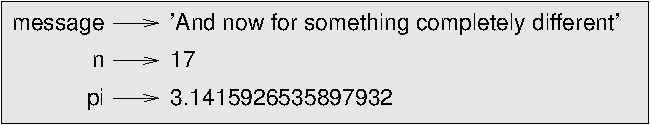
\includegraphics[scale=0.8]{../source/figs/state2.pdf}}
%🍁% \caption{State diagram.  |  状态图。}
\caption{状态图。}
\label{fig.state2}
\end{figure}

% \section{Variable names  |  变量名}
\section{变量名}
\index{variable}
\index{变量}

%🍁% Programmers generally choose names for their variables that
%🍁% are meaningful---they document what the variable is used for.
%🍁%
%🍁% Variable names can be as long as you like.  They can contain
%🍁% both letters and numbers, but they can't begin with a number.
%🍁% It is legal to use uppercase letters, but it is conventional
%🍁% to use only lower case for variables names.
%🍁%
%🍁% The underscore character, \verb"_", can appear in a name.
%🍁% It is often used in names with multiple words, such as
%🍁% \verb"your_name" or \verb"airspeed_of_unladen_swallow".
%🍁% \index{underscore character}
%🍁%
%🍁% If you give a variable an illegal name, you get a syntax error:

程序员通常为变量选择有意义的名字 --- 用于记录变量的用途。

变量名长度可以任意, 它们可以包括字母和数字,但是不能以数字开头。 使用大写字母是合法的, 但是根据惯例, 变量名只使用小写字母。

下划线 (\li{_}) 可以出现在变量名中。 它经常用于有多个单词的变量名,例如 \li{my_name} 或者 \li{airspeed_of_unladen_swallow}。
\index{underscore character} \index{下划线}

如果你给了变量一个非法的名称,解释器将抛出一个语法错误:

\begin{lstlisting}
>>> 76trombones = 'big parade'
SyntaxError: invalid syntax
>>> more@ = 1000000
SyntaxError: invalid syntax
>>> class = 'Advanced Theoretical Zymurgy'
SyntaxError: invalid syntax
\end{lstlisting}

%
%🍁% {\tt 76trombones} is illegal because it begins with a number.
%🍁% {\tt more@} is illegal because it contains an illegal character, {\tt
%🍁% @}.  But what's wrong with {\tt class}?
%🍁%
%🍁% It turns out that {\tt class} is one of Python's {\bf keywords}.  The
%🍁% interpreter uses keywords to recognize the structure of the program,
%🍁% and they cannot be used as variable names.
%🍁% \index{keyword}
%🍁%
%🍁% Python 3 has these keywords:

\li{76trombones} 是非法的,因为它以数字开头。 \li{more@} 因为包含了一个非法字符\li{@}也是非法的。 但是,\li{class} 错在哪儿了呢?

原来,\li{class} 是 Python 的 {\em 关键字} (keywords)之一。 解释器使用关键字识别程序的结构,它们不能被用作变量名。

Python 3有以下关键词:


\begin{lstlisting}
False      class      finally    is         return
None       continue   for        lambda     try
True       def        from       nonlocal   while
and        del        global     not        with
as         elif       if         or         yield
assert     else       import     pass
break      except     in         raise
\end{lstlisting}

%
%🍁% You don't have to memorize this list.  In most development environments,
%🍁% keywords are displayed in a different color; if you try to use one
%🍁% as a variable name, you'll know.

你没有必要熟记这些关键词。 大部分的开发环境会区分颜色显示关键词;如果你不小心使用关键词作为变量名,你会发现的。


% \section{Expressions and statements  |  表达式和语句}
\section{表达式和语句}

%🍁% An {\bf expression} is a combination of values, variables, and operators.
%🍁% A value all by itself is considered an expression, and so is
%🍁% a variable, so the following are all legal expressions:

{\em 表达式} (expression) 是值、变量和运算符的组合。 值和变量自身也是表达式,因此下面的表达式都是合法的:
\index{expression}  \index{表达式}

\begin{lstlisting}
>>> 42
42
>>> n
17
>>> n + 25
42
\end{lstlisting}

%
%🍁% When you type an expression at the prompt, the interpreter
%🍁% {\bf evaluates} it, which means that it finds the value of
%🍁% the expression.
%🍁% In this example, {\tt n} has the value 17 and
%🍁% {\tt n + 25} has the value 42.
%🍁% \index{evaluate}
%🍁%
%🍁% A {\bf statement} is a unit of code that has an effect, like
%🍁% creating a variable or displaying a value.
%🍁% \index{statement}

当你在提示符后输入表达式时,解释器会 {\em 计算} (evaluate) 该表达式,这就意味着解释器会求它的值。在上面的例子中,\li{n} 的值是 \li{17,n + 25} 的值是 \li{42}。
\index{evaluate}

{\em 语句} (statement) 是一个会产生影响的代码单元,例如新建一个变量或显示某个值。
\index{statement}

\begin{lstlisting}
>>> n = 17
>>> print(n)
\end{lstlisting}

%
%🍁% The first line is an assignment statement that gives a value to
%🍁% {\tt n}.  The second line is a print statement that displays the
%🍁% value of {\tt n}.
%🍁%
%🍁% When you type a statement, the interpreter {\bf executes} it,
%🍁% which means that it does whatever the statement says.  In general,
%🍁% statements don't have values.
%🍁% \index{execute}

第一行是一个赋值语句,将某个值赋给了 \li{n}。第二行是一个打印语句,在屏幕上显示 \li{n} 的值。

当你输入一个语句后,解释器会 {\em 执行} (execute) 这个语句,即按照语句的指令完成操作。一般来说,语句是没有值的。
\index{execute}

% \section{Script mode  |  脚本模式}
\section{脚本模式}

%🍁% So far we have run Python in {\bf interactive mode}, which
%🍁% means that you interact directly with the interpreter.
%🍁% Interactive mode is a good way to get started,
%🍁% but if you are working with more than a few lines of code, it can be
%🍁% clumsy.

到目前为止,我们都是在{\em 交互模式} (interactive mode) 下运行 Python,即直接与解释器进行交互。交互模式对学习入门很有帮助,但是如果你需要编写很多行代码,使用交互模式就不太方便了。

%🍁% The alternative is to save code in a file called a {\bf script} and
%🍁% then run the interpreter in {\bf script mode} to execute the script.  By
%🍁% convention, Python scripts have names that end with {\tt .py}.
%🍁% \index{script}  \index{script mode}

另一种方法是将代码保存到一个被称为脚本 (script) 的文件里,然后以脚本模式 (script mode) 运行解释器并执行脚本。按照惯例,Python脚本文件名的后缀是 \li{.py}。
\index{script}  \index{script mode}
\index{脚本}  \index{脚本模式}

%🍁% If you know how to create and run a script on your computer, you
%🍁% are ready to go.  Otherwise I recommend using PythonAnywhere again.
%🍁% I have posted instructions for running in script mode at
%🍁% \url{http://tinyurl.com/thinkpython2e}.

如果你知道如何在本地电脑新建并运行脚本,那你可以开始编码了。否则的话,我再次建议使用\hyperref[python_anywhere]{PythonAnywhere}。我在 \href{http://tinyurl.com/thinkpython2e}{http://tinyurl.com/thinkpython2e} 上贴出了如何以脚本模式运行解释器的指南。

%🍁% Because Python provides both modes,
%🍁% you can test bits of code in interactive mode before you put them
%🍁% in a script.  But there are differences between interactive mode
%🍁% and script mode that can be confusing.
%🍁% \index{interactive mode}  \index{script mode}

由于Python支持这两种模式,在将代码写入脚本之前,你可以在交互模式下对代码片段进行测试。不过,交互模式和脚本模式之间存在一些差异,可能会让你感到疑惑。
\index{interactive mode}  \index{script mode}
\index{交互模式}  \index{脚本模式}

%🍁% For example, if you are using Python as a calculator, you might type

举个例子,如果你把Python当计算器使用,你可能会输入下面这样的代码:

\begin{lstlisting}
>>> miles = 26.2
>>> miles * 1.61
42.182
\end{lstlisting}

%🍁% The first line assigns a value to {\tt miles}, but it has no visible
%🍁% effect.  The second line is an expression, so the
%🍁% interpreter evaluates it and displays the result.  It turns out that a
%🍁% marathon is about 42 kilometers.

第一行将一个值赋给 \li{miles},但是并没有产生可见的效果。 第二行是一个表达式,因此解释器计算它并将结果显示出来。 结果告诉我们,一段马拉松大概是 \li{42} 公里。

%🍁% But if you type the same code into a script and run it, you get no
%🍁% output at all.  In script mode an expression, all by itself, has no
%🍁% visible effect.  Python actually evaluates the expression, but it doesn't
%🍁% display the value unless you tell it to:

但是如果你将相同的代码键入一个脚本并且运行它,你得不到任何输出。 在脚本模式下,表达式自身不会产生可见的效果。虽然Python实际上计算了表达式,但是如果你不告诉它要显示结果,它是不会那么做的。

\begin{lstlisting}
miles = 26.2
print(miles * 1.61)
\end{lstlisting}

%🍁% This behavior can be confusing at first.
%🍁%
%🍁% A script usually contains a sequence of statements.  If there
%🍁% is more than one statement, the results appear one at a time
%🍁% as the statements execute.
%🍁%
%🍁% For example, the script

这个行为开始可能有些令人费解。

一个脚本通常包括一系列语句。 如果有多于一条的语句,那么随着语句逐个执行,解释器会逐一显示计算结果。

例如,以下脚本

\begin{lstlisting}
print(1)
x = 2
print(x)
\end{lstlisting}

%
produces the output

产生的输出结果是

\begin{lstlisting}
1
2
\end{lstlisting}

%
%🍁% The assignment statement produces no output.

%🍁% To check your understanding, type the following statements in the
%🍁% Python interpreter and see what they do:

赋值语句不产生输出。

在Python解释器中键入以下的语句,看看他们的结果是否符合你的理解:

\begin{lstlisting}
5
x = 5
x + 1
\end{lstlisting}

%🍁% Now put the same statements in a script and run it.  What
%🍁% is the output?  Modify the script by transforming each
%🍁% expression into a print statement and then run it again.

现在将同样的语句写入一个脚本中并执行它。输出结果是什么? 修改脚本,将每个表达式变成打印语句,再次运行它。

% \section{Order of operations  |  运算顺序}
\section{运算顺序}
\index{order of operations}  \index{PEMDAS}
\index{运算顺序}

%🍁% When an expression contains more than one operator, the order of
%🍁% evaluation depends on the {\bf order of operations}.  For
%🍁% mathematical operators, Python follows mathematical convention.
%🍁% The acronym {\bf PEMDAS} is a useful way to
%🍁% remember the rules:

当一个表达式中有多于一个运算符时,计算的顺序由 {\em 运算顺序} (order of operations) 决定。 对于算数运算符,Python遵循数学里的惯例。 缩写\textbf{PEMDAS}有助于帮助大家记住这些规则:

%🍁% \begin{itemize}
%🍁%
%🍁% \item {\bf P}arentheses have the highest precedence and can be used
%🍁% to force an expression to evaluate in the order you want. Since
%🍁% expressions in parentheses are evaluated first, {\tt 2 * (3-1)} is 4,
%🍁% and {\tt (1+1)**(5-2)} is 8. You can also use parentheses to make an
%🍁% expression easier to read, as in {\tt (minute * 100) / 60}, even
%🍁% if it doesn't change the result.
%🍁%
%🍁% \item {\bf E}xponentiation has the next highest precedence, so
%🍁% {\tt 1 + 2**3} is 9, not 27, and {\tt 2 * 3**2} is 18, not 36.
%🍁%
%🍁% \item {\bf M}ultiplication and {\bf D}ivision have higher precedence
%🍁%   than {\bf A}ddition and {\bf S}ubtraction.  So {\tt 2*3-1} is 5, not
%🍁%   4, and {\tt 6+4/2} is 8, not 5.
%🍁%
%🍁% \item Operators with the same precedence are evaluated from left to
%🍁%   right (except exponentiation).  So in the expression {\tt degrees /
%🍁%     2 * pi}, the division happens first and the result is multiplied
%🍁%   by {\tt pi}.  To divide by $2 \pi$, you can use parentheses or write
%🍁%   {\tt degrees / 2 / pi}.
%🍁%
%🍁% \end{itemize}

\begin{itemize}

\item {\em 括号} ({\bf P}arentheses) 具有最高的优先级,并且可以强制表达式按你希望的顺序计算。 因为在括号中的表达式首先被计算,那么 \li{2 * (3-1)} 的结果是 \li{4},\li{(1+1)**(5-2)} 的结果是 \li{8}。 你也可以用括号提高表达式的可读性,如写成 \li{(minute * 100) / 60},即使这样并不改变运算的结果。

\item {\em 指数运算} ({\bf E}xponentiation) 具有次高的优先级,因此 \li{1 + 2**3} 的结果是 \li{9} 而非 \li{27}, \li{2 * 3**2} 的结果是 \li{18} 而非 \li{36}。

\item {\em 乘法} ({\bf M}ultiplication) 和 {\em 除法} ({\bf D}ivision) 有相同的优先级, 比 {\em 加法} ({\bf A}ddition) 和 {\em 减法} ({\bf S}ubtraction) 高,加法和减法也具有相同的优先级。 因此 \li{2*3-1} 是 \li{5} 而非 \li{4}, \li{6+4/2} 是 \li{8} 而非 \li{5}。

\item 具有相同优先级的运算符按照从左到右的顺序进行计算(除了指数运算)。 因此表达式 \li{degrees / 2 * pi} 中,除法先运算,然后结果被乘以 \li{pi}。 为了被 $2\pi$ 除,你可以使用括号,或者写成 \li{degrees / 2 / pi}。

\end{itemize}

%🍁% I don't work very hard to remember the precedence of
%🍁% operators.  If I can't tell by looking at the expression, I use
%🍁% parentheses to make it obvious.

我不会费力去记住这些运算符的优先级规则。如果看完表达式后分不出优先级,我会使用括号使计算顺序变得更明显。


%
% \section{String operations  |  字符串运算}
\section{字符串运算}
\index{string!operation}  \index{operator!string}
\index{字符串!操作}  \index{操作!字符串}

%🍁% In general, you can't perform mathematical operations on strings, even
%🍁% if the strings look like numbers, so the following are illegal:

一般来讲,你不能对字符串执行数学运算,即使字符串看起来很像数字, 因此下面这些表达式是非法的:


\begin{lstlisting}
'2'-'1'    'eggs'/'easy'    'third'*'a charm'
\end{lstlisting}

%
%🍁% But there are two exceptions, {\tt +} and {\tt *}.
%🍁%
%🍁% The {\tt +} operator performs {\bf string concatenation}, which means
%🍁% it joins the strings by linking them end-to-end.  For example:

但有两个例外,\li{+} 和 \li{*}。

加号运算符 \li{+} 可用于 字符串拼接 \footnote{string concatenation},也就是将字符串首尾相连起来。例如:
\index{concatenation}

\begin{lstlisting}
>>> first = 'throat'
>>> second = 'warbler'
>>> first + second
throatwarbler
\end{lstlisting}

%
%🍁% The {\tt *} operator also works on strings; it performs repetition.
%🍁% For example, \verb"'Spam'*3" is \verb"'SpamSpamSpam'".  If one of the
%🍁% values is a string, the other has to be an integer.
%🍁%
%🍁% This use of {\tt +} and {\tt *} makes sense by
%🍁% analogy with addition and multiplication.  Just as {\tt 4*3} is
%🍁% equivalent to {\tt 4+4+4}, we expect \verb"'Spam'*3" to be the same as
%🍁% \verb"'Spam'+'Spam'+'Spam'", and it is.  On the other hand, there is a
%🍁% significant way in which string concatenation and repetition are
%🍁% different from integer addition and multiplication.
%🍁% Can you think of a property that addition has
%🍁% that string concatenation does not?
%🍁% \index{commutativity}

乘法运算符 \li{*} 也可应用于字符串;它执行重复运算。 例如,\li{'Spam'*3} 的结果是 \li{'SpamSpamSpam'}。  如果其中一个运算数是字符串,则另外一个必须是整型数。

\li{+} 和 \li{*} 的这个用法,类比加法和乘法也讲得通。 就像 \li{4*3} 与 \li{4+4+4} 等价一样, 我们也会期望 \li{'Spam'*3} 和 \li{'Spam'+'Spam'+'Spam'} 等价,而事实确实如此。 另外,字符串拼接和重复与整数的加法和乘法也有很大的不同。 你能想出来一个加法具有而字符串拼接不具有的特性么?
\index{commutativity}

% \section{Comments  |  注释}
\section{注释}
\index{comment}  \index{注释}

%🍁% As programs get bigger and more complicated, they get more difficult
%🍁% to read.  Formal languages are dense, and it is often difficult to
%🍁% look at a piece of code and figure out what it is doing, or why.
%🍁%
%🍁% For this reason, it is a good idea to add notes to your programs to explain
%🍁% in natural language what the program is doing.  These notes are called
%🍁% {\bf comments}, and they start with the \verb"#" symbol:

随着程序变得越写越长,越来越复杂,它们的可读性也越来越差。 形式语言是稠密的,通常很难在读一段代码后,说出其做什么或者为什么这样做。

因此,在你的程序中需要用自然语言做些笔记,解释程序将做些什么。 这些笔记被称为{\em 注释} (comments),以 \li{#} 符号开始。

\begin{lstlisting}
# compute the percentage of the hour that has elapsed
# 计算逝去的时间占一小时的比例
percentage = (minute * 100) / 60
\end{lstlisting}

%
%🍁% In this case, the comment appears on a line by itself.  You can also put
%🍁% comments at the end of a line:

此例中,注释独占一行。 你也可以将注释放在行尾:

\begin{lstlisting}
percentage = (minute * 100) / 60     # percentage of an hour
\end{lstlisting}

%
%🍁% Everything from the {\tt \#} to the end of the line is ignored---it
%🍁% has no effect on the execution of the program.

从 \li{#} 开始到行尾的所有内容都会被解释器忽略 — 其内容对程序执行不会有任何影响。

%🍁% Comments are most useful when they document non-obvious features of
%🍁% the code.  It is reasonable to assume that the reader can figure out
%🍁% {\em what} the code does; it is more useful to explain {\em why}.

在注释中记录代码不明显的特征,是最有帮助的。 假设读者能够读懂代码做了{\bf 什么}是合理的; 但是解释代码\textbf{为什么}这么做则更有用。

%🍁% This comment is redundant with the code and useless:

下面这个注释只是重复了代码,没有什么用:

\begin{lstlisting}
v = 5     # assign 5 to v
\end{lstlisting}

%
%🍁% This comment contains useful information that is not in the code:

下面的注释包括了代码中没有的有用信息:

\begin{lstlisting}
v = 5     # velocity in meters/second.
\end{lstlisting}

%
%🍁% Good variable names can reduce the need for comments, but
%🍁% long names can make complex expressions hard to read, so there is
%🍁% a tradeoff.

好的变量名能够减少对注释的需求,但是长变量名使得表达式很难读, 因此这里有个平衡问题。

%
% \section{Debugging  |  调试}
\section{调试}
\index{debugging}  \index{bug}
\index{调试}  \index{故障}

%🍁% Three kinds of errors can occur in a program: syntax errors, runtime
%🍁% errors, and semantic errors.  It is useful
%🍁% to distinguish between them in order to track them down more quickly.

程序中可能会出现下面三种错误:{\em 语法错误} (syntax error)、 {\em 运行时错误} (runtime error) 和 {\em 语义错误} (semantic error)。 区别三者的差异有助于快速追踪这些错误。

%🍁% \begin{description}
%🍁%
%🍁% \item[Syntax error:] ``Syntax'' refers to the structure of a program
%🍁%   and the rules about that structure.  For example, parentheses have
%🍁%   to come in matching pairs, so {\tt (1 + 2)} is legal, but {\tt 8)}
%🍁%   is a {\bf syntax error}.  \index{syntax error} \index{error!syntax}
%🍁%   \index{error message}
%🍁% \index{syntax}
%🍁%
%🍁% If there is a syntax error
%🍁% anywhere in your program, Python displays an error message and quits,
%🍁% and you will not be able to run the program.  During the first few
%🍁% weeks of your programming career, you might spend a lot of
%🍁% time tracking down syntax errors.  As you gain experience, you will
%🍁% make fewer errors and find them faster.
%🍁%
%🍁%
%🍁% \item[Runtime error:] The second type of error is a runtime error, so
%🍁%   called because the error does not appear until after the program has
%🍁%   started running.  These errors are also called {\bf exceptions}
%🍁%   because they usually indicate that something exceptional (and bad)
%🍁%   has happened.  \index{runtime error} \index{error!runtime}
%🍁%   \index{exception} \index{safe language} \index{language!safe}
%🍁%
%🍁% Runtime errors are rare in the simple programs you will see in the
%🍁% first few chapters, so it might be a while before you encounter one.
%🍁%
%🍁%
%🍁% \item[Semantic error:] The third type of error is ``semantic'', which
%🍁%   means related to meaning.  If there is a semantic error in your
%🍁%   program, it will run without generating error messages, but it will
%🍁%   not do the right thing.  It will do something else.  Specifically,
%🍁%   it will do what you told it to do.  \index{semantic error}
%🍁%   \index{error!semantic} \index{error message}
%🍁%
%🍁% Identifying semantic errors can be tricky because it requires you to work
%🍁% backward by looking at the output of the program and trying to figure
%🍁% out what it is doing.
%🍁%
%🍁% \end{description}

\begin{description}

\item[语法错误:] 语法指的是程序的结构及其背后的规则。 例如, 括号必须要成对出现, 所以 \li{(1 + 2)} 是合法的, 但是 \li{8)} 则是一个 语法错误。
\index{syntax}  \index{语法}

如果你的程序中存在一个语法错误,Python会显示一条错误信息,然后退出运行。你无法顺利运行程序。在你编程生涯的头几周里,你可能会花大量时间追踪语法错误。随着你的经验不断积累,犯的语法错误会越来越少,发现错误的速度也会更快。


\item[运行时错误:] 第二种错误类型是运行时错误,这么称呼是因为这类错误只有在程序开始运行后才会出现。这类错误也被称为 {\em 异常} (exception) ,因为它们的出现通常说明发生了某些特别的(而且不好的)事情。
  \index{runtime error} \index{error!runtime}
  \index{exception} \index{safe language} \index{language!safe}
  \index{运行时错误} \index{错误!运行时}
  \index{异常} \index{safe language} \index{language!safe}

在前几章提供的简单程序中,你很少会碰到运行时错误,所以你可能需要一段时间才会接触到这种错误。


\item[语义错误:] 第三类错误是“语义”错误,即与程序的意思的有关。如果你的程序中有语义错误,程序在运行时不会产生错误信息,但是不会返回正确的结果。它会返回另外的结果。严格来说,它是按照你的指令在运行。
  \index{semantic error}  \index{error!semantic}  \index{error message}
  \index{语义错误}  \index{错误!语义}  \index{错误信息}
识别语义错误可能是棘手的,因为这需要你反过来思考,通过观察程序的输出来搞清楚它在做什么。

\end{description}


% \section{Glossary  |  术语表}
\section{术语表}

%🍁% \begin{description}
%🍁%
%🍁% \item[variable:]  A name that refers to a value.
%🍁% \index{variable}
%🍁%
%🍁% \item[assignment:]  A statement that assigns a value to a variable.
%🍁% \index{assignment}
%🍁%
%🍁% \item[state diagram:]  A graphical representation of a set of variables and the
%🍁% values they refer to.
%🍁% \index{state diagram}
%🍁%
%🍁% \item[keyword:]  A reserved word that is used to parse a
%🍁% program; you cannot use keywords like {\tt if}, {\tt  def}, and {\tt while} as
%🍁% variable names.
%🍁% \index{keyword}
%🍁%
%🍁% \item[operand:]  One of the values on which an operator operates.
%🍁% \index{operand}
%🍁%
%🍁% \item[expression:]  A combination of variables, operators, and values that
%🍁% represents a single result.
%🍁% \index{expression}
%🍁%
%🍁% \item[evaluate:]  To simplify an expression by performing the operations
%🍁% in order to yield a single value.
%🍁%
%🍁% \item[statement:]  A section of code that represents a command or action.  So
%🍁% far, the statements we have seen are assignments and print statements.
%🍁% \index{statement}
%🍁%
%🍁% \item[execute:]  To run a statement and do what it says.
%🍁% \index{execute}
%🍁%
%🍁% \item[interactive mode:] A way of using the Python interpreter by
%🍁% typing code at the prompt.
%🍁% \index{interactive mode}
%🍁%
%🍁% \item[script mode:] A way of using the Python interpreter to read
%🍁% code from a script and run it.
%🍁% \index{script mode}
%🍁%
%🍁% \item[script:] A program stored in a file.
%🍁% \index{script}
%🍁%
%🍁% \item[order of operations:]  Rules governing the order in which
%🍁% expressions involving multiple operators and operands are evaluated.
%🍁% \index{order of operations}
%🍁%
%🍁% \item[concatenate:]  To join two operands end-to-end.
%🍁% \index{concatenation}
%🍁%
%🍁% \item[comment:]  Information in a program that is meant for other
%🍁% programmers (or anyone reading the source code) and has no effect on the
%🍁% execution of the program.
%🍁% \index{comment}
%🍁%
%🍁% \item[syntax error:]  An error in a program that makes it impossible
%🍁% to parse (and therefore impossible to interpret).
%🍁% \index{syntax error}
%🍁%
%🍁% \item[exception:]  An error that is detected while the program is running.
%🍁% \index{exception}
%🍁%
%🍁% \item[semantics:]  The meaning of a program.
%🍁% \index{semantics}
%🍁%
%🍁% \item[semantic error:]   An error in a program that makes it do something
%🍁% other than what the programmer intended.
%🍁% \index{semantic error}
%🍁%
%🍁% \end{description}

\begin{description}

\item[变量 (variable):]  变量是指向某个值的名称。
\index{variable}  \index{变量}

\item[赋值语句 (assignment):]  将某个值赋给变量的语句。
\index{assignment}  \index{赋值语句}

\item[状态图 (state diagram):]  变量及其所指的值的图形化表示。
\index{state diagram}  \index{状态图}

\item[关键字 (keyword):]  关键字是用于解析程序的;你不能使用if、def和while这样的关键词作为变量名。
\index{keyword}  \index{关键字}

\item[运算数 (operand):]  运算符所操作的值之一。
\index{operand}  \index{运算数}

\item[表达式 (expression):]  变量、运算符和值的组合,代表一个单一的结果。
\index{expression}  \index{表达式}

\item[计算 (evaluate):]  通过执行运算以简化表达式,从而得出一个单一的值。

\item[语句 (statement):]  代表一个命令或行为的一段代码。 目前为止我们接触的语句有赋值语句和打印语句。
\index{statement}  \index{语句}

\item[执行 (execute):]  运行一个语句,并按照语句的指令操作。
\index{execute}  \index{执行}

\item[交互式模式 (interactive mode):]  通过在提示符中输入代码,使用Python解释器的一种方式。
\index{interactive mode}  \index{交互式模式}

\item[脚本模式 (script mode):]  使用Python解释器从脚本中读取代码,并运行脚本的方式。
\index{script mode}  \index{脚本模式}

\item[脚本 (script):]  保存在文件中的程序。
\index{script}  \index{脚本}

\item[运算顺序 (order of operations):]  有关多个运算符和运算数时计算顺序的规则。
\index{order of operations}  \index{运算顺序}

\item[拼接 (concatenate):]  将两个运算数首尾相连。
\index{concatenation}  \index{拼接}

\item[注释 (comment):]  程序中提供给其他程序员(任何阅读源代码的人)阅读的信息,对程序的执行没有影响。
\index{comment}  \index{注释}

\item[语法错误 (syntax error):]  使得程序无法进行解析(因此无法进行解释)的错误。
\index{syntax error}  \index{语法错误}

\item[异常 (exception):]  只有在程序运行时才发现的错误。
\index{exception}  \index{异常}

\item[语义 (semantics):]  程序中表达的意思。
\index{semantics}  \index{语义}

\item[语义错误 (semantic error):]  使得程序偏离程序员原本期望的错误。
\index{semantic error}  \index{语义错误}

\end{description}


% \section{Exercises  |  练习}
\section{练习}

\begin{exercise}

%🍁% Repeating my advice from the previous chapter, whenever you learn
%🍁% a new feature, you should try it out in interactive mode and make
%🍁% errors on purpose to see what goes wrong.

%🍁% \begin{itemize}

%🍁% \item We've seen that {\tt n = 42} is legal.  What about {\tt 42 = n}?

%🍁% \item How about {\tt x = y = 1}?

%🍁% \item In some languages every statement ends with a semi-colon, {\tt ;}.
%🍁% What happens if you put a semi-colon at the end of a Python statement?

%🍁% \item What if you put a period at the end of a statement?

%🍁% \item In math notation you can multiply $x$ and $y$ like this: $x y$.
%🍁% What happens if you try that in Python?

%🍁% \end{itemize}

和上一章一样,我还是要建议大家在学习新特性之后,在交互模式下充分试验,故意犯一些错误,看看到底会出什么问题。

\begin{itemize}

\item 我们已经知道 {\em \li{n = 42}} 是合法的。那么 {\em \li{42 = n}} 呢?

\item {\em \li{x = y = 1}} 合法吗?

\item 在某些编程语言中,每个语句都是以分号 {\em \li{;}} 结束的。如果你在一个{\em Python}语句后也以分号结尾,会发生什么?

\item 如果在语句最后带上分号呢?

\item 在数学记法中,你可以将  $x$ 和  $y$ 像这样相乘: $x y$ 。如果你在 {\em Python} 中也这么写的话,会发生什么?

\end{itemize}

\end{exercise}


%
%%
\begin{exercise}

%🍁% Practice using the Python interpreter as a calculator:
%🍁% \index{calculator}

%🍁% \begin{enumerate}
%🍁%
%🍁% \item The volume of a sphere with radius $r$ is $\frac{4}{3} \pi r^3$.
%🍁%   What is the volume of a sphere with radius 5?
%🍁%
%🍁% \item Suppose the cover price of a book is \$24.95, but bookstores get a
%🍁%   40\% discount.  Shipping costs \$3 for the first copy and 75 cents
%🍁%   for each additional copy.  What is the total wholesale cost for
%🍁%   60 copies?
%🍁%
%🍁% \item If I leave my house at 6:52 am and run 1 mile at an easy pace
%🍁%   (8:15 per mile), then 3 miles at tempo (7:12 per mile) and 1 mile at
%🍁%   easy pace again, what time do I get home for breakfast?
%🍁% \index{running pace}
%🍁%
%🍁% \end{enumerate}

继续练习将 {\em Python} 解释器当做计算器使用:
\index{计算器}

\begin{enumerate}

\item 半径为 $r$ 的球体积是 $\frac{4}{3} \pi r^3$ 。 半径为 $5$ 的球体积是多少?

\item 假设一本书的零售价是 {\em \$24.95},但书店有 {\em 40\%} 的折扣。运费则是第一本 {\em \$3} ,以后每本 {\em 75} 美分。 购买 {\em 60} 本的总价是多少?

\item 如果我上午 {\em 6:52} 离开家, 以轻松跑 {\em (easy pace)}的速度跑 {\em 1} 里(即每英里耗时{\em 8}分{\em 15}秒), 再以节奏跑 {\em (tempo)} 的速度跑 {\em 3} 英里(每英里耗时{\em 7}分{\em 12}秒), 之后又以放松跑的速度跑 {\em 1} 英里, 我什么时候回到家吃早饭? \footnote{译者注:配速(pace)是在马拉松运动的训练中常使用的一个概念,配速是速度的一种,是每公里所需要的时间。配速=时间/距离。Tempo run 一般被翻译成「节奏跑」或「乳酸门槛跑」,是指以比10K或5K比赛速度稍慢(每公里大约慢10--15秒)的速度进行训练,或者以平时15K-半程的配速来跑。参考:https://www.zhihu.com/question/22237002}
\index{running pace}

\end{enumerate}

\end{exercise}



% \chapter{Functions  |  函数}
\chapter{函数}
\label{funcchap}

%🍁% In the context of programming, a {\bf function} is a named sequence of
%🍁% statements that performs a computation.  When you define a function,
%🍁% you specify the name and the sequence of statements.  Later, you can
%🍁% ``call'' the function by name.
%🍁% \index{function}

在编程的语境下,{\em 函数} (function)  是指一个有命名的、执行某个计算的语句序列(sequence of statements) 。  在定义一个函数的时候,你需要指定函数的名字和语句序列。  之后,你可以通过这个名字``{\em 调用} (call)''该函数。
\index{function}  \index{函数}

%
%%
% \section{Function calls  |  函数调用}
\section{函数调用}
\label{functionchap}
\index{function call}
\index{函数调用}

%🍁% We have already seen one example of a {\bf function call}:

我们已经看见过了 {\em 函数调用} (function call) 的例子。

\begin{lstlisting}
>>> type(42)
<class 'int'>
\end{lstlisting}

%
%🍁% The name of the function is {\tt type}.  The expression in parentheses
%🍁% is called the {\bf argument} of the function.  The result, for this
%🍁% function, is the type of the argument.

这个函数的名字是 ``type''。 括号中的表达式被称为这个函数的 {\em 实参} (argument)。 这个函数执行的结果,就是实参的类型。
\index{parentheses!argument in}
\index{括号!实参}

%🍁% It is common to say that a function ``takes'' an argument and ``returns''
%🍁% a result.  The result is also called the {\bf return value}.

人们常说函数``接受 (accept)''实参,然后 ``返回 (return)''一个结果。
该结果也被称为 {\em 返回值} (return value)。
\index{argument}  \index{return value}
\index{实参}  \index{返回值}

%🍁% Python provides functions that convert values
%🍁% from one type to another.  The {\tt int} function takes any value and
%🍁% converts it to an integer, if it can, or complains otherwise:

Python提供了能够将值从一种类型转换为另一种类型的内建函数。
函数 \li{int} 接受任意值,并在其能做到的情况下,将该值转换成一个整型数,
否则会报错:
\index{conversion!type}  \index{type conversion}
\index{int function}  \index{function!int}
\index{转换!类型}  \index{类型转换}
\index{整数型函数}  \index{函数!整数型}

\begin{lstlisting}
>>> int('32')
32
>>> int('Hello')
ValueError: invalid literal for int(): Hello
\end{lstlisting}

%
%🍁% {\tt int} can convert floating-point values to integers, but it
%🍁% doesn't round off; it chops off the fraction part:

\li{int} 能将浮点数转换为整型数,但是它并不进行舍入;只是截掉了小数点部分:

\begin{lstlisting}
>>> int(3.99999)
3
>>> int(-2.3)
-2
\end{lstlisting}

%
%🍁% {\tt float} converts integers and strings to floating-point
%🍁% numbers:

\li{float} 可以将整型数和字符串转换为浮点数:
\index{float function}  \index{function!float}
\index{浮点型函数}  \index{函数!浮点型}

\begin{lstlisting}
>>> float(32)
32.0
>>> float('3.14159')
3.14159
\end{lstlisting}

%
%🍁% Finally, {\tt str} converts its argument to a string:

\li{str} 可以将其实参转换成字符串:
\index{str function}  \index{function!str}
\index{字符串函数}  \index{函数!字符串}

\begin{lstlisting}
>>> str(32)
'32'
>>> str(3.14159)
'3.14159'
\end{lstlisting}

%
%%
% \section{Math functions  |  数学函数}
\section{数学函数}
\index{math function}  \index{function, math}
\index{数学函数}  \index{函数, 数学}


%🍁% Python has a math module that provides most of the familiar
%🍁% mathematical functions.  A {\bf module} is a file that contains a
%🍁% collection of related functions.

Python中有一个数学函数模块,提供了大部分常用的数学函数。
{\em 模块} (module) 是指一个包含相关函数集合的文件。
\index{module}  \index{module object}
\index{模块}  \index{模块对象}

%🍁% Before we can use the functions in a module, we have to import it with
%🍁% an {\bf import statement}:

在使用模块之前,我们需要通过 {\em 导入语句} (import statement) 导入该模块:

\begin{lstlisting}
>>> import math
\end{lstlisting}

%
%🍁% This statement creates a {\bf module object} named math.  If
%🍁% you display the module object, you get some information about it:

这条语句会生成一个名为 ``math'' 的 {\em 模块对象} (module object) 。
如果你打印这个模块对象,你将获得关于它的一些信息:


\begin{lstlisting}
>>> math
<module 'math' (built-in)>
\end{lstlisting}

%
%🍁% The module object contains the functions and variables defined in the
%🍁% module.  To access one of the functions, you have to specify the name
%🍁% of the module and the name of the function, separated by a dot (also
%🍁% known as a period).  This format is called {\bf dot notation}.

该模块对象包括了定义在模块内的所有函数和变量。
想要访问其中的一个函数,你必须指定该模块的名字以及函数名,
并以点号(也被叫做句号)分隔开来。 这种形式被称作 {\em 点标记法} (dot
notation)。
\index{dot notation}  \index{点标记法}

\begin{lstlisting}
>>> ratio = signal_power / noise_power
>>> decibels = 10 * math.log10(ratio)

>>> radians = 0.7
>>> height = math.sin(radians)
\end{lstlisting}

%
%🍁% The first example uses \verb"math.log10" to compute
%🍁% a signal-to-noise ratio in decibels (assuming that \verb"signal_power" and
%🍁% \verb"noise_power" are defined).  The math module also provides {\tt log},
%🍁% which computes logarithms base {\tt e}.

第一个例子使用\li{math.log10} 计算分贝信噪比(假设 \li{signal_power}  和\li{noise_power} 已经被定义了)。
math 模块也提供了 \li{log} 函数,用于计算以 $e$ 为底的对数。
\index{log function}  \index{function!log}  \index{sine function}
\index{radian}  \index{trigonometric function}  \index{function, trigonometric}

%🍁% The second example finds the sine of {\tt radians}.  The name of the
%🍁% variable is a hint that {\tt sin} and the other trigonometric
%🍁% functions ({\tt cos}, {\tt tan}, etc.)  take arguments in radians. To
%🍁% convert from degrees to radians, divide by 180 and multiply by
%🍁% $\pi$:

第二个例子计算 \li{radians} 的正弦值。
变量名暗示了 \li{sin} 及其它三角函数( \li{cos}、\li{tan} 等)接受弧度(radians)实参。 度数转换为弧度,需要除以$180$,并乘以 $\pi$ :


\begin{lstlisting}
>>> degrees = 45
>>> radians = degrees / 180.0 * math.pi
>>> math.sin(radians)
0.707106781187
\end{lstlisting}

%
%🍁% The expression {\tt math.pi} gets the variable {\tt pi} from the math
%🍁% module.  Its value is a floating-point approximation
%🍁% of $\pi$, accurate to about 15 digits.

表达式 \li{math.pi} 从 \li{math} 模块中获得变量 \li{pi} 。
该变量的值是 $\pi$ 的一个浮点数近似值,精确到大约15位数。
\index{pi}  \index{$\pi$}
\index{圆周率}

%🍁% If you know trigonometry, you can check the previous result by comparing it to the square root of two divided by two:

如果你了解懂几何学 (trigonometry) ,你可以将之前的结果和二分之根号二进行比较,检查是否正确:
\index{sqrt function}  \index{function!sqrt}

\begin{lstlisting}
>>> math.sqrt(2) / 2.0
0.707106781187
\end{lstlisting}
%

%
%%
% \section{Composition  |  构建}
\section{构建}
\index{composition}

%🍁% So far, we have looked at the elements of a program---variables,
%🍁% expressions, and statements---in isolation, without talking about how to
%🍁% combine them.

目前为止,我们已经分别介绍了程序的基本元素 --- 变量、表达式和语句,但是还没有讨论如何将它们组合在一起。

%🍁% One of the most useful features of programming languages is their
%🍁% ability to take small building blocks and {\bf compose} them.  For
%🍁% example, the argument of a function can be any kind of expression,
%🍁% including arithmetic operators:

编程语言的最有用特征之一,是能够将小块构建材料 (building blocks) {\em 构建} (compose) 在一起。
例如,函数的实参可以是任意类型的表达式,包括算术运算符:

\begin{lstlisting}
x = math.sin(degrees / 360.0 * 2 * math.pi)
\end{lstlisting}

%
%🍁% And even function calls:

甚至是函数调用:

\begin{lstlisting}
x = math.exp(math.log(x+1))
\end{lstlisting}

%
%🍁% Almost anywhere you can put a value, you can put an arbitrary
%🍁% expression, with one exception: the left side of an assignment
%🍁% statement has to be a variable name.  Any other expression on the left
%🍁% side is a syntax error (we will see exceptions to this rule
%🍁% later).

几乎任何可以放一个值的地方,都可以放一个任意类型的表达式,除了一个例外:
赋值语句的左侧必须是一个变量名。左侧放其他任何表达式都会产生语法错误
(后面我们会讲到这个规则的例外)。

\begin{lstlisting}
>>> minutes = hours * 60                 # right
>>> hours * 60 = minutes                 # wrong!
SyntaxError: can't assign to operator
\end{lstlisting}
%
\index{SyntaxError}  \index{exception!SyntaxError}
\index{语法错误}  \index{异常!语法错误}

%
%%
% \section{Adding new functions  |  增加新函数}
\section{增加新函数}

%🍁% So far, we have only been using the functions that come with Python,
%🍁% but it is also possible to add new functions.
%🍁% A {\bf function definition} specifies the name of a new function and
%🍁% the sequence of statements that run when the function is called.

目前为止,我们只使用了 Python 自带的函数, 但是增加新函数也是可能的。
一个 {\em 函数定义} (function definition) 指定了新函数的名称
以及当函数被调用时执行的语句序列。
\index{function}  \index{function definition}  \index{definition!function}
\index{函数}  \index{函数定义}  \index{定义!函数}

%🍁% Here is an example:

下面是一个示例:


\begin{lstlisting}
def print_lyrics():
    print("I'm a lumberjack, and I'm okay.")
    print("I sleep all night and I work all day.")
\end{lstlisting}

%
%🍁% {\tt def} is a keyword that indicates that this is a function
%🍁% definition.  The name of the function is \verb"print_lyrics".  The
%🍁% rules for function names are the same as for variable names: letters,
%🍁% numbers and underscore are legal, but the first character
%🍁% can't be a number.  You can't use a keyword as the name of a function,
%🍁% and you should avoid having a variable and a function with the same
%🍁% name.

\li{def} 是一个关键字,表明这是一个函数定义。
这个函数的名字是 \li{print_lyrics}。
函数的命名规则与变量名相同:字母、数字以及下划线是合法的,
但是第一个字符不能是数字。不能使用关键字作为函数名,并应该避免
变量和函数同名。
\index{def keyword}  \index{keyword!def}  \index{argument}

The empty parentheses after the name indicate that this function
doesn't take any arguments.

函数名后面的圆括号是空的,表明该函数不接受任何实参。
\index{parentheses!empty}  \index{header}
\index{body}  \index{indentation}  \index{colon}

%🍁% The first line of the function definition is called the {\bf header};
%🍁% the rest is called the {\bf body}.  The header has to end with a colon
%🍁% and the body has to be indented.  By convention, indentation is
%🍁% always four spaces.  The body can contain
%🍁% any number of statements.

函数定义的第一行被称作 {\em 函数头} (header); 其余部分被称作 {\em 函数体} (body)。 函数头必须以冒号结尾,而函数体必须缩进。 按照惯例,缩进总是4个空格。 函数体能包含任意条语句。

%🍁% The strings in the print statements are enclosed in double
%🍁% quotes.  Single quotes and double quotes do the same thing;
%🍁% most people use single quotes except in cases like this where
%🍁% a single quote (which is also an apostrophe) appears in the string.

打印语句中的字符串被括在双引号中。单引号和双引号的作用相同;大多数人使用单引号,上述代码中的情况除外,即单引号(同时也是撇号)出现在字符串中时。

%🍁% All quotation marks (single and double)
%🍁% must be ``straight quotes'', usually
%🍁% located next to Enter on the keyboard.  ``Curly quotes'', like
%🍁% the ones in this sentence, are not legal in Python.

所有引号(单引号和双引号)必须是"{\em 直引号}" (straight quotes),它们通常位于键盘上 Enter 键的旁边。像这句话中使用的 ``{\em 弯引号}'' (curly quotes), 在 Python 语言中则是不合法的。

%🍁% If you type a function definition in interactive mode, the interpreter
%🍁% prints dots ({\tt ...}) to let you know that the definition
%🍁% isn't complete:

如果你在交互模式下键入函数定义,每空一行解释器就会打印三个句点 \li{...},
让你知道定义并没有结束。
\index{ellipses}

\begin{lstlisting}
>>> def print_lyrics():
...     print("I'm a lumberjack, and I'm okay.")
...     print("I sleep all night and I work all day.")
...
\end{lstlisting}

%
%🍁% To end the function, you have to enter an empty line.

为了结束函数定义,你必须输入一个空行。

%🍁% Defining a function creates a {\bf function object}, which
%🍁% has type \verb"function":

定义一个函数会创建一个 {\em 函数对象} (function object),其类型是 \li{function}:
\index{function type}  \index{type!function}
\index{函数类型}  \index{类型!函数}

\begin{lstlisting}
>>> print(print_lyrics)
<function print_lyrics at 0xb7e99e9c>
>>> type(print_lyrics)
<class 'function'>
\end{lstlisting}

%
%🍁% The syntax for calling the new function is the same as
%🍁% for built-in functions:

调用新函数的语法,和调用内建函数的语法相同:

\begin{lstlisting}
>>> print_lyrics()
I'm a lumberjack, and I'm okay.
I sleep all night and I work all day.
\end{lstlisting}

%
%🍁% Once you have defined a function, you can use it inside another
%🍁% function.  For example, to repeat the previous refrain, we could write
%🍁% a function called \verb"repeat_lyrics":

一旦你定义了一个函数,你就可以在另一个函数内部使用它。
例如,为了重复之前的叠句 (refrain),我们可以编写一个名叫 \li{repeat_lyrics} :


\begin{lstlisting}
def repeat_lyrics():
    print_lyrics()
    print_lyrics()
\end{lstlisting}

%
%🍁% And then call \verb"repeat_lyrics":

然后调用 \li{repeat_lyrics}


\begin{lstlisting}
>>> repeat_lyrics()
I'm a lumberjack, and I'm okay.
I sleep all night and I work all day.
I'm a lumberjack, and I'm okay.
I sleep all night and I work all day.
\end{lstlisting}

%
%🍁% But that's not really how the song goes.

不过,这首歌的歌词实际上不是这样的。


%
%%
% \section{Definitions and uses  |  定义和使用}
\section{定义和使用}
\index{function definition}
\index{函数定义}

%🍁% Pulling together the code fragments from the previous section, the
%🍁% whole program looks like this:

将上一节的多个代码段组合在一起,整个程序看起来是这样的:

\begin{lstlisting}
def print_lyrics():
    print("I'm a lumberjack, and I'm okay.")
    print("I sleep all night and I work all day.")

def repeat_lyrics():
    print_lyrics()
    print_lyrics()

repeat_lyrics()
\end{lstlisting}

%
%🍁% This program contains two function definitions: \verb"print_lyrics" and
%🍁% \verb"repeat_lyrics".  Function definitions get executed just like other
%🍁% statements, but the effect is to create function objects.  The statements
%🍁% inside the function do not run until the function is called, and
%🍁% the function definition generates no output.

该程序包含两个函数定义:\li{print_lyrics} 和 \li{repeat_lyrics}。
函数定义和其它语句一样,都会被执行,但是其作用是创建函数对象。
函数内部的语句在函数被调用之前,是不会执行的,而且函数定义不会产生任何输出。
\index{use before def}

%🍁% As you might expect, you have to create a function before you can
%🍁% run it.  In other words, the function definition has to run
%🍁% before the function gets called.

你可能猜到了,在运行函数之前,你必须先创建这个函数。换句话说,函数定义必须在其第一次被调用之前执行。

%🍁% As an exercise, move the last line of this program
%🍁% to the top, so the function call appears before the definitions. Run
%🍁% the program and see what error
%🍁% message you get.

我们做个小练习,将程序的最后一行移到顶部,使得函数调用出现在函数定义之前。运行程序,看看会得到怎样的错误信息。


%🍁% Now move the function call back to the bottom
%🍁% and move the definition of \verb"print_lyrics" after the definition of
%🍁% \verb"repeat_lyrics".  What happens when you run this program?

现在将函数调用移回底部,然后将 \li{print_lyrics} 的定义移到 \li{repeat_lyrics} 的定义之后。这次运行程序时会发生什么?


%
%%
% \section{Flow of execution  |  执行流程}
\section{执行流程}
\index{flow of execution}  \index{执行流程}

%🍁% To ensure that a function is defined before its first use,
%🍁% you have to know the order statements run in, which is
%🍁% called the {\bf flow of execution}.

为了保证函数第一次使用之前已经被定义,你必须要了解语句执行的顺序,
这也被称作 {\em 执行流程} (flow of execution) 。

%🍁% Execution always begins at the first statement of the program.
%🍁% Statements are run one at a time, in order from top to bottom.

执行流程总是从程序的第一条语句开始,自顶向下,每次执行一条语句。

%🍁% Function definitions do not alter the flow of execution of the
%🍁% program, but remember that statements inside the function don't
%🍁% run until the function is called.

函数定义不改变程序执行的流程,但是请记住,函数不被调用的话,函数内部的语句是不会执行的。

%🍁% A function call is like a detour in the flow of execution. Instead of
%🍁% going to the next statement, the flow jumps to the body of
%🍁% the function, runs the statements there, and then comes back
%🍁% to pick up where it left off.

函数调用像是在执行流程上绕了一个弯路。
执行流程没有进入下一条语句,而是跳入了函数体,开始执行那里的语句,然后再回到它离开的位置。

%🍁% That sounds simple enough, until you remember that one function can
%🍁% call another.  While in the middle of one function, the program might
%🍁% have to run the statements in another function.  Then, while
%🍁% running that new function, the program might have to run yet
%🍁% another function!

这听起来足够简单,至少在你想起一个函数可以调用另一个函数之前。
当一个函数执行到中间的时候,程序可能必须执行另一个函数里的语句。
然后在执行那个新函数的时候,程序可能又得执行另外一个函数!

%🍁% Fortunately, Python is good at keeping track of where it is, so each
%🍁% time a function completes, the program picks up where it left off in
%🍁% the function that called it.  When it gets to the end of the program,
%🍁% it terminates.

幸运的是,Python善于记录程序执行流程的位置,因此每次一个函数执行完成时,
程序会回到调用它的那个函数原来执行的位置。当到达程序的结尾时,程序才会终止。

%🍁% In summary, when you read a program, you
%🍁% don't always want to read from top to bottom.  Sometimes it makes
%🍁% more sense if you follow the flow of execution.

总之,阅读程序时,你没有必要总是从上往下读。有时候,跟着执行流程阅读反而更加合理。


%
%%
% \section{Parameters and arguments  |  形参和实参}
\section{形参和实参}
\label{parameters}
\index{parameter}  \index{function parameter}
\index{argument}  \index{function argument}

%🍁% Some of the functions we have seen require arguments.  For
%🍁% example, when you call {\tt math.sin} you pass a number
%🍁% as an argument.  Some functions take more than one argument:
%🍁% {\tt math.pow} takes two, the base and the exponent.

我们之前接触的一些函数需要实参。例如,当你调用 \li{math.sin} 时,你传递一个数字作为实参。
有些函数接受一个以上的实参: \li{math.pow} 接受两个,底数和指数。

%🍁% Inside the function, the arguments are assigned to
%🍁% variables called {\bf parameters}.  Here is a definition for
%🍁% a function that takes an argument:
%🍁% \index{parentheses!parameters in}

在函数内部,实参被赋给称作 {\em 形参} (parameters) 的变量。
下面的代码定义了一个接受一个实参的函数:
\index{parentheses!parameters in}

\begin{lstlisting}
def print_twice(bruce):
    print(bruce)
    print(bruce)
\end{lstlisting}

%
%🍁% This function assigns the argument to a parameter
%🍁% named {\tt bruce}.  When the function is called, it prints the value of
%🍁% the parameter (whatever it is) twice.

这个函数将实参赋给名为 \li{bruce} 的形参。当函数被调用的时候,它会打印形参(无论它是什么)的值两次。

%🍁% This function works with any value that can be printed.

该函数对任意能被打印的值都有效。

\begin{lstlisting}
>>> print_twice('Spam')
Spam
Spam
>>> print_twice(42)
42
42
>>> print_twice(math.pi)
3.14159265359
3.14159265359
\end{lstlisting}

%
%🍁% The same rules of composition that apply to built-in functions also
%🍁% apply to programmer-defined functions, so we can use any kind of expression
%🍁% as an argument for \verb"print_twice":

组合规则不仅适用于内建函数,而且也适用于开发者自定义的函数(programmer-defined functions),因此我们可以使用任意类型的表达式作为 \li{print_twice} 的实参:
\index{composition}  \index{programmer-defined function}
\index{function!programmer defined}

\begin{lstlisting}
>>> print_twice('Spam '*4)
Spam Spam Spam Spam
Spam Spam Spam Spam
>>> print_twice(math.cos(math.pi))
-1.0
-1.0
\end{lstlisting}

%
%🍁% The argument is evaluated before the function is called, so
%🍁% in the examples the expressions \verb"'Spam '*4" and
%🍁% {\tt math.cos(math.pi)} are only evaluated once.

在函数被调用之前,实参会先进行计算,因此在这些例子中,
表达式 \li{Spam '*4} 和 \li{math.cos(math.pi)} 都只被计算了一次。
\index{argument}

%🍁% You can also use a variable as an argument:

你也可以用变量作为实参:

\begin{lstlisting}
>>> michael = 'Eric, the half a bee.'
>>> print_twice(michael)
Eric, the half a bee.
Eric, the half a bee.
\end{lstlisting}

%
%🍁% The name of the variable we pass as an argument ({\tt michael}) has
%🍁% nothing to do with the name of the parameter ({\tt bruce}).  It
%🍁% doesn't matter what the value was called back home (in the caller);
%🍁% here in \verb"print_twice", we call everybody {\tt bruce}.

我们传递的实参名 \li{michael} 与形参的名字 \li{bruce} 没有任何关系。 这个值在传入函数之前叫什么都没有关系;只要传入了 \li{print_twice} 函数,我们将所有人都称为 \li{bruce}。


%
%%
% \section{Variables and parameters are local  |  变量和形参都是局部的}
\section{变量和形参都是局部的}
\index{local variable}  \index{variable!local}
\index{局部变量}  \index{变量!局部变量}

%🍁% When you create a variable inside a function, it is {\bf local},
%🍁% which means that it only
%🍁% exists inside the function.  For example:

当你在函数里面创建变量时,这个变量是 {\em 局部}的 (local),
也就是说它只在函数内部存在。 例如:
\index{parentheses!parameters in}

\begin{lstlisting}
def cat_twice(part1, part2):
    cat = part1 + part2
    print_twice(cat)
\end{lstlisting}

%
%🍁% This function takes two arguments, concatenates them, and prints
%🍁% the result twice.  Here is an example that uses it:

该函数接受两个实参,拼接 (concatenates) 它们并打印结果两次。 下面是使用该函数的一个示例:
\index{concatenation}

\begin{lstlisting}
>>> line1 = 'Bing tiddle '
>>> line2 = 'tiddle bang.'
>>> cat_twice(line1, line2)
Bing tiddle tiddle bang.
Bing tiddle tiddle bang.
\end{lstlisting}

%
%🍁% When \verb"cat_twice" terminates, the variable {\tt cat}
%🍁% is destroyed.  If we try to print it, we get an exception:
%🍁% \index{NameError}  \index{exception!NameError}

当 \li{cat_twice} 结束时,变量 \li{cat} 被销毁了。
如果我们试图打印它,我们将获得一个异常:
\index{NameError}  \index{exception!NameError}

\begin{lstlisting}
>>> print(cat)
NameError: name 'cat' is not defined
\end{lstlisting}

%
%🍁% Parameters are also local.
%🍁% For example, outside \verb"print_twice", there is no
%🍁% such thing as {\tt bruce}.

形参也都是局部的。例如,在 \li{print_twice} 函数的外部并没有 \li{bruce} 这个变量。
\index{parameter}
\index{形参}


%
%%
% \section{Stack diagrams  |  堆栈图}
\section{堆栈图}
\label{stackdiagram}
\index{stack diagram}  \index{function frame}  \index{frame}
\index{堆栈图}  \index{function frame}  \index{frame}

%🍁% To keep track of which variables can be used where, it is sometimes
%🍁% useful to draw a {\bf stack diagram}.  Like state diagrams, stack
%🍁% diagrams show the value of each variable, but they also show the
%🍁% function each variable belongs to.

有时, 画一个 {\em 堆栈图} (stack diagram) 可以帮助你跟踪哪个变量能在哪儿用。  
与状态图类似, 堆栈图要说明每个变量的值, 但是它们也要说明每个变量所属的函数。  
\index{stack diagram}  \index{diagram!stack}

%🍁% Each function is represented by a {\bf frame}.  A frame is a box with
%🍁% the name of a function beside it and the parameters and variables of
%🍁% the function inside it.  The stack diagram for the previous example is
%🍁% shown in Figure~\ref{fig.stack}.

每个函数用一个 {\em 栈帧} (frame) 表示。
一个栈帧就是一个线框,函数名在旁边,形参以及函数内部的变量则在里面。
前面例子的堆栈图如图~\ref{fig.stack}所示。

\begin{figure}
\centerline
{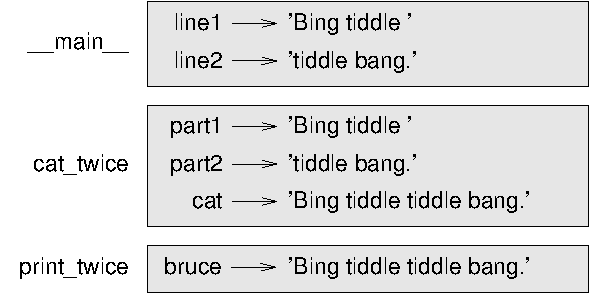
\includegraphics[scale=0.8]{../source/figs/stack.pdf}}
%🍁% \caption{Stack diagram.}
\caption{堆栈图。}
\label{fig.stack}
\end{figure}

%🍁% The frames are arranged in a stack that indicates which function
%🍁% called which, and so on.  In this example, \verb"print_twice"
%🍁% was called by \verb"cat_twice", and \verb"cat_twice" was called by
%🍁% \verb"__main__", which is a special name for the topmost frame.  When
%🍁% you create a variable outside of any function, it belongs to
%🍁% \verb"__main__".

这些线框排列成栈的形式,说明了哪个函数调用了哪个函数等信息。
在此例中,\li{print_twice} 被 \li{cat_twice} 调用,
\li{cat_twice} 又被 \li{__main__} 调用, \li{__main__} 是一个表示最上层栈帧的特殊名字。
当你在所有函数之外创建一个变量时,它就属于 \li{__main__}。

%🍁% Each parameter refers to the same value as its corresponding
%🍁% argument.  So, {\tt part1} has the same value as
%🍁% {\tt line1}, {\tt part2} has the same value as {\tt line2},
%🍁% and {\tt bruce} has the same value as {\tt cat}.

每个形参都指向其对应实参的值。
因此,\li{part1} 和 \li{line1} 的值相同, \li{part2} 和 \li{line2} 的值相同, \li{bruce} 和 \li{cat} 的值相同。

%🍁% If an error occurs during a function call, Python prints the
%🍁% name of the function, the name of the function that called
%🍁% it, and the name of the function that called {\em that}, all the
%🍁% way back to \verb"__main__".

如果函数调用时发生错误,Python会打印出错函数的名字以及调用它的函数的名字,
以及调用 *后面这个函数* 的函数的名字,一直追溯到 \li{__main__} 为止。

%🍁% For example, if you try to access {\tt cat} from within
%🍁% \verb"print_twice", you get a {\tt NameError}:

例如,如果你试图在 \li{print_twice} 里面访问 \li{cat} ,
你将获得一个 \li{NameError} :

%🍁% \begin{lstlisting}
%🍁% Traceback (innermost last):
%🍁%   File "test.py", line 13, in __main__
%🍁%     cat_twice(line1, line2)
%🍁%   File "test.py", line 5, in cat_twice
%🍁%     print_twice(cat)
%🍁%   File "test.py", line 9, in print_twice
%🍁%     print(cat)
%🍁% NameError: name 'cat' is not defined
%🍁% \end{lstlisting}
%🍁%

%🍁% This list of functions is called a {\bf traceback}.  It tells you what
%🍁% program file the error occurred in, and what line, and what functions
%🍁% were executing at the time.  It also shows the line of code that
%🍁% caused the error.

这个函数列表被称作 {\em 回溯} (traceback) 。
它告诉你发生错误的是哪个程序文件,错误在哪一行,以及当时在执行哪个函数。
它还会显示引起错误的那一行代码。
\index{traceback}

%🍁% The order of the functions in the traceback is the same as the
%🍁% order of the frames in the stack diagram.  The function that is
%🍁% currently running is at the bottom.

回溯中的函数顺序,与堆栈图中的函数顺序一致。出错时正在运行的那个函数则位于回溯信息的底部。


%
%%
% \section{Fruitful functions and void functions  |  有返回值函数和无返回值函数}
\section{有返回值函数和无返回值函数}
\index{fruitful function}  \index{void function}
\index{function, fruitful}  \index{function, void}
\index{有返回值函数}  \index{无返回值函数}
\index{函数function, 有返回值}  \index{函数, 无返回值}


%🍁% Some of the functions we have used, such as the math functions, return
%🍁% results; for lack of a better name, I call them {\bf fruitful
%🍁%   functions}.  Other functions, like \verb"print_twice", perform an
%🍁% action but don't return a value.  They are called {\bf void
%🍁%   functions}.

有一些我们之前用过的函数,例如数学函数,会返回结果;
由于没有更好的名字,我姑且叫它们 {\em 有返回值函数} (fruitful functions) 。
其它的函数,像 \li{print_twice} ,执行一个动作但是不返回任何值。
我称它们为 {\em 无返回值函数} (void functions) 。

%🍁% When you call a fruitful function, you almost always
%🍁% want to do something with the result; for example, you might
%🍁% assign it to a variable or use it as part of an expression:

当你调用一个有返回值函数时,你几乎总是想用返回的结果去做些什么;
例如,你可能将它赋值给一个变量,或者把它用在表达式里:

\begin{lstlisting}
x = math.cos(radians)
golden = (math.sqrt(5) + 1) / 2
\end{lstlisting}

%
%🍁% When you call a function in interactive mode, Python displays
%🍁% the result:

当你在交互模式下调用一个函数时,Python解释器会马上显示结果:

\begin{lstlisting}
>>> math.sqrt(5)
2.2360679774997898
\end{lstlisting}

%
%🍁% But in a script, if you call a fruitful function all by itself,
%🍁% the return value is lost forever!

但是在脚本中,如果你单单调用一个有返回值函数, 返回值就永远丢失了!

\begin{lstlisting}
math.sqrt(5)
\end{lstlisting}

%
%🍁% This script computes the square root of 5, but since it doesn't store
%🍁% or display the result, it is not very useful.

该脚本计算5的平方根,但是因为它没保存或者显示这个结果,
这个脚本并没多大用处。
\index{interactive mode}  \index{script mode}

%🍁% Void functions might display something on the screen or have some
%🍁% other effect, but they don't have a return value.  If you
%🍁% assign the result to a variable, you get a special value called
%🍁% {\tt None}.

无返回值函数可能在屏幕上打印输出结果,或者产生其它的影响,
但是它们并没有返回值。如果你试图将无返回值函数的结果赋给一个变量,
你会得到一个被称作 \li{None} 的特殊值。
\index{None special value}  \index{special value!None}

\begin{lstlisting}
>>> result = print_twice('Bing')
Bing
Bing
>>> print(result)
None
\end{lstlisting}

%
%🍁% The value {\tt None} is not the same as the string \verb"'None'".
%🍁% It is a special value that has its own type:

\li{None} 这个值和字符串 \li{'None'} 不同。 这是一个具有独立类型的特殊值:

\begin{lstlisting}
>>> print(type(None))
<class 'NoneType'>
\end{lstlisting}

%
%🍁% The functions we have written so far are all void.  We will start
%🍁% writing fruitful functions in a few chapters.

目前为止,我们写的函数都是无返回值函数。
我们将在几章之后开始编写有返回值函数。
\index{NoneType type}  \index{type!NoneType}


%
%%
% \section{Why functions?  |  为什么使用函数?}
\section{为什么使用函数?}
\index{function, reasons for}

%🍁% It may not be clear why it is worth the trouble to divide
%🍁% a program into functions.  There are several reasons:

%🍁% \begin{itemize}
%🍁%
%🍁% \item Creating a new function gives you an opportunity to name a group
%🍁% of statements, which makes your program easier to read and debug.
%🍁%
%🍁% \item Functions can make a program smaller by eliminating repetitive
%🍁% code.  Later, if you make a change, you only have
%🍁% to make it in one place.
%🍁%
%🍁% \item Dividing a long program into functions allows you to debug the
%🍁% parts one at a time and then assemble them into a working whole.
%🍁%
%🍁% \item Well-designed functions are often useful for many programs.
%🍁% Once you write and debug one, you can reuse it.
%🍁%
%🍁% \end{itemize}

你可能还不明白为什么值得将一个程序分解成多个函数。 原因包括以下几点:

\begin{itemize}

\item 创建一个新的函数可以让你给一组语句命名,这可以让你的程序更容易阅读和调试。

\item 通过消除重复的代码,函数精简了程序。 以后,如果你要做个变动,你只需在一处修改即可。

\item 将一个长程序分解为多个函数,可以让你一次调试一部分,然后再将它们组合为一个可行的整体。

\item 设计良好的函数经常对多个程序都有帮助。一旦你写出并调试好一个函数,你就可以重复使用它。

\end{itemize}


%
%%
% \section{Debugging  |  调试}
\section{调试}
\index{debug]}  \index{调试}

%🍁% One of the most important skills you will acquire is debugging.
%🍁% Although it can be frustrating, debugging is one of the most
%🍁% intellectually rich, challenging, and interesting parts of
%🍁% programming.

调试,是你能获得的最重要的技能之一。
虽然调试会让人沮丧,但却是编程过程中最富含智慧、挑战以及乐趣的一部分。
\index{experimental debugging}  \index{debugging!experimental}

%🍁% In some ways debugging is like detective work.  You are confronted
%🍁% with clues and you have to infer the processes and events that led
%🍁% to the results you see.

在某些方面,调试像是侦探工作。
你面对一些线索,必须推理出是什么进程 (processes) 和事件 (events)导致了你看到的结果。

%🍁% Debugging is also like an experimental science.  Once you have an idea
%🍁% about what is going wrong, you modify your program and try again.  If
%🍁% your hypothesis was correct, you can predict the result of the
%🍁% modification, and you take a step closer to a working program.  If
%🍁% your hypothesis was wrong, you have to come up with a new one.  As
%🍁% Sherlock Holmes pointed out, ``When you have eliminated the
%🍁% impossible, whatever remains, however improbable, must be the truth.''
%🍁% (A. Conan Doyle, {\em The Sign of Four})

调试也像是一门实验性科学。一旦你猜到大概哪里出错了,
你可以修改程序,再试一次。
如果你的假设是正确的,那么你就可以预测到修改的结果,并且离正常运行的程序又近了一步。
如果你的假设是错误的,你就不得不再提一个新的假设。
如夏洛克·福尔摩斯所指出的 ``当你排除了所有的不可能,无论剩下的是什么,
不管多么难以置信,一定就是真相。''(阿瑟·柯南·道尔,《{\em 四签名}》)
\index{Holmes, Sherlock}  \index{Doyle, Arthur Conan}

%🍁% For some people, programming and debugging are the same thing.  That
%🍁% is, programming is the process of gradually debugging a program until
%🍁% it does what you want.  The idea is that you should start with a
%🍁% working program and make small modifications,
%🍁% debugging them as you go.

对某些人来说,编程和调试是同一件事。
也就是说,编程是逐步调试一个程序,直到它满足了你期待的过程。
这意味着,你应该从一个能 {\em 正常运行} (working) 的程序开始,每次只做一些小改动,并同步进行调试。

%🍁% For example, Linux is an operating system that contains millions of
%🍁% lines of code, but it started out as a simple program Linus Torvalds
%🍁% used to explore the Intel 80386 chip.  According to Larry Greenfield,
%🍁% ``One of Linus's earlier projects was a program that would switch
%🍁% between printing AAAA and BBBB.  This later evolved to Linux.''
%🍁% ({\em The Linux Users' Guide} Beta Version 1).

举个例子,Linux是一个有着数百万行代码的操作系统 但是它一开始,只是Linus
Torvalds写的一个用于研究Intel 80386芯片的简单程序。 根据Larry
Greenfield的描述,“Linus的早期项目中,有一个能够交替打印AAAA和BBBB的程序。
这个程序后来演变为了Linux。”( {\em Linux用户手册} Beta 版本1)。
\index{Linux}


%
%%
% \section{Glossary  |  术语表}
\section{术语表}

\begin{description}

%🍁% \item[function:] A named sequence of statements that performs some
%🍁% useful operation.  Functions may or may not take arguments and may or
%🍁% may not produce a result.
%🍁% \index{function}

\item[函数 (function):] 执行某种有用运算的命名语句序列。函数可以接受形参,也可以不接受;可以返回一个结果,也可以不返回。
\index{function}  \index{函数}

%🍁% \item[function definition:]  A statement that creates a new function,
%🍁% specifying its name, parameters, and the statements it contains.
%🍁% \index{function definition}

\item[函数定义 (function definition:)] 创建一个新函数的语句,指定了函数名、形参以及所包含的语句。
\index{function definition}  \index{函数定义}

%🍁% \item[function object:]  A value created by a function definition.
%🍁% The name of the function is a variable that refers to a function
%🍁% object.
%🍁% \index{function definition}

\item[函数对象 (function object):] 函数定义所创建的一个值。函数名是一个指向函数对象的变量。
\index{function object}  \index{函数对象}

%🍁% \item[header:] The first line of a function definition.
%🍁% \index{header}

\item[函数头 (header):] 函数定义的第一行。
\index{header}  \index{函数头}

%🍁% \item[body:] The sequence of statements inside a function definition.
%🍁% \index{body}

\item[函数体 (body):] 函数定义内部的语句序列。
\index{body}  \index{函数体}

%🍁% \item[parameter:] A name used inside a function to refer to the value
%🍁% passed as an argument.
%🍁% \index{parameter}

\item[形参 (parameters):] 函数内部用于指向被传作实参的值的名字。
\index{parameter}  \index{形参}

%🍁% \item[function call:] A statement that runs a function. It
%🍁% consists of the function name followed by an argument list in
%🍁% parentheses.
%🍁% \index{function call}

\item[函数调用 (function call) :] 运行一个函数的语句。它包括了函数名,紧随其后的实参列表,实参用圆括号包围起来。
\index{function call}  \index{函数调用}

%🍁% \item[argument:]  A value provided to a function when the function is called. This value is assigned to the corresponding parameter in the function.

\item[实参 (argument) :] 函数调用时传给函数的值。这个值被赋给函数中相对应的形参。
\index{argument}  \index{实参}

%🍁% \item[local variable:]  A variable defined inside a function.  A local
%🍁% variable can only be used inside its function.

\item[局部变量 (local variable):] 函数内部定义的变量。局部变量只能在函数内部使用。
\index{local variable}  \index{局部变量}

%🍁% \item[return value:]  The result of a function.  If a function call
%🍁% is used as an expression, the return value is the value of
%🍁% the expression.

\item[返回值 (return value):] 函数执行的结果。如果函数调用被用作表达式,其返回值是这个表达式的值。
\index{return value}  \index{返回值}

%🍁% \item[fruitful function:] A function that returns a value.
%🍁% \index{fruitful function}

\item[有返回值函数 (fruitful function):] 会返回一个值的函数。
\index{fruitful function}  \index{有返回值函数}

%🍁% \item[void function:] A function that always returns {\tt None}.

\item[无返回值函数 (void function):]     总是返回None的函数。
\index{void function}  \index{无返回值函数}

%🍁% \item[{\tt None}:]  A special value returned by void functions.

\item[\tt None:] 无返回值函数返回的一个特殊值。
\index{None special value}  \index{special value!None}
\index{None 特殊值}  \index{特殊值!None}

%🍁% \item[module:] A file that contains a
%🍁% collection of related functions and other definitions.

\item[模块 (module):] 包含了一组相关函数及其他定义的的文件。
\index{module}

%🍁% \item[import statement:] A statement that reads a module file and creates
%🍁% a module object.

\item[导入语句 (import statement):] 读取一个模块文件,并创建一个模块对象的语句。
\index{import statement}  \index{statement!import}
\index{导入语句}  \index{语句!导入}

%🍁% \item[module object:] A value created by an {\tt import} statement
%🍁% that provides access to the values defined in a module.

\item[模块对象 (module object):] 导入语句创建的一个值, 可以让开发者访问模块内部定义的值。
\index{module}  \index{模块}

%🍁% \item[dot notation:]  The syntax for calling a function in another
%🍁% module by specifying the module name followed by a dot (period) and
%🍁% the function name.

\item[点标记法 (dot notation):] 调用另一个模块中函数的语法,需要指定模块名称,之后跟着一个点(句号)和函数名。
\index{dot notation}  \index{点标记法}

%🍁% \item[composition:] Using an expression as part of a larger expression,
%🍁% or a statement as part of a larger statement.

\item[组合 (composition):] 将一个表达式嵌入一个更长的表达式,或者是将一个语句嵌入一个更长语句的一部分。
\index{composition}  \index{组合}

%🍁% \item[flow of execution:]  The order statements run in.

\item[执行流程 (flow of execution):] 语句执行的顺序。
\index{flow of execution}  \index{执行流程}

%🍁% \item[stack diagram:]  A graphical representation of a stack of functions,
%🍁% their variables, and the values they refer to.

\item[堆栈图 (stack diagram):] 一种图形化表示堆栈的方法,堆栈中包括函数、函数的变量及其所指向的值。
\index{stack diagram}  \index{堆栈图}

%🍁% \item[frame:]  A box in a stack diagram that represents a function call.
%🍁% It contains the local variables and parameters of the function.

\item[栈帧 (frame) :] 堆栈图中一个栈帧,代表一个函数调用。其中包含了函数的局部变量和形参。
\index{function frame}  \index{frame}
\index{函数栈帧}  \index{栈帧}

%🍁% \item[traceback:]  A list of the functions that are executing,
%🍁% printed when an exception occurs.

\item[回溯 (traceback) :] 当出现异常时,解释器打印出的出错时正在执行的函数列表。
\index{traceback}  \index{回溯}

\end{description}


%
%%
% \section{Exercises  |  练习}
\section{练习}

\begin{exercise}
\index{len function}  \index{function!len}

%🍁% Write a function named \verb"right_justify" that takes a string
%🍁% named {\tt s} as a parameter and prints the string with enough
%🍁% leading spaces so that the last letter of the string is in column 70
%🍁% of the display.

编写一个名为 {\em \li{right_justify}} 的函数,函数接受一个名为 {\em \li{s}}的字符串作为形参, 并在打印足够多的前导空格 {\em (leading space)} 之后打印这个字符串,使得字符串的最后一个字母位于显示屏的第 {\em 70} 列。

\begin{em}
\begin{lstlisting}
>>> right_justify('monty')
                                                                 monty
\end{lstlisting}
\end{em}

%🍁% Hint: Use string concatenation and repetition.  Also,
%🍁% Python provides a built-in function called {\tt len} that
%🍁% returns the length of a string, so the value of \verb"len('monty')" is 5.

提示:使用字符串拼接 {\em (string concatenation)} 和重复。 另外,{\em Python}提供了一个名叫 {\em \li{len}} 的内建函数,可以返回一个字符串的长度,因此 {\em \li{len('allen')}} 的值是 {\em 5}。

\end{exercise}


\begin{exercise}
\index{function object}  \index{object!function}

%🍁% A function object is a value you can assign to a variable
%🍁% or pass as an argument.  For example, \verb"do_twice" is a function
%🍁% that takes a function object as an argument and calls it twice:

函数对象是一个可以赋值给变量的值,也可以作为实参传递。例如,
{\em \li{do_twice}} 函数接受函数对象作为实参,并调用这个函数对象两次:

\begin{em}
\begin{lstlisting}
def do_twice(f):
    f()
    f()
\end{lstlisting}
\end{em}
%🍁% Here's an example that uses \verb"do_twice" to call a function
%🍁% named \verb"print_spam" twice.


下面这个示例使用 {\em \li{do_twice}} 来调用名为 {\em \li{print_spam}} 的函数两次。

\begin{em}
\begin{lstlisting}
def print_spam():
    print('spam')

do_twice(print_spam)
\end{lstlisting}
\end{em}

%🍁% \begin{enumerate}
%🍁%
%🍁% \item Type this example into a script and test it.
%🍁%
%🍁% \item Modify \verb"do_twice" so that it takes two arguments, a
%🍁% function object and a value, and calls the function twice,
%🍁% passing the value as an argument.
%🍁%
%🍁% \item Copy the definition of
%🍁% \verb"print_twice" from earlier in this chapter to your script.
%🍁%
%🍁% \item Use the modified version of \verb"do_twice" to call
%🍁% \verb"print_twice" twice, passing \verb"'spam'" as an argument.
%🍁%
%🍁% \item Define a new function called
%🍁% \verb"do_four" that takes a function object and a value
%🍁% and calls the function four times, passing the value
%🍁% as a parameter.  There should be only
%🍁% two statements in the body of this function, not four.
%🍁%
%🍁% \end{enumerate}

\begin{enumerate}

\item 将这个示例写入脚本,并测试。

\item 修改 {\em \li{do_twice}},使其接受两个实参,一个是函数对象,另一个是值。
   然后调用这一函数对象两次,将那个值传递给函数对象作为实参。

\item 从本章前面一些的示例中,将 {\em \li{print_twice}} 函数的定义复制到脚本中。

\item 使用修改过的 {\em \li{do_twice}} ,调用 {\em \li{print_twice}} 两次,将 {\em \li{spam}} 传递给它作为实参。

\item 定义一个名为 {\em \li{do_four}} 的新函数,其接受一个函数对象和一个值作为实参。 调用这个函数对象四次,将那个值作为形参传递给它。 函数体中应该只有两条语句,而不是四条。

\end{enumerate}

%🍁% Solution: \href{http://thinkpython2.com/code/do_four.py}{Solution}.

\href{http://thinkpython2.com/code/do_four.py}{参考答案}

\end{exercise}



\begin{exercise}

%🍁% Note: This exercise should be done using only the statements and other features we have learned so far.

注意:请使用我们目前学过的语句和特性来完成本题。

%🍁% \begin{enumerate}

%🍁% \item Write a function that draws a grid like the following:
%🍁% \index{grid}

%🍁% \begin{lstlisting}
%🍁% + - - - - + - - - - +
%🍁% |         |         |
%🍁% |         |         |
%🍁% |         |         |
%🍁% |         |         |
%🍁% + - - - - + - - - - +
%🍁% |         |         |
%🍁% |         |         |
%🍁% |         |         |
%🍁% |         |         |
%🍁% + - - - - + - - - - +
%🍁% \end{lstlisting}
%🍁% %
%🍁% Hint: to print more than one value on a line, you can print
%🍁% a comma-separated sequence of values:
%🍁%
%🍁% \begin{lstlisting}
%🍁% print('+', '-')
%🍁% \end{lstlisting}
%🍁% %
%🍁% By default, {\tt print} advances to the next line, but you
%🍁% can override that behavior and put a space at the end, like this:
%🍁%
%🍁% \begin{lstlisting}
%🍁% print('+', end=' ')
%🍁% print('-')
%🍁% \end{lstlisting}
%🍁% %
%🍁% The output of these statements is \verb"'+ -'".
%🍁%
%🍁% A {\tt print} statement with no argument ends the current line and
%🍁% goes to the next line.
%🍁%
%🍁% \item Write a function that draws a similar grid
%🍁% with four rows and four columns.
%🍁%
%🍁% \end{enumerate}


\begin{enumerate}

\item 编写一个能画出如下网格 {\em (grid)} 的函数:
\index{grid}

\begin{em}
\begin{lstlisting}
+ - - - - + - - - - +
|         |         |
|         |         |
|         |         |
|         |         |
+ - - - - + - - - - +
|         |         |
|         |         |
|         |         |
|         |         |
+ - - - - + - - - - +
\end{lstlisting}
\end{em}

%
提示:你可以使用一个用逗号分隔的值序列,在一行中打印出多个值:

\begin{em}
\begin{lstlisting}
print('+', '-')
\end{lstlisting}
\end{em}

%
{\em \li{print}} 函数默认会自动换行,但是你可以阻止这个行为,只需要像下面这样将行结尾变成一个空格:

\begin{em}
\begin{lstlisting}
print('+', end=' ')
print('-')
\end{lstlisting}
\end{em}

%
这两个语句的输出结果是 {\em \li{+ -'}}。

一个没有传入实参的 {\em \li{print}} 语句会结束当前行,跳到下一行。

\item 编写一个能够画出四行四列的类似网格的函数。

\end{enumerate}


\href{http://thinkpython2.com/code/grid.py}{参考答案}

%🍁%  Credit: This exercise is based on an exercise in Oualline, {\em
%🍁%      Practical C Programming, Third Edition}, O'Reilly Media, 1997.

致谢:这个习题基于 {\em Practical C Programming, Third
Edition} 一书中的习题改编,该书由 {\em O’Reilly} 出版社于{\em 1997}年出版。

\end{exercise}





%🍁% \chapter{Case study: interface design  |  案例研究:接口设计}
\chapter{案例研究:接口设计}
\label{turtlechap}

%🍁% This chapter presents a case study that demonstrates a process for
%🍁% designing functions that work together.
%🍁% 
%🍁% It introduces the {\tt turtle} module, which allows you to
%🍁% create images using turtle graphics.  The {\tt turtle} module is
%🍁% included in most Python installations, but if you are running Python
%🍁% using PythonAnywhere, you won't be able to run the turtle examples (at
%🍁% least you couldn't when I wrote this).
%🍁% 
%🍁% If you have already installed Python on your computer, you should
%🍁% be able to run the examples.  Otherwise, now is a good time
%🍁% to install.  I have posted instructions at
%🍁% \url{http://tinyurl.com/thinkpython2e}.
%🍁% 
%🍁% Code examples from this chapter are available from
%🍁% \url{http://thinkpython2.com/code/polygon.py}.

本章将通过一个案例研究, 介绍如何设计出相互配合的函数。

本章会介绍 \li{turtle} 模块,它可以让你使用海龟图形 (turtle graphics) 绘制图像。大部分的Python安装环境下都包含了这个模块,但是如果你是在 PythonAnywhere 上运行 Python 的,你将无法运行本章中的代码示例(至少在我写这章时是做不到的)。

如果你已经在自己的电脑上安装了 Python,那么不会有问题。如果没有,现在就是安装 Python 的好时机。我在 \href{http://tinyurl.com/thinkpython2e}{这个页面} 上发布了相关指南。

本章的示例代码可以 \href{http://thinkpython2.com/code/polygon.py}{从这获得}。

%🍁% \section{The turtle module  |  turtle 模块}
\section{turtle 模块}
\label{turtle}

%🍁% To check whether you have the {\tt turtle} module, open the Python
%🍁% interpreter and type

打开Python解释器,输入以下代码,检查你是否安装了 \li{turltle} 模块:

\begin{lstlisting}
>>> import turtle
>>> bob = turtle.Turtle()
\end{lstlisting}

%🍁% When you run this code, it should create a new window
%🍁% with small arrow that represents the turtle.  Close the window.

上述代码运行后,应该会新建一个窗口,窗口中间有一个小箭头,代表的就是海龟。现在关闭窗口。

%🍁% Create a file named {\tt mypolygon.py} and type in the following
%🍁% code:

新建一个名叫  \li{mypolygon.py} 的文件,输入以下代码:

\begin{lstlisting}
import turtle
bob = turtle.Turtle()
print(bob)
turtle.mainloop()
\end{lstlisting}

%🍁% %
%🍁% The {\tt turtle} module (with a lowercase 't') provides a function
%🍁% called {\tt Turtle} (with an uppercase 'T') that creates a Turtle
%🍁% object, which we assign to a variable named {\tt bob}.
%🍁% Printing {\tt bob} displays something like:

\li{turtle} 模块(小写的 \li{'t'} )提供了一个叫作 \li{Turtle} 的函数(大写的 \li{'T'}),这个函数会创建一个 \li{Turtle} 对象,我们将其赋值给名为 \li{bob} 的变量。打印 \li{bob} 的话,会输出下面这样的结果:

\begin{lstlisting}
<turtle.Turtle object at 0xb7bfbf4c>
\end{lstlisting}

%🍁% %
%🍁% This means that {\tt bob} refers to an object with type
%🍁% {\tt Turtle}
%🍁% as defined in module {\tt turtle}.

这意味着,\li{bob} 指向一个类型为Turtle的对象,这个类型是由 \li{turtle} 模块定义的。

%🍁% \verb"mainloop" tells the window to wait for the user
%🍁% to do something, although in this case there's not much for
%🍁% the user to do except close the window.

\li{mainloop} 告诉窗口等待用户操作,尽管在这个例子中,用户除了关闭窗口之外,并没有其他可做的事情。

%🍁% Once you create a Turtle, you can call a {\bf method} to move it
%🍁% around the window.  A method is similar to a function, but it
%🍁% uses slightly different syntax.  For example, to move the turtle
%🍁% forward:

创建了一个 \li{Turtle} 对象之后,你可以调用 \emph{方法} (method) 来在窗口中移动该对象。方法与函数类似,但是其语法略有不同。例如,要让海龟向前走:

\begin{lstlisting}
bob.fd(100)
\end{lstlisting}

%🍁% %
%🍁% The method, {\tt fd}, is associated with the turtle
%🍁% object we're calling {\tt bob}.
%🍁% Calling a method is like making a request: you are asking {\tt bob}
%🍁% to move forward.

方法 \li{fd} 与我们称之为 \li{bob} 的对象是相关联的。调用方法就像提出一个请求:你在请求 \li{bob} 往前走。

%🍁% The argument of {\tt fd} is a distance in pixels, so the actual
%🍁% size depends on your display.

\li{fd} 方法的实参是像素距离,所以实际前进的距离取决于你的屏幕。

%🍁% Other methods you can call on a Turtle are {\tt bk} to move
%🍁% backward, {\tt lt} for left turn, and {\tt rt} right turn.  The
%🍁% argument for {\tt lt} and {\tt rt} is an angle in degrees.

\li{Turtle} 对象中你能调用的其他方法还包括:让它向后走的 \li{bk} ,向左转的 \li{lt} ,向右转的 \li{rt} 。 \li{lt} 和 \li{rt} 这两个方法接受的实参是角度。

%🍁% Also, each Turtle is holding a pen, which is
%🍁% either down or up; if the pen is down, the Turtle leaves
%🍁% a trail when it moves.  The methods {\tt pu} and {\tt pd}
%🍁% stand for ``pen up'' and ``pen down''.

另外,每个 \li{Turtle} 都握着一支笔,不是落笔就是抬笔;如果落笔了, \li{Turtle} 就会在移动时留下痕迹。 \li{pu} 和 \li{pd} 这两个方法分别代表``抬笔 (pen up)''和 ``落笔 (pen down)''。

%🍁% To draw a right angle, add these lines to the program
%🍁% (after creating {\tt bob} and before calling \verb"mainloop"):

如果要画一个直角 (right angle),请在程序中添加以下代码(放在创建 \li{bob} 之后,调用 \li{mainloop} 之前):

\begin{lstlisting}
bob.fd(100)
bob.lt(90)
bob.fd(100)
\end{lstlisting}

%🍁% %
%🍁% When you run this program, you should see {\tt bob} move east and then
%🍁% north, leaving two line segments behind.

当你运行此程序时,你应该会看到 \li{bob} 先朝东移动,然后向北移动,同时在身后留下两条线段 (line segment)。

%🍁% Now modify the program to draw a square.  Don't go on until
%🍁% you've got it working!

现在修改程序,画一个正方形。在没有成功之前,不要继续往下看。


%\newpage

%🍁% \section{Simple repetition  |  简单重复}
\section{简单重复}
\label{repetition}
\index{repetition}  
\index{重复}

%🍁% Chances are you wrote something like this:

很有可能你刚才写了像下面这样的一个程序:

\begin{lstlisting}
bob.fd(100)
bob.lt(90)

bob.fd(100)
bob.lt(90)

bob.fd(100)
bob.lt(90)

bob.fd(100)
\end{lstlisting}

%🍁% %
%🍁% We can do the same thing more concisely with a {\tt for} statement.
%🍁% Add this example to {\tt mypolygon.py} and run it again:

我们可以利用一个 \li{for} 语句,以更简洁的代码来做相同的事情。
将下面的示例代码加入 \li{mypolygon.py} ,并重新运行:
\index{for loop}  \index{loop!for}  \index{statement!for}

\begin{lstlisting}
for i in range(4):
    print('Hello!')
\end{lstlisting}

%🍁% %
%🍁% You should see something like this:

你会看到以下输出:

\begin{lstlisting}
Hello!
Hello!
Hello!
Hello!
\end{lstlisting}

%🍁% %
%🍁% This is the simplest use of the {\tt for} statement; we will see
%🍁% more later.  But that should be enough to let you rewrite your
%🍁% square-drawing program.  Don't go on until you do.

这是 \li{for} 语句最简单的用法;后面我们会介绍更多的用法。
但是这对于让你重写画正方形的程序已经足够了。 如果没有完成,请不要往下看。

%🍁% Here is a {\tt for} statement that draws a square:

下面是一个画正方形的 \li{for} 语句:

\begin{lstlisting}
for i in range(4):
    bob.fd(100)
    bob.lt(90)
\end{lstlisting}

%🍁% %
%🍁% The syntax of a {\tt for} statement is similar to a function
%🍁% definition.  It has a header that ends with a colon and an indented
%🍁% body.  The body can contain any number of statements.

for语句的语法和函数定义类似。
它有一个以冒号结尾的语句头 (header) 以及一个缩进的语句体 (body)。
语句体可以包含任意条语句。

%🍁% A {\tt for} statement is also called a {\bf loop} because
%🍁% the flow of execution runs through the body and then loops back
%🍁% to the top.  In this case, it runs the body four times.
\index{loop}

\li{for} 语句有时也被称为 \emph{循环} (loop) , 
因为执行流程会贯穿整个语句体,然后再循环回顶部。  

在此例中,它将运行语句体四次。


%🍁% This version is actually a little different from the previous
%🍁% square-drawing code because it makes another turn after
%🍁% drawing the last side of the square.  The extra turn takes
%🍁% more time, but it simplifies the code if we do the same thing
%🍁% every time through the loop.  This version also has the effect
%🍁% of leaving the turtle back in the starting position, facing in
%🍁% the starting direction.

这个版本事实上和前面画正方形的代码有所不同, 因为它在画完正方形的最后一条边后, 
又多转了一下。  
这个额外的转动多花了些时间,
但是如果我们每次都通过循环来做这件事情, 这样反而是简化了代码。  
这个版本还让海龟回到了初始位置, 朝向也与出发时一致。  



%🍁% \section{Exercises  |  练习}
\section{练习}

%🍁% The following is a series of exercises using TurtleWorld.  They
%🍁% are meant to be fun, but they have a point, too.  While you are
%🍁% working on them, think about what the point is.

下面是一系列学习使用 \li{Turtle} \footnote{译注:原文中使用的还是 \li{TurtleWorld} ,应该是作者忘了修改。} 的练习。  
这些练习很有意思,但它们的设计是有针对性。
做这些练习的时候,可以思考一下它们的目的是什么。

%🍁% The following sections have solutions to the exercises, so
%🍁% don't look until you have finished (or at least tried).

后面几节是中介绍了这些练习的答案,因此如果你还没完成(或者至少试过),请不要看答案。

%🍁% \begin{enumerate}
%🍁% 
%🍁% \item Write a function called {\tt square} that takes a parameter
%🍁% named {\tt t}, which is a turtle.  It should use the turtle to draw
%🍁% a square.
%🍁% 
%🍁% Write a function call that passes {\tt bob} as an argument to
%🍁% {\tt square}, and then run the program again.
%🍁% 
%🍁% \item Add another parameter, named {\tt length}, to {\tt square}.
%🍁% Modify the body so length of the sides is {\tt length}, and then
%🍁% modify the function call to provide a second argument.  Run the
%🍁% program again.  Test your program with a range of values for {\tt
%🍁% length}.
%🍁% 
%🍁% \item Make a copy of {\tt square} and change the name to {\tt
%🍁%   polygon}.  Add another parameter named {\tt n} and modify the body
%🍁%   so it draws an n-sided regular polygon.  Hint: The exterior angles
%🍁%   of an n-sided regular polygon are $360/n$ degrees.  \index{polygon
%🍁%     function} \index{function!polygon}
%🍁% 
%🍁% \item Write a function called {\tt circle} that takes a turtle,
%🍁% {\tt t}, and radius, {\tt r}, as parameters and that draws an
%🍁% approximate circle by calling {\tt polygon} with an appropriate
%🍁% length and number of sides.  Test your function with a range of values
%🍁% of {\tt r}.  \index{circle function} \index{function!circle}
%🍁% 
%🍁% Hint: figure out the circumference of the circle and make sure that
%🍁% {\tt length * n = circumference}.
%🍁% 
%🍁% \item Make a more general version of {\tt circle} called {\tt arc}
%🍁% that takes an additional parameter {\tt angle}, which determines
%🍁% what fraction of a circle to draw.  {\tt angle} is in units of
%🍁% degrees, so when {\tt angle=360}, {\tt arc} should draw a complete
%🍁% circle.
%🍁% \index{arc function}
%🍁% \index{function!arc}
%🍁% 
%🍁% \end{enumerate}

\begin{enumerate}

\item 写一个名为 \li{square} 的函数,接受一个名为 \li{t} 的形参, \li {t} 是一个海龟。 这个函数应用这只海龟画一个正方形。

写一个函数调用,将 \li{bob} 作为实参传给 \li{square} ,然后再重新运行程序。

\item 给 \li{square} 增加另一个名为 \li{length} 的形参。
 修改函数体,使得正方形边的长度是 \li{length} ,然后修改函数调用,提供第二个实参。
 重新运行程序。用一系列 \li{length} 值测试你的程序。

\item 复制 \li{square} ,并将函数改名为 \li{polygon} 。
   增加另外一个名为 \li{n} 的形参并修改函数体,让它画一个正 n 边形 (n-sided regular polygon)。

提示:正n边形的外角是 $360/n$ 度。

\item 编写一个名为 \li{circle} 的函数,它接受一个海龟t和半径r作为形参, 然后以合适的边长和边数调用 \li{polygon} ,画一个近似圆形。用一系列r值测试你的函数。

提示:算出圆的周长,并确保 \li{length \* n = circumference} 。

\item 完成一个更泛化 (general) 的 \li{circle} 函数,称其为 \li{arc} ,接受一个额外的参数 \li{angle} , 确定画多完整的圆。 \li{angle} 的单位是度,因此当 \li{angle = 360} 时, \li{arc} 应该画一个完整的圆。

\index{arc function}  \index{function!arc}

\end{enumerate}


%🍁% \section{Encapsulation  |  封装}
\section{封装}

%🍁% The first exercise asks you to put your square-drawing code
%🍁% into a function definition and then call the function, passing
%🍁% the turtle as a parameter.  Here is a solution:

第一个练习要求你将画正方形的代码放到一个函数定义中,然后调用该函数,
将海龟作为形参传递给它。下面是一个解法:

\begin{lstlisting}
def square(t):
    for i in range(4):
        t.fd(100)
        t.lt(90)

square(bob)
\end{lstlisting}

%🍁% %
%🍁% The innermost statements, {\tt fd} and {\tt lt} are indented twice to
%🍁% show that they are inside the {\tt for} loop, which is inside the
%🍁% function definition.  The next line, {\tt square(bob)}, is flush with
%🍁% the left margin, which indicates the end of both the {\tt for} loop
%🍁% and the function definition.

最内层的语句 \li{fd} 和 \li{lt} 被缩进两次,以显示它们处在 \li{for} 循环内, 而该循环又在函数定义内。下一行 \li{square(bob)} 和左边界(left margin)对齐, 表示 \li{for} 循环和函数定义结束。

%🍁% Inside the function, {\tt t} refers to the same turtle {\tt bob}, so
%🍁% {\tt t.lt(90)} has the same effect as {\tt bob.lt(90)}.  In that
%🍁% case, why not
%🍁% call the parameter {\tt bob}?  The idea is that {\tt t} can be any
%🍁% turtle, not just {\tt bob}, so you could create a second turtle and
%🍁% pass it as an argument to {\tt square}:

在函数内部, \li{t} 指的是同一只海龟 \li{bob} , 所以 \li{t.lt(90)} 和 \li{bob.lt(90)} 的效果相同。
那么既然这样,为什么不将形参命名为 \li{bob} 呢? 因为 \li{t} 可以是任何海龟而不仅仅是 \li{bob} ,
也就是说你可以创建第二只海龟,并且将它作为实参传递给 \li{square} :

\begin{lstlisting}
alice = Turtle()
square(alice)
\end{lstlisting}

%🍁% %
%🍁% Wrapping a piece of code up in a function is called {\bf
%🍁% encapsulation}.  One of the benefits of encapsulation is that it
%🍁% attaches a name to the code, which serves as a kind of documentation.
%🍁% Another advantage is that if you re-use the code, it is more concise
%🍁% to call a function twice than to copy and paste the body!

将一部分代码包装在函数里被称作 \emph{封装} (encapsulation) 。
封装的好处之一,为这些代码赋予一个名字,
这充当了某种文档说明。另一个好处是,如果你重复使用这些代码,
调用函数两次比拷贝粘贴函数体要更加简洁!
\index{encapsulation}
\index{封装}


%🍁% \section{Generalization  |  泛化}
\section{泛化}

%🍁% The next step is to add a {\tt length} parameter to {\tt square}.
%🍁% Here is a solution:

下一个练习是给 \li{square} 增加一个 \li{length} 形参。下面是一个解法:

\begin{lstlisting}
def square(t, length):
    for i in range(4):
        t.fd(length)
        t.lt(90)

square(bob, 100)
\end{lstlisting}

%
%🍁% Adding a parameter to a function is called {\bf generalization}
%🍁% because it makes the function more general: in the previous
%🍁% version, the square is always the same size; in this version
%🍁% it can be any size.

为函数增加一个形参被称作 \emph{泛化} (generalization) ,
因为这使得函数更通用:在前面的版本中,
正方形的边长总是一样的;此版本中,它可以是任意大小。
\index{generalization}
\index{泛化}

%🍁% The next step is also a generalization.  Instead of drawing
%🍁% squares, {\tt polygon} draws regular polygons with any number of
%🍁% sides.  Here is a solution:

下一个练习也是泛化。泛化之后不再是只能画一个正方形,\li{polygon} 可以画任意的正多边形。 下面是一个方案:

\begin{lstlisting}
def polygon(t, n, length):
    angle = 360 / n
    for i in range(n):
        t.fd(length)
        t.lt(angle)

polygon(bob, 7, 70)
\end{lstlisting}

%🍁% %
%🍁% This example draws a 7-sided polygon with side length 70.

这个示例代码画了一个边长为70的七边形。

%🍁% If you are using Python 2, the value of {\tt angle} might be off
%🍁% because of integer division.  A simple solution is to compute
%🍁% {\tt angle = 360.0 / n}.  Because the numerator is a floating-point
%🍁% number, the result is floating point.

如果你在使用Python 2,\li{angle} 的值可能由于整型数除法 (integer division) 出现偏差。一个简单的解决办法是这样计算 \li{angle} : \li{angle = 360.0 / n} 。因为分子 (numerator) 是一个浮点数,最终的结果也会是一个浮点数。
\index{Python 2}

%🍁% When a function has more than a few numeric arguments, it is easy to
%🍁% forget what they are, or what order they should be in.  In that case
%🍁% it is often a good idea to include the names of the parameters in the
%🍁% argument list:

如果一个函数有几个数字实参,很容易忘记它们是什么或者它们的顺序。在这种情况下,
在实参列表中加入形参的名称是通常是一个很好的办法:

\begin{lstlisting}
polygon(bob, n=7, length=70)
\end{lstlisting}

%🍁% %
%🍁% These are called {\bf keyword arguments} because they include
%🍁% the parameter names as ``keywords'' (not to be confused with
%🍁% Python keywords like {\tt while} and {\tt def}).

这些被称作 \emph{关键字实参} (keyword arguments) ,
因为它们j加上了形参名作为 ``关键字''(不要和 Python 的关键字搞混了,如 \li{while} 和 \li{def} )。
\index{keyword argument}  \index{argument!keyword}

%🍁% This syntax makes the program more readable.  It is also a reminder
%🍁% about how arguments and parameters work: when you call a function, the
%🍁% arguments are assigned to the parameters.

这一语法使得程序的可读性更强。它也提醒了我们实参和形参的工作方式:
当你调用函数时,实参被赋给形参。

%🍁% \section{Interface design  |  接口设计}
\section{接口设计}

%🍁% The next step is to write {\tt circle}, which takes a radius,
%🍁% {\tt r}, as a parameter.  Here is a simple solution that uses
%🍁% {\tt polygon} to draw a 50-sided polygon:

下一个练习是编写接受半径r作为形参的 \li{circle} 函数。
下面是一个使用 \li{polygon} 画一个50边形的简单解法:

\begin{lstlisting}
import math

def circle(t, r):
    circumference = 2 * math.pi * r
    n = 50
    length = circumference / n
    polygon(t, n, length)
\end{lstlisting}

%🍁% %
%🍁% The first line computes the circumference of a circle with radius
%🍁% {\tt r} using the formula $2 \pi r$.  Since we use {\tt math.pi}, we
%🍁% have to import {\tt math}.  By convention, {\tt import} statements
%🍁% are usually at the beginning of the script.

函数的第一行通过半径r计算圆的周长,公式是 $2 \pi r$ 。
由于用了 \li{math.pi} ,我们需要导入 \li{math} 模块。
按照惯例,\li{import} 语句通常位于脚本的开始位置。

%🍁% {\tt n} is the number of line segments in our approximation of a circle,
%🍁% so {\tt length} is the length of each segment.  Thus, {\tt polygon}
%🍁% draws a 50-sides polygon that approximates a circle with radius {\tt r}.

\li{n} 是我们的近似圆中线段的条数, \li{length} 是每一条线段的长度。
这样 \li{polygon} 画出的就是一个50边形,近似一个半径为 \li{r} 的圆。

%🍁% One limitation of this solution is that {\tt n} is a constant, which
%🍁% means that for very big circles, the line segments are too long, and
%🍁% for small circles, we waste time drawing very small segments.  One
%🍁% solution would be to generalize the function by taking {\tt n} as
%🍁% a parameter.  This would give the user (whoever calls {\tt circle})
%🍁% more control, but the interface would be less clean.

这种解法的一个局限在于, \li{n} 是一个常量,意味着对于非常大的圆,
线段会非常长,而对于小圆,我们会浪费时间画非常小的线段。
一个解决方案是将n作为形参,泛化函数。
这将给用户(调用 \li{circle} 的人)更多的掌控力, 但是接口就不那么干净了。
\index{interface}
\index{接口}

%🍁% The {\bf interface} of a function is a summary of how it is used: what
%🍁% are the parameters?  What does the function do?  And what is the return
%🍁% value?  An interface is ``clean'' if it allows the caller to do
%🍁% what they want without dealing with unnecessary details.

函数的 \emph{接口} (interface) 是一份关于如何使用该函数的总结:
形参是什么?函数做什么?返回值是什么?
如果接口让调用者避免处理不必要的细节,直接做自己想做的式,那么这个接口就是``干净的''。

%🍁% In this example, {\tt r} belongs in the interface because it
%🍁% specifies the circle to be drawn.  {\tt n} is less appropriate
%🍁% because it pertains to the details of {\em how} the circle should
%🍁% be rendered.

在这个例子中, \li{r} 属于接口的一部分,因为它指定了要画多大的圆。
n就不太合适,因为它是关于 \emph{如何} 画圆的细节。

%🍁% Rather than clutter up the interface, it is better
%🍁% to choose an appropriate value of {\tt n}
%🍁% depending on {\tt circumference}:

与其把接口弄乱,不如根据周长 (circumference) 选择一个合适的\li{n}值:

\begin{lstlisting}
def circle(t, r):
    circumference = 2 * math.pi * r
    n = int(circumference / 3) + 1
    length = circumference / n
    polygon(t, n, length)
\end{lstlisting}

%
%🍁% Now the number of segments is an integer near {\tt circumference/3},
%🍁% so the length of each segment is approximately 3, which is small
%🍁% enough that the circles look good, but big enough to be efficient,
%🍁% and acceptable for any size circle.

现在线段的数量,是约为周长三分之一的整型数,
所以每条线段的长度(大概)是3,小到足以使圆看上去逼真,
又大到效率足够高,对任意大小的圆都能接受。

%🍁% \section{Refactoring  |  重构}
\section{重构}
\label{refactoring}
\index{refactoring}  \index{重构}

%🍁% When I wrote {\tt circle}, I was able to re-use {\tt polygon}
%🍁% because a many-sided polygon is a good approximation of a circle.
%🍁% But {\tt arc} is not as cooperative; we can't use {\tt polygon}
%🍁% or {\tt circle} to draw an arc.

当我写 \li{circle} 程序的时候,我能够复用 \li{polygon} ,
因为一个多边形是与圆形非常近似。
但是 \li{arc} 就不那么容易实现了;我们不能使用 \li{polygon} 或者 \li{circle} 来画一个弧。

%🍁% One alternative is to start with a copy
%🍁% of {\tt polygon} and transform it into {\tt arc}.  The result
%🍁% might look like this:

一种替代方案是从复制 \li{polygon} 开始,
然后将它转化为 \li{arc} 。最后的函数看上去可像这样:

\begin{lstlisting}
def arc(t, r, angle):
    arc_length = 2 * math.pi * r * angle / 360
    n = int(arc_length / 3) + 1
    step_length = arc_length / n
    step_angle = angle / n

    for i in range(n):
        t.fd(step_length)
        t.lt(step_angle)
\end{lstlisting}

%🍁% %
%🍁% The second half of this function looks like {\tt polygon}, but we
%🍁% can't re-use {\tt polygon} without changing the interface.  We could
%🍁% generalize {\tt polygon} to take an angle as a third argument,
%🍁% but then {\tt polygon} would no longer be an appropriate name!
%🍁% Instead, let's call the more general function {\tt polyline}:

该函数的后半部分看上去很像 \li{polygon} ,
但是在不改变接口的条件下,我们无法复用 \li{polygon} 。
我们可以泛化 \li{polygon} 来接受一个角度作为第三个实参, 但是这样 \li{polygon} 就不再是一个合适的名字了! 让我们称这个更通用的函数为 \li{polyline} :

\begin{lstlisting}
def polyline(t, n, length, angle):
    for i in range(n):
        t.fd(length)
        t.lt(angle)
\end{lstlisting}

%🍁% %
%🍁% Now we can rewrite {\tt polygon} and {\tt arc} to use {\tt polyline}:

现在,我们可以用 \li{polyline} 重写 \li{polygon} 和 \li{arc} :

\begin{lstlisting}
def polygon(t, n, length):
    angle = 360.0 / n
    polyline(t, n, length, angle)

def arc(t, r, angle):
    arc_length = 2 * math.pi * r * angle / 360
    n = int(arc_length / 3) + 1
    step_length = arc_length / n
    step_angle = float(angle) / n
    polyline(t, n, step_length, step_angle)
\end{lstlisting}

%🍁% %
%🍁% Finally, we can rewrite {\tt circle} to use {\tt arc}:

最后,我们可以用 \li{arc} 重写 \li{circle} :

\begin{lstlisting}
def circle(t, r):
    arc(t, r, 360)
\end{lstlisting}

%🍁% %
%🍁% This process---rearranging a program to improve
%🍁% interfaces and facilitate code re-use---is called {\bf refactoring}.
%🍁% In this case, we noticed that there was similar code in {\tt arc} and
%🍁% {\tt polygon}, so we ``factored it out'' into {\tt polyline}.
\index{refactoring}
\index{重构}

重新整理一个程序以改进函数接口和促进代码复用的这个过程,
被称作 \emph{重构} (refactoring) 。
在此例中,我们注意到 \li{arc} 和 \li{polygon} 中有相似的代码,
因此,我们“将它分解出来”(factor it out),放入 \li{polyline} 函数。

%🍁% If we had planned ahead, we might have written {\tt polyline} first
%🍁% and avoided refactoring, but often you don't know enough at the
%🍁% beginning of a project to design all the interfaces.  Once you start
%🍁% coding, you understand the problem better.  Sometimes refactoring is a
%🍁% sign that you have learned something.

如果我们提前已经计划好了,我们可能会首先写 \li{polyline} 函数,避免重构,
但是在一个项目开始的时候,你常常并不知道那么多,不能设计好全部的接口。
一旦你开始编码后,你才能更好地理解问题。
有时重构是一个说明你已经学到某些东西的预兆。


%🍁% \section{A development plan  |  开发方案}
\section{开发方案}

\index{development plan!encapsulation and generalization}
\index{开发方案!封装和泛化}

%🍁% A {\bf development plan} is a process for writing programs.  The
%🍁% process we used in this case study is ``encapsulation and
%🍁% generalization''.  The steps of this process are:

\emph{开发计划} (development plan) 是一种编写程序的过程。
此例中我们使用的过程是 ``封装和泛化''。 这个过程的具体步骤是:

因此,我们 ``将它分解出来'' (factor it out),放入 \li{polyline} 函数。

%🍁% \begin{enumerate}
%🍁% 
%🍁% \item Start by writing a small program with no function definitions.
%🍁% 
%🍁% \item Once you get the program working, identify a coherent piece of
%🍁%   it, encapsulate the piece in a function and give it a name.
%🍁% 
%🍁% \item Generalize the function by adding appropriate parameters.
%🍁% 
%🍁% \item Repeat steps 1--3 until you have a set of working functions.
%🍁% Copy and paste working code to avoid retyping (and re-debugging).
%🍁% 
%🍁% \item Look for opportunities to improve the program by refactoring.
%🍁% For example, if you have similar code in several places, consider
%🍁% factoring it into an appropriately general function.
%🍁% 
%🍁% \end{enumerate}

\begin{enumerate}

\item 从写一个没有函数定义的小程序开始。

\item 一旦该程序运行正常,找出其中相关性强的部分,将它们封装进一个函数并给它一个名字。

\item 通过增加适当的形参,泛化该函数。

\item 重复1–3步,直到你有一些可正常运行的函数。
   复制粘贴有用的代码,避免重复输入(和重新调试)。

\item 寻找机会通过重构改进程序。
   例如,如果在多个地方有相似的代码,考虑将它分解到一个合适的通用函数中。

\end{enumerate}

%🍁% This process has some drawbacks---we will see alternatives later---but
%🍁% it can be useful if you don't know ahead of time how to divide the
%🍁% program into functions.  This approach lets you design as you go
%🍁% along.

这个过程也有一些缺点。后面我们将介绍其他替代方案,
但是如果你事先不知道如何将程序分解为函数,这是个很有用办法。
该方法可以让你一边编程,一边设计。

%🍁% \section{docstring  |  文档字符串}
\section{文档字符串}
\label{docstring}
\index{docstring}

%🍁% A {\bf docstring} is a string at the beginning of a function that
%🍁% explains the interface (``doc'' is short for ``documentation'').  Here
%🍁% is an example:

\emph{文档字符串} (docstring) 是位于函数开始位置的一个字符串,
解释了函数的接口(``doc'' 是 ``documentation'' 的缩写)。 下面是一个例子:

\begin{lstlisting}
def polyline(t, n, length, angle):
    """Draws n line segments with the given length and
    angle (in degrees) between them.  t is a turtle.
    """
    for i in range(n):
        t.fd(length)
        t.lt(angle)
\end{lstlisting}

%🍁% %
%🍁% By convention, all docstrings are triple-quoted strings, also known
%🍁% as multiline strings because the triple quotes allow the string
%🍁% to span more than one line.

按照惯例,所有的文档字符串都是三重引号(triple-quoted)字符串,也被称为多行字符串,
因为三重引号允许字符串超过一行。
\index{quotation mark}  \index{triple-quoted string}
\index{string!triple-quoted}  \index{multiline string}
\index{string!multiline}

%🍁% It is terse, but it contains the essential information
%🍁% someone would need to use this function.  It explains concisely what
%🍁% the function does (without getting into the details of how it does
%🍁% it).  It explains what effect each parameter has on the behavior of
%🍁% the function and what type each parameter should be (if it is not
%🍁% obvious).

它很简要\footnote{terse},但是包括了他人使用此函数时需要了解的关键信息。
它扼要地说明该函数做什么(不介绍背后的具体细节)。
它解释了每个形参对函数的行为有什么影响,以及每个形参应有的类型
(如果它不明显的话)。

%🍁% Writing this kind of documentation is an important part of interface
%🍁% design.  A well-designed interface should be simple to explain;
%🍁% if you have a hard time explaining one of your functions,
%🍁% maybe the interface could be improved.

写这种文档是接口设计中很重要的一部分。 一个设计良好的接口应该很容易解释,
如果你很难解释你的某个函数,那么你的接口也许还有改进空间。


%🍁% \section{Debugging  |  调试}
\section{调试}
\index{debugging}  \index{interface}
\index{调试}  \index{接口}

%🍁% An interface is like a contract between a function and a caller.
%🍁% The caller agrees to provide certain parameters and the function
%🍁% agrees to do certain work.

接口就像是函数和调用者之间的合同。
调用者同意提供合适的参数,函数同意完成相应的工作。

%🍁% For example, {\tt polyline} requires four arguments: {\tt t} has to be
%🍁% a Turtle; {\tt n} has to be an
%🍁% integer; {\tt length} should be a positive number; and {\tt
%🍁%   angle} has to be a number, which is understood to be in degrees.

例如, \li{polyline} 函数需要4个实参: \li{t} 必须是一个 \li{Turtle} ;
\li{n} 必须是一个整型数; \li{length} 应该是一个正数;
\li{angle} 必须是一个数,单位是度数。

%🍁% These requirements are called {\bf preconditions} because they
%🍁% are supposed to be true before the function starts executing.
%🍁% Conversely, conditions at the end of the function are
%🍁% {\bf postconditions}.  Postconditions include the intended
%🍁% effect of the function (like drawing line segments) and any
%🍁% side effects (like moving the Turtle or making other changes).

这些要求被称作 \emph{先决条件} (preconditions) ,
因为它们应当在函数开始执行之前成立(true)。  
相反, 函数结束时的条件是 \emph{后置条件} (postconditions) 。  
后置条件包括函数预期的效果(如画线段)以及任何其他附带效果
(如移动 \li{Turtle} 或者做其它改变)。
\index{precondition}  \index{postcondition}
\index{先决条件}  \index{后置条件}

%🍁% Preconditions are the responsibility of the caller.  If the caller
%🍁% violates a (properly documented!) precondition and the function
%🍁% doesn't work correctly, the bug is in the caller, not the function.

先决条件由调用者负责满足。如果调用者违反一个(已经充分记录文档的!)
先决条件,导致函数没有正确工作,则故障 (bug) 出现在调用者一方,而不是函数。

%🍁% If the preconditions are satisfied and the postconditions are
%🍁% not, the bug is in the function.  If your pre- and postconditions
%🍁% are clear, they can help with debugging.

如果满足了先决条件,没有满足后置条件,故障就在函数一方。如果你的先决条件和后置条件都很清楚,将有助于调试。


%🍁% \section{Glossary  |  术语表}
\section{术语表}

\begin{description}

%🍁% \item[method:] A function that is associated with an object and called
%🍁% using dot notation.
\index{method}

\item[方法 (method):]
    与对象相关联的函数,并使用点标记法 (dot notation)调用。

%🍁% \item[loop:] A part of a program that can run repeatedly.
\index{loop}

\item[循环 (loop):]
    程序中能够重复执行的那部分代码。

%🍁% \item[encapsulation:] The process of transforming a sequence of
%🍁% statements into a function definition.
\index{encapsulation}

\item[封装 (encapsulation):]
    将一个语句序列转换成函数定义的过程。

%🍁% \item[generalization:] The process of replacing something
%🍁% unnecessarily specific (like a number) with something appropriately
%🍁% general (like a variable or parameter).
\index{generalization}

\item[泛化 (generalization):]
    使用某种可以算是比较通用的东西 (像变量和形参),替代某些没必要那么具体的东西 (像一个数字)的过程。

%🍁% \item[keyword argument:] An argument that includes the name of
%🍁% the parameter as a ``keyword''.
\index{keyword argument}
\index{argument!keyword}

\item[关键字实参 (keyword argument):]
    包括了形参名称作为“关键字”的实参。

%🍁% \item[interface:] A description of how to use a function, including
%🍁% the name and descriptions of the arguments and return value.
\index{interface}

\item[接口 (interface):]
    对如何使用一个函数的描述,包括函数名、参数说明和返回值。

%🍁% \item[refactoring:] The process of modifying a working program to
%🍁%   improve function interfaces and other qualities of the code.
\index{refactoring}

\item[重构 (refactoring):]
    修改一个正常运行的函数,改善函数接口及其他方面代码质量的过程。

%🍁% \item[development plan:] A process for writing programs.
\index{development plan}

\item[开发计划 (development plan):]
    编写程序的一种过程。

%🍁% \item[docstring:] A string that appears at the top of a function
%🍁%   definition to document the function's interface.
\index{docstring}

\item[文档字符串 (docstring):]
    出现在函数定义顶部的一个字符串,用于记录函数的接口。

%🍁% \item[precondition:] A requirement that should be satisfied by
%🍁% the caller before a function starts.
\index{precondition}

\item[先决条件 (preconditions):]
    在函数运行之前,调用者应该满足的要求。

%🍁% \item[postcondition:] A requirement that should be satisfied by
%🍁% the function before it ends.
\index{precondition}

\item[后置条件 (postconditions):]
    函数终止之前应该满足的条件。

\end{description}


%🍁% \section{Exercises  |  练习}
\section{练习}

\begin{exercise}

%🍁% Download the code in this chapter from
%🍁% \url{http://thinkpython2.com/code/polygon.py}.

可从 \href{http://thinkpython2.com/code/polygon.py}{此处}下载本章的代码。

%🍁% \begin{enumerate}
%🍁% 
%🍁% \item Draw a stack diagram that shows the state of the program
%🍁% while executing {\tt circle(bob, radius)}.  You can do the
%🍁% arithmetic by hand or add {\tt print} statements to the code.
%🍁% \index{stack diagram}
%🍁% 
%🍁% \item The version of {\tt arc} in Section~\ref{refactoring} is not
%🍁% very accurate because the linear approximation of the
%🍁% circle is always outside the true circle.  As a result,
%🍁% the Turtle ends up a few pixels away from the correct
%🍁% destination.  My solution shows a way to reduce
%🍁% the effect of this error.  Read the code and see if it makes
%🍁% sense to you.  If you draw a diagram, you might see how it works.
%🍁% 
%🍁% \end{enumerate}

\begin{enumerate}

\item 画一个执行 {\em \li{circle(bob, radius)}} 时的堆栈图 {\em (stack diagram) } ,说明程序的各个状态。 你可以手动进行计算,也可以在代码中加入打印语句。

\item {\em \ref{refactoring}}~节 中给出的 {\em \li{arc} } 函数版本并不太精确,因为圆形的线性近似\footnote{linear approximation}永远处在真正的圆形之外。  
因此,{\em \li{Turtle}} 总是和正确的终点相差几个像素。  
我的答案中展示了降低这个错误影响的一种方法。  
阅读其中的代码, 看看你是否能够理解。  
如果你画一个堆栈图的话, 你可能会更容易明白背后的原理。

\end{enumerate}

\end{exercise}


\begin{figure}
\centerline
{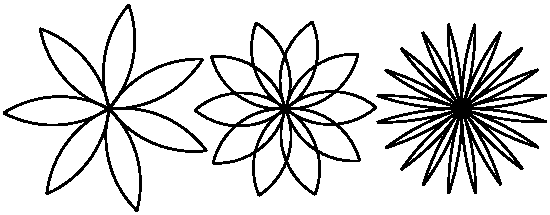
\includegraphics[scale=0.85]{../source/figs/flowers.pdf}}
\caption{Turtle flowers.}
\label{fig.flowers}
\end{figure}

\begin{exercise}
\index{flower}

%🍁% Write an appropriately general set of functions that
%🍁% can draw flowers as in Figure~\ref{fig.flowers}.

编写比较通用的一个可以画出像图4-1中那样花朵的函数集。

%🍁% Solution: \url{http://thinkpython2.com/code/flower.py},
%🍁% also requires \url{http://thinkpython2.com/code/polygon.py}.

\href{http://thinkpython2.com/code/flower.py}{参考答案},需要使用\href{http://thinkpython2.com/code/polygon.py}{这个模块}。

\end{exercise}



\begin{figure}
\centerline
{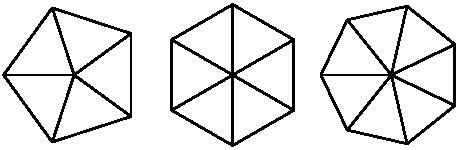
\includegraphics[scale=0.99]{../source/figs/pies.pdf}}
\caption{Turtle pies.}
\label{fig.pies}
\end{figure}


\begin{exercise}
\index{pie}

%🍁% Write an appropriately general set of functions that
%🍁% can draw shapes as in Figure~\ref{fig.pies}.

编写比较通用的一个可以画出图~{\em \ref{fig.flowers} }中那样图形的函数集。

%🍁% Solution: \url{http://thinkpython2.com/code/pie.py}.

\href{http://thinkpython2.com/code/pie.py}{参考答案}

\end{exercise}


\begin{exercise}
\index{alphabet}  \index{turtle typewriter}  \index{typewriter, turtle}

%🍁% The letters of the alphabet can be constructed from a moderate number
%🍁% of basic elements, like vertical and horizontal lines and a few
%🍁% curves.  Design an alphabet that can be drawn with a minimal
%🍁% number of basic elements and then write functions that draw the letters.

字母表中的字母可以由少量基本元素构成,例如竖线和横线,以及一些曲线。
设计一种可用由最少的基本元素绘制出的字母表,然后编写能画出各个字母的函数。

%🍁% You should write one function for each letter, with names
%🍁% \verb"draw_a", \verb"draw_b", etc., and put your functions
%🍁% in a file named {\tt letters.py}.  You can download a
%🍁% ``turtle typewriter'' from \url{http://thinkpython2.com/code/typewriter.py}
%🍁% to help you test your code.

你应该为每个字母写一个函数,起名为 {\em \li{draw_a} } ,{\em \li{draw_b} }  等等,
然后将你的函数放在一个名为 {\em \li{letters.py} }  的文件里。
你可以从 \href{http://thinkpython2.com/code/typewriter.py}{这里}
下载一个``海龟打字员''来帮你测试代码。

%🍁% You can get a solution from \url{http://thinkpython2.com/code/letters.py};
%🍁% it also requires \url{http://thinkpython2.com/code/polygon.py}.

你可以在 \href{http://thinkpython2.com/code/letters.py}{这里}找到参考答案;这个解法还要求使用 \href{http://thinkpython2.com/code/polygon.py}{这个模块} 。

\end{exercise}


\begin{exercise}

%🍁% Read about spirals at \url{http://en.wikipedia.org/wiki/Spiral}; then
%🍁% write a program that draws an Archimedian spiral (or one of the other
%🍁% kinds).  Solution: \url{http://thinkpython2.com/code/spiral.py}.

阅读关于 \href{https://zh.wikipedia.org/wiki/%E8%9E%BA%E7%BA%BF}{螺线} {\em (\href{http://en.wikipedia.org/wiki/Spiral}{spiral})} 的相关知识;
然后编写一个绘制阿基米德螺线(或者其他种类的螺线)的程序。
\index{spiral}  \index{Archimedian spiral}

\href{http://thinkpython2.com/code/spiral.py}{参考答案}

\end{exercise}

% SEIKA
% 23 Mar 2016
% 09 Jul 2016




% \chapter{Conditionals and recursion  |  条件和递归}
\chapter{条件和递归}


%🍁% The main topic of this chapter is the {\tt if} statement, which executes different code depending on the state of the program. But first I want to introduce two new operators: floor division and modulus.

本章中心议题是根据程序的状态执行不同命令的 if 语句。 在这之前我们先介绍两个新的运算符 : {\em 地板除法} (floor division) \footnote{译注:向下取整的除法。} 和{\em 求余} (modulus) 。

% \section{Floor division and modulus  |  地板除法和求余}
\section{地板除法和求余}

%🍁% The {\bf floor division} operator, \verb"//", divides two numbers and rounds down to an integer.  For example, suppose the run time of a movie is 105 minutes.  You might want to know how long that is in hours.  Conventional division returns a floating-point number:

{\em 地板除运算符} (floor division operator)为 \li{//} 即先做除法,然后将结果向下保留到整数。 例如,如果一部电影时长105 分钟,你可能想知道这代表着多少小时。 传统的除法操作会返回一个浮点数:

\begin{lstlisting}
>>> minutes = 105
>>> minutes / 60
1.75
\end{lstlisting}

%🍁% But we don't normally write hours with decimal points.  Floor division returns the integer number of hours, dropping the fraction part:

但是,以小时做单位时我们通常不会写出小数部分。地板除法丢弃除法运算结果的小数部分,返回整数个小时:

\begin{lstlisting}
>>> minutes = 105
>>> hours = minutes // 60
>>> hours
1
\end{lstlisting}

%🍁% To get the remainder, you could subtract off one hour in minutes:

如果你希望得到余数,你可以从除数中减去一个小时也就是 60 分钟:

\begin{lstlisting}
>>> remainder = minutes - hours * 60
>>> remainder
45
\end{lstlisting}

\index{floor division}  \index{floating-point division}
\index{division!floor}  \index{division!floating-point}
\index{modulus operator}  \index{operator!modulus}
\index{地板除法}  \index{浮点除法}
\index{除法!地板除}  \index{除法!浮点}
\index{求余操作符}  \index{操作符!求余}


%🍁% An alternative is to use the {\bf modulus operator}, \verb"%", which divides two numbers and returns the remainder.

另一个方法就是使用 {\em 求余运算符} (modulus operator), \li{%} ,它会将两个数相除,返回余数。


\begin{lstlisting}
>>> remainder = minutes % 60
>>> remainder
45
\end{lstlisting}

%
%🍁% The modulus operator is more useful than it seems.  For example, you can check whether one number is divisible by another---if {\tt x \% y} is zero, then {\tt x} is divisible by {\tt y}.

求余运算符比看起来更加有用。例如,你可以查看一个数是否可以被另一个数整除——如果 \li{x % y} 的结果是 $0$,那么 \li{x} 能被 \li{y} 整除。
\index{divisibility}

%🍁% Also, you can extract the right-most digit or digits from a number.  For example, {\tt x \% 10} yields the right-most digit of {\tt x} (in base 10).  Similarly {\tt x \% 100} yields the last two digits.

此外,你也能获得一个数的最右边一位或多位的数字。 例如, \li{x % 10} 返回 \li{x} 最右边一位的数字(十进制)。 类似地,\li{x % 100} 返回最后两位数字。

%🍁% If you are using Python 2, division works differently.  The division operator, \verb"/", performs floor division if both operands are integers, and floating-point division if either operand is a {\tt float}.

如果你正在使用 Python 2, 那么除法就会和前面的介绍有点不同。除法运算符 \li{/} 在被除数和除数都是整数的时候,会进行地板除,但是当被除数和除数中任意一个是浮点数的时候,则进行浮点数除法。\footnote{译注:在 Python3 中,无论任何类型都会保持小数部分。}
\index{Python 2}


% \section{Boolean expressions  |  布尔表达式}
\section{布尔表达式}
\index{boolean expression}  \index{expression!boolean}
\index{logical operator}  \index{operator!logical}

\index{布尔表达式}  \index{表达式!布尔}
\index{逻辑操作符}  \index{操作符!逻辑}

%🍁% A {\bf boolean expression} is an expression that is either true or false.  The following examples use the operator {\tt ==}, which compares two operands and produces {\tt True} if they are equal and {\tt False} otherwise:

{\em 布尔表达式} (boolean expression) 的结果要么为{\bf 真}要么为{\bf 假}。
下面的例子使用 \li{==} 运算符。 它比较两个运算数,
如果它们相等,则结果为 \li{True} ,否则结果为 \li{False} 。

\begin{lstlisting}
>>> 5 == 5
True
>>> 5 == 6
False
\end{lstlisting}

%
%🍁% {\tt True} and {\tt False} are special values that belong to the type {\tt bool}; they are not strings:

\li{True} 和 \li{False} 是属于 bool 类型的特殊值; 它们不是字符串。

\index{True special value}  \index{False special value}
\index{special value!True}  \index{special value!False}
\index{bool type}  \index{type!bool}
\index{真特殊值}  \index{假特殊值}
\index{特殊值!真}  \index{特殊值!假}
\index{bool 类型}  \index{类型!bool}



\begin{lstlisting}
>>> type(True)
<class 'bool'>
>>> type(False)
<class 'bool'>
\end{lstlisting}

%
%🍁% The {\tt ==} operator is one of the {\bf relational operators}; the others are:

\li{==} 运算符是 {\em 关系运算符} (relational operators) 之一; 其他关系运算符还有:


\begin{lstlisting}
      x != y               # x is not equal to y
      x > y                # x is greater than y
      x < y                # x is less than y
      x >= y               # x is greater than or equal to y
      x <= y               # x is less than or equal to y
\end{lstlisting}

%
%🍁% Although these operations are probably familiar to you, the Python symbols are different from the mathematical symbols.  A common error is to use a single equal sign ({\tt =}) instead of a double equal sign ({\tt ==}).  Remember that {\tt =} is an assignment operator and {\tt ==} is a relational operator.   There is no such thing as {\tt =<} or {\tt =>}.

虽然这些运算符对你来说可能很熟悉,但是 Python 的符号与数学符号不相同。
一个常见的错误是使用单独一个等号 (\li{=}) 而不是双等号 (\li{==})。
请记住, \li{=} 是赋值运算符, \li{==} 是关系运算符。 没有类似 \li{=<} 或 \li{=>} 的东西。

\index{relational operator}  \index{operator!relational}
\index{关系型运算符}  \index{运算符!关系型}

\section {Logical operators  |  逻辑运算符}
\index{logical operator}  \index{operator!logical}

%🍁% There are three {\bf logical operators}: {\tt and}, {\tt or}, and {\tt not}.  The semantics (meaning) of these operators is similar to their meaning in English.  For example, {\tt x > 0 and x < 10} is true only if {\tt x} is greater than 0 {\em and} less than 10.

有三个 {\em 逻辑运算符} (logical operators) : \li{and} 、 \li {or} 和 \li {not}。
这些运算符的含义和它们在英语的意思相似。例如, \li{x > 0 and x < 10} 只在 \li{x} 大于 \li{0} {\bf 并且} 小于 \li{10} 时为真。


\index{and operator}  \index{or operator}
\index{not operator}  \index{operator!and}
\index{operator!or}  \index{operator!not}

%🍁% {\tt n\%2 == 0 or n\%3 == 0} is true if {\em either or both} of the conditions is true, that is, if the number is divisible by 2 {\em or} 3.

\li{n%2 == 0 or n%3 == 0} 中如果 {\em 一个或两个} 条件为真,那么整个表达式即为真。也就是说,如果数字\li{n} 能被 \li{2} {\em 或者} \li{3} 整除,则为真。

%🍁% Finally, the {\tt not} operator negates a boolean expression, so {\tt not (x > y)} is true if {\tt x > y} is false, that is, if {\tt x} is less than or equal to {\tt y}.

最后,\li{not} 运算符对一个布尔表达式取反, 因此,如果 \li{x > y} 为假,也就是说 \li{x} 小于或等于 \li{y}, 则 \li{not (x > y)} 为真。

%🍁% Strictly speaking, the operands of the logical operators should be boolean expressions, but Python is not very strict. Any nonzero number is interpreted as {\tt True}:

严格来讲,逻辑运算符的运算数应该是布尔表达式,
但是Python并不严格要求。任何非0的数字都被解释成为真 ( \li{True} )。

\begin{lstlisting}
>>> 42 and True
True
\end{lstlisting}

%
%🍁% This flexibility can be useful, but there are some subtleties to it that might be confusing.  You might want to avoid it (unless you know what you are doing).

这种灵活性很有用,但有一些细节可能容易令人困惑。你可能需要避免这种用法(除非你知道你正在做什么)。


% \section{Conditional execution  |  有条件执行}
\section{有条件执行}
\label{conditional.execution}

\index{conditional statement}  \index{statement!conditional}
\index{if statement}  \index{statement!if}
\index{conditional execution}

%🍁% In order to write useful programs, we almost always need the ability to check conditions and change the behavior of the program accordingly.  {\bf Conditional statements} give us this ability.  The simplest form is the {\tt if} statement:

为了写出有用的程序,我们几乎总是需要能够检测条件,并相应地改变程序行为。
{\em 条件语句} (Conditional statements) 给予了我们这一能力。
最简单的形式是 \li{if} 语句:

\begin{lstlisting}
if x > 0:
    print('x is positive')
\end{lstlisting}

%
%🍁% The boolean expression after {\tt if} is called the {\bf condition}.  If it is true, the indented statement runs.  If not, nothing happens.

\li{if} 之后的布尔表达式被称作 {\em 条件} (condition) 。
如果它为真,则缩进的语句会被执行。 如果不是,则什么也不会发生。
\index{condition}  \index{compound statement}
\index{statement!compound}

%🍁% {\tt if} statements have the same structure as function definitions: a header followed by an indented body.  Statements like this are called {\bf compound statements}.

\li{if} 语句和函数定义有相同的结构:一个语句头跟着一个缩进的语句体。
类似的语句被称作 {\em 复合语句} (compound statements) 。

%🍁% There is no limit on the number of statements that can appear in
%🍁% the body, but there has to be at least one.
%🍁% Occasionally, it is useful to have a body with no statements (usually
%🍁% as a place keeper for code you haven't written yet).  In that
%🍁% case, you can use the {\tt pass} statement, which does nothing.

语句体中可出现的语句数目没有限制,但是至少得有一个。
有时候,一条语句都没有的语句体也是有用的(通常是为你还没写的代码占一个位子)。
这种情况下,你可以使用 \li{pass} 语句,它什么也不做。
\index{pass statement}  \index{statement!pass}


\begin{lstlisting}
if x < 0:
    pass          # TODO: need to handle negative values!
\end{lstlisting}
%

% \section{Alternative execution  |  二选一执行}
\section{二选一执行}
\label{alternative.execution}
\index{alternative execution}  \index{else keyword}  \index{keyword!else}

A second form of the {\tt if} statement is ``alternative execution'',
in which there are two possibilities and the condition determines
which one runs.  The syntax looks like this:

\li{if} 语句的第二种形式是 {\em ``二选一执行''} (alternative execution) ,
此时有两个可能的选择,由条件决定执行哪一个。 语法看起来是这样:


\begin{lstlisting}
if x % 2 == 0:
    print('x is even')
else:
    print('x is odd')
\end{lstlisting}

%
%🍁% If the remainder when {\tt x} is divided by 2 is 0, then we know that
%🍁% {\tt x} is even, and the program displays an appropriate message.  If
%🍁% the condition is false, the second set of statements runs.
%🍁% Since the condition must be true or false, exactly one of the
%🍁% alternatives will run.  The alternatives are called {\bf
%🍁%   branches}, because they are branches in the flow of execution.

如果 \li{x} 除以 \li{2} 的余数是 \li{0},那么我们知道 \li{x} 是偶数,
然后程序会打印相应的信息。 如果条件为假,则执行第二部分语句。
由于条件要么为真要么为假,两个选择中只有一个会被执行。
这些选择被称作\ **分支(branches)**\ ,因为它们是执行流程的分支。

\index{branch}  \index{分支}


% \section{Chained conditionals  |  链式条件}
\section{链式条件}

\index{chained conditional}  \index{conditional!chained}
\index{链式条件}  \index{条件!链式}

%🍁% Sometimes there are more than two possibilities and we need more than
%🍁% two branches.  One way to express a computation like that is a {\bf
%🍁% chained conditional}:

有时有超过两个可能的情况,于是我们需要多于两个的分支。
表示像这样的计算的方法之一是{\em 链式条件} (chained conditional):

\begin{lstlisting}
if x < y:
    print('x is less than y')
elif x > y:
    print('x is greater than y')
else:
    print('x and y are equal')
\end{lstlisting}

%
%🍁% {\tt elif} is an abbreviation of ``else if''.  Again, exactly one
%🍁% branch will run.  There is no limit on the number of {\tt
%🍁% elif} statements.  If there is an {\tt else} clause, it has to be
%🍁% at the end, but there doesn't have to be one.

\li{elif} 是 ``else if''的缩写。 同样地,这里只有一个分支会被执行。
\li{elif} 语句的数目没有限制。如果有一个 \li{else} 从句,
它必须是在最后,但这个语句并不是必须。
\index{elif keyword}  \index{keyword!elif}

\begin{lstlisting}
if choice == 'a':
    draw_a()
elif choice == 'b':
    draw_b()
elif choice == 'c':
    draw_c()
\end{lstlisting}

%
%🍁% Each condition is checked in order.  If the first is false,
%🍁% the next is checked, and so on.  If one of them is
%🍁% true, the corresponding branch runs and the statement
%🍁% ends.  Even if more than one condition is true, only the
%🍁% first true branch runs.

程序将按顺序逐个检测条件,如果第一个为假,则检测下一个,以此类推。
如果它们中有一个为真,相应的分支被执行,并且结束语句。
即便有不止一个条件为真,也只执行第一个为真的分支。

% \section{Nested conditionals  |  嵌套条件}
\section{嵌套条件}

\index{nested conditional}  \index{conditional!nested}

%🍁% One conditional can also be nested within another.  We could have
%🍁% written the example in the previous section like this:

一个条件可以嵌到另一个里面。我们可以这样写前一节的例子:

\begin{lstlisting}
if x == y:
    print('x and y are equal')
else:
    if x < y:
        print('x is less than y')
    else:
        print('x is greater than y')
\end{lstlisting}

%
%🍁% The outer conditional contains two branches.  The
%🍁% first branch contains a simple statement.  The second branch
%🍁% contains another {\tt if} statement, which has two branches of its
%🍁% own.  Those two branches are both simple statements,
%🍁% although they could have been conditional statements as well.

外层的条件 (outer conditional) 包含两条分支。 第一个分支包括一条简单的语句。
第二个分支包括一个 \li{if} 语句,它又有两条子分支。
这两条子分支都是简单的语句,当然它们也可以再嵌入条件语句。


%🍁% Although the indentation of the statements makes the structure apparent, {\bf nested conditionals} become difficult to read very quickly.  It is a good idea to avoid them when you can.

虽然语句的缩进使得结构很明显,但是仍然很难快速地阅读 {\em 嵌套条件} (nested conditionals) 。当你可以的时候,避免使用嵌套条件是个好办法。

%🍁% Logical operators often provide a way to simplify nested conditional statements.  For example, we can rewrite the following code using a single conditional:

逻辑运算符通常是一个简化嵌套条件语句的方法。
例如,我们可以用一个单一条件重写下面的代码:

\begin{lstlisting}
if 0 < x:
    if x < 10:
        print('x is a positive single-digit number.')
\end{lstlisting}

%
%🍁%  The {\tt print} statement runs only if we make it past both conditionals, so we can get the same effect with the {\tt and} operator:

只有通过了两个条件检测的时候, \li{print} 语句才被执行,
因此我们可以用 \li{and} 运算符得到相同的效果:


\begin{lstlisting}
if 0 < x and x < 10:
    print('x is a positive single-digit number.')
\end{lstlisting}

%🍁% For this kind of condition, Python provides a more concise option:

对于这样的条件,Python 提供了一种更加简洁的写法。

\begin{lstlisting}
if 0 < x < 10:
    print('x is a positive single-digit number.')
\end{lstlisting}


% \section{Recursion  |  递归}
\section{递归}
\label{recursion}
\index{recursion}  \index{递归}

%🍁% It is legal for one function to call another; it is also legal for a function to call itself.  It may not be obvious why that is a good thing, but it turns out to be one of the most magical things a program can do. For example, look at the following function:

一个函数调用另一个是合法的; 一个函数调用它自己其实也是合法的。
这样做的好处也许看上去不那么明显,但它实际上它是程序最神奇的魔法之一。
例如,下面这个函数:

\begin{lstlisting}
def countdown(n):
    if n <= 0:
        print('Blastoff!')
    else:
        print(n)
        countdown(n-1)
\end{lstlisting}

%
%🍁% If {\tt n} is 0 or negative, it outputs the word, ``Blastoff!'' Otherwise, it outputs {\tt n} and then calls a function named {\tt countdown}---itself---passing {\tt n-1} as an argument.

如果 \li{n} 是 0 或负数,程序输出单词 ``Blastoff!''。
否则,它输出n然后调用一个名为 \li{countdown} 的函数—即它自己 --- 传递 \li{n-1} 作为实参。

%🍁% What happens if we call this function like this?

如果我们像这样调用该函数会发生什么呢?


\begin{lstlisting}
>>> countdown(3)
\end{lstlisting}

%
%🍁% The execution of {\tt countdown} begins with {\tt n=3}, and since
%🍁% {\tt n} is greater than 0, it outputs the value 3, and then calls itself...
%🍁%
%🍁% \begin{quote}
%🍁% The execution of {\tt countdown} begins with {\tt n=2}, and since
%🍁% {\tt n} is greater than 0, it outputs the value 2, and then calls itself...
%🍁%
%🍁% \begin{quote}
%🍁% The execution of {\tt countdown} begins with {\tt n=1}, and since
%🍁% {\tt n} is greater than 0, it outputs the value 1, and then calls itself...
%🍁%
%🍁% \begin{quote}
%🍁% The execution of {\tt countdown} begins with {\tt n=0}, and since {\tt
%🍁% n} is not greater than 0, it outputs the word, ``Blastoff!'' and then
%🍁% returns.
%🍁% \end{quote}
%🍁%
%🍁% The {\tt countdown} that got {\tt n=1} returns.
%🍁% \end{quote}
%🍁%
%🍁% The {\tt countdown} that got {\tt n=2} returns.
%🍁% \end{quote}
%🍁%
%🍁% The {\tt countdown} that got {\tt n=3} returns.
%🍁%
%🍁% And then you're back in \verb"__main__".  So, the
%🍁% total output looks like this:

\newpage
\li{countdown} 开始以 \li{n=3} 执行,由于 \li{n} 大于 0, 它输出值 3,然后调用它自己...

\begin{quote}
\li{countdown} 开始以 \li{n=2} 执行,由于 \li{n} 大于 0, 它输出值 2,然后调用它自己...

\begin{quote}
\li{countdown} 开始以 \li{n=1} 执行,既然 \li{n} 大于 0,它输出值 1,然后调用它自己...

\begin{quote}
\li{countdown} 开始以 \li{n=0} 执行,由于 \li{n} 不大于 0, 它输出单词 ``Blastoff!'',然后返回。
\end{quote}

获得 \li{n=1} 的 \li{countdown} 返回。
\end{quote}

获得 \li{n=2} 的 \li{countdown} 返回。
\end{quote}

获得 \li{n=3} 的 \li{countdown} 返回。

\vspace{0.1 in}

然后回到 \li{__main__} 中。 因此整个输出类似于:

\begin{lstlisting}
3
2
1
Blastoff!
\end{lstlisting}

%
%🍁% A function that calls itself is {\bf recursive}; the process of executing it is called {\bf recursion}.

一个调用它自己的函数被称为 {\em 递归的} (recursive) ;
这种过程被称作 {\em 递归} (recursion) 。

\index{recursion}  \index{function!recursive}
\index{递归}  \index{函数!递归}

%🍁% As another example, we can write a function that prints a string {\tt n} times.

再举一例,我们可以写一个函数,其打印一个字符串 \li{n} 次。

\begin{lstlisting}
def print_n(s, n):
    if n <= 0:
        return
    print(s)
    print_n(s, n-1)
\end{lstlisting}

%
%🍁% If {\tt n <= 0} the {\bf return statement} exits the function.  The flow of execution immediately returns to the caller, and the remaining lines of the function don't run.

如果 \li{n <= 0} ,\li{return}{\em 语句} 退出函数。
执行流程马上返回到调用者,剩下的语句不会被执行。
\index{return statement}  \index{statement!return}

%🍁% The rest of the function is similar to {\tt countdown}: it displays {\tt s} and then calls itself to display {\tt s} $n-1$ additional times.  So the number of lines of output is {\tt 1 + (n - 1)}, which adds up to {\tt n}.

函数的其余部分和 \li{countdown} 相似: 它打印 \li{s} 的值,然后调用自身打印 \li{s} $n-1$ 次。 因此,输出的行数是 \li{1 + (n - 1)} ,加起来是 \li{n}。

%🍁% For simple examples like this, it is probably easier to use a {\tt for} loop.  But we will see examples later that are hard to write with a {\tt for} loop and easy to write with recursion, so it is good to start early.

对于像这样简单的例子,使用for循环可能更容易。
但是我们后面将看到一些用for循环很难写,用递归却很容易的例子,
所以早点儿开始学习递归有好处。

\index{for loop}  \index{loop!for}
\index{for 循环}  \index{循环!for}

% \section{Stack diagrams for recursive functions  |  递归函数的堆栈图}
\section{递归函数的堆栈图}
\label{recursive.stack}

\index{stack diagram}  \index{function frame}  \index{frame}
\index{堆栈图}  \index{function frame}  \index{frame}


%🍁% In Section~\ref{stackdiagram}, we used a stack diagram to represent the state of a program during a function call.  The same kind of diagram can help interpret a recursive function.

在~\ref{stackdiagram}~小节中,我们用堆栈图表示了一个函数调用期间程序的状态。
这种图也能帮我们理解递归函数。

%🍁% Every time a function gets called, Python creates a frame to contain the function's local variables and parameters. For a recursive function, there might be more than one frame on the stack at the same time.

每当一个函数被调用时,Python 生成一个新的栈帧,用于保存函数的局部变量和形参。
对于一个递归函数,在堆栈上可能同时有多个栈帧。

%🍁% Figure~\ref{fig.stack2} shows a stack diagram for {\tt countdown} called with {\tt n = 3}.

图~\ref{fig.stack2} 展示了一个以 \li{n = 3} 调用 \li{countdown} 的堆栈图。

\begin{figure}
\centerline
{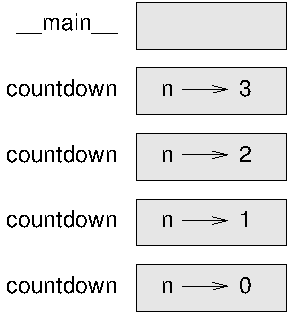
\includegraphics[scale=0.8]{../source/figs/stack2.pdf}}
%🍁% \caption{Stack diagram.}
\caption{堆栈图。}
\label{fig.stack2}
\end{figure}

%🍁% As usual, the top of the stack is the frame for \verb"__main__". It is empty because we did not create any variables in \verb"__main__" or pass any arguments to it.

\index{base case}  \index{recursion!base case}

通常,堆栈的顶部是 \li{__main__} 栈帧。
因为我们在 \li{__main__} 中没有创建任何变量,也没有传递任何实参给它,所以它是空的。

%🍁% The four {\tt countdown} frames have different values for the parameter {\tt n}.  The bottom of the stack, where {\tt n=0}, is called the {\bf base case}.  It does not make a recursive call, so there are no more frames.

对于形参 \li{n} ,四个 \li{countdown} 栈帧有不同的值。 \li{n=0} 的栈底,被称作 {\em 基础情形} (base case) 。 它不再进行递归调用了,所以没有更多的栈帧了。

%🍁% As an exercise, draw a stack diagram for \verb"print_n" called with \verb"s = 'Hello'" and {\tt n=2}. Then write a function called \verb"do_n" that takes a function object and a number, {\tt n}, as arguments, and that calls the given function {\tt n} times.

接下来练习一下,请画一个以 \li{s = 'Hello'} 和 \li{n=2} 调用 \li{print_n} 的堆栈图。 写一个名为 \li{do_n} 的函数,接受一个函数对象和一个数 \li{n} 作为实参, 能够调用指定的函数 \li{n} 次。

% \section{Infinite recursion  |  无限递归}
\section{无限递归}

\index{infinite recursion}  \index{recursion!infinite}
\index{runtime error}  \index{error!runtime}  \index{traceback}

\index{无限递归}  \index{递归!无限}
\index{runtime error}  \index{error!runtime}  \index{traceback}

%🍁% If a recursion never reaches a base case, it goes on making recursive calls forever, and the program never terminates.  This is known as {\bf infinite recursion}, and it is generally not a good idea.  Here is a minimal program with an infinite recursion:

如果一个递归永不会到达基础情形,它将永远进行递归调用,
并且程序永远不会终止。这被称作 {\em 无限递归} (infinite recursion) ,
通常这不是一个好主意。下面是一个最简单的无限递归程序:

\begin{lstlisting}
def recurse():
    recurse()
\end{lstlisting}

%
%🍁% In most programming environments, a program with infinite recursion does not really run forever.  Python reports an error message when the maximum recursion depth is reached:

在大多数编程环境里,一个具有无限递归的程序并非永远不会终止。
当达到最大递归深度时,Python会报告一个错误信息:
\index{exception!RuntimeError}  \index{RuntimeError}

\begin{lstlisting}
  File "<stdin>", line 2, in recurse
  File "<stdin>", line 2, in recurse
  File "<stdin>", line 2, in recurse
                  .
                  .
                  .
  File "<stdin>", line 2, in recurse
RuntimeError: Maximum recursion depth exceeded
\end{lstlisting}

%
%🍁% This traceback is a little bigger than the one we saw in the previous chapter.  When the error occurs, there are 1000 {\tt recurse} frames on the stack!

此回溯比我们在前面章节看到的长一些。
当错误出现的时候,在堆栈上有 1000 个{\em 递归栈帧}!

%🍁% If you write encounter an infinite recursion by accident, review your function to confirm that there is a base case that does not make a recursive call.  And if there is a base case, check whether you are guaranteed to reach it.

如果你不小心遇到了无限递归,检查你的函数,确保基础情形没有继续调用递归。
同时如果确实有基础情形,请检查基础情形是不是能够出现这种情形。

% \section{Keyboard input  |  键盘输入}
\section{键盘输入}
\index{keyboard input}

%🍁% The programs we have written so far accept no input from the user. They just do the same thing every time.

到目前为止,我们所写的程序都不接受来自用户的输入。
每次它们都只是做相同的事情。

%🍁% Python provides a built-in function called {\tt input} that stops the program and waits for the user to type something.  When the user presses {\sf  Return} or {\sf Enter}, the program resumes and \verb"input" returns what the user typed as a string.  In Python 2, the same function is called \verb"raw_input".

Python 提供了一个内建函数 \li{input} ,可以暂停程序运行,并等待用户输入。
当用户按下回车键(Return or Enter),程序恢复执行,\li{input} 以字符串形式返回用户键入的内容。在 Python 2 中,这个函数的名字叫 \li{raw_input} 。

\index{Python 2}  \index{input function}  \index{function!input}

\begin{lstlisting}
>>> text = input()
What are you waiting for?
>>> text
What are you waiting for?
\end{lstlisting}

%
%🍁% Before getting input from the user, it is a good idea to print a prompt telling the user what to type.  \verb"input" can take a prompt as an argument:

在从用户那儿获得输入之前,打印一个提示告诉用户输入什么是个好办法。
\li{input} 接受提示语作为实参。
\index{prompt}

\begin{lstlisting}
>>> name = input('What...is your name?\n')
What...is your name?
Arthur, King of the Britons!
>>> name
Arthur, King of the Britons!
\end{lstlisting}

%
%🍁% The sequence \verb"\n" at the end of the prompt represents a {\bf   newline}, which is a special character that causes a line break. That's why the user's input appears below the prompt.  \index{newline}

提示语最后的 \li{\n} 表示一个 {\em 新行} (newline) ,
它是一个特别的字符,会造成换行。 这也是用户的输入出现在提示语下面的原因。

%🍁% If you expect the user to type an integer, you can try to convert the return value to {\tt int}:

如果你期望用户键入一个整型数,那么你可以试着将返回值转化为 \li{int} :

\begin{lstlisting}
>>> prompt = 'What...is the airspeed velocity of an unladen swallow?\n'
>>> speed = input(prompt)
What...is the airspeed velocity of an unladen swallow?
42
>>> int(speed)
42
\end{lstlisting}

%
%🍁% But if the user types something other than a string of digits, you get an error:

但是,如果用户输入不是数字构成的字符串,你会获得一个错误:

\begin{lstlisting}
>>> speed = input(prompt)
What...is the airspeed velocity of an unladen swallow?
What do you mean, an African or a European swallow?
>>> int(speed)
ValueError: invalid literal for int() with base 10
\end{lstlisting}

%
%🍁% We will see how to handle this kind of error later.

我们后面将介绍处理这类错误的方法。
\index{ValueError}  \index{exception!ValueError}


% \section{Debugging  |  调试}
\section{调试}
\label{whitespace}

\index{debugging}  \index{traceback}
\index{调试}  \index{traceback}

%🍁% When a syntax or runtime error occurs, the error message contains a lot of information, but it can be overwhelming.  The most useful parts are usually:

当出现语法错误和运行时错误的时候,错误信息中会包含了很多的信息,但是信息量有可能太大。通常,最有用的部分是:

%🍁% \begin{itemize}
%🍁%
%🍁% \item What kind of error it was, and
%🍁%
%🍁% \item Where it occurred.
%🍁%
%🍁% \end{itemize}

\begin{itemize}

\item 是哪类错误,以及

\item 在哪儿出现。

\end{itemize}

%🍁% Syntax errors are usually easy to find, but there are a few gotchas.  Whitespace errors can be tricky because spaces and tabs are invisible and we are used to ignoring them.

语法错误通常很容易被找到,但也有一些需要注意的地方。
空白分隔符错误很棘手,因为空格和制表符是不可见的,而且我们习惯于忽略它们。
\index{whitespace}
\index{空白分隔符}

\begin{lstlisting}
>>> x = 5
>>>  y = 6
  File "<stdin>", line 1
    y = 6
    ^
IndentationError: unexpected indent
\end{lstlisting}

%
%🍁% In this example, the problem is that the second line is indented by one space.  But the error message points to {\tt y}, which is misleading.  In general, error messages indicate where the problem was discovered, but the actual error might be earlier in the code, sometimes on a previous line.

在这个例子中,问题在于第二行缩进了一个空格。
但是错误信息指向y,这是个误导。 通常,错误信息指向发现错误的地方,
但是实际的错误可能发生在代码中更早的地方, 有时在前一行。
\index{error!runtime}  \index{runtime error}

%🍁% The same is true of runtime errors.  Suppose you are trying to compute a signal-to-noise ratio in decibels.  The formula is $SNR_{db} = 10 \log_{10} (P_{signal} / P_{noise})$.  In Python, you might write something like this:

运行时错误也同样存在这个问题。假设你正试图计算分贝信噪比。
公式是 $SNR_{db} = 10 \log_{10} (P_{signal} / P_{noise})$ 。
在 Python 中,你可能会写出这样的代码:

\begin{lstlisting}
import math
signal_power = 9
noise_power = 10
ratio = signal_power // noise_power
decibels = 10 * math.log10(ratio)
print(decibels)
\end{lstlisting}

%
%🍁% When you run this program, you get an exception:

但是,当你运行它的时候, 你却获得一个异常。

%
\index{exception!OverflowError}  \index{OverflowError}

\begin{lstlisting}
Traceback (most recent call last):
  File "snr.py", line 5, in ?
    decibels = 10 * math.log10(ratio)
ValueError: math domain error
\end{lstlisting}

%
%🍁% The error message indicates line 5, but there is nothing wrong with that line.  To find the real error, it might be useful to print the value of {\tt ratio}, which turns out to be 0.  The problem is in line 4, which uses floor division instead of floating-point division.

该错误信息指向第 5 行,但是那一行没什么错误。
为了找到真正的错误,打印 \li{ratio} 的值也许会有用,结果发现它实际上是 0。
那么问题是在第 4 行,使用了地板除而不是浮点数除法。
\index{floor division}  \index{division!floor}

%🍁% You should take the time to read error messages carefully, but don't assume that everything they say is correct.

你需要花些时间仔细阅读错误信息,但不要轻易地相信错误信息的提示都是准确的。

% \section{Glossary  |  术语表}
\section{术语表}

\begin{description}

%🍁% \item[floor division:] An operator, denoted {\tt //}, that divides two numbers and rounds down (toward zero) to an integer.
%🍁% \index{floor division}
%🍁% \index{division!floor}

\item[地板除法:] 一个操作符,用 \li{//} 表示,表示对两个数做除法同时向 0 取整。
\index{floor division}  \index{division!floor}

%🍁% \item[modulus operator:]  An operator, denoted with a percent sign ({\tt \%}), that works on integers and returns the remainder when one number is divided by another.
%🍁% \index{modulus operator}  \index{operator!modulus}

\item[求余运算符:] 一个运算符,用百分号 \li{%} 表示,返回两个数相除的余数。
\index{modulus operator}  \index{operator!modulus}

%🍁% \item[boolean expression:] An expression whose value is either {\tt True} or {\tt False}.
%🍁% \index{boolean expression}  \index{expression!boolean}

\item[布尔表达式:] 一个值要么为真要么为假的表达式。
\index{boolean expression}  \index{expression!boolean}

%🍁% \item[relational operator:] One of the operators that compares
%🍁% its operands: {\tt ==}, {\tt !=}, {\tt >}, {\tt <}, {\tt >=}, and {\tt <=}.

\item[关系运算符:] 对其运算符进行比较的运算符: \li{==},\li{!=},\li{>},\li{<},\li{>=},\li{<=}。

%🍁% \item[logical operator:] One of the operators that combines boolean expressions: {\tt and}, {\tt or}, and {\tt not}.

\item[逻辑运算符:] 将布尔表达式组合在一起的运算符: \li{and}, \li{or},和 \li{not}。

%🍁% \item[conditional statement:]  A statement that controls the flow of execution depending on some condition.
%🍁% \index{conditional statement}  \index{statement!conditional}

\item[条件语句:] 一段根据某个条件决定程序执行流程的语句。
\index{conditional statement}  \index{statement!conditional}

%🍁% \item[condition:] The boolean expression in a conditional statement that determines which branch runs.
%🍁% \index{condition}

\item[条件:] 决定哪个分支会被执行的布尔表达式。
\index{condition}

%🍁% \item[compound statement:]  A statement that consists of a header and a body.  The header ends with a colon (:).  The body is indented relative to the header.
%🍁% \index{compound statement}

\item[复合语句:] 由语句头和语句体组成的语句。语句头以 : 结尾,语句体相对语句头缩进。
\index{compound statement}

%🍁% \item[branch:] One of the alternative sequences of statements in a conditional statement.
%🍁% \index{branch}

\item[分支:] 条件语句中的选择性语句序列。
\index{branch}

%🍁% \item[chained conditional:]  A conditional statement with a series of alternative branches.
%🍁% \index{chained conditional}  \index{conditional!chained}

\item[链式条件:] 由一系列替代分支组成的条件语句。
\index{chained conditional}  \index{conditional!chained}

%🍁% \item[nested conditional:]  A conditional statement that appears in one of the branches of another conditional statement.
%🍁% \index{nested conditional}  \index{conditional!nested}

\item[嵌套条件:] 出现另一个条件语句某个分支中的条件语句。
\index{nested conditional}  \index{conditional!nested}

%🍁% \item[return statement:] A statement that causes a function to end immediately and return to the caller.

\item[返回语句:] 结束函数执行并且将结果返回给调用者的语句。

%🍁% \item[recursion:]  The process of calling the function that is currently executing.
%🍁% \index{recursion}

\item[递归:] 调用正在执行的函数本身的过程。
\index{recursion}

%🍁% \item[base case:]  A conditional branch in a recursive function that does not make a recursive call.
%🍁% \index{base case}

\item[基本情形:] 在递归函数中,不进行递归调用的条件分支。
\index{base case}

%🍁% \item[infinite recursion:]  A recursion that doesn't have a base case, or never reaches it.  Eventually, an infinite recursion causes a runtime error.
%🍁% \index{infinite recursion}

\item[无限递归:] 没有基本情形或者无法出现基本情形的递归函数。最终无限递归会导致运行时错误。
\index{infinite recursion}

\end{description}

% \section{Exercises  |  练习}
\section{练习}

\begin{exercise}

%🍁% The {\tt time} module provides a function, also named {\tt time}, that returns the current Greenwich Mean Time in ``the epoch'', which is an arbitrary time used as a reference point.  On UNIX systems, the epoch is 1 January 1970.

{\em \li{time}} 模块提供了一个可以返回当前格林威治标准时间的函数,名字也是 {\em time}。这里的格林威治标准时间用纪元 ({\em ``the epoch''}) 以来的秒数表示,
纪元是一个任意的参考点。在 {\em Unix} 系统中,纪元是{\em 1970}年{\em 1}月{\em 1}日。

\begin{em}
\begin{lstlisting}
>>> import time
>>> time.time()
1437746094.5735958
\end{lstlisting}
\end{em}

%🍁% Write a script that reads the current time and converts it to a time of day in hours, minutes, and seconds, plus the number of days since the epoch.

请写一个脚本读取当前时间,并且将其转换为纪元以来经过了多少天、小时、分钟和秒。

\end{exercise}


\begin{exercise}
\index{Fermat's Last Theorem}

%🍁% Fermat's Last Theorem says that there are no positive integers $a$, $b$, and $c$ such that

%🍁% \[ a^n + b^n = c^n \]

%
%🍁% for any values of $n$ greater than 2.

费马大定理 {\em (Fermat’s Last Theorem)}称,没有任何整型数 $a$、 $b$ 和 $c$ 能够使:

\[ a^n + b^n = c^n \]

对于任何大于 2 的 $n$ 成立。

\begin{enumerate}

%🍁% \item Write a function named \verb"check_fermat" that takes four parameters---{\tt a}, {\tt b}, {\tt c} and {\tt n}---and checks to see if Fermat's theorem holds.  If $n$ is greater than 2 and

%🍁% \[a^n + b^n = c^n \]

%
%🍁% the program should print, ``Holy smokes, Fermat was wrong!'' Otherwise the program should print, ``No, that doesn't work.''

\item 写一个名为 {\em \li{check_fermat}} 的函数,接受四个形参 --- {\em \li{a}}, {\em \li{b}}, {\em \li{c}} 以及 {\em \li{n}} --- 检查费马大定理是否成立。 如果 {\em $n$} 大于 2 且 等式

\[a^n + b^n = c^n \]

成立,程序应输出 {\em ``Holy smokes, Fermat was wrong!''}。  否则程序应输出 {\em ``No, that doesn’t work.''}。

%🍁% \item Write a function that prompts the user to input values  for {\tt a}, {\tt b}, {\tt c} and {\tt n}, converts them to integers, and uses \verb"check_fermat" to check whether they violate Fermat's theorem.

\item 写一个函数提示用户输入 {\em \li{a}}, {\em \li{b}}, {\em \li{c}}以及 {\em \li{n}} 的值,将它们转换成整型数, 然后使用 {\em \li{check_fermat}} 检查他们是否会违反了费马大定理。

\end{enumerate}

\end{exercise}


\begin{exercise}
\index{triangle}

%🍁% If you are given three sticks, you may or may not be able to arrange them in a triangle.  For example, if one of the sticks is 12 inches long and the other two are one inch long, you will not be able to get the short sticks to meet in the middle.  For any three lengths, there is a simple test to see if it is possible to form a triangle:

如果你有三根棍子,你有可能将它们组成三角形,也可能不行。
比如,如果一根棍子是 {\em 12} 英寸长,其它两根都是 {\em 1} 英寸长,显然
你不可能让两根短的在中间接合。对于任意三个长度,有一个简单的测试
能验证它们能否组成三角形:

%🍁% \begin{quotation}
%🍁% If any of the three lengths is greater than the sum of the other   two, then you cannot form a triangle.  Otherwise, you can.  (If the sum of two lengths equals the third, they form what is called a ``degenerate'' triangle.)
%🍁% \end{quotation}

\begin{quotation}
如果三个长度中的任意一个超过了其它二者之和,就不能组成三角形。否则,可以组成。(如果两个长度之和等于第三个,它们就组成所谓 ```退化的'' 三角形。)
\end{quotation}

\begin{enumerate}

%🍁% \item Write a function named \verb"is_triangle" that takes three integers as arguments, and that prints either ``Yes'' or ``No'', depending on whether you can or cannot form a triangle from sticks with the given lengths.

\item 写一个名为 {\em \li{is_triangle}} 的函数,其接受三个整数作为形参,
   能够根据给定的三个长度的棍子能否构成三角形来打印 {\em ``Yes''} 或 {\em ``No''}。

%🍁% \item Write a function that prompts the user to input three stick lengths, converts them to integers, and uses \verb"is_triangle" to check whether sticks with the given lengths can form a triangle.

\item 写一个函数,提示用户输入三根棍子的长度,将它们转换成整型数,然后使用
   {\em \li{is_triangle}} 检查给定长度的棍子能否构成三角形。

\end{enumerate}

\end{exercise}

\begin{exercise}
%🍁% What is the output of the following program? Draw a stack diagram that shows the state of the program when it prints the result.

下面程序的输出是什么? 画出展示程序每次打印输出时的堆栈图。

\begin{em}
\begin{lstlisting}
def recurse(n, s):
    if n == 0:
        print(s)
    else:
        recurse(n-1, n+s)

recurse(3, 0)
\end{lstlisting}
\end{em}

%🍁% \begin{enumerate}

%🍁% \item What would happen if you called this function like this: {\tt recurse(-1, 0)}?

%🍁% \item Write a docstring that explains everything someone would need to know in order to use this function (and nothing else).

%🍁% \end{enumerate}

\begin{enumerate}

\item 如果你这样调用函数: {\em \li{recurse(-1,0)}} ,会有什么结果?

\item 请写一个文档字符串,解释调用该函数时需要了解的全部信息(仅此而已)。

\end{enumerate}

\end{exercise}

%🍁% The following exercises use the {\tt turtle} module, described in Chapter~\ref{turtlechap}:
\index{TurtleWorld}

后面的习题要用到第~\ref{turtlechap}章中的 \li{turtle}:

\begin{exercise}

%🍁% Read the following function and see if you can figure out what it does.  Then run it (see the examples in Chapter~\ref{turtlechap}).

阅读如下的函数,看看你能否看懂它是做什么的。然后运行它(见第\ref{turtlechap}章的例子)。

\begin{em}
\begin{lstlisting}
def draw(t, length, n):
    if n == 0:
        return
    angle = 50
    t.fd(length*n)
    t.lt(angle)
    draw(t, length, n-1)
    t.rt(2*angle)
    draw(t, length, n-1)
    t.lt(angle)
    t.bk(length*n)
\end{lstlisting}
\end{em}

\end{exercise}


\begin{figure}
\centerline
{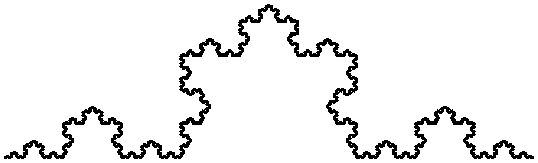
\includegraphics[scale=0.8]{../source/figs/koch.pdf}}
% \caption{A Koch curve.}
\caption{科赫曲线。}
\label{fig.koch}
\end{figure}


\begin{exercise}
\index{Koch curve}

%🍁% The Koch curve is a fractal that looks something like Figure~\ref{fig.koch}.  To draw a Koch curve with length $x$, all you have to do is

科赫曲线 {\em (Koch Curve)} 是一个看起来类似图~\ref{fig.koch}的不规则碎片几何体 {\em (fractal)}。 要画一个长度为 $x$ 的科赫曲线,你只需要:

%🍁% \begin{enumerate}
%🍁%
%🍁% \item Draw a Koch curve with length $x/3$.
%🍁%
%🍁% \item Turn left 60 degrees.
%🍁%
%🍁% \item Draw a Koch curve with length $x/3$.
%🍁%
%🍁% \item Turn right 120 degrees.
%🍁%
%🍁% \item Draw a Koch curve with length $x/3$.
%🍁%
%🍁% \item Turn left 60 degrees.
%🍁%
%🍁% \item Draw a Koch curve with length $x/3$.
%🍁%
%🍁% \end{enumerate}

\begin{enumerate}

\item 画一个长度为 $x/3$ 的科赫曲线。

\item 左转 $60$ 度。

\item 画一个长度为 $x/3$ 的科赫曲线。

\item 右转 $60$ 度。

\item 画一个长度为 $x/3$ 的科赫曲线。

\item 左转 $60$ 度。

\item 画一个长度为 $x/3$ 的科赫曲线。

\end{enumerate}

%🍁% The exception is if $x$ is less than 3: in that case, you can just draw a straight line with length $x$.

例外情况是 $x$ 小于3的情形:此时,你只需要
画一道长度为 $x$ 的直线。

%🍁% \begin{enumerate}
%🍁%
%🍁% \item Write a function called {\tt koch} that takes a turtle and
%🍁% a length as parameters, and that uses the turtle to draw a Koch
%🍁% curve with the given length.
%🍁%
%🍁% \item Write a function called {\tt snowflake} that draws three
%🍁% Koch curves to make the outline of a snowflake.
%🍁%
%🍁% Solution: \url{http://thinkpython2.com/code/koch.py}.
%🍁%
%🍁% \item The Koch curve can be generalized in several ways.  See
%🍁% \url{http://en.wikipedia.org/wiki/Koch_snowflake} for examples and
%🍁% implement your favorite.
%🍁%
%🍁% \end{enumerate}

\begin{enumerate}

\item 写一个名为 {\em \li{koch}} 的函数,接受一个海龟和一个长度作为形参,然后
   使用海龟画一条给定长度的科赫曲线。

\item 写一个名为 {\em \li{snowflake}} 的函数,画出三条科赫曲线,构成雪花的轮廓。

\href{http://thinkpython.com/code/koch.py}{参考答案}

\item 科赫曲线能够以多种方式泛化。

点击\href{http://en.wikipedia.org/wiki/Koch_snowflake}{此处}查看例子,并实现你最喜欢的那种方式。

\end{enumerate}

\end{exercise}



%🍁%
%🍁% \chapter{Fruitful functions  |  有返回值的函数}
\chapter{有返回值的函数}
\label{fruitchap}

%🍁% Many of the Python functions we have used, such as the math
%🍁% functions, produce return values.  But the functions we've written
%🍁% are all void: they have an effect, like printing a value
%🍁% or moving a turtle, but they don't have a return value.  In
%🍁% this chapter you will learn to write fruitful functions.

许多我们前面使用过的 Python 函数都会产生返回值, 如数学函数。
但目前我们所写的函数都是空函数 (void): 它们产生某种效果, 像打印一个值或是移动乌龟,但是并没有返回值。
在本章中, 你将学习如何写一个有返回值的函数。

%🍁% \section{Return values  |  返回值}
\section{返回值}
\index{return value}  \index{返回值}

%🍁% Calling the function generates a return
%🍁% value, which we usually assign to a variable or use as part of an
%🍁% expression.

调用一个有返回值的函数会生成一个返回值, 我们通常将其赋值给某个变量或是作为表达式的一部分。

\begin{lstlisting}
e = math.exp(1.0)
height = radius * math.sin(radians)
\end{lstlisting}

%
%🍁% The functions we have written so far are void.  Speaking casually,
%🍁% they have no return value; more precisely,
%🍁% their return value is {\tt None}.

目前我们所写的函数都是空函数。
泛泛地来看, 它们没有返回值; 更准确地说, 它们的返回值是 \li{None} 。

%🍁% In this chapter, we are (finally) going to write fruitful functions.
%🍁% The first example is {\tt area}, which returns the area of a circle
%🍁% with the given radius:

本章中, 我们(终于)要开始写有返回值的函数了。
第一个例子是 \li{area} , 返回给定半径圆的面积。

\begin{lstlisting}
def area(radius):
    a = math.pi * radius**2
    return a
\end{lstlisting}

%
%🍁% We have seen the {\tt return} statement before, but in a fruitful
%🍁% function the {\tt return} statement includes
%🍁% an expression.  This statement means: ``Return immediately from
%🍁% this function and use the following expression as a return value.''
%🍁% The expression can be arbitrarily complicated, so we could
%🍁% have written this function more concisely:

我们之前已经见过 \li{return} 语句,但在有返回值的函数中, \li{return} 语句包含一个表达式。
条语句的意思是:``马上从该函数返回,并使用接下来的表达式作为返回值。''
此表达式可以是任意复杂的, 因此我们可以将该函数写得更简洁些:
\index{return statement}  \index{statement!return}

\begin{lstlisting}
def area(radius):
    return math.pi * radius**2
\end{lstlisting}

%
%🍁% On the other hand, {\bf temporary variables} like {\tt a} can make
%🍁% debugging easier.

另一方面, 像 \li{a} 这样的 {\em 临时变量} (temporary variables) 能使调试变得更简单。

\index{temporary variable}  \index{variable!temporary}

%🍁% Sometimes it is useful to have multiple return statements, one in each
%🍁% branch of a conditional:

有时,在条件语句的每一个分支内各有一个返回语句会很有用:

\begin{lstlisting}
def absolute_value(x):
    if x < 0:
        return -x
    else:
        return x
\end{lstlisting}

%
%🍁% Since these {\tt return} statements are in an alternative conditional,
%🍁% only one runs.

因为这些 \li{return} 语句在不同的条件内,最后只有{\bf 一个}会被执行。

%🍁% As soon as a return statement runs, the function
%🍁% terminates without executing any subsequent statements.
%🍁% Code that appears after a {\tt return} statement, or any other place
%🍁% the flow of execution can never reach, is called {\bf dead code}.

一旦一条返回语句执行,函数则终止,不再执行后续的语句。出现在某条return语句之后的代码,或者在执行流程永远不会到达之处的代码,被称为 {\em 死代码} (dead code)。
\index{dead code}  \index{死代码}

%🍁% In a fruitful function, it is a good idea to ensure
%🍁% that every possible path through the program hits a
%🍁% {\tt return} statement.  For example:

在一个有返回值的函数中, 最好保证程序执行的每一个流程最终都会碰到一个 \li{return} 语句。例如:

\begin{lstlisting}
def absolute_value(x):
    if x < 0:
        return -x
    if x > 0:
        return x
\end{lstlisting}

%
%🍁% This function is incorrect because if {\tt x} happens to be 0,
%🍁% neither condition is true, and the function ends without hitting a
%🍁% {\tt return} statement.  If the flow of execution gets to the end
%🍁% of a function, the return value is {\tt None}, which is not
%🍁% the absolute value of 0.

这个函数是有问题的。 原因是如果 \li{x} 恰好是 0, 则没有条件为真, 函数将会在未执行任何 \li{return} 语句的情况下终止。 如果函数按照这种执行流程执行完毕,返回值将是 \li{None} ,这可不是 0 的绝对值。
\index{None special value}  \index{special value!None}

\begin{lstlisting}
>>> absolute_value(0)
None
\end{lstlisting}

%
%🍁% By the way, Python provides a built-in function called
%🍁% {\tt abs} that computes absolute values.

顺便说一下,Python提供了一个的内建函数 \li{abs} 用来计算绝对值。
\index{abs function}  \index{function!abs}

%🍁% As an exercise, write a {\tt compare} function
%🍁% takes two values, {\tt x} and {\tt y}, and returns {\tt 1} if {\tt x > y},
%🍁% {\tt 0} if {\tt x == y}, and {\tt -1} if {\tt x < y}.

我们来做个练习,写一个比较函数 \li{compare} ,接受两个值 \li{x} 和 \li{y} 。
如果 \li{x > y}, 则返回 \li{1} ;如果 \li{x == y}, 则返回 \li{0} ;如果 \li{x < y},则返回 \li{-1} 。
\index{compare function}  \index{function!compare}


%🍁% \section{Incremental development  |  增量式开发}
\section{增量式开发}
\label{incremental.development}
\index{development plan!incremental}  \index{开发计划!增量式}

%🍁% As you write larger functions, you might find yourself
%🍁% spending more time debugging.

随着你写的函数越来越大,你在调试上花的时候可能会越来越多。

%🍁% To deal with increasingly complex programs,
%🍁% you might want to try a process called
%🍁% {\bf incremental development}.  The goal of incremental development
%🍁% is to avoid long debugging sessions by adding and testing only
%🍁% a small amount of code at a time.

为了应对越来越复杂的程序,你可以开始尝试叫作 {\em 增量式开发} (incremental development) 的方法。 增量式开发的目标,是通过每次只增加和测试少量代码,来避免长时间的调试。
\index{testing!incremental development}  \index{Pythagorean theorem}
\index{测试!增量开发}

%🍁% As an example, suppose you want to find the distance between two
%🍁% points, given by the coordinates $(x_1, y_1)$ and $(x_2, y_2)$.
%🍁% By the Pythagorean theorem, the distance is:

举个例子,假设你想计算两个给定坐标点 $(x_1, y_1)$ 和 $(x_2, y_2)$ 之间的距离。根据毕达哥拉斯定理\footnote{译注:the Pythagorean theorem, 即勾股定理},二者的距离是:


\begin{displaymath}
\mathrm{distance} = \sqrt{(x_2 - x_1)^2 + (y_2 - y_1)^2}
\end{displaymath}

%
%🍁% The first step is to consider what a {\tt distance} function should
%🍁% look like in Python.  In other words, what are the inputs (parameters)
%🍁% and what is the output (return value)?

第一步要考虑的是在 Python 中,距离函数看起来会是什么样。换句话说,输入(形参)和输出(返回值)是什么?

%🍁% In this case, the inputs are two points, which you can represent
%🍁% using four numbers.  The return value is the distance represented by
%🍁% a floating-point value.

本例中,输入是可以用 4 个数表示的两个点。 返回值是距离, 用浮点数表示。

%🍁% Immediately you can write an outline of the function:

现在你就可以写出此函数的轮廓了:

\begin{lstlisting}
def distance(x1, y1, x2, y2):
    return 0.0
\end{lstlisting}

%
%🍁% Obviously, this version doesn't compute distances; it always returns
%🍁% zero.  But it is syntactically correct, and it runs, which means that
%🍁% you can test it before you make it more complicated.

显然,此版本不能计算距离;它总是返回 0 。但是在语法上它是正确的,并且能运行,这意味着你可以在使它变得更复杂之前测试它。

%🍁% To test the new function, call it with sample arguments:

用样例实参调用它来进行测试。

\begin{lstlisting}
>>> distance(1, 2, 4, 6)
0.0
\end{lstlisting}

%
%🍁% I chose these values so that the horizontal distance is 3 and the
%🍁% vertical distance is 4; that way, the result is 5, the hypotenuse
%🍁% of a 3-4-5 triangle. When testing a function, it is
%🍁% useful to know the right answer.

我选择的这些值,可以使水平距离为 3 ,垂直距离为 4 ;
这样结果自然是 5,构成了一个勾三股四弦五的直角三角形。
测试一个函数时,知道正确的答案是很有用的。
\index{testing!knowing the answer}
\index{测试!已知结果}

%🍁% At this point we have confirmed that the function is syntactically
%🍁% correct, and we can start adding code to the body.
%🍁% A reasonable next step is to find the differences
%🍁% $x_2 - x_1$ and $y_2 - y_1$.  The next version stores those values in
%🍁% temporary variables and prints them.

此时我们已经确认这个函数在语法上是正确的,我们可以开始往函数体中增加代码。
下一步合理的操作,应该是求 $x_2 - x_1$ 和 $y_2 - y_1$ 这两个差值。
下一个版本在临时变量中存储这些值并打印出来。

\begin{lstlisting}
def distance(x1, y1, x2, y2):
    dx = x2 - x1
    dy = y2 - y1
    print('dx is', dx)
    print('dy is', dy)
    return 0.0
\end{lstlisting}

%
%🍁% If the function is working, it should display \verb"dx is 3" and
%🍁% \verb"dy is 4".  If so, we know that the function is getting the right
%🍁% arguments and performing the first computation correctly.  If not,
%🍁% there are only a few lines to check.

如果这个函数正常运行,它应该显示 \li{dx is 3}  以及 \li{dy is 4} 。
这样的话我们就知道函数获得了正确的实参并且正确执行了第一步计算。
如果不是,也只要检查几行代码。

%🍁% Next we compute the sum of squares of {\tt dx} and {\tt dy}:

下一步我们计算 \li{dx} 和 \li{dy} 的平方和。

\begin{lstlisting}
def distance(x1, y1, x2, y2):
    dx = x2 - x1
    dy = y2 - y1
    dsquared = dx**2 + dy**2
    print('dsquared is: ', dsquared)
    return 0.0
\end{lstlisting}

%
%🍁% Again, you would run the program at this stage and check the output
%🍁% (which should be 25).
%🍁% Finally, you can use {\tt math.sqrt} to compute and return the result:

再一次运行程序并检查结果 (应该是 25 )。
最后,你可以使用 \li{math.sqrt} 计算并返回结果。
\index{sqrt}  \index{function!sqrt}

\begin{lstlisting}
def distance(x1, y1, x2, y2):
    dx = x2 - x1
    dy = y2 - y1
    dsquared = dx**2 + dy**2
    result = math.sqrt(dsquared)
    return result
\end{lstlisting}

%
%🍁% If that works correctly, you are done.  Otherwise, you might
%🍁% want to print the value of {\tt result} before the return
%🍁% statement.

如果其正确运行的话,你就成功了。否则你可能想在 \li{return} 语句前打印结果检查一下。

%🍁% The final version of the function doesn't display anything when it
%🍁% runs; it only returns a value.  The {\tt print} statements we wrote
%🍁% are useful for debugging, but once you get the function working, you
%🍁% should remove them.  Code like that is called {\bf scaffolding}
%🍁% because it is helpful for building the program but is not part of the
%🍁% final product.

该函数的最终版不会在运行时显示任何东西,仅仅返回一个值。
我们之前写的 \li{print} 语句在调试时是很有用的, 不过在函数能够正确运行之后, 你就该删了它们。
我们称这样的代码为 {\em 脚手架代码} (scaffolding) , 因为它对程序的构建很有用, 但不是最终产品的一部分。
\index{scaffolding}

%🍁% When you start out, you should add only a line or two of code at a
%🍁% time.  As you gain more experience, you might find yourself writing
%🍁% and debugging bigger chunks.  Either way, incremental development
%🍁% can save you a lot of debugging time.

当你刚开始的时候, 最好每次只加入一两行代码。
随着经验见长, 你会发现自己可以编写、调试更大的代码块了。
无论哪种方式, 增量式开发都能节省你大量的调试时间。

%🍁% The key aspects of the process are:

这种开发方式的关键是:


%🍁% \begin{enumerate}
%🍁% \item Start with a working program and make small incremental changes.
%🍁% At any point, if there is an error, you should have a good idea
%🍁% where it is.
%🍁%
%🍁% \item Use variables to hold intermediate values so you can
%🍁% display and check them.
%🍁%
%🍁% \item Once the program is working, you might want to remove some of
%🍁% the scaffolding or consolidate multiple statements into compound
%🍁% expressions, but only if it does not make the program difficult to
%🍁% read.
%🍁% \end{enumerate}

\begin{enumerate}
\item 从一个能运行的程序开始,并且每次只增加少量改动。无论你何时遇到错误,都能够清楚定位错误的源头。

\item 用临时变量存储中间值,这样你就能显示并检查它们。

\item 一旦程序正确运行,你要删除一些脚手架代码,或者将多条语句组成复合表达式,但是前提是不会影响程序的可读性。
\end{enumerate}

%🍁% As an exercise, use incremental development to write a function
%🍁% called {\tt hypotenuse} that returns the length of the hypotenuse of a
%🍁% right triangle given the lengths of the other two legs as arguments.
%🍁% Record each stage of the development process as you go.

我们来做个练习:运用增量开发方式,写一个叫作 \li{hypotenuse} 的函数,接受直角三角形的两直角边长作为实参,返回该三角形斜边的长度。记录下你开发过程中的每一步。
\index{hypotenuse}



%🍁% \section{Composition  |  组合}
\section{组合}
\index{composition}  \index{function composition}

%🍁% As you should expect by now, you can call one function from within
%🍁% another.  As an example, we'll write a function that takes two points,
%🍁% the center of the circle and a point on the perimeter, and computes
%🍁% the area of the circle.

你现在应该已经猜到了,你可以从一个函数内部调用另一个函数。
作为示例,我们接下来写一个函数,接受两个点为参数,分别是圆心和圆周上一点,然后计算圆的面积。

%🍁% Assume that the center point is stored in the variables {\tt xc} and
%🍁% {\tt yc}, and the perimeter point is in {\tt xp} and {\tt yp}. The
%🍁% first step is to find the radius of the circle, which is the distance
%🍁% between the two points.  We just wrote a function, {\tt
%🍁% distance}, that does that:

假设圆心坐标存储在变量 \li{xc} 和 \li{yc} 中,圆周上的点的坐标存储在 \li{xp} 和 \li{yp} 中。第一步是计算圆半径,也就是这两个点的距离。
我们刚写的 \li{distance} 函数就可以计算距离:

\begin{lstlisting}
radius = distance(xc, yc, xp, yp)
\end{lstlisting}

%
%🍁% The next step is to find the area of a circle with that radius;
%🍁% we just wrote that, too:

下一步是用得到的半径计算圆面积;我们也刚写了这样的函数:

\begin{lstlisting}
result = area(radius)
\end{lstlisting}

%
%🍁% Encapsulating these steps in a function, we get:

将这些步骤封装在一个函数中,可以得到下面的函数:
\index{encapsulation}  \index{封装}

\begin{lstlisting}
def circle_area(xc, yc, xp, yp):
    radius = distance(xc, yc, xp, yp)
    result = area(radius)
    return result
\end{lstlisting}

%
%🍁% The temporary variables {\tt radius} and {\tt result} are useful for
%🍁% development and debugging, but once the program is working, we can
%🍁% make it more concise by composing the function calls:

临时变量 \li{radius} 和 \li{result} 对于开发调试很有用的,但是
一旦函数正确运行了,我们可以通过合并函数调用,将程序变得更简洁:

\begin{lstlisting}
def circle_area(xc, yc, xp, yp):
    return area(distance(xc, yc, xp, yp))
\end{lstlisting}

%

%🍁% \section{Boolean functions  |  布尔函数}
\section{布尔函数}
\label{boolean}

%🍁% Functions can return booleans, which is often convenient for hiding
%🍁% complicated tests inside functions.  \index{boolean function}
%🍁% For example:

函数可以返回 {\em 布尔值} (booleans) , 通常对于隐藏函数内部的复杂测试代码非常方便。 例如:

\begin{lstlisting}
def is_divisible(x, y):
    if x % y == 0:
        return True
    else:
        return False
\end{lstlisting}


%🍁% It is common to give boolean functions names that sound like yes/no
%🍁% questions; \verb"is_divisible" returns either {\tt True} or {\tt False}
%🍁% to indicate whether {\tt x} is divisible by {\tt y}.

通常布尔函数名听起来像是一个疑问句,回答不是 Yes 就是 No, \li{is_divisible} 通过返回 \li{True} 或 \li{False} 来表示 \li{x} 是否可以被 \li{y} 整除。

%🍁% Here is an example:

请看下面的示例:

\begin{lstlisting}
>>> is_divisible(6, 4)
False
>>> is_divisible(6, 3)
True
\end{lstlisting}

%🍁% The result of the {\tt ==} operator is a boolean, so we can write the
%🍁% function more concisely by returning it directly:

\li{==} 运算符的结果是布尔值,因此我们直接返回它,让代码变得更简洁。

\begin{lstlisting}
def is_divisible(x, y):
    return x % y == 0
\end{lstlisting}

%
%🍁% Boolean functions are often used in conditional statements:

布尔函数通常被用于条件语句中:
\index{conditional statement}  \index{statement!conditional}

\begin{lstlisting}
if is_divisible(x, y):
    print('x is divisible by y')
\end{lstlisting}

%
%🍁% It might be tempting to write something like:

很容易写出下面这样的代码:

\begin{lstlisting}
if is_divisible(x, y) == True:
    print('x is divisible by y'
\end{lstlisting}

%
%🍁% But the extra comparison is unnecessary.

但这里的比较是多余的。

%🍁% As an exercise, write a function \verb"is_between(x, y, z)" that
%🍁% returns {\tt True} if $x \le y \le z$ or {\tt False} otherwise.

我们来做个练习:写一个函数  \li{is_between(x, y, z)} ,如果 $x \le y \le z$ 返回 \li{True} 否则返回 \li{False}。

%🍁% \section{More recursion  |  再谈递归}
\section{再谈递归}
\label{more.recursion}
\index{recursion}  \index{Turing complete language}
\index{language!Turing complete}  \index{Turing, Alan}  \index{Turing Thesis}

%🍁% We have only covered a small subset of Python, but you might
%🍁% be interested to know that this subset is a {\em complete}
%🍁% programming language, which means that anything that can be
%🍁% computed can be expressed in this language.  Any program ever written
%🍁% could be rewritten using only the language features you have learned
%🍁% so far (actually, you would need a few commands to control devices
%🍁% like the mouse, disks, etc., but that's all).

我们目前只介绍了 Python 中一个很小的子集,但是当你知道这个子集已经是一个 {\em 完备的} 编程语言, 你可能会觉得很有意思。
这意味任何能被计算的东西都能用这个语言表达。
有史以来所有的程序, 你都可以仅用目前学过的语言特性重写 (事实上,你可能还需要一些命令来控制鼠标、磁盘等设备,但仅此而已)。

%🍁% Proving that claim is a nontrivial exercise first accomplished by Alan
%🍁% Turing, one of the first computer scientists (some would argue that he
%🍁% was a mathematician, but a lot of early computer scientists started as
%🍁% mathematicians).  Accordingly, it is known as the Turing Thesis.
%🍁% For a more complete (and accurate) discussion of the Turing Thesis,
%🍁% I recommend Michael Sipser's book {\em Introduction to the
%🍁% Theory of Computation}.

阿兰·图灵 (Alan Turing) 首次证明了这种说法的正确性,这是一项非凡的工作。
他是首批计算机科学家之一\footnote{一些人认为他是数学家,
但很多早期的计算机科学家出身于数学家。}
相应地,这被称为图灵理论。关于图灵理论更完整(和更准确)的讨论,
我推荐 Michael Sipser 的书 《{\em Introduction to the Theory of Computation}》。

%🍁% To give you an idea of what you can do with the tools you have learned
%🍁% so far, we'll evaluate a few recursively defined mathematical
%🍁% functions.  A recursive definition is similar to a circular
%🍁% definition, in the sense that the definition contains a reference to
%🍁% the thing being defined.  A truly circular definition is not very
%🍁% useful:

为了让你明白能用目前学过的工具做什么,我们将计算一些递归定义的数学函数。
递归定义类似循环定义,因为定义中包含一个对已经被定义的事物的引用。
一个纯粹的循环定义并没有什么用:

%🍁% \begin{description}
%🍁%
%🍁% \item[vorpal:] An adjective used to describe something that is vorpal.
%🍁% \index{vorpal}  \index{circular definition}  \index{definition!circular}
%🍁%
%🍁% \end{description}

\begin{description}

\item[漩涡状:] 一个用以描述漩涡状物体的形容词。
\index{vorpal}  \index{circular definition}  \index{definition!circular}

\end{description}

%🍁% If you saw that definition in the dictionary, you might be annoyed. On
%🍁% the other hand, if you looked up the definition of the factorial
%🍁% function, denoted with the symbol $!$, you might get something like
%🍁% this:

如果你看到字典里是这样定义的,你大概会生气。
另一方面,如果你查找用 $!$ 符号表示的阶乘函数的定义, 你可能看到类似下面的内容:


%
\begin{eqnarray*}
&&  0! = 1 \\
&&  n! = n (n-1)!
\end{eqnarray*}

%
%🍁% This definition says that the factorial of 0 is 1, and the factorial
%🍁% of any other value, $n$, is $n$ multiplied by the factorial of $n-1$.

该定义指出 $0$ 的阶乘是 $1$ ,任何其他值 $n$ 的阶乘是 $n$ 乘以 $n-1$ 的阶乘。

%🍁% So $3!$ is 3 times $2!$, which is 2 times $1!$, which is 1 times
%🍁% $0!$. Putting it all together, $3!$ equals 3 times 2 times 1 times 1,
%🍁% which is 6.

所以 $3!$ 的阶乘是 $3$ 乘以 $2!$ ,它又是 $2$ 乘以 $1!$ , 后者又是 $1$ 乘以 $0!$ 。 放到一起, $3!$ 等于 $3$ 乘以 $2$ 乘以 $1$ 乘以 $1$ ,结果是 $6$ 。
\index{factorial function}  \index{function!factorial}
\index{recursive definition}

%🍁% If you can write a recursive definition of something, you can
%🍁% write a Python program to evaluate it. The first step is to decide
%🍁% what the parameters should be.  In this case it should be clear
%🍁% that {\tt factorial} takes an integer:

如果你可以递归定义某个东西,你就可以写一个 Python 程序计算它。
第一步是决定应该有哪些形参。在此例中 \li{factorial} 函数很明显接受一个整型数:

\begin{lstlisting}
def factorial(n):
\end{lstlisting}

%
%🍁% If the argument happens to be 0, all we have to do is return 1:

如果实参刚好是 0 ,我们就返回 1 :


\begin{lstlisting}
def factorial(n):
    if n == 0:
        return 1
\end{lstlisting}

%
%🍁% Otherwise, and this is the interesting part, we have to make a
%🍁% recursive call to find the factorial of $n-1$ and then multiply it by
%🍁% $n$:

否则,就到了有意思的部分,我们要进行递归调用来找到 $n-1$ 的阶乘然后乘以 $n$:

\begin{lstlisting}
def factorial(n):
    if n == 0:
        return 1
    else:
        recurse = factorial(n-1)
        result = n * recurse
        return result
\end{lstlisting}

%
%🍁% The flow of execution for this program is similar to the flow of {\tt
%🍁% countdown} in Section~\ref{recursion}.  If we call {\tt factorial}
%🍁% with the value 3:

程序的执行流程和第~\ref{recursion}节中的 \li{countdown} 类似。
如果我们传入参数的值是 3 :


% \begin{lstlisting}
% \end{lstlisting}


%🍁% Since 3 is not 0, we take the second branch and calculate the factorial
%🍁% of {\tt n-1}...

由于3不等于0,我们执行第二个分支并计算n-1的阶乘...

\begin{quote}
%🍁% Since 2 is not 0, we take the second branch and calculate the factorial of
%🍁% {\tt n-1}...

由于2不等于0,我们执行第二个分支并计算n-1的阶乘...

  \begin{quote}
  %🍁% Since 1 is not 0, we take the second branch and calculate the factorial
  %🍁% of {\tt n-1}...

  由于1不等于0,我们执行第二个分支并计算n-1的阶乘...

    \begin{quote}
    %🍁% Since 0 equals 0, we take the first branch and return 1
    %🍁% without making any more recursive calls.

    由于0等于0,我们执行第一个分支并返回1,不再进行任何递归调用。

    \end{quote}


  %🍁% The return value, 1, is multiplied by $n$, which is 1, and the
  %🍁% result is returned.

  返回值 1 与 $n$ (其为1)相乘,并返回结果。
  \end{quote}


%🍁% The return value, 1, is multiplied by $n$, which is 2, and the
%🍁% result is returned.

返回值 1 与 $n$ (其为2)相乘,并返回结果。
\end{quote}


%🍁% The return value (2) is multiplied by $n$, which is 3, and the result, 6,
%🍁% becomes the return value of the function call that started the whole
%🍁% process.

返回值 2 与 $n$ (其为3)相乘,而结果6也就成为一开始那个函数调用的返回值。
\index{stack diagram}

%🍁% Figure~\ref{fig.stack3} shows what the stack diagram looks like for
%🍁% this sequence of function calls.

图~\ref{fig.stack3} 显示了该函数调用序列的堆栈图看上去是什么样子。

\begin{figure}
\centerline
{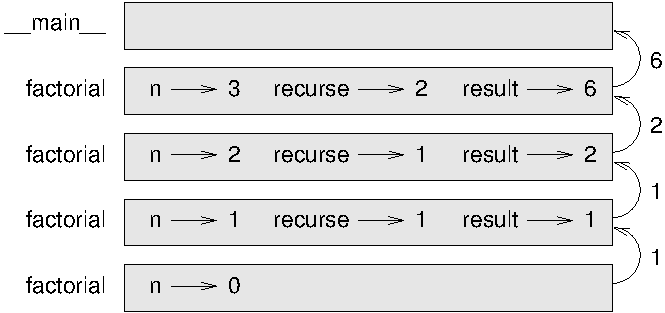
\includegraphics[scale=0.8]{../source/figs/stack3.pdf}}
\caption{堆栈图。}
\label{fig.stack3}
\end{figure}

%🍁% The return values are shown being passed back up the stack.  In each
%🍁% frame, the return value is the value of {\tt result}, which is the
%🍁% product of {\tt n} and {\tt recurse}.

图中的返回值被描绘为不断被传回到栈顶。 在每个栈帧中,返回值就是结果值,即是 \li{n} 和 \li{recurse} 的乘积。
\index{function frame}  \index{frame}

%🍁% In the last frame, the local variables {\tt recurse} and {\tt result} do not exist, because the branch that creates them does not run.

最后一帧中,局部变量 \li{recurse} 和 \li{result} 并不存在, 因为生成它们的分支并没有执行。


%🍁% \section{Leap of faith  |  信仰之跃}
\section{信仰之跃}
\index{recursion}  \index{leap of faith}

%🍁% Following the flow of execution is one way to read programs, but
%🍁% it can quickly become overwhelming.  An
%🍁% alternative is what I call the ``leap of faith''.  When you come to a
%🍁% function call, instead of following the flow of execution, you {\em
%🍁% assume} that the function works correctly and returns the right
%🍁% result.

跟随程序执行流程是阅读程序代码的一种方法,但它可能很快会变得错综复杂。
有另外一种替代方法,我称之为``信仰之跃''。
当你遇到一个函数调用时,不再去跟踪执行流程,而是 {\bf 假设} 这个函数正确运行并返回了正确的结果。

%🍁% In fact, you are already practicing this leap of faith when you use
%🍁% built-in functions.  When you call {\tt math.cos} or {\tt math.exp},
%🍁% you don't examine the bodies of those functions.  You just
%🍁% assume that they work because the people who wrote the built-in
%🍁% functions were good programmers.

事实上,当你使用内建函数时,你已经在实践这种方法了。
当你调用 \li{math.cos} 或 \li{math.exp} 时,你并没有检查那些函数的函数体。
你只是假设了它们能用,因为编写这些内建函数的人都是优秀的程序员。

%🍁% The same is true when you call one of your own functions.  For
%🍁% example, in Section~\ref{boolean}, we wrote a function called
%🍁% \verb"is_divisible" that determines whether one number is divisible by
%🍁% another.  Once we have convinced ourselves that this function is
%🍁% correct---by examining the code and testing---we can use the function
%🍁% without looking at the body again.

当你调用一个自己写的函数时也是一样。
例如,在 \ref{boolean} 节中,我们写了一个 \li{is_divisible} 函数来判断一个数能否被另一个数整除。
通过对代码的检查,一旦我们确信这个函数能够正确运行 --- 我们就能不用再查看函数体而直接使用了。
\index{testing!leap of faith}

%🍁% The same is true of recursive programs.  When you get to the recursive
%🍁% call, instead of following the flow of execution, you should assume
%🍁% that the recursive call works (returns the correct result) and then ask
%🍁% yourself, ``Assuming that I can find the factorial of $n-1$, can I
%🍁% compute the factorial of $n$?''  It is clear that you
%🍁% can, by multiplying by $n$.

递归程序也是这样。
当你遇到递归调用时, 不用顺着执行流程,你应该假设每次递归调用能够正确工作 (返回正确的结果), 然后问你自己,``假设我可以找到 $n-1$ 的阶乘,我可以找到 $n$ 的阶乘吗?''
很明显你能,只要再乘以 $n$ 即可。

%🍁% Of course, it's a bit strange to assume that the function works
%🍁% correctly when you haven't finished writing it, but that's why
%🍁% it's called a leap of faith!

当然,在你没写完函数的时就假设函数正确工作有一点儿奇怪, 但这也是为什么这被称作信仰之跃了!


%🍁% \section{One more example  |  再举一例}
\section{再举一例}
\label{one.more.example}

\index{fibonacci function}  \index{function!fibonacci}

%🍁% After {\tt factorial}, the most common example of a recursively
%🍁% defined mathematical function is {\tt fibonacci}, which has the
%🍁% following definition (see
  %🍁% \url{http://en.wikipedia.org/wiki/Fibonacci_number}):

除了阶乘以外,使用递归定义的最常见数学函数是 \li{fibonacci} (斐波那契数列),见其 \href{http://en.wikipedia.org/wiki/Fibonacci_number}{定义} :

\index{维基百科}

%
\begin{eqnarray*}
&& \mathrm{fibonacci}(0) = 0 \\
&& \mathrm{fibonacci}(1) = 1 \\
&& \mathrm{fibonacci}(n) = \mathrm{fibonacci}(n-1) + \mathrm{fibonacci}(n-2)
\end{eqnarray*}

%
%🍁% Translated into Python, it looks like this:

翻译成 Python ,看起来就像这样:

\begin{lstlisting}
def fibonacci (n):
    if n == 0:
        return 0
    elif  n == 1:
        return 1
    else:
        return fibonacci(n-1) + fibonacci(n-2)
\end{lstlisting}

%
%🍁% If you try to follow the flow of execution here, even for fairly
%🍁% small values of $n$, your head explodes.  But according to the
%🍁% leap of faith, if you assume that the two recursive calls
%🍁% work correctly, then it is clear that you get
%🍁% the right result by adding them together.

这里,如果你试图跟踪执行流程,即使是相当小的 $n$ ,也足够你头疼的。但遵循信仰之跃这种方法,如果你假设这两个递归调用都能正确运行,很明显将他们两个相加就是正确结果。

\index{flow of execution}


%🍁% \section{Checking types  |  检查类型}
\section{检查类型}
\label{guardian}

%🍁% What happens if we call {\tt factorial} and give it 1.5 as an argument?

如果我们将 1.5 作为参数调用阶乘函数 ( \li{factorial} )会怎样?

\index{type checking}  \index{error checking}
\index{factorial function}  \index{RuntimeError}

\begin{lstlisting}
>>> factorial(1.5)
RuntimeError: Maximum recursion depth exceeded
\end{lstlisting}

%
%🍁% It looks like an infinite recursion.  How can that be?  The function
%🍁% has a base case---when {\tt n == 0}.  But if {\tt n} is not an integer,
%🍁% we can {\em miss} the base case and recurse forever.

看上去像是一个无限循环。但那是如何发生的? 函数的基础情形是 \li{n == 0} 。
但是如果 \li{n} 不是一个整型数呢,我们会 {\em 错过} 基础情形,永远递归下去。
\index{infinite recursion}  \index{recursion!infinite}

%🍁% In the first recursive call, the value of {\tt n} is 0.5.
%🍁% In the next, it is -0.5.  From there, it gets smaller
%🍁% (more negative), but it will never be 0.

在第一次递归调用中,\li{n} 的值是 $0.5$ 。下一次,是 $-0.5$ 。自此它会越来越小,但永远不会是 $0$ 。

%🍁%  We have two choices.  We can try to generalize the {\tt factorial}
%🍁%  function to work with floating-point numbers, or we can make {\tt
  %🍁%  factorial} check the type of its argument.  The first option is
%🍁%  called the gamma function and it's a
%🍁%  little beyond the scope of this book.  So we'll go for the second.

我们有两个选择。我们可以试着泛化 \li{factorial} 函数,使其能处理浮点数,或者我们可以让 \li{factorial} 检查实参的类型。第一个选择被称作 \li{gamma} 函数,它有点儿超过本书的范围了。 所以我们将采用第二种方法。
\index{gamma function}
\index{gamma 函数}

%🍁% We can use the built-in function {\tt isinstance} to verify the type
%🍁% of the argument.  While we're at it, we can also make sure the
%🍁% argument is positive:

我们可以使用内建函数 \li{isinstance} 来验证实参的类型。 同时,我们也可以确保该实参是正数:
\index{isinstance function}  \index{function!isinstance}

\begin{lstlisting}
def factorial (n):
    if not isinstance(n, int):
        print('Factorial is only defined for integers.')
        return None
    elif n < 0:
        print('Factorial is not defined for negative integers.')
        return None
    elif n == 0:
        return 1
    else:
        return n * factorial(n-1)
\end{lstlisting}

%
%🍁% The first base case handles nonintegers; the
%🍁% second handles negative integers.  In both cases, the program prints
%🍁% an error message and returns {\tt None} to indicate that something
%🍁% went wrong:

第一个基础情形处理非整型数;第二个处理负整型数。
在这两个情形中,程序打印一条错误信息,并返回 \li{None} 以指明出现了错误:


\begin{lstlisting}
>>> factorial('fred')
Factorial is only defined for integers.
None
>>> factorial(-2)
Factorial is not defined for negative integers.
None
\end{lstlisting}

%
%🍁% If we get past both checks, we know that $n$ is positive or
%🍁% zero, so we can prove that the recursion terminates.

如果我们通过了这两个检查,那么我们知道 $n$ 是一个正数或 $0$ , 因此我们可以证明递归会终止。
\index{guardian pattern}  \index{pattern!guardian}

%🍁% This program demonstrates a pattern sometimes called a {\bf guardian}.
%🍁% The first two conditionals act as guardians, protecting the code that
%🍁% follows from values that might cause an error.  The guardians make it
%🍁% possible to prove the correctness of the code.

此程序演示了一个有时被称作 {\em 监护人} (guardian) 的模式。
前两个条件扮演监护人的角色,避免接下来的代码使用引发错误的值。
监护人使得验证代码的正确性成为可能。


%🍁% In Section~\ref{raise} we will see a more flexible alternative to printing
%🍁% an error message: raising an exception.

在\hyperref[raise]{反向查找} (Reverse Lookup) 一节中,我们将看到更灵活地打印错误信息的方式:抛出异常。

%🍁% \section{Debugging  |  调试}
\section{调试}
\label{factdebug}

%🍁% Breaking a large program into smaller functions creates natural
%🍁% checkpoints for debugging.  If a function is not
%🍁% working, there are three possibilities to consider:

将一个大程序分解为较小的函数为调试生成了自然的检查点。
如果一个函数不如预期的运行,有三个可能性需要考虑:

\index{debugging}

\begin{itemize}

%🍁% \item There is something wrong with the arguments the function
%🍁% is getting; a precondition is violated.

\item 该函数获得的实参有些问题,违反先决条件。

%🍁% \item There is something wrong with the function; a postcondition
%🍁% is violated.

\item 该函数有些问题,违反后置条件。

%🍁% \item There is something wrong with the return value or the
%🍁% way it is being used.

\item 返回值或者它的使用方法有问题。

\end{itemize}

%🍁% To rule out the first possibility, you can add a {\tt print} statement
%🍁% at the beginning of the function and display the values of the
%🍁% parameters (and maybe their types).  Or you can write code
%🍁% that checks the preconditions explicitly.

为了排除第一种可能,你可以在函数的开始增加一条 \li{print} 语句来打印形参的值(也可以是它们的类型)。
或者你可以写代码来显示地检查先决条件。
\index{precondition}  \index{postcondition}

%🍁% If the parameters look good, add a {\tt print} statement before each
%🍁% {\tt return} statement and display the return value.  If
%🍁% possible, check the result by hand.  Consider calling the
%🍁% function with values that make it easy to check the result
%🍁% (as in Section~\ref{incremental.development}).

如果形参看起来没问题,就在每个 \li{return} 语句之前增加一条 \li{print} 语句,来打印返回值。
如果可能,手工检查结果。
考虑用一些容易检查的值来调用该函数(类似在 \hyperref[incremental.development]{小节} 中那样)。


%🍁% If the function seems to be working, look at the function call
%🍁% to make sure the return value is being used correctly (or used
%🍁% at all!).

如果该函数看起来正常工作,则检查函数调用,确保返回值被正确的使用(或者的确被使用了!)。
\index{flow of execution}

%🍁% Adding print statements at the beginning and end of a function
%🍁% can help make the flow of execution more visible.
%🍁% For example, here is a version of {\tt factorial} with
%🍁% print statements:

在一个函数的开始和结尾处增加打印语句,可以使执行流程更明显。
例如,下面是一个带打印语句的阶乘函数:

\begin{lstlisting}
def factorial(n):
    space = ' ' * (4 * n)
    print(space, 'factorial', n)
    if n == 0:
        print(space, 'returning 1')
        return 1
    else:
        recurse = factorial(n-1)
        result = n * recurse
        print(space, 'returning', result)
        return result
\end{lstlisting}

%
%🍁% {\tt space} is a string of space characters that controls the
%🍁% indentation of the output.  Here is the result of {\tt factorial(4)} :

\li{space} 是一个空格字符的字符串,用来控制输出的缩进。 下面是 \li{factorial(4)} 的输出结果:


\begin{lstlisting}
                 factorial 4
             factorial 3
         factorial 2
     factorial 1
 factorial 0
 returning 1
     returning 1
         returning 2
             returning 6
                 returning 24
\end{lstlisting}

%
%🍁% If you are confused about the flow of execution, this kind of
%🍁% output can be helpful.  It takes some time to develop effective
%🍁% scaffolding, but a little bit of scaffolding can save a lot of debugging.

如果你对执行流程感到困惑,这种输出可能有助于理解。
开发有效的脚手架代码会花些时间,但是一点点的脚手架代码能够节省很多的调试时间。

%🍁% \section{Glossary  |  术语表}
\section{术语表}

\begin{description}

%🍁% \item[temporary variable:]  A variable used to store an intermediate value in
%🍁% a complex calculation.
\index{temporary variable}  \index{variable!temporary}
\index{临时变量}  \index{变量!临时}

\item[临时变量 (temporary variable):] 一个在复杂计算中用于存储过度值的变量。

%🍁% \item[dead code:]  Part of a program that can never run, often because
%🍁% it appears after a {\tt return} statement.
\index{dead code}
\index{死代码}

\item[死代码 (dead code):] 程序中永远无法执行的那部分代码,通常是因为其出现在一个返回语句之后。

%🍁% \item[incremental development:]  A program development plan intended to
%🍁% avoid debugging by adding and testing only
%🍁% a small amount of code at a time.
\index{incremental development}
\index{增量式开发}

\item[增量式开发 (incremental development):] 一种程序开发计划,目的是通过一次增加及测试少量代码的方式,来避免长时间的调试。

%🍁% \item[scaffolding:]  Code that is used during program development but is
%🍁% not part of the final version.
\index{scaffolding}
\index{脚手架代码}

\item[脚手架代码 (scaffolding):] 程序开发中使用的代码,但并不是最终版本的一部分。

%🍁% \item[guardian:]  A programming pattern that uses a conditional
%🍁% statement to check for and handle circumstances that
%🍁% might cause an error.
\index{guardian pattern}  \index{pattern!guardian}
\index{监护人模式}  \index{模式!监护人}

\item[监护人 (guardian):] 一种编程模式,使用条件语句来检查并处理可能引发错误的情形。

\end{description}


%🍁% \section{Exercises  |  练习}
\section{练习}

\begin{exercise}

%🍁% Draw a stack diagram for the following program.  What does the program print?

画出下面程序的堆栈图。
这个程序的最终输出是什么?
\index{stack diagram}  \index{堆栈图}

\begin{em}
\begin{lstlisting}
def b(z):
    prod = a(z, z)
    print(z, prod)
    return prod

def a(x, y):
    x = x + 1
    return x * y

def c(x, y, z):
    total = x + y + z
    square = b(total)**2
    return square

x = 1
y = x + 1
print(c(x, y+3, x+y))
\end{lstlisting}
\end{em}

\end{exercise}


\begin{exercise}
\label{ackermann}

%🍁% The Ackermann function, $A(m, n)$, is defined:

{\em Ackermann} 函数 $A(m, n)$ 的定义如下:

\begin{eqnarray*}
A(m, n) = \begin{cases}
              n+1 & \mbox{if } m = 0 \\
        A(m-1, 1) & \mbox{if } m > 0 \mbox{ and } n = 0 \\
A(m-1, A(m, n-1)) & \mbox{if } m > 0 \mbox{ and } n > 0.
\end{cases}
\end{eqnarray*}

%
%🍁% See \url{http://en.wikipedia.org/wiki/Ackermann_function}.
%🍁% Write a function named {\tt ack} that evaluates the Ackermann function.
%🍁% Use your function to evaluate {\tt ack(3, 4)}, which should be 125.
%🍁% What happens for larger values of {\tt m} and {\tt n}?
%🍁% Solution: \url{http://thinkpython2.com/code/ackermann.py}.

查看 \href{http://en.wikipedia.org/wiki/Ackermann_function}{维基百科的定义},
编写一个叫作 {\em \li{ack}} 的函数来计算 {\em Ackermann} 函数。
使用你的函数计算 {\em \li{ack(3,4)}},其结果应该为 $125$ 。
如果 {\em \li{m}} 和 {\em \li{n}} 的值较大时,会发生什么?
\href{http://thinkpython2.com/code/ackermann.py}{参考答案}

\index{Ackermann function}  \index{function!ack}
\index{阿克曼函数}  \index{函数!阿克曼}
\index{维基百科}
\end{exercise}


\begin{exercise}
\label{palindrome}

%🍁% A palindrome is a word that is spelled the same backward and
%🍁% forward, like ``noon'' and ``redivider''.  Recursively, a word
%🍁% is a palindrome if the first and last letters are the same
%🍁% and the middle is a palindrome.

回文词 {\em (palindrome)} 指的是正着拼反着拼都一样的单词,如 {\em ``noon''} 和 {\em ``redivider''}。
按照递归定义的话, 如果某个词的首字母和尾字母相同, 而且中间部分也是一个回文词, 那它就是一个回文词。
\index{palindrome}

%🍁% The following are functions that take a string argument and
%🍁% return the first, last, and middle letters:

下面的函数接受一个字符串实参,并返回第一个、最后一个和中间的字母:

\begin{em}
\begin{lstlisting}
def first(word):
    return word[0]

def last(word):
    return word[-1]

def middle(word):
    return word[1:-1]
\end{lstlisting}
\end{em}

%
%🍁% We'll see how they work in Chapter~\ref{strings}.

在 \hyperref[strings]{第八章} 中我们将介绍它们是如何工作的。

%🍁% \begin{enumerate}
%🍁%
%🍁% \item Type these functions into a file named {\tt palindrome.py}
%🍁% and test them out.  What happens if you call {\tt middle} with
%🍁% a string with two letters?  One letter?  What about the empty
%🍁% string, which is written \verb"''" and contains no letters?
%🍁%
%🍁% \item Write a function called \verb"is_palindrome" that takes
%🍁% a string argument and returns {\tt True} if it is a palindrome
%🍁% and {\tt False} otherwise.  Remember that you can use the
%🍁% built-in function {\tt len} to check the length of a string.
%🍁%
%🍁% \end{enumerate}

\begin{enumerate}

\item 将它们录入到文件 {\em \li{palindrome.py}} 中并测试。当你用一个两个字母的字符串调用 {\em \li{middle}} 时会发生什么?一个字母的呢?空字符串呢?空字符串这样 {\em \li{"''"}} 表示,中间不含任何字母。

\item 编写一个叫 {\em \li{is_palindrome}} 的函数, 接受一个字符串作为实参。 如果是回文词, 就返回 {\em \li{True}} ,反之则返回 {\em \li{False}} 。记住, 你可以使用内建函数 {\em \li{len}} 来检查字符串的长度。

\end{enumerate}

%🍁% Solution: \url{http://thinkpython2.com/code/palindrome_soln.py}.

\href{http://thinkpython2.com/code/palindrome_soln.py}{参考答案}

\end{exercise}

\begin{exercise}

%🍁% A number, $a$, is a power of $b$ if it is divisible by $b$
%🍁% and $a/b$ is a power of $b$.  Write a function called
%🍁% \verb"is_power" that takes parameters {\tt a} and {\tt b}
%🍁% and returns {\tt True} if {\tt a} is a power of {\tt b}.
%🍁% Note: you will have to think about the base case.

当数字 $a$ 能被  $b$ 整除,并且 $a/b$ 是 $b$ 的幂时, 它就是 $b$ 的幂。
编写一个叫 {\em \li{is_power}} 的函数,接受两个参数 {\em \li{a}} 和 {\em \li{b}}, 并且当 {\em \li{a}} 是 {\em \li{b}} 的幂时返回 {\em \li{True}}。
注意:你必须要想好基础情形。

\end{exercise}

\begin{exercise}
\index{greatest common divisor (GCD)}  \index{GCD (greatest common divisor)}

%🍁% The greatest common divisor (GCD) of $a$ and $b$ is the largest number
%🍁% that divides both of them with no remainder.

$a$ 和 $b$ 的最大公约数 {\em (reatest common divisor, GCD)}是能被二者整除的最大数。

%🍁% One way to find the GCD of two numbers is based on the observation
%🍁% that if $r$ is the remainder when $a$ is divided by $b$, then $gcd(a,
%🍁% b) = gcd(b, r)$.  As a base case, we can use $gcd(a, 0) = a$.

求两个数的最大公约数的一种方法,是基于这样一个原理:如果 $r$ 是 $a$ 被 $b$ 除后的余数,那么  $gcd(a,b) = gcd(b, r)$ 。我们可以把 $gcd(a, 0) = a$ 当做基础情形。

%🍁% Write a function called
%🍁% \verb"gcd" that takes parameters {\tt a} and {\tt b}
%🍁% and returns their greatest common divisor.

编写一个叫 {\em \li{gcd}} 的函数,接受两个参数 {\em \li{a}} 和 {\em \li{b}},并返回二者的最大公约数。

%🍁% Credit: This exercise is based on an example from Abelson and
%🍁% Sussman's {\em Structure and Interpretation of Computer Programs}.

致谢:这道习题基于 {\em Abelson} 和 {\em Sussman} 编写的 《Structure and Interpretation of Computer Programs》 中的例子。

\end{exercise}




%🍁% \chapter{Iteration  |  迭代}
\chapter{迭代}

%🍁% This chapter is about iteration, which is the ability to run
%🍁% a block of statements repeatedly.  We saw a kind of iteration,
%🍁% using recursion, in Section~\ref{recursion}.
%🍁% We saw another kind, using a {\tt for} loop,
%🍁% in Section~\ref{repetition}.  In this chapter we'll see yet another
%🍁% kind, using a {\tt while} statement.
%🍁% But first I want to say a little more about variable assignment.

本章介绍迭代,即重复运行某个代码块的能力。我们已经在~\ref{recursion} 节接触了一种利用递归进行迭代的方式;在~\ref{repetition} 节中,接触了另一种利用 \li{for} 循环进行迭代的方式。 在本章中,我们将讨论另外一种利用 \li{while} 语句实现迭代的方式。
不过,首先我想再多谈谈有关变量赋值的问题。

%🍁%  \section{Reassignment  |  重新赋值}
\section{重新赋值}
\index{assignment}  \index{statement!assignment}  \index{reassignment}
\index{赋值}  \index{语句!赋值}  \index{重新赋值}

%🍁% As you may have discovered, it is legal to make more than one
%🍁% assignment to the same variable.  A new assignment makes an existing
%🍁% variable refer to a new value (and stop referring to the old value).

可能你已发现对同一变量进行多次赋值是合法的。 新的赋值会使得已有的变量指向
新的值(同时不再指向旧的值)。

\begin{lstlisting}
>>> x = 5
>>> x
5
>>> x = 7
>>> x
7
\end{lstlisting}

%
%🍁% The first time we display
%🍁% {\tt x}, its value is 5; the second time, its
%🍁% value is 7.

第一次打印 \li{x} 时, 它的值为 \li{5};第二次打印时,它的值是 \li{7}。

%🍁% Figure~\ref{fig.assign2} shows what {\bf reassignment} looks
%🍁% like in a state diagram.
%🍁% \index{state diagram} \index{diagram!state}

图~\ref{fig.assign2} 展示了 {\em 重新赋值} 在状态图中看起来是什么样子。
\index{state diagram} \index{diagram!state}

%🍁% At this point I want to address a common source of confusion.
%🍁% Because Python uses the equal sign ({\tt =}) for assignment, it is
%🍁% tempting to interpret a statement like {\tt a = b} as a mathematical
%🍁% proposition of equality; that is, the claim that {\tt a} and
%🍁% {\tt b} are equal.  But this interpretation is wrong.
%🍁% \index{equality and assignment}

这里我想探讨一个常见的疑惑点。由于 Python 用等号 (\li{=}) 来赋值,所以很容易将 \li{a = b} 这样的语句理解为数学上的相等命题;即 \li{a} 和 \li{b} 相等。但是这种理解是错误的。

%🍁% First, equality is a symmetric relationship and assignment is not.  For
%🍁% example, in mathematics, if $a=7$ then $7=a$.  But in Python, the
%🍁% statement {\tt a = 7} is legal and {\tt 7 = a} is not.

首先,相等是一种对称关系,赋值不是。例如,在数学上,如果 $a = 7$,
则 $7 = a$。 但是在 Python 中,语句 \li{a = 7} 是合法的, \li{7 = a} 则不合法。

%🍁% Also, in mathematics, a proposition of equality is either true or
%🍁% false for all time.  If $a=b$ now, then $a$ will always equal $b$.
%🍁% In Python, an assignment statement can make two variables equal, but
%🍁% they don't have to stay that way:

此外,数学中,相等命题不是对的就是错的。 如果 $a = b$,那么 $a$
则是永远与 $b$ 相等。在 Python 中,赋值语句可以使得两个变量相等,
但是这两个变量不一定必须保持这个状态:


\begin{lstlisting}
>>> a = 5
>>> b = a    # a and b are now equal
>>> a = 3    # a and b are no longer equal
>>> b
5
\end{lstlisting}

%
%🍁% The third line changes the value of {\tt a} but does not change the
%🍁% value of {\tt b}, so they are no longer equal.

第三行改变了 \li{a} 的值,但是没有改变 \li{b} 的值,所以它们不再相等了。

%🍁% Reassigning variables is often useful, but you should use it
%🍁% with caution.  If the values of variables change frequently, it can
%🍁% make the code difficult to read and debug.

给变量重新赋值非常有用,但是需要小心使用。 对变量频繁重新赋值会使代码难于阅读,
不易调试。

\begin{figure}
\centerline
{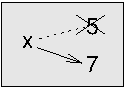
\includegraphics[scale=0.8]{../source/figs/assign2.pdf}}
% \caption {State diagram.}
\caption {重新赋值的状态图。}
\label{fig.assign2}
\end{figure}


%🍁% \section{Updating variables  |  更新变量}
\section{更新变量}
\label{update}

\index{update}  \index{variable!updating}
\index{更新}  \index{变量!更新}

%🍁% A common kind of reassignment is an {\bf update},
%🍁% where the new value of the variable depends on the old.

重新赋值的一个常见方式是 {\em 更新} (update) , 更新操作中变量的新值会取决于旧值。


\begin{lstlisting}
>>> x = x + 1
\end{lstlisting}

%
%🍁% This means ``get the current value of {\tt x}, add one, and then
%🍁% update {\tt x} with the new value.''

这个语句的意思是,``获得 \li{x} 的当前值并与 \li{1} 做加法求和,然后将 \li{x} 的值更新为所求的和。''

%🍁% If you try to update a variable that doesn't exist, you get an
%🍁% error, because Python evaluates the right side before it assigns
%🍁% a value to {\tt x}:

如果试图去更新一个不存在的变量,则会返回一个错误。 这是因为 Python 是先求
式子右边的值,然后再把所求的值赋给 \li{x}:

\begin{lstlisting}
>>> x = x + 1
NameError: name 'x' is not defined
\end{lstlisting}

%
%🍁% Before you can update a variable, you have to {\bf initialize}
%🍁% it, usually with a simple assignment:
\index{initialization (before update)}

在更新变量之前,你得先 {\em 初始化} (initialize) 它,通常是通过一个简单的赋值实现:
\index{initialization (before update)}

\begin{lstlisting}
>>> x = 0
>>> x = x + 1
\end{lstlisting}

%
%🍁% Updating a variable by adding 1 is called an {\bf increment};
%🍁% subtracting 1 is called a {\bf decrement}.
\index{increment}  \index{decrement}

通过加 \li{1} 来更新变量叫做 {\em 递增} (increment); 减 \li{1} 叫做 {\em 递减} (decrement)。
\index{increment}  \index{decrement}

%🍁% \section{The {\tt while} statement  |  {\tt while} 语句}
\section{{\tt while} 语句}
\index{statement!while}  \index{while loop}
\index{loop!while}  \index{iteration}

%🍁% Computers are often used to automate repetitive tasks.  Repeating
%🍁% identical or similar tasks without making errors is something that
%🍁% computers do well and people do poorly.  In a computer program,
%🍁% repetition is also called {\bf iteration}.

计算机经常被用来自动处理重复性的任务。 计算机很擅长无纰漏地重复相同或者相似的任务, 而人类在这方面做的不好。 在计算机程序中, 重复也被称为 {\em 迭代} (iteration)。

%🍁% We have already seen two functions, {\tt countdown} and
%🍁% \verb"print_n", that iterate using recursion.  Because iteration is so
%🍁% common, Python provides language features to make it easier.
%🍁% One is the {\tt for} statement we saw in Section~\ref{repetition}.
%🍁% We'll get back to that later.

我们已经见过两个利用递归来迭代的函数: \li{countdown} 和 \li{print_n} 。 由于迭代的使用非常普遍, 所以 Python 提供了使其更容易实现的语言特性。 其中之一就是我们在~\:ref{repetition} 一节看到的 \li{for} 语句。 后面我们还会继续介绍。

% add hyperref of 后面 here

%🍁% Another is the {\tt while} statement.  Here is a version of {\tt
%🍁% countdown} that uses a {\tt while} statement:

另外一个用于迭代的语句是 \li{while} 。 下面是使用 \li{while} 语句实现的 \li{countdown}:

\begin{lstlisting}
def countdown(n):
    while n > 0:
        print(n)
        n = n - 1
    print('Blastoff!')
\end{lstlisting}

%
%🍁% You can almost read the {\tt while} statement as if it were English.
%🍁% It means, ``While {\tt n} is greater than 0,
%🍁% display the value of {\tt n} and then decrement
%🍁% {\tt n}.  When you get to 0, display the word {\tt Blastoff!}''
\index{flow of execution}

你可以像读英语句子一样来读 \li{while} 语句。 它的意思是:``只要 \li{n} 的值大于 \li{0}, 则打印出 \li{n} 的值,然后让 \li{n} 减 \li{1}。 当 \li{n} 递减至 \li{0} 时,打印单词 \li{Blastoff}!''。

%🍁% More formally, here is the flow of execution for a {\tt while} statement:

更正式地来说,\li{while} 语句的执行流程如下:

%🍁% \begin{enumerate}
%🍁%
%🍁% \item Determine whether the condition is true or false.
%🍁%
%🍁% \item If false, exit the {\tt while} statement
%🍁% and continue execution at the next statement.
%🍁%
%🍁% \item If the condition is true, run the
%🍁% body and then go back to step 1.
%🍁%
%🍁% \end{enumerate}

\begin{enumerate}

\item 首先判断条件为 {\bf 真} 还是为 {\bf 假}。

\item 如果为假,退出 \li{while} 语句,然后执行接下来的语句;

\item 如果条件为真,则运行 \li{while} 语句 {\em 循环主体},运行完再返回第一步;

\end{enumerate}

%🍁% This type of flow is called a loop because the third step
%🍁% loops back around to the top.
\index{condition}  \index{loop}  \index{body}

这种形式的流程叫做 {\em 循环} (loop), 因为第三步后又循环回到了第一步。
\index{condition}  \index{loop}  \index{body}

%🍁% The body of the loop should change the value of one or more variables
%🍁% so that the condition becomes false eventually and the loop
%🍁% terminates.  Otherwise the loop will repeat forever, which is called
%🍁% an {\bf infinite loop}.  An endless source of amusement for computer
%🍁% scientists is the observation that the directions on shampoo,
%🍁% ``Lather, rinse, repeat'', are an infinite loop.
\index{infinite loop}  \index{loop!infinite}

循环主体应该改变一个或多个变量的值,这样的话才能让条件判断最终变为假,
从而终止循环。 否则,循环将会永远重复下去,这被称为 {\em 无限循环} (infinite loop)。 在计算机科学家看来,洗发水的使用说明 —— ``抹洗发水,
清洗掉,重复'' 便是个无限循环,这总是会让他们觉得好笑。
\index{infinite loop}  \index{loop!infinite}

%🍁% In the case of {\tt countdown}, we can prove that the loop
%🍁% terminates: if {\tt n} is zero or negative, the loop never runs.
%🍁% Otherwise, {\tt n} gets smaller each time through the
%🍁% loop, so eventually we have to get to 0.

对于 \li{countdown} 来说,我们可以证明循环是一定会终止的:当 n 是 0 或者负数,该循环就不会执行;不然 n 通过每次循环之后慢慢减小,最终也是会变成 0 的。

%🍁% For some other loops, it is not so easy to tell.  For example:

有些其他循环,可能就没那么好理解了。例如:

\begin{lstlisting}
def sequence(n):
    while n != 1:
        print(n)
        if n % 2 == 0:        # n is even
            n = n / 2
        else:                 # n is odd
            n = n*3 + 1
\end{lstlisting}

%
%🍁% The condition for this loop is {\tt n != 1}, so the loop will continue
%🍁% until {\tt n} is {\tt 1}, which makes the condition false.

循环的条件是 \li{n != 1},所以循环会一直执行到 \li{n} 等于 \li{1},条件判断为假时循环才终止。

%🍁% Each time through the loop, the program outputs the value of {\tt n}
%🍁% and then checks whether it is even or odd.  If it is even, {\tt n} is
%🍁% divided by 2.  If it is odd, the value of {\tt n} is replaced with
%🍁% {\tt n*3 + 1}. For example, if the argument passed to {\tt sequence}
%🍁% is 3, the resulting values of {\tt n} are 3, 10, 5, 16, 8, 4, 2, 1.

每次循环,该程序打印出 \li{n} 的值,然后检查它是偶数还是奇数。如果它是偶数,
那么 \li{n} 可以被2整除;如果是奇数,则它的值被替换为 \li {n*3 + 1}。 例如,如果传递给 \li{sequence} 的实参为3, 那么打印出的结果将会是:\li{3}、 \li{10}、 \li{5}、 \li{16}、 \li{8}、 \li{4}、 \li{2}、 \li{1}。

%🍁% Since {\tt n} sometimes increases and sometimes decreases, there is no
%🍁% obvious proof that {\tt n} will ever reach 1, or that the program
%🍁% terminates.  For some particular values of {\tt n}, we can prove
%🍁% termination.  For example, if the starting value is a power of two,
%🍁% {\tt n} will be even every time through the loop
%🍁% until it reaches 1. The previous example ends with such a sequence,
%🍁% starting with 16.
%🍁% \index{Collatz conjecture}

由于 \li{n} 的值时增时减,所以不能轻易保证 \li{n} 会最终变成 \li{1}, 或者说这个程序能够终止。 对于某些特殊的 \li{n} 的值,可以很好地证明它是可以终止的。 例如, 当 \li{n} 的初始值是 \li{2} 的倍数时,则每次循环后 \li{n} 一直为偶数, 直到最终变为 \li{1}。 上一个示例中,程序就打印了类似的序列, 从 \li{16} 开始全部为偶数。
\index{Collatz conjecture}

%🍁% The hard question is whether we can prove that this program terminates
%🍁% for {\em all} positive values of {\tt n}.  So far, no one has
%🍁% been able to prove it {\em or} disprove it!  (See
%🍁%   \url{http://en.wikipedia.org/wiki/Collatz_conjecture}.)

难点在于是否能证明程序对于 {\bf 所有} 的正整数 \li{n} 都会终止。 目前为止,
还没有人证明 {\bf 或者} 证伪该命题。(见:\url{http://en.wikipedia.org/wiki/Collatz_conjecture} 。)

%🍁% As an exercise, rewrite the function \verb"print_n" from
%🍁% Section~\ref{recursion} using iteration instead of recursion.

我们做个练习,利用迭代而非递归,重写之前~\ref{recursion} 节中的 \li{print_n} 函数。

%🍁% \section{{\tt break} }
\section{{\tt break} }
\index{break statement}  \index{statement!break}

%🍁% Sometimes you don't know it's time to end a loop until you get half
%🍁% way through the body.  In that case you can use the {\tt break}
%🍁% statement to jump out of the loop.

有些时候循环执行到一半你才知道循环该结束了。这种情况下,你可以使用 \li{break} 语句来跳出循环。

%🍁% For example, suppose you want to take input from the user until they
%🍁% type {\tt done}.  You could write:

例如,假设你想从用户那里获取输入,直到用户键入 \li{'done'}。 你可以这么写:

\begin{lstlisting}
while True:
    line = input('> ')
    if line == 'done':
        break
    print(line)

print('Done!')
\end{lstlisting}

%
%🍁% The loop condition is {\tt True}, which is always true, so the
%🍁% loop runs until it hits the break statement.

循环条件是 \li{True},其总是为真,所以该循环会一直执行直到碰到 \li{break}。

%🍁% Each time through, it prompts the user with an angle bracket.
%🍁% If the user types {\tt done}, the {\tt break} statement exits
%🍁% the loop.  Otherwise the program echoes whatever the user types
%🍁% and goes back to the top of the loop.  Here's a sample run:

每次循环时,程序都会给出一个尖括号 (\li{>}) 提示。 如果用户输入 \li{'done'},执行 \li{break} 语句跳出循环。 否则, 程序就会一直打印出用户所输入的内容并且跳到循环开始, 0以下是一个运行示例:


\begin{lstlisting}
> not done
not done
> done
Done!
\end{lstlisting}

%
%🍁% This way of writing {\tt while} loops is common because you
%🍁% can check the condition anywhere in the loop (not just at the
%🍁% top) and you can express the stop condition affirmatively
%🍁% (``stop when this happens'') rather than negatively (``keep going
%🍁% until that happens'').

\li{while} 循环的这种写法很常见, 因为你可以在循环的任何地方判断条件
(而不只是在循环开始), 而且你可以积极地表达终止条件(``当出现这个情况是终止''), 而不是消极地表示 (``继续运行直到出现这个情况'')。


%🍁% \section{Square roots  |  平方根}
\section{平方根}
\label{squareroot}
\index{square root}

%🍁% Loops are often used in programs that compute
%🍁% numerical results by starting with an approximate answer and
%🍁% iteratively improving it.
\index{Newton's method}

循环常用于计算数值的程序中, 这类程序一般从一个大概的值开始, 然后迭代式地进行改进。 \index{Newton's method}

%🍁% For example, one way of computing square roots is Newton's method.
%🍁% Suppose that you want to know the square root of $a$.  If you start
%🍁% with almost any estimate, $x$, you can compute a better
%🍁% estimate with the following formula:

例如,牛顿法 (Newton's method) 是计算平方根的一种方法。 假设你想求 $a$ 的平方根。 如果你从任意一个估算值 $x$ 开始, 则可以利用下面的公式计算出更为较为精确的估算值:

\[ y = \frac{x + a/x}{2} \]

%
%🍁% For example, if $a$ is 4 and $x$ is 3:

例如,假定 $a$ 是 4,$x$ 是 3:

\begin{lstlisting}
>>> a = 4
>>> x = 3
>>> y = (x + a/x) / 2
>>> y
2.16666666667
\end{lstlisting}

%
%🍁% The result is closer to the correct answer ($\sqrt{4} = 2$).  If we
%🍁% repeat the process with the new estimate, it gets even closer:

可以看到, 结果与真实值 ( $\sqrt{4} = 2$ ) 已经很接近了, 如果我们用这个值
再重新运算一遍, 它将得到更为接近的值。


\begin{lstlisting}
>>> x = y
>>> y = (x + a/x) / 2
>>> y
2.00641025641
\end{lstlisting}

%
%🍁% After a few more updates, the estimate is almost exact:
%🍁% \index{update}

再通过多几次的运算,这个估算可以说已经是很精确了。
\index{update}

\begin{lstlisting}
>>> x = y
>>> y = (x + a/x) / 2
>>> y
2.00001024003
>>> x = y
>>> y = (x + a/x) / 2
>>> y
2.00000000003
\end{lstlisting}

%
%🍁% In general we don't know ahead of time how many steps it takes
%🍁% to get to the right answer, but we know when we get there
%🍁% because the estimate
%🍁% stops changing:

一般来说, 我们事先不知道要多少步才能得到正确答案, 但是我们知道当估算值不再变动时, 我们就获得了正确的答案。

\begin{lstlisting}
>>> x = y
>>> y = (x + a/x) / 2
>>> y
2.0
>>> x = y
>>> y = (x + a/x) / 2
>>> y
2.0
\end{lstlisting}

%
%🍁% When {\tt y == x}, we can stop.  Here is a loop that starts
%🍁% with an initial estimate, {\tt x}, and improves it until it
%🍁% stops changing:

当 \li{y == x} 时,我们可以停止计算了。下面这个循环就是利用一个初始估值 \li{x},
循序渐进地计算,直到估值不再变化。

\begin{lstlisting}
while True:
    print(x)
    y = (x + a/x) / 2
    if y == x:
        break
    x = y
\end{lstlisting}

%
%🍁% For most values of {\tt a} this works fine, but in general it is
%🍁% dangerous to test {\tt float} equality.
%🍁% Floating-point values are only approximately right:
%🍁% most rational numbers, like $1/3$, and irrational numbers, like
%🍁% $\sqrt{2}$, can't be represented exactly with a {\tt float}.
%🍁% \index{floating-point}  \index{epsilon}

对于大部分 \li{a} 的值,这个程序运行正常,不过一般来说,检查两个浮点数是否相等比较危险。浮点数只能大约表示:大多数有理数,如 $1/3$,以及无理数,
如 : $\sqrt{2}$,是不能用浮点数 ( \li{float} ) 来精确表示的。
\index{floating-point}  \index{epsilon}

%🍁% Rather than checking whether {\tt x} and {\tt y} are exactly equal, it
%🍁% is safer to use the built-in function {\tt abs} to compute the
%🍁% absolute value, or magnitude, of the difference between them:

与其检查 \li{x} 和 \li{y} 的值是否完全相等,使用内置函数 \li{abs} 来计算二者之差的绝对值或数量级更为安全:

\begin{lstlisting}
    if abs(y-x) < epsilon:
        break
\end{lstlisting}

%
%🍁% Where \verb"epsilon" has a value like {\tt 0.0000001} that
%🍁% determines how close is close enough.

这里,变量 \li{epsilon} 是一个决定其精确度的值,如 \li{0.0000001}。

%🍁% \section{Algorithms  |  算法}
\section{算法}
\index{algorithm}  \index{算法}

%🍁% Newton's method is an example of an {\bf algorithm}: it is a
%🍁% mechanical process for solving a category of problems (in this
%🍁% case, computing square roots).

牛顿法就是一个 {\em 算法} (Algorithm) 示例: 它是解决一类问题的计算机制
(本例中是计算平方根)。

%🍁% To understand what an algorithm is, it might help to start with
%🍁% something that is not an algorithm.  When you learned to multiply
%🍁% single-digit numbers, you probably memorized the multiplication table.
%🍁% In effect, you memorized 100 specific solutions.  That kind of
%🍁% knowledge is not algorithmic.

为了理解算法是什么,先了解什么不是算法或许有点帮助。 你在学习一位数乘法时,
可能背出了乘法表。 实际上,你只是记住了 100 个确切的答案。 这种知识并{\bf 不是}算法性的。

%🍁% But if you were ``lazy'', you might have learned a few
%🍁% tricks.  For example, to find the product of $n$ and 9, you can
%🍁% write $n-1$ as the first digit and $10-n$ as the second
%🍁% digit.  This trick is a general solution for multiplying any
%🍁% single-digit number by 9.  That's an algorithm!
%🍁% \index{addition with carrying}  \index{carrying, addition with}
%🍁% \index{subtraction!with borrowing}  \index{borrowing, subtraction with}

不过, 如果你想找 ``懒人方法'', 你可能就会找到一些诀窍。 比如为了计算 $n$
和 $9$ 的乘积,你可以把 $n-1$ 作为乘积的第一位数,再把 $10-n$
作为第二位数,从而得到它们的乘积。 这个诀窍是将任意个位数
与 $9$ 相乘的普遍解法。 这就{\bf 是}一种算法。
\index{addition with carrying}  \index{carrying, addition with}
\index{subtraction!with borrowing}  \index{borrowing, subtraction with}

%🍁% Similarly, the techniques you learned for addition with carrying,
%🍁% subtraction with borrowing, and long division are all algorithms.  One
%🍁% of the characteristics of algorithms is that they do not require any
%🍁% intelligence to carry out.  They are mechanical processes where
%🍁% each step follows from the last according to a simple set of rules.

类似地,你所学过的进位加法、借位减法、以及长除法都是算法。算法的特点之一
就是不需要过多的脑力计算。算法是一个机械的过程,每一步都是依
据一组简单的规则跟着上一步来执行的。

%🍁% Executing algorithms is boring, but designing them is interesting,
%🍁% intellectually challenging, and a central part of computer science.

执行算法的过程是很乏味的,但是设计算法就比较有趣了,不但是智
力上的挑战,更是计算机科学的核心。

%🍁% Some of the things that people do naturally, without difficulty or
%🍁% conscious thought, are the hardest to express algorithmically.
%🍁% Understanding natural language is a good example.  We all do it, but
%🍁% so far no one has been able to explain {\em how} we do it, at least
%🍁% not in the form of an algorithm.

一些人们自然而然无需下意识做到的事情,往往是难于用算法表达。 理解自然语言就是这样的。 我们每个人都听得懂自然语言, 但是目前还没有人能够解释我们是 {\bf 怎么} 做到的, 至少无法以算法的形式解释。

%🍁% \section{Debugging  |  调试}
\section{调试}
\label{bisectbug}

%🍁% As you start writing bigger programs, you might find yourself
%🍁% spending more time debugging.  More code means more chances to
%🍁% make an error and more places for bugs to hide.
%🍁% \index{debugging!by bisection}  \index{bisection, debugging by}

当你开始写更为复杂的程序时,你会发现大部分时间都花费在调试上。 更多的
代码意味着更高的出错概率,并且会有更多隐藏 bug 的地方。
\index{debugging!by bisection}  \index{bisection, debugging by}

%🍁% One way to cut your debugging time is ``debugging by bisection''.
%🍁% For example, if there are 100 lines in your program and you
%🍁% check them one at a time, it would take 100 steps.

减少调试时间的一个方法就是“对分调试”。例如,如果程序有100行,你一次检查一行,就需要100步。

%🍁% Instead, try to break the problem in half.  Look at the middle
%🍁% of the program, or near it, for an intermediate value you
%🍁% can check.  Add a {\tt print} statement (or something else
%🍁% that has a verifiable effect) and run the program.

相反, 试着将问题拆为两半。 在代码中间部分或者附近的地方, 寻找一个可以检查的中间值。 加上一行 \li{print} 语句 (或是其他具有可验证效果的代码), 然后运行程序。

%🍁% If the mid-point check is incorrect, there must be a problem in the
%🍁% first half of the program.  If it is correct, the problem is
%🍁% in the second half.

如果中间点检查出错了, 那么就说明程序的前半部分存在问题。 如果没问题, 则说明是后半部分出错了。

%🍁% Every time you perform a check like this, you halve the number of
%🍁% lines you have to search.  After six steps (which is fewer than 100),
%🍁% you would be down to one or two lines of code, at least in theory.

每次你都这样检查, 就可以将需要搜索的代码行数减少一半。 经过6步之后(这比100小多了), 你将会找到那或者两行出错的代码, 至少理论上是这样。

%🍁% In practice it is not always clear what
%🍁% the ``middle of the program'' is and not always possible to
%🍁% check it.  It doesn't make sense to count lines and find the
%🍁% exact midpoint.  Instead, think about places
%🍁% in the program where there might be errors and places where it
%🍁% is easy to put a check.  Then choose a spot where you
%🍁% think the chances are about the same that the bug is before
%🍁% or after the check.

在实践中, 可能并不能很好的确定程序的 ``中间部分'' 是什么, 也有可能并不是那么好检查。
计算行数并且取其中间行是没有意义的。 相反, 多考虑下程序中哪些地方比较容易出问题, 或者哪些地方比较容易进行检查。 然后选定一个检查点, 在这个断点前后出现bug的概念差不多。

%🍁% \section{Glossary  |  术语表}
\section{术语表}

\begin{description}

%🍁% \item[reassignment:] Assigning a new value to a variable that
%🍁% already exists.
%🍁% \index{reassignment}

\item[重新赋值(reassignment):] 给已经存在的变量赋一个新的值。
\index{reassignment}

%🍁% \item[update:] An assignment where the new value of the variable
%🍁% depends on the old.
%🍁% \index{update}

\item[更新(update):] 变量的新值取决于旧值的一种赋值方法。
\index{update}

%🍁% \item[initialization:] An assignment that gives an initial value to
%🍁% a variable that will be updated.
%🍁% \index{initialization!variable}

\item[初始化(initialize):] 给后面将要更新的变量一个初始值的一种赋值方法。
\index{initialization!variable}

%🍁% \item[increment:] An update that increases the value of a variable
%🍁% (often by one).
%🍁% \index{increment}

\item[递增(increment):] 通过增加变量的值的方式更新变量(通常是加 1)。
\index{increment}

%🍁% \item[decrement:] An update that decreases the value of a variable.
%🍁% \index{decrement}

\item[递减(decrement):] 通过减少变量的值的方式来更新变量。
\index{decrement}

%🍁% \item[iteration:] Repeated execution of a set of statements using
%🍁% either a recursive function call or a loop.
%🍁% \index{iteration}

\item[迭代(iteration):] 利用递归或者循环的方式来重复执行代一组语句的过程。
\index{iteration}

%🍁% \item[infinite loop:] A loop in which the terminating condition is
%🍁% never satisfied.
%🍁% \index{infinite loop}

\item[无限循环(infinite loop):] 无法满足终止条件的循环。
\index{infinite loop}

%🍁% \item[algorithm:]  A general process for solving a category of
%🍁% problems.
%🍁% \index{algorithm}

\item[算法(algorithm):] 解决一类问题的通用过程。
\index{algorithm}

\end{description}

%🍁% \section{Exercises  |  练习}
\section{练习}

\begin{exercise}
\index{algorithm!square root}

%🍁% Copy the loop from Section~\ref{squareroot}
%🍁% and encapsulate it in a function called
%🍁% \verb"mysqrt" that takes {\tt a} as a parameter, chooses a
%🍁% reasonable value of {\tt x}, and returns an estimate of the square
%🍁% root of {\tt a}.  \index{encapsulation}

复制 \ref{squareroot} 小节中的循环, 将其封装进一个叫 {\em \li{mysqrt}} 的函数中。 这个函数接受 {\em \li{a}} 作为形参,选择一个合适的 {\em \li{x}} 值,并返回 {\em \li{a}} 的平方根估算值。

%🍁% To test it, write a function named \verb"test_square_root"
%🍁% that prints a table like this:

为测试上面的函数,编写一个名为 {\em \li{test_squre_root}} 的函数,打印出如下表格:

\begin{em}
\begin{lstlisting}
a   mysqrt(a)     math.sqrt(a)  diff
-   ---------     ------------  ----
1.0 1.0           1.0           0.0
2.0 1.41421356237 1.41421356237 2.22044604925e-16
3.0 1.73205080757 1.73205080757 0.0
4.0 2.0           2.0           0.0
5.0 2.2360679775  2.2360679775  0.0
6.0 2.44948974278 2.44948974278 0.0
7.0 2.64575131106 2.64575131106 0.0
8.0 2.82842712475 2.82842712475 4.4408920985e-16
9.0 3.0           3.0           0.0
\end{lstlisting}
\end{em}

%
%🍁% The first column is a number, $a$; the second column is the square
%🍁% root of $a$ computed with \verb"mysqrt"; the third column is the
%🍁% square root computed by {\tt math.sqrt}; the fourth column is the
%🍁% absolute value of the difference between the two estimates.

其中第一列是 $a$ 的值;第二列是通过 {\em \li{mysqrt}} 计算得到的 $a$ 的平方根; 第三列是用 {\em \li{math.sqrt}} 计算得到的平方根; 第四列则是这两个平方根之差的绝对值。

\end{exercise}


\begin{exercise}
\index{eval function}  \index{function!eval}

%🍁% The built-in function {\tt eval} takes a string and evaluates
%🍁% it using the Python interpreter.  For example:

内置函数 {\em \li{eval}} 接受一个字符串,并使用 Python 解释器来计算该字符串。例如:

\begin{lstlisting}
>>> eval('1 + 2 * 3')
7
>>> import math
>>> eval('math.sqrt(5)')
2.2360679774997898
>>> eval('type(math.pi)')
<class 'float'>
\end{lstlisting}

%
%🍁% Write a function called \verb"eval_loop" that iteratively
%🍁% prompts the user, takes the resulting input and evaluates
%🍁% it using {\tt eval}, and prints the result.

编写一个名为 {\em \li{eval_loop}} 的函数,迭代式地提示用户输入, 获取输入的内容,并利用 {\em \li{eval}} 来计算其值,最后打印该值。

%🍁% It should continue until the user enters \verb"'done'", and then
%🍁% return the value of the last expression it evaluated.

该程序应持续运行, 知道用户输入 {\em \li{'done'}}, 然后返回它最后一次计算的表达式的值。

\end{exercise}


\begin{exercise}
\index{Ramanujan, Srinivasa}

%🍁% The mathematician Srinivasa Ramanujan found an
%🍁% infinite series
%🍁% that can be used to generate a numerical
%🍁% approximation of $1 / \pi$:
\index{pi}

数学家斯里尼瓦瑟·拉马努金 (Srinivasa Ramanujan) 发现了一个可以用来生成 $1 / \pi$
近似值的无穷级数 (infinite series):

\[ \frac{1}{\pi} = \frac{2\sqrt{2}}{9801}
\sum^\infty_{k=0} \frac{(4k)!(1103+26390k)}{(k!)^4 396^{4k}} \]

%🍁% Write a function called \verb"estimate_pi" that uses this formula
%🍁% to compute and return an estimate of $\pi$.  It should use a {\tt while}
%🍁% loop to compute terms of the summation until the last term is
%🍁% smaller than {\tt 1e-15} (which is Python notation for $10^{-15}$).
%🍁% You can check the result by comparing it to {\tt math.pi}.

编写一个名为 {\em \li{estimate_pi}} 的函数,利用上面公式来估算并返回 $\pi$
的值。 这个函数应该使用 \li{while} 循环来计算所有项的和, 直到最后一项小于 {\em \li{1e-15}} (Python 中用于表达 $10^{-15}$ 的写法) 时终止循环。 你可以将该值与 $math.pi$ 进行比较, 检测是否准确。

%🍁% Solution: \url{http://thinkpython2.com/code/pi.py}.

\href{http://thinkpython2.com/code/pi.py}{参考答案}

\end{exercise}




%🍁% \chapter{Strings  |  字符串}
\chapter{字符串}
\label{strings}

%🍁% Strings are not like integers, floats, and booleans.  A string
%🍁% is a {\bf sequence}, which means it is
%🍁% an ordered collection of other values.  In this chapter you'll see
%🍁% how to access the characters that make up a string, and you'll
%🍁% learn about some of the methods strings provide.
%🍁% \index{sequence}

字符串不像整数、浮点数和布尔型。  字符串是一个 {\em 序列} (sequence) , 这就意味着
它是其他值的一个有序的集合。  在这章中, 你将学习怎么去访问字符串里的字符, 同时你也会学习到字符串提供的一些方法。
\index{sequence}  \index{序列}

%🍁% \section{A string is a sequence  |  字符串是一个序列}
\section{字符串是一个序列}

\index{sequence}  \index{character}
\index{bracket operator}  \index{operator!bracket}
\index{序列}  \index{字符}
\index{圆括号操作符}  \index{操作符!圆括号}



%🍁% A string is a sequence of characters.
%🍁% You can access the characters one at a time with the
%🍁% bracket operator:

字符串是由字符组成的序列。  你可以用括号运算符一次访问一个字符:

\begin{lstlisting}
>>> fruit = 'banana'
>>> letter = fruit[1]
\end{lstlisting}

%
%🍁% The second statement selects character number 1 from {\tt
%🍁% fruit} and assigns it to {\tt letter}.
\index{index}
\index{索引}

第2条语句从 \li{fruit} 中选择索引为1的字符并将它赋给 \li{letter} 。

%🍁% The expression in brackets is called an {\bf index}.
%🍁% The index indicates which character in the sequence you
%🍁% want (hence the name).

括号中的表达式被称作 {\em 索引} (index)。  索引指出在序列中你想要哪个字符(因此而得名)。

%🍁% But you might not get what you expect:

但可能得到的不想你期望那样:

\begin{lstlisting}
>>> letter
'a'
\end{lstlisting}

%
%🍁% For most people, the first letter of \verb"'banana'" is {\tt b}, not
%🍁% {\tt a}.  But for computer scientists, the index is an offset from the
%🍁% beginning of the string, and the offset of the first letter is zero.

对大多数人来说, \li{'banana'} 的第一个字母是 \li{b} 而不是 \li{a}。
但是对于计算机科学家, 索引是从字符串起点开始的位移量\footnote{offset} , 第一个字母的位移量就是 0。

\begin{lstlisting}
>>> letter = fruit[0]
>>> letter
'b'
\end{lstlisting}

%
%🍁% So {\tt b} is the 0th letter (``zero-eth'') of \verb"'banana'", {\tt
%🍁%   a} is the 1th letter (``one-eth''), and {\tt n} is the 2th letter
%🍁% (``two-eth'').  \index{index!starting at zero} \index{zero, index
%🍁%   starting at}

所以 \li{b} 是 \li{'banana'} 的第 $0$ 个字母, \li {a} 是第一个字母, \li{n} 是第二个字母\footnote{译注:原文分别是 ``zero-eth'', ``one-eth'', ``two-eth''}。

%🍁% As an index you can use an expression that contains variables and
%🍁% operators:
\index{index}

你可以使用一个包含变量名和运算符的表达式作为索引:

\begin{lstlisting}
>>> i = 1
>>> fruit[i]
'a'
>>> fruit[i+1]
'n'
\end{lstlisting}

%

%🍁% But the value of the index has to be an integer.  Otherwise you
%🍁% get:
\index{exception!TypeError}  \index{TypeError}

索引值必须使用整数。  否则你会得到错误信息:

\begin{lstlisting}
>>> letter = fruit[1.5]
TypeError: string indices must be integers
\end{lstlisting}


%
%🍁% \section{{\tt len}}
\section{{\tt len}}
\index{len function}  \index{function!len}
\index{len 函数}  \index{函数!len}

%🍁% {\tt len} is a built-in function that returns the number of characters
%🍁% in a string:

\li{len} 是一个内建函数, 它返回字符串中的字符的数量:

\begin{lstlisting}
>>> fruit = 'banana'
>>> len(fruit)
6
\end{lstlisting}

%
%🍁% To get the last letter of a string, you might be tempted to try something
%🍁% like this:
\index{exception!IndexError}  \index{IndexError}

为了获得某个字符串中最后一个字符, 你可以尝试这样操作:

\begin{lstlisting}
>>> length = len(fruit)
>>> last = fruit[length]
IndexError: string index out of range
\end{lstlisting}

%
%🍁% The reason for the {\tt IndexError} is that there is no letter in {\tt
%🍁% 'banana'} with the index 6.  Since we started counting at zero, the
%🍁% six letters are numbered 0 to 5.  To get the last character, you have
%🍁% to subtract 1 from {\tt length}:

出现 \li{IndexError} 的原因在于 \li{'banana'} 中没有索引值为 6 的字母。  由于我们从 0 开始计数, 六个字母的编号是从 0 到 5 。  为了获得最后一个字符, 你必须将 、力{length} 减去一:

\begin{lstlisting}
>>> last = fruit[length-1]
>>> last
'a'
\end{lstlisting}

%
%🍁% Or you can use negative indices, which count backward from
%🍁% the end of the string.  The expression {\tt fruit[-1]} yields the last
%🍁% letter, {\tt fruit[-2]} yields the second to last, and so on.
\index{index!negative}  \index{negative index}

你也可以使用负数索引, 即从字符串的末尾倒着往前数。  表达式 \li{fruit[-1]} 返回的是最后一个字母, \li{fruit[-2]} 返回倒数第二个字母, 以此类推。
\index{索引!负数}  \index{负数索引}


%🍁% \section{Traversal with a {\tt for} loop  |  使用{\tt for}循环遍历}
\section{使用{\tt for}循环遍历}
\label{for}
\index{traversal}  \index{loop!traversal}
\index{for loop}  \index{loop!for}
\index{statement!for}

\index{遍历}  \index{循环!遍历}
\index{for 循环}  \index{循环!for}
\index{语句!for}

%🍁% A lot of computations involve processing a string one character at a
%🍁% time.  Often they start at the beginning, select each character in
%🍁% turn, do something to it, and continue until the end.  This pattern of
%🍁% processing is called a {\bf traversal}.  One way to write a traversal
%🍁% is with a {\tt while} loop:

许多计算中需要一个字符一个字符地处理字符串。  通常计算从字符串的头部开始, 依次选择每个字符, 对其做一些处理,
然后继续直到结束。  这种处理模式被称作 {\em 遍历} (traversal) 。  编写遍历的方法之一是使用 \li{while} 循环:


\begin{lstlisting}
index = 0
while index < len(fruit):
    letter = fruit[index]
    print(letter)
    index = index + 1
\end{lstlisting}

%
%🍁% This loop traverses the string and displays each letter on a line by
%🍁% itself.  The loop condition is {\tt index < len(fruit)}, so
%🍁% when {\tt index} is equal to the length of the string, the
%🍁% condition is false, and the body of the loop doesn't run.  The
%🍁% last character accessed is the one with the index {\tt len(fruit)-1},
%🍁% which is the last character in the string.

该循环遍历字符串并在每行显示一个字符串。  该循环的条件是 \li{index < len(fruit)}, 所以当 \li{index} 和字符串的长度相等时, 条件为假, 循环体不被执行。  被访问的最后一个字符的索引为 \li{len(fruit)-1}, 这也是字符串的最后一个字符。

%🍁% As an exercise, write a function that takes a string as an argument
%🍁% and displays the letters backward, one per line.

我们做个练习, 编写一个函数, 接受一个字符串作为实参,
按照从后向前的顺序显示字符, 每行只显示一个。

%🍁% Another way to write a traversal is with a {\tt for} loop:

编写遍历的另一种方法是使用 \li{for} 循环:

\begin{lstlisting}
for letter in fruit:
    print(letter)
\end{lstlisting}

%
%🍁% Each time through the loop, the next character in the string is assigned
%🍁% to the variable {\tt letter}.  The loop continues until no characters are
%🍁% left.
\index{concatenation}  \index{abecedarian}
\index{McCloskey, Robert}

每次循环时, 字符串中的下一个字符被赋值给变量 \li{letter} 。  循环继续, 直到没有剩余的字符串了。

%🍁% The following example shows how to use concatenation (string addition)
%🍁% and a {\tt for} loop to generate an abecedarian series (that is, in
%🍁% alphabetical order).  In Robert McCloskey's book {\em Make
%🍁% Way for Ducklings}, the names of the ducklings are Jack, Kack, Lack,
%🍁% Mack, Nack, Ouack, Pack, and Quack.  This loop outputs these names in
%🍁% order:

下面的例子演示了如何使用拼接(字符串相加)和 \li{for} 循环生成一个字母表序列 (即按照字母表顺序排列)。  在 Robert McCloskey 的书 《{\em Make Way for Ducklings}》 中, 小鸭子的名字是 Jack、 Kack、 Lack、 Mack、 Nack、 Ouack、 Pack 和 Quack。  此循环按顺序输出这些名字:
\index{拼接} \index{字母表序列}

\begin{lstlisting}
prefixes = 'JKLMNOPQ'
suffix = 'ack'

for letter in prefixes:
    print(letter + suffix)
\end{lstlisting}

%
The output is:
输出是:

\begin{lstlisting}
Jack
Kack
Lack
Mack
Nack
Oack
Pack
Qack
\end{lstlisting}

%
%🍁% Of course, that's not quite right because ``Ouack'' and ``Quack'' are
%🍁% misspelled.  As an exercise, modify the program to fix this error.

当然, 输出并不完全正确, 因为 ``Ouack'' 和 ``Quack'' 拼写错了。  我们做个练习, 修改这个程序, 解决这个问题。


%🍁% \section{String slices  |  字符串切片}
\section{字符串切片}
\label{slice}
\index{slice operator} \index{operator!slice} \index{index!slice}
\index{string!slice} \index{slice!string}
\index{切片操作} \index{操作!切片} \index{索引!切片}
\index{字符串!切片} \index{切片!字符串}



%🍁% A segment of a string is called a {\bf slice}.  Selecting a slice is
%🍁% similar to selecting a character:

字符串的一个片段被称作 {\em 切片} (slice)。  选择一个切片的操作类似于选择一个字符:

\begin{lstlisting}
>>> s = 'Monty Python'
>>> s[0:5]
'Monty'
>>> s[6:12]
'Python'
\end{lstlisting}

%
%🍁% The operator {\tt [n:m]} returns the part of the string from the
%🍁% ``n-eth'' character to the ``m-eth'' character, including the first but
%🍁% excluding the last.  This behavior is counterintuitive, but it might
%🍁% help to imagine the indices pointing {\em between} the
%🍁% characters, as in Figure~\ref{fig.banana}.

操作符 \li{[n:m]} 返回从第 n 个字符到第 m 个字符的字符串片段, 包括第一个, 但是不包括最后一个。  这个行为违反直觉, 但是将指向两个字符之间的索引, 想象成图~ \ref{fig.banana} 中那样或许有帮助。

\begin{figure}
\centerline
{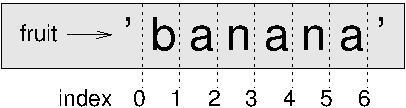
\includegraphics[scale=0.9]{../source/figs/banana.pdf}}
% \caption{Slice indices.}
\caption{切片索引。  }
\label{fig.banana}
\end{figure}

%🍁% If you omit the first index (before the colon), the slice starts at
%🍁% the beginning of the string.  If you omit the second index, the slice
%🍁% goes to the end of the string:

如果你省略第一个索引(冒号前面的值), 切片起始于字符串头部。  如果你省略第二个索引, 切片一直到字符串结尾:

\begin{lstlisting}
>>> fruit = 'banana'
>>> fruit[:3]
'ban'
>>> fruit[3:]
'ana'
\end{lstlisting}

%
%🍁% If the first index is greater than or equal to the second the result
%🍁% is an {\bf empty string}, represented by two quotation marks:
%🍁% \index{quotation mark}

如果第一个索引大于或等于第二个, 结果是 {\bf 空字符串}\footnote{empty string} , 用两个引号表示:

\begin{lstlisting}
>>> fruit = 'banana'
>>> fruit[3:3]
''
\end{lstlisting}

%
%🍁% An empty string contains no characters and has length 0, but other
%🍁% than that, it is the same as any other string.

一个空字符串不包括字符而且长度为 0, 但除此之外, 它和其它任何字符串一样。

%🍁% Continuing this example, what do you think
%🍁% {\tt fruit[:]} means?  Try it and see.
\index{copy!slice}  \index{slice!copy}
\index{复制!切片}  \index{切片!复制}

%🍁% \section{Strings are immutable  |  字符串是不可变的}
\section{字符串是不可变的}
\index{mutability}  \index{immutability}  \index{string!immutable}
\index{可变性}  \index{不可变性}  \index{字符串!不可变}

%🍁% It is tempting to use the {\tt []} operator on the left side of an
%🍁% assignment, with the intention of changing a character in a string.
%🍁% For example:
%🍁% \index{TypeError}  \index{exception!TypeError}

你会很想在赋值语句的左边使用 \li{[]}, 来改变字符串的一个字符。  例如:
\index{TypeError}  \index{exception!TypeError}

\begin{lstlisting}
>>> greeting = 'Hello, world!'
>>> greeting[0] = 'J'
TypeError: 'str' object does not support item assignment
\end{lstlisting}

%
%🍁% The ``object'' in this case is the string and the ``item'' is
%🍁% the character you tried to assign.  For now, an object is
%🍁% the same thing as a value, but we will refine that definition
%🍁% later (Section~\ref{equivalence}).
\index{object}  \index{item}  \index{item assignment}
\index{assignment!item}  \index{immutability}
\index{对象}  \index{元素}  \index{元素赋值}
\index{赋值!元素}  \index{不可变性}



错误信息中的 ``object (对象)'' 是那个字符串, ``item (元素)''是你要赋值的字符。  目前, 我们认为对象和值是同样的东西, 但是我们后面将改进此定义 (详见 \ref{equivalence}~节)。

%🍁% The reason for the error is that
%🍁% strings are {\bf immutable}, which means you can't change an
%🍁% existing string.  The best you can do is create a new string
%🍁% that is a variation on the original:

出现此错误的原因是字符串是 {\bf 不可变\footnote{immutable}的}, 这意味着你不能改变一个已存在的字符串。  你最多只能创建一个新的字符串, 在原有字符串的基础上略有变化:

\begin{lstlisting}
>>> greeting = 'Hello, world!'
>>> new_greeting = 'J' + greeting[1:]
>>> new_greeting
'Jello, world!'
\end{lstlisting}

%
%🍁% This example concatenates a new first letter onto
%🍁% a slice of {\tt greeting}.  It has no effect on
%🍁% the original string.
\index{concatenation}

上面的示例中, 我们将一个新的首字母拼接到 \li{greeting} 的一个切片上。  它不影响原字符串。


%🍁% \section{Searching  |  搜索}
\section{搜索}
\label{find}

%🍁% What does the following function do?
\index{find function}  \index{function!find}

下面的函数起什么作用?

\begin{lstlisting}
def find(word, letter):
    index = 0
    while index < len(word):
        if word[index] == letter:
            return index
        index = index + 1
    return -1
\end{lstlisting}

%
%🍁% In a sense, {\tt find} is the inverse of the {\tt []} operator.
%🍁% Instead of taking an index and extracting the corresponding character,
%🍁% it takes a character and finds the index where that character
%🍁% appears.  If the character is not found, the function returns {\tt
%🍁% -1}.

在某种意义上, \li{find} 和 \li{[]} 运算符相反。  与接受一个索引并提取相应的字符不同, 它接受一个字符并找到该字符所在的索引。  如果没有找到该字符, 函数返回 \li{-1}。

%🍁% This is the first example we have seen of a {\tt return} statement
%🍁% inside a loop.  If {\tt word[index] == letter}, the function breaks
%🍁% out of the loop and returns immediately.

这是我们第一次在循环内部看见 \li{return} 语句。  如果 \li{word[index] == letter},
函数停止循环并马上返回。

%🍁% If the character doesn't appear in the string, the program
%🍁% exits the loop normally and  returns {\tt -1}.

如果字符没出现在字符串中, 那么程序正常退出循环并返回 \li{-1}。

%🍁% This pattern of computation---traversing a sequence and returning
%🍁% when we find what we are looking for---is called a {\bf search}.
\index{traversal}  \index{search pattern}  \index{pattern!search}

这种计算模式——遍历一个序列并在找到寻找的东西时返回——被称作 {\em 搜索} (search)。

%🍁% As an exercise, modify {\tt find} so that it has a
%🍁% third parameter, the index in {\tt word} where it should start
%🍁% looking.

我们做个练习, 修改 \li {find} 函数使得它能接受第三个参数, 即从何处开始搜索的索引。

%🍁% \section{Looping and counting  |  循环和计数}
\section{循环和计数}
\label{counter}
\index{counter}  \index{counting and looping}
\index{looping and counting}  \index{looping!with strings}

%🍁% The following program counts the number of times the letter {\tt a}
%🍁% appears in a string:

下面的程序计算字母a在字符串中出现的次数:

\begin{lstlisting}
word = 'banana'
count = 0
for letter in word:
    if letter == 'a':
        count = count + 1
print(count)
\end{lstlisting}

%
%🍁% This program demonstrates another pattern of computation called a {\bf
%🍁% counter}.  The variable {\tt count} is initialized to 0 and then
%🍁% incremented each time an {\tt a} is found.
%🍁% When the loop exits, {\tt count}
%🍁% contains the result---the total number of {\tt a}'s.

此程序演示了另一种被称作 {\em 计数器} (counter) 的计算模式。  变量 \li{count} 初始化为 0 , 然后每次出现 \li{a} 时递增。  当循环结束时, \li{count} 包含了字母 \li{a} 出现的总次数。

\index{encapsulation}

%🍁% As an exercise, encapsulate this code in a function named {\tt
%🍁% count}, and generalize it so that it accepts the string and the
%🍁% letter as arguments.

\index{封装}
我们做一个练习, 将这段代码封装在一个名为 \li{count} 的函数中, 并泛化该函数, 使其接受字符串和字母作为实参。

%🍁% Then rewrite the function so that instead of
%🍁% traversing the string, it uses the three-parameter version of {\tt
%🍁% find} from the previous section.

然后重写这个函数, 不再使用字符串遍历, 而是使用上一节中三参数版本的 \li{find} 函数。

%🍁% \section{String methods  |  字符串方法}
\section{字符串方法}
\label{optional}

%🍁% Strings provide methods that perform a variety of useful operations.
%🍁% A method is similar to a function---it takes arguments and
%🍁% returns a value---but the syntax is different.  For example, the
%🍁% method {\tt upper} takes a string and returns a new string with
%🍁% all uppercase letters.
\index{method}  \index{string!method}

字符串提供了可执行多种有用操作的 {\em 方法} (method) 。  方法和函数类似, 接受实参并返回一个值, 但是语法不同。  例如, \li{upper} 方法接受一个字符串, 并返回一个都是大写字母的新字符串。
\index{方法}  \index{字符串!方法}

%🍁% Instead of the function syntax {\tt upper(word)}, it uses
%🍁% the method syntax {\tt word.upper()}.

不过使用的不是函数语法 \li{upper(word)} , 而是方法的语法 \li{word.upper()}。

\begin{lstlisting}
>>> word = 'banana'
>>> new_word = word.upper()
>>> new_word
'BANANA'
\end{lstlisting}

%
%🍁% This form of dot notation specifies the name of the method, {\tt
%🍁% upper}, and the name of the string to apply the method to, {\tt
%🍁% word}.  The empty parentheses indicate that this method takes no
%🍁% arguments.
\index{parentheses!empty}  \index{dot notation}

点标记法的形式指出方法的名字, \li{upper}, 以及应用该方法的字符串的名字, \li{word}。  空括号表明该方法不接受实参。

%🍁% A method call is called an {\bf invocation}; in this case, we would
%🍁% say that we are invoking {\tt upper} on {\tt word}.
\index{invocation}

这被称作 {\em 方法调用} (invocation); 此例中, 我们可以说是在 \li{word} 上调用 \li{upper} 。

%🍁% As it turns out, there is a string method named {\tt find} that
%🍁% is remarkably similar to the function we wrote:

事实上, 有一个被称为 \li{find} 的字符串方法, 与我们之前写的函数极其相似:

\begin{lstlisting}
>>> word = 'banana'
>>> index = word.find('a')
>>> index
1
\end{lstlisting}

%
%🍁% In this example, we invoke {\tt find} on {\tt word} and pass
%🍁% the letter we are looking for as a parameter.

此例中, 我们在 \li{word} 上调用 \li{find} , 并将我们要找的字母作为参数传入。

%🍁% Actually, the {\tt find} method is more general than our function;
%🍁% it can find substrings, not just characters

事实上, \li{find} 方法比我们的函数更通用; 它还可以查找子字符串, 而不仅仅是字符:

\begin{lstlisting}
>>> word.find('na')
2
\end{lstlisting}

%
%🍁% By default, {\tt find} starts at the beginning of the string, but
%🍁% it can take a second argument, the index where it should start:
\index{optional argument}  \index{argument!optional}

\li{find} 默认从字符串的首字母开始查找, 它还可以接受第二个实参, 即从何处开始的索引。

\begin{lstlisting}
>>> word.find('na', 3)
4
\end{lstlisting}

%
%🍁% This is an example of an {\bf optional argument};
%🍁% {\tt find} can
%🍁% also take a third argument, the index where it should stop:

这是一个 {\em 可选参数} (optional argument) 的例子; \li{find} 也可以接受结束查找的索引作为第三个实参:

\begin{lstlisting}
>>> name = 'bob'
>>> name.find('b', 1, 2)
-1
\end{lstlisting}

%
%🍁% This search fails because {\tt b} does not
%🍁% appear in the index range from {\tt 1} to {\tt 2}, not including {\tt
%🍁% 2}.  Searching up to, but not including, the second index makes
%🍁% {\tt find} consistent with the slice operator.

此次搜索失败, 因为 \li{'b'} 没有出现在索引 \li{1}--\li{2} 之间(不包括\li{2})。  一直搜索到第二个索引, 但是并不搜索第二个索引, 这使得 \li{find} 跟切片运算符的行为一致.

%🍁% \section{The {\tt in} operator  |  {\tt in} 运算符}
\section{{\tt in} 运算符}
\label{inboth}
\index{in operator}  \index{operator!in}
\index{boolean operator}  \index{operator!boolean}

%🍁% The word {\tt in} is a boolean operator that takes two strings and
%🍁% returns {\tt True} if the first appears as a substring in the second:

单词 \li{in} 是一个布尔运算符, 接受两个字符串。  如果第一个作为子串出现在第二个中, 则返回 \li{True}:

\begin{lstlisting}
>>> 'a' in 'banana'
True
>>> 'seed' in 'banana'
False
\end{lstlisting}

%
%🍁% For example, the following function prints all the
%🍁% letters from {\tt word1} that also appear in {\tt word2}:

例如, 下面的函数打印所有既出现在 \li{word1} 中, 也出现在 \li{word2} 中的字母:

\begin{lstlisting}
def in_both(word1, word2):
    for letter in word1:
        if letter in word2:
            print(letter)
\end{lstlisting}

%
%🍁% With well-chosen variable names,
%🍁% Python sometimes reads like English.  You could read
%🍁% this loop, ``for (each) letter in (the first) word, if (the) letter
%🍁% (appears) in (the second) word, print (the) letter.''

变量名挑选得当的话, Python 代码有时候读起来像是自然语言。  你可以这样读此循环, ``对于(每个) 在(第一个)单词中的字母, 如果(该)字母(出现)在(第二个)单词中, 打印(该)字母''。

%🍁% Here's what you get if you compare apples and oranges:

如果你比较 \li{'apples'} 和 \li{'oranges'}, 你会得到下面的结果:

\begin{lstlisting}
>>> in_both('apples', 'oranges')
a
e
s
\end{lstlisting}

%

%🍁% \section{String comparison  |  字符串比较}
\section{字符串比较}
\index{string!comparison}  \index{comparison!string}

%🍁% The relational operators work on strings.  To see if two strings are equal:

关系运算符也适用于字符串。  可以这样检查两个字符串是否相等:

\begin{lstlisting}
if word == 'banana':
    print('All right, bananas.')
\end{lstlisting}

%
%🍁% Other relational operations are useful for putting words in alphabetical
%🍁% order:

其它的关系运算符对于按字母序放置单词也很有用:

\begin{lstlisting}
if word < 'banana':
    print('Your word, ' + word + ', comes before banana.')
elif word > 'banana':
    print('Your word, ' + word + ', comes after banana.')
else:
    print('All right, bananas.')
\end{lstlisting}

%
%🍁% Python does not handle uppercase and lowercase letters the same way
%🍁% people do.  All the uppercase letters come before all the
%🍁% lowercase letters, so:

Python处理大写和小写字母的方式和人不同。  所有的大写字母出现在所有小写字母之前, 所以:

\begin{lstlisting}
Your word, Pineapple, comes before banana.
\end{lstlisting}

%
%🍁% A common way to address this problem is to convert strings to a
%🍁% standard format, such as all lowercase, before performing the
%🍁% comparison. Keep that in mind in case you have to defend yourself
%🍁% against a man armed with a Pineapple.

%🍁% \section{Debugging  |  调试}
\section{调试}
\index{debugging}  \index{traversal}
\index{调试}  \index{遍历}

%🍁% When you use indices to traverse the values in a sequence,
%🍁% it is tricky to get the beginning and end of the traversal
%🍁% right.  Here is a function that is supposed to compare two
%🍁% words and return {\tt True} if one of the words is the reverse
%🍁% of the other, but it contains two errors:

当你使用索引遍历序列中的值时, 正确地指定遍历的起始和结束点有点困难。  下面是一个用来比较两个单词的函数, 如果一个单词是另一个的倒序, 则返回 \li{True} , 但其中有两个错误:

\begin{lstlisting}
def is_reverse(word1, word2):
    if len(word1) != len(word2):
        return False

    i = 0
    j = len(word2)

    while j > 0:
        if word1[i] != word2[j]:
            return False
        i = i+1
        j = j-1

    return True
\end{lstlisting}

%
%🍁% The first {\tt if} statement checks whether the words are the
%🍁% same length.  If not, we can return {\tt False} immediately.
%🍁% Otherwise, for the rest of the function, we can assume that the words
%🍁% are the same length.  This is an example of the guardian pattern
%🍁% in Section~\ref{guardian}.
\index{guardian pattern}  \index{pattern!guardian}
\index{index}
\index{监护人模式}  \index{模式!监护人}
\index{索引}

第一条 \li{if} 语句检查两个单词是否等长。  如果不是, 我们可以马上返回 \li{False} 。  否则, 在函数其余的部分, 我们可以假定单词是等长的。  这是~\ref{guardian}节中提到的监护人模式的一个例子。

%🍁% {\tt i} and {\tt j} are indices: {\tt i} traverses {\tt word1}
%🍁% forward while {\tt j} traverses {\tt word2} backward.  If we find
%🍁% two letters that don't match, we can return {\tt False} immediately.
%🍁% If we get through the whole loop and all the letters match, we
%🍁% return {\tt True}.

\li{i} 和 \li{j} 是索引:\li{i} 向前遍历 \li{word1}, \li{j} 向后遍历 \li{word2}。  如果我们找到两个不匹配的字母, 我们可以立即返回 \li{False}。  如果我们完成整个循环并且所有字母都匹配, 我们返回 \li{True} 。

%🍁% If we test this function with the words ``pots'' and ``stop'', we
%🍁% expect the return value {\tt True}, but we get an IndexError:
\index{IndexError}  \index{exception!IndexError}

如果我们用单词 ``pots'' 和 ``stop'' 测试该函数, 我们期望返回 \li{True} , 但是却得到一个 \li{IndexError}:

\begin{lstlisting}
>>> is_reverse('pots', 'stop')
...
  File "reverse.py", line 15, in is_reverse
    if word1[i] != word2[j]:
IndexError: string index out of range
\end{lstlisting}

%
%🍁% For debugging this kind of error, my first move is to
%🍁% print the values of the indices immediately before the line
%🍁% where the error appears.

为了调试该类错误, 我第一步是在错误出现的行之前, 打印索引的值。

\begin{lstlisting}
    while j > 0:
        print(i, j)        # print here

        if word1[i] != word2[j]:
            return False
        i = i+1
        j = j-1
\end{lstlisting}

%
%🍁% Now when I run the program again, I get more information:

现在, 当我再次运行该程序时, 将获得更多的信息:

\begin{lstlisting}
>>> is_reverse('pots', 'stop')
0 4
...
IndexError: string index out of range
\end{lstlisting}

%
%🍁% The first time through the loop, the value of {\tt j} is 4,
%🍁% which is out of range for the string \verb"'pots'".
%🍁% The index of the last character is 3, so the
%🍁% initial value for {\tt j} should be {\tt len(word2)-1}.

第一次循环时, \li{j} 的值是4, 超出字符串 \li{'post'} 的范围了。  最后一个字符的索引是 \li{3}, 所以 \li{j} 的初始值应该是 \li{len(word2)-1} 。

%🍁% If I fix that error and run the program again, I get:

如果我解决了这个错误, 然后运行程序, 将获得如下输出:

\begin{lstlisting}
>>> is_reverse('pots', 'stop')
0 3
1 2
2 1
True
\end{lstlisting}

%
%🍁% This time we get the right answer, but it looks like the loop only ran
%🍁% three times, which is suspicious.  To get a better idea of what is
%🍁% happening, it is useful to draw a state diagram.  During the first
%🍁% iteration, the frame for \verb"is_reverse" is shown in
%🍁% Figure~\ref{fig.state4}.  \index{state diagram} \index{diagram!state}

这次我们获得了正确的答案, 但是看起来循环只运行了三次, 这很奇怪。  画栈图可以帮我们更好的理解发生了什么。  在第一次迭代期间, \li{is_reverse} 的栈帧如图~\ref{fig.state4} 所示。

\begin{figure}
\centerline
{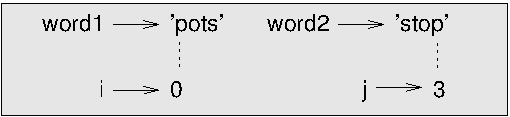
\includegraphics[scale=0.8]{../source/figs/state4.pdf}}
% \caption{State diagram.}
\caption{堆栈图。  }
\label{fig.state4}
\end{figure}

%🍁% I took some license by arranging the variables in the frame
%🍁% and adding dotted lines to show that the values of {\tt i} and
%🍁% {\tt j} indicate characters in {\tt word1} and {\tt word2}.

我对堆栈图做了些调整, 重新排列了栈帧中的变量, 增加了虚线来说明 \li{i} 和 \li{j} 的值表示 \li{word1} 和 \li{word2} 中的字符。


%🍁% Starting with this diagram, run the program on paper, changing the
%🍁% values of {\tt i} and {\tt j} during each iteration.  Find and fix the
%🍁% second error in this function.

从这个堆栈图开始, 在纸上运行程序, 每次迭代时修改 \li{i} 和 \li{j} 的值。  查找并解决这个函数的中第二个错误。
\label{isreverse}


%🍁% \section{Glossary  |  术语表}
\section{术语表}

%🍁% \begin{description}
%🍁%
%🍁% \item[object:] Something a variable can refer to.  For now,
%🍁% you can use ``object'' and ``value'' interchangeably.
%🍁% \index{object}
%🍁%
%🍁% \item[sequence:] An ordered collection of
%🍁% values where each value is identified by an integer index.
%🍁% \index{sequence}
%🍁%
%🍁% \item[item:] One of the values in a sequence.
%🍁% \index{item}
%🍁%
%🍁% \item[index:] An integer value used to select an item in
%🍁% a sequence, such as a character in a string.  In Python
%🍁% indices start from 0.
%🍁% \index{index}
%🍁%
%🍁% \item[slice:] A part of a string specified by a range of indices.
%🍁% \index{slice}
%🍁%
%🍁% \item[empty string:] A string with no characters and length 0, represented
%🍁% by two quotation marks.
%🍁% \index{empty string}
%🍁%
%🍁% \item[immutable:] The property of a sequence whose items cannot
%🍁% be changed.
%🍁% \index{immutability}
%🍁%
%🍁% \item[traverse:] To iterate through the items in a sequence,
%🍁% performing a similar operation on each.
%🍁% \index{traversal}
%🍁%
%🍁% \item[search:] A pattern of traversal that stops
%🍁% when it finds what it is looking for.
%🍁% \index{search pattern}
%🍁% \index{pattern!search}
%🍁%
%🍁% \item[counter:] A variable used to count something, usually initialized
%🍁% to zero and then incremented.
%🍁% \index{counter}
%🍁%
%🍁% \item[invocation:] A statement that calls a method.
%🍁% \index{invocation}
%🍁%
%🍁% \item[optional argument:] A function or method argument that is not
%🍁% required.
%🍁% \index{optional argument}
%🍁% \index{argument!optional}
%🍁%
%🍁% \end{description}

\begin{description}

\item[对象 (object):] 变量可以引用的东西。  现在你将对象和值等价使用。
\index{object}

\item[序列 (sequence):] 一个有序的值的集合, 每个值通过一个整数索引标识。
\index{sequence}

\item[元素 (item):] 序列中的一个值。
\index{item}

\item[索引 (index):] 用来选择序列中元素 (如字符串中的字符) 的一个整数值。  在Python中, 索引从0开始。
\index{index}

\item[切片 (slice):] 以索引范围指定的字符串片段。
\index{slice}

\item[空字符串 (empty string):] 一个没有字符的字符串, 长度为0, 用两个引号表示。
\index{empty string}

\item[不可变性 (immutable)] 元素不能被改变的序列的性质。
\index{immutability}

\item[遍历 (traversal):] 对一个序列的所有元素进行迭代, 对每一元素执行类似操作。
\index{traversal}

\item[搜索 (search):] 一种遍历模式, 当找到搜索目标时就停止。
\index{search pattern}  \index{pattern!search}

\item[计数器 (counter):] 用来计数的变量, 通常初始化为0, 并以此递增。
\index{counter}

\item[方法调用(invocation):] 执行一个方法的声明.
\index{invocation}

\item[可选参数 (optional argument):] 一个函数或者一个方法中不必要指定的参数。
\index{optional argument}  \index{argument!optional}

\end{description}


%🍁% \section{Exercises  |  练习}
\section{练习}

\begin{exercise}
\index{string method}  \index{method!string}

%🍁% Read the documentation of the string methods at
%🍁% \url{http://docs.python.org/3/library/stdtypes.html#string-methods}.
%🍁% You might want to experiment with some of them to make sure you
%🍁% understand how they work.  {\tt strip} and {\tt replace} are
%🍁% particularly useful.

点击如下链接, 阅读\href{http://docs.python.org/3/library/stdtypes.html#string-methods}{字符串方法}的文档。   为了确保你理解他们是怎么工作的, 可以尝试使用其中的一些方法。  {\em \li{strip}} 和 {\em \li{replace}} 尤其有用。

%🍁% The documentation uses a syntax that might be confusing.
%🍁% For example, in \verb"find(sub[, start[, end]])", the brackets
%🍁% indicate optional arguments.  So {\tt sub} is required, but
%🍁% {\tt start} is optional, and if you include {\tt start},
%🍁% then {\tt end} is optional.

文档中使用了可能会引起困惑的句法。  例如, 在 {\em \li{find(sub[, start[, end]])}} 中, 方括号意味着这是可选参数。  所以, {\em \li{sub}} 是必填参数, 但是 {\em \li{start}} 是可选的, 而且如果你提供了 {\em \li{start}} , 也不一定必须提供 {\em \li{end}} 。

\index{optional argument}  \index{argument!optional}

\end{exercise}


\begin{exercise}
\index{count method}  \index{method!count}

%🍁% There is a string method called {\tt count} that is similar
%🍁% to the function in Section~\ref{counter}.  Read the documentation
%🍁% of this method
%🍁% and write an invocation that counts the number of {\tt a}'s
%🍁% in \verb"'banana'".

有一个字符串方法叫 {\em \li{count}} , 它类似于之前 {\em \ref{counter}}~节中的 {\em \li{counter}} 。  阅读这个方法的文档, 写一个计算 {\em \li{'banana'}} 中 {\em \li{a}} 的个数的方法调用。


\end{exercise}


\begin{exercise}
\index{step size}  \index{slice operator}  \index{operator!slice}
\index{步长}  \index{切片操作}  \index{操作!切片}

%🍁% A string slice can take a third index that specifies the ``step
%🍁% size''; that is, the number of spaces between successive characters.
%🍁% A step size of 2 means every other character; 3 means every third,
%🍁% etc.

一个字符串切片可以接受指定步长的第三个索引; 也就是连续字符间空格的个数。  步长为{\em 2}, 意味着每隔一个字符;步长为{\em 3}, 意味着每隔两个字符, 以此类推。

\begin{lstlisting}
>>> fruit = 'banana'
>>> fruit[0:5:2]
'bnn'
\end{lstlisting}

%🍁% A step size of -1 goes through the word backwards, so
%🍁% the slice \verb"[::-1]" generates a reversed string.
\index{palindrome}

步长为 {\em \li{-1}} 就是从单词的尾部开始进行, 所以切片 {\em \li{[::-1]}} 生成一个倒序的字符串。

%🍁% Use this idiom to write a one-line version of \verb"is_palindrome"
%🍁% from Exercise~\ref{palindrome}.

利用这个习惯用法\footnote{idiom}, 将习题~{\em \ref{palindrome}}中 {\em \li{is_palindrome}} 函数改写为一行代码版。

\end{exercise}

\begin{exercise}

%🍁% The following functions are all {\em intended} to check whether a
%🍁% string contains any lowercase letters, but at least some of them are
%🍁% wrong.  For each function, describe what the function actually does
%🍁% (assuming that the parameter is a string).

下面这些函数, 都是 {\bf 用于} 检查一个字符串是否包含一些小写字母的, 但是其中至少有一些是错误的函数。  检查每个函数, 描述这个函数实际上做了什么 {\em (} 假设形参是字符串{\em )}。

\begin{em}
\begin{lstlisting}
def any_lowercase1(s):
    for c in s:
        if c.islower():
            return True
        else:
            return False

def any_lowercase2(s):
    for c in s:
        if 'c'.islower():
            return 'True'
        else:
            return 'False'

def any_lowercase3(s):
    for c in s:
        flag = c.islower()
    return flag

def any_lowercase4(s):
    flag = False
    for c in s:
        flag = flag or c.islower()
    return flag

def any_lowercase5(s):
    for c in s:
        if not c.islower():
            return False
    return True
\end{lstlisting}
\end{em}

\end{exercise}


\begin{exercise}
\index{letter rotation}  \index{rotation, letter}
\index{字母偏移}

\label{exrotate}
%🍁% A Caesar cypher is a weak form of encryption that involves ``rotating'' each
%🍁% letter by a fixed number of places.  To rotate a letter means
%🍁% to shift it through the alphabet, wrapping around to the beginning if
%🍁% necessary, so 'A' rotated by 3 is 'D' and 'Z' rotated by 1 is 'A'.

凯撒密码 {\em (Caesar cypher)} 是一种弱加密方式, 它将每一个字母偏移固定的位置。  偏移一个字母, 指的是按着字母表偏移, 如果需要的话再从尾部跳转至首字母, 所以 {\em `A'} 偏移三个位置即为 {\em `D'}, {\em `Z'} 偏移一个位置是 {\em `A'}。
% chn transplation need imporve

%🍁% To rotate a word, rotate each letter by the same amount.
%🍁% For example, ``cheer'' rotated by 7 is ``jolly'' and ``melon'' rotated
%🍁% by -10 is ``cubed''.  In the movie {\em 2001: A Space Odyssey}, the
%🍁% ship computer is called HAL, which is IBM rotated by -1.

要偏移一个单词, 可以将其中每一个字母偏移相同的量。  例如, {\em ``cheer''} 偏移 {\em 7} 个位置后变成了 {\em ``jolly''}, {\em ``melon''} 偏移 {\em -10} 个位置变成了 {\em ``cubed''}。  在电影 {\em 《2001:}太空奥德赛{\em (2001: A Space Odyssey)》} 中, 飞船上的电脑叫做 {\em HAL}, 也就是 {\em IBM} 偏移 {\em 1} 个位置后的单词。

%For example ``sleep''
%rotated by 9 is ``bunny'' and ``latex'' rotated by 7 is ``shale''.

%🍁% Write a function called \verb"rotate_word"
%🍁% that takes a string and an integer as parameters, and returns
%🍁% a new string that contains the letters from the original string
%🍁% rotated by the given amount.

编写一个叫 {\em \li{rotate_word}} 的函数, 接受一个字符串和一个整数作为形参, 并返回原字符串按照给定整数量偏移后得到的一个新字符串。

%🍁% You might want to use the built-in function {\tt ord}, which converts
%🍁% a character to a numeric code, and {\tt chr}, which converts numeric
%🍁% codes to characters.  Letters of the alphabet are encoded in alphabetical
%🍁% order, so for example:

你可能想用内置函数 {\em \li{ord}} , 它可以将字符转化成数值代码, 还有 {\em \li{chr}}, 它可以将数值代码转化成字符. 字母表的字母以字母表顺序编码, 例如:

\begin{em}
\begin{lstlisting}
>>> ord('c') - ord('a')
2
\end{lstlisting}
\end{em}

%🍁% Because \verb"'c'" is the two-eth letter of the alphabet.  But
%🍁% beware: the numeric codes for upper case letters are different.

因为 {\em \li{'c'}} 是字母表中的第二个字母。  但是请注意:大写字母的数值代码是不同的。

%🍁% Potentially offensive jokes on the Internet are sometimes encoded in
%🍁% ROT13, which is a Caesar cypher with rotation 13.  If you are not
%🍁% easily offended, find and decode some of them.  Solution:
%🍁% \url{http://thinkpython2.com/code/rotate.py}.

网上一些可能冒犯人的笑话有时以 {\em ROT13} 编码, 即以 {\em 13} 为偏移量的凯撒
密码。  如果你不是很容易就被冒犯, 那么可以找些这样的笑话, 并解码。

\href{http://thinkpython2.com/code/rotate.py}{参考答案}

\end{exercise}



%🍁% \chapter{Case study: word play  |  文字游戏}
\chapter{案例研究:文字游戏}
\label{wordplay}

%🍁% This chapter presents the second case study, which involves
%🍁% solving word puzzles by searching for words that have certain
%🍁% properties.  For example, we'll find the longest palindromes
%🍁% in English and search for words whose letters appear in
%🍁% alphabetical order.  And I will present another program development
%🍁% plan: reduction to a previously solved problem.

这一章将介绍第二个案例研究, 即通过查找具有特定属性的单词来解答字谜游戏。
例如, 我们将找出英文中最长的回文单词, 以及字符按照字符表顺序出现的单词。
另外, 我还将介绍另一种程序开发方法: 简化为之前已解决的问题。

%🍁% \section{Reading word lists  |  读取单词列表}
\section{读取单词列表}
\label{wordlist}

%🍁% For the exercises in this chapter we need a list of English words.
%🍁% There are lots of word lists available on the Web, but the one most
%🍁% suitable for our purpose is one of the word lists collected and
%🍁% contributed to the public domain by Grady Ward as part of the Moby
%🍁% lexicon project (see \url{http://wikipedia.org/wiki/Moby_Project}).  It
%🍁% is a list of 113,809 official crosswords; that is, words that are
%🍁% considered valid in crossword puzzles and other word games.  In the
%🍁% Moby collection, the filename is {\tt 113809of.fic}; you can download
%🍁% a copy, with the simpler name {\tt words.txt}, from
%🍁% \url{http://thinkpython2.com/code/words.txt}.
\index{Moby Project}  \index{crosswords}

为了完成本章的习题, 我们需要一个英语单词的列表。
网络上有许多单词列表, 但是最符合我们目的列表之一是由 Grady
Ward收集并贡献给公众的列表, 这也是Moby词典项目的一部分\footnote{(见:\url{http://wikipedia.org/wiki/Moby_Project}}。
它由 113,809 个填字游戏单词组成, 即在填字游戏以及其它文字游戏中被认为有效的单词。
在 Moby 集合中, 该列表的文件名是 \li{113809of.fic} ;你可以从 \href{http://thinkpython.com/code/words.txt}{这里} 下载一个拷贝, 文件名已被简化为 \li{words.txt}。

\index{Moby Project}  \index{crosswords}
\index{维基百科}

%🍁% This file is in plain text, so you can open it with a text
%🍁% editor, but you can also read it from Python.  The built-in
%🍁% function {\tt open} takes the name of the file as a parameter
%🍁% and returns a {\bf file object} you can use to read the file.

该文件是纯文本, 因此你可以用一个文本编辑器打开它, 但是你也可以从 Python 中读取它。   内建函数 \li{open} 接受文件名作为形参, 并返回一个 {\em 文件对象} (file object), 你可以使用它读取该文件。

\index{open function}  \index{function!open}
\index{plain text}  \index{text!plain}
\index{object!file}  \index{file object}

\begin{lstlisting}
>>> fin = open('words.txt')
\end{lstlisting}

%🍁% %
%🍁% {\tt fin} is a common name for a file object used for input.  The file
%🍁% object provides several methods for reading, including {\tt readline},
%🍁% which reads characters from the file until it gets to a newline and
%🍁% returns the result as a string:
\index{readline method}  \index{method!readline}
\index{readline 方法}  \index{方法!readline}

\li{`fin} 是输入文件对象的一个常用名。
该文件对象提供了几个读取方法, 包括 \li{readline}, 其从文件中读取字符直到碰到新行, 并将结果作为字符串返回:
\index{method!readline}

\begin{lstlisting}
>>> fin.readline()
'aa\r\n'
\end{lstlisting}

%🍁% %
%🍁% The first word in this particular list is ``aa'', which is a kind of
%🍁% lava.  The sequence \verb"\r\n" represents two whitespace characters,
%🍁% a carriage return and a newline, that separate this word from the
%🍁% next.

在此列表中, 第一个单词是 ``aa'', 它是一类熔岩的名称。   序列 \li{\r\n} 代表两个空白字符, 回车和换行, 它们将这个单词和下一个分开。

%🍁% The file object keeps track of where it is in the file, so
%🍁% if you call {\tt readline} again, you get the next word:

此文件对象跟踪它在文件中的位置,
所以如果你再次调用 \li{readline}, 你获得下一个单词:

\begin{lstlisting}
>>> fin.readline()
'aah\r\n'
\end{lstlisting}

%🍁% %
%🍁% The next word is ``aah'', which is a perfectly legitimate
%🍁% word, so stop looking at me like that.
%🍁% Or, if it's the whitespace that's bothering you,
%🍁% we can get rid of it with the string method {\tt strip}:

下一个单词是 ``aah'', 不要惊讶, 它是一个完全合法的单词。
或者, 如果空格困扰了你, 我们可以用字符串方法 \li{strip} 删掉它:
\index{strip method}  \index{method!strip}
\index{strip 方法}  \index{方法!strip}


\begin{lstlisting}
>>> line = fin.readline()
>>> word = line.strip()
>>> word
'aahed'
\end{lstlisting}

%🍁% %
%🍁% You can also use a file object as part of a {\tt for} loop.
%🍁% This program reads {\tt words.txt} and prints each word, one
%🍁% per line:

你也可以将文件对象用做 \li{for} 循环的一部分。
此程序读取 \li{words.txt} 并打印每个单词, 每行一个:
\index{open function}  \index{function!open}

\begin{lstlisting}
fin = open('words.txt')
for line in fin:
    word = line.strip()
    print(word)
\end{lstlisting}

%
%🍁% \section{Exercises  |  练习}
\section{练习}

%🍁% There are solutions to these exercises in the next section.
%🍁% You should at least attempt each one before you read the solutions.

\hyperref[search]{下一节}将给出了这些习题的答案。
在你看答案之前, 应该试着解答一下。

\begin{exercise}
%🍁% Write a program that reads {\tt words.txt} and prints only the
%🍁% words with more than 20 characters (not counting whitespace).

编程写一个程序, 使得它可以读取 {\em \li{words.txt}} , 然后只打印出那些长度超过 20 个字符的单词 (不包括空格)。
\index{whitespace}

\end{exercise}

\begin{exercise}

%🍁% In 1939 Ernest Vincent Wright published a 50,000 word novel called
%🍁% {\em Gadsby} that does not contain the letter ``e''.  Since ``e'' is
%🍁% the most common letter in English, that's not easy to do.

{\em 1939} 年, {\em Ernest Vincent Wright} 出版了一本名为 {\em 《Gadsby》} 的小说,
该小说里完全没有使用字符 {\em ``e''}。   由于 {\em ``e''} 是英文中最常用的字符, 因此写出这本书并不容易。

%🍁% In fact, it is difficult to construct a solitary thought without using
%🍁% that most common symbol.  It is slow going at first, but with caution
%🍁% and hours of training you can gradually gain facility.

事实上, 不使用这个最常用的字符来构建一个简单的想法都是很难的。
开始进展缓慢, 但是经过有意识的、长时间的训练, 你可以逐渐地熟练。

%🍁% All right, I'll stop now.

好啦, 不说题外话了, 我们开始编程练习。

%🍁% Write a function called \verb"has_no_e" that returns {\tt True} if
%🍁% the given word doesn't have the letter ``e'' in it.

写一个叫做 {\em \li{has_no_e}} 的函数, 如果给定的单词中不包含字符 {\em ``e''}, 返回 {\em \li{True}} 。

%🍁% Modify your program from the previous section to print only the words
%🍁% that have no ``e'' and compute the percentage of the words in the list
%🍁% that have no ``e''.

修改上一节中的程序, 只打印不包含 {\em ``e''} 的单词, 并且计算列表中不含 {\em ``e''} 单词的比例。
\index{lipogram}

\end{exercise}


\begin{exercise}

%🍁% Write a function named {\tt avoids}
%🍁% that takes a word and a string of forbidden letters, and
%🍁% that returns {\tt True} if the word doesn't use any of the forbidden
%🍁% letters.

编写一个名为 {\em \li{avoids}} 的函数, 接受一个单词和一个指定禁止使用字符的字符串,
如果单词中不包含任意被禁止的字符, 则返回 {\em \li{True}} 。

%🍁% Modify your program to prompt the user to enter a string
%🍁% of forbidden letters and then print the number of words that
%🍁% don't contain any of them.
%🍁% Can you find a combination of 5 forbidden letters that
%🍁% excludes the smallest number of words?

修改你的程序, 提示用户输入一个禁止使用的字符, 然后打印不包含这些字符的单词的数量。
你能找到一个5个禁止使用字符的组合, 使得其排除的单词数目最少么?

\end{exercise}



\begin{exercise}

%🍁% Write a function named \verb"uses_only" that takes a word and a
%🍁% string of letters, and that returns {\tt True} if the word contains
%🍁% only letters in the list.  Can you make a sentence using only the
%🍁% letters {\tt acefhlo}?  Other than ``Hoe alfalfa?''

编写一个名为 {\em \li{uses_only}} 的函数, 接受一个单词和一个字符串。
如果该单词只包括此字符串中的字符, 则返回 {\em \li{True}}。
你能只用 {\em \li{"acefhlo"}} 这几个字符造一个句子么? 除了 ``Hoe alfalfa'' 外。

\end{exercise}


\begin{exercise}

%🍁% Write a function named \verb"uses_all" that takes a word and a
%🍁% string of required letters, and that returns {\tt True} if the word
%🍁% uses all the required letters at least once.  How many words are there
%🍁% that use all the vowels {\tt aeiou}?  How about {\tt aeiouy}?

编写一个名为 {\em \li{uses_all}} 的函数, 接受一个单词和一个必须使用的字符组成的字符串。
如果该单词包括此字符串中的全部字符至少一次, 则返回 {\em \li{True}}。
你能统计出多少单词包含了所有的元音字符 {\em \li{aeiou}}吗?如果换成 {\em \li{aeiouy}} 呢?

\end{exercise}


\begin{exercise}

%🍁% Write a function called \verb"is_abecedarian" that returns
%🍁% {\tt True} if the letters in a word appear in alphabetical order
%🍁% (double letters are ok).
%🍁% How many abecedarian words are there?

编写一个名为 {\em \li{is_abecedarian}} 的函数, 如果单词中的字符以字符表的顺序出现(允许重复字符), 则返回 {\em \li{True}} 。
有多少个具备这种特征的单词?

\index{abecedarian}  \index{字符表}

\end{exercise}



%🍁% \section{Search  ||  搜索}
\section{搜索}
\label{search}
\index{search pattern}  \index{pattern!search}

%🍁% All of the exercises in the previous section have something
%🍁% in common; they can be solved with the search pattern we saw
%🍁% in Section~\ref{find}.  The simplest example is:

前一节的所有习题有一个共同点;都可以用在 \ref{find}~节 中看到的搜索模式解决。

\begin{lstlisting}
def has_no_e(word):
    for letter in word:
        if letter == 'e':
            return False
    return True
\end{lstlisting}

%
%🍁% The {\tt for} loop traverses the characters in {\tt word}.  If we find
%🍁% the letter ``e'', we can immediately return {\tt False}; otherwise we
%🍁% have to go to the next letter.  If we exit the loop normally, that
%🍁% means we didn't find an ``e'', so we return {\tt True}.

\li{for} 循环遍历 \li{word} 中的字符。
如果我们找到字符 \li{"e"}, 那么我们可以马上返回 \li{False} ;
否则我们必须检查下一个字符。
如果我们正常退出循环, 就意味着我们没有找到一个 ``e'', 所以我们返回 \li{True} 。

\index{traversal}

\index{in operator}  \index{operator!in}

%🍁% You could write this function more concisely using the {\tt in}
%🍁% operator, but I started with this version because it
%🍁% demonstrates the logic of the search pattern.

你也可以用 \li{in} 操作符简化上述函数, 但之所以一开始写成这样, 是因为它展示了搜索模式的逻辑。

\index{generalization}

%🍁% {\tt avoids} is a more general version of \verb"has_no_e" but it
%🍁% has the same structure:

\li{avoid} 是一个更通用的 \li{has_no_e} 函数, 但是结构是相同的:

\begin{lstlisting}
def avoids(word, forbidden):
    for letter in word:
        if letter in forbidden:
            return False
    return True
\end{lstlisting}

%🍁% %
%🍁% We can return {\tt False} as soon as we find a forbidden letter;
%🍁% if we get to the end of the loop, we return {\tt True}.

一旦我们找到一个禁止使用的字符, 我们返回 \li{False} ;
如果我们到达循环结尾, 我们返回 \li{True} 。

%🍁% \verb"uses_only" is similar except that the sense of the condition
%🍁% is reversed:

除了检测条件相反以外, 下面 \li{uses_only} 函数与上面的函数很像:

\begin{lstlisting}
def uses_only(word, available):
    for letter in word:
        if letter not in available:
            return False
    return True
\end{lstlisting}

%🍁% %
%🍁% Instead of a list of forbidden letters, we have a list of available
%🍁% letters.  If we find a letter in {\tt word} that is not in
%🍁% {\tt available}, we can return {\tt False}.

这里我们传入一个允许使用字符的列表, 而不是禁止使用字符的列表。
如果我们在 \li{word} 中找到一个不在 \li{available} 中的字符, 我们就可以返回 \li{False} 。

%🍁% \verb"uses_all" is similar except that we reverse the role
%🍁% of the word and the string of letters:

除了将 \li{word} 与所要求的字符的角色进行了调换之外,
下面的 \li{uses_all} 函数也是类似的。

\begin{lstlisting}
def uses_all(word, required):
    for letter in required:
        if letter not in word:
            return False
    return True
\end{lstlisting}

%🍁% %
%🍁% Instead of traversing the letters in {\tt word}, the loop
%🍁% traverses the required letters.  If any of the required letters
%🍁% do not appear in the word, we can return {\tt False}.

该循环遍历需要的字符, 而不是遍历 \li{word} 中的字符。  如果任何要求的字符没出现在单词中, 则我们返回 \li{False} 。

\index{traversal}

%🍁% If you were really thinking like a computer scientist, you would
%🍁% have recognized that \verb"uses_all" was an instance of a
%🍁% previously solved problem, and you would have written:

如果你真的像计算机科学家一样思考, 你可能已经意识到 \li{uses_all} 是前面已经解决的问题的一个实例, 你可能会写成:

\begin{lstlisting}
def uses_all(word, required):
    return uses_only(required, word)
\end{lstlisting}

%🍁% %
%🍁% This is an example of a program development plan called {\bf
%🍁%   reduction to a previously solved problem}, which means that you
%🍁% recognize the problem you are working on as an instance of a solved
%🍁% problem and apply an existing solution.  \index{reduction to a
%🍁%   previously solved problem} \index{development plan!reduction}

这是一种叫做 {\bf 简化为之前已解决的问题\footnote{reduction to a
previously solved problem}} 的程序开发方法的一个示例,
也就是说, 你认识到当前面临的问题是之前已经解决的问题的一个实例,
然后应用了已有的解决方案。


%🍁% \section{Looping with indices  |  使用索引进行循环}
\section{使用索引进行循环}
\index{looping!with indices}  \index{index!looping with}
\index{循环!使用索引}  \index{索引!控制循环}

%🍁% I wrote the functions in the previous section with {\tt for}
%🍁% loops because I only needed the characters in the strings; I didn't
%🍁% have to do anything with the indices.

前一节我用 \li{for} 循环来编写函数, 因为我只需要处理字符串中的字符;
我不必用索引做任

%🍁% For \verb"is_abecedarian" we have to compare adjacent letters,
%🍁% which is a little tricky with a {\tt for} loop:

对于下面的 \li{is_abecedarian} , 我们必须比较邻接的字符, 用 \li{for} 循环来写的话有点棘手。

\begin{lstlisting}
def is_abecedarian(word):
    previous = word[0]
    for c in word:
        if c < previous:
            return False
        previous = c
    return True
\end{lstlisting}

%🍁% An alternative is to use recursion:

一种替代方法是使用递归:

\begin{lstlisting}
def is_abecedarian(word):
    if len(word) <= 1:
        return True
    if word[0] > word[1]:
        return False
    return is_abecedarian(word[1:])
\end{lstlisting}

%🍁% Another option is to use a {\tt while} loop:

另一中方法是使用 \li{while} 循环:

\begin{lstlisting}
def is_abecedarian(word):
    i = 0
    while i < len(word)-1:
        if word[i+1] < word[i]:
            return False
        i = i+1
    return True
\end{lstlisting}

%🍁% %
%🍁% The loop starts at {\tt i=0} and ends when {\tt i=len(word)-1}.  Each
%🍁% time through the loop, it compares the $i$th character (which you can
%🍁% think of as the current character) to the $i+1$th character (which you
%🍁% can think of as the next).

循环起始于 \li{i=0} , \li{i=len(word)-1} 时结束。
每次循环, 函数会比较第 $i$ 个字符(可以将其认为是当前字符)
和第 $i+1$ 个字符(可以将其认为是下一个字符)。

%🍁% If the next character is less than (alphabetically before) the current
%🍁% one, then we have discovered a break in the abecedarian trend, and
%🍁% we return {\tt False}.

如果下一个字符比当前的小(字符序靠前),
那么我们在递增趋势中找到了断点, 即可返回 \li{False} 。

%🍁% If we get to the end of the loop without finding a fault, then the
%🍁% word passes the test.  To convince yourself that the loop ends
%🍁% correctly, consider an example like \verb"'flossy'".  The
%🍁% length of the word is 6, so
%🍁% the last time the loop runs is when {\tt i} is 4, which is the
%🍁% index of the second-to-last character.  On the last iteration,
%🍁% it compares the second-to-last character to the last, which is
%🍁% what we want.

如果到循环结束时我们也没有找到一点错误, 那么该单词通过测试。
为了让你相信循环正确地结束了, 我们用 \li{'flossy'} 这个单词来举例。
它的长度为 6, 因此最后一次循环运行时, \li{i} 是 4, 这是倒数第 2 个字符的索引。
最后一次迭代时, 函数比较倒数第二个和最后一个字符, 这正是我们希望的。
\index{palindrome}

%🍁% Here is a version of \verb"is_palindrome" (see
%🍁% Exercise~\ref{palindrome}) that uses two indices; one starts at the
%🍁% beginning and goes up; the other starts at the end and goes down.

下面是 \li{is_palindrome} 函数的一种版本(详见 练习~\ref{palindrome} )
, 其中使用了两个索引;一个从最前面开始并往前上, 另一个从最后面开始并往下走。

\begin{lstlisting}
def is_palindrome(word):
    i = 0
    j = len(word)-1

    while i<j:
        if word[i] != word[j]:
            return False
        i = i+1
        j = j-1

    return True
\end{lstlisting}

%🍁% Or we could reduce to a previously solved
%🍁% problem and write:

或者, 我们可以把问题简化为之前已经解决的问题, 这样来写:

\index{reduction to a previously solved problem}
\index{development plan!reduction}

\begin{lstlisting}
def is_palindrome(word):
    return is_reverse(word, word)
\end{lstlisting}

%🍁% %
%🍁% Using \verb"is_reverse" from Section~\ref{isreverse}.

使用 \ref{isreverse}~节 中描述的 \li{is_reverse}


%🍁% \section{Debugging  |  调试}
\section{调试}
\index{debugging}  \index{testing!is hard}  \index{program testing}

%🍁% Testing programs is hard.  The functions in this chapter are
%🍁% relatively easy to test because you can check the results by hand.
%🍁% Even so, it is somewhere between difficult and impossible to choose a
%🍁% set of words that test for all possible errors.

程序测试很困难。  本章中介绍的函数相对容易测试, 因为你可以手工检查结果。
即使这样, 选择一可以测试所有可能错误的单词集合, 是很困难的, 介于困难和不可能之间。

%🍁% Taking \verb"has_no_e" as an example, there are two obvious
%🍁% cases to check: words that have an `e' should return {\tt False}, and
%🍁% words that don't should return {\tt True}.  You should have no
%🍁% trouble coming up with one of each.

以 \li{has_no_e} 为例, 有两个明显的用例需要检查:
含有 `e' 的单词应该返回 \li{False}, 不含的单词应该返回 \li{True} 。
你应该可以很容易就能想到这两种情况。

%🍁% Within each case, there are some less obvious subcases.  Among the
%🍁% words that have an ``e'', you should test words with an ``e'' at the
%🍁% beginning, the end, and somewhere in the middle.  You should test long
%🍁% words, short words, and very short words, like the empty string.  The
%🍁% empty string is an example of a {\bf special case}, which is one of
%🍁% the non-obvious cases where errors often lurk.

在每个用例中, 还有一些不那么明显的子用例。
在含有 ``e'' 的单词中, 你应该测试 ``e'' 在开始、结尾以及在中间的单词。
你还应该测试长单词、短单词以及非常短的单词, 如空字符串。
空字符串是一个 {\bf 特殊用例\footnote{special case}} , 及一个经常出现错误的不易想到的用例。
\index{special case}

%🍁% In addition to the test cases you generate, you can also test
%🍁% your program with a word list like {\tt words.txt}.  By scanning
%🍁% the output, you might be able to catch errors, but be careful:
%🍁% you might catch one kind of error (words that should not be
%🍁% included, but are) and not another (words that should be included,
%🍁% but aren't).

除了你生成的测试用例, 你也可以用一个类似 \li{words.txt} 中的单词列表测试你的程序。   通过扫描输出, 你可能会捕获错误, 但是请注意:
你可能捕获一类错误(包括了不应该包括的单词)却没能捕获另一类错误(没有包括应该包括的单词)。

%🍁% In general, testing can help you find bugs, but it is not easy to
%🍁% generate a good set of test cases, and even if you do, you can't
%🍁% be sure your program is correct.
%🍁% According to a legendary computer scientist:
\index{testing!and absence of bugs}

%🍁% \begin{quote}
%🍁% Program testing can be used to show the presence of bugs, but never to
%🍁% show their absence!
%🍁%
%🍁% --- Edsger W. Dijkstra
%🍁% \end{quote}
%🍁% \index{Dijkstra, Edsger}

一般来讲, 测试能帮助你找到错误, 但是生成好的测试用例并不容易,
并且即便你做到了, 你仍然不能保证你的程序是正确的。  正如一位传奇计算机科学家所说:
\index{testing!and absence of bugs}
\begin{quote}
{\bf 程序测试能用于展示错误的存在, 但是无法证明不存在错误!}

--- Edsger W. Dijkstra
\end{quote}
\index{Dijkstra, Edsger}


%🍁% \section{Glossary  |  术语表}
\section{术语表}

\begin{description}

%🍁% \item[file object:] A value that represents an open file.
\index{file object}  \index{object!file}

\item[文件对象 (file object):] 代表打开文件的变量。
\index{文件对象}  \index{对象!文件}

%🍁% \item[reduction to a previously solved problem:] A way of solving a
%🍁%   problem by expressing it as an instance of a previously solved
%🍁%   problem.
\index{reduction to a previously solved problem}
\index{development plan!reduction}

\item[简化为已解决的问题:] 通过把未知问题简化为已经解决的问题来解决问题的方法。
\index{简化为已解决的问题}  \index{开发计划!简化}

%🍁% \item[special case:] A test case that is atypical or non-obvious
%🍁% (and less likely to be handled correctly).
\index{special case}

\item[特殊用例 (special case):] 一种不典型或者不明显的测试用例(而且很可能无法正确解决的用例)。
\index{special case}

\end{description}


%🍁% \section{Exercises}
\section{练习}

\begin{exercise}
\index{Car Talk}  \index{Puzzler}  \index{double letters}

%🍁% This question is based on a Puzzler that was broadcast on the radio
%🍁% program {\em Car Talk}
%🍁% (\url{http://www.cartalk.com/content/puzzlers}):

这个问题基于广播节目 {\em 《\href{http://www.cartalk.com/content/puzzlers}{Car Talk}》} 上介绍的一个字谜:

%🍁% \begin{quote}
%🍁% Give me a word with three consecutive double letters. I'll give you a
%🍁% couple of words that almost qualify, but don't. For example, the word
%🍁% committee, c-o-m-m-i-t-t-e-e. It would be great except for the `i' that
%🍁% sneaks in there. Or Mississippi: M-i-s-s-i-s-s-i-p-p-i. If you could
%🍁% take out those i's it would work. But there is a word that has three
%🍁% consecutive pairs of letters and to the best of my knowledge this may
%🍁% be the only word. Of course there are probably 500 more but I can only
%🍁% think of one. What is the word?
%🍁% \end{quote}

\begin{quote}
    找出一个包含三个连续双字符的单词。  我将给你一系列几乎能够符合条件但实际不符合的单词。
    比如, {\em committee} 这个单词, {\em c-o-m-m-i-t-t-e-e}。
    如果中间没有 {\em i} 的话, 就太棒了。
    或者 {\em Mississippi} 这个单词: {\em M-i-s-s-i-s-s-i-p-p-i}。
    假如将这些 {\em i} 剔除出去, 就会符合条件。
    但是确实存在一个包含三个连续的单词对, 而且据我了解, 它可能是唯一符合条件的单词。
    当然也可能有 {\em 500} 多个, 但是我只能想到一个。
    那么这个单词是什么?
\end{quote}

%🍁% Write a program to find it.
%🍁% Solution: \url{http://thinkpython2.com/code/cartalk1.py}.

编写一个程序, 找到这个单词。
\href{http://thinkpython2.com/code/cartalk1.py}{参考答案}

\end{exercise}


\begin{exercise}
%🍁% Here's another {\em Car Talk}
%🍁% Puzzler (\url{http://www.cartalk.com/content/puzzlers}):

下面是另一个来自 {\em 《\href{http://www.cartalk.com/content/puzzlers}{Car Talk}》} 的谜题:
\index{Car Talk}  \index{Puzzler}
\index{odometer}  \index{palindrome}

%🍁% \begin{quote}
%🍁% ``I was driving on the highway the other day and I happened to
%🍁% notice my odometer. Like most odometers, it shows six digits,
%🍁% in whole miles only. So, if my car had 300,000
%🍁% miles, for example, I'd see 3-0-0-0-0-0.
%🍁%
%🍁% Now, what I saw that day was very interesting. I noticed that the
%🍁% last 4 digits were palindromic; that is, they read the same forward as
%🍁% backward. For example, 5-4-4-5 is a palindrome, so my odometer
%🍁% could have read 3-1-5-4-4-5.
%🍁%
%🍁% One mile later, the last 5 numbers were palindromic. For example, it
%🍁% could have read 3-6-5-4-5-6.  One mile after that, the middle 4 out of
%🍁% 6 numbers were palindromic.  And you ready for this? One mile later,
%🍁% all 6 were palindromic!
%🍁%
%🍁% The question is, what was on the odometer when I first looked?''
%🍁% \end{quote}

\begin{quote}
    ``有一天, 我正在高速公路上开车, 我偶然注意到我的里程表。  和大多数里程表一样, 它只显示 {\em 6} 位数字的整数英里数。
    所以, 如果我的车开了{\em 300,000} 英里, 我能够看到的数字是{\em :3-0-0-0-0-0}。

    我当天看到的里程数非常有意思。  我注意到后四位数字是回文数;也就是说, 正序读和逆序读是一样的。  例如, {\em 5-4-4-5} 就是回文数。
    所以我的里程数可能是{\em 3-1-5-4-4-5}。

    一英里后, 后五位数字变成了回文数。  例如, 里程数可能变成了是 {\em 3-6-5-4-5-6} 。  又过了一英里后, {\em 6} 位数字的中间四位变成了回文数。
    你相信吗?一英里后, 所有的 {\em 6} 位数字都变成了回文数。

    那么问题来了, 当我第一次看到里程表时, 里程数是多少?''
\end{quote}

%🍁% Write a Python program that tests all the six-digit numbers and prints
%🍁% any numbers that satisfy these requirements.
%🍁% Solution: \url{http://thinkpython2.com/code/cartalk2.py}.

编写写一个程序, 测试所有的 {\em 6} 位数字, 然后输出所有符合要求的结果。
\href{http://thinkpython2.com/code/cartalk2.py}{参考答案}

\end{exercise}


\begin{exercise}
%🍁% Here's another {\em Car Talk} Puzzler you can solve with a
%🍁% search (\url{http://www.cartalk.com/content/puzzlers}):

还是 {\em 《\href{http://www.cartalk.com/content/puzzlers}{Car Talk}》} 的谜题, 你可以通过利用搜索模式解答:
\index{Car Talk}  \index{Puzzler}  \index{palindrome}

%🍁% \begin{quote}
%🍁% ``Recently I had a visit with my mom and we realized that
%🍁% the two digits that make up my age when reversed resulted in her
%🍁% age. For example, if she's 73, I'm 37. We wondered how often this has
%🍁% happened over the years but we got sidetracked with other topics and
%🍁% we never came up with an answer.
%🍁%
%🍁% When I got home I figured out that the digits of our ages have been
%🍁% reversible six times so far. I also figured out that if we're lucky it
%🍁% would happen again in a few years, and if we're really lucky it would
%🍁% happen one more time after that. In other words, it would have
%🍁% happened 8 times over all. So the question is, how old am I now?''
%🍁%
%🍁% \end{quote}

\begin{quote}

    ``最近我探望了我的妈妈, 我们忽然意识到把我的年纪数字反过来就是她的年龄。  比如, 如果她 {\em 73} 岁, 那么我就是 {\em 37} 岁。
    我们想知道过去这些年来, 发生了多少次这样的巧合, 但是我们很快偏离到其他话题上, 最后并没有找到答案。

    回到家后, 我计算出我的年龄数字有 {\em 6} 次反过来就是妈妈的年龄。
    同时, 我也发现如果幸运的话, 将来几年还可能发生这样的巧合,
    运气再好点的话, 之后还会出现一次这样的巧合。
    换句话说, 这样的巧合一共会发生8次。  那么, 问题来了, 我现在多大了?''

\end{quote}

%🍁% Write a Python program that searches for solutions to this Puzzler.
%🍁% Hint: you might find the string method {\tt zfill} useful.
%🍁%
%🍁% Solution: \url{http://thinkpython2.com/code/cartalk3.py}.

编写一个查找谜题答案的 {\em Python} 函数\footnote{提示:字符串的 \li{zfill} 方法特别有用。  }。
\href{http://thinkpython2.com/code/cartalk3.py}{答案}


\end{exercise}




%🍁% \chapter{Lists  |  列表}
\chapter{列表}

%🍁% This chapter presents one of Python's most useful built-in types, lists.
%🍁% You will also learn more about objects and what can happen when you have
%🍁% more than one name for the same object.

本章介绍Python中最有用的内置类型之一:{\em 列表} (list)。  你还将进一步学习关于对象的知识以及同一个对象拥有多个名称时会发生什么。

%🍁% \section{A list is a sequence  |  列表是一个序列}
\section{列表是一个序列}
\label{sequence}

%🍁% Like a string, a {\bf list} is a sequence of values.  In a string, the
%🍁% values are characters; in a list, they can be any type.  The values in
%🍁% a list are called {\bf elements} or sometimes {\bf items}.

与字符串类似, {\em 列表} 是由多个值组成的序列。  在字符串中, 每个值都是字符;
在列表中, 值可以是任何数据类型。  列表中的值称为 {\em 元素} (element) , 有时也被称为 {\em 项} (item)。

\index{list}  \index{type!list}
\index{element}  \index{sequence}
\index{item}

%🍁% There are several ways to create a new list; the simplest is to
%🍁% enclose the elements in square brackets (\verb"[" and \verb"]"):

创建新列表的方法有多种;最简单的方法是用方括号( \li{[} 和 \li{]} )将元素包括起来:

\begin{lstlisting}
[10, 20, 30, 40]
['crunchy frog', 'ram bladder', 'lark vomit']
\end{lstlisting}

%
%🍁% The first example is a list of four integers.  The second is a list of
%🍁% three strings.  The elements of a list don't have to be the same type.
%🍁% The following list contains a string, a float, an integer, and
%🍁% (lo!) another list:

第一个例子是包含 4 个整数的列表。
第二个是包含 3 个字符串的列表。
一个列表中的元素不需要是相同的数据类型。
下面的列表包含一个字符串、一个浮点数、一个整数和另一个列表:

\begin{lstlisting}
['spam', 2.0, 5, [10, 20]]
\end{lstlisting}

%
%🍁% A list within another list is {\bf nested}.

一个列表在另一个列表中, 称为 {\em 嵌套\footnote{nested}列表}。
\index{nested list}  \index{list!nested}

%🍁% A list that contains no elements is
%🍁% called an empty list; you can create one with empty
%🍁% brackets, \verb"[]".

一个不包含元素的列表被称为空列表;你可以用空的方括号 \li{[]} 创建一个空列表。

\index{empty list}  \index{list!empty}

%🍁% As you might expect, you can assign list values to variables:

正如你想的那样, 你可以将列表的值赋给变量:

\begin{lstlisting}
>>> cheeses = ['Cheddar', 'Edam', 'Gouda']
>>> numbers = [42, 123]
>>> empty = []
>>> print(cheeses, numbers, empty)
['Cheddar', 'Edam', 'Gouda'] [42, 123] []
\end{lstlisting}
%
\index{assignment}

%🍁% \section{Lists are mutable  |  列表是可变的}
\section{列表是可变的}
\label{mutable}
\index{list!element}  \index{access}
\index{index}  \index{bracket operator}
\index{operator!bracket}

%🍁% The syntax for accessing the elements of a list is the same as for
%🍁% accessing the characters of a string---the bracket operator.  The
%🍁% expression inside the brackets specifies the index.  Remember that the
%🍁% indices start at 0:

访问列表中元素的语法, 与访问字符串中字符的语法相同, 都是通过方括号运算符实现的。
括号中的表达式指定了元素的索引。
记住, 索引从0开始:

\begin{lstlisting}
>>> cheeses[0]
'Cheddar'
\end{lstlisting}

%
%🍁% Unlike strings, lists are mutable.  When the bracket operator appears
%🍁% on the left side of an assignment, it identifies the element of the
%🍁% list that will be assigned.

和字符串不同的是, 列表是可变的。
当括号运算符出现在赋值语句的左边时, 它就指向了列表中将被赋值的元素。

\index{mutability}

\begin{lstlisting}
>>> numbers = [42, 123]
>>> numbers[1] = 5
>>> numbers
[42, 5]
\end{lstlisting}

%
%🍁% The one-eth element of {\tt numbers}, which
%🍁% used to be 123, is now 5.

\li{numbers} 中索引为 1 的元素, 原来是 123, 现在变成了 5。
\index{index!starting at zero}  \index{zero, index starting at}

%🍁% Figure~\ref{fig.liststate} shows the state diagram for {\tt
%🍁% cheeses}, {\tt numbers} and {\tt empty}:
\index{state diagram}  \index{diagram!state}

图~\ref{fig.liststate} 展示了 \li{cheeses} 、 \li{nubmers} 和 \li{empty} 的状态图。

\begin{figure}
\centerline
{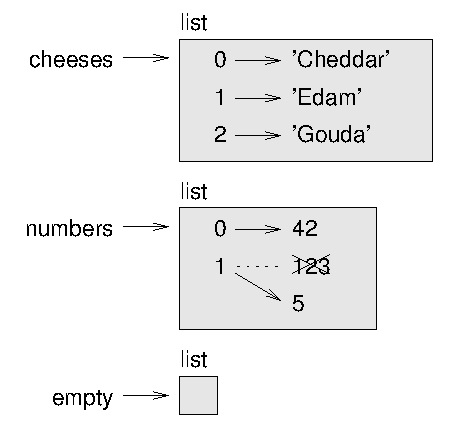
\includegraphics[scale=0.9]{../source/figs/liststate.pdf}}
% \caption{State diagram.}
\caption{状态图。  }
\label{fig.liststate}
\end{figure}

%🍁% Lists are represented by boxes with the word ``list'' outside
%🍁% and the elements of the list inside.  {\tt cheeses} refers to
%🍁% a list with three elements indexed 0, 1 and 2.
%🍁% {\tt numbers} contains two elements; the diagram shows that the
%🍁% value of the second element has been reassigned from 123 to 5.
%🍁% {\tt empty} refers to a list with no elements.
\index{item assignment}  \index{assignment!item}
\index{reassignment}

列表用外部标有 ``list'' 的盒子表示, 盒子内部是列表的元素。  \li{cheeses} 指向一个有3个元素的列表, 3个元素的下标分别是0、1、2。  \li{numbers} 包含两个元素;
状态图显示第二个元素原来是123, 被重新赋值为5。  \li{empty} 对应一个没有元素的列表。

%🍁% List indices work the same way as string indices:

列表下标的工作原理和字符串下标相同:

%🍁% \begin{itemize}
%🍁%
%🍁% \item Any integer expression can be used as an index.
%🍁%
%🍁% \item If you try to read or write an element that does not exist, you
%🍁% get an {\tt IndexError}.
%🍁% \index{exception!IndexError}  \index{IndexError}
%🍁%
%🍁% \item If an index has a negative value, it counts backward from the
%🍁% end of the list.
%🍁%
%🍁% \end{itemize}

\begin{itemize}

\item 任何整数表达式都可以用作下标。

\item 如果你试图读或写一个不存在的元素, 你将会得到一个 {\em 索引错误 \footnote{ \li{IndexError}}}。
\index{exception!IndexError}  \index{IndexError}

\item 如果下标是负数, 它将从列表的末端开始访问列表。

\end{itemize}
\index{list!index}  \index{list!membership}
\index{membership!list}  \index{in operator}
\index{operator!in}

%🍁% The {\tt in} operator also works on lists.

\li{in} 运算符在列表中同样可以使用。

\begin{lstlisting}
>>> cheeses = ['Cheddar', 'Edam', 'Gouda']
>>> 'Edam' in cheeses
True
>>> 'Brie' in cheeses
False
\end{lstlisting}


%🍁% \section{Traversing a list  |  列表遍历}
\section{列表遍历}
\index{list!traversal}  \index{traversal!list}
\index{for loop}  \index{loop!for}
\index{statement!for}
\index{列表!遍历}  \index{遍历!列表}
\index{for 循环}  \index{循环!for}
\index{语句!for}

%🍁% The most common way to traverse the elements of a list is
%🍁% with a {\tt for} loop.  The syntax is the same as for strings:

最常用的遍历列表的方式是使用 \li{for} 循环。  语法和字符串遍历类似:

\begin{lstlisting}
for cheese in cheeses:
    print(cheese)
\end{lstlisting}

%
%🍁% This works well if you only need to read the elements of the
%🍁% list.  But if you want to write or update the elements, you
%🍁% need the indices.  A common way to do that is to combine
%🍁% the built-in functions {\tt range} and {\tt len}:

如果你只需要读取列表中的元素, 这种方法已经足够。  然而, 如果你想要写入或者更新列表中的元素, 你需要通过下标访问。  一种常用的方法是结合内置函数 \li{range} 和 \li{len} :
\index{循环!使用索引}  \index{索引!控制循环}

\begin{lstlisting}
for i in range(len(numbers)):
    numbers[i] = numbers[i] * 2
\end{lstlisting}

%
%🍁% This loop traverses the list and updates each element.  {\tt len}
%🍁% returns the number of elements in the list.  {\tt range} returns
%🍁% a list of indices from 0 to $n-1$, where $n$ is the length of
%🍁% the list.  Each time through the loop {\tt i} gets the index
%🍁% of the next element.  The assignment statement in the body uses
%🍁% {\tt i} to read the old value of the element and to assign the
%🍁% new value.

这个循环将遍历列表并更新每个元素。  \li{len} 返回列表中的元素个数。  \li{range} 返回一个包含从 0 到 $n-1$ 下标的列表, 其中 $n$ 是列表的长度。
每次循环中, \li{i} 得到下一个元素的下标。  循环主体中的赋值语句使用 \li{i} 读取该元素的旧值, 并赋予其一个新值。
\index{item update}  \index{update!item}

%🍁% A {\tt for} loop over an empty list never runs the body:

对一个空列表执行 \li{for} 循环时, 将不会执行循环的主体:

\begin{lstlisting}
for x in []:
    print('This never happens.')
\end{lstlisting}

%
%🍁% Although a list can contain another list, the nested
%🍁% list still counts as a single element.  The length of this list is
%🍁% four:

尽管一个列表可以包含另一个列表, 嵌套的列表本身还是被看作一个单个元素。
下面这个列表的长度是4:
\index{nested list}  \index{list!nested}

\begin{lstlisting}
['spam', 1, ['Brie', 'Roquefort', 'Pol le Veq'], [1, 2, 3]]
\end{lstlisting}


%🍁% \section{List operations  |  列表操作}
\section{列表操作}
\index{list!operation}

%🍁% The {\tt +} operator concatenates lists:

{\em 加号运算符}\li{+} 拼接多个列表:

\index{concatenation!list}  \index{list!concatenation}

\begin{lstlisting}
>>> a = [1, 2, 3]
>>> b = [4, 5, 6]
>>> c = a + b
>>> c
[1, 2, 3, 4, 5, 6]
\end{lstlisting}

%
%🍁% The {\tt *} operator repeats a list a given number of times:

{\em 乘号运算符} \li{*} 以给定次数的重复一个列表:
\index{repetition!list}  \index{list!repetition}

\begin{lstlisting}
>>> [0] * 4
[0, 0, 0, 0]
>>> [1, 2, 3] * 3
[1, 2, 3, 1, 2, 3, 1, 2, 3]
\end{lstlisting}

%
%🍁% The first example repeats {\tt [0]} four times.  The second example
%🍁% repeats the list {\tt [1, 2, 3]} three times.

第一个例子重复 4 次。  第二个例子重复了那个列表 3 次。

%🍁% \section{List slices  |  列表切片}
\section{列表切片}
\index{slice operator}  \index{operator!slice}  \index{index!slice}
\index{list!slice}  \index{slice!list}

%🍁% The slice operator also works on lists:

{\em 切片} (slice) 运算符同样适用于列表:


\begin{lstlisting}
>>> t = ['a', 'b', 'c', 'd', 'e', 'f']
>>> t[1:3]
['b', 'c']
>>> t[:4]
['a', 'b', 'c', 'd']
>>> t[3:]
['d', 'e', 'f']
\end{lstlisting}
%
%🍁% If you omit the first index, the slice starts at the beginning.
%🍁% If you omit the second, the slice goes to the end.  So if you
%🍁% omit both, the slice is a copy of the whole list.

如果你省略第一个索引, 切片将从列表头开始。  如果你省略第二个索引, 切片将会到列表尾结束。
所以如果你两者都省略, 切片就是整个列表的一个拷贝。
\index{list!copy}  \index{slice!copy}
\index{copy!slice}

\begin{lstlisting}
>>> t[:]
['a', 'b', 'c', 'd', 'e', 'f']
\end{lstlisting}

%
%🍁% Since lists are mutable, it is often useful to make a copy
%🍁% before performing operations that modify lists.

由于列表是可变的, 通常在修改列表之前, 对列表进行拷贝是很有用的。
\index{mutability}

%🍁% A slice operator on the left side of an assignment
%🍁% can update multiple elements:

切片运算符放在赋值语句的左边时, 可以一次更新多个元素:
\index{slice!update}  \index{update!slice}

\begin{lstlisting}
>>> t = ['a', 'b', 'c', 'd', 'e', 'f']
>>> t[1:3] = ['x', 'y']
>>> t
['a', 'x', 'y', 'd', 'e', 'f']
\end{lstlisting}

%

% You can add elements to a list by squeezing them into an empty
% slice:

% % \begin{lstlisting}
% >>> t = ['a', 'd', 'e', 'f']
% >>> t[1:1] = ['b', 'c']
% >>> print t
% ['a', 'b', 'c', 'd', 'e', 'f']
% \end{lstlisting}
% \afterverb
%
% And you can remove elements from a list by assigning the empty list to
% them:

% % \begin{lstlisting}
% >>> t = ['a', 'b', 'c', 'd', 'e', 'f']
% >>> t[1:3] = []
% >>> print t
% ['a', 'd', 'e', 'f']
% \end{lstlisting}
% \afterverb
%
% But both of those operations can be expressed more clearly
% with list methods.


%🍁% \section{List methods  |  列表方法}
\section{列表方法}
\index{list!method}
\index{method, list}

%🍁% Python provides methods that operate on lists.  For example,
%🍁% {\tt append} adds a new element to the end of a list:

Python为列表提供了一些方法. 例如, \li{append} 添加一个新元素到列表的末端:

\index{append method}  \index{method!append}

\begin{lstlisting}
>>> t = ['a', 'b', 'c']
>>> t.append('d')
>>> t
['a', 'b', 'c', 'd']
\end{lstlisting}
%
%🍁% {\tt extend} takes a list as an argument and appends all of
%🍁% the elements:

\li{extend} 将接受一个列表作为参数, 并将其其中的所有元素添加至目标列表中:
\index{extend method}  \index{method!extend}

\begin{lstlisting}
>>> t1 = ['a', 'b', 'c']
>>> t2 = ['d', 'e']
>>> t1.extend(t2)
>>> t1
['a', 'b', 'c', 'd', 'e']
\end{lstlisting}

%
%🍁% This example leaves {\tt t2} unmodified.

这个例子中 \li{t2} 没有改动。

%🍁% {\tt sort} arranges the elements of the list from low to high:

\li{sort} 将列表中的元素从小到大进行排序:
\index{sort method}  \index{method!sort}

\begin{lstlisting}
>>> t = ['d', 'c', 'e', 'b', 'a']
>>> t.sort()
>>> t
['a', 'b', 'c', 'd', 'e']
\end{lstlisting}

%
%🍁% Most list methods are void; they modify the list and return {\tt None}.
%🍁% If you accidentally write {\tt t = t.sort()}, you will be disappointed
%🍁% with the result.

大部分的列表方法都是无返回值的;它们对列表进行修改, 然后返回None。
如果你意外的写了 \li{t.sort()}, 你将会对结果感到失望的。
\index{void method}  \index{method!void}
\index{None special value}  \index{special value!None}


%🍁% \section{Map, filter and reduce  |  映射、筛选和归并}
\section{映射、筛选和归并}
\label{filter}

%🍁% To add up all the numbers in a list, you can use a loop like this:

你可以这样使用循环, 对列表中所有元素求和:

% see add.py

\begin{lstlisting}
def add_all(t):
    total = 0
    for x in t:
        total += x
    return total
\end{lstlisting}
%
%🍁% {\tt total} is initialized to 0.  Each time through the loop,
%🍁% {\tt x} gets one element from the list.  The {\tt +=} operator
%🍁% provides a short way to update a variable.  This {\bf augmented assignment %🍁% statement},

\li{total} 被初始化为 0。  每次循环时, \li{x} 从列表中获取一个元素。
运算符 \li{+=} 提供了一个快捷的更新变量的方法。  这个 {\em 增量赋值语句} (augmented assignment statement) 。

\index{update operator}  \index{operator!update}
\index{assignment!augmented}  \index{augmented assignment}

\begin{lstlisting}
    total += x
\end{lstlisting}

%
%🍁% is equivalent to

等价于

\begin{lstlisting}
    total = total + x
\end{lstlisting}

%
%🍁% As the loop runs, {\tt total} accumulates the sum of the
%🍁% elements; a variable used this way is sometimes called an
%🍁% {\bf accumulator}.

当循环执行时, \li{total} 将累计元素的和;一个这样的变量有时被称为 {\em 累加器} (accumulator) 。

\index{accumulator!sum}

%🍁% Adding up the elements of a list is such a common operation
%🍁% that Python provides it as a built-in function, {\tt sum}:

把一个列表中的元素加起来是一个很常用的操作,
所以Python将其设置为一个内建内置函数 \li{sum} :

\begin{lstlisting}
>>> t = [1, 2, 3]
>>> sum(t)
6
\end{lstlisting}
%
%🍁% An operation like this that combines a sequence of elements into
%🍁% a single value is sometimes called {\bf reduce}.

一个像这样的将一系列的元素合并成一个单一值的操作有时称为 {\em 归并} (reduce) 。

\index{reduce pattern}  \index{pattern!reduce}
\index{traversal}

%🍁% Sometimes you want to traverse one list while building
%🍁% another.  For example, the following function takes a list of strings
%🍁% and returns a new list that contains capitalized strings:

有时, 你在构建一个列表时还需要遍历另一个列表。   例如, 下面的函数接受一个字符串列表

\begin{lstlisting}
def capitalize_all(t):
    res = []
    for s in t:
        res.append(s.capitalize())
    return res
\end{lstlisting}

%
%🍁% {\tt res} is initialized with an empty list; each time through
%🍁% the loop, we append the next element.  So {\tt res} is another
%🍁% kind of accumulator.

\li{res} 被初始化为一个空列表;每次循环时, 我们添加下一个元素。
所以 \li{res} 是另一种形式的累加器。

\index{accumulator!list}

%🍁% An operation like \verb"capitalize_all" is sometimes called a {\bf
%🍁% map} because it ``maps'' a function (in this case the method {\tt
%🍁% capitalize}) onto each of the elements in a sequence.

类似 \li{capitalize_all} 这样的操作有时被称为 {\em 映射} (map) , 因为它 ``映射''一个函数(在本例中是方法 \li{capitalize} )到序列中的每个元素上。

\index{map pattern}  \index{pattern!map}
\index{filter pattern}  \index{pattern!filter}

%🍁% Another common operation is to select some of the elements from
%🍁% a list and return a sublist.  For example, the following
%🍁% function takes a list of strings and returns a list that contains
%🍁% only the uppercase strings:

另一个常见的操作是从列表中选择一些元素, 并返回一个子列表。  例如, 下面的函数读取一个字符串列表, 并返回一个仅包含大写字符串的列表:

\begin{lstlisting}
def only_upper(t):
    res = []
    for s in t:
        if s.isupper():
            res.append(s)
    return res
\end{lstlisting}

%
%🍁% {\tt isupper} is a string method that returns {\tt True} if
%🍁% the string contains only upper case letters.

\li{isupper} 是一个字符串方法, 如果字符串仅含有大写字母, 则返回 \li{True}。

%🍁% An operation like \verb"only_upper" is called a {\bf filter} because
%🍁% it selects some of the elements and filters out the others.

类似 \li{only_upper} 这样的操作被称为 {\em 筛选} (filter) , 因为它选中某些元素, 然后剔除剩余的元素。

%🍁% Most common list operations can be expressed as a combination
%🍁% of map, filter and reduce.

大部分常用列表操作可以用映射、筛选和归并这个组合表示。


%🍁% \section{Deleting elements  |  删除元素}
\section{删除元素}
\index{element deletion}  \index{deletion, element of list}

%🍁% There are several ways to delete elements from a list.  If you
%🍁% know the index of the element you want, you can use
%🍁% {\tt pop}:

有多种方法可以从列表中删除一个元素。  如果你知道元素的下标, 你可以使用 \li{pop} :

\index{pop method}  \index{method!pop}

\begin{lstlisting}
>>> t = ['a', 'b', 'c']
>>> x = t.pop(1)
>>> t
['a', 'c']
>>> x
'b'
\end{lstlisting}

%
%🍁% {\tt pop} modifies the list and returns the element that was removed.
%🍁% If you don't provide an index, it deletes and returns the
%🍁% last element.

\li{pop} 修改列表, 并返回被移除的元素。  如果你不提供下标, 它将移除并返回最后一个元素。

%🍁% If you don't need the removed value, you can use the {\tt del}
%🍁% operator:

如果你不需要被移除的元素, 可以使用 \li{del} 运算符:

\index{del operator}  \index{operator!del}

\begin{lstlisting}
>>> t = ['a', 'b', 'c']
>>> del t[1]
>>> t
['a', 'c']
\end{lstlisting}

%
%🍁% If you know the element you want to remove (but not the index), you
%🍁% can use {\tt remove}:

如果你知道要删除的值(但是不知道其下标), 你可以使用 \li{remove} :

\index{remove method}  \index{method!remove}

\begin{lstlisting}
>>> t = ['a', 'b', 'c']
>>> t.remove('b')
>>> t
['a', 'c']
\end{lstlisting}
%
%🍁% The return value from {\tt remove} is {\tt None}.

\li{remove} 的返回值是 \li{None}。

\index{None special value}  \index{special value!None}

%🍁% To remove more than one element, you can use {\tt del} with
%🍁% a slice index:

要移除多个元素, 你可以结合切片索引使用 \li{del} :

\begin{lstlisting}
>>> t = ['a', 'b', 'c', 'd', 'e', 'f']
>>> del t[1:5]
>>> t
['a', 'f']
\end{lstlisting}

%
%🍁% As usual, the slice selects all the elements up to but not
%🍁% including the second index.

同样的, 切片选择到第二个下标(不包含第二个下标)处的所有元素。


%🍁% \section{Lists and strings  |  列表和字符串}
\section{列表和字符串}
\index{list}  \index{string}
\index{sequence}

%🍁% A string is a sequence of characters and a list is a sequence
%🍁% of values, but a list of characters is not the same as a
%🍁% string.  To convert from a string to a list of characters,
%🍁% you can use {\tt list}:

一个字符串是多个字符组成的序列, 一个列表是多个值组成的序列。  但是一个由字符组成的列表不同于字符串。  可以使用 \li{list} 将一个字符串转换为字符的列表:

\index{list!function}  \index{function!list}

\begin{lstlisting}
>>> s = 'spam'
>>> t = list(s)
>>> t
['s', 'p', 'a', 'm']
\end{lstlisting}

%
%🍁% Because {\tt list} is the name of a built-in function, you should
%🍁% avoid using it as a variable name.  I also avoid {\tt l} because
%🍁% it looks too much like {\tt 1}.  So that's why I use {\tt t}.

由于 \li{list} 是内置函数的名称, 你应避免将它用作变量名。  我同样避免使用 \li{l} , 因为它看起来很像 \li{1}。  这就是为什么我用了 \li{t} 。

%🍁% The {\tt list} function breaks a string into individual letters.  If
%🍁% you want to break a string into words, you can use the {\tt split}
%🍁% method:

\li{list} 函数将字符串分割成单独的字符。  如果你想将一个字符串分割成一些单词, 你可以使用 \li{split} 方法:

\index{split method}  \index{method!split}

\begin{lstlisting}
>>> s = 'pining for the fjords'
>>> t = s.split()
>>> t
['pining', 'for', 'the', 'fjords']
\end{lstlisting}

%
%🍁% An optional argument called a {\bf delimiter} specifies which
%🍁% characters to use as word boundaries.
%🍁% The following example
%🍁% uses a hyphen as a delimiter:

可以提高一个叫做 {\em 分隔符} (delimiter) 的可选参数, 指定什么字符作为单词之间的分界线。  下面的例子使用连字符作为分隔符:

\index{optional argument}  \index{argument!optional}
\index{delimiter}

\begin{lstlisting}
>>> s = 'spam-spam-spam'
>>> delimiter = '-'
>>> t = s.split(delimiter)
>>> t
['spam', 'spam', 'spam']
\end{lstlisting}

%
%🍁% {\tt join} is the inverse of {\tt split}.  It
%🍁% takes a list of strings and
%🍁% concatenates the elements.  {\tt join} is a string method,
%🍁% so you have to invoke it on the delimiter and pass the
%🍁% list as a parameter:

\li{join} 的功能和 \li{split} 相反。  它将一个字符串列表的元素拼接起来。  \li{join} 是一个字符串方法, 所以你需要在一个分隔符上调用它, 并传入一个列表作为参数:

\index{join method}  \index{method!join}
\index{concatenation}

\begin{lstlisting}
>>> t = ['pining', 'for', 'the', 'fjords']
>>> delimiter = ' '
>>> s = delimiter.join(t)
>>> s
'pining for the fjords'
\end{lstlisting}

%
%🍁% In this case the delimiter is a space character, so
%🍁% {\tt join} puts a space between words.  To concatenate
%🍁% strings without spaces, you can use the empty string,
%🍁% \verb"''", as a delimiter.

在这个例子中, 分隔符是一个空格, 所以 \li{join} 在单词之间添加一个空格。  如果不使用空格拼接字符串, 你可以使用空字符串 \li{''} 作为分隔符。

\index{empty string}  \index{string!empty}


%🍁% \section{Objects and values  |  对象和值}
\section{对象和值}
\label{equivalence}
\index{object}  \index{value}

%🍁% If we run these assignment statements:

如果我们执行下面的赋值语句:

\begin{lstlisting}
a = 'banana'
b = 'banana'
\end{lstlisting}

%
%🍁% We know that {\tt a} and {\tt b} both refer to a
%🍁% string, but we don't
%🍁% know whether they refer to the {\em same} string.
%🍁% There are two possible states, shown in Figure~\ref{fig.list1}.

我们知道 \li{a} 和 \li{b} 都指向一个字符串, 但是我们不知道是否他们指向 {\bf 同一个} 字符串。  这里有两种可能的状态, 如 图~\ref{fig.list1} 所示。

\index{aliasing}

\begin{figure}
\centerline
{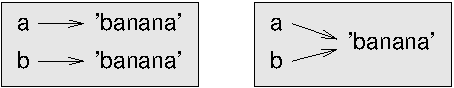
\includegraphics[scale=0.8]{../source/figs/list1.pdf}}
\caption{状态图。}
\label{fig.list1}
\end{figure}

%🍁% In one case, {\tt a} and {\tt b} refer to two different objects that
%🍁% have the same value.  In the second case, they refer to the same
%🍁% object.

一种情况是, \li{a} 和 \li{b} 指向两个有相同值的不同对象。
第二种情况是, 它们指向同一个对象。

\index{is operator}  \index{operator!is}

%🍁% To check whether two variables refer to the same object, you can
%🍁% use the {\tt is} operator.

为了查看两个变量是否指向同一个对象, 你可以使用 \li{is} 运算符。

\begin{lstlisting}
>>> a = 'banana'
>>> b = 'banana'
>>> a is b
True
\end{lstlisting}

%
%🍁% In this example, Python only created one string object, and both {\tt
%🍁%   a} and {\tt b} refer to it.  But when you create two lists, you get
%🍁% two objects:

在这个例子中, Python仅生成了一个字符串对象, \li{a} 和 \li{b} 都指向它。  但是当你创建两个列表时, 你得到的是两个对象:

\begin{lstlisting}
>>> a = [1, 2, 3]
>>> b = [1, 2, 3]
>>> a is b
False
\end{lstlisting}

%
%🍁% So the state diagram looks like Figure~\ref{fig.list2}.

所以状态图如图~\ref{fig.list2}所示。

\index{state diagram}  \index{diagram!state}

\begin{figure}
\centerline
{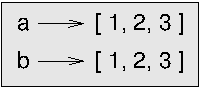
\includegraphics[scale=0.8]{../source/figs/list2.pdf}}
\caption{状态图。}
\label{fig.list2}
\end{figure}

%🍁% In this case we would say that the two lists are {\bf equivalent},
%🍁% because they have the same elements, but not {\bf identical}, because
%🍁% they are not the same object.  If two objects are identical, they are
%🍁% also equivalent, but if they are equivalent, they are not necessarily
%🍁% identical.

在这个例子中, 我们称这两个列表是 {\bf 相等\footnote{equivalent}}的, 因为它们有相同的元素。  但它们并不 {\bf 相同\footnote{identical}} , 因为他们不是同一个对象。  如果两个对象 {\bf 相同}, 它们也是相等的, 但是如果它们是相等的, 它们不一定是相同的。

\index{equivalence}  \index{identity}

%🍁% Until now, we have been using ``object'' and ``value''
%🍁% interchangeably, but it is more precise to say that an object has a
%🍁% value.  If you evaluate {\tt [1, 2, 3]}, you get a list
%🍁% object whose value is a sequence of integers.  If another
%🍁% list has the same elements, we say it has the same value, but
%🍁% it is not the same object.

至此, 我们一直在等价地使用``对象'' 和 ``值'', 但是更准确的说, 一个对象拥有一个值。  如果你对 \li{[1, 2, 3]} 求值, 会得到一个值为整数序列的列表对象。
如果另一个列表有同样的元素, 我们说它们有相同的值, 但是它们并不是同一个对象。

\index{object}  \index{value}


%🍁% \section{Aliasing  |  别名}
\section{别名}
\index{aliasing}  \index{reference!aliasing}

%🍁% If {\tt a} refers to an object and you assign {\tt b = a},
%🍁% then both variables refer to the same object:

如果 \li{a} 指向一个对象, 然后你赋值 \li{b = a} , 那么两个变量指向同一个对象:

\begin{lstlisting}
>>> a = [1, 2, 3]
>>> b = a
>>> b is a
True
\end{lstlisting}

%
%🍁% The state diagram looks like Figure~\ref{fig.list3}.

状态图如图~\ref{fig.list3} 所示。

\index{state diagram}  \index{diagram!state}

\begin{figure}
\centerline
{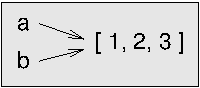
\includegraphics[scale=0.8]{../source/figs/list3.pdf}}
\caption{状态图。}
\label{fig.list3}
\end{figure}

%🍁% The association of a variable with an object is called a {\bf
%🍁% reference}.  In this example, there are two references to the same
%🍁% object.

变量和对象之间的关联称为 {\em 引用} (reference) 。
在这个例子中, 有两个对同一个对象的引用。

\index{reference}

%🍁% An object with more than one reference has more
%🍁% than one name, so we say that the object is {\bf aliased}.

如果一个对象有多于一个引用, 那它也会有多个名称,
我们称这个对象是 {\bf 有别名\footnote{aliased; 别名, alias。}的} 。

\index{mutability}

%🍁% If the aliased object is mutable, changes made with one alias affect
%🍁% the other:

如果一个有别名的对象是可变的, 对其中一个别名的改变对影响到其它的别名:

\begin{lstlisting}
>>> b[0] = 42
>>> a
[42, 2, 3]
\end{lstlisting}

%
%🍁% Although this behavior can be useful, it is error-prone.  In general,
%🍁% it is safer to avoid aliasing when you are working with mutable
%🍁% objects.

尽管这个行为很有用, 但是容易导致出现错误。
通常, 避免对于可变对象使用别名相对更安全。

\index{immutability}

%🍁% For immutable objects like strings, aliasing is not as much of a
%🍁% problem.  In this example:

对于像字符串这样的不可变对象, 使用别名没有什么问题。  例如:

\begin{lstlisting}
a = 'banana'
b = 'banana'
\end{lstlisting}

%
%🍁% It almost never makes a difference whether {\tt a} and {\tt b} refer
%🍁% to the same string or not.

\li{a} 和 \li{b} 是否指向同一个字符串基本上没有什么影响。


%🍁% \section{List arguments  |  列表参数}
\section{列表参数}
\label{list.arguments}
\index{list!as argument}  \index{argument}
\index{argument!list}  \index{reference}
\index{parameter}

\index{列表!参数}  \index{实参}
\index{参数!列表}  \index{引用}
\index{参数}

%🍁% When you pass a list to a function, the function gets a reference to
%🍁% the list.  If the function modifies the list, the caller sees
%🍁% the change.  For example, \verb"delete_head" removes the first element
%🍁% from a list:

当你将一个列表作为参数传给一个函数, 函数将得到这个列表的一个引用。  如果函数对这个列表进行了修改, 会在调用者中有所体现。  例如, ``delete\_head'' 删除列表的第一个元素:

\begin{lstlisting}
def delete_head(t):
    del t[0]
\end{lstlisting}

%
%🍁% Here's how it is used:

这样使用这个函数:

\begin{lstlisting}
>>> letters = ['a', 'b', 'c']
>>> delete_head(letters)
>>> letters
['b', 'c']
\end{lstlisting}

%
%🍁% The parameter {\tt t} and the variable {\tt letters} are
%🍁% aliases for the same object.  The stack diagram looks like
%🍁% Figure~\ref{fig.stack5}.

参数 \li{t} 和变量 \li{letters} 是同一个对象的别名。
其堆栈图如图~\ref{fig.stack5}所示。

\index{stack diagram}  \index{diagram!stack}

\begin{figure}
\centerline
{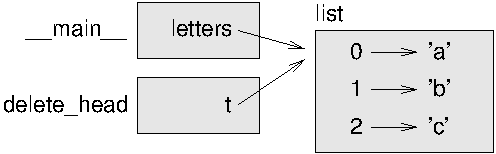
\includegraphics[scale=0.8]{../source/figs/stack5.pdf}}
\caption{Stack diagram.}
\label{fig.stack5}
\end{figure}

%🍁% Since the list is shared by two frames, I drew
%🍁% it between them.

由于列表被两个帧共享, 我把它画在它们中间。

%🍁% It is important to distinguish between operations that
%🍁% modify lists and operations that create new lists.  For
%🍁% example, the {\tt append} method modifies a list, but the
%🍁% {\tt +} operator creates a new list:

需要注意的是修改列表操作和创建列表操作间的区别。
例如, \li{append} 方法是修改一个列表, 而 \li{+} 运算符是创建一个新的列表:

\index{append method}  \index{method!append}
\index{list!concatenation}  \index{concatenation!list}

%
\begin{lstlisting}
>>> t1 = [1, 2]
>>> t2 = t1.append(3)
>>> t1
[1, 2, 3]
>>> t2
None
\end{lstlisting}

%
%🍁% {\tt append} modifies the list and returns {\tt None}.

\li{append} 修改列表并返回 \li{None}。

%
\begin{lstlisting}
>>> t3 = t1 + [4]
>>> t1
[1, 2, 3]
>>> t3
[1, 2, 3, 4]
>>> t1
\end{lstlisting}

%
%🍁% The {\tt +} operator creates a new list and leaves the
%🍁% original list unchanged.

运算符 \li{+} 创建了一个新列表, 而不改变原始的列表。

%🍁% This difference is important when you write functions that
%🍁% are supposed to modify lists.  For example, this function
%🍁% {\em does not} delete the head of a list:

如果你要编写一个修改列表的函数, 这一点就很重要。
例如, 这个函数 {\em 不会} 删除列表的第一个元素:

%
\begin{lstlisting}
def bad_delete_head(t):
    t = t[1:]              # WRONG!
\end{lstlisting}

%
%🍁% The slice operator creates a new list and the assignment
%🍁% makes {\tt t} refer to it, but that doesn't affect the caller.

切片运算符创建了一个新列表, 然后这个表达式让 \li{t} 指向了它,
但是并不会影响原来被调用的列表。

\index{slice operator}  \index{operator!slice}

%
\begin{lstlisting}
>>> t4 = [1, 2, 3]
>>> bad_delete_head(t4)
>>> t4
[1, 2, 3]
\end{lstlisting}

%
%🍁% At the beginning of \verb"bad_delete_head", {\tt t} and {\tt t4}
%🍁% refer to the same list.  At the end, {\tt t} refers to a new list,
%🍁% but {\tt t4} still refers to the original, unmodified list.

在 \li{bad_delete_head} 的开始处, \li{t} 和 \li{t4} 指向同一个列表。  在结束时, \li{t} 指向一个新列表, 但是 \li{t4} 仍然指向原来的、没有被改动的列表。

%🍁% An alternative is to write a function that creates and
%🍁% returns a new list.  For example, {\tt tail} returns all but the first
%🍁% element of a list:

一个替代的写法是, 写一个创建并返回一个新列表的函数。
例如, \li{tail} 返回列表中除了第一个之外的所有元素:

\begin{lstlisting}
def tail(t):
    return t[1:]
\end{lstlisting}

%
%🍁% This function leaves the original list unmodified.
%🍁% Here's how it is used:

这个函数不会修改原来的列表。  下面是函数的使用方法:

\begin{lstlisting}
>>> letters = ['a', 'b', 'c']
>>> rest = tail(letters)
>>> rest
['b', 'c']
\end{lstlisting}


%🍁% \section{Debugging  |  调试}
\section{调试}
\index{debugging}

%🍁% Careless use of lists (and other mutable objects)
%🍁% can lead to long hours of debugging.  Here are some common
%🍁% pitfalls and ways to avoid them:

粗心地使用列表(以及其他可变对象)会导致长时间的调试。
下面列举一些常见的陷阱以及避免它们的方法:

%🍁% \begin{enumerate}
%🍁%
%🍁% \item Most list methods modify the argument and
%🍁%   return {\tt None}.  This is the opposite of the string methods,
%🍁%   which return a new string and leave the original alone.
%🍁%
%🍁% If you are used to writing string code like this:
%🍁%
%🍁% \begin{lstlisting}
%🍁% word = word.strip()
%🍁% \end{lstlisting}
%🍁%
%🍁% It is tempting to write list code like this:
%🍁%
%🍁% \begin{lstlisting}
%🍁% t = t.sort()           # WRONG!
%🍁% \end{lstlisting}
%🍁% \index{sort method}
%🍁% \index{method!sort}
%🍁%
%🍁% Because {\tt sort} returns {\tt None}, the
%🍁% next operation you perform with {\tt t} is likely to fail.
%🍁%
%🍁% Before using list methods and operators, you should read the
%🍁% documentation carefully and then test them in interactive mode.
%🍁%
%🍁% \item Pick an idiom and stick with it.
%🍁%
%🍁% Part of the problem with lists is that there are too many
%🍁% ways to do things.  For example, to remove an element from
%🍁% a list, you can use {\tt pop}, {\tt remove}, {\tt del},
%🍁% or even a slice assignment.
%🍁%
%🍁% To add an element, you can use the {\tt append} method or
%🍁% the {\tt +} operator.  Assuming that {\tt t} is a list and
%🍁% {\tt x} is a list element, these are correct:
%🍁%
%🍁% \begin{lstlisting}
%🍁% t.append(x)
%🍁% t = t + [x]
%🍁% t += [x]
%🍁% \end{lstlisting}
%🍁%
%🍁% And these are wrong:
%🍁%
%🍁% \begin{lstlisting}
%🍁% t.append([x])          # WRONG!
%🍁% t = t.append(x)        # WRONG!
%🍁% t + [x]                # WRONG!
%🍁% t = t + x              # WRONG!
%🍁% \end{lstlisting}
%🍁%
%🍁% Try out each of these examples in interactive mode to make sure
%🍁% you understand what they do.  Notice that only the last
%🍁% one causes a runtime error; the other three are legal, but they
%🍁% do the wrong thing.
%🍁%
%🍁%
%🍁% \item Make copies to avoid aliasing.
%🍁% \index{aliasing!copying to avoid}
%🍁% \index{copy!to avoid aliasing}
%🍁%
%🍁% If you want to use a method like {\tt sort} that modifies
%🍁% the argument, but you need to keep the original list as
%🍁% well, you can make a copy.
%🍁%
%🍁% \begin{lstlisting}
%🍁% >>> t = [3, 1, 2]
%🍁% >>> t2 = t[:]
%🍁% >>> t2.sort()
%🍁% >>> t
%🍁% [3, 1, 2]
%🍁% >>> t2
%🍁% [1, 2, 3]
%🍁% \end{lstlisting}
%🍁%
%🍁% In this example you could also use the built-in function {\tt sorted},
%🍁% which returns a new, sorted list and leaves the original alone.
%🍁%
%🍁% \begin{lstlisting}
%🍁% >>> t2 = sorted(t)
%🍁% >>> t
%🍁% [3, 1, 2]
%🍁% >>> t2
%🍁% [1, 2, 3]
%🍁% \end{lstlisting}
%🍁%
%🍁% \end{enumerate}


\begin{enumerate}

\item 大多数的列表方法会对参数进行修改, 然后返回 \li{None} 。  这和字符串方法相反, 后者保留原始的字符串并返回一个新的字符串。

如果你习惯这样写字符串代码:

\begin{lstlisting}
word = word.strip()
\end{lstlisting}

那么你很可能会写出下面的列表代码:

\begin{lstlisting}
t = t.sort()           # WRONG!
\end{lstlisting}
\index{sort method}
\index{method!sort}

因为 \li{sort} 返回 \li{None} , 所以你的下一个对 \li{t} 执行的操作很可能会失败。

在使用 \li{list} 方法和操作符之前, 你应该仔细阅读文档, 然后在交互模式下测试。

\item 选择一种写法, 坚持下去。

列表的一个问题就是有太多方法可以做同样的事情。   例如, 要删除列表中的一个元素, 你可以使用 \li{pop} 、 \li{remove} 、 \li{del} 甚至是切片赋值。

 要添加一个元素, 你可以使用 \li{append} 方法或者 \li{+} 运算符。  假设 \li{t} 是一个列表, \li{x} 是一个列表元素, 以下这些写法都是正确的:

\begin{lstlisting}
t.append(x)
t = t + [x]
t += [x]
\end{lstlisting}

而这些是错误的:

\begin{lstlisting}
t.append([x])          # WRONG!
t = t.append(x)        # WRONG!
t + [x]                # WRONG!
t = t + x              # WRONG!
\end{lstlisting}

在交互模式下尝试每一个例子, 保证你明白它们做了什么。   注意只有最后一个会导致运行时错误;其他的都是合乎规范的的, 但结果却是错的。


\item 通过创建拷贝来避免别名.
\index{aliasing!copying to avoid}  \index{copy!to avoid aliasing}

如果你要使用类似 \li{sort} 这样的方法来修改参数,
   但同时有要保留原列表, 你可以创建一个拷贝。


\begin{lstlisting}
>>> t = [3, 1, 2]
>>> t2 = t[:]
>>> t2.sort()
>>> t
[3, 1, 2]
>>> t2
[1, 2, 3]
\end{lstlisting}

在这个例子中, 你还可以使用内置函数 \li{sorted}, 它将返回一个新的已排序的列表, 原列表将保持不变。

\begin{lstlisting}
>>> t2 = sorted(t)
>>> t
[3, 1, 2]
>>> t2
[1, 2, 3]
\end{lstlisting}

\end{enumerate}


%🍁% \section{Glossary  |  术语表}
\section{术语表}

\begin{description}

%🍁% \item[list:] A sequence of values.
%🍁% \index{list}

\item[列表 (list):] 多个值组成的序列。
\index{list}

%🍁% \item[element:] One of the values in a list (or other sequence),
%🍁% also called items.
%🍁% \index{element}

\item[元素 (element):] 列表(或序列)中的一个值, 也称为项。
\index{element}

%🍁% \item[nested list:] A list that is an element of another list.
%🍁% \index{nested list}

\item[嵌套列表 (nested list):] 作为另一个列表的元素的列表。
\index{nested list}

%🍁% \item[accumulator:] A variable used in a loop to add up or
%🍁% accumulate a result.
%🍁% \index{accumulator}

\item[累加器 (accumulator):] 循环中用于相加或累积出一个结果的变量。
\index{accumulator}

%🍁% \item[augmented assignment:] A statement that updates the value
%🍁% of a variable using an operator like \verb"+=".
%🍁% \index{assignment!augmented}  \index{augmented assignment}
%🍁% \index{traversal}

\item[增量赋值语句 (augmented assignment):] 一个使用类似 \li{+=} 操作符来更新一个变量的值的语句。
\index{assignment!augmented}  \index{augmented assignment}
\index{traversal}

%🍁% \item[reduce:] A processing pattern that traverses a sequence
%🍁% and accumulates the elements into a single result.
%🍁% \index{reduce pattern}  \index{pattern!reduce}

\item[归并 (reduce):] 遍历序列, 将所有元素求和为一个值的处理模式。
\index{reduce pattern}  \index{pattern!reduce}

%🍁% \item[map:] A processing pattern that traverses a sequence and
%🍁% performs an operation on each element.
%🍁% \index{map pattern}  \index{pattern!map}

\item[映射 (map):] 遍历序列, 对每个元素执行操作的处理模式。
\index{map pattern}  \index{pattern!map}

%🍁% \item[filter:] A processing pattern that traverses a list and
%🍁% selects the elements that satisfy some criterion.
%🍁% \index{filter pattern}  \index{pattern!filter}

\item[筛选 (filter):] 遍历序列, 选出满足一定标准的元素的处理模式。
\index{filter pattern}  \index{pattern!filter}

%🍁% \item[object:] Something a variable can refer to.  An object
%🍁% has a type and a value.
%🍁% \index{object}

\item[对象 (object)] 变量可以指向的东西。  一个对象有数据类型和值。
\index{object}

%🍁% \item[equivalent:] Having the same value.
%🍁% \index{equivalent}

\item[相等 (equivalent):] 有相同的值。
\index{equivalent}

%🍁% \item[identical:] Being the same object (which implies equivalence).
%🍁% \index{identical}

\item[相同 (identical):] 是同一个对象(隐含着相等)。
\index{identical}

%🍁% \item[reference:] The association between a variable and its value.
%🍁% \index{reference}

\item[引用 (reference):] 一个变量和它的值之间的关联。
\index{reference}

%🍁% \item[aliasing:] A circumstance where two or more variables refer to the same
%🍁% object.
%🍁% \index{aliasing}

\item[别名使用:] 两个或者两个以上变量指向同一个对象的情况。
\index{aliasing}

%🍁% \item[delimiter:] A character or string used to indicate where a
%🍁% string should be split.
%🍁% \index{delimiter}

\item[分隔符 (delimiter):] 一个用于指示字符串分割位置的字符或者字符串。
\index{delimiter}

\end{description}


%🍁% \section{Exercises  |  练习}
\section{练习}

%🍁% You can download solutions to these exercises from
%🍁% \url{http://thinkpython2.com/code/list_exercises.py}.

你可以从 \href{http://thinkpython2.com/code/list_exercises.py}{此处} 下载这些练习的答案。

\begin{exercise}

%🍁% Write a function called \verb"nested_sum" that takes a list of lists
%🍁% of integers and adds up the elements from all of the nested lists.
%🍁% For example:

编写一个叫做 {\em \li{nested_sum}} 的函数, 接受一个由一些整数列表构成的列表作为参数, 并将所有嵌套列表中的元素相加。  例如:

\begin{em}
\begin{lstlisting}
>>> t = [[1, 2], [3], [4, 5, 6]]
>>> nested_sum(t)
21
\end{lstlisting}
\end{em}

\end{exercise}

\begin{exercise}
\label{cumulative}
\index{cumulative sum}

%🍁% Write a function called {\tt cumsum} that takes a list of numbers and
%🍁% returns the cumulative sum; that is, a new list where the $i$th
%🍁% element is the sum of the first $i+1$ elements from the original list.
%🍁% For example:

编写一个叫做 {\em \li{cumsum}} 的函数, 接受一个由数值组成的列表, 并返回累加和;
即一个新列表, 其中第 $i+1$ 个元素是原列表中前 $i$ 个元素的和。
例如:

\begin{em}
\begin{lstlisting}
>>> t = [1, 2, 3]
>>> cumsum(t)
[1, 3, 6]
\end{lstlisting}
\end{em}

\end{exercise}

\begin{exercise}

%🍁% Write a function called \verb"middle" that takes a list and
%🍁% returns a new list that contains all but the first and last
%🍁% elements.  For example:

编写一个叫做 {\em \li{middle}} 的函数, 接受一个列表作为参数, 并返回一个除了第一个和最后一个元素的列表。
例如:

\begin{em}
\begin{lstlisting}
>>> t = [1, 2, 3, 4]
>>> middle(t)
[2, 3]
\end{lstlisting}
\end{em}

\end{exercise}

\begin{exercise}

%🍁% Write a function called \verb"chop" that takes a list, modifies it
%🍁% by removing the first and last elements, and returns {\tt None}.
%🍁% For example:

编写一个叫做 {\em \li{chop}} 的函数, 接受一个列表作为参数, 移除第一个和最后一个元素, 并返回 {\em \li{None}}。
例如:

\begin{em}
\begin{lstlisting}
>>> t = [1, 2, 3, 4]
>>> chop(t)
>>> t
[2, 3]
\end{lstlisting}
\end{em}

\end{exercise}


\begin{exercise}
%🍁% Write a function called \verb"is_sorted" that takes a list as a
%🍁% parameter and returns {\tt True} if the list is sorted in ascending
%🍁% order and {\tt False} otherwise.  For example:

编写一个叫做 {\em \li{is_sorted}} 的函数, 接受一个列表作为参数,
如果列表是递增排列的则返回 {\em \li{True}} , 否则返回 {\em \li{False}}。
例如:

\begin{em}
\begin{lstlisting}
>>> is_sorted([1, 2, 2])
True
>>> is_sorted(['b', 'a'])
False
\end{lstlisting}
\end{em}

\end{exercise}


\begin{exercise}
\label{anagram}
\index{anagram}

%🍁% Two words are anagrams if you can rearrange the letters from one
%🍁% to spell the other.  Write a function called \verb"is_anagram"
%🍁% that takes two strings and returns {\tt True} if they are anagrams.


如果可以通过重排一个单词中字母的顺序, 得到另外一个单词, 那么称这两个单词是变位词。
编写一个叫做 {\em \li{is_anagram}} 的函数, 接受两个字符串作为参数,
如果它们是变位词则返回 {\em \li{True}} 。
\end{exercise}



\begin{exercise}
\label{duplicate}
\index{duplicate}  \index{uniqueness}

%🍁% Write a function called \verb"has_duplicates" that takes
%🍁% a list and returns {\tt True} if there is any element that
%🍁% appears more than once.  It should not modify the original
%🍁% list.

编写一个叫做 {\em \li{has_duplicates}} 的函数, 接受一个列表作为参数,
如果一个元素在列表中出现了不止一次, 则返回 {\em \li{True}} 。
这个函数不能改变原列表。

\end{exercise}


\begin{exercise}

%🍁% This exercise pertains to the so-called Birthday Paradox, which you
%🍁% can read about at \url{http://en.wikipedia.org/wiki/Birthday_paradox}.
\index{birthday paradox}

这个习题与所谓的生日悖论有关。
你可以在 \href{http://en.wikipedia.org/wiki/Birthday_paradox}{维基百科}了解更多相关的内容。
\index{维基百科}

%🍁% If there are 23 students in your class, what are the chances
%🍁% that two of you have the same birthday?  You can estimate this
%🍁% probability by generating random samples of 23 birthdays
%🍁% and checking for matches.  Hint: you can generate random birthdays
%🍁% with the {\tt randint} function in the {\tt random} module.

如果你的班级上有 {\em 23} 个学生, {\em 2} 个学生生日相同的概率是多少?
你可以通过随机产生 {\em 23} 个生日, 并检查匹配来估算概率。
提示:你可以使用 {\em \li{random}} 模块中的 {\em \li{randint}} 函
数来生成随机生日。

\index{random module}  \index{module!random}
\index{randint function}  \index{function!randint}

%🍁% You can download my
%🍁% solution from \url{http://thinkpython2.com/code/birthday.py}.

你可以参考 \href{http://thinkpython2.com/code/birthday.py}{我的答案}。

\end{exercise}



\begin{exercise}
\index{append method}  \index{method append}
\index{list!concatenation}  \index{concatenation!list}

%🍁% Write a function that reads the file {\tt words.txt} and builds
%🍁% a list with one element per word.  Write two versions of
%🍁% this function, one using the {\tt append} method and the
%🍁% other using the idiom {\tt t = t + [x]}.  Which one takes
%🍁% longer to run?  Why?

编写一个函数, 读取文件 {\em \li{words.txt}}, 建立一个列表, 其中每个单词为一个元素。
编写两个版本, 一个使用 {\em \li{append}} 方法, 另一个使用 {\em \li{t = t + [x]}}。
那个版本运行得慢?为什么?

%🍁% Solution: \url{http://thinkpython2.com/code/wordlist.py}.

\href{http://thinkpython2.com/code/wordlist.py}{参考答案}

\index{time module}  \index{module!time}

\end{exercise}


\begin{exercise}
\label{wordlist1}
\label{bisection}
\index{membership!bisection search}  \index{bisection search}
\index{search, bisection}  \index{membership!binary search}
\index{binary search}  \index{search, binary}

\index{membership!bisection search}  \index{bisection search}
\index{search, bisection}  \index{membership!binary search}
\index{二叉树搜索}  \index{搜索, 二叉树}


%🍁% To check whether a word is in the word list, you could use
%🍁% the {\tt in} operator, but it would be slow because it searches
%🍁% through the words in order.

使用 {\em \li{in}} 运算符可以检查一个单词是否在单词表中, 但这很慢, 因为它是按顺序查找单词。

%🍁% Because the words are in alphabetical order, we can speed things up
%🍁% with a bisection search (also known as binary search), which is
%🍁% similar to what you do when you look a word up in the dictionary.  You
%🍁% start in the middle and check to see whether the word you are looking
%🍁% for comes before the word in the middle of the list.  If so, you
%🍁% search the first half of the list the same way.  Otherwise you search
%🍁% the second half.

由于单词是按照字母顺序排序的, 我们可以使用两分法{\em (}也称二叉树搜索{\em)}来加快速度,
类似于在字典中查找单词的方法。  你从中间开始, 如果你要找的单词在中间的单词之前, 你查找前半部分, 否则你查找后半部分。

%🍁% Either way, you cut the remaining search space in half.  If the
%🍁% word list has 113,809 words, it will take about 17 steps to
%🍁% find the word or conclude that it's not there.

不管怎样, 你都会将搜索范围减小一半。
如果单词表有 {\em 113,809} 个单词, 你只需要 {\em 17} 步就可以找到这个单词, 或着得出单词不存在的结论。

%🍁% Write a function called \verb"in_bisect" that takes a sorted list
%🍁% and a target value and returns the index of the value
%🍁% in the list if it's there, or {\tt None} if it's not.

编写一个叫做 {\em \li{in_bisect}} 的函数, 接受一个已排序的列表和一个目标值作为参数,
返回该值在列表中的位置, 如果不存在则返回 {\em \li{None}} 。

\index{bisect module}  \index{module!bisect}

%🍁% Or you could read the documentation of the {\tt bisect} module
%🍁% and use that!  Solution: \url{http://thinkpython2.com/code/inlist.py}.

或者你可以阅读 {\em \li{bisect}} 模块的文档并使用它!

\href{http://thinkpython2.com/code/inlist.py}{参考答案}

\end{exercise}

\begin{exercise}
\index{reverse word pair}

%🍁% Two words are a ``reverse pair'' if each is the reverse of the
%🍁% other.  Write a program that finds all the reverse pairs in the
%🍁% word list.  Solution: \url{http://thinkpython2.com/code/reverse_pair.py}.

两个单词中如果一个是另一个的反转, 则二者被称为是``反转词对''。
编写一个函数, 找出单词表中所有的反转词对。

\href{http://thinkpython2.com/code/reverse_pair.py}{参考答案}

\end{exercise}

\begin{exercise}
\index{interlocking words}

%🍁% Two words ``interlock'' if taking alternating letters from each forms
%🍁% a new word.  For example, ``shoe'' and ``cold''
%🍁% interlock to form ``schooled''.
%🍁% Solution: \url{http://thinkpython2.com/code/interlock.py}.
%🍁% Credit: This exercise is inspired by an example at \url{http://puzzlers.org}.

如果交替的从两个单词中取出字符将组成一个新的单词, 这两个单词被称为是``连锁词''。
例如, {\em ``shoe''} 和 {\em ``cold''} 连锁后成为 {\em ``schooled''}。

\begin{enumerate}

%🍁% \item Write a program that finds all pairs of words that interlock.
%🍁%   Hint: don't enumerate all pairs!

\item 编写一个程序, 找出单词表中所有的连锁词。  提示:不要枚举所有的单词对。

%🍁% \item Can you find any words that are three-way interlocked; that is,
%🍁%   every third letter forms a word, starting from the first, second or
%🍁%   third?

\item 你能够找到三重连锁的单词吗?即每个字母依次从3个单词得到。

\end{enumerate}
\end{exercise}



\chapter{Dictionaries}

This chapter presents another built-in type called a dictionary.
Dictionaries are one of Python's best features; they are the
building blocks of many efficient and elegant algorithms.


\section{A dictionary is a mapping}

\index{dictionary}
\index{dictionary}
\index{type!dict}
\index{key}
\index{key-value pair}
\index{index}
A {\bf dictionary} is like a list, but more general.  In a list,
the indices have to be integers; in a dictionary they can
be (almost) any type.

A dictionary contains a collection of indices, which are called {\bf
  keys}, and a collection of values.  Each key is associated with a
single value.  The association of a key and a value is called a {\bf
  key-value pair} or sometimes an {\bf item}.  \index{item}

In mathematical language, a dictionary represents a {\bf mapping}
from keys to values, so you can also say that each key
``maps to'' a value.
As an example, we'll build a dictionary that maps from English
to Spanish words, so the keys and the values are all strings.

The function {\tt dict} creates a new dictionary with no items.
Because {\tt dict} is the name of a built-in function, you
should avoid using it as a variable name.
\index{dict function}
\index{function!dict}

\begin{verbatim}
>>> eng2sp = dict()
>>> eng2sp
{}
\end{verbatim}

The squiggly-brackets, \verb"{}", represent an empty dictionary.
To add items to the dictionary, you can use square brackets:
\index{squiggly bracket}
\index{bracket!squiggly}

\begin{verbatim}
>>> eng2sp['one'] = 'uno'
\end{verbatim}
%
This line creates an item that maps from the key
\verb"'one'" to the value \verb"'uno'".  If we print the
dictionary again, we see a key-value pair with a colon
between the key and value:

\begin{verbatim}
>>> eng2sp
{'one': 'uno'}
\end{verbatim}
%
This output format is also an input format.  For example,
you can create a new dictionary with three items:

\begin{verbatim}
>>> eng2sp = {'one': 'uno', 'two': 'dos', 'three': 'tres'}
\end{verbatim}
%
But if you print {\tt eng2sp}, you might be surprised:

\begin{verbatim}
>>> eng2sp
{'one': 'uno', 'three': 'tres', 'two': 'dos'}
\end{verbatim}
%
The order of the key-value pairs might not be the same.  If
you type the same example on your computer, you might get a
different result.  In general, the order of items in
a dictionary is unpredictable.

But that's not a problem because
the elements of a dictionary are never indexed with integer indices.
Instead, you use the keys to look up the corresponding values:

\begin{verbatim}
>>> eng2sp['two']
'dos'
\end{verbatim}
%
The key \verb"'two'" always maps to the value \verb"'dos'" so the order
of the items doesn't matter.

If the key isn't in the dictionary, you get an exception:
\index{exception!KeyError}
\index{KeyError}

\begin{verbatim}
>>> eng2sp['four']
KeyError: 'four'
\end{verbatim}
%
The {\tt len} function works on dictionaries; it returns the
number of key-value pairs:
\index{len function}
\index{function!len}

\begin{verbatim}
>>> len(eng2sp)
3
\end{verbatim}
%
The {\tt in} operator works on dictionaries, too; it tells you whether
something appears as a {\em key} in the dictionary (appearing
as a value is not good enough).
\index{membership!dictionary}
\index{in operator}
\index{operator!in}

\begin{verbatim}
>>> 'one' in eng2sp
True
>>> 'uno' in eng2sp
False
\end{verbatim}
%
To see whether something appears as a value in a dictionary, you
can use the method {\tt values}, which returns a collection of
values, and then use the {\tt in} operator:
\index{values method}
\index{method!values}

\begin{verbatim}
>>> vals = eng2sp.values()
>>> 'uno' in vals
True
\end{verbatim}
%
The {\tt in} operator uses different algorithms for lists and
dictionaries.  For lists, it searches the elements of the list in
order, as in Section~\ref{find}.  As the list gets longer, the search
time gets longer in direct proportion.

For dictionaries, Python uses an
algorithm called a {\bf hashtable} that has a remarkable property: the
{\tt in} operator takes about the same amount of time no matter how
many items are in the dictionary.  I explain how that's possible
in Section~\ref{hashtable}, but the explanation might not make
sense until you've read a few more chapters.


\section{Dictionary as a collection of counters}
\label{histogram}
\index{counter}

Suppose you are given a string and you want to count how many
times each letter appears.  There are several ways you could do it:

\begin{enumerate}

\item You could create 26 variables, one for each letter of the
alphabet.  Then you could traverse the string and, for each
character, increment the corresponding counter, probably using
a chained conditional.

\item You could create a list with 26 elements.  Then you could
convert each character to a number (using the built-in function
{\tt ord}), use the number as an index into the list, and increment
the appropriate counter.

\item You could create a dictionary with characters as keys
and counters as the corresponding values.  The first time you
see a character, you would add an item to the dictionary.  After
that you would increment the value of an existing item.

\end{enumerate}

Each of these options performs the same computation, but each
of them implements that computation in a different way.
\index{implementation}

An {\bf implementation} is a way of performing a computation;
some implementations are better than others.  For example,
an advantage of the dictionary implementation is that we don't
have to know ahead of time which letters appear in the string
and we only have to make room for the letters that do appear.

Here is what the code might look like:

\begin{verbatim}
def histogram(s):
    d = dict()
    for c in s:
        if c not in d:
            d[c] = 1
        else:
            d[c] += 1
    return d
\end{verbatim}
%
The name of the function is {\tt histogram}, which is a statistical
term for a collection of counters (or frequencies).
\index{histogram}
\index{frequency}
\index{traversal}

The first line of the
function creates an empty dictionary.  The {\tt for} loop traverses
the string.  Each time through the loop, if the character {\tt c} is
not in the dictionary, we create a new item with key {\tt c} and the
initial value 1 (since we have seen this letter once).  If {\tt c} is
already in the dictionary we increment {\tt d[c]}.
\index{histogram}

Here's how it works:

\begin{verbatim}
>>> h = histogram('brontosaurus')
>>> h
{'a': 1, 'b': 1, 'o': 2, 'n': 1, 's': 2, 'r': 2, 'u': 2, 't': 1}
\end{verbatim}
%
The histogram indicates that the letters \verb"'a'" and \verb"'b'"
appear once; \verb"'o'" appears twice, and so on.


\index{get method}
\index{method!get}
Dictionaries have a method called {\tt get} that takes a key
and a default value.  If the key appears in the dictionary,
{\tt get} returns the corresponding value; otherwise it returns
the default value.  For example:

\begin{verbatim}
>>> h = histogram('a')
>>> h
{'a': 1}
>>> h.get('a', 0)
1
>>> h.get('b', 0)
0
\end{verbatim}
%
As an exercise, use {\tt get} to write {\tt histogram} more concisely.  You
should be able to eliminate the {\tt if} statement.


\section{Looping and dictionaries}
\index{dictionary!looping with}
\index{looping!with dictionaries}
\index{traversal}

If you use a dictionary in a {\tt for} statement, it traverses
the keys of the dictionary.  For example, \verb"print_hist"
prints each key and the corresponding value:

\begin{verbatim}
def print_hist(h):
    for c in h:
        print(c, h[c])
\end{verbatim}
%
Here's what the output looks like:

\begin{verbatim}
>>> h = histogram('parrot')
>>> print_hist(h)
a 1
p 1
r 2
t 1
o 1
\end{verbatim}
%
Again, the keys are in no particular order.  To traverse the keys
in sorted order, you can use the built-in function {\tt sorted}:
\index{keys method}
\index{method!keys}

\begin{verbatim}
>>> for key in sorted(h):
...     print(key, h[key])
a 1
o 1
p 1
r 2
t 1
\end{verbatim}

%TODO: get this on Atlas


\section{Reverse lookup}
\label{raise}
\index{dictionary!lookup}
\index{dictionary!reverse lookup}
\index{lookup, dictionary}
\index{reverse lookup, dictionary}

Given a dictionary {\tt d} and a key {\tt k}, it is easy to
find the corresponding value {\tt v = d[k]}.  This operation
is called a {\bf lookup}.

But what if you have {\tt v} and you want to find {\tt k}?
You have two problems: first, there might be more than one
key that maps to the value {\tt v}.  Depending on the application,
you might be able to pick one, or you might have to make
a list that contains all of them.  Second, there is no
simple syntax to do a {\bf reverse lookup}; you have to search.

Here is a function that takes a value and returns the first
key that maps to that value:

\begin{verbatim}
def reverse_lookup(d, v):
    for k in d:
        if d[k] == v:
            return k
    raise LookupError()
\end{verbatim}
%
This function is yet another example of the search pattern, but it
uses a feature we haven't seen before, {\tt raise}.  The
{\bf raise statement} causes an exception; in this case it causes a
{\tt LookupError}, which is a built-in exception used to indicate
that a lookup operation failed.
\index{search}
\index{pattern!search} \index{raise statement} \index{statement!raise}
\index{exception!LookupError} \index{LookupError}

If we get to the end of the loop, that means {\tt v}
doesn't appear in the dictionary as a value, so we raise an
exception.

Here is an example of a successful reverse lookup:

\begin{verbatim}
>>> h = histogram('parrot')
>>> key = reverse_lookup(h, 2)
>>> key
'r'
\end{verbatim}
%
And an unsuccessful one:

\begin{verbatim}
>>> key = reverse_lookup(h, 3)
Traceback (most recent call last):
  File "<stdin>", line 1, in <module>
  File "<stdin>", line 5, in reverse_lookup
LookupError
\end{verbatim}
%
The effect when you raise an exception is the same as when
Python raises one: it prints a traceback and an error message.
\index{traceback}
\index{optional argument}
\index{argument!optional}

The {\tt raise} statement can take a detailed error message as an
optional argument.  For example:

\begin{verbatim}
>>> raise LookupError('value does not appear in the dictionary')
Traceback (most recent call last):
  File "<stdin>", line 1, in ?
LookupError: value does not appear in the dictionary
\end{verbatim}
%
A reverse lookup is much slower than a forward lookup; if you
have to do it often, or if the dictionary gets big, the performance
of your program will suffer.


\section{Dictionaries and lists}
\label{invert}

Lists can appear as values in a dictionary.  For example, if you
are given a dictionary that maps from letters to frequencies, you
might want to invert it; that is, create a dictionary that maps
from frequencies to letters.  Since there might be several letters
with the same frequency, each value in the inverted dictionary
should be a list of letters.
\index{invert dictionary}
\index{dictionary!invert}

Here is a function that inverts a dictionary:

\begin{verbatim}
def invert_dict(d):
    inverse = dict()
    for key in d:
        val = d[key]
        if val not in inverse:
            inverse[val] = [key]
        else:
            inverse[val].append(key)
    return inverse
\end{verbatim}
%
Each time through the loop, {\tt key} gets a key from {\tt d} and
{\tt val} gets the corresponding value.  If {\tt val} is not in {\tt
  inverse}, that means we haven't seen it before, so we create a new
item and initialize it with a {\bf singleton} (a list that contains a
single element).  Otherwise we have seen this value before, so we
append the corresponding key to the list.  \index{singleton}

Here is an example:

\begin{verbatim}
>>> hist = histogram('parrot')
>>> hist
{'a': 1, 'p': 1, 'r': 2, 't': 1, 'o': 1}
>>> inverse = invert_dict(hist)
>>> inverse
{1: ['a', 'p', 't', 'o'], 2: ['r']}
\end{verbatim}

\begin{figure}
\centerline
{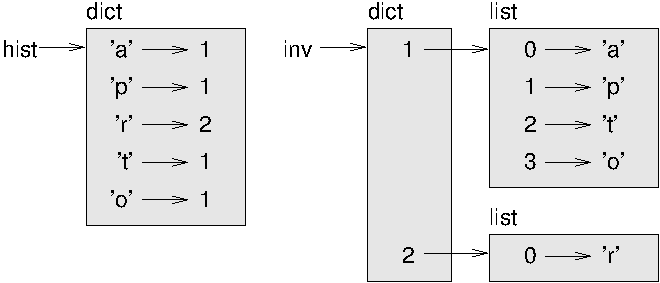
\includegraphics[scale=0.8]{../source/figs/dict1.pdf}}
\caption{State diagram.}
\label{fig.dict1}
\end{figure}

Figure~\ref{fig.dict1} is a state diagram showing {\tt hist} and {\tt inverse}.
A dictionary is represented as a box with the type {\tt dict} above it
and the key-value pairs inside.  If the values are integers, floats or
strings, I draw them inside the box, but I usually draw lists
outside the box, just to keep the diagram simple.
\index{state diagram}
\index{diagram!state}

Lists can be values in a dictionary, as this example shows, but they
cannot be keys.  Here's what happens if you try:
\index{TypeError}
\index{exception!TypeError}


\begin{verbatim}
>>> t = [1, 2, 3]
>>> d = dict()
>>> d[t] = 'oops'
Traceback (most recent call last):
  File "<stdin>", line 1, in ?
TypeError: list objects are unhashable
\end{verbatim}
%
I mentioned earlier that a dictionary is implemented using
a hashtable and that means that the keys have to be {\bf hashable}.
\index{hash function}
\index{hashable}

A {\bf hash} is a function that takes a value (of any kind)
and returns an integer.  Dictionaries use these integers,
called hash values, to store and look up key-value pairs.
\index{immutability}

This system works fine if the keys are immutable.  But if the
keys are mutable, like lists, bad things happen.  For example,
when you create a key-value pair, Python hashes the key and
stores it in the corresponding location.  If you modify the
key and then hash it again, it would go to a different location.
In that case you might have two entries for the same key,
or you might not be able to find a key.  Either way, the
dictionary wouldn't work correctly.

That's why keys have to be hashable, and why mutable types like
lists aren't.  The simplest way to get around this limitation is to
use tuples, which we will see in the next chapter.

Since dictionaries are mutable, they can't be used as keys,
but they {\em can} be used as values.


\section{Memos}
\label{memoize}

If you played with the {\tt fibonacci} function from
Section~\ref{one.more.example}, you might have noticed that the bigger
the argument you provide, the longer the function takes to run.
Furthermore, the run time increases quickly.
\index{fibonacci function}
\index{function!fibonacci}

To understand why, consider Figure~\ref{fig.fibonacci}, which shows
the {\bf call graph} for {\tt fibonacci} with {\tt n=4}:

\begin{figure}
\centerline
{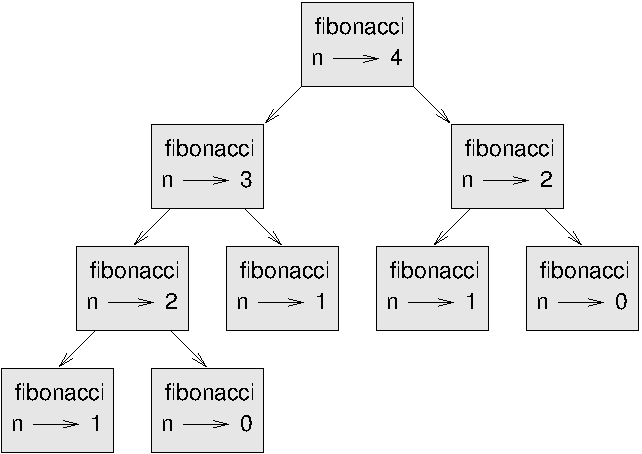
\includegraphics[scale=0.7]{../source/figs/fibonacci.pdf}}
\caption{Call graph.}
\label{fig.fibonacci}
\end{figure}

A call graph shows a set of function frames, with lines connecting each
frame to the frames of the functions it calls.  At the top of the
graph, {\tt fibonacci} with {\tt n=4} calls {\tt fibonacci} with {\tt
n=3} and {\tt n=2}.  In turn, {\tt fibonacci} with {\tt n=3} calls
{\tt fibonacci} with {\tt n=2} and {\tt n=1}.  And so on.
\index{function frame}
\index{frame}
\index{call graph}

Count how many times {\tt fibonacci(0)} and {\tt fibonacci(1)} are
called.  This is an inefficient solution to the problem, and it gets
worse as the argument gets bigger.
\index{memo}

One solution is to keep track of values that have already been
computed by storing them in a dictionary.  A previously computed value
that is stored for later use is called a {\bf memo}.  Here is a
``memoized'' version of {\tt fibonacci}:

\begin{verbatim}
known = {0:0, 1:1}

def fibonacci(n):
    if n in known:
        return known[n]

    res = fibonacci(n-1) + fibonacci(n-2)
    known[n] = res
    return res
\end{verbatim}
%
{\tt known} is a dictionary that keeps track of the Fibonacci
numbers we already know.  It starts with
two items: 0 maps to 0 and 1 maps to 1.

Whenever {\tt fibonacci} is called, it checks {\tt known}.
If the result is already there, it can return
immediately.  Otherwise it has to
compute the new value, add it to the dictionary, and return it.

If you run this version of {\tt fibonacci} and compare it with
the original, you will find that it is much faster.



\section{Global variables}
\index{global variable}
\index{variable!global}

In the previous example, {\tt known} is created outside the function,
so it belongs to the special frame called \verb"__main__".
Variables in \verb"__main__" are sometimes called {\bf global}
because they can be accessed from any function.  Unlike local
variables, which disappear when their function ends, global variables
persist from one function call to the next.
\index{flag}

It is common to use global variables for {\bf flags}; that is,
boolean variables that indicate (``flag'') whether a condition
is true.  For example, some programs use
a flag named {\tt verbose} to control the level of detail in the
output:

\begin{verbatim}
verbose = True

def example1():
    if verbose:
        print('Running example1')
\end{verbatim}
%
If you try to reassign a global variable, you might be surprised.
The following example is supposed to keep track of whether the
function has been called:
\index{reassignment}

\begin{verbatim}
been_called = False

def example2():
    been_called = True         # WRONG
\end{verbatim}
%
But if you run it you will see that the value of \verb"been_called"
doesn't change.  The problem is that {\tt example2} creates a new local
variable named \verb"been_called".  The local variable goes away when
the function ends, and has no effect on the global variable.
\index{global statement}
\index{statement!global}
\index{declaration}

To reassign a global variable inside a function you have to
{\bf declare} the global variable before you use it:

\begin{verbatim}
been_called = False

def example2():
    global been_called
    been_called = True
\end{verbatim}
%
The {\bf global statement} tells the interpreter
something like, ``In this function, when I say \verb"been_called", I
mean the global variable; don't create a local one.''
\index{update!global variable}
\index{global variable!update}

Here's an example that tries to update a global variable:

\begin{verbatim}
count = 0

def example3():
    count = count + 1          # WRONG
\end{verbatim}
%
If you run it you get:
\index{UnboundLocalError}
\index{exception!UnboundLocalError}

\begin{verbatim}
UnboundLocalError: local variable 'count' referenced before assignment
\end{verbatim}
%
Python assumes that {\tt count} is local, and under that assumption
you are reading it before writing it.  The solution, again,
is to declare {\tt count} global.
\index{counter}

\begin{verbatim}
def example3():
    global count
    count += 1
\end{verbatim}
%
If a global variable refers to a mutable value, you can modify
the value without declaring the variable:
\index{mutability}

\begin{verbatim}
known = {0:0, 1:1}

def example4():
    known[2] = 1
\end{verbatim}
%
So you can add, remove and replace elements of a global list or
dictionary, but if you want to reassign the variable, you
have to declare it:

\begin{verbatim}
def example5():
    global known
    known = dict()
\end{verbatim}
%
Global variables can be useful, but if you have a lot of them,
and you modify them frequently, they can make programs
hard to debug.


\section{Debugging}
\index{debugging}

As you work with bigger datasets it can become unwieldy to
debug by printing and checking the output by hand.  Here are some
suggestions for debugging large datasets:

\begin{description}

\item[Scale down the input:] If possible, reduce the size of the
dataset.  For example if the program reads a text file, start with
just the first 10 lines, or with the smallest example you can find.
You can either edit the files themselves, or (better) modify the
program so it reads only the first {\tt n} lines.

If there is an error, you can reduce {\tt n} to the smallest
value that manifests the error, and then increase it gradually
as you find and correct errors.

\item[Check summaries and types:] Instead of printing and checking the
entire dataset, consider printing summaries of the data: for example,
the number of items in a dictionary or the total of a list of numbers.

A common cause of runtime errors is a value that is not the right
type.  For debugging this kind of error, it is often enough to print
the type of a value.

\item[Write self-checks:]  Sometimes you can write code to check
for errors automatically.  For example, if you are computing the
average of a list of numbers, you could check that the result is
not greater than the largest element in the list or less than
the smallest.  This is called a ``sanity check'' because it detects
results that are ``insane''.
\index{sanity check}
\index{consistency check}

Another kind of check compares the results of two different
computations to see if they are consistent.  This is called a
``consistency check''.

\item[Format the output:] Formatting debugging output
can make it easier to spot an error.  We saw an example in
Section~\ref{factdebug}.  The {\tt pprint} module provides
a {\tt pprint} function that displays built-in types in
a more human-readable format ({\tt pprint} stands for
``pretty print'').
\index{pretty print}
\index{pprint module}
\index{module!pprint}

\end{description}

Again, time you spend building scaffolding can reduce
the time you spend debugging.
\index{scaffolding}


\section{Glossary}

\begin{description}

\item[mapping:] A relationship in which each element of one set
corresponds to an element of another set.
\index{mapping}

\item[dictionary:] A mapping from keys to their
corresponding values.
\index{dictionary}

\item[key-value pair:] The representation of the mapping from
a key to a value.
\index{key-value pair}

\item[item:] In a dictionary, another name for a key-value
  pair.
\index{item!dictionary}

\item[key:] An object that appears in a dictionary as the
first part of a key-value pair.
\index{key}

\item[value:] An object that appears in a dictionary as the
second part of a key-value pair.  This is more specific than
our previous use of the word ``value''.
\index{value}

\item[implementation:] A way of performing a computation.
\index{implementation}

\item[hashtable:] The algorithm used to implement Python
dictionaries.
\index{hashtable}

\item[hash function:] A function used by a hashtable to compute the
location for a key.
\index{hash function}

\item[hashable:] A type that has a hash function.  Immutable
types like integers,
floats and strings are hashable; mutable types like lists and
dictionaries are not.
\index{hashable}

\item[lookup:] A dictionary operation that takes a key and finds
the corresponding value.
\index{lookup}

\item[reverse lookup:] A dictionary operation that takes a value and finds
one or more keys that map to it.
\index{reverse lookup}

\item[raise statement:]  A statement that (deliberately) raises an exception.
\index{raise statement}
\index{statement!raise}

\item[singleton:] A list (or other sequence) with a single element.
\index{singleton}

\item[call graph:] A diagram that shows every frame created during
the execution of a program, with an arrow from each caller to
each callee.
\index{call graph}
\index{diagram!call graph}

\item[memo:] A computed value stored to avoid unnecessary future
computation.
\index{memo}

\item[global variable:]  A variable defined outside a function.  Global
variables can be accessed from any function.
\index{global variable}

\item[global statement:]  A statement that declares a variable name
global.
\index{global statement}
\index{statement!global}

\item[flag:] A boolean variable used to indicate whether a condition
is true.
\index{flag}

\item[declaration:] A statement like {\tt global} that tells the
interpreter something about a variable.
\index{declaration}

\end{description}


\section{Exercises}

\begin{exercise}
\label{wordlist2}
\index{set membership}
\index{membership!set}

Write a function that reads the words in {\tt words.txt} and
stores them as keys in a dictionary.  It doesn't matter what the
values are.  Then you can use the {\tt in} operator
as a fast way to check whether a string is in
the dictionary.

If you did Exercise~\ref{wordlist1}, you can compare the speed
of this implementation with the list {\tt in} operator and the
bisection search.

\end{exercise}


\begin{exercise}
\label{setdefault}

Read the documentation of the dictionary method {\tt setdefault}
and use it to write a more concise version of \verb"invert_dict".
Solution: \url{http://thinkpython2.com/code/invert_dict.py}.
\index{setdefault method}
\index{method!setdefault}

\end{exercise}


\begin{exercise}
Memoize the Ackermann function from Exercise~\ref{ackermann} and see if
memoization makes it possible to evaluate the function with bigger
arguments.  Hint: no.
Solution: \url{http://thinkpython2.com/code/ackermann_memo.py}.
\index{Ackermann function}
\index{function!ack}

\end{exercise}



\begin{exercise}
\index{duplicate}

If you did Exercise~\ref{duplicate}, you already have
a function named \verb"has_duplicates" that takes a list
as a parameter and returns {\tt True} if there is any object
that appears more than once in the list.

Use a dictionary to write a faster, simpler version of
\verb"has_duplicates".
Solution: \url{http://thinkpython2.com/code/has_duplicates.py}.

\end{exercise}


\begin{exercise}
\label{exrotatepairs}
\index{letter rotation}
\index{rotation!letters}

Two words are ``rotate pairs'' if you can rotate one of them
and get the other (see \verb"rotate_word" in Exercise~\ref{exrotate}).

Write a program that reads a wordlist and finds all the rotate
pairs.  Solution: \url{http://thinkpython2.com/code/rotate_pairs.py}.

\end{exercise}


\begin{exercise}
\index{Car Talk}
\index{Puzzler}

Here's another Puzzler from {\em Car Talk}
(\url{http://www.cartalk.com/content/puzzlers}):

\begin{quote}
This was sent in by a fellow named Dan O'Leary. He came upon a common
one-syllable, five-letter word recently that has the following unique
property. When you remove the first letter, the remaining letters form
a homophone of the original word, that is a word that sounds exactly
the same. Replace the first letter, that is, put it back and remove
the second letter and the result is yet another homophone of the
original word. And the question is, what's the word?

Now I'm going to give you an example that doesn't work. Let's look at
the five-letter word, `wrack.' W-R-A-C-K, you know like to `wrack with
pain.' If I remove the first letter, I am left with a four-letter
word, 'R-A-C-K.' As in, `Holy cow, did you see the rack on that buck!
It must have been a nine-pointer!' It's a perfect homophone. If you
put the `w' back, and remove the `r,' instead, you're left with the
word, `wack,' which is a real word, it's just not a homophone of the
other two words.

But there is, however, at least one word that Dan and we know of,
which will yield two homophones if you remove either of the first two
letters to make two, new four-letter words. The question is, what's
the word?
\end{quote}
\index{homophone}
\index{reducible word}
\index{word, reducible}

You can use the dictionary from Exercise~\ref{wordlist2} to check
whether a string is in the word list.

To check whether two words are homophones, you can use the CMU
Pronouncing Dictionary.  You can download it from
\url{http://www.speech.cs.cmu.edu/cgi-bin/cmudict} or from
\url{http://thinkpython2.com/code/c06d} and you can also download
\url{http://thinkpython2.com/code/pronounce.py}, which provides a function
named \verb"read_dictionary" that reads the pronouncing dictionary and
returns a Python dictionary that maps from each word to a string that
describes its primary pronunciation.

Write a program that lists all the words that solve the Puzzler.
Solution: \url{http://thinkpython2.com/code/homophone.py}.

\end{exercise}




%🍁% \chapter{Tuples | 元组}
\chapter{元组}
\label{tuplechap}

%🍁% This chapter presents one more built-in type, the tuple, and then
%🍁% shows how lists, dictionaries, and tuples work together.
%🍁% I also present a useful feature for variable-length argument lists,
%🍁% the gather and scatter operators.
%🍁%
%🍁% One note: there is no consensus on how to pronounce ``tuple''.
%🍁% Some people say ``tuh-ple'', which rhymes with ``supple''.  But
%🍁% in the context of programming, most people say ``too-ple'', which
%🍁% rhymes with ``quadruple''.

本章介绍另一个内建的类型 --- 元组\footnote{值得注意的是, ``tuple''并没有统一的发音, 有些人读``tuh-ple'', 音律类似于``supple'';而有人读``too-ple''音律类似于``quadruple''。  }, 同时说明如何结合使用列表、字典和元组。
后面的章节会介绍关于 可变长度参数列表 的有用功能, 以及\emph{汇集} 和 \emph{分散}操作。

%🍁% \section{Tuples are immutable | 元组是不可变的}
\section{元组是不可变的}
\index{tuple}  \index{type!tuple}  \index{sequence}

%🍁% A tuple is a sequence of values.  The values can be any type, and
%🍁% they are indexed by integers, so in that respect tuples are a lot
%🍁% like lists.  The important difference is that tuples are immutable.
\index{mutability}  \index{immutability}

元组是一组\emph{值}的序列。
其中的值可以是任意类型, 使用整数索引其位置, 因此元组与列表非常相似。
而重要的不同之处在于元组的不可变性。

%🍁% Syntactically, a tuple is a comma-separated list of values:

语法上,元组是用逗号隔开一系列值的列表:

\begin{lstlisting}
>>> t = 'a', 'b', 'c', 'd', 'e'
\end{lstlisting}
%
%🍁% Although it is not necessary, it is common to enclose tuples in
%🍁% parentheses:

虽然并非必须, 元组通常用括号括起来:

\index{parentheses!tuples in}

\begin{lstlisting}
>>> t = ('a', 'b', 'c', 'd', 'e')
\end{lstlisting}
%
%🍁% To create a tuple with a single element, you have to include a final
%🍁% comma:

使用单一元素建立元组时, 需要在结尾使用一个逗号:

\index{singleton}
\index{tuple!singleton}

\begin{lstlisting}
>>> t1 = 'a',
>>> type(t1)
<class 'tuple'>
\end{lstlisting}
%
%🍁% A value in parentheses is not a tuple:

将值放置在括号中并不会创建元组:

\begin{lstlisting}
>>> t2 = ('a')
>>> type(t2)
<class 'str'>
\end{lstlisting}
%
%🍁% Another way to create a tuple is the built-in function {\tt tuple}.
%🍁% With no argument, it creates an empty tuple:
\index{tuple function}
\index{function!tuple}

另一个建立元组的方法是使用内建函数 \li{tuple}。
在没有参数传递时它会产生一个空元组。

\begin{lstlisting}
>>> t = tuple()
>>> t
()
\end{lstlisting}

%
%🍁% If the argument is a sequence (string, list or tuple), the result
%🍁% is a tuple with the elements of the sequence:

如果实参是一个序列(字符串、列表或者元组), 结果将是包含序列内元素的一个元组。

\begin{lstlisting}
>>> t = tuple('lupins')
>>> t
('l', 'u', 'p', 'i', 'n', 's')
\end{lstlisting}
%
%🍁% Because {\tt tuple} is the name of a built-in function, you should
%🍁% avoid using it as a variable name.

因为 \li{tuple} 是内建函数名, 所以应该避免将它用于变量名。


%🍁% Most list operators also work on tuples.  The bracket operator
%🍁% indexes an element:

列表的大多数操作同样也适用于元组。  方括号运算符将索引一个元素:

\index{bracket operator}
\index{operator!bracket}

\begin{lstlisting}
>>> t = ('a', 'b', 'c', 'd', 'e')
>>> t[0]
'a'
\end{lstlisting}
%
%🍁% And the slice operator selects a range of elements.

切片操作可以选取一个范围内的元素:
\index{slice operator}  \index{operator!slice}
\index{tuple!slice}  \index{slice!tuple}
\index{切片操作符}  \index{操作符!切片}
\index{元组!切片}  \index{切片!元组}

\begin{lstlisting}
>>> t[1:3]
('b', 'c')
\end{lstlisting}
%
%🍁% But if you try to modify one of the elements of the tuple, you get
%🍁% an error:

但是, 如果你试更改图元组中的一个元素, 会得到错误信息:

\index{exception!TypeError}  \index{TypeError}
\index{item assignment}  \index{assignment!item}

\begin{lstlisting}
>>> t[0] = 'A'
TypeError: object doesn't support item assignment
\end{lstlisting}

%
%🍁% Because tuples are immutable, you can't modify the elements.  But you
%🍁% can replace one tuple with another:

因为元组是不可变的, 您无法改变其中的元素。
但是可以使用其他元组替换现有元组:

\begin{lstlisting}
>>> t = ('A',) + t[1:]
>>> t
('A', 'b', 'c', 'd', 'e')
\end{lstlisting}
%
%🍁% This statement makes a new tuple and then makes {\tt t} refer to it.

这个语句创建了一个新元组, 然后让 \li{t} 引用该元组。

%🍁% The relational operators work with tuples and other sequences;
%🍁% Python starts by comparing the first element from each
%🍁% sequence.  If they are equal, it goes on to the next elements,
%🍁% and so on, until it finds elements that differ.  Subsequent
%🍁% elements are not considered (even if they are really big).

关系型操作也适用于元组和其他序列;
Python 会首先比较序列中的第一个元素, 如果它们相等, 就继续比较下一组元素,
以此类推, 直至比值不同。
其后的元素(即便是差异很大)也不会再参与比较。

\index{comparison!tuple}
\index{tuple!comparison}

\begin{lstlisting}
>>> (0, 1, 2) < (0, 3, 4)
True
>>> (0, 1, 2000000) < (0, 3, 4)
True
\end{lstlisting}


%🍁% \section{Tuple assignment | 元组赋值}
\section{元组赋值}
\label{tuple.assignment} \index{tuple!assignment} \index{assignment!tuple}
\index{swap pattern} \index{pattern!swap}

%🍁% It is often useful to swap the values of two variables.
%🍁% With conventional assignments, you have to use a temporary
%🍁% variable.  For example, to swap {\tt a} and {\tt b}:

两个变量互换值的操作通常很有用。
按照传统的赋值方法, 你需要使用一个临时变量。
例如为了交换 \li{a}和 \li{b} 的值:

\begin{lstlisting}
>>> temp = a
>>> a = b
>>> b = temp
\end{lstlisting}
%
%🍁% This solution is cumbersome; {\bf tuple assignment} is more elegant:

这个方法很繁琐;通过{\bf 元组赋值}来实现更为优雅:

\begin{lstlisting}
>>> a, b = b, a
\end{lstlisting}
%
%🍁% The left side is a tuple of variables; the right side is a tuple of
%🍁% expressions.  Each value is assigned to its respective variable.
%🍁% All the expressions on the right side are evaluated before any
%🍁% of the assignments.

等号左侧是变量组成的元组;右侧是表达式组成的元组。
每个值都被赋给了对应的变量。
变量被重新赋值前, 将先对右侧的表达式进行求值。

%🍁% The number of variables on the left and the number of
%🍁% values on the right have to be the same:

使用元组赋值, 左右两侧变量数必须相同:

\index{exception!ValueError}  \index{ValueError}

\begin{lstlisting}
>>> a, b = 1, 2, 3
ValueError: too many values to unpack
\end{lstlisting}
%
%🍁% More generally, the right side can be any kind of sequence
%🍁% (string, list or tuple).  For example, to split an email address
%🍁% into a user name and a domain, you could write:

一般说来, 元组赋值时右侧表达式可以是任意类型(字符串、列表或者元组)的序列。  例如, 将一个电子邮箱地址分成用户名和域名, 你可以:

\index{split method}  \index{method!split}
\index{email address}

\begin{lstlisting}
>>> addr = 'monty@python.org'
>>> uname, domain = addr.split('@')
\end{lstlisting}

%
%🍁% The return value from {\tt split} is a list with two elements;
%🍁% the first element is assigned to {\tt uname}, the second to
%🍁% {\tt domain}.

 \li{split}函数返回的对象是一个包含两个元素的列表;第一个元素被赋给了 \li{uname}的变量, 第二个被赋给了 \li{domain}。

\begin{lstlisting}
>>> uname
'monty'
>>> domain
'python.org'
\end{lstlisting}
%

%🍁% \section{Tuples as return values | 元组作为返回值}
\section{元组作为返回值}
\index{tuple} \index{value!tuple} \index{return value!tuple}
\index{function, tuple as return value}

%🍁% Strictly speaking, a function can only return one value, but
%🍁% if the value is a tuple, the effect is the same as returning
%🍁% multiple values.  For example, if you want to divide two integers
%🍁% and compute the quotient and remainder, it is inefficient to
%🍁% compute {\tt x/y} and then {\tt x\%y}.  It is better to compute
%🍁% them both at the same time.

严格地说, 一个函数只能返回一个值, 但是如果这个返回值是元组, 其效果等同于返回多个值。  例如, 你想对两个整数做除法, 计算出商和余数, 依次计算出 \li{x/y}和 \li{x%y}是很低效的。
同时计算出这两个值更好。
\index{divmod}

%🍁% The built-in function {\tt divmod} takes two arguments and
%🍁% returns a tuple of two values, the quotient and remainder.
%🍁% You can store the result as a tuple:

内建函数\href{https://docs.python.org/3/library/functions.html#divmod}{ \li{divmod}}接受两个参数, 返回包含两个值的元组 --- 商和余数。
可以使用元组来存储返回值:

\begin{lstlisting}
>>> t = divmod(7, 3)
>>> t
(2, 1)
\end{lstlisting}

%
%🍁% Or use tuple assignment to store the elements separately:

或者使用元组赋值分别存储它们:

\index{tuple assignment}  \index{assignment!tuple}

\begin{lstlisting}
>>> quot, rem = divmod(7, 3)
>>> quot
2
>>> rem
1
\end{lstlisting}

%
%🍁% Here is an example of a function that returns a tuple:

下面是另一个返回元组作为结果的函数例子:

\begin{lstlisting}
def min_max(t):
    return min(t), max(t)
\end{lstlisting}

%
%🍁% {\tt max} and {\tt min} are built-in functions that find
%🍁% the largest and smallest elements of a sequence.  \verb"min_max"
%🍁% computes both and returns a tuple of two values.

 \li{max} 和  \li{min} 是用于找出一组元素序列中最大值和最小值的内建函数, \li{min_max}函数同时计算出这两个值, 并返回二者组成的元组。
\index{max function} \index{function!max}
\index{min function} \index{function!min}


%🍁% \section{Variable-length argument tuples | 可变长度参数元组}
\section{可变长度参数元组}
\label{gather}
\index{variable-length argument tuple} \index{argument!variable-length tuple}
\index{gather} \index{parameter!gather} \index{argument!gather}

%🍁% Functions can take a variable number of arguments.  A parameter
%🍁% name that begins with {\tt *} {\bf gathers} arguments into
%🍁% a tuple.  For example, {\tt printall}
%🍁% takes any number of arguments and prints them:

函数可以接受可变数量的参数。  以 {\bf *} 开头的形参将输入的参数 \emph{汇集} 到一个元组中。
例如, \li{printall} 可以接受任意数量的参数, 并将它们打印出来:

\begin{lstlisting}
def printall(*args):
    print(args)
\end{lstlisting}

%
%🍁% The gather parameter can have any name you like, but {\tt args} is
%🍁% conventional.  Here's how the function works:

汇集的形参可以使用任意名字, 但是习惯使用 \li{args}。
以下是这个函数的调用效果:

\begin{lstlisting}
>>> printall(1, 2.0, '3')
(1, 2.0, '3')
\end{lstlisting}

%
%🍁% The complement of gather is {\bf scatter}.  If you have a
%🍁% sequence of values and you want to pass it to a function
%🍁% as multiple arguments, you can use the {\tt *} operator.
%🍁% For example, {\tt divmod} takes exactly two arguments; it
%🍁% doesn't work with a tuple:

与汇集相对的是\emph{分散}{\bf scatter}。
如果你有一个值的序列, 并且希望将其作为多个参数传递给一个函数,
你可以使用运算符 \li{*}。
例如, \li{divmod} 需要接受两个实参;一个元组则无法作为参数传递进去:

\index{scatter} \index{argument scatter} \index{TypeError}
\index{exception!TypeError}

\begin{lstlisting}
>>> t = (7, 3)
>>> divmod(t)
TypeError: divmod expected 2 arguments, got 1
\end{lstlisting}

%
%🍁% But if you scatter the tuple, it works:

但是如果将这个元组分散, 它就可以被传递进函数:

\begin{lstlisting}
>>> divmod(*t)
(2, 1)
\end{lstlisting}

%
%🍁% Many of the built-in functions use
%🍁% variable-length argument tuples.  For example, {\tt max}
%🍁% and {\tt min} can take any number of arguments:

多数内建函数使用可变长度参数元组。
例如, \li{max} 和  \li{min} 可以接受任意数量的实参。

\index{max function} \index{function!max}
\index{min function} \index{function!min}

\begin{lstlisting}
>>> max(1, 2, 3)
3
\end{lstlisting}

%
%🍁% But {\tt sum} does not.

但是求和操作 \li{sum} 不行:
\index{sum function} \index{function!sum}

\begin{lstlisting}
>>> sum(1, 2, 3)
TypeError: sum expected at most 2 arguments, got 3
\end{lstlisting}

%
%🍁% As an exercise, write a function called {\tt sumall} that takes any number
%🍁% of arguments and returns their sum.

我们尝试编写一个叫做  \li{sumall}的函数作为练习,
使它能够接受任何数量的传参并返回它们的和。


%🍁% \section{Lists and tuples | 列表和元组}
\section{列表和元组}
\index{zip function} \index{function!zip}

%🍁% {\tt zip} is a built-in function that takes two or more sequences and
%🍁% returns a list of tuples where each tuple contains one
%🍁% element from each sequence.  The name of the function refers to
%🍁% a zipper, which joins and interleaves two rows of teeth.

 \li{zip} 是一个内建函数, 可以接受将两个或多个序列组, 并返回一个元组列表,
其中每个元组包含了各个序列中相对位置的一个元素。
这个函数的名称来自名词拉链 (zipper), 后者将两片链齿连接拼合在一起。


%🍁% This example zips a string and a list:

下面的示例对一个字符串和列表使用 \li{zip} 函数:

\begin{lstlisting}
>>> s = 'abc'
>>> t = [0, 1, 2]
>>> zip(s, t)
<zip object at 0x7f7d0a9e7c48>
\end{lstlisting}

%
%🍁% The result is a {\bf zip object} that knows how to iterate through
%🍁% the pairs.  The most common use of {\tt zip} is in a {\tt for} loop:

输出的结果是一个 {\em \li{zip} 对象}, 包含了如何对其中元素进行迭代的信息。
\li{zip} 函数最常用于 \li{for} 循环:

\begin{lstlisting}
>>> for pair in zip(s, t):
...     print(pair)
...
('a', 0)
('b', 1)
('c', 2)
\end{lstlisting}

%
%🍁% A zip object is a kind of {\bf iterator}, which is any object
%🍁% that iterates through a sequence.  Iterators are similar to lists in some
%🍁% ways, but unlike lists, you can't use an index to select an element from
%🍁% an iterator.

\href{https://docs.python.org/3/library/functions.html#zip}{\li{zip}}对象是一个友善的 {\bf 迭代器}, 是指任何一种能够按照某个序列迭代的对象。  迭代器在某些方面与列表非常相似, 不同之处在于, 你无法通过索引来选择迭代器中的某个元素。
\index{iterator} \index{迭代器}

%🍁% If you want to use list operators and methods, you can
%🍁% use a zip object to make a list:

如果你想使用列表操作符和方法, 你可以通过 \li {zip}对象创造一个列表:

\begin{lstlisting}
>>> list(zip(s, t))
[('a', 0), ('b', 1), ('c', 2)]
\end{lstlisting}

%
%🍁% The result is a list of tuples; in this example, each tuple contains
%🍁% a character from the string and the corresponding element from
%🍁% the list.

结果就是一个包含若干元组的列表;在这个例子中, 每个元组又包含了字符串中的一个字符和列表 \li {t} 中对应的一个元素。
\index{list!of tuples}

%🍁% If the sequences are not the same length, the result has the
%🍁% length of the shorter one.

如果用于创建的序列长度不一, 返回的对象的长度以最短序列的长度为准。

\begin{lstlisting}
>>> list(zip('Anne', 'Elk'))
[('A', 'E'), ('n', 'l'), ('n', 'k')]
\end{lstlisting}

%
%🍁% You can use tuple assignment in a {\tt for} loop to traverse a list of
%🍁% tuples:

你可以在 \li{for} 循环中使用元组赋值, 遍历包含元组的列表:

\index{traversal} \index{tuple assignment} \index{assignment!tuple}

\begin{lstlisting}
t = [('a', 0), ('b', 1), ('c', 2)]
for letter, number in t:
    print(number, letter)
\end{lstlisting}

%
%🍁% Each time through the loop, Python selects the next tuple in
%🍁% the list and assigns the elements to {\tt letter} and
%🍁% {\tt number}.  The output of this loop is:

循环中的每次执行, Python 会选择列表中的下一个元组,
并将其内容赋给  \li{letter} 和  \li{number}。
因此循环打印的输出会是这样:
\index{loop}

\begin{lstlisting}
0 a
1 b
2 c
\end{lstlisting}

%
%🍁% If you combine {\tt zip}, {\tt for} and tuple assignment, you get a
%🍁% useful idiom for traversing two (or more) sequences at the same
%🍁% time.  For example, \verb"has_match" takes two sequences, {\tt t1} and
%🍁% {\tt t2}, and returns {\tt True} if there is an index {\tt i}
%🍁% such that {\tt t1[i] == t2[i]}:

如果将 \li{zip}、 \li{for}循环和元组赋值结合起来使用,
你会得到一个可以同时遍历两个(甚至多个)序列的惯用法。
例如, \li{has_match} 接受两个序列, \li{t1} 和 \li{t2},
如果存在索引满足 \li{t1[i] == t2[i]} \li {i}, 则返回 \li{True}:
\index{for loop}

\begin{lstlisting}
def has_match(t1, t2):
    for x, y in zip(t1, t2):
        if x == y:
            return True
    return False
\end{lstlisting}

%
%🍁% If you need to traverse the elements of a sequence and their
%🍁% indices, you can use the built-in function {\tt enumerate}:

如果需要遍历一个序列的元素以及它们的索引号, 你可以使用内建函数 \li{enumerate}:
\index{traversal} \index{enumerate function} \index{function!enumerate}

\begin{lstlisting}
for index, element in enumerate('abc'):
    print(index, element)
\end{lstlisting}

%
%🍁% The result from {\tt enumerate} is an enumerate object, which
%🍁% iterates a sequence of pairs; each pair contains an index (starting
%🍁% from 0) and an element from the given sequence.
%🍁% In this example, the output is

\li{enumerate} 的返回结果是一个 枚举对象(enumerate object),
它可基于一个包含若干个 \emph{对} 的序列进行迭代,
每个对包含了(从0开始计数)的索引号和给定序列中对应的元素。
在刚才的例子中, 对应的输出结果会和前例一样:

\begin{lstlisting}
0 a
1 b
2 c
\end{lstlisting}

%
%🍁% Again.
\index{iterator}    \index{object!enumerate}    \index{enumerate object}


%🍁% \section{Dictionaries and tuples | 字典和元组}
\section{字典和元组}
\label{dictuple}
\index{dictionary} \index{items method}
\index{method!items} \index{key-value pair}

%🍁% Dictionaries have a method called {\tt items} that returns a sequence of
%🍁% tuples, where each tuple is a key-value pair.

字典对象有一个内建方法叫做 \href{https://docs.python.org/3/library/stdtypes.html?highlight=items#dict.items}{ \li{itmes} }, 它返回由多个元组组成的序列, 其中每个元组是一个键值对。

\begin{lstlisting}
>>> d = {'a':0, 'b':1, 'c':2}
>>> t = d.items()
>>> t
dict_items([('c', 2), ('a', 0), ('b', 1)])
\end{lstlisting}

%
%🍁% The result is a \verb"dict_items" object, which is an iterator that
%🍁% iterates the key-value pairs.  You can use it in a {\tt for} loop
%🍁% like this:

其结果是一个 \li{dict_itmes} 对象, 这是一个对键值对进行迭代的迭代器。
你可以在 \li{for} 循环中像这样使用它:
\index{iterator}

\begin{lstlisting}
>>> for key, value in d.items():
...     print(key, value)
...
c 2
a 0
b 1
\end{lstlisting}

%
%🍁% As you should expect from a dictionary, the items are in no
%🍁% particular order.

由于是字典生成的对象, 你应该猜到了这些项是无序的。

%🍁% Going in the other direction, you can use a list of tuples to
%🍁% initialize a new dictionary:

另一方面, 你可以使用元组的列表初始化一个新的字典:
\index{dictionary!initialize}

\begin{lstlisting}
>>> t = [('a', 0), ('c', 2), ('b', 1)]
>>> d = dict(t)
>>> d
{'a': 0, 'c': 2, 'b': 1}
\end{lstlisting}

%🍁% Combining {\tt dict} with {\tt zip} yields a concise way
%🍁% to create a dictionary:

将 \li{dict} 和 \li{zip}结合使用, 可以很简洁地创建一个字典:
\index{zip function!use with dict}

\begin{lstlisting}
>>> d = dict(zip('abc', range(3)))
>>> d
{'a': 0, 'c': 2, 'b': 1}
\end{lstlisting}

%
%🍁% The dictionary method {\tt update} also takes a list of tuples
%🍁% and adds them, as key-value pairs, to an existing dictionary.


字典的 \li{update} 方法也接受元组的列表, 并作为键-值对把它们添加到已有的字典中。

\index{update method}  \index{method!update}
\index{traverse!dictionary}  \index{dictionary!traversal}

%🍁% It is common to use tuples as keys in dictionaries (primarily because
%🍁% you can't use lists).  For example, a telephone directory might map
%🍁% from last-name, first-name pairs to telephone numbers.  Assuming
%🍁% that we have defined {\tt last}, {\tt first} and {\tt number}, we
%🍁% could write:

在字典中使用元组作为键(主要因为无法使用列表)的做法很常见。
例如, 一个电话簿可能会基于用户的姓-名对, 来映射至号码。
假设我们已经定义了 \li{last} 、 \li{first} 和 \li{number} 三个变量,
我们可以这样实现映射:

\index{tuple!as key in dictionary}
\index{hashable}

\begin{lstlisting}
directory[last, first] = number
\end{lstlisting}

%
%🍁% The expression in brackets is a tuple.  We could use tuple
%🍁% assignment to traverse this dictionary.

方括号中的表达式是一个元组。
我们可以通过元组赋值来遍历这个字典:
\index{tuple!in brackets}

\begin{lstlisting}
for last, first in directory:
    print(first, last, directory[last,first])
\end{lstlisting}

%
%🍁% This loop traverses the keys in {\tt directory}, which are tuples.  It
%🍁% assigns the elements of each tuple to {\tt last} and {\tt first}, then
%🍁% prints the name and corresponding telephone number.

该循环遍历 电话簿 \li{directory}中的键, 它们其实是元组。
循环将元组的元素赋给 \li{last} 和 \li{first} , 然后打印出姓名和对应的电话号码。

%🍁% There are two ways to represent tuples in a state diagram.  The more
%🍁% detailed version shows the indices and elements just as they appear in
%🍁% a list.  For example, the tuple \verb"('Cleese', 'John')" would appear
%🍁% as in Figure~\ref{fig.tuple1}.

在状态图中有两种表示元组的方法。
更详细的版本是, 索引号和对应元素就像列表一样存放在元组中。
例如, 元组 \li{('Cleese', 'John')}可像图~\ref{fig.tuple1}中那样存放。
\index{state diagram} \index{diagram!state}

\begin{figure}
\centerline
{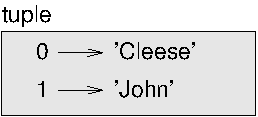
\includegraphics[scale=0.8]{../source/figs/tuple1.pdf}}
\caption{State diagram.}
\label{fig.tuple1}
\end{figure}

%🍁% But in a larger diagram you might want to leave out the
%🍁% details.  For example, a diagram of the telephone directory might
%🍁% appear as in Figure~\ref{fig.dict2}.

在更大的图中, 我们忽略这些细节。
该电话簿的状态图可能如图~\ref{fig.dict2}所示。

\begin{figure}
\centerline
{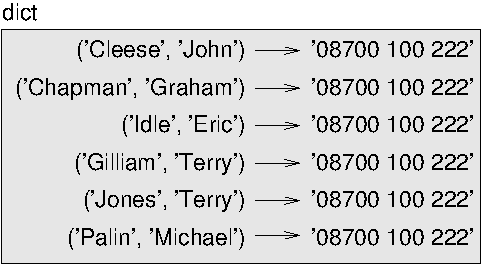
\includegraphics[scale=0.8]{../source/figs/dict2.pdf}}
\caption{State diagram.}
\label{fig.dict2}
\end{figure}

%🍁% Here the tuples are shown using Python syntax as a graphical
%🍁% shorthand.  The telephone number in the diagram is the complaints line
%🍁% for the BBC, so please don't call it.

因此, Python风格的元组用法可用这两幅图来描述。
此图中的电话号码是 BBC 的投诉热线, 请不要拨打它。


%🍁% \section{Sequences of sequences | 序列嵌套}
\section{序列嵌套}
\index{sequence}

%🍁% I have focused on lists of tuples, but almost all of the examples in
%🍁% this chapter also work with lists of lists, tuples of tuples, and
%🍁% tuples of lists.  To avoid enumerating the possible combinations, it
%🍁% is sometimes easier to talk about sequences of sequences.

我已经介绍了包含元组的列表, 事实上, 本章大多数例子也适用于列表嵌套列表、 元组嵌套元组, 以及元组嵌套列表。
为了避免 --- 穷举这类可能的嵌套组合, 我们简称为序列嵌套。

%🍁% In many contexts, the different kinds of sequences (strings, lists and
%🍁% tuples) can be used interchangeably.  So how should you choose one
%🍁% over the others?

在很多情况下, 不同类型的序列(字符串、列表、元组)可以互换使用。  因此, 我们如何选用合适的嵌套对象呢?
\index{string} \index{list} \index{tuple} \index{mutability}
\index{immutability}

%🍁% To start with the obvious, strings are more limited than other
%🍁% sequences because the elements have to be characters.  They are
%🍁% also immutable.  If you need the ability to change the characters
%🍁% in a string (as opposed to creating a new string), you might
%🍁% want to use a list of characters instead.

首先, 显而易见的是, 字符串比其他序列的限制更多, 因为它的所有元素都是字符, 且字符串不可变。
如果你希望能够改变字符在字符串中的位置, 使用列表嵌套字符比较合适。

%🍁% Lists are more common than tuples, mostly because they are mutable.
%🍁% But there are a few cases where you might prefer tuples:

列表比元组更常见, 这源于它们可变性的易用。
但是有些情况下, 你会更倾向于使用元组:

%🍁% \begin{enumerate}
%🍁%
%🍁% \item In some contexts, like a {\tt return} statement, it is
%🍁% syntactically simpler to create a tuple than a list.
%🍁%
%🍁% \item If you want to use a sequence as a dictionary key, you
%🍁% have to use an immutable type like a tuple or string.
%🍁%
%🍁% \item If you are passing a sequence as an argument to a function,
%🍁% using tuples reduces the potential for unexpected behavior
%🍁% due to aliasing.
%🍁%
%🍁% \end{enumerate}

\begin{enumerate}

\item 在一些情况下(例如 \li{return}语句), 从句式上生成一个元组比列表要简单。

\item 如果你想使用一个序列作为字典的键, 那么你必须使用元组或字符串这样的不可变类型。

\item 如果你向函数传入一个序列作为参数, 那么使用元组以降低由于别名而产生的意外行为的可能性。

\end{enumerate}

%🍁% Because tuples are immutable, they don't provide methods like {\tt
%🍁%   sort} and {\tt reverse}, which modify existing lists.  But Python
%🍁% provides the built-in function {\tt sorted}, which takes any sequence
%🍁% and returns a new list with the same elements in sorted order, and
%🍁% {\tt reversed}, which takes a sequence and returns an iterator that
%🍁% traverses the list in reverse order.

正由于元组的不可变性, 它们没有类似 \li{sort} 和 \li{reverser} 这样修改现有列表的方法。
然而 Python 提供了内建函数  \li{sorted}, 用于对任意序列排序并输出相同元素的列表, 以及  \li {reversed}, 用于对序列逆向排序并生成一个可以遍历的迭代器。

\index{sorted function} \index{function!sorted} \index{reversed function}
\index{function!reversed} \index{iterator}


%🍁% \section{Debugging  |  调试}
\section{调试}
\index{debugging} \index{data structure}
\index{shape error} \index{error!shape}

%🍁% Lists, dictionaries and tuples are examples of {\bf data
%🍁%   structures}; in this chapter we are starting to see compound data
%🍁% structures, like lists of tuples, or dictionaries that contain tuples
%🍁% as keys and lists as values.  Compound data structures are useful, but
%🍁% they are prone to what I call {\bf shape errors}; that is, errors
%🍁% caused when a data structure has the wrong type, size, or structure.
%🍁% For example, if you are expecting a list with one integer and I
%🍁% give you a plain old integer (not in a list), it won't work.

列表、  字典 和 元组 都是 {\em 数据结构} ({\bf data structures});
本章中, 我们开始接触到 复合数据结构 ({\bf compound data structures}),
如: 列表嵌套元组, 又如使用元组作为键而列表作为值的字典。
复合数据结构非常实用, 然而使用时容易出现所谓的 {\em 形状错误} ({\bf shape errors}), 也就是说由于数据结构的类型、大小或结构问题而引发的错误。
例如, 当你希望使用封装整数的列表时却用成了没被列表包含的一串整数。
\index{structshape module} \index{module!structshape}

%🍁% To help debug these kinds of errors, I have written a module
%🍁% called {\tt structshape} that provides a function, also called
%🍁% {\tt structshape}, that takes any kind of data structure as
%🍁% an argument and returns a string that summarizes its shape.
%🍁% You can download it from \url{http://thinkpython2.com/code/structshape.py}

为了方面调试这类错误, 我编写了一个叫做  \li{structshape} 的模块,
它提供了一个名为 \li{structshape} 的函数, 可以接受任意类型的数据结构作为实参, 然后返回一个描述它形状的字符串。
你可以在\href{http://thinkpython2.com/code/structshape.py}{这里}下载到它(\url{http://thinkpython2.com/code/structshape.py})。

%🍁% Here's the result for a simple list:

下面是用该模块调试一个简单列表的示例:

\begin{lstlisting}
>>> from structshape import structshape
>>> t = [1, 2, 3]
>>> structshape(t)
'list of 3 int'
\end{lstlisting}

%
%🍁% A fancier program might write ``list of 3 int{\em s}'', but it
%🍁% was easier not to deal with plurals.  Here's a list of lists:

更完美的程序应该显示 ``list of 3 int{\em s}'', 但是忽略英文复数使程序简单的多。
我们再看一个列表嵌套的例子:

\begin{lstlisting}
>>> t2 = [[1,2], [3,4], [5,6]]
>>> structshape(t2)
'list of 3 list of 2 int'
\end{lstlisting}

%
%🍁% If the elements of the list are not the same type,
%🍁% {\tt structshape} groups them, in order, by type:

如果列表内的元素不是相同类型, \li{structshape} 会按照类型的顺序进行分组:

\begin{lstlisting}
>>> t3 = [1, 2, 3, 4.0, '5', '6', [7], [8], 9]
>>> structshape(t3)
'list of (3 int, float, 2 str, 2 list of int, int)'
\end{lstlisting}

%
%🍁% Here's a list of tuples:

下面是一个元组列表的例子:

\begin{lstlisting}
>>> s = 'abc'
>>> lt = list(zip(t, s))
>>> structshape(lt)
'list of 3 tuple of (int, str)'
\end{lstlisting}

%
%🍁% And here's a dictionary with 3 items that map integers to strings.

下面是一个字典的例子, 其中包含三个将整数映射至字符串的项:

\begin{lstlisting}
>>> d = dict(lt)
>>> structshape(d)
'dict of 3 int->str'
\end{lstlisting}

%
%🍁% If you are having trouble keeping track of your data structures,
%🍁% {\tt structshape} can help.

如果你在追踪数据结构的类型上遇到了困难, 可以使用 \li{structshape} 来帮助分析。

%🍁% \section{Glossary  |  术语表}
\section{术语表}

\begin{description}

%🍁% \item[tuple:] An immutable sequence of elements.

\item[元组 (tuple):] 一组不可变的元素的序列。
\index{tuple}

%🍁% \item[tuple assignment:] An assignment with a sequence on the
%🍁% right side and a tuple of variables on the left.  The right
%🍁% side is evaluated and then its elements are assigned to the
%🍁% variables on the left.

\item[元组赋值 (tuple assignment):] 一种赋值方式, 通过等号右侧的序列向等号左侧的一组变量的元组进行赋值。
右侧的表达式先求值, 然后其元素被赋值给左侧元组中对应的变量。
\index{tuple assignment} \index{assignment!tuple}

%🍁% \item[gather:] The operation of assembling a variable-length
%🍁% argument tuple.
\index{gather}

\item[汇集 (gather):] 组装可变长度变量元组的一种操作。

%🍁% \item[scatter:] The operation of treating a sequence as a list of
%🍁% arguments.
\index{scatter}

\item[分散 (scatter):] 将一个序列变换成一个参数列表的操作。


%🍁% \item[zip object:] The result of calling a built-in function {\tt zip};
%🍁% an object that iterates through a sequence of tuples.

\item[zip 对象:] 使用内建函数 \li{zip} 所返回的结果; 它是一个可通过元组序列逐个迭代的对象。
\index{zip object} \index{object!zip}

%🍁% \item[iterator:] An object that can iterate through a sequence, but
%🍁% which does not provide list operators and methods.

\item[迭代器 (iterator):]: 一个可以对序列进行迭代的对象, 但是并不提供列表操作符和方法。
\index{iterator}

%🍁% \item[data structure:] A collection of related values, often
%🍁% organized in lists, dictionaries, tuples, etc.

\item[数据结构 (data structure):] 一个由关联值组成的数据集合, 通常组织成列表、 字典、 元组等。
\index{data structure}

%🍁% \item[shape error:] An error caused because a value has the
%🍁% wrong shape; that is, the wrong type or size.

\item[形状错误:] 由于某个值的形状出错, 而导致的错误; 即拥有错误的类型或大小。
\index{shape}

\end{description}


%🍁% \section{Exercises  |  练习}

\section{练习}

\begin{exercise}
%🍁% Write a function called \verb"most_frequent" that takes a string and
%🍁% prints the letters in decreasing order of frequency.  Find text
%🍁% samples from several different languages and see how letter frequency
%🍁% varies between languages.  Compare your results with the tables at
%🍁% \url{http://en.wikipedia.org/wiki/Letter_frequencies}.  Solution:
%🍁% \url{http://thinkpython2.com/code/most_frequent.py}.

编写一个名为 {\em  \li{most_frequent}} 的函数,
接受一个字符串, 并按字符出现的频率 降序打印字母。
找一些不同语言的文本样本, 来试试看不同语言之间字母频率的区别。
将你的结果和维基百科的
\href{http://en.wikipedia.org/wiki/Letter_frequencies}{字母频率} 进行比较。

\href{http://thinkpython2.com/code/most_frequent.py}{参考答案}

\index{letter frequency} \index{frequency!letter}
\index{字母频度} \index{频度!字母}

\index{维基百科}


\end{exercise}


\begin{exercise}
\label{anagrams}
\index{anagram set}  \index{set!anagram}

%🍁% More anagrams!
易位构词游戏 {\em (\href{https://zh.wikipedia.org/wiki/%E6%98%93%E4%BD%8D%E6%9E%84%E8%AF%8D%E6%B8%B8%E6%88%8F}{anagrams})}!

\begin{enumerate}

%🍁% \item Write a program
%🍁% that reads a word list from a file (see Section~\ref{wordlist}) and
%🍁% prints all the sets of words that are anagrams.
%🍁%
%🍁% Here is an example of what the output might look like:
%🍁%
%🍁% \begin{lstlisting}
%🍁% ['deltas', 'desalt', 'lasted', 'salted', 'slated', 'staled']
%🍁% ['retainers', 'ternaries']
%🍁% ['generating', 'greatening']
%🍁% ['resmelts', 'smelters', 'termless']
%🍁% \end{lstlisting}
%🍁%
%🍁% %
%🍁% Hint: you might want to build a dictionary that maps from a
%🍁% collection of letters to a list of words that can be spelled with those
%🍁% letters.  The question is, how can you represent the collection of
%🍁% letters in a way that can be used as a key?
%🍁%
%🍁% \item Modify the previous program so that it prints the longest list
%🍁% of anagrams first, followed by the second longest, and so on.
%🍁% \index{Scrabble}
%🍁% \index{bingo}
%🍁%
%🍁% \item In Scrabble a ``bingo'' is when you play all seven tiles in
%🍁% your rack, along with a letter on the board, to form an eight-letter
%🍁% word.  What collection of 8 letters forms the most possible bingos?
%🍁% Hint: there are seven.
%🍁%
%🍁% % (7, ['angriest', 'astringe', 'ganister', 'gantries', 'granites',
%🍁% % 'ingrates', 'rangiest'])
%🍁%
%🍁% Solution: \url{http://thinkpython2.com/code/anagram_sets.py}.



\item 编写一个程序, 使之能从文件中读取单词的列表 (参考章节~{\em \ref{wordlist}}) 并且打印出所有符合异位构词的组合。

下面是一个输出异位构词的样例:

{\em
\begin{lstlisting}
['deltas', 'desalt', 'lasted', 'salted', 'slated', 'staled']
['retainers', 'ternaries']
['generating', 'greatening']
['resmelts', 'smelters', 'termless']
\end{lstlisting}
}

提示:也许你可以建立一个字典, 用于映射一个字符集合到一个该集合可异位构词的词汇集合。

\item 改写前面的程序, 使之首先打印包含异位构词数量最多的词汇列表, 第二多次之, 依次按异位构词数量排列。

\item \href{https://en.wikipedia.org/wiki/Scrabble}{{\em Scrabble}} \href{https://zh.wikipedia.org/wiki/Scrabble}{拼字游戏} 中, 游戏胜利{\em (``bingo'')}指的是你利用手里的全部七个字母, 与图版上的那个字母一起构成一个 {\em 8} 个字母的单词。  哪八个字母能够达成最多的 {\em ``bingo''?} 提示:最多有7种胜利方式。

\href{http://thinkpython2.com/code/anagram_sets.py}{参考答案}

\end{enumerate}

\end{exercise}

\begin{exercise}
\index{metathesis}

%🍁% Two words form a ``metathesis pair'' if you can transform one into the
%🍁% other by swapping two letters; for example, ``converse'' and
%🍁% ``conserve''.  Write a program that finds all of the metathesis pairs
%🍁% in the dictionary.  Hint: don't test all pairs of words, and don't
%🍁% test all possible swaps.  Solution:
%🍁% \url{http://thinkpython2.com/code/metathesis.py}.  Credit: This
%🍁% exercise is inspired by an example at \url{http://puzzlers.org}.

如果两个单词中的某一单词可以通过调换两个字母变为另一个, 这两个单词就构成了
``换位对 {\em (metatheisi pair)}''; 比如 {\em ``converse''} 和 {\em ``conserve''}。
编写一个程序, 找出给定字典里所有的 ``换位对''。\footnote{提示: 不用测试所有的单词组合, 也不用测试所有的字母调换组合。  }

\href{http://thinkpython2.com/code/metathesis.py}{参考答案}

\footnote{这个练习受\href{http://puzzlers.org}{http://puzzlers.org}的案例启发而成。  }

\end{exercise}


\begin{exercise}
\index{Car Talk}
\index{Puzzler}

%🍁% Here's another Car Talk Puzzler
%🍁% (\url{http://www.cartalk.com/content/puzzlers}):
%🍁%
%🍁% \begin{quote}
%🍁% What is the longest English word, that remains a valid English word,
%🍁% as you remove its letters one at a time?
%🍁%
%🍁% Now, letters can be removed from either end, or the middle, but you
%🍁% can't rearrange any of the letters. Every time you drop a letter, you
%🍁% wind up with another English word. If you do that, you're eventually
%🍁% going to wind up with one letter and that too is going to be an
%🍁% English word---one that's found in the dictionary. I want to know
%🍁% what's the longest word and how many letters does it
%🍁% have?
%🍁%
%🍁% I'm going to give you a little modest example: Sprite. Ok? You start
%🍁% off with sprite, you take a letter off, one from the interior of the
%🍁% word, take the r away, and we're left with the word spite, then we
%🍁% take the e off the end, we're left with spit, we take the s off, we're
%🍁% left with pit, it, and I.
%🍁% \end{quote}

另一个来自 {\em Car Talk} 的字谜题 \href{http://www.cartalk.com/content/puzzlers}{{\em car talk puzzler}} :

\begin{quote}

如果你每一次从单词中删掉一个字母以后, 剩下的字符仍然能构成一个单词, 请问世界上符合条件的最长单词是什么?

注意, 被删掉的字母可以位于首尾或是中间, 但不允许重新去排列剩下的字母。
每次移除一个字母后 , 你会得到一个新单词。
这样一直下去, 最终你只剩一个字母, 并且它也是一个单词——可以在字典中查到。  我想知道, 符合条件的最长单词是什么?它由多少个字母构成?

我先给出一个短小的例子: {\em ``Sprite''}, 一开始是 {\em sprite} , 我们可以拿掉中间的 {\em `r'} 从而获得单词 {\em spite}, 拿去字母 {\em `e'} 得到 {\em spit}, 再去掉 {\em `s'} 剩下 {\em pit}, {\em it}, 最后 {\em I}。
\end{quote}

\index{reducible word} \index{word, reducible}

%🍁% Write a program to find all words that can be reduced in this way,
%🍁% and then find the longest one.
%🍁%
%🍁% This exercise is a little more challenging than most, so here are
%🍁% some suggestions:

%🍁% \begin{enumerate}
%🍁%
%🍁% \item You might want to write a function that takes a word and
%🍁%   computes a list of all the words that can be formed by removing one
%🍁%   letter.  These are the ``children'' of the word.
%🍁% \index{recursive definition}
%🍁% \index{definition!recursive}
%🍁%
%🍁% \item Recursively, a word is reducible if any of its children
%🍁% are reducible.  As a base case, you can consider the empty
%🍁% string reducible.
%🍁%
%🍁% \item The wordlist I provided, {\tt words.txt}, doesn't
%🍁% contain single letter words.  So you might want to add
%🍁% ``I'', ``a'', and the empty string.
%🍁%
%🍁% \item To improve the performance of your program, you might want
%🍁% to memoize the words that are known to be reducible.
%🍁%
%🍁% \end{enumerate}
%🍁%
%🍁% Solution: \url{http://thinkpython2.com/code/reducible.py}.

编写一个程序, 按照这种规则找到所有可以缩减的单词, 然后看看其中哪个词最长。

这道题比大部分的习题都要难, 所以我给出一些建议:

\begin{enumerate}
\item 可能你需要写一个函数将输入单词的所有``子词''(即拿掉一个字母后所有可能的新词)以列表形式输出。
\index{recursive definition} \index{definition!recursive}

\item 递归地看, 如果单词的子词之一也可缩减, 那么这个单词也可被缩减。
我们可以将空字符串视作也可以缩减, 视其为基础情形。

\item 我们提供的词汇表 {\em (\li{words.txt})} 并未包含诸如 {\em `I'}、 {\em `a'} 这样的单个字母词汇, 因此你可能需要加上它们。

\item 为了提高你程序的性能, 你可能需要暂存 {\em (memorize)} 好已被发现的可被缩词的词汇。

\end{enumerate}

\href{http://thinkpython2.com/code/reducible.py}{参考答案}

\end{exercise}




%\begin{exercise}
%\url{http://en.wikipedia.org/wiki/Word_Ladder}
%\end{exercise}







\chapter{Case study: data structure selection}

At this point you have learned about Python's core data structures,
and you have seen some of the algorithms that use them.
If you would like to know more about algorithms, this might be a good
time to read Chapter~\ref{algorithms}.
But you don't have to read it before you go on; you can read
it whenever you are interested.

This chapter presents a case study with exercises that let
you think about choosing data structures and practice using them.


\section{Word frequency analysis}
\label{analysis}

As usual, you should at least attempt the exercises
before you read my solutions.

\begin{exercise}

Write a program that reads a file, breaks each line into
words, strips whitespace and punctuation from the words, and
converts them to lowercase.
\index{string module}
\index{module!string}

Hint: The {\tt string} module provides a string named {\tt whitespace},
which contains space, tab, newline, etc., and {\tt
  punctuation} which contains the punctuation characters.  Let's see
if we can make Python swear:

\begin{verbatim}
>>> import string
>>> string.punctuation
'!"#$%&'()*+,-./:;<=>?@[\]^_`{|}~'
\end{verbatim}
%
Also, you might consider using the string methods {\tt strip},
{\tt replace} and {\tt translate}.
\index{strip method}
\index{method!strip}
\index{replace method}
\index{method!replace}
\index{translate method}
\index{method!translate}

\end{exercise}


\begin{exercise}
\index{Project Gutenberg}

Go to Project Gutenberg (\url{http://gutenberg.org}) and download
your favorite out-of-copyright book in plain text format.
\index{plain text}
\index{text!plain}

Modify your program from the previous exercise to read the book
you downloaded, skip over the header information at the beginning
of the file, and process the rest of the words as before.

Then modify the program to count the total number of words in
the book, and the number of times each word is used.
\index{word frequency}
\index{frequency!word}

Print the number of different words used in the book.  Compare
different books by different authors, written in different eras.
Which author uses the most extensive vocabulary?
\end{exercise}


\begin{exercise}

Modify the program from the previous exercise to print the
20 most frequently used words in the book.

\end{exercise}


\begin{exercise}

Modify the previous program to read a word list (see
Section~\ref{wordlist}) and then print all the words in the book that
are not in the word list.  How many of them are typos?  How many of
them are common words that {\em should} be in the word list, and how
many of them are really obscure?

\end{exercise}


\section{Random numbers}
\index{random number}
\index{number, random}
\index{deterministic}
\index{pseudorandom}

Given the same inputs, most computer programs generate the same
outputs every time, so they are said to be {\bf deterministic}.
Determinism is usually a good thing, since we expect the same
calculation to yield the same result.  For some applications, though,
we want the computer to be unpredictable.  Games are an obvious
example, but there are more.

Making a program truly nondeterministic turns out to be difficult,
but there are ways to make it at least seem nondeterministic.  One of
them is to use algorithms that generate {\bf pseudorandom} numbers.
Pseudorandom numbers are not truly random because they are generated
by a deterministic computation, but just by looking at the numbers it
is all but impossible to distinguish them from random.
\index{random module}
\index{module!random}

The {\tt random} module provides functions that generate
pseudorandom numbers (which I will simply call ``random'' from
here on).
\index{random function}
\index{function!random}

The function {\tt random} returns a random float
between 0.0 and 1.0 (including 0.0 but not 1.0).  Each time you
call {\tt random}, you get the next number in a long series.  To see a
sample, run this loop:

\begin{verbatim}
import random

for i in range(10):
    x = random.random()
    print(x)
\end{verbatim}
%
The function {\tt randint} takes parameters {\tt low} and
{\tt high} and returns an integer between {\tt low} and
{\tt high} (including both).
\index{randint function}
\index{function!randint}

\begin{verbatim}
>>> random.randint(5, 10)
5
>>> random.randint(5, 10)
9
\end{verbatim}
%
To choose an element from a sequence at random, you can use
{\tt choice}:
\index{choice function}
\index{function!choice}

\begin{verbatim}
>>> t = [1, 2, 3]
>>> random.choice(t)
2
>>> random.choice(t)
3
\end{verbatim}
%
The {\tt random} module also provides functions to generate
random values from continuous distributions including
Gaussian, exponential, gamma, and a few more.

\begin{exercise}
\index{histogram!random choice}

Write a function named \verb"choose_from_hist" that takes
a histogram as defined in Section~\ref{histogram} and returns a
random value from the histogram, chosen with probability
in proportion to frequency.  For example, for this histogram:

\begin{verbatim}
>>> t = ['a', 'a', 'b']
>>> hist = histogram(t)
>>> hist
{'a': 2, 'b': 1}
\end{verbatim}
%
your function should return \verb"'a'" with probability $2/3$ and \verb"'b'"
with probability $1/3$.
\end{exercise}


\section{Word histogram}

You should attempt the previous exercises before you go on.
You can download my solution from
 \url{http://thinkpython2.com/code/analyze_book1.py}.  You will
also need \url{http://thinkpython2.com/code/emma.txt}.

Here is a program that reads a file and builds a histogram of the
words in the file:
\index{histogram!word frequencies}

\begin{verbatim}
import string

def process_file(filename):
    hist = dict()
    fp = open(filename)
    for line in fp:
        process_line(line, hist)
    return hist

def process_line(line, hist):
    line = line.replace('-', ' ')

    for word in line.split():
        word = word.strip(string.punctuation + string.whitespace)
        word = word.lower()
        hist[word] = hist.get(word, 0) + 1

hist = process_file('emma.txt')
\end{verbatim}
%
This program reads {\tt emma.txt}, which contains the text of {\em
  Emma} by Jane Austen.
\index{Austin, Jane}

\verb"process_file" loops through the lines of the file,
passing them one at a time to \verb"process_line".  The histogram
{\tt hist} is being used as an accumulator.
\index{accumulator!histogram}
\index{traversal}

\verb"process_line" uses the string method {\tt replace} to replace
hyphens with spaces before using {\tt split} to break the line into a
list of strings.  It traverses the list of words and uses {\tt strip}
and {\tt lower} to remove punctuation and convert to lower case.  (It
is a shorthand to say that strings are ``converted''; remember that
strings are immutable, so methods like {\tt strip} and {\tt lower}
return new strings.)

Finally, \verb"process_line" updates the histogram by creating a new
item or incrementing an existing one.
\index{update!histogram}

To count the total number of words in the file, we can add up
the frequencies in the histogram:

\begin{verbatim}
def total_words(hist):
    return sum(hist.values())
\end{verbatim}
%
The number of different words is just the number of items in
the dictionary:

\begin{verbatim}
def different_words(hist):
    return len(hist)
\end{verbatim}
%
Here is some code to print the results:

\begin{verbatim}
print('Total number of words:', total_words(hist))
print('Number of different words:', different_words(hist))
\end{verbatim}
%
And the results:

\begin{verbatim}
Total number of words: 161080
Number of different words: 7214
\end{verbatim}
%

\section{Most common words}

To find the most common words, we can make a list of tuples,
where each tuple contains a word and its frequency,
and sort it.

The following function takes a histogram and returns a list of
word-frequency tuples:

\begin{verbatim}
def most_common(hist):
    t = []
    for key, value in hist.items():
        t.append((value, key))

    t.sort(reverse=True)
    return t
\end{verbatim}

In each tuple, the frequency appears first, so the resulting list is
sorted by frequency.  Here is a loop that prints the ten most common
words:

\begin{verbatim}
t = most_common(hist)
print('The most common words are:')
for freq, word in t[:10]:
    print(word, freq, sep='\t')
\end{verbatim}
%
I use the keyword argument {\tt sep} to tell {\tt print} to use a tab
character as a ``separator'', rather than a space, so the second
column is lined up.  Here are the results from {\em Emma}:

\begin{verbatim}
The most common words are:
to      5242
the     5205
and     4897
of      4295
i       3191
a       3130
it      2529
her     2483
was     2400
she     2364
\end{verbatim}
%
This code can be simplified using the {\tt key} parameter of
the {\tt sort} function.  If you are curious, you can read about it
at \url{https://wiki.python.org/moin/HowTo/Sorting}.


\section{Optional parameters}
\index{optional parameter}
\index{parameter!optional}

We have seen built-in functions and methods that take optional
arguments.  It is possible to write programmer-defined functions
with optional arguments, too.  For example, here is a function that
prints the most common words in a histogram
\index{programmer-defined function}
\index{function!programmer defined}

\begin{verbatim}
def print_most_common(hist, num=10):
    t = most_common(hist)
    print('The most common words are:')
    for freq, word in t[:num]:
        print(word, freq, sep='\t')
\end{verbatim}

The first parameter is required; the second is optional.
The {\bf default value} of {\tt num} is 10.
\index{default value}
\index{value!default}

If you only provide one argument:

\begin{verbatim}
print_most_common(hist)
\end{verbatim}

{\tt num} gets the default value.  If you provide two arguments:

\begin{verbatim}
print_most_common(hist, 20)
\end{verbatim}

{\tt num} gets the value of the argument instead.  In other
words, the optional argument {\bf overrides} the default value.
\index{override}

If a function has both required and optional parameters, all
the required parameters have to come first, followed by the
optional ones.


\section{Dictionary subtraction}
\label{dictsub}
\index{dictionary!subtraction}
\index{subtraction!dictionary}

Finding the words from the book that are not in the word list
from {\tt words.txt} is a problem you might recognize as set
subtraction; that is, we want to find all the words from one
set (the words in the book) that are not in the other (the
words in the list).

{\tt subtract} takes dictionaries {\tt d1} and {\tt d2} and returns a
new dictionary that contains all the keys from {\tt d1} that are not
in {\tt d2}.  Since we don't really care about the values, we
set them all to None.

\begin{verbatim}
def subtract(d1, d2):
    res = dict()
    for key in d1:
        if key not in d2:
            res[key] = None
    return res
\end{verbatim}
%
To find the words in the book that are not in {\tt words.txt},
we can use \verb"process_file" to build a histogram for
{\tt words.txt}, and then subtract:

\begin{verbatim}
words = process_file('words.txt')
diff = subtract(hist, words)

print("Words in the book that aren't in the word list:")
for word in diff.keys():
    print(word, end=' ')
\end{verbatim}
%
Here are some of the results from {\em Emma}:

\begin{verbatim}
Words in the book that aren't in the word list:
rencontre jane's blanche woodhouses disingenuousness
friend's venice apartment ...
\end{verbatim}
%
Some of these words are names and possessives.  Others, like
``rencontre'', are no longer in common use.  But a few are common
words that should really be in the list!

\begin{exercise}
\index{set}
\index{type!set}

Python provides a data structure called {\tt set} that provides many
common set operations.  You can read about them in Section~\ref{sets},
or read the documentation at
\url{http://docs.python.org/3/library/stdtypes.html#types-set}.

Write a program that uses set subtraction to find words in the book
that are not in the word list.  Solution:
\url{http://thinkpython2.com/code/analyze_book2.py}.

\end{exercise}


\section{Random words}
\label{randomwords}
\index{histogram!random choice}

To choose a random word from the histogram, the simplest algorithm
is to build a list with multiple copies of each word, according
to the observed frequency, and then choose from the list:

\begin{verbatim}
def random_word(h):
    t = []
    for word, freq in h.items():
        t.extend([word] * freq)

    return random.choice(t)
\end{verbatim}
%
The expression {\tt [word] * freq} creates a list with {\tt freq}
copies of the string {\tt word}.  The {\tt extend}
method is similar to {\tt append} except that the argument is
a sequence.

This algorithm works, but it is not very efficient; each time you
choose a random word, it rebuilds the list, which is as big as
the original book.  An obvious improvement is to build the list
once and then make multiple selections, but the list is still big.

An alternative is:

\begin{enumerate}

\item Use {\tt keys} to get a list of the words in the book.

\item Build a list that contains the cumulative sum of the word
  frequencies (see Exercise~\ref{cumulative}).  The last item
  in this list is the total number of words in the book, $n$.

\item Choose a random number from 1 to $n$.  Use a bisection search
  (See Exercise~\ref{bisection}) to find the index where the random
  number would be inserted in the cumulative sum.

\item Use the index to find the corresponding word in the word list.

\end{enumerate}

\begin{exercise}
\label{randhist}
\index{algorithm}

Write a program that uses this algorithm to choose a random word from
the book.  Solution:
\url{http://thinkpython2.com/code/analyze_book3.py}.

\end{exercise}



\section{Markov analysis}
\label{markov}
\index{Markov analysis}

If you choose words from the book at random, you can get a
sense of the vocabulary, but you probably won't get a sentence:

\begin{verbatim}
this the small regard harriet which knightley's it most things
\end{verbatim}
%
A series of random words seldom makes sense because there
is no relationship between successive words.  For example, in
a real sentence you would expect an article like ``the'' to
be followed by an adjective or a noun, and probably not a verb
or adverb.

One way to measure these kinds of relationships is Markov
analysis, which
characterizes, for a given sequence of words, the probability of the
words that might come next.  For example, the song {\em Eric, the Half a
  Bee} begins:

\begin{quote}
Half a bee, philosophically, \\
Must, ipso facto, half not be. \\
But half the bee has got to be \\
Vis a vis, its entity. D'you see? \\
\\
But can a bee be said to be \\
Or not to be an entire bee \\
When half the bee is not a bee \\
Due to some ancient injury? \\
\end{quote}
%
In this text,
the phrase ``half the'' is always followed by the word ``bee'',
but the phrase ``the bee'' might be followed by either
``has'' or ``is''.
\index{prefix}
\index{suffix}
\index{mapping}

The result of Markov analysis is a mapping from each prefix
(like ``half the'' and ``the bee'') to all possible suffixes
(like ``has'' and ``is'').
\index{random text}
\index{text!random}

Given this mapping, you can generate a random text by
starting with any prefix and choosing at random from the
possible suffixes.  Next, you can combine the end of the
prefix and the new suffix to form the next prefix, and repeat.

For example, if you start with the prefix ``Half a'', then the
next word has to be ``bee'', because the prefix only appears
once in the text.  The next prefix is ``a bee'', so the
next suffix might be ``philosophically'', ``be'' or ``due''.

In this example the length of the prefix is always two, but
you can do Markov analysis with any prefix length.

\begin{exercise}

Markov analysis:

\begin{enumerate}

\item Write a program to read a text from a file and perform Markov
analysis.  The result should be a dictionary that maps from
prefixes to a collection of possible suffixes.  The collection
might be a list, tuple, or dictionary; it is up to you to make
an appropriate choice.  You can test your program with prefix
length two, but you should write the program in a way that makes
it easy to try other lengths.

\item Add a function to the previous program to generate random text
based on the Markov analysis.  Here is an example from {\em Emma}
with prefix length 2:

\begin{quote}
He was very clever, be it sweetness or be angry, ashamed or only
amused, at such a stroke. She had never thought of Hannah till you
were never meant for me?" "I cannot make speeches, Emma:" he soon cut
it all himself.
\end{quote}

For this example, I left the punctuation attached to the words.
The result is almost syntactically correct, but not quite.
Semantically, it almost makes sense, but not quite.

What happens if you increase the prefix length?  Does the random
text make more sense?

\item Once your program is working, you might want to try a mash-up:
if you combine text from two or more books, the random
text you generate will blend the vocabulary and phrases from
the sources in interesting ways.
\index{mash-up}

\end{enumerate}

Credit: This case study is based on an example from Kernighan and
Pike, {\em The Practice of Programming}, Addison-Wesley, 1999.

\end{exercise}

You should attempt this exercise before you go on; then you can can
download my solution from \url{http://thinkpython2.com/code/markov.py}.
You will also need \url{http://thinkpython2.com/code/emma.txt}.


\section{Data structures}
\index{data structure}

Using Markov analysis to generate random text is fun, but there is
also a point to this exercise: data structure selection.  In your
solution to the previous exercises, you had to choose:

\begin{itemize}

\item How to represent the prefixes.

\item How to represent the collection of possible suffixes.

\item How to represent the mapping from each prefix to
the collection of possible suffixes.

\end{itemize}

The last one is easy: a dictionary is the obvious choice
for a mapping from keys to corresponding values.

For the prefixes, the most obvious options are string,
list of strings, or tuple of strings.

For the suffixes,
one option is a list; another is a histogram (dictionary).
\index{implementation}

How should you choose?  The first step is to think about
the operations you will need to implement for each data structure.
For the prefixes, we need to be able to remove words from
the beginning and add to the end.  For example, if the current
prefix is ``Half a'', and the next word is ``bee'', you need
to be able to form the next prefix, ``a bee''.
\index{tuple!as key in dictionary}

Your first choice might be a list, since it is easy to add
and remove elements, but we also need to be able to use the
prefixes as keys in a dictionary, so that rules out lists.
With tuples, you can't append or remove, but you can use
the addition operator to form a new tuple:

\begin{verbatim}
def shift(prefix, word):
    return prefix[1:] + (word,)
\end{verbatim}
%
{\tt shift} takes a tuple of words, {\tt prefix}, and a string,
{\tt word}, and forms a new tuple that has all the words
in {\tt prefix} except the first, and {\tt word} added to
the end.

For the collection of suffixes, the operations we need to
perform include adding a new suffix (or increasing the frequency
of an existing one), and choosing a random suffix.

Adding a new suffix is equally easy for the list implementation
or the histogram.  Choosing a random element from a list
is easy; choosing from a histogram is harder to do
efficiently (see Exercise~\ref{randhist}).

So far we have been talking mostly about ease of implementation,
but there are other factors to consider in choosing data structures.
One is run time.  Sometimes there is a theoretical reason to expect
one data structure to be faster than other; for example, I mentioned
that the {\tt in} operator is faster for dictionaries than for lists,
at least when the number of elements is large.

But often you don't know ahead of time which implementation will
be faster.  One option is to implement both of them and see which
is better.  This approach is called {\bf benchmarking}.  A practical
alternative is to choose the data structure that is
easiest to implement, and then see if it is fast enough for the
intended application.  If so, there is no need to go on.  If not,
there are tools, like the {\tt profile} module, that can identify
the places in a program that take the most time.
\index{benchmarking}
\index{profile module}
\index{module!profile}

The other factor to consider is storage space.  For example, using a
histogram for the collection of suffixes might take less space because
you only have to store each word once, no matter how many times it
appears in the text.  In some cases, saving space can also make your
program run faster, and in the extreme, your program might not run at
all if you run out of memory.  But for many applications, space is a
secondary consideration after run time.

One final thought: in this discussion, I have implied that
we should use one data structure for both analysis and generation.  But
since these are separate phases, it would also be possible to use one
structure for analysis and then convert to another structure for
generation.  This would be a net win if the time saved during
generation exceeded the time spent in conversion.


\section{Debugging}
\index{debugging}

When you are debugging a program, and especially if you are
working on a hard bug, there are five things to try:

\begin{description}

\item[Reading:] Examine your code, read it back to yourself, and
check that it says what you meant to say.

\item[Running:] Experiment by making changes and running different
versions.  Often if you display the right thing at the right place
in the program, the problem becomes obvious, but sometimes you have to
build scaffolding.

\item[Ruminating:] Take some time to think!  What kind of error
is it: syntax, runtime, or semantic?  What information can you get from
the error messages, or from the output of the program?  What kind of
error could cause the problem you're seeing?  What did you change
last, before the problem appeared?

\item[Rubberducking:] If you explain the problem to someone else, you
  sometimes find the answer before you finish asking the question.
  Often you don't need the other person; you could just talk to a rubber
  duck.  And that's the origin of the well-known strategy called {\bf
    rubber duck debugging}.  I am not making this up; see
  \url{https://en.wikipedia.org/wiki/Rubber_duck_debugging}.

\item[Retreating:] At some point, the best thing to do is back
off, undoing recent changes, until you get back to a program that
works and that you understand.  Then you can start rebuilding.

\end{description}

Beginning programmers sometimes get stuck on one of these activities
and forget the others.  Each activity comes with its own failure
mode.
\index{typographical error}

For example, reading your code might help if the problem is a
typographical error, but not if the problem is a conceptual
misunderstanding.  If you don't understand what your program does, you
can read it 100 times and never see the error, because the error is in
your head.
\index{experimental debugging}

Running experiments can help, especially if you run small, simple
tests.  But if you run experiments without thinking or reading your
code, you might fall into a pattern I call ``random walk programming'',
which is the process of making random changes until the program
does the right thing.  Needless to say, random walk programming
can take a long time.
\index{random walk programming}
\index{development plan!random walk programming}

You have to take time to think.  Debugging is like an
experimental science.  You should have at least one hypothesis about
what the problem is.  If there are two or more possibilities, try to
think of a test that would eliminate one of them.

But even the best debugging techniques will fail if there are too many
errors, or if the code you are trying to fix is too big and
complicated.  Sometimes the best option is to retreat, simplifying the
program until you get to something that works and that you
understand.

Beginning programmers are often reluctant to retreat because
they can't stand to delete a line of code (even if it's wrong).
If it makes you feel better, copy your program into another file
before you start stripping it down.  Then you can copy the pieces
back one at a time.

Finding a hard bug requires reading, running, ruminating, and
sometimes retreating.  If you get stuck on one of these activities,
try the others.


\section{Glossary}

\begin{description}

\item[deterministic:] Pertaining to a program that does the same
thing each time it runs, given the same inputs.
\index{deterministic}

\item[pseudorandom:] Pertaining to a sequence of numbers that appears
to be random, but is generated by a deterministic program.
\index{pseudorandom}

\item[default value:] The value given to an optional parameter if no
argument is provided.
\index{default value}

\item[override:] To replace a default value with an argument.
\index{override}

\item[benchmarking:] The process of choosing between data structures
by implementing alternatives and testing them on a sample of the
possible inputs.
\index{benchmarking}

\item[rubber duck debugging:] Debugging by explaining your problem
to an inanimate object such as a rubber duck.  Articulating the
problem can help you solve it, even if the rubber duck doesn't know
Python.
\index{rubber duck debugging}
\index{debugging!rubber duck}

\end{description}


\section{Exercises}

\begin{exercise}
\index{word frequency}
\index{frequency!word}
\index{Zipf's law}

The ``rank'' of a word is its position in a list of words
sorted by frequency: the most common word has rank 1, the
second most common has rank 2, etc.

Zipf's law describes a relationship between the ranks and frequencies
of words in natural languages
(\url{http://en.wikipedia.org/wiki/Zipf's_law}).  Specifically, it
predicts that the frequency, $f$, of the word with rank $r$ is:

\[ f = c r^{-s} \]
%
where $s$ and $c$ are parameters that depend on the language and the
text.  If you take the logarithm of both sides of this equation, you
get:
\index{logarithm}

\[ \log f = \log c - s \log r \]
%
So if you plot log $f$ versus log $r$, you should get
a straight line with slope $-s$ and intercept log $c$.

Write a program that reads a text from a file, counts
word frequencies, and prints one line
for each word, in descending order of frequency, with
log $f$ and log $r$.  Use the graphing program of your
choice to plot the results and check whether they form
a straight line.  Can you estimate the value of $s$?

Solution: \url{http://thinkpython2.com/code/zipf.py}.
To run my solution, you need the plotting module {\tt matplotlib}.
If you installed Anaconda, you already have {\tt matplotlib};
otherwise you might have to install it.
\index{matplotlib}

\end{exercise}



%🍁% \chapter{Files  |  文件}
\chapter{文件}

%🍁% This chapter introduces the idea of ``persistent'' programs that
%🍁% keep data in permanent storage, and shows how to use different
%🍁% kinds of permanent storage, like files and databases.

本章将介绍 ``持久\footnote{persistent}'' 程序的概念,即永久储存数据的程序,并说明如何使用不同种类的永久存储形式,例如文件和数据库。

%🍁% \section{Persistence  |  持久化}
\section{持久化}

\index{file}  \index{type!file}  \index{persistence}

%🍁% Most of the programs we have seen so far are transient in the
%🍁% sense that they run for a short time and produce some output,
%🍁% but when they end, their data disappears.  If you run the program
%🍁% again, it starts with a clean slate.

目前我们所见到的大多数程序都是临时的\footnote{transient},
因为它们只运行一段时间并输出一些结果,但当它们结束时,数据也就消失了。
如果你再次运行程序,它将以全新的状态开始。

%🍁% Other programs are {\bf persistent}: they run for a long time
%🍁% (or all the time); they keep at least some of their data
%🍁% in permanent storage (a hard drive, for example); and
%🍁% if they shut down and restart, they pick up where they left off.

另一类程序是 {\bf 持久的} :它们长时间运行(或者一直在运行);
它们至少将一部分数据记录在永久存储(如一个硬盘中);
如果你关闭程序然后重新启动时,它们将从上次中断的地方开始继续。

%🍁% Examples of persistent programs are operating systems, which
%🍁% run pretty much whenever a computer is on, and web servers,
%🍁% which run all the time, waiting for requests to come in on
%🍁% the network.

持久程序的一个例子是操作系统,在一台电脑开机后的绝大多数时间系统都在运行。
另一个例子是网络服务器,不停地在运行,等待来自网络的请求。

%🍁% One of the simplest ways for programs to maintain their data
%🍁% is by reading and writing text files.  We have already seen
%🍁% programs that read text files; in this chapter we will see programs
%🍁% that write them.

程序保存其数据的一个最简单方法,就是读写文本文件。
我们已经接触过读取文本文件的程序;在本章,我们将接触写入文本的程序。

%🍁% An alternative is to store the state of the program in a database.
%🍁% In this chapter I will present a simple database and a module,
%🍁% {\tt pickle}, that makes it easy to store program data.

另一种方法是使用数据库保存程序的状态。本章我将介绍一个简单的数据库,
以及简化存储程序数据过程的 \li{pickle} 模块。
\index{pickle module}  \index{module!pickle}


%🍁% \section{Reading and writing  |  读取和写入}
\section{读取和写入}
\index{file!reading and writing}

%🍁% A text file is a sequence of characters stored on a permanent
%🍁% medium like a hard drive, flash memory, or CD-ROM.  We saw how
%🍁% to open and read a file in Section~\ref{wordlist}.

文本文件是储存在类似硬盘、闪存、或者CD-ROM等永久介质上的字符序列。
我们在\ref{wordlist}~节中接触了如何打开和读取文件。
\index{open function}  \index{function!open}

%🍁% To write a file, you have to open it with mode \verb"'w'" as a second
%🍁% parameter:

要写入一个文件,你必须在打开文件时设置第二个参数来为 \li{'w'} 模式:

\begin{lstlisting}
>>> fout = open('output.txt', 'w')
\end{lstlisting}

%
%🍁% If the file already exists, opening it in write mode clears out
%🍁% the old data and starts fresh, so be careful!
%🍁% If the file doesn't exist, a new one is created.

如果该文件已经存在,那么用写入模式打开它将会清空原来的数据并从新开始,所以要小心!
如果文件不存在,那么将创建一个新的文件。

%🍁% {\tt open} returns a file object that provides methods for working
%🍁% with the file.
%🍁% The {\tt write} method puts data into the file.

\li{open} 会返回一个文件对象,该对象提供了操作文件的方法。 \li{write} 方法将数据写入文件。

\begin{lstlisting}
>>> line1 = "This here's the wattle,\n"
>>> fout.write(line1)
24
\end{lstlisting}

%
%🍁% The return value is the number of characters that were written.
%🍁% The file object keeps track of where it is, so if
%🍁% you call {\tt write} again, it adds the new data to the end of
%🍁% the file.

返回值是被写入字符的个数。文件对象将跟踪自身的位置,所以下次你调用 \li{write}的时候,它会在文件末尾添加新的数据。

\begin{lstlisting}
>>> line2 = "the emblem of our land.\n"
>>> fout.write(line2)
24
\end{lstlisting}

%
%🍁% When you are done writing, you should close the file.

完成文件写入后,你应该关闭文件。

\begin{lstlisting}
>>> fout.close()
\end{lstlisting}
%
\index{close method}
\index{method!close}

%
%🍁% If you don't close the file, it gets closed for you when the
%🍁% program ends.

如果你不关闭这个文件,程序结束时它才会关闭。

%🍁% \section{Format operator  |  格式化运算符}
\section{格式化运算符}
\index{format operator}  \index{operator!format}

%🍁% The argument of {\tt write} has to be a string, so if we want
%🍁% to put other values in a file, we have to convert them to
%🍁% strings.  The easiest way to do that is with {\tt str}:

\li{write} 的参数必须是字符串,所以如果想要在文件中写入其它值,
我们需要先将它们转换为字符串。最简单的法是使用 \li{str} :

\begin{lstlisting}
>>> x = 52
>>> fout.write(str(x))
\end{lstlisting}

%
%🍁% An alternative is to use the {\bf format operator}, {\tt \%}.  When
%🍁% applied to integers, {\tt \%} is the modulus operator.  But
%🍁% when the first operand is a string, {\tt \%} is the format operator.

另一个方法是使用 {\em 格式化运算符} (format operator),即 \li
是取模运算符,而当第一个运算数是字符串时,\li{%}
则是格式化运算符。
\index{format string}

%🍁% The first operand is the {\bf format string}, which contains
%🍁% one or more {\bf format sequences}, which
%🍁% specify how
%🍁% the second operand is formatted.  The result is a string.

第一个运算数是 {\em 格式化字符串} (format string),它包含一个或多个 {\em 格式化序列} (format sequence)。 格式化序列指定了第二个运算数是如何格式化的。 运算结果是一个字符串。
\index{format sequence}

%🍁% For example, the format sequence \verb"'%d'" means that
%🍁% the second operand should be formatted as a decimal
%🍁% integer:

例如,格式化序列 \li{'%d'}
意味着第二个运算数应该被格式化为一个十进制整数:

\begin{lstlisting}
>>> camels = 42
>>> '%d' % camels
'42'
\end{lstlisting}

%
%🍁% The result is the string \verb"'42'", which is not to be confused
%🍁% with the integer value {\tt 42}.

结果是字符串 \li{'42'} ,需要和整数值 \li{42} 区分开来。

%🍁% A format sequence can appear anywhere in the string,
%🍁% so you can embed a value in a sentence:

一个格式化序列可以出现在字符串中的任何位置,所以可以将一个值嵌入到一个语句中:

\begin{lstlisting}
>>> 'I have spotted %d camels.' % camels
'I have spotted 42 camels.'
\end{lstlisting}

%
%🍁% If there is more than one format sequence in the string,
%🍁% the second argument has to be a tuple.  Each format sequence is
%🍁% matched with an element of the tuple, in order.

如果字符串中有多个格式化序列,那么第二个参数必须是一个元组。
每个格式化序列按顺序和元组中的元素对应。

%🍁% The following example uses \verb"'%d'" to format an integer,
%🍁% \verb"'%g'" to format a floating-point number, and
%🍁% \verb"'%s'" to format a string:

下面的例子中使用 \li{'%d'}
来格式化一个整数, \li{'%g'}
来格式化一个浮点数,以及 \li{'%s'}
来格式化一个字符串:

\begin{lstlisting}
>>> 'In %d years I have spotted %g %s.' % (3, 0.1, 'camels')
'In 3 years I have spotted 0.1 camels.'
\end{lstlisting}

%
%🍁% The number of elements in the tuple has to match the number
%🍁% of format sequences in the string.  Also, the types of the
%🍁% elements have to match the format sequences:

元组中元素的个数必须等于字符串中格式化序列的个数。
同时,元素的类型也必须符合对应的格式化序列:
\index{exception!TypeError}
\index{TypeError}

\begin{lstlisting}
>>> '%d %d %d' % (1, 2)
TypeError: not enough arguments for format string
>>> '%d' % 'dollars'
TypeError: %d format: a number is required, not str
\end{lstlisting}

%
%🍁% In the first example, there aren't enough elements; in the
%🍁% second, the element is the wrong type.

在第一个例子中,元组中没有足够的元素;在第二个例子中,元素的类型错误。

%🍁% For more information on the format operator, see
%🍁% \url{https://docs.python.org/3/library/stdtypes.html#printf-style-string-formatting}.  A more powerful alternative is the string
%🍁% format method, which you can read about at
%🍁% \url{https://docs.python.org/3/library/stdtypes.html#str.format}.

你可以前往 \href{https://docs.python.org/3/library/stdtypes.html#printf-style-string-formatting}{此处} 了解关于格式化运算符的更多信息。
一个更为强大的方法是使用字符串的 \li{format} 方法,可以前往 \href{https://docs.python.org/3/library/stdtypes.html#str.format}{此处} 了解。

% You can specify the number of digits as part of the format sequence.
% For example, the sequence \verb"'%8.2f'"
% formats a floating-point number to be 8 characters long, with
% 2 digits after the decimal point:

% % \begin{lstlisting}
% >>> '%8.2f' % 3.14159
% '    3.14'
% \end{lstlisting}
% \afterverb
% %
% The result takes up eight spaces with two
% digits after the decimal point.


%🍁% \section{Filenames and paths  |  文件名和路径}
\section{文件名和路径}
\label{paths}
\index{filename}  \index{path}
\index{directory}  \index{folder}

%🍁% Files are organized into {\bf directories} (also called ``folders'').
%🍁% Every running program has a ``current directory'', which is the
%🍁% default directory for most operations.
%🍁% For example, when you open a file for reading, Python looks for it in the
%🍁% current directory.

文件以 {\em 目录\footnote{也称为``文件夹 (folder)''}} (directory) 的形式组织起来。
每个正在运行的程序都有一个 ``当前目录\footnote{current directory}'' 作为大多数操作的默认目录。
例如,当你打开一个文件来读取时,Python 会在当前目录下寻找这个文件。

\index{os module}  \index{module!os}

%🍁% The {\tt os} module provides functions for working with files and
%🍁% directories (``os'' stands for ``operating system'').  {\tt os.getcwd}
%🍁% returns the name of the current directory:

\li{os}\footnote{``os'' 代表 ``operating system''} 模块提供了操作文件和目录的函数。 \li{os.getcwd} 返回当前目录的名称:

\index{getcwd function}  \index{function!getcwd}

\begin{lstlisting}
>>> import os
>>> cwd = os.getcwd()
>>> cwd
'/home/dinsdale'
\end{lstlisting}

%
%🍁% {\tt cwd} stands for ``current working directory''.  The result in
%🍁% this example is {\tt /home/dinsdale}, which is the home directory of a
%🍁% user named {\tt dinsdale}.
%🍁%
%🍁% \li{cwd} 代表 ``current working directory'',即 ``当前工作目录''。
%🍁% 在本例中,返回的结果是 \li{/home/dinsdale} ,即用户名为 ``dinsdale'' 的主目录。

\index{working directory}  \index{directory!working}

%🍁% A string like \verb"'/home/dinsdale'" that identifies a file or
%🍁% directory is called a {\bf path}.

类似 \li{'/home/dinsdale'} 这样的字符串指明一个文件或者目录, 叫做 {\em 路径} (path) 。

%🍁% A simple filename, like {\tt memo.txt} is also considered a path,
%🍁% but it is a {\bf relative path} because it relates to the current
%🍁% directory.  If the current directory is {\tt /home/dinsdale}, the
%🍁% filename {\tt memo.txt} would refer to {\tt /home/dinsdale/memo.txt}.

一个简单的文件名,如 \li{memo.txt} ,同样被看做是一个路径,只不过是 {\em 相对路径} (relative path) ,因为它是相对于当前目录而言的。如果当前目录是 \li{/home/dinsdale} ,那么文件名 \li{memo.txt} 就代表 \li{/home/dinsdale/memo.txt} 。

\index{relative path} \index{path!relative}
\index{absolute path} \index{path!absolute}

%🍁% A path that begins with {\tt /} does not depend on the current
%🍁% directory; it is called an {\bf absolute path}.  To find the absolute
%🍁% path to a file, you can use {\tt os.path.abspath}:

一个以 \li{/} 开头的路径和当前目录无关,叫做 {\em 绝对路径} (absolute path)。 要获得一个文件的绝对路径,你可以使用 \li{os.path.abspath} :

\begin{lstlisting}
>>> os.path.abspath('memo.txt')
'/home/dinsdale/memo.txt'
\end{lstlisting}

%
%🍁% {\tt os.path} provides other functions for working with filenames
%🍁% and paths.  For example,
%🍁% {\tt os.path.exists} checks
%🍁% whether a file or directory exists:

\li{os.path} 还提供了其它函数来对文件名和路径进行操作。  例如,\li{os.path.exists} 检查一个文件或者目录是否存在:

\index{exists function}  \index{function!exists}

\begin{lstlisting}
>>> os.path.exists('memo.txt')
True
\end{lstlisting}

%
%🍁% If it exists, {\tt os.path.isdir} checks whether it's a directory:

如果存在,可以通过 \li{os.path.isdir} 检查它是否是一个目录:

\begin{lstlisting}
>>> os.path.isdir('memo.txt')
False
>>> os.path.isdir('/home/dinsdale')
True
\end{lstlisting}

%
%🍁% Similarly, {\tt os.path.isfile} checks whether it's a file.

类似的, \li{os.path.isfile} 检查它是否是一个文件。

%🍁% {\tt os.listdir} returns a list of the files (and other directories)
%🍁% in the given directory:

\li{os.listdir} 返回给定目录下的文件列表(以及其它目录)。

\begin{lstlisting}
>>> os.listdir(cwd)
['music', 'photos', 'memo.txt']
\end{lstlisting}

%
%🍁% To demonstrate these functions, the following example
%🍁% ``walks'' through a directory, prints
%🍁% the names of all the files, and calls itself recursively on
%🍁% all the directories.

接下来演示下以上函数的使用。 下面的例子 ``遍历''一个目录, 打印所有文件的名字,并且针对其中所有的目录递归的调用自身。

\index{walk, directory}  \index{directory!walk}

\begin{lstlisting}
def walk(dirname):
    for name in os.listdir(dirname):
        path = os.path.join(dirname, name)

        if os.path.isfile(path):
            print(path)
        else:
            walk(path)
\end{lstlisting}

%
%🍁% {\tt os.path.join} takes a directory and a file name and joins
%🍁% them into a complete path.

\li{os.path.join} 接受一个目录和一个文件名,并把它们合并成一个完整的路径。

%🍁% The {\tt os} module provides a function called {\tt walk} that is
%🍁% similar to this one but more versatile.  As an exercise, read the
%🍁% documentation and use it to print the names of the files in a given
%🍁% directory and its subdirectories.  You can download my solution from
%🍁% \url{http://thinkpython2.com/code/walk.py}.

os模块提供了一个叫做 \li{walk} 的函数,和我们上面写的类似,但是功能更加更富。
作为练习,阅读文档并且使用 \li{walk} 打印出给定目录下的文件名和子目录。
你可以在 \href{http://thinkpython2.com/code/walk.py}{此处} 下载我的答案。


%🍁% \section{Catching exceptions  |  捕获异常}
\section{捕获异常}
\label{catch}

%🍁% A lot of things can go wrong when you try to read and write
%🍁% files.  If you try to open a file that doesn't exist, you get an
%🍁% {\tt IOError}:

试图读写文件时,很多地方可能会发生错误。如果你试图打开一个不存在的文件夹,
会得到一个{\bf 输入输出错误} (\li{IOError}):

\index{open function}  \index{function!open}
\index{exception!IOError}  \index{IOError}

\begin{lstlisting}
>>> fin = open('bad_file')
IOError: [Errno 2] No such file or directory: 'bad_file'
\end{lstlisting}

%
%🍁% If you don't have permission to access a file:

如果你没有权限访问一个文件:

\index{file!permission}  \index{permission, file}

\begin{lstlisting}
>>> fout = open('/etc/passwd', 'w')
PermissionError: [Errno 13] Permission denied: '/etc/passwd'
\end{lstlisting}

%
%🍁% And if you try to open a directory for reading, you get

如果你试图打开一个目录来读取,你会得到:

\begin{lstlisting}
>>> fin = open('/home')
IsADirectoryError: [Errno 21] Is a directory: '/home'
\end{lstlisting}

%
%🍁% To avoid these errors, you could use functions like {\tt os.path.exists}
%🍁% and {\tt os.path.isfile}, but it would take a lot of time and code
%🍁% to check all the possibilities (if ``{\tt Errno 21}'' is any
%🍁% indication, there are at least 21 things that can go wrong).

为了避免这些错误,你可以使用类似 \li{os.path.exists} 和 \li{os.path.isfile} 的函数来检查,但这将会耗费大量的时间和代码去检查所有的可能性(从 ``\li{Errno 21}''这个错误信息来看,至少有 21 种可能出错的情况)。

\index{exception, catching}  \index{try statement}
\index{statement!try}

%🍁% It is better to go ahead and try---and deal with problems if they
%🍁% happen---which is exactly what the {\tt try} statement does.  The
%🍁% syntax is similar to an {\tt if...else} statement:

更好的办法是在问题出现的时候才去处理,而这正是 \li{try} 语句做的事情。
它的语法类似 \li{if...else} 语句:

\begin{lstlisting}
try:
    fin = open('bad_file')
except:
    print('Something went wrong.')
\end{lstlisting}

%
%🍁% Python starts by executing the {\tt try} clause.  If all goes
%🍁% well, it skips the {\tt except} clause and proceeds.  If an
%🍁% exception occurs, it jumps out of the {\tt try} clause and
%🍁% runs the {\tt except} clause.

Python 从 \li{try} 子句\footnote{clause} 开始执行。
如果一切正常,那么 \li{except} 子句将被跳过。
如果发生异常,则跳出 \li{try} 子句,执行 \li{except} 子句。

%🍁% Handling an exception with a {\tt try} statement is called {\bf
%🍁% catching} an exception.  In this example, the {\tt except} clause
%🍁% prints an error message that is not very helpful.  In general,
%🍁% catching an exception gives you a chance to fix the problem, or try
%🍁% again, or at least end the program gracefully.

使用 \li{try} 语句处理异常被称为是 {\em 捕获} (catching) 异常。
在本例中,\li{except} 子句打印出一个并非很有帮助的错误信息。
一般来说,捕获异常后你可以选择是否解决这个问题,或者继续尝试运行,又或者至少优雅地结束程序。


%🍁% \section{Databases  |  数据库}
\section{数据库}
\index{database}  \index{数据库}

%🍁% A {\bf database} is a file that is organized for storing data.  Many
%🍁% databases are organized like a dictionary in the sense that they map
%🍁% from keys to values.  The biggest difference between a database and a
%🍁% dictionary is that the database is on disk (or other permanent
%🍁% storage), so it persists after the program ends.

{\em 数据库} 是一个用来存储数据的文件。
大多数的数据库采用类似字典的形式,即将键映射到值。
数据库和字典的最大区别是,数据库是存储在硬盘上(或者其他永久存储中),
所以即使程序结束,它们依然存在。

\index{dbm module} \index{module!dbm}

%🍁% The module {\tt dbm} provides an interface for creating
%🍁% and updating database files.
%🍁% As an example, I'll create a database
%🍁% that contains captions for image files.

\li{dbm} 模块提供了一个创建和更新数据库文件的接口。
举个例子,我接下来创建建一个包含图片文件标题的数据库。

\index{open function}  \index{function!open}

%🍁% Opening a database is similar to opening other files:

打开数据库和打开其它文件的方法类似:

\begin{lstlisting}
>>> import dbm
>>> db = dbm.open('captions', 'c')
\end{lstlisting}

%
%🍁% The mode \verb"'c'" means that the database should be created if
%🍁% it doesn't already exist.  The result is a database object
%🍁% that can be used (for most operations) like a dictionary.

模式 \li{'c'} 代表如果数据库不存在则创建该数据库。
这个操作返回的是一个数据库对象,可以像字典一样使用它(对于大多数操作)。

\index{database object}  \index{object!database}

%🍁% When you create a new item, {\tt dbm} updates the database file.

当你创建一个新项时,\li{dbm} 将更新数据库文件。

\index{update!database}

\begin{lstlisting}
>>> db['cleese.png'] = 'Photo of John Cleese.'
\end{lstlisting}

%
%🍁% When you access one of the items, {\tt dbm} reads the file:

当你访问某个项时,\li{dbm} 将读取文件:

\begin{lstlisting}
>>> db['cleese.png']
b'Photo of John Cleese.'
\end{lstlisting}

%
%🍁% The result is a {\bf bytes object}, which is why it begins with {\tt
%🍁%   b}.  A bytes object is similar to a string in many ways.  When you
%🍁% get farther into Python, the difference becomes important, but for now
%🍁% we can ignore it.

返回的结果是一个 {\em 字节对象} (bytes object) ,这就是为什么结果以 \li{b} 开头。
一个字节对象在很多方面都和一个字符串很像。但是当你深入了解 Python 时,
它们之间的差别会变得很重要,但是目前我们可以忽略掉那些差别。

\index{bytes object}  \index{object!bytes}

%🍁% If you make another assignment to an existing key, {\tt dbm} replaces
%🍁% the old value:

如果你对已有的键再次进行赋值,\li{dbm} 将把旧的值替换掉:


\begin{lstlisting}
>>> db['cleese.png'] = 'Photo of John Cleese doing a silly walk.'
>>> db['cleese.png']
b'Photo of John Cleese doing a silly walk.'
\end{lstlisting}
%

%🍁% Some dictionary methods, like {\tt keys} and {\tt items}, don't
%🍁% work with database objects.  But iteration with a {\tt for}
%🍁% loop works:

一些字典方法,例如 \li{keys} 和 \li{items} ,不适用于数据库对象,但是 \li{for} 循环依然适用:
\index{dictionary methods!dbm module}

\begin{lstlisting}
for key in db:
    print(key, db[key])
\end{lstlisting}

%
%🍁% As with other files, you should close the database when you are
%🍁% done:

与其它文件一样,当你完成操作后需要关闭文件:

\begin{lstlisting}
>>> db.close()
\end{lstlisting}
%
\index{close method}  \index{method!close}


%🍁% \section{Pickling  |  序列化}
\section{序列化}
\index{pickling}

%🍁% A limitation of {\tt dbm} is that the keys and values have to be
%🍁% strings or bytes.  If you try to use any other type, you get an error.

\li{dbm} 的一个限制在于键和值必须是字符串或者字节。
如果你尝试去用其它数据类型,你会得到一个错误。
\index{pickle module} \index{module!pickle}

%🍁% The {\tt pickle} module can help.  It translates
%🍁% almost any type of object into a string suitable for storage in a
%🍁% database, and then translates strings back into objects.

\li{pickle} 模块可以解决这个问题。它能将几乎所有类型的对象转化为适合在数据库中存储的字符串,以及将那些字符串还原为原来的对象。

%🍁% {\tt pickle.dumps} takes an object as a parameter and returns
%🍁% a string representation ({\tt dumps} is short for ``dump string''):

\li{pickle.dumps} 读取一个对象作为参数,并返回一个字符串表示( \li{dumps} 是 ``dump string'' 的缩写):

\begin{lstlisting}
>>> import pickle
>>> t = [1, 2, 3]
>>> pickle.dumps(t)
b'\x80\x03]q\x00(K\x01K\x02K\x03e.'
\end{lstlisting}

%
%🍁% The format isn't obvious to human readers; it is meant to be
%🍁% easy for {\tt pickle} to interpret.  {\tt pickle.loads}
%🍁% (``load string'') reconstitutes the object:

这个格式对人类来说不是很直观,但是对 \li{pickle} 来说很容易去解释。 \li{pickle.loads} (``load string'') 可以重建对象:

\begin{lstlisting}
>>> t1 = [1, 2, 3]
>>> s = pickle.dumps(t1)
>>> t2 = pickle.loads(s)
>>> t2
[1, 2, 3]
\end{lstlisting}

%
%🍁% Although the new object has the same value as the old, it is
%🍁% not (in general) the same object:

尽管新对象和旧对象有相同的值,但它们(一般来说)不是同一个对象:

\begin{lstlisting}
>>> t1 == t2
True
>>> t1 is t2
False
\end{lstlisting}

%
%🍁% In other words, pickling and then unpickling has the same effect
%🍁% as copying the object.

换言之,序列化然后反序列化等效于复制一个对象。

%🍁% You can use {\tt pickle} to store non-strings in a database.
%🍁% In fact, this combination is so common that it has been
%🍁% encapsulated in a module called {\tt shelve}.

你可以使用 \li{pickle} 将非字符串对象存储在数据库中。
事实上,这个组合非常常用,已经被封装进了模块 \li{shelve} 中。

\index{shelve module}  \index{module!shelve}

%🍁% \section{Pipes  |  管道}
\section{管道}
\index{shell}  \index{pipe}

%🍁% Most operating systems provide a command-line interface,
%🍁% also known as a {\bf shell}.  Shells usually provide commands
%🍁% to navigate the file system and launch applications.  For
%🍁% example, in Unix you can change directories with {\tt cd},
%🍁% display the contents of a directory with {\tt ls}, and launch
%🍁% a web browser by typing (for example) {\tt firefox}.

大多数的操作系统提供了一个命令行的接口,也被称为 {\em shell} 。
shell 通常提供浏览文件系统和启动程序的命令。
例如,在 Unix 系统中你可以使用 \li{cd} 改变目录,使用 \li{ls} 显示一个目录的内容,
通过输入 \li{firefox} (举例来说)来启动一个网页浏览器。

\index{ls (Unix command)}  \index{Unix command!ls}

%🍁% Any program that you can launch from the shell can also be
%🍁% launched from Python using a {\bf pipe object}, which
%🍁% represents a running program.

任何可以在shell中启动的程序,也可以在 Python 中通过使用 {\em 管道对象} (pipe object) 来启动。 一个管道代表着一个正在运行的程序。

%🍁% For example, the Unix command {\tt ls -l} normally displays the
%🍁% contents of the current directory in long format.  You can
%🍁% launch {\tt ls} with {\tt os.popen}\footnote{{\tt popen} is deprecated
%🍁% now, which means we are supposed to stop using it and start using
%🍁% the {\tt subprocess} module.  But for simple cases, I find
%🍁% {\tt subprocess} more complicated than necessary.  So I am going
%🍁% to keep using {\tt popen} until they take it away.}:

例如,Unix 命令 \li{ls -l} 将以详细格式显示当前目录下的内容。
你可以使用 \li{os.popen} 来启动 \li{ls} :

\index{popen function}  \index{function!popen}

\begin{lstlisting}
>>> cmd = 'ls -l'
>>> fp = os.popen(cmd)
\end{lstlisting}

%
%🍁% The argument is a string that contains a shell command.  The
%🍁% return value is an object that behaves like an open
%🍁% file.  You can read the output from the {\tt ls} process one
%🍁% line at a time with {\tt readline} or get the whole thing at
%🍁% once with {\tt read}:

实参是一个包含shell命令的字符串。返回值是一个行为类似已打开文件的对象。
你可以使用 \li{readline} 来每次从 \li{ls} 进程的输出中读取一行,或者使用 \li{read} 来一次读取所有内容:

\index{readline method}  \index{method!readline}
\index{read method}  \index{method!read}

\begin{lstlisting}
>>> res = fp.read()
\end{lstlisting}

%
%🍁% When you are done, you close the pipe like a file:

当你完成操作后,像关闭一个文件一样关闭管道:

\index{close method}  \index{method!close}

\begin{lstlisting}
>>> stat = fp.close()
>>> print(stat)
None
\end{lstlisting}

%
%🍁% The return value is the final status of the {\tt ls} process;
%🍁% {\tt None} means that it ended normally (with no errors).

返回值是 \li{ls} 进程的最终状态。 \li{None} 表示正常结束(没有出现错误)。

%🍁% For example, most Unix systems provide a command called {\tt md5sum}
%🍁% that reads the contents of a file and computes a ``checksum''.
%🍁% You can read about MD5 at \url{http://en.wikipedia.org/wiki/Md5}.  This
%🍁% command provides an efficient way to check whether two files
%🍁% have the same contents.  The probability that different contents
%🍁% yield the same checksum is very small (that is, unlikely to happen
%🍁% before the universe collapses).

例如,大多数 Unix 系统提供了一个叫做 \li{md5sum} 的命令,来读取一个文件的内容并计算出一个 ``校验和 (checksum)''。
你可以在 \href{http://en.wikipedia.org/wiki/Md5}{维基百科} 中了解更多 MD5 的信息。
不同的内容产生相同校验和的概率非常小(也就是说,在宇宙坍塌之前不会发生)。
\index{md5}  \index{checksum}

\index{维基百科}


%🍁% You can use a pipe to run {\tt md5sum} from Python and get the result:

你可以使用一个管道来从 Python 中运行 \li{md5sum} ,并得到计算结果:

\begin{lstlisting}
>>> filename = 'book.tex'
>>> cmd = 'md5sum ' + filename
>>> fp = os.popen(cmd)
>>> res = fp.read()
>>> stat = fp.close()
>>> print(res)
1e0033f0ed0656636de0d75144ba32e0  book.tex
>>> print(stat)
None
\end{lstlisting}


%🍁% \section{Writing modules  |  编写模块}
\section{编写模块}
\label{modules}
\index{module, writing}
\index{word count}

%🍁% Any file that contains Python code can be imported as a module.
%🍁% For example, suppose you have a file named {\tt wc.py} with the following
%🍁% code:

任何包含 Python 代码的文件,都可以作为模块被导入。
例如,假设你有包含以下代码的文件 \li{wc.py} :

\begin{lstlisting}
def linecount(filename):
    count = 0
    for line in open(filename):
        count += 1
    return count

print(linecount('wc.py'))
\end{lstlisting}

%
%🍁% If you run this program, it reads itself and prints the number
%🍁% of lines in the file, which is 7.
%🍁% You can also import it like this:

如果你运行这个程序,它将读取自身并打印文件的行数,结果是 7 。
你也可以这样导入模块:

\begin{lstlisting}
>>> import wc
7
\end{lstlisting}

%
%🍁% Now you have a module object {\tt wc}:

现在你有了一个模块对象 \li{wc} :

\index{module object}  \index{object!module}

\begin{lstlisting}
>>> wc
<module 'wc' from 'wc.py'>
\end{lstlisting}

%
%🍁% The module object provides \verb"linecount":

这个模块对象提供了 \li{linecount} 函数:

\begin{lstlisting}
>>> wc.linecount('wc.py')
7
\end{lstlisting}

%
%🍁% So that's how you write modules in Python.

以上就是如何编写 Python 模块的方法。

%🍁% The only problem with this example is that when you import
%🍁% the module it runs the test code at the bottom.  Normally
%🍁% when you import a module, it defines new functions but it
%🍁% doesn't run them.

这个例子中唯一的问题在于,当你导入模块后,它将自动运行最后面的测试代码。
通常当导入一个模块时,它将定义一些新的函数,但是并不运行它们。

\index{import statement}  \index{statement!import}

%🍁% Programs that will be imported as modules often
%🍁% use the following idiom:

作为模块的程序通常写成以下结构:

\begin{lstlisting}
if __name__ == '__main__':
    print(linecount('wc.py'))
\end{lstlisting}

%
%🍁% \verb"__name__" is a built-in variable that is set when the
%🍁% program starts.  If the program is running as a script,
%🍁% \verb"__name__" has the value \verb"'__main__'"; in that
%🍁% case, the test code runs.  Otherwise,
%🍁% if the module is being imported, the test code is skipped.

\li{__name__} 是一个在程序开始时设置好的内建变量。
如果程序以脚本的形式运行,\li{__name__} 的值为 \li{__main__} ,这时其中的代码将被执行。否则当被作为模块导入时,其中的代码将被跳过。

%🍁% As an exercise, type this example into a file named {\tt wc.py} and run
%🍁% it as a script.  Then run the Python interpreter and
%🍁% {\tt import wc}.  What is the value of \verb"__name__"
%🍁% when the module is being imported?

我们做个练习,将例子输入到文件 \li{wc.py} 中,然后以脚本形式运行它。
接着,打开 Python 解释器并导入 \li{wc} 。当模块被导入后, \li{__name__} 的值是什么?

%🍁% Warning: If you import a module that has already been imported,
%🍁% Python does nothing.  It does not re-read the file, even if it has
%🍁% changed.

警示:如果你导入一个已经被导入了的模块,Python 将不会做任何事情。它并不会重新读取文件,即使文件的内容已经发生了改变。
\index{module!reload}  \index{reload function}
\index{function!reload}

%🍁% If you want to reload a module, you can use the built-in function
%🍁% {\tt reload}, but it can be tricky, so the safest thing to do is
%🍁% restart the interpreter and then import the module again.

如果你要重载一个模块,可以使用内建函数 \li{reload} ,但它可能会出错。因此最安全的方法是重启解释器,然后重新导入模块。

%🍁% \section{Debugging  |  调试}
\section{调试}
\index{debugging}  \index{whitespace}

%🍁% When you are reading and writing files, you might run into problems
%🍁% with whitespace.  These errors can be hard to debug because spaces,
%🍁% tabs and newlines are normally invisible:

当你读写文件时,可能会遇到空白带来的问题。这些问题会很难调试,因为空格、制表符和换行符通常是看不见的:

\begin{lstlisting}
>>> s = '1 2\t 3\n 4'
>>> print(s)
1 2  3
 4
\end{lstlisting}
\index{repr function}  \index{function!repr}
\index{string representation}

%🍁% The built-in function {\tt repr} can help.  It takes any object as an
%🍁% argument and returns a string representation of the object.  For
%🍁% strings, it represents whitespace
%🍁% characters with backslash sequences:

内建函数 \li{repr} 可以用来解决这个问题。它接受任意一个对象作为参数,然后返回一个该对象的字符串表示。对于空白符号,它将用反斜杠序列表示:

\begin{lstlisting}
>>> print(repr(s))
'1 2\t 3\n 4'
\end{lstlisting}

%🍁% This can be helpful for debugging.

这个对于调试会很有用。

%🍁% One other problem you might run into is that different systems
%🍁% use different characters to indicate the end of a line.  Some
%🍁% systems use a newline, represented \verb"\n".  Others use
%🍁% a return character, represented \verb"\r".  Some use both.
%🍁% If you move files between different systems, these inconsistencies
%🍁% can cause problems.

另一个你可能会遇到的问题是,不同的的系统使用不同的符号来表示一行的结束。
有些系统使用换行符 \li{\n`},有的使用返回符号 \li{\r} ,有些两者都使用。
如果你在不同的系统中移动文件,这些差异会导致问题。
\index{end of line character}

%🍁% For most systems, there are applications to convert from one
%🍁% format to another.  You can find them (and read more about this
%🍁% issue) at \url{http://en.wikipedia.org/wiki/Newline}.  Or, of course, you
%🍁% could write one yourself.

对大多数的系统,有一些转换不同格式文件的应用。
你可以在 \href{http://en.wikipedia.org/wiki/Newline}{维基} 中找到这些应用的信息(并阅读更多相关内容)。 当然,你也可以自己编写一个转换程序。


\index{维基百科}


%🍁% \section{Glossary  |  术语表}
\section{术语表}

\begin{description}

%🍁% \item[persistent:] Pertaining to a program that runs indefinitely
%🍁% and keeps at least some of its data in permanent storage.

\item[持久性 (persistent):] 用于描述长期运行并至少将一部分自身的数据保存在永久存储中的程序。
\index{persistence}

%🍁% \item[format operator:] An operator, {\tt \%}, that takes a format
%🍁% string and a tuple and generates a string that includes
%🍁% the elements of the tuple formatted as specified by the format string.

\item[格式化运算符 (format operator):] 运算符 \li{%}。
读取一个格式化字符串和一个元组,生成一个包含元组中元素的字符串,按照格式化字符串的要求格式化。
\index{format operator}  \index{operator!format}

%🍁% \item[format string:] A string, used with the format operator, that
%🍁% contains format sequences.

\item[格式化字符串 (format string):] 一个包含格式化序列的字符串,和格式化运算符一起使用。
\index{format string}

%🍁% \item[format sequence:] A sequence of characters in a format string,
%🍁% like {\tt \%d}, that specifies how a value should be formatted.

\item[格式化序列 (format sequence):] 格式化字符串中的一个字符序列,例如 \li{%d}
,指定了一个值的格式。
\index{format sequence}

%🍁% \item[text file:] A sequence of characters stored in permanent
%🍁% storage like a hard drive.

\item[文本文件 (text file):]保存在类似硬盘的永久存储设备上的字符序列。
\index{text file}

%🍁% \item[directory:] A named collection of files, also called a folder.

\item[目录 (directory):] 一个有命名的文件集合,也叫做文件夹。
\index{directory}

%🍁% \item[path:] A string that identifies a file.

\item[路径 (path):] 一个指定一个文件的字符串。
\index{path}

%🍁% \item[relative path:] A path that starts from the current directory.

\item[相对路径 (relative path):] 从当前目录开始的路径。
\index{relative path}

%🍁% \item[absolute path:] A path that starts from the topmost directory
%🍁% in the file system.

\item[绝对路径 (absolute path):] 从文件系统顶部开始的路径。
\index{absolute path}

%🍁% \item[catch:] To prevent an exception from terminating
%🍁% a program using the {\tt try}
%🍁% and {\tt except} statements.

\item[捕获 (catch):] 为了防止程序因为异常而终止,使用 \li{try} 和 \li{except} 语句来捕捉异常。
\index{catch}

%🍁% \item[database:] A file whose contents are organized like a dictionary
%🍁% with keys that correspond to values.

\item[数据库 (database):] 一个内容结构类似字典的文件,将键映射至对应的值。
\index{database}

%🍁% \item[bytes object:] An object similar to a string.

\item[字节对象 (bytes object):] 和字符串类的对象。
\index{bytes object}  \index{object!bytes}

%🍁% \item[shell:] A program that allows users to type commands and then
%🍁% executes them by starting other programs.

\item[shell:] 一个允许用户输入命令,并通过启用其它程序执行命令的程序。
\index{shell}

%🍁% \item[pipe object:] An object that represents a running program, allowing
%🍁% a Python program to run commands and read the results.

\item[管道对象 (pipe object):] 一个代表某个正在运行的程序的对象,允许一个 Python 程序去运行命令并得到运行结果。

\index{pipe object}  \index{object!pipe}

\end{description}


%🍁% \section{Exercises  |  练习}
\section{练习}

\begin{exercise}

%🍁% Write a function called {\tt sed} that takes as arguments a pattern string,
%🍁% a replacement string, and two filenames; it should read the first file
%🍁% and write the contents into the second file (creating it if
%🍁% necessary).  If the pattern string appears anywhere in the file, it
%🍁% should be replaced with the replacement string.

编写一个叫做 {\em \li{sed}} 的函数,它的参数是一个模式字符串 \footnote{pattern string},一个替换字符串和两个文件名。
它应该读取第一个文件,并将内容写入到第二个文件 (需要时创建它)。
如果在文件的任何地方出现了模式字符串,就用替换字符串替换它。

%🍁% If an error occurs while opening, reading, writing or closing files,
%🍁% your program should catch the exception, print an error message, and
%🍁% exit.  Solution: \url{http://thinkpython2.com/code/sed.py}.

如果在打开、读取、写入或者关闭文件时出现了错误,你的程序应该捕获这个异常,打印一个错误信息,并退出。

\href{http://thinkpython2.com/code/sed.py}{参考答案} 。

\end{exercise}

\begin{exercise}
\index{anagram set}
\index{set!anagram}

%🍁% If you download my solution to Exercise~\ref{anagrams} from
%🍁% \url{http://thinkpython2.com/code/anagram_sets.py}, you'll see that it creates
%🍁% a dictionary that maps from a sorted string of letters to the list of
%🍁% words that can be spelled with those letters.  For example,
%🍁% \verb"'opst'" maps to the list
%🍁% \verb"['opts', 'post', 'pots', 'spot', 'stop', 'tops']".

如果你从 \href{http://thinkpython2.com/code/anagram_sets.py}{此处} 下载了
练习~{\em \ref{anagrams}} 的答案,你会看到答案中创建了一个字典,
将从一个由排序后的字母组成的字符串映射到一个可以由这些字母拼成的单词组成的列表。
例如, {\em \li{'opst'}} 映射到列表
{\em \li{['opts', 'post', 'pots', 'spot', 'stop', 'tops']}}。

%🍁% Write a module that imports \verb"anagram_sets" and provides
%🍁% two new functions: \verb"store_anagrams" should store the
%🍁% anagram dictionary in a ``shelf''; \verb"read_anagrams" should
%🍁% look up a word and return a list of its anagrams.
%🍁% Solution: \url{http://thinkpython2.com/code/anagram_db.py}.

编写一个模块, 导入 {\em \li{anagram_sets}} 并提供两个新函数:函数 {\em \li{store_anagrams}} 在将 {\em \li{anagram}} 字典保存至 {\em \li{shelf}}中; {\em \li{read_anagrams}}
 查找一个单词, 并返回它的 {\em \li{anagrams}} 列表。

\end{exercise}

\begin{exercise}
\label{checksum}
\index{MP3}

%🍁% In a large collection of MP3 files, there may be more than one
%🍁% copy of the same song, stored in different directories or with
%🍁% different file names.  The goal of this exercise is to search for
%🍁% duplicates.

在一个很大的MP3文件集合中,或许会有同一首歌的不同拷贝,
它们存放在不同的目录下或者有不同的名字。这个练习的目的是检索出这些拷贝。

\begin{enumerate}

%🍁% \item Write a program that searches a directory and all of its
%🍁% subdirectories, recursively, and returns a list of complete paths
%🍁% for all files with a given suffix (like {\tt .mp3}).
%🍁% Hint: {\tt os.path} provides several useful functions for
%🍁% manipulating file and path names.

\item 编写一个程序,搜索一个目录和它的所有子目录,并返回一个列表,列表中包含所有的有给定后缀(例如{\em .mp3})的文件的完整路径。 提示: {\em \li{os.path}}提供了一些可以操作文件和路径名的函数。

\index{duplicate}  \index{MD5 algorithm}
\index{algorithm!MD5}  \index{checksum}

%🍁% \item To recognize duplicates, you can use {\tt md5sum}
%🍁% to compute a ``checksum'' for each files.  If two files have
%🍁% the same checksum, they probably have the same contents.

\item 为了识别出重复的文件,你可以使用 {\em \li{md5sum}} 来计算每个文件的 ``校验和''。 如果两个文件的校验和相同,它们很可能有相同的内容。

\index{md5sum}

%🍁% \item To double-check, you can use the Unix command {\tt diff}.
\index{diff}

\item 你可以使用 {\em Unix} 命令 {\em \li{diff}} 再确认一下。

\end{enumerate}

%🍁% Solution: \url{http://thinkpython2.com/code/find_duplicates.py}.

\href{http://thinkpython2.com/code/find_duplicates.py}{参考答案}
\end{exercise}




\chapter{Classes and objects  |  类和对象}
\label{clobjects}

At this point you know how to use
functions to organize code and
built-in types to organize data.  The next step is to learn
``object-oriented programming'', which uses programmer-defined types
to organize both code and data.  Object-oriented programming is
a big topic; it will take a few chapters to get there.

目前你已经知道如何使用函数来组织你的代码,同时用内置的类型来管理数据。
下一步我们将学习 ``面向对象编程'',即使用
程序员定义的类来组织代码和数据。
面向对象编程是一个很大的话题,讲完需要一些章节。

\index{object-oriented programming}

Code examples from this chapter are available from
\url{http://thinkpython2.com/code/Point1.py}; solutions
to the exercises are available from
\url{http://thinkpython2.com/code/Point1_soln.py}.

本章的示例代码可以在\href{http://thinkpython2.com/code/Point1.py}{此处} 获取;
练习题的答案可以在\href{http://thinkpython2.com/code/Point1_soln.py}{此处} 获取。


\section{Programmer-defined types  |  程序员自定义类型}
\label{point}
\index{programmer-defined type}  \index{type!programmer-defined}

We have used many of Python's built-in types; now we are going
to define a new type.  As an example, we will create a type
called {\tt Point} that represents a point in two-dimensional
space.

我们已经使用过了许多 Python 的内置类型;
现在我们要定义一个新类型。 举个例子,我们来创建一个叫做 \li{Point} 的类型,代表二维空间中的一个点。

\index{point, mathematical}

In mathematical notation, points are often written in
parentheses with a comma separating the coordinates. For example,
$(0,0)$ represents the origin, and $(x,y)$ represents the
point $x$ units to the right and $y$ units up from the origin.

在数学记法中,点通常被写成在两个小括号中用一个逗号分隔坐标的形式。
例如 $(0,0)$ 代表原点,$(x,y)$ 代表原点向右 $x$ 个单位,向上 $y$ 个单位的点。

There are several ways we might represent points in Python:

在 Python 中,有几种表示点的方法:

\begin{itemize}

\item We could store the coordinates separately in two
variables, {\tt x} and {\tt y}.

\item 我们可以将坐标存储在两个独立的变量,\li{x} 和 \li{y} 中。

\item We could store the coordinates as elements in a list
or tuple.

\item 我们可以将坐标作为一个列表或者元组的元素存储。

\item We could create a new type to represent points as
objects.

\item 我们可以创建一个新类型将点表示为对象。

\end{itemize}
\index{representation}

Creating a new type
is more complicated than the other options, but
it has advantages that will be apparent soon.

创建一个新类型比其他方法更复杂,但是它的优势一会儿会显现出来。

A programmer-defined type is also called a {\bf class}.
A class definition looks like this:

程序员自定义类型 (A programmer-defined type) 也被称作 {\em 类} (class)。  像这样定义一个对象:

\index{class}  \index{object!class}
\index{class definition}  \index{definition!class}

\begin{lstlisting}
class Point:
    """Represents a point in 2-D space."""
\end{lstlisting}
%
The header indicates that the new class is called {\tt Point}.
The body is a docstring that explains what the class is for.
You can define variables and methods inside a class definition,
but we will get back to that later.

头部语句表明新类的名称是 \li{Point} 。
主体部分是文档字符串,用来解释这个类的用途。
你可以在一个类的定义中定义变量和函数,稍后会讨论这个。

\index{Point class}  \index{class!Point}  \index{docstring}

Defining a class named {\tt Point} creates a {\bf class object}.

定义一个叫做 \li{Point} 的类将创建了一个 {\em 类对象} (class object)。

\begin{lstlisting}
>>> Point
<class '__main__.Point'>
\end{lstlisting}
%
Because {\tt Point} is defined at the top level, its ``full
name'' is \verb"__main__.Point".

由于 \li{Point} 是定义在顶层的,所以它的``全名'' 是 \li{__main__.Point} 。

\index{object!class}  \index{class object}

The class object is like a factory for creating objects.  To create a
Point, you call {\tt Point} as if it were a function.

类对象就像是一个用来创建对象的工厂。
要创建一个点,你可以像调用函数那样调用 \li{Point} 。

\begin{lstlisting}
>>> blank = Point()
>>> blank
<__main__.Point object at 0xb7e9d3ac>
\end{lstlisting}
%
The return value is a reference to a Point object, which we
assign to {\tt blank}.

返回值是一个 \li{Point} 对象的引用,我们将它赋值给 \li{blank} 。

Creating a new object is called
{\bf instantiation}, and the object is an {\bf instance} of
the class.

创建一个新对象的过程叫做 {\em 实例化} (instantiation) ,这个新对象叫做这个类的一个 {\em 实例} (instance)。

\index{instance}  \index{instantiation}

When you print an instance, Python tells you what class it
belongs to and where it is stored in memory (the prefix
{\tt 0x} means that the following number is in hexadecimal).

当你试图打印一个实例,Python 会告诉你它属于哪个类,
以及它在内存中的存储地址(前缀 \li{0x} 代表紧跟后面的数是以十六进制表示的)。

\index{hexadecimal}

Every object is an instance of some class, so ``object'' and
``instance'' are interchangeable.  But in this chapter I use
``instance'' to indicate that I am talking about a programmer-defined
type.

每一个对象都是某种类的实例,所以``对象''和``实例''可以互换。  但是在这章我用 ``实例'' 来表示我在讨论程序员自定义类型。


\section{Attributes  |  属性}
\label{attributes}
\index{instance attribute}  \index{attribute!instance}
\index{dot notation}

You can assign values to an instance using dot notation:

你可以使用点标记法向一个实例进行赋值操作:

\begin{lstlisting}
>>> blank.x = 3.0
>>> blank.y = 4.0
\end{lstlisting}
%
This syntax is similar to the syntax for selecting a variable from a
module, such as {\tt math.pi} or {\tt string.whitespace}.  In this case,
though, we are assigning values to named elements of an object.
These elements are called {\bf attributes}.

这个语法类似于从一个模块中使用变量的语法,比如 \li{math.pi} 和 \li{string.whitespace} 。  不过在这个例子中,我们是给一个类中已命名的元素赋值。  这类元素叫做 {\em 属性} (attributes)。

As a noun, ``AT-trib-ute'' is pronounced with emphasis on the first
syllable, as opposed to ``a-TRIB-ute'', which is a verb.

作为名词的时候,``属性'' 的英文 ``AT-trib-ute'' 的重音在第一个音节上,作为动词的时候,``a-TRIB-ute'' 重音在第二个音节上。

The following diagram shows the result of these assignments.
A state diagram that shows an object and its attributes is
called an {\bf object diagram}; see Figure~\ref{fig.point}.

下面\hyperref[fig.point]{这张图}展示了这些赋值操作的结果。 说明一个对象及其属性的状态图叫做 {\em 对象图} (object diagram); 见图~\ref{fig.point}。

\index{state diagram}  \index{diagram!state}
\index{object diagram}  \index{diagram!object}

\begin{figure}
\centerline
{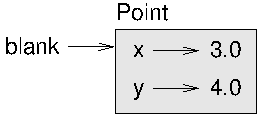
\includegraphics[scale=0.8]{../source/figs/point.pdf}}
\caption{Object diagram.}
\label{fig.point}
\end{figure}

The variable {\tt blank} refers to a Point object, which
contains two attributes.  Each attribute refers to a
floating-point number.

变量 \li{blank} 引用了一个 \li{Point} 类,这个类拥有了两个属性。
每个属性都引用了一个浮点数。

You can read the value of an attribute using the same syntax:

你可以使用相同的语法读取一个属性的值:

\begin{lstlisting}
>>> blank.y
4.0
>>> x = blank.x
>>> x
3.0
\end{lstlisting}
%
The expression {\tt blank.x} means, ``Go to the object {\tt blank}
refers to and get the value of {\tt x}.''  In the example, we assign that
value to a variable named {\tt x}.  There is no conflict between
the variable {\tt x} and the attribute {\tt x}.

表达式 \li{blank.x} 的意思是,``前往 \li{blank} 所引用的对象并且获取 \li{x} 的值''。
在这个例子中,我们将获取到的值赋值给了一个叫做 \li{x} 的变量。
变量 \li{x} 和属性 \li{x} 并不会冲突。

You can use dot notation as part of any expression.  For example:

你可以在任何表达式中使用点标记法。 例如:

\begin{lstlisting}
>>> '(%g, %g)' % (blank.x, blank.y)
'(3.0, 4.0)'
>>> distance = math.sqrt(blank.x**2 + blank.y**2)
>>> distance
5.0
\end{lstlisting}

%
You can pass an instance as an argument in the usual way.
For example:

你可以将一个实例作为参数传递。 例如:

\index{instance!as argument}

\begin{lstlisting}
def print_point(p):
    print('(%g, %g)' % (p.x, p.y))
\end{lstlisting}

%
\verb"print_point" takes a point as an argument and displays it in
mathematical notation.  To invoke it, you can pass {\tt blank} as
an argument:

\li{print_point} 接受一个点作为参数,打印出其在数学中的表示方法。
调用它的时候,你可以将 \li{blank} 作为参数传递:

\begin{lstlisting}
>>> print_point(blank)
(3.0, 4.0)
\end{lstlisting}

%
Inside the function, {\tt p} is an alias for {\tt blank}, so if
the function modifies {\tt p}, {\tt blank} changes.
\index{aliasing}

在这个函数内部, \li{p} 是 \li{blank} 的别名,
所以,如果函数修改了 \li{p} , \li{blank} 也会随之改变。

As an exercise, write a function called \verb"distance_between_points"
that takes two Points as arguments and returns the distance between
them.

我们做个联系,编写一个叫做 \li{distance_between_points} 的函数,它接受两个 \li{Point} 作为参数,然后返回这两个点之间的距离。


\section{Rectangles  |  矩形}
\label{rectangles}

Sometimes it is obvious what the attributes of an object should be,
but other times you have to make decisions.  For example, imagine you
are designing a class to represent rectangles.  What attributes would
you use to specify the location and size of a rectangle?  You can
ignore angle; to keep things simple, assume that the rectangle is
either vertical or horizontal.

有时候,一个对象该拥有哪些属性是显而易见的,但有时候你需要好好考虑一番。
比如,你需要设计一个代表矩形的类。
为了描述一个矩形的位置和大小,你需要设计哪些属性呢?
角度是可以忽略的;为了使事情更简单,我们假设矩形是水平或者竖直的。

\index{representation}

There are at least two possibilities:

至少有两种可能的设计:

\begin{itemize}

\item You could specify one corner of the rectangle
(or the center), the width, and the height.

\item You could specify two opposing corners.

\item 你可以指定矩形的一个角(或是中心)、宽度以及长度。

\item 你可以指定对角线上的两个角。

\end{itemize}

At this point it is hard to say whether either is better than
the other, so we'll implement the first one, just as an example.

这个时候还不能够说明哪个方法优于哪个方法。我们先来实现前者。

\index{Rectangle class}  \index{class!Rectangle}

Here is the class definition:

下面是类的定义:

\begin{lstlisting}
class Rectangle:
    """Represents a rectangle.

    attributes: width, height, corner.
    """
\end{lstlisting}
%
The docstring lists the attributes:  {\tt width} and
{\tt height} are numbers; {\tt corner} is a Point object that
specifies the lower-left corner.

文档字符串中列出了属性: \li{width} 和 \li{height} 是数字;
\li{corner} 是一个 \li{Point} 对象,代表左下角的那个点。

To represent a rectangle, you have to instantiate a Rectangle
object and assign values to the attributes:

为了描述一个矩形,你需要实例化一个 \li{Rectangle} 对象,并且为它的属性赋值:

\begin{lstlisting}
box = Rectangle()
box.width = 100.0
box.height = 200.0
box.corner = Point()
box.corner.x = 0.0
box.corner.y = 0.0
\end{lstlisting}
%
The expression {\tt box.corner.x} means,
``Go to the object {\tt box} refers to and select the attribute named
{\tt corner}; then go to that object and select the attribute named
{\tt x}.''

表达式 \li{box.corner.x} 的意思是,
``前往 \li{box} 所引用的对象,找到叫做 \li{corner} 的属性;
然后前往 \li{corner} 所引用的对象,找到叫做 \li{x} 的属性。''

\begin{figure}
\centerline
{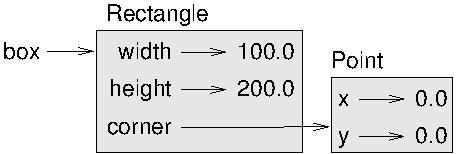
\includegraphics[scale=0.8]{../source/figs/rectangle.pdf}}
\caption{Object diagram.}
\label{fig.rectangle}
\end{figure}

Figure~\ref{fig.rectangle} shows the state of this object.
An object that is an attribute of another object is {\bf embedded}.

图~\ref{fig.rectangle} 展示了这个对象的状态。
一个对象作为另一个对象的属性叫做 {\em 嵌套} (embedded)。
\index{state diagram}  \index{diagram!state}
\index{object diagram}  \index{diagram!object}
\index{embedded object}  \index{object!embedded}


\section{Instances as return values  |  实例作为返回值}
\index{instance!as return value}  \index{return value}

Functions can return instances.  For example, \verb"find_center"
takes a {\tt Rectangle} as an argument and returns a {\tt Point}
that contains the coordinates of the center of the {\tt Rectangle}:

函数可以返回实例。 例如, \li{find_center} 接受一个 \li{Rectangle} 作为参数,
返回一个 \li{Point} ,代表了这个 \li{Rectangle} 的中心坐标:

\begin{lstlisting}
def find_center(rect):
    p = Point()
    p.x = rect.corner.x + rect.width/2
    p.y = rect.corner.y + rect.height/2
    return p
\end{lstlisting}

%
Here is an example that passes {\tt box} as an argument and assigns
the resulting Point to {\tt center}:

下面这个例子将 \li{box} 作为参数传递,然后将返回的 \li{Point} 赋值给 \li{center}:

\begin{lstlisting}
>>> center = find_center(box)
>>> print_point(center)
(50, 100)
\end{lstlisting}
%

\section{Objects are mutable  |  对象是可变的}
\index{object!mutable}  \index{mutability}

You can change the state of an object by making an assignment to one of
its attributes.  For example, to change the size of a rectangle
without changing its position, you can modify the values of {\tt
width} and {\tt height}:


你可以通过给一个对象的属性赋值来改变这个对象的状态。
例如,要改变一个矩形的大小而不改变它的位置,你可以修改 \li{width} 和 \li{height} 的值:

\begin{lstlisting}
box.width = box.width + 50
box.height = box.height + 100
\end{lstlisting}
%
You can also write functions that modify objects.  For example,
\verb"grow_rectangle" takes a Rectangle object and two numbers,
{\tt dwidth} and {\tt dheight}, and adds the numbers to the
width and height of the rectangle:

你也可以编写函数来修改对象。
例如,\li{grow_rectangle} 接受一个\li{Rectangle} 对象和两个数字,
\li{dwidth} 和\li{dheight} ,并将其加到矩形的宽度和高度上:

\begin{lstlisting}
def grow_rectangle(rect, dwidth, dheight):
    rect.width += dwidth
    rect.height += dheight
\end{lstlisting}
%
Here is an example that demonstrates the effect:

下面的例子展示了具体效果:

\begin{lstlisting}
>>> box.width, box.height
(150.0, 300.0)
>>> grow_rectangle(box, 50, 100)
>>> box.width, box.height
(200.0, 400.0)
\end{lstlisting}
%
Inside the function, {\tt rect} is an
alias for {\tt box}, so when the function modifies {\tt rect},
{\tt box} changes.

在函数内部, \li{rect} 是 \li{box} 的一个别名,
所以如果函数修改了 \li{rect} ,则 \li{box} 也随之改变。

As an exercise, write a function named \verb"move_rectangle" that takes
a Rectangle and two numbers named {\tt dx} and {\tt dy}.  It
should change the location of the rectangle by adding {\tt dx}
to the {\tt x} coordinate of {\tt corner} and adding {\tt dy}
to the {\tt y} coordinate of {\tt corner}.

我们做个练习,编写一个叫做 \li{move_rectangle} 的函数,接受一个 \li{Rectangle} 以及两个数字 \li{dx} 和 \li{dy}。  它把 \li{corner} 的 \li{x} 坐标加上 \li{dx},把 \li{corner} 的 \li{y} 坐标加上 \li{dy} ,从而改变矩形的位置。

\section{Copying  |  复制}
\label{copying}
\index{aliasing}

Aliasing can make a program difficult to read because changes
in one place might have unexpected effects in another place.
It is hard to keep track of all the variables that might refer
to a given object.

别名会降低程序的可读性,因为一个地方的变动可能对另一个地方造成预料之外的影响。
跟踪所有引用同一个对象的变量是非常困难的。
\index{copying objects}  \index{object!copying}
\index{copy module}  \index{module!copy}

Copying an object is often an alternative to aliasing.
The {\tt copy} module contains a function called {\tt copy} that
can duplicate any object:

通常用复制对象的方法取代为对象起别名。
\li{copy} 模块拥有一个叫做 \li{copy} 的函数,可以复制任何对象:

\begin{lstlisting}
>>> p1 = Point()
>>> p1.x = 3.0
>>> p1.y = 4.0

>>> import copy
>>> p2 = copy.copy(p1)
\end{lstlisting}

%
{\tt p1} and {\tt p2} contain the same data, but they are
not the same Point.

\li{p1} 和 \li{p2} 拥有相同的数据,但是它们并不是同一个 \li{Point} 对象。

\begin{lstlisting}
>>> print_point(p1)
(3, 4)
>>> print_point(p2)
(3, 4)
>>> p1 is p2
False
>>> p1 == p2
False
\end{lstlisting}

%
The {\tt is} operator indicates that {\tt p1} and {\tt p2} are not the
same object, which is what we expected.  But you might have expected
{\tt ==} to yield {\tt True} because these points contain the same
data.  In that case, you will be disappointed to learn that for
instances, the default behavior of the {\tt ==} operator is the same
as the {\tt is} operator; it checks object identity, not object
equivalence.  That's because for programmer-defined types, Python doesn't
know what should be considered equivalent.  At least, not yet.

正如我们预期的, \li{is} 运算符显示了 \li{p1} 和 \li{p2} 并非同一个对象。
不过你可能会认为 \li{==} 运算的结果应该是 \li{True} ,因为这两个点的数据是相同的。
然而结果并不如你想象的那样, \li{==} 运算符的默认行为和 \li{is} 运算符相同;
它检查对象的标识 (identity) 是否相同,而非对象的值是否相同。  因为 Python 并不知道什么样可以被认为相同。至少目前不知道。
\index{is operator}  \index{operator!is}
\index{identity}  \index{equivalence}

If you use {\tt copy.copy} to duplicate a Rectangle, you will find
that it copies the Rectangle object but not the embedded Point.
\index{embedded object!copying}

如果你使用 \li{copy.copy} 来复制一个 \li{Rectangle} ,
你会发现它仅仅复制了 \li{Rectangle} 对象,但没有复制嵌套的 \li{Point} 对象。

\begin{lstlisting}
>>> box2 = copy.copy(box)
>>> box2 is box
False
>>> box2.corner is box.corner
True
\end{lstlisting}

\begin{figure}
\centerline
{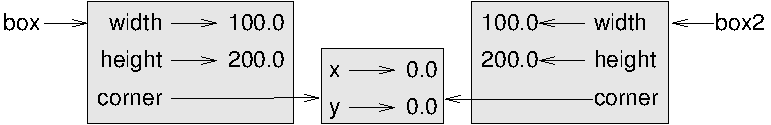
\includegraphics[scale=0.8]{../source/figs/rectangle2.pdf}}
\caption{Object diagram.}
\label{fig.rectangle2}
\end{figure}

Figure~\ref{fig.rectangle2} shows what the object diagram looks like.
\index{state diagram}  \index{diagram!state}
\index{object diagram}  \index{diagram!object}
This operation is called a {\bf shallow copy} because it copies the
object and any references it contains, but not the embedded objects.
\index{shallow copy}  \index{copy!shallow}

图~\ref{fig.rectangle2} 展示了相应的对象图。 这个操作叫做 {\em 浅复制} (shallow
copy) ,因为它仅复制了对象以及其包含的引用, 但未复制嵌套的对象。
\index{state diagram}  \index{diagram!state}
\index{object diagram}  \index{diagram!object}
\index{shallow copy}  \index{copy!shallow}

For most applications, this is not what you want.  In this example,
invoking \verb"grow_rectangle" on one of the Rectangles would not
affect the other, but invoking \verb"move_rectangle" on either would
affect both!  This behavior is confusing and error-prone.

对大多数应用来说,这并非是你想要的结果。
在这个例子中,对其中一个 \li{Rectangle} 对象调用 \li{grow_rectangle}并不会影响到另外一个, 然而当对任何一个 \li{Rectangle} 对象调用 \li{move_rectangle}的时候,两者都会被影响!这个行为很容易带来疑惑和错误。
\index{deep copy}  \index{copy!deep}

Fortunately, the {\tt copy} module provides a method named {\tt
deepcopy} that copies not only the object but also
the objects it refers to, and the objects {\em they} refer to,
and so on.  
You will not be surprised to learn that this operation is
called a {\bf deep copy}.

幸运的是, \li{copy} 模块拥有一个叫做 \li{deepcopy} 的方法,
它不仅可以复制一个对象,还可以复制这个对象所引用的对象,
甚至可以复制 {\bf 这个对象所引用的对象} 所引用的对象,等等。
没错!这个操作叫做 {\em 深复制} (deep copy) 。

\index{deepcopy function}  \index{function!deepcopy}

\begin{lstlisting}
>>> box3 = copy.deepcopy(box)
>>> box3 is box
False
>>> box3.corner is box.corner
False
\end{lstlisting}
%
{\tt box3} and {\tt box} are completely separate objects.

As an exercise, write a version of \verb"move_rectangle" that creates and
returns a new Rectangle instead of modifying the old one.

我们做个练习,编写另一个版本的 \li{move_rectangle} ,
函数创建并返回一个新的 \li{Rectangle} 对象而非修改原先的那个。

\section{Debugging  |  调试}
\label{hasattr}
\index{debugging}

When you start working with objects, you are likely to encounter
some new exceptions.  If you try to access an attribute
that doesn't exist, you get an {\tt AttributeError}:

当你开始学习对象的时候,你可能会遇到一些新的异常。
如果你访问一个不存在的属性,你会得到 \li{Attributeerror} 的错误提示:

\index{exception!AttributeError}  \index{AttributeError}

\begin{lstlisting}
>>> p = Point()
>>> p.x = 3
>>> p.y = 4
>>> p.z
AttributeError: Point instance has no attribute 'z'
\end{lstlisting}

%
If you are not sure what type an object is, you can ask:

如果你不确定一个对象的类型,你可以询问:

\index{type function}  \index{function!type}

\begin{lstlisting}
>>> type(p)
<class '__main__.Point'>
\end{lstlisting}

%
You can also use {\tt isinstance} to check whether an object
is an instance of a class:

你也可以用 \li{isinstance} 来检查某个对象是不是某个类的实例。

\index{isinstance function}  \index{function!isinstance}

\begin{lstlisting}
>>> isinstance(p, Point)
True
\end{lstlisting}

%
If you are not sure whether an object has a particular attribute,
you can use the built-in function {\tt hasattr}:

如果你不确定一个对象是否拥有某个属性, 你可以使用内置函数 \li{hasattr} 检查:
\index{hasattr function}  \index{function!hasattr}

\begin{lstlisting}
>>> hasattr(p, 'x')
True
>>> hasattr(p, 'z')
False
\end{lstlisting}
%
The first argument can be any object; the second argument is a {\em
string} that contains the name of the attribute.

第一个参数可以是任何对象;
第二个参数是一个 {\em 字符串} ,代表了某个属性的名字。

\index{attribute}

You can also use a {\tt try} statement to see if the object has the
attributes you need:

你也可以使用 \li{try} 语句来检查某个对象是不是有你需要的属性:

\index{try statement}  \index{statement!try}

\begin{lstlisting}
try:
    x = p.x
except AttributeError:
    x = 0
\end{lstlisting}

This approach can make it easier to write functions that work with
different types; more on that topic is
coming up in Section~\ref{polymorphism}.

这个方法可以让你更容易编写出可以适应多种数据结构的函数。你可以在 \ref{polymorphism}~节 查看更多内容。


\section{Glossary  |  术语表}

\begin{description}

\item[class:] A programmer-defined type.  A class definition creates a new
class object.

\item[类(class):] 一种程序员自定义的类型。类定义创建了一个新的类对象。
\index{class}  \index{programmer-defined type}  \index{type!programmer-defined}

\item[class object:] An object that contains information about a
programmer-defined type.  The class object can be used to create instances
of the type.

\item[类对象(class object):]包含程序员自定义类型的细节信息的对象。类对象可以被用于创建该类型的实例。

\index{class object}  \index{object!class}

\item[instance:] An object that belongs to a class.

\item[实例(instance):] 属于某个类的对象。
\index{instance}

\item[instantiate:] To create a new object.

\item[实例化(instantiate):] 创建新的对象。
\index{instantiate}

\item[attribute:] One of the named values associated with an object.

\item[属性(attribute):] 和某个对象相关联的有命名的值。
\index{attribute!instance}  \index{instance attribute}

\item[embedded object:] An object that is stored as an attribute
of another object.

\item[嵌套对象(embedded object):] 作为另一个对象的属性存储的对象。
\index{embedded object}  \index{object!embedded}

\item[shallow copy:] To copy the contents of an object, including
any references to embedded objects;
implemented by the {\tt copy} function in the {\tt copy} module.

\item[浅复制(shallow copy):]在复制对象内容的时候,只包含嵌套对象的引用,通过 \li{copy} 模块的 \li{copy} 函数实现。
\index{shallow copy}

\item[deep copy:] To copy the contents of an object as well as any
embedded objects, and any objects embedded in them, and so on;
implemented by the {\tt deepcopy} function in the {\tt copy} module.

\item[深复制(deep copy):]在复制对象内容的时候,既复制对象属性,也复制所有嵌套对象及其中的所有嵌套对象,由 \li{copy} 模块的 \li{deepcopy} 函数实现。
\index{deep copy}

\item[object diagram:] A diagram that shows objects, their
attributes, and the values of the attributes.

\item[对象图(object diagram):] 展示对象及其属性和属性值的图。
\index{object diagram}  \index{diagram!object}

\end{description}


\section{Exercises  |  练习}

\begin{exercise}

Write a definition for a class named {\tt Circle} with attributes
{\tt center} and {\tt radius}, where {\tt center} is a Point object
and radius is a number.

定义一个叫做 \li{Circle} 类,类的属性是圆心( \li{center} ) 和半径( \li{radius} ),其中,圆心( \li{center}) 是一个 \li{Point} 类,而半径( \li{radius})是一个数字。

Instantiate a Circle object that represents a circle with its center
at $(150, 100)$ and radius 75.

实例化一个圆心(center)为 $(150, 100)$ ,半径(radius)为 75 的 $Circle$ 对象。

Write a function named \verb"point_in_circle" that takes a Circle and
a Point and returns True if the Point lies in or on the boundary of
the circle.

编写一个名称为 \li{point_in_circle} 的函数,该函数可以接受一个圆类( \li{Circle})对象和点类 ( \li{Point} )对象,然后判断该点是否在圆内。 在圆内则返回 \li{True} 。

Write a function named \verb"rect_in_circle" that takes a Circle and a
Rectangle and returns True if the Rectangle lies entirely in or on the boundary
of the circle.

编写一个名称为 \li{rect_in_circle} 的函数,该函数接受一个圆类( \li{Circle})对象和矩形( \li{Rectangle})对象,如果该矩形是否完全在圆内或者在圆上则返回 \li{True} 。

Write a function named \verb"rect_circle_overlap" that takes a Circle
and a Rectangle and returns True if any of the corners of the Rectangle fall
inside the circle.  Or as a more challenging version, return True if
any part of the Rectangle falls inside the circle.

编写一个名为 \li{rect_circle_overlap} 函数,该函数接受一个圆类对象和一个矩形类对象,如果矩形有任意一个角落在圆内则返回 \li{True} 。 或者写一个更具有挑战性的版本,如果该矩形有任何部分落在圆内返回 \li{True} 。

Solution: \url{http://thinkpython2.com/code/Circle.py}.

\href{http://thinkpython2.com/code/Circle.py}{参考答案}

\end{exercise}

\begin{exercise}

Write a function called \verb"draw_rect" that takes a Turtle object
and a Rectangle and uses the Turtle to draw the Rectangle.  See
Chapter~\ref{turtlechap} for examples using Turtle objects.

编写一个名为 \li{draw_rect} 的函数,该函数接受一个 \li{Turtle} 对象和一个 \li{Rectangle} 对象,使用 \li{Turtle} 画出该矩形。参考 \ref{turtlechap} 章中使用 \li{Turtle} 的示例。

Write a function called \verb"draw_circle" that takes a Turtle and
a Circle and draws the Circle.

编写一个名为 \li{draw_circle} 的函数,该函数接受一个 \li{Turtle} 对象和 \li{Circle} 对象,并画出该圆。

Solution: \url{http://thinkpython2.com/code/draw.py}.

\href{http://thinkpython2.com/code/draw.py}{参考答案}

\end{exercise}



%🍁% \chapter{Classes and functions}
\chapter{类和函数}
\label{time}

%🍁% Now that we know how to create new types, the next
%🍁% step is to write functions that take programmer-defined objects
%🍁% as parameters and return them as results.  In this chapter I
%🍁% also present ``functional programming style'' and two new
%🍁% program development plans.

现在我们已经知道如何去定义一个新的类型,下一步就是编写以自定义对象为参数的函数,并返回自定义对象作为结果。在本章中,我还将介绍“函数式编程风格”和两种新的编程开发方案。

%🍁% Code examples from this chapter are available from
%🍁% \url{http://thinkpython2.com/code/Time1.py}.
%🍁% Solutions to the exercises are at
%🍁% \url{http://thinkpython2.com/code/Time1_soln.py}.

本章的代码示例可以从 \href{http://thinkpython2.com/code/Time1.py}{这里} 下载。  练习的答案可以从 \href{http://thinkpython2.com/code/Time1_soln.py}{这里} 下载。

%🍁% \section{Time}
\section{时间}
\label{isafter}

%🍁% As another example of a programmer-defined type, we'll define a class
%🍁% called {\tt Time} that records the time of day.  The class definition
%🍁% looks like this: \index{programmer-defined type}

再举一例程序员自定义的类型,我们定义一个叫 \li{Time} 的类,用于记录时间。
这个类将如下定义:
\index{type!programmer-defined} \index{Time class} \index{class!Time}

\begin{lstlisting}
class Time:
    """Represents the time of day.

    attributes: hour, minute, second
    """
\end{lstlisting}

%
%🍁% We can create a new {\tt Time} object and assign
%🍁% attributes for hours, minutes, and seconds:

我们可以创建一个新的 \li{Time} 类对象,并且给它的属性 \li{hour} ,
\li{minutes} 和 \li{seconds} 赋值:

\begin{lstlisting}
time = Time()
time.hour = 11
time.minute = 59
time.second = 30
\end{lstlisting}

%
%🍁% The state diagram for the {\tt Time} object looks like Figure~\ref{fig.time}.

\li{Time} 对象的状态图类似于 图~\ref{fig.time}

\index{state diagram}  \index{diagram!state}
\index{object diagram}  \index{diagram!object}

%🍁% As an exercise, write a function called \verb"print_time" that takes a
%🍁% Time object and prints it in the form {\tt hour:minute:second}.
%🍁% Hint: the format sequence \verb"'%.2d'" prints an integer using
%🍁% at least two digits, including a leading zero if necessary.

我们做个练习,编写一个叫做 \li{print_time} 的函数,
接收一个 \li{Time} 对象并用 \li{时:分:秒} 的格式打印它。
提示:格式化序列 \li{%.2d} 可以至少两位数的形式打印一个整数,如果不足则在前面补0。

%🍁% Write a boolean function called \verb"is_after" that
%🍁% takes two Time objects, {\tt t1} and {\tt t2}, and
%🍁% returns {\tt True} if {\tt t1} follows {\tt t2} chronologically and
%🍁% {\tt False} otherwise.  Challenge: don't use an {\tt if} statement.

编写一个叫做 \li{is_after} 的布尔函数,接收两个 \li{Time}  对象, \li{t1}  和 \li{t2} ,若 \li{t1} 的时间在 \li{t2} 之后,
则返回 \li{True} ,否则返回 \li{False} 。 挑战:不要使用 \li{if} 语句。

\begin{figure}
\centerline
{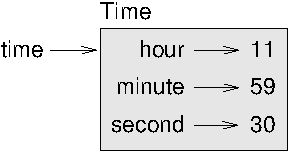
\includegraphics[scale=0.8]{../source/figs/time.pdf}}
\caption{Object diagram.}
\label{fig.time}
\end{figure}

%🍁% \section{Pure functions}
\section{纯函数}
\index{prototype and patch}  \index{development plan!prototype and patch}

%🍁% In the next few sections, we'll write two functions that add time
%🍁% values.  They demonstrate two kinds of functions: pure functions and
%🍁% modifiers.  They also demonstrate a development plan I'll call {\bf
%🍁%   prototype and patch}, which is a way of tackling a complex problem
%🍁% by starting with a simple prototype and incrementally dealing with the
%🍁% complications.
%🍁%
%🍁% Here is a simple prototype of \verb"add_time":

下面几节中,我们将编写两个用来增加时间值的函数。
它们展示了两种不同的函数: {\em 纯函数} (pure functions) 和
{\em 修改器} (modifiers)。
它们也展示了我所称的 {\em 原型和补丁} (prototype and patch) 的开发方案。
这是一种处理复杂问题的方法, 从简单的原型开始, 逐步解决复杂情况。

下面是一个简单的 \li{add_time} 原型:

\begin{lstlisting}
def add_time(t1, t2):
    sum = Time()
    sum.hour = t1.hour + t2.hour
    sum.minute = t1.minute + t2.minute
    sum.second = t1.second + t2.second
    return sum
\end{lstlisting}

%🍁% %
%🍁% The function creates a new {\tt Time} object, initializes its
%🍁% attributes, and returns a reference to the new object.  This is called
%🍁% a {\bf pure function} because it does not modify any of the objects
%🍁% passed to it as arguments and it has no effect,
%🍁% like displaying a value or getting user input,
%🍁% other than returning a value.

这个函数创建了一个新的 \li{Time}
对象,初始化了对象的属性,并返回了这个对象的引用。
我们把这个函数称为 {\em 纯函数} (pure function),
因为它除了返回一个值以外, 并不修改作为参数传入的任何对象,
也没有产生如显示一个值或者获取用户输入的影响。

\index{pure function}  \index{function type!pure}

%🍁% To test this function, I'll create two Time objects: {\tt start}
%🍁% contains the start time of a movie, like {\em Monty Python and the
%🍁% Holy Grail}, and {\tt duration} contains the run time of the movie,
%🍁% which is one hour 35 minutes.

\index{Monty Python and the Holy Grail}

%🍁% \verb"add_time" figures out when the movie will be done.

为了测试这个函数,我将创建两个 \li{Time} 对象: \li{start} 用于存放一个电影
(如 Monty Python and the Holy Grail)的开始时间, \li{duration} 用于存放电影的放映时长,这里时长定为 1 小时 35 分钟。

\li{add_time} 将计算电影何时结束。


\begin{lstlisting}
>>> start = Time()
>>> start.hour = 9
>>> start.minute = 45
>>> start.second =  0

>>> duration = Time()
>>> duration.hour = 1
>>> duration.minute = 35
>>> duration.second = 0

>>> done = add_time(start, duration)
>>> print_time(done)
10:80:00
\end{lstlisting}

%🍁% %
%🍁% The result, {\tt 10:80:00} might not be what you were hoping
%🍁% for.  The problem is that this function does not deal with cases where the
%🍁% number of seconds or minutes adds up to more than sixty.  When that
%🍁% happens, we have to ``carry'' the extra seconds into the minute column
%🍁% or the extra minutes into the hour column.
\index{carrying, addition with}

%🍁% Here's an improved version:

这个结果 \li{10:80:00} 可能不是你所希望得到的。
问题在于这个函数并没有处理好秒数和分钟数相加超过60的情况。
当发生这种情况时,我们要把多余的秒数放进分钟栏,或者把多余的分钟加进小时栏。

下面是一个改进的版本:

\begin{lstlisting}
def add_time(t1, t2):
    sum = Time()
    sum.hour = t1.hour + t2.hour
    sum.minute = t1.minute + t2.minute
    sum.second = t1.second + t2.second

    if sum.second >= 60:
        sum.second -= 60
        sum.minute += 1

    if sum.minute >= 60:
        sum.minute -= 60
        sum.hour += 1

    return sum
\end{lstlisting}

%🍁% %
%🍁% Although this function is correct, it is starting to get big.
%🍁% We will see a shorter alternative later.

这个函数虽然正确,但是它开始变得臃肿。我们会在后面看到一个较短的版本。

\section{Modifiers}
\section{修改器}

\label{increment}
\index{modifier}  \index{function type!modifier}

%🍁% Sometimes it is useful for a function to modify the objects it gets as
%🍁% parameters.  In that case, the changes are visible to the caller.
%🍁% Functions that work this way are called {\bf modifiers}.、

有时候用函数修改作为参数传入的对象是很有用的。在这种情况下,这种改变对
调用者来说是可见的。这种方式工作的函数称为 {\em 修改器} (modifiers)。

\index{increment}

%🍁% {\tt increment}, which adds a given number of seconds to a {\tt Time}
%🍁% object, can be written naturally as a
%🍁% modifier.  Here is a rough draft:

函数 \li{increment} 给一个 \li{Time} 对象增加指定的秒数,
可以很自然地用修改器来编写。  下面是一个原型:

\begin{lstlisting}
def increment(time, seconds):
    time.second += seconds

    if time.second >= 60:
        time.second -= 60
        time.minute += 1

    if time.minute >= 60:
        time.minute -= 60
        time.hour += 1
\end{lstlisting}

%🍁% %
%🍁% The first line performs the basic operation; the remainder deals
%🍁% with the special cases we saw before.

第一行进行基础操作;其余部分的处理则是我们之前看到的特殊情况。

\index{special case}

%🍁% Is this function correct?  What happens if {\tt seconds}
%🍁% is much greater than sixty?

这个函数正确吗? 如果 \li{seconds} 比 60 大很多会发生什么?

%🍁% In that case, it is not enough to carry once; we have to keep doing it
%🍁% until {\tt time.second} is less than sixty.  One solution is to
%🍁% replace the {\tt if} statements with {\tt while} statements.  That
%🍁% would make the function correct, but not very efficient.  As an
%🍁% exercise, write a correct version of {\tt increment} that doesn't
%🍁% contain any loops.

在那种情况下,只进位一次是不够的;我们要重复执行直到 \li{seconds} 小于 60。
一种方法是用 \li{while} 语句代替 \li{if} 语句。
这样能够让函数正确,但是并不是很高效。

%🍁% Anything that can be done with modifiers can also be done with pure
%🍁% functions.  In fact, some programming languages only allow pure
%🍁% functions.  There is some evidence that programs that use pure
%🍁% functions are faster to develop and less error-prone than programs
%🍁% that use modifiers.  But modifiers are convenient at times,
%🍁% and functional programs tend to be less efficient.

任何能够用修改器实现的函数同样能够用纯函数实现。
事实上,一些编程语言只允许用纯函数。
一些证据表明用纯函数实现的程序比用修改器实现的函数开发更快、更不易出错。
但是有时候修改器是很方便的,而函数式程序效率反而不高。

%🍁% In general, I recommend that you write pure functions whenever it is
%🍁% reasonable and resort to modifiers only if there is a compelling
%🍁% advantage.  This approach might be called a {\bf functional
%🍁% programming style}.

通常来说,我推荐只要是合理的情况下,都使用纯函数方式编写,
只在有完全令人信服的原因下采用修改器。
这种方法可以称为 {\em 函数式编程风格} (functional programming style)。

\index{functional programming style}

%🍁% As an exercise, write a ``pure'' version of {\tt increment} that
%🍁% creates and returns a new Time object rather than modifying the
%🍁% parameter.

我们做个练习,编写一个纯函数版本的 \li{increment}  ,
创建并返回一个 \li{Time} 对象,而不是修改参数。


%🍁% \section{Prototyping versus planning}
\section{原型 {\em v.s.} 方案}

\label{prototype}
\index{prototype and patch}  \index{development plan!prototype and patch}
\index{planned development}  \index{development plan!designed}

%🍁% The development plan I am demonstrating is called ``prototype and
%🍁% patch''.  For each function, I wrote a prototype that performed the
%🍁% basic calculation and then tested it, patching errors along the
%🍁% way.

我刚才展示的开发方案叫做 {\em 原型和补丁} (protptype and patch) 。
针对每个函数,我编写了一个可以进行基本运算的原型并对其测试,逐步修正错误。

%🍁% This approach can be effective, especially if you don't yet have a
%🍁% deep understanding of the problem.  But incremental corrections can
%🍁% generate code that is unnecessarily complicated---since it deals with
%🍁% many special cases---and unreliable---since it is hard to know if you
%🍁% have found all the errors.

这种方法在你对问题没有深入理解时特别有效。但增量修正可能导致代码过度复杂,
因为需要处理许多特殊情况。也并不可靠,因为很难知道你是否已经找到了所有的错误。

%🍁% An alternative is {\bf designed development}, in which high-level
%🍁% insight into the problem can make the programming much easier.  In
%🍁% this case, the insight is that a Time object is really a three-digit
%🍁% number in base 60 (see \url{http://en.wikipedia.org/wiki/Sexagesimal}.)!  The
%🍁% {\tt second} attribute is the ``ones column'', the {\tt minute}
%🍁% attribute is the ``sixties column'', and the {\tt hour} attribute is
%🍁% the ``thirty-six hundreds column''.
\index{sexagesimal}

另一种方法叫做 {\em 设计开发} (designed development)。
对问题有高层次的理解能够使开发变得更容易。
这给我们的启示是,\li{Time} 对象本质上是一个基于六十进制的三位数(详见 \href{http://en.wikipedia.org/wiki/Sexagesimal}{此文} 。)!
属性 \li{second} 是``个位'',属性 \li{minute} 是 ``六十位'',属性 \li{hour} 是 ``360位数''。

%🍁% When we wrote \verb"add_time" and {\tt increment}, we were effectively
%🍁% doing addition in base 60, which is why we had to carry from one
%🍁% column to the next.
\index{carrying, addition with}

当我们编写 \li{add_time} 和 \li{increment} 时,其实是在基于六十进制累加,
所以我们需要把一位进位到下一位。

%🍁% This observation suggests another approach to the whole problem---we
%🍁% can convert Time objects to integers and take advantage of the fact
%🍁% that the computer knows how to do integer arithmetic.

这个观察意味着我们可以用另一种方法去解决整个问题——我们可以把
\li{Time} 对象转换为整数,并利用计算机知道如何进行整数运算的这个事实。

%🍁% Here is a function that converts Times to integers:

下面是一个把 \li{Time} 对象转成整数的函数:

\begin{lstlisting}
def time_to_int(time):
    minutes = time.hour * 60 + time.minute
    seconds = minutes * 60 + time.second
    return seconds
\end{lstlisting}

%
%🍁% And here is a function that converts an integer to a Time
%🍁% (recall that {\tt divmod} divides the first argument by the second
%🍁% and returns the quotient and remainder as a tuple).
\index{divmod}

下面则是一个把整数转换为 \li{Time} 对象(回忆一下 \li{divmod} 是用第一个参数除以第二个参数并以元组的形式返回商和余数)。

\begin{lstlisting}
def int_to_time(seconds):
    time = Time()
    minutes, time.second = divmod(seconds, 60)
    time.hour, time.minute = divmod(minutes, 60)
    return time
\end{lstlisting}

%
%🍁% You might have to think a bit, and run some tests, to convince
%🍁% yourself that these functions are correct.  One way to test them is to
%🍁% check that \verb"time_to_int(int_to_time(x)) == x" for many values of
%🍁% {\tt x}.  This is an example of a consistency check.
\index{consistency check}

你可能需要思考一下,并运行一些测试,以此来说服自己这些函数是正确的。
一种测试方法是对很多的 \li{x} 检查 \li{time_to_int(int_to_time(x)) == x}
是否正确。  这是一致性检查的例子。

%🍁% Once you are convinced they are correct, you can use them to
%🍁% rewrite \verb"add_time":

一旦你确信它们是正确的,你就能使用它们重写 \li{add_time} :

\begin{lstlisting}
def add_time(t1, t2):
    seconds = time_to_int(t1) + time_to_int(t2)
    return int_to_time(seconds)
\end{lstlisting}

%
%🍁% This version is shorter than the original, and easier to verify.  As
%🍁% an exercise, rewrite {\tt increment} using \verb"time_to_int" and
%🍁% \verb"int_to_time".

这个版本比先前的要更短,更容易校验。
我们再做个练习,使用 \li{time_to_int} 和 \li{int_to_time}
重写 \li{increment} 函数。

%🍁% In some ways, converting from base 60 to base 10 and back is harder
%🍁% than just dealing with times.  Base conversion is more abstract; our
%🍁% intuition for dealing with time values is better.

从某个方面来说,六十进制和十进制相互转换比处理时间更难些。 进制转换更加抽象;
我们解决时间值的想法是更好的。

%🍁% But if we have the insight to treat times as base 60 numbers and make
%🍁% the investment of writing the conversion functions (\verb"time_to_int"
%🍁% and \verb"int_to_time"), we get a program that is shorter, easier to
%🍁% read and debug, and more reliable.

但如果我们意识到把时间当作六十进制,并预先做好编写转换函数 ( \li{time_to_int}
和 \li{int_to_time}) 的准备,我们就能获得一个更短、更易读、更可靠的程序。

%🍁% It is also easier to add features later.  For example, imagine
%🍁% subtracting two Times to find the duration between them.  The
%🍁% naive approach would be to implement subtraction with borrowing.
%🍁% Using the conversion functions would be easier and more likely to be
%🍁% correct.

这让我们日后更加容易添加其它功能。 例如,试想将两个 \li{Time}
对象相减来获得它们之间的时间间隔。
最简单的方法是使用借位来实现减法。 使用转换函数则更容易,也更容易正确。

\index{subtraction with borrowing}  \index{borrowing, subtraction with}
\index{generalization}

%🍁% Ironically, sometimes making a problem harder (or more general) makes it
%🍁% easier (because there are fewer special cases and fewer opportunities
%🍁% for error).

讽刺的是,有时候把一个问题变得更难(或更加普遍)反而能让它更加简单
(因为会有更少的特殊情况和更少出错的机会)。

%🍁% \section{Debugging}
\section{调试}
\index{debugging}

%🍁% A Time object is well-formed if the values of {\tt minute} and {\tt
%🍁% second} are between 0 and 60 (including 0 but not 60) and if
%🍁% {\tt hour} is positive.  {\tt hour} and {\tt minute} should be
%🍁% integral values, but we might allow {\tt second} to have a
%🍁% fraction part.
\index{invariant}

如果 \li{minute} 和 \li{second} 的值介于 0 和 60 之间
(包括 0 但不包括 60 ),并且 \li{hour} 是正值, 那么这个 \li{Time}
对象就是合法的。 \li{hour} 和 \li{minute} 应该是整数值,
但我们可能也允许  \li{second} 有小数部分。

%🍁% Requirements like these are called {\bf invariants} because
%🍁% they should always be true.  To put it a different way, if they
%🍁% are not true, something has gone wrong.

这样的要求称为 {\em 不变式} (invariants)。 因为它们应当总是为真。
换句话说,如果它们不为真,肯定是某些地方出错了。

%🍁% Writing code to check invariants can help detect errors
%🍁% and find their causes.  For example, you might have a function
%🍁% like \verb"valid_time" that takes a Time object and returns
%🍁% {\tt False} if it violates an invariant:

编写代码来检查不变式能够帮助检测错误并找到出错的原因。
例如,你可能会写一个 \li{valid_time} 这样的函数,
接受一个 \li{Time} 对象,并在违反不变式的条件下返回 \li{False} :

\begin{lstlisting}
def valid_time(time):
    if time.hour < 0 or time.minute < 0 or time.second < 0:
        return False
    if time.minute >= 60 or time.second >= 60:
        return False
    return True
\end{lstlisting}

%
%🍁% At the beginning of each function you could check the
%🍁% arguments to make sure they are valid:

在每个函数的开头,你可以检查参数,确认它们是否合法:

\index{raise statement}  \index{statement!raise}

\begin{lstlisting}
def add_time(t1, t2):
    if not valid_time(t1) or not valid_time(t2):
        raise ValueError('invalid Time object in add_time')
    seconds = time_to_int(t1) + time_to_int(t2)
    return int_to_time(seconds)
\end{lstlisting}

%
%🍁% Or you could use an {\bf assert statement}, which checks a given invariant
%🍁% and raises an exception if it fails:
\index{assert statement}  \index{statement!assert}

或者你可以使用 **assert语句**,检查一个给定的不变式并在失败的情况下抛出异常:

\begin{lstlisting}
def add_time(t1, t2):
    assert valid_time(t1) and valid_time(t2)
    seconds = time_to_int(t1) + time_to_int(t2)
    return int_to_time(seconds)
\end{lstlisting}

%
%🍁% {\tt assert} statements are useful because they distinguish
%🍁% code that deals with normal conditions from code
%🍁% that checks for errors.

\li{assert} 语句非常有用,因为它们区分了处理普通条件的代码和检查错误的代码。

%🍁% \section{Glossary}
\section{术语表}

%🍁% \begin{description}
%🍁%
%🍁% \item[prototype and patch:] A development plan that involves
%🍁% writing a rough draft of a program, testing, and correcting errors as
%🍁% they are found.
%🍁% \index{prototype and patch}
%🍁%
%🍁% \item[designed development:] A development plan that involves
%🍁% high-level insight into the problem and more planning than incremental
%🍁% development or prototype development.
%🍁% \index{designed development}
%🍁%
%🍁% \item[pure function:] A function that does not modify any of the objects it
%🍁% receives as arguments.  Most pure functions are fruitful.
%🍁% \index{pure function}
%🍁%
%🍁% \item[modifier:] A function that changes one or more of the objects it
%🍁%   receives as arguments.  Most modifiers are void; that is, they
%🍁%   return {\tt None}.  \index{modifier}
%🍁%
%🍁% \item[functional programming style:] A style of program design in which the
%🍁% majority of functions are pure.
%🍁% \index{functional programming style}
%🍁%
%🍁% \item[invariant:] A condition that should always be true during the
%🍁% execution of a program.
%🍁% \index{invariant}
%🍁%
%🍁% \item[assert statement:] A statement that check a condition and raises
%🍁% an exception if it fails.
%🍁% \index{assert statement}
%🍁% \index{statement!assert}
%🍁%
%🍁% \end{description}

\begin{description}

\item[原型和补丁 (prototype and patch):]
一种开发方案,编写一个程序的初稿,测试,发现错误时修正它们。
\index{prototype and patch}

\item[设计开发 (designed development):]
一种开发方案,需要对问题有更高层次的理解,比增量开发或原型开发更有计划性。
\index{designed development}

\item[纯函数 (pure function):] 一种不修改任何作为参数传入的对象的函数。大部分纯函数是有返回值的(fruitful)。
\index{pure function}

\item[修改器 (modifier):]
一种修改一个或多个作为参数传入的对象的函数。
大部分修改器没有返回值;即返回 \li{None}
\index{modifier}

\item[函数式编程风格 (functional programming style):]
一种程序设计风格,大部分函数为纯函数。
\index{functional programming style}

\item[不变式 (invariant):]
在程序执行过程中总是为真的条件。
\index{invariant}

\item[(assert statement):]
一种检查条件是否满足并在失败的情况下抛出异常的语句。
\index{assert statement}  \index{statement!assert}

\end{description}

%🍁% \section{Exercises}
\section{练习}
%🍁% Code examples from this chapter are available from
%🍁% \url{http://thinkpython2.com/code/Time1.py}; solutions to the
%🍁% exercises are available from \url{http://thinkpython2.com/code/Time1_soln.py}.

本章的代码示例可以在 \href{http://thinkpython2.com/code/Time1.py}{此处}下载;
练习的答案可以在 \href{http://thinkpython2.com/code/Time1_soln.py}{此处}下载。

\begin{exercise}

%🍁% Write a function called \verb"mul_time" that takes a Time object
%🍁% and a number and returns a new Time object that contains
%🍁% the product of the original Time and the number.
%🍁%
%🍁% Then use \verb"mul_time" to write a function that takes a Time
%🍁% object that represents the finishing time in a race, and a number
%🍁% that represents the distance, and returns a Time object that represents
%🍁% the average pace (time per mile).
%🍁% \index{running pace}

编写一个叫做 \li{mul_time} 的函数,接收一个 \li{Time} 对象和一个数,并返回一个新的 \li{Time} 对象,包含原始时间和数的乘积。

然后使用 \li{mul_time} 编写一个函数,接受一个表示比赛完赛时间的 \li{Time} 对象以及一个表示距离的数字,并返回一个用于表示平均配速(每英里所需时间)的 \li{Time} 对象。

\index{running pace}

\end{exercise}


\begin{exercise}
\index{datetime module}  \index{module!datetime}

%🍁% The {\tt datetime} module provides {\tt time} objects
%🍁% that are similar to the Time objects in this chapter, but
%🍁% they provide a rich set of methods and operators.  Read the
%🍁% documentation at \url{http://docs.python.org/3/library/datetime.html}.
%🍁%
%🍁% \begin{enumerate}
%🍁%
%🍁% \item Use the {\tt datetime} module to write a program that gets the
%🍁%   current date and prints the day of the week.
%🍁%
%🍁% \item Write a program that takes a birthday as input and prints the
%🍁%   user's age and the number of days, hours, minutes and seconds until
%🍁%   their next birthday.
%🍁% \index{birthday}
%🍁%
%🍁% \item For two people born on different days, there is a day when one
%🍁%   is twice as old as the other.  That's their Double Day.  Write a
%🍁%   program that takes two birthdays and computes their Double Day.
%🍁%
%🍁% \item For a little more challenge, write the more general version that
%🍁%   computes the day when one person is $n$ times older than the other.
%🍁% \index{Double Day}
%🍁%
%🍁% \end{enumerate}
%🍁%
%🍁% Solution: \url{http://thinkpython2.com/code/double.py}


\li{datetime} 模块提供的 \li{time} 对象,
和本章的 \li{Time} 对象类似, 但前者提供了更丰富的方法和操作符。
参考阅读 \href{http://docs.python.org/3/library/datetime.html}{相关文档}。

\begin{enumerate}

\item 使用 \li{datetime} 模块来编写一个程序,获取当前日期并打印当天是周几。

\item 编写一个程序,接受一个生日作为输入,并打印用户的年龄以及距离下个生日所需要的天数、小时数、分钟数和秒数。

\item 对于两个不在同一天出生的人来说,总有一天,一个人的出生天数是另一个人的两倍。
   我们把这一天称为 ``双倍日''。  编写一个程序,接受两个不同的出生日期,并计算他们的 ``双倍日''。

\item 再增加点挑战,编写一个更通用的版本,用于计算一个人出生天数是另一个人 $n$ 倍的日子。

\end{enumerate}

\href{http://thinkpython2.com/code/double.py}{参考答案}

\end{exercise}



%🍁% \chapter{Classes and methods}
\chapter{类和方法}

%🍁% Although we are using some of Python's object-oriented features,
%🍁% the programs from the last two chapters are not really
%🍁% object-oriented because they don't represent the relationships
%🍁% between programmer-defined types and the functions that operate
%🍁% on them.  The next step is to transform those functions into
%🍁% methods that make the relationships explicit.

虽然我们已经在使用部分 Python 向对象的特性,
前两个章节中的程序并不是真正面向对象的,
因为它们没有呈现出程序员自定义类型与对其进行操作的函数 (functions) 之间的关系。
下一步,我们将会把这些函数转换成明显突出这一关系的方法 (methods)。


%🍁% Code examples from this chapter are available from
%🍁% \url{http://thinkpython2.com/code/Time2.py}, and solutions
%🍁% to the exercises are in \url{http://thinkpython2.com/code/Point2_soln.py}.

本章代码可以从 \href{http://thinkpython2.com/code/Time2.py}{这里} 获取,
练习题的答案位于\href{http://thinkpython2.com/code/Point2_soln.py}{此处} 。


%🍁% \section{Object-oriented features}
\section{面向对象的特性}
\index{object-oriented programming}  \index{面向对象编程}

%🍁% Python is an {\bf object-oriented programming language}, which means
%🍁% that it provides features that support object-oriented
%🍁% programming, which has these defining characteristics:

Python 是一门 {\em 面向对象的编程语言},
这意味它提供了能够支持面向对象编程的特性。
面向对象编程具有以下特征:

%🍁% \begin{itemize}
%🍁%
%🍁% \item Programs include class and method definitions.
%🍁%
%🍁% \item Most of the computation is expressed in terms of operations on
%🍁%   objects.
%🍁%
%🍁% \item Objects often represent things
%🍁% in the real world, and methods often
%🍁% correspond to the ways things in the real world interact.
%🍁%
%🍁% \end{itemize}

\begin{itemize}

\item 程序包含类和方法定义。

\item 大部分计算以对象上的操作表示。

\item 对象通常代表现实世界的物体,方法对应现实世界中物体交互的方式。

\end{itemize}

%🍁% For example, the {\tt Time} class defined in Chapter~\ref{time}
%🍁% corresponds to the way people record the time of day, and the
%🍁% functions we defined correspond to the kinds of things people do with
%🍁% times.  Similarly, the {\tt Point} and {\tt Rectangle} classes
%🍁% in Chapter~\ref{clobjects}
%🍁% correspond to the mathematical concepts of a point and a rectangle.

例如,第~\ref{time}章中定义的 \li{Time} 类对应人们用来记录一天中的时间,其中定义的各种函数对应人们使用时间的方式。
类似的,第~\ref{clobjects}章中的 \li{Point} 类和 \li{Rectangle} 类对应数学中点和矩形的概念。

%🍁% So far, we have not taken advantage of the features Python provides to
%🍁% support object-oriented programming.  These
%🍁% features are not strictly necessary; most of them provide
%🍁% alternative syntax for things we have already done.  But in many cases,
%🍁% the alternative is more concise and more accurately conveys the
%🍁% structure of the program.

到目前为止,我们还没有利用Python提供的支持面向对象编程的特性。
这些特性严格来说并不是必须的;大部分提供的是我们已经实现的功能的替代语法。
但在很多情况下,这些替代语法更加简洁,更准确地表达了程序的结构。

%🍁% For example, in {\tt Time1.py} there is no obvious
%🍁% connection between the class definition and the function definitions
%🍁% that follow.  With some examination, it is apparent that every function
%🍁% takes at least one {\tt Time} object as an argument.
%🍁% \index{method}
%🍁% \index{function}

例如,在 \li{Time1.py} 中,类定义与之后的函数定义之间没有明显的联系。
仔细检查之后,才会发现每个函数都至少接受一个 \li{Time} 对象作为参数。

%🍁% This observation is the motivation for {\bf methods}; a method is
%🍁% a function that is associated with a particular class.
%🍁% We have seen methods for strings, lists, dictionaries and tuples.
%🍁% In this chapter, we will define methods for programmer-defined types.

从这个观察中我们发现了 {\em 方法} ; 方法是一个与特定的类相关联的函数。
我们已经接触了字符串、列表、字典和元组的方法。
在这章中,我们将会定义程序员自定义类型的方法。

\index{syntax}
\index{semantics}
\index{programmer-defined type}
\index{type!programmer-defined}

%🍁% Methods are semantically the same as functions, but there are
%🍁% two syntactic differences:

方法和函数的语义相同,但是有两处句法的不同:

%🍁% \begin{itemize}
%🍁%
%🍁% \item Methods are defined inside a class definition in order
%🍁% to make the relationship between the class and the method explicit.
%🍁%
%🍁% \item The syntax for invoking a method is different from the
%🍁% syntax for calling a function.
%🍁%
%🍁% \end{itemize}

\begin{itemize}

\item 方法在一个类定义内部声明,为的是显示地与类进行关联。

\item 调用方法的语法和调用函数的语法不同。

\end{itemize}

%🍁% In the next few sections, we will take the functions from the previous
%🍁% two chapters and transform them into methods.  This transformation is
%🍁% purely mechanical; you can do it by following a sequence of
%🍁% steps.  If you are comfortable converting from one form to another,
%🍁% you will be able to choose the best form for whatever you are doing.

在接下来的几节中, 我们会把前面两章中的函数转化为方法。
这个转化是纯机械式的; 你可以通过一系列步骤完成。
如果你能够轻松地将一种形式转换成另一种形式, 就可以选择最适合目前需求的形式。

%🍁% \section{Printing objects}
\section{打印对象 }
\index{object!printing}

%🍁% In Chapter~\ref{time}, we defined a class named
%🍁% {\tt Time} and in Section~\ref{isafter}, you
%🍁% wrote a function named \verb"print_time":

\begin{lstlisting}
class Time:
    """Represents the time of day."""

def print_time(time):
    print('%.2d:%.2d:%.2d' % (time.hour, time.minute, time.second))
\end{lstlisting}

%🍁% %
%🍁% To call this function, you have to pass a {\tt Time} object as an
%🍁% argument:

\begin{lstlisting}
>>> start = Time()
>>> start.hour = 9
>>> start.minute = 45
>>> start.second = 00
>>> print_time(start)
09:45:00
\end{lstlisting}

%🍁% %
%🍁% To make \verb"print_time" a method, all we have to do is
%🍁% move the function definition inside the class definition.  Notice
%🍁% the change in indentation.
\index{indentation}

\begin{lstlisting}
class Time:
    def print_time(time):
        print('%.2d:%.2d:%.2d' % (time.hour, time.minute, time.second))
\end{lstlisting}

%🍁% %
%🍁% Now there are two ways to call \verb"print_time".  The first
%🍁% (and less common) way is to use function syntax:
\index{function syntax}
\index{dot notation}

\begin{lstlisting}
>>> Time.print_time(start)
09:45:00
\end{lstlisting}

%🍁% %
%🍁% In this use of dot notation, {\tt Time} is the name of the class,
%🍁% and \verb"print_time" is the name of the method.  {\tt start} is
%🍁% passed as a parameter.

%🍁% The second (and more concise) way is to use method syntax:
\index{method syntax}

\begin{lstlisting}
>>> start.print_time()
09:45:00
\end{lstlisting}

%🍁% %
%🍁% In this use of dot notation, \verb"print_time" is the name of the
%🍁% method (again), and {\tt start} is the object the method is
%🍁% invoked on, which is called the {\bf subject}.  Just as the
%🍁% subject of a sentence is what the sentence is about, the subject
%🍁% of a method invocation is what the method is about.
\index{subject}

%🍁% Inside the method, the subject is assigned to the first
%🍁% parameter, so in this case {\tt start} is assigned
%🍁% to {\tt time}.
\index{self (parameter name)}
\index{parameter!self}

By convention, the first parameter of a method is
called {\tt self}, so it would be more common to write
\verb"print_time" like this:

\begin{lstlisting}
class Time:
    def print_time(self):
        print('%.2d:%.2d:%.2d' % (self.hour, self.minute, self.second))
\end{lstlisting}

%
The reason for this convention is an implicit metaphor:
\index{metaphor, method invocation}

\begin{itemize}

\item The syntax for a function call, \verb"print_time(start)",
  suggests that the function is the active agent.  It says something
  like, ``Hey \verb"print_time"!  Here's an object for you to print.''

\item In object-oriented programming, the objects are the active
  agents.  A method invocation like \verb"start.print_time()" says
  ``Hey {\tt start}!  Please print yourself.''

\end{itemize}

%🍁% This change in perspective might be more polite, but it is not obvious
%🍁% that it is useful.  In the examples we have seen so far, it may not
%🍁% be.  But sometimes shifting responsibility from the functions onto the
%🍁% objects makes it possible to write more versatile functions (or
%🍁% methods), and makes it easier to maintain and reuse code.
%🍁%
%🍁% As an exercise, rewrite \verb"time_to_int" (from
%🍁% Section~\ref{prototype}) as a method.  You might be tempted to
%🍁% rewrite \verb"int_to_time" as a method, too, but that doesn't
%🍁% really make sense because there would be no object to invoke
%🍁% it on.


%🍁% \section{Another example}
\section{Another example}
\index{increment}

Here's a version of {\tt increment} (from Section~\ref{increment})
rewritten as a method:

\begin{lstlisting}
# inside class Time:

    def increment(self, seconds):
        seconds += self.time_to_int()
        return int_to_time(seconds)
\end{lstlisting}

%
This version assumes that \verb"time_to_int" is written
as a method.  Also, note that
it is a pure function, not a modifier.

Here's how you would invoke {\tt increment}:

\begin{lstlisting}
>>> start.print_time()
09:45:00
>>> end = start.increment(1337)
>>> end.print_time()
10:07:17
\end{lstlisting}

%
The subject, {\tt start}, gets assigned to the first parameter,
{\tt self}.  The argument, {\tt 1337}, gets assigned to the
second parameter, {\tt seconds}.

This mechanism can be confusing, especially if you make an error.
For example, if you invoke {\tt increment} with two arguments, you
get:
\index{exception!TypeError}
\index{TypeError}

\begin{lstlisting}
>>> end = start.increment(1337, 460)
TypeError: increment() takes 2 positional arguments but 3 were given
\end{lstlisting}

%
The error message is initially confusing, because there are
only two arguments in parentheses.  But the subject is also
considered an argument, so all together that's three.

By the way, a {\bf positional argument} is an argument that
doesn't have a parameter name; that is, it is not a keyword
argument.  In this function call:
\index{positional argument}
\index{argument!positional}

\begin{lstlisting}
sketch(parrot, cage, dead=True)
\end{lstlisting}

{\tt parrot} and {\tt cage} are positional, and {\tt dead} is
a keyword argument.


%🍁% \section{A more complicated example}
\section{A more complicated example}

Rewriting \verb"is_after" (from Section~\ref{isafter}) is slightly
more complicated because it takes two Time objects as parameters.  In
this case it is conventional to name the first parameter {\tt self}
and the second parameter {\tt other}: \index{other (parameter name)}
\index{parameter!other}

\begin{lstlisting}
# inside class Time:

    def is_after(self, other):
        return self.time_to_int() > other.time_to_int()
\end{lstlisting}

%
To use this method, you have to invoke it on one object and pass
the other as an argument:

\begin{lstlisting}
>>> end.is_after(start)
True
\end{lstlisting}

%
One nice thing about this syntax is that it almost reads
like English: ``end is after start?''


%🍁% \section{The init method}
\section{The init method}
\index{init method}
\index{method!init}

The init method (short for ``initialization'') is
a special method that gets invoked when an object is instantiated.
Its full name is \verb"__init__" (two underscore characters,
followed by {\tt init}, and then two more underscores).  An
init method for the {\tt Time} class might look like this:

\begin{lstlisting}
# inside class Time:

    def __init__(self, hour=0, minute=0, second=0):
        self.hour = hour
        self.minute = minute
        self.second = second
\end{lstlisting}

%
It is common for the parameters of \verb"__init__"
to have the same names as the attributes.  The statement

\begin{lstlisting}
        self.hour = hour
\end{lstlisting}

%
stores the value of the parameter {\tt hour} as an attribute
of {\tt self}.
\index{optional parameter}
\index{parameter!optional}
\index{default value}
\index{override}

The parameters are optional, so if you call {\tt Time} with
no arguments, you get the default values.

\begin{lstlisting}
>>> time = Time()
>>> time.print_time()
00:00:00
\end{lstlisting}

%
If you provide one argument, it overrides {\tt hour}:

\begin{lstlisting}
>>> time = Time (9)
>>> time.print_time()
09:00:00
\end{lstlisting}

%
If you provide two arguments, they override {\tt hour} and
{\tt minute}.

\begin{lstlisting}
>>> time = Time(9, 45)
>>> time.print_time()
09:45:00
\end{lstlisting}

%
And if you provide three arguments, they override all three
default values.

As an exercise, write an init method for the {\tt Point} class that takes
{\tt x} and {\tt y} as optional parameters and assigns
them to the corresponding attributes.
\index{Point class}
\index{class!Point}


%🍁% \section{The {\tt \_\_str\_\_} method}
\section{The {\tt \_\_str\_\_} method}
\index{str method@\_\_str\_\_ method}
\index{method!\_\_str\_\_}

\verb"__str__" is a special method, like \verb"__init__",
that is supposed to return a string representation of an object.
\index{string representation}

For example, here is a {\tt str} method for Time objects:

\begin{lstlisting}
# inside class Time:

    def __str__(self):
        return '%.2d:%.2d:%.2d' % (self.hour, self.minute, self.second)
\end{lstlisting}

%
When you {\tt print} an object, Python invokes the {\tt str} method:
\index{print statement}
\index{statement!print}

\begin{lstlisting}
>>> time = Time(9, 45)
>>> print(time)
09:45:00
\end{lstlisting}

%
When I write a new class, I almost always start by writing
\verb"__init__", which makes it easier to instantiate objects, and
\verb"__str__", which is useful for debugging.

As an exercise, write a {\tt str} method for the {\tt Point} class.
Create a Point object and print it.


%🍁% \section{Operator overloading}
\section{Operator overloading}
\label{operator.overloading}

By defining other special methods, you can specify the behavior
of operators on programmer-defined types.  For example, if you define
a method named \verb"__add__" for the {\tt Time} class, you can use the
{\tt +} operator on Time objects.
\index{programmer-defined type}
\index{type!programmer-defined}

Here is what the definition might look like:
\index{add method}
\index{method!add}

\begin{lstlisting}
# inside class Time:

    def __add__(self, other):
        seconds = self.time_to_int() + other.time_to_int()
        return int_to_time(seconds)
\end{lstlisting}

%
And here is how you could use it:

\begin{lstlisting}
>>> start = Time(9, 45)
>>> duration = Time(1, 35)
>>> print(start + duration)
11:20:00
\end{lstlisting}

%
When you apply the {\tt +} operator to Time objects, Python invokes
\verb"__add__".  When you print the result, Python invokes
\verb"__str__".  So there is a lot happening behind the scenes!
\index{operator overloading}

Changing the behavior of an operator so that it works with
programmer-defined types is called {\bf operator overloading}.  For every
operator in Python there is a corresponding special method, like
\verb"__add__".  For more details, see
\url{http://docs.python.org/3/reference/datamodel.html#specialnames}.

As an exercise, write an {\tt add} method for the Point class.


%🍁% \section{Type-based dispatch}
\section{Type-based dispatch}

In the previous section we added two Time objects, but you
also might want to add an integer to a Time object.  The
following is a version of \verb"__add__"
that checks the type of {\tt other} and invokes either
\verb"add_time" or {\tt increment}:

\begin{lstlisting}
# inside class Time:

    def __add__(self, other):
        if isinstance(other, Time):
            return self.add_time(other)
        else:
            return self.increment(other)

    def add_time(self, other):
        seconds = self.time_to_int() + other.time_to_int()
        return int_to_time(seconds)

    def increment(self, seconds):
        seconds += self.time_to_int()
        return int_to_time(seconds)
\end{lstlisting}

%
The built-in function {\tt isinstance} takes a value and a
class object, and returns {\tt True} if the value is an instance
of the class.
\index{isinstance function}
\index{function!isinstance}

If {\tt other} is a Time object, \verb"__add__" invokes
\verb"add_time".  Otherwise it assumes that the parameter
is a number and invokes {\tt increment}.  This operation is
called a {\bf type-based dispatch} because it dispatches the
computation to different methods based on the type of the
arguments.
\index{type-based dispatch}
\index{dispatch, type-based}

Here are examples that use the {\tt +} operator with different
types:

\begin{lstlisting}
>>> start = Time(9, 45)
>>> duration = Time(1, 35)
>>> print(start + duration)
11:20:00
>>> print(start + 1337)
10:07:17
\end{lstlisting}

%
Unfortunately, this implementation of addition is not commutative.
If the integer is the first operand, you get
\index{commutativity}

\begin{lstlisting}
>>> print(1337 + start)
TypeError: unsupported operand type(s) for +: 'int' and 'instance'
\end{lstlisting}

%
The problem is, instead of asking the Time object to add an integer,
Python is asking an integer to add a Time object, and it doesn't know
how.  But there is a clever solution for this problem: the
special method \verb"__radd__", which stands for ``right-side add''.
This method is invoked when a Time object appears on the right side of
the {\tt +} operator.  Here's the definition:
\index{radd method}
\index{method!radd}

\begin{lstlisting}
# inside class Time:

    def __radd__(self, other):
        return self.__add__(other)
\end{lstlisting}

%
And here's how it's used:

\begin{lstlisting}
>>> print(1337 + start)
10:07:17
\end{lstlisting}

%

As an exercise, write an {\tt add} method for Points that works with
either a Point object or a tuple:

\begin{itemize}

\item If the second operand is a Point, the method should return a new
Point whose $x$ coordinate is the sum of the $x$ coordinates of the
operands, and likewise for the $y$ coordinates.

\item If the second operand is a tuple, the method should add the
first element of the tuple to the $x$ coordinate and the second
element to the $y$ coordinate, and return a new Point with the result.

\end{itemize}




%🍁% \section{Polymorphism}
\section{Polymorphism}
\label{polymorphism}

Type-based dispatch is useful when it is necessary, but (fortunately)
it is not always necessary.  Often you can avoid it by writing functions
that work correctly for arguments with different types.
\index{type-based dispatch}
\index{dispatch!type-based}

Many of the functions we wrote for strings also
work for other sequence types.
For example, in Section~\ref{histogram}
we used {\tt histogram} to count the number of times each letter
appears in a word.

\begin{lstlisting}
def histogram(s):
    d = dict()
    for c in s:
        if c not in d:
            d[c] = 1
        else:
            d[c] = d[c]+1
    return d
\end{lstlisting}
%
This function also works for lists, tuples, and even dictionaries,
as long as the elements of {\tt s} are hashable, so they can be used
as keys in {\tt d}.

\begin{lstlisting}
>>> t = ['spam', 'egg', 'spam', 'spam', 'bacon', 'spam']
>>> histogram(t)
{'bacon': 1, 'egg': 1, 'spam': 4}
\end{lstlisting}
%
Functions that work with several types are called {\bf polymorphic}.
Polymorphism can facilitate code reuse.  For example, the built-in
function {\tt sum}, which adds the elements of a sequence, works
as long as the elements of the sequence support addition.
\index{polymorphism}

Since Time objects provide an {\tt add} method, they work
with {\tt sum}:

\begin{lstlisting}
>>> t1 = Time(7, 43)
>>> t2 = Time(7, 41)
>>> t3 = Time(7, 37)
>>> total = sum([t1, t2, t3])
>>> print(total)
23:01:00
\end{lstlisting}
%
In general, if all of the operations inside a function
work with a given type, the function works with that type.

The best kind of polymorphism is the unintentional kind, where
you discover that a function you already wrote can be
applied to a type you never planned for.


%🍁% \section{Debugging}
\section{Debugging}
\index{debugging}

It is legal to add attributes to objects at any point in the execution
of a program, but if you have objects with the same type that don't
have the same attributes, it is easy to make mistakes.
It is considered a good idea to
initialize all of an object's attributes in the init method.
\index{init method}
\index{attribute!initializing}

If you are not sure whether an object has a particular attribute, you
can use the built-in function {\tt hasattr} (see Section~\ref{hasattr}).
\index{hasattr function}
\index{function!hasattr}
\index{dict attribute@\_\_dict\_\_ attribute}
\index{attribute!\_\_dict\_\_}

Another way to access attributes is the built-in function {\tt vars},
which takes an object and returns a dictionary that maps from
attribute names (as strings) to their values:

\begin{lstlisting}
>>> p = Point(3, 4)
>>> vars(p)
{'y': 4, 'x': 3}
\end{lstlisting}

%
For purposes of debugging, you might find it useful to keep this
function handy:

\begin{lstlisting}
def print_attributes(obj):
    for attr in vars(obj):
        print(attr, getattr(obj, attr))
\end{lstlisting}

%
\verb"print_attributes" traverses the dictionary
and prints each attribute name and its corresponding value.
\index{traversal!dictionary}
\index{dictionary!traversal}

The built-in function {\tt getattr} takes an object and an attribute
name (as a string) and returns the attribute's value.
\index{getattr function}
\index{function!getattr}


%🍁% \section{Interface and implementation}
\section{Interface and implementation}

One of the goals of object-oriented design is to make software more
maintainable, which means that you can keep the program working when
other parts of the system change, and modify the program to meet new
requirements.
\index{interface}
\index{implementation}
\index{maintainable}
\index{object-oriented design}

A design principle that helps achieve that goal is to keep
interfaces separate from implementations.  For objects, that means
that the methods a class provides should not depend on how the
attributes are represented.
\index{attribute}

For example, in this chapter we developed a class that represents
a time of day.  Methods provided by this class include
\verb"time_to_int", \verb"is_after", and \verb"add_time".

We could implement those methods in several ways.  The details of the
implementation depend on how we represent time.  In this chapter, the
attributes of a {\tt Time} object are {\tt hour}, {\tt minute}, and
{\tt second}.

As an alternative, we could replace these attributes with
a single integer representing the number of seconds
since midnight.  This implementation would make some methods,
like \verb"is_after", easier to write, but it makes other methods
harder.

After you deploy a new class, you might discover a better
implementation.  If other parts of the program are using your
class, it might be time-consuming and error-prone to change the
interface.

But if you designed the interface carefully, you can
change the implementation without changing the interface, which
means that other parts of the program don't have to change.


%🍁% \section{Glossary}
\section{Glossary}

\begin{description}

\item[object-oriented language:] A language that provides features,
  such as programmer-defined types and methods, that facilitate
  object-oriented programming.
\index{object-oriented language}

\item[object-oriented programming:] A style of programming in which
data and the operations that manipulate it are organized into classes
and methods.
\index{object-oriented programming}

\item[method:] A function that is defined inside a class definition and
is invoked on instances of that class.
\index{method}

\item[subject:] The object a method is invoked on.
\index{subject}

\item[positional argument:]  An argument that does not include
a parameter name, so it is not a keyword argument.
\index{positional argument}
\index{argument!positional}

\item[operator overloading:] Changing the behavior of an operator like
{\tt +} so it works with a programmer-defined type.
\index{overloading}
\index{operator!overloading}

\item[type-based dispatch:] A programming pattern that checks the type
of an operand and invokes different functions for different types.
\index{type-based dispatch}

\item[polymorphic:] Pertaining to a function that can work with more
  than one type.
\index{polymorphism}

\item[information hiding:] The principle that the interface provided
by an object should not depend on its implementation, in particular
the representation of its attributes.
\index{information hiding}

\end{description}


%🍁% \section{Exercises}
\section{Exercises}

\begin{exercise}

Download the code from this chapter from
\url{http://thinkpython2.com/code/Time2.py}.  Change the attributes of
    {\tt Time} to be a single integer representing seconds since
    midnight.  Then modify the methods (and the function
    \verb"int_to_time") to work with the new implementation.  You
    should not have to modify the test code in {\tt main}.  When you
    are done, the output should be the same as before.  Solution:
    \url{http://thinkpython2.com/code/Time2_soln.py}.

\end{exercise}


\begin{exercise}
\label{kangaroo}
\index{default value!avoiding mutable}
\index{mutable object, as default value}
\index{worst bug}
\index{bug!worst}
\index{Kangaroo class}
\index{class!Kangaroo}

This exercise is a cautionary tale about one of the most
common, and difficult to find, errors in Python.
Write a definition for a class named {\tt Kangaroo} with the following
methods:

\begin{enumerate}

\item An \verb"__init__" method that initializes an attribute named
\verb"pouch_contents" to an empty list.

\item A method named \verb"put_in_pouch" that takes an object
of any type and adds it to \verb"pouch_contents".

\item A \verb"__str__" method that returns a string representation
of the Kangaroo object and the contents of the pouch.

\end{enumerate}
%
Test your code
by creating two {\tt Kangaroo} objects, assigning them to variables
named {\tt kanga} and {\tt roo}, and then adding {\tt roo} to the
contents of {\tt kanga}'s pouch.

Download \url{http://thinkpython2.com/code/BadKangaroo.py}.  It contains
a solution to the previous problem with one big, nasty bug.
Find and fix the bug.

If you get stuck, you can download
\url{http://thinkpython2.com/code/GoodKangaroo.py}, which explains the
problem and demonstrates a solution.
\index{aliasing}  \index{embedded object}  \index{object!embedded}

\end{exercise}






%🍁% \chapter{Inheritance}
\chapter{继承}

%🍁% The language feature most often associated with object-oriented
%🍁% programming is {\bf inheritance}.  Inheritance is the ability to
%🍁% define a new class that is a modified version of an existing class.
%🍁% In this chapter I demonstrate inheritance using classes that represent
%🍁% playing cards, decks of cards, and poker hands.

最常与面向对象编程联系在一起的语言特性就是 {\em 继承}。  
继承指的是在现有类的基础下进行修改,从而定义新类的能力。  
在本章中,我会用表示卡牌 (playing cards)、一副牌 (deck of hands) 和牌型 (poker hands)的类,来展示继承这一特性。

\index{deck}  \index{card, playing}  \index{poker}

%🍁% If you don't play
%🍁% poker, you can read about it at
%🍁% \url{http://en.wikipedia.org/wiki/Poker}, but you don't have to; I'll
%🍁% tell you what you need to know for the exercises.

如果你不玩扑克牌,你可以 \href{http://en.wikipedia.org/wiki/Poker}{阅读}了解一下,但这不是必须的;我会告诉你完成练习所需要了解的知识点。

%🍁% Code examples from
%🍁% this chapter are available from
%🍁% \url{http://thinkpython2.com/code/Card.py}.

%🍁% \section{Card objects}
\section{卡牌对象}

%🍁% There are fifty-two cards in a deck, each of which belongs to one of
%🍁% four suits and one of thirteen ranks.  The suits are Spades, Hearts,
%🍁% Diamonds, and Clubs (in descending order in bridge).  The ranks are
%🍁% Ace, 2, 3, 4, 5, 6, 7, 8, 9, 10, Jack, Queen, and King.  Depending on
%🍁% the game that you are playing, an Ace may be higher than King
%🍁% or lower than 2.

一副牌有52张牌,每一张属于4种花色的一个和13个等级的一个。  
4种花色是黑桃 (Spades),红心 (Hearts),方块 (Diamonds),梅花 (Clubs),
以桥牌中的逆序排列。  13个等级是A、2、3、4、5、6、7、8、9、10、J、Q、K。  
根据你玩的游戏的不同,A 可能比 K 大或者比 2 小。

\index{rank}  \index{suit}

%🍁% If we want to define a new object to represent a playing card, it is
%🍁% obvious what the attributes should be: {\tt rank} and
%🍁% {\tt suit}.  It is not as obvious what type the attributes
%🍁% should be.  One possibility is to use strings containing words like
%🍁% \verb"'Spade'" for suits and \verb"'Queen'" for ranks.  One problem with
%🍁% this implementation is that it would not be easy to compare cards to
%🍁% see which had a higher rank or suit.

如果我们定义一个新的对象来表示卡牌,明显它应该有 \li{rank} (等级) 和 \li{suit} (花色)
两个属性。  但两个属性的类型不太明显。  一个可能是使用字符串类型,
如 \li{'Spade'} 表示花色,\li{'Queen'} 表示等级。  这种实现的一个问题是,不是那么容易比较牌的大小,看哪张牌的等级或花色更高。

\index{encode}  \index{encrypt}
\index{map to}  \index{representation}

%🍁% An alternative is to use integers to {\bf encode} the ranks and suits.
%🍁% In this context, ``encode'' means that we are going to define a mapping
%🍁% between numbers and suits, or between numbers and ranks.  This
%🍁% kind of encoding is not meant to be a secret (that
%🍁% would be ``encryption'').

另外一种方法,是使用一个整型来 {\em 编码} 等级 和 花色。
在这里,``编码'' 表示我们要定义一个数字到花色或数字到等级的映射。
但是这里的编码并不是为了保密(那就成了``加密'')。

\newcommand{\mymapsto}{$\mapsto$}

%🍁% For example, this table shows the suits and the corresponding integer
%🍁% codes:

例如,下面的表格列出了花色和对应的整数码:

\begin{tabular}{l c l}
Spades & \mymapsto & 3 \\
Hearts & \mymapsto & 2 \\
Diamonds & \mymapsto & 1 \\
Clubs & \mymapsto & 0
\end{tabular}

%🍁% This code makes it easy to compare cards; because higher suits map to
%🍁% higher numbers, we can compare suits by comparing their codes.

整数码使得很容易比较牌的大小;因为更高的花色对应更高的数字,我们可以通过比较数字,来判断花色的的大小。

%🍁% The mapping for ranks is fairly obvious; each of the numerical ranks
%🍁% maps to the corresponding integer, and for face cards:

等级的映射类型选择就显而易见;每个数字等级对应相应的整数,然后对于J,K,Q:

\begin{tabular}{l c l}
Jack & \mymapsto & 11 \\
Queen & \mymapsto & 12 \\
King & \mymapsto & 13 \\
\end{tabular}

%🍁% I am using the \mymapsto~symbol to make it clear that these mappings
%🍁% are not part of the Python program.  They are part of the program
%🍁% design, but they don't appear explicitly in the code.

这里,我使用 \mymapsto~符号来清楚的表示,这些不是 Python 程序的一部分。  它们属于程序设计的一部分,但是不会出现在代码中。

\index{Card class}  \index{class!Card}

%🍁% The class definition for {\tt Card} looks like this:

\li{Card}类的定义如下:

\begin{lstlisting}
class Card:
    """Represents a standard playing card."""

    def __init__(self, suit=0, rank=2):
        self.suit = suit
        self.rank = rank
\end{lstlisting}

%
%🍁% As usual, the init method takes an optional
%🍁% parameter for each attribute.  The default card is
%🍁% the 2 of Clubs.

通常,init 方法接受针对每个属性的可选形参。默认的卡牌是梅花 2。

\index{init method}  \index{method!init}

%🍁% To create a Card, you call {\tt Card} with the
%🍁% suit and rank of the card you want.

可以使用你需要的花色和等级调用 \li{Card} ,创建一个 \li{Card} 对象。

\begin{lstlisting}
queen_of_diamonds = Card(1, 12)
\end{lstlisting}
%

%🍁% \section{Class attributes}
\section{类属性}

\label{class.attribute}
\index{class attribute}  \index{attribute!class}

%🍁% In order to print Card objects in a way that people can easily
%🍁% read, we need a mapping from the integer codes to the corresponding
%🍁% ranks and suits.  A natural way to
%🍁% do that is with lists of strings.  We assign these lists to {\bf class
%🍁% attributes}:

为了以大家能够轻松看懂的方式来打印卡牌对象,我们需要一个从整数码到对应的等级和花色的映射。
一种直接的方法是使用字符串列表。我们把这些列表赋值到 {\em 类属性} :

\begin{lstlisting}
# inside class Card:

    suit_names = ['Clubs', 'Diamonds', 'Hearts', 'Spades']
    rank_names = [None, 'Ace', '2', '3', '4', '5', '6', '7',
              '8', '9', '10', 'Jack', 'Queen', 'King']

    def __str__(self):
        return '%s of %s' % (Card.rank_names[self.rank],
                             Card.suit_names[self.suit])
\end{lstlisting}

%🍁% %
%🍁% Variables like \verb"suit_names" and \verb"rank_names", which are
%🍁% defined inside a class but outside of any method, are called
%🍁% class attributes because they are associated with the class object
%🍁% {\tt Card}.

像 \li{suit_names} 和 \li{rank_names} 这样的变量,是定义在类内部但在方法之外,
被称为类属性。因为他们是被关联到 \li{Card} 类对象上的。

\index{instance attribute}  \index{attribute!instance}

%🍁% This term distinguishes them from variables like {\tt suit} and {\tt
%🍁%   rank}, which are called {\bf instance attributes} because they are
%🍁% associated with a particular instance.
%🍁% \index{dot notation}

这个术语将它们同 \li{suit} 和 \li{rank} 这样的变量区分开来,后者被称为 {\em 实例属性},
因为他们被关联到了特定的实例。

%🍁% Both kinds of attribute are accessed using dot notation.  For
%🍁% example, in \verb"__str__", {\tt self} is a Card object,
%🍁% and {\tt self.rank} is its rank.  Similarly, {\tt Card}
%🍁% is a class object, and \verb"Card.rank_names" is a
%🍁% list of strings associated with the class.

这两种属性都使用点标记法来访问。  
例如,在 \li{__str__} 中, \li{self} 是一个卡牌对象, \li{self.rank} 是它的等级。
同样的, \li{Card} 是一个类对象, \li{Card.rank_names} 是一个和类关联的字符串列表。

%🍁% Every card has its own {\tt suit} and {\tt rank}, but there
%🍁% is only one copy of \verb"suit_names" and \verb"rank_names".

每一张卡牌都有自己的花色和等级,
但是这里只有一份 \li{suit_names} 和 \li{rank_names} 拷贝。

%🍁% Putting it all together, the expression
%🍁% \verb"Card.rank_names[self.rank]" means ``use the attribute {\tt rank}
%🍁% from the object {\tt self} as an index into the list \verb"rank_names"
%🍁% from the class {\tt Card}, and select the appropriate string.''

综合来说,表达式 \li{Card.rank_names[self.rank]} 表示 ``使用 \li{self} 对象
中的 \li{rank} 属性作为 \li{Card} 类的 \li{rank_names} 
列表的索引下标,然后获取相应的字符串。''

%🍁% The first element of \verb"rank_names" is {\tt None} because there
%🍁% is no card with rank zero.  By including {\tt None} as a place-keeper,
%🍁% we get a mapping with the nice property that the index 2 maps to the
%🍁% string \verb"'2'", and so on.  To avoid this tweak, we could have
%🍁% used a dictionary instead of a list.

\li{rank_names} 的第一个元素是 \li{None} ,因为没有卡牌的等级是 0 。
通过使用 \li{None} 作为占位符,我们可以很好地将索引 2 映射到字符串 \li{'2'} ,等等。
为了避免使用这种小技巧,我们也可以使用一个字典来代替列表。

%🍁% With the methods we have so far, we can create and print cards:

利用现有的方法,我们可以创建和打印卡牌:

\begin{lstlisting}
>>> card1 = Card(2, 11)
>>> print(card1)
Jack of Hearts
\end{lstlisting}

\begin{figure}
\centerline
{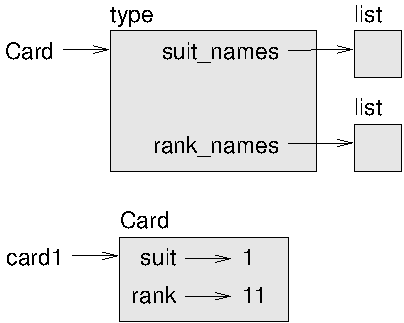
\includegraphics[scale=0.8]{../source/figs/card1.pdf}}
%🍁% \caption{Object diagram.}
\caption{对象图。}
\label{fig.card1}
\end{figure}

%🍁% Figure~\ref{fig.card1} is a diagram of the {\tt Card} class object and
%🍁% one Card instance.  {\tt Card} is a class object; its type is {\tt
%🍁%   type}.  {\tt card1} is an instance of {\tt Card}, so its type is
%🍁% {\tt Card}.  To save space, I didn't draw the contents of
%🍁% \verb"suit_names" and \verb"rank_names".

图~\ref{fig.card1} 是 \li{Card} 类对象和一个 \li{Card} 实例的图示。 \li{Card} 是一个类对象;它的类型是 \li{type} 。 \li{card1} 是 \li{Card} 的一个实例,因此它的类型是 \li{Card}。 为了节省空间,我没有画出 \li{suit_names} 和 \li{rank_names} 的内容。

\index{state diagram}  \index{diagram!state}  
\index{object diagram}  \index{diagram!object}


%🍁% \section{Comparing cards}
\section{卡牌比较}

\label{comparecard}
\index{operator!relational}
\index{relational operator}

%🍁% For built-in types, there are relational operators
%🍁% ({\tt <}, {\tt >}, {\tt ==}, etc.)
%🍁% that compare
%🍁% values and determine when one is greater than, less than, or equal to
%🍁% another.  For programmer-defined types, we can override the behavior of
%🍁% the built-in operators by providing a method named
%🍁% \verb"__lt__", which stands for ``less than''.

对于内建类型,有关系运算符(<, >, ==, 等等)可以比较值,判断哪一个是大于、小于或等于另外一个。
对于程序员自定义的类型,我们可以通过提供一个叫 \li{__lt__} (代表“小于”)的方法,来覆盖内建运算符的行为。

\index{programmer-defined type}
\index{type!programmer-defined}

%🍁% \verb"__lt__" takes two parameters, {\tt self} and {\tt other},
%🍁% and {\tt True} if {\tt self} is strictly less than {\tt other}.

\li{__lt__} 接受 2 个参数, \li{self} 和 \li{other},如果 \li{self} 比 \li{other} 的值要小则返回 \li{True} 。

\index{override}
\index{operator overloading}

%🍁% The correct ordering for cards is not obvious.
%🍁% For example, which
%🍁% is better, the 3 of Clubs or the 2 of Diamonds?  One has a higher
%🍁% rank, but the other has a higher suit.  In order to compare
%🍁% cards, you have to decide whether rank or suit is more important.

卡牌的正确顺序并不明显。  
例如,梅花 3 和方块 2 哪个更高?  
一个等级更高,另一个花色更高。  
为了比较卡牌,你必须决定等级还是花色更重要。  

%🍁% The answer might depend on what game you are playing, but to keep
%🍁% things simple, we'll make the arbitrary choice that suit is more
%🍁% important, so all of the Spades outrank all of the Diamonds,
%🍁% and so on.

答案可能根据你玩的是什么游戏而不同,但是简洁起见,
我们将规定花色更重要,所以所有的黑桃大于任何方块卡牌,以此类推。

\index{cmp method@\_\_cmp\_\_ method}
\index{method!\_\_cmp\_\_}

%🍁% With that decided, we can write \verb"__lt__":

定好了这个规则后,我们可以编写 \li{__lt__} 了:

\begin{lstlisting}
# inside class Card:    
# 在Card类内部:

    def __lt__(self, other):
        # check the suits
        # 判断花色
        if self.suit < other.suit: return True
        if self.suit > other.suit: return False

        # suits are the same... check ranks
        # 花色相同...判断等级
        return self.rank < other.rank
\end{lstlisting}

%🍁% %
%🍁% You can write this more concisely using tuple comparison:

你可以使用元组比较来使得代码更加简洁:

\index{tuple!comparison}
\index{comparison!tuple}

\begin{lstlisting}
# inside class Card:

    def __lt__(self, other):
        t1 = self.suit, self.rank
        t2 = other.suit, other.rank
        return t1 < t2
\end{lstlisting}

%
%🍁% As an exercise, write an \verb"__lt__" method for Time objects.  You
%🍁% can use tuple comparison, but you also might consider
%🍁% comparing integers.

我们做个练习,编写一个 \li{Time} 对象的 \li{__lt__}方法。  
你可以使用元组比较,也可以考虑比较整数。


%🍁% \section{Decks}
\section{一副牌}

\index{list!of objects}
\index{deck, playing cards}

%🍁% Now that we have Cards, the next step is to define Decks.  Since a
%🍁% deck is made up of cards, it is natural for each Deck to contain a
%🍁% list of cards as an attribute.

现在我们有 \li{Card} 类了,下一步是定义完整的一副牌 (Deck)了。  
因为一副牌由许多牌组成,自然地每一个 \li{Deck} 都有一个卡牌列表作为属性。

\index{init method}
\index{method!init}

%🍁% The following is a class definition for {\tt Deck}.  The
%🍁% init method creates the attribute {\tt cards} and generates
%🍁% the standard set of fifty-two cards:

下面是一个 \li{Deck} 的类定义。  
初始化方法创建了 \li{cards} 属性, 然后生成了由 52 张牌组成一副标准卡牌。

\index{composition}  \index{loop!nested}
\index{Deck class}  \index{class!Deck}

\begin{lstlisting}
class Deck:

    def __init__(self):
        self.cards = []
        for suit in range(4):
            for rank in range(1, 14):
                card = Card(suit, rank)
                self.cards.append(card)
\end{lstlisting}

%🍁% %
%🍁% The easiest way to populate the deck is with a nested loop.  The outer
%🍁% loop enumerates the suits from 0 to 3.  The inner loop enumerates the
%🍁% ranks from 1 to 13.  Each iteration
%🍁% creates a new Card with the current suit and rank,
%🍁% and appends it to {\tt self.cards}.

生成一副牌的最简单方法是使用嵌套循环。  
外层循环枚举 0 到 3 的花色。  
内层循环枚举 1 到 13 的等级。  
每一个迭代都用当前的花色和等级创建一张新的牌。  
然后放入 \li{self.cards} 中。

\index{append method}
\index{method!append}


%🍁% \section{Printing the deck}
\section{打印一副牌}

\label{printdeck}
\index{str method@\_\_str\_\_ method}
\index{method!\_\_str\_\_}

%🍁% Here is a \verb"__str__" method for {\tt Deck}:

下面是为 \li{Deck} 定义的 \li{__str__} 方法:

\begin{lstlisting}
#inside class Deck:

    def __str__(self):
        res = []
        for card in self.cards:
            res.append(str(card))
        return '\n'.join(res)
\end{lstlisting}

%
%🍁% This method demonstrates an efficient way to accumulate a large
%🍁% string: building a list of strings and then using the string method
%🍁% {\tt join}.  The built-in function {\tt str} invokes the
%🍁% \verb"__str__" method on each card and returns the string
%🍁% representation.

这个方法展示了累积大字符串的高效方法:建立一个字符串列表然后使用字符串方法 \li{join}。
内建函数 \li{str} 会调用每个卡牌上的 \li{__str__} 方法,并返回它们的字符串表示。

\index{accumulator!string} \index{string!accumulator}
\index{join method} \index{method!join} \index{newline}

%🍁% Since we invoke {\tt join} on a newline character, the cards
%🍁% are separated by newlines.  Here's what the result looks like:

由于我们是在一个换行符上调用的 \li{join} ,卡牌之间被换行符分隔。  下面是结果示例:

\begin{lstlisting}
>>> deck = Deck()
>>> print(deck)
Ace of Clubs
2 of Clubs
3 of Clubs
...
10 of Spades
Jack of Spades
Queen of Spades
King of Spades
\end{lstlisting}

%
%🍁% Even though the result appears on 52 lines, it is
%🍁% one long string that contains newlines.

虽然这个结果有52行,但他实际上是包含换行符的一个长字符串。

%🍁% \section{Add, remove, shuffle and sort}
\section{添加,移除,洗牌和排序}

%🍁% To deal cards, we would like a method that
%🍁% removes a card from the deck and returns it.
%🍁% The list method {\tt pop} provides a convenient way to do that:

为了发牌,我们需要一个可以把卡牌从一副牌中移除并返回的方法。
列表的 \li{pop} 方法提供了一个便捷的实现:

\index{pop method}
\index{method!pop}

\begin{lstlisting}
#inside class Deck:

    def pop_card(self):
        return self.cards.pop()
\end{lstlisting}

%🍁% %
%🍁% Since {\tt pop} removes the {\em last} card in the list, we are
%🍁% dealing from the bottom of the deck.

由于 \li{pop} 移除列表的 {\em 最后一张} 卡牌,所以我们从牌底开始发牌。

\index{append method}
\index{method!append}

%🍁% To add a card, we can use the list method {\tt append}:

\begin{lstlisting}
#inside class Deck:

    def add_card(self, card):
        self.cards.append(card)
\end{lstlisting}

%🍁% %
%🍁% A method like this that uses another method without doing
%🍁% much work is sometimes called a {\bf veneer}.  The metaphor
%🍁% comes from woodworking, where a veneer is a thin
%🍁% layer of good quality wood glued to the surface of a cheaper piece of
%🍁% wood to improve the appearance.

像上面这样利用别的方法 (method),自己却没有做太多处理的方法,
有时候被称为 {\em 伪装方法} (veneer)。  
这个隐喻来源于木工行业, 他们通常用一片高质量的木质薄层粘贴在一块便宜木材的表面,改善外观形象。

\index{veneer}

%🍁% In this case \verb"add_card" is a ``thin'' method that expresses
%🍁% a list operation in terms appropriate for decks.  It
%🍁% improves the appearance, or interface, of the
%🍁% implementation.

在这里,\li{add_card} 是一个“瘦”方法,以卡牌的术语来表述一个列表操作。  
它改善了实现的外观,或者说接口。

%🍁% As another example, we can write a Deck method named {\tt shuffle}
%🍁% using the function {\tt shuffle} from the {\tt random} module:

再举一个例子,我们可以用 \li{random} 模块中的 
\li{shuffle} 函数,给 \li{Deck} 写一个叫 \li{shuffle} 的方法。

\index{random module}
\index{module!random}
\index{shuffle function}
\index{function!shuffle}

\begin{lstlisting}
# inside class Deck:

    def shuffle(self):
        random.shuffle(self.cards)
\end{lstlisting}

%🍁% %
%🍁% Don't forget to import {\tt random}.

不要忘记了导入 \li{random} 。

%🍁% As an exercise, write a Deck method named {\tt sort} that uses the
%🍁% list method {\tt sort} to sort the cards in a {\tt Deck}.  {\tt sort}
%🍁% uses the \verb"__lt__" method we defined to determine the order.

我们做个练习,用列表的 \li{sort} 方法来写一个 \li{Deck} 的 \li{sort} 方法,给卡牌排序。
 \li{sort} 使用我们定义的 \li{__cmp__} 来决定排序顺序。

\index{sort method} \index{method!sort}


%🍁% \section{Inheritance}
\section{继承}

\index{inheritance}
\index{object-oriented programming}

%🍁% Inheritance is the ability to define a new class that is a modified
%🍁% version of an existing class.  As an example, let's say we want a
%🍁% class to represent a ``hand'', that is, the cards held by one player.
%🍁% A hand is similar to a deck: both are made up of a collection of
%🍁% cards, and both require operations like adding and removing cards.

继承指的是在现有类的基础下进行修改,从而定义新类的能力。  
例如,假设我们想定义一个类来代表手牌(hand),即玩家目前手里有的牌。  
手牌与一副牌 (deck)类似:二者都由卡牌组成,都要求支持添加和移除卡牌的操作。

%🍁% A hand is also different from a deck; there are operations we want for
%🍁% hands that don't make sense for a deck.  For example, in poker we
%🍁% might compare two hands to see which one wins.  In bridge, we might
%🍁% compute a score for a hand in order to make a bid.

但二者也有区别;有些我们希望手牌具备的操作,对于 deck 来说并不合理。  
例如,在扑克牌中,我们可能需要比较两个手牌,比较哪方赢了。  
在桥牌中,我们可能需要计算手牌的得分,才好下注。

%🍁% This relationship between classes---similar, but different---lends
%🍁% itself to inheritance.
%🍁% To define a new class that inherits from an existing class,
%🍁% you put the name of the existing class in parentheses:

类之间有相似之处,但也存在不同,这时就可以用上继承了。  
你只需要在定义新类时,将现有类的名称放在括号里,即可继承现有类:

\index{parentheses!parent class in}
\index{parent class}
\index{class!parent}
\index{Hand class}
\index{class!Hand}

\begin{lstlisting}
class Hand(Deck):
    """Represents a hand of playing cards."""
\end{lstlisting}

%🍁% %
%🍁% This definition indicates that {\tt Hand} inherits from {\tt Deck};
%🍁% that means we can use methods like \verb"pop_card" and \verb"add_card"
%🍁% for Hands as well as Decks.

这个定义表明,\li{Hand} 继承自 \li{Deck} ;  这意味着我们也可以对 \li{Hands} 使用 \li{Deck} 的 \li{pop_card} 和 \li{add_card} 方法。

%🍁% When a new class inherits from an existing one, the existing
%🍁% one is called the {\bf parent} and the new class is
%🍁% called the {\bf child}.

当一个新类继承自一个现有类时,现有类被称为 {\em 父类} (parent) ,新类被称为 {\em 子类} (child) 。

\index{parent class}
\index{child class}
\index{class!child}

%🍁% In this example, {\tt Hand} inherits \verb"__init__" from {\tt Deck},
%🍁% but it doesn't really do what we want: instead of populating the hand
%🍁% with 52 new cards, the init method for Hands should initialize {\tt
%🍁%   cards} with an empty list.  \index{override} \index{init method}

在此例中, \li{Hand} 继承了 \li{Deck} 的 \li{__init__} 方法, 
但是它并没有满足我们的要求:init 方法应该为 \li{Hand} 初始化一个空的 \li{cards} 
列表,而不是往手牌里添加 52 张新牌。

\index{method!init}

%🍁% If we provide an init method in the {\tt Hand} class, it overrides the
%🍁% one in the {\tt Deck} class:

如果我们提供一个 \li{Hand} 的 init 方法,它会覆盖从 \li{Deck} 类继承来的同名方法。

\begin{lstlisting}
# inside class Hand:

    def __init__(self, label=''):
        self.cards = []
        self.label = label
\end{lstlisting}

%🍁% %
%🍁% When you create a Hand, Python invokes this init method, not the
%🍁% one in {\tt Deck}.

当你创建一个 \li{Hand} 时,Python 会调用这个 init 方法,而不是 \li{Deck} 中的同名方法。

\begin{lstlisting}
>>> hand = Hand('new hand')
>>> hand.cards
[]
>>> hand.label
'new hand'
\end{lstlisting}

%🍁% %
%🍁% The other methods are inherited from {\tt Deck}, so we can use
%🍁% \verb"pop_card" and \verb"add_card" to deal a card:

其它方法是从 \li{Deck} 继承来的,所以我们可以使用 \li{pop_card} 和 
\li{add_card} 来发牌:

\begin{lstlisting}
>>> deck = Deck()
>>> card = deck.pop_card()
>>> hand.add_card(card)
>>> print(hand)
King of Spades
\end{lstlisting}

%🍁% %
%🍁% A natural next step is to encapsulate this code in a method
%🍁% called \verb"move_cards":

很自然地,下一步就是把这些代码封装进一个叫 \li{move_cards} 的方法:

\index{encapsulation}

\begin{lstlisting}
#inside class Deck:

    def move_cards(self, hand, num):
        for i in range(num):
            hand.add_card(self.pop_card())
\end{lstlisting}

%🍁% %
%🍁% \verb"move_cards" takes two arguments, a Hand object and the number of
%🍁% cards to deal.  It modifies both {\tt self} and {\tt hand}, and
%🍁% returns {\tt None}.

\li{move_cards} 接受两个参数,一个是 \li{Hand} 对象,另一个是发牌的数量。
它会同时修改 \li{self} 和 \li{hand} ,然后返回 \li{None} 。

%🍁% In some games, cards are moved from one hand to another,
%🍁% or from a hand back to the deck.  You can use \verb"move_cards"
%🍁% for any of these operations: {\tt self} can be either a Deck
%🍁% or a Hand, and {\tt hand}, despite the name, can also be a {\tt Deck}.

在有些游戏里面,卡牌从一个手牌移动到另外一个手牌,或者从手牌退还到牌堆里面。
任何这些操作都可以使用 \li{move_cards} : \li{self} 可以是一个 \li{Deck} 或者一个 \li{Hand} ,而且尽管名字叫 \li{hand} ,它也可以是一个 \li{Deck} 。

%🍁% Inheritance is a useful feature.  Some programs that would be
%🍁% repetitive without inheritance can be written more elegantly
%🍁% with it.  Inheritance can facilitate code reuse, since you can
%🍁% customize the behavior of parent classes without having to modify
%🍁% them.  In some cases, the inheritance structure reflects the natural
%🍁% structure of the problem, which makes the design easier to
%🍁% understand.

继承是一个非常有用的特性。有了继承,一些重复性的代码可以写得非常的优雅。
继承有助于代码重用,因为你可以在不修改父类定义的前提下,就改变父类的行为。
在有些情况下,继承的结构反映了真实问题的结构,使得程序更易于理解。

%🍁% On the other hand, inheritance can make programs difficult to read.
%🍁% When a method is invoked, it is sometimes not clear where to find its
%🍁% definition.  The relevant code may be spread across several modules.
%🍁% Also, many of the things that can be done using inheritance can be
%🍁% done as well or better without it.

另一方面,继承又有可能会使得程序更加难读。
当调用一个方法时,有时候搞不清楚去哪找它的定义。
相关的代码可能被分散在几个模块之中。
而且,许多用继承能完成的事情,不用继承也可以完成,有可能还完成得更好。

%🍁% \section{Class diagrams}
\section{类图}
\label{class.diagram}

%🍁% So far we have seen stack diagrams, which show the state of
%🍁% a program, and object diagrams, which show the attributes
%🍁% of an object and their values.  These diagrams represent a snapshot
%🍁% in the execution of a program, so they change as the program
%🍁% runs.

到目前为止我们已经了解过栈图,它显示的是一个程序的状态;  
以及对象图,它显示的是一个对象的属性及其值。  
这些图代表了程序执行中的一个快照,所以它们随着程序的运行而变化。

%🍁% They are also highly detailed; for some purposes, too
%🍁% detailed.  A class diagram is a more abstract representation
%🍁% of the structure of a program.  Instead of showing individual
%🍁% objects, it shows classes and the relationships between them.

它们也十分的详细;但有些时候显得过于详细了。  
类图是程序结构的一种更加抽象的表达。  
它显示的是类和类之间的关系,而不是每个独立的对象。  

%🍁% There are several kinds of relationship between classes:

类之间有如下几种关系:

\begin{itemize}

%🍁% \item Objects in one class might contain references to objects
%🍁% in another class.  For example, each Rectangle contains a reference
%🍁% to a Point, and each Deck contains references to many Cards.
%🍁% This kind of relationship is called {\bf HAS-A}, as in, ``a Rectangle
%🍁% has a Point.''

\item 一个类中的对象可以包含对另外一个类的对象的引用。  
例如,每一个矩形包含对点的引用,每一个 \li{Deck} 包含对许多 \li{Card} 的引用。 这种关系被称为{\em 组合} ({\bf HAS-A}),可以类似这样描述:``一个矩形有一个(has a)点''。

%🍁% \item One class might inherit from another.  This relationship
%🍁% is called {\bf IS-A}, as in, ``a Hand is a kind of a Deck.''

\item 一个类可能继承自另外一个类。  
这种关系被称为 {\em 继承} ({\bf IS-A}), 可以类似这样描述:``Hand is a kind of Deck''。

%🍁% \item One class might depend on another in the sense that objects
%🍁% in one class take objects in the second class as parameters, or
%🍁% use objects in the second class as part of a computation.  This
%🍁% kind of relationship is called a {\bf dependency}.

\item 一个类可能强赖另一个类,因为前者中的对象接受后者中的对象作为参数,
或者使用后者中的对象作为计算的一部分。这种关系被称为 {\em 依赖} ({\bf dependency})。

\end{itemize}

\index{IS-A relationship}
\index{HAS-A relationship}
\index{class diagram}
\index{diagram!class}

%🍁% A {\bf class diagram} is a graphical representation of these
%🍁% relationships.  For example, Figure~\ref{fig.class1} shows the
%🍁% relationships between {\tt Card}, {\tt Deck} and {\tt Hand}.

类图是这些关系的图形化表示。  例如,图~\ref{fig.class1} 标明了 \li{Card} , \li{Deck} 和
\li{Hand} 之间的关系。

\begin{figure}
\centerline
{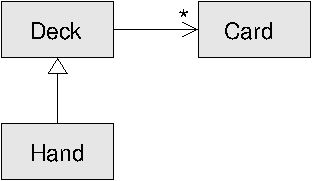
\includegraphics[scale=0.8]{../source/figs/class1.pdf}}
%🍁% \caption{Class diagram.}
\caption{类图。}
\label{fig.class1}
\end{figure}

%🍁% The arrow with a hollow triangle head represents an IS-A
%🍁% relationship; in this case it indicates that Hand inherits
%🍁% from Deck.

带空心三角的箭头表示 IS-A 的关系; 这里它表示 \li{Hand} 继承自 \li{Deck} 。

%🍁% The standard arrow head represents a HAS-A
%🍁% relationship; in this case a Deck has references to Card
%🍁% objects.

标准箭头表示 HAS-A 的关系; 这里表示 \li{Deck} 包含对 \li{Card} 对象的引用。

\index{multiplicity (in class diagram)}

%🍁% The star ({\tt *}) near the arrow head is a
%🍁% {\bf multiplicity}; it indicates how many Cards a Deck has.
%🍁% A multiplicity can be a simple number, like {\tt 52}, a range,
%🍁% like {\tt 5..7} or a star, which indicates that a Deck can
%🍁% have any number of Cards.

箭头旁边的星号是一个复数 ({\bf multiplicity})表达;  
它表示 \li{Deck} 包含多少个 \li{Card}。  
一个复数表达可以是一个简单的数字(如 52 ), 
一个范围(如 \li{5..7} 或者是 \li{*},表示有任意数量的 \li{Card} 。

%🍁% There are no dependencies in this diagram.  They would normally
%🍁% be shown with a dashed arrow.  Or if there are a lot of
%🍁% dependencies, they are sometimes omitted.

图中没有标出依赖关系。  这种关系通常使用虚线箭头表示。  
或者,如果有很多依赖关系的话,有时候会省略。  

%🍁% A more detailed diagram might show that a Deck actually
%🍁% contains a {\em list} of Cards, but built-in types
%🍁% like list and dict are usually not included in class diagrams.

一个更详细的类图可能会显示 \li{Deck} 实际包含了一个由 \li{Cards} 组成的列表,但是通常类图中不会包含 \li{list} 和 \li{dict} 等内建类型。


%🍁% \section{Data encapsulation}
\section{数据封装}

%🍁% The previous chapters demonstrate a development plan we might call
%🍁% ``object-oriented design''.  We identified objects we needed---like
%🍁% {\tt Point}, {\tt Rectangle} and {\tt Time}---and defined classes to
%🍁% represent them.  In each case there is an obvious correspondence
%🍁% between the object and some entity in the real world (or at least a
%🍁% mathematical world).

前面几章中描述了一种可以称为 ``面向对象设计'' 的开发计划。  
我们确定所需要的对象 —— 如 \li{Point}、 \li{Rectangle} 和 \li{Time} —— 然后定义代表它们的类。
对于每个类来说,这个类对象和真实世界(或至少是数学世界)中的某种实体具有明显的对应关系。

\index{development plan!data encapsulation}

%🍁% But sometimes it is less obvious what objects you need
%🍁% and how they should interact.  In that case you need a different
%🍁% development plan.  In the same way that we discovered function
%🍁% interfaces by encapsulation and generalization, we can discover
%🍁% class interfaces by {\bf data encapsulation}.

但是有时有很难界定你需要的对象以及它们如何交互。  
在这个时候, 你需要一个不同的开发计划。  
之前我们通过封装和泛化来编写函数接口, 我们同样可以通过 {\em 数据封装} 来编写类接口。

\index{data encapsulation}

%🍁% Markov analysis, from Section~\ref{markov}, provides a good example.
%🍁% If you download my code from \url{http://thinkpython2.com/code/markov.py},
%🍁% you'll see that it uses two global variables---\verb"suffix_map" and
%🍁% \verb"prefix"---that are read and written from several functions.

\ref{markov}~节 中介绍的马尔科夫分析就是一个很好的例子。  
如果你下载我的\href{http://thinkpython2.com/code/markov.py}{代码}, 你会发现它使用了两个全局变量 —— \li{suffix_map} 和 \li{prefix}, 它们被多个函数进行读写。

\begin{lstlisting}
suffix_map = {}
prefix = ()
\end{lstlisting}

%🍁% Because these variables are global, we can only run one analysis at a
%🍁% time.  If we read two texts, their prefixes and suffixes would be
%🍁% added to the same data structures (which makes for some interesting
%🍁% generated text).

因为这些变量是全局的,我们一次只能运行一个分析。如果我们读取了两个文本,
它们的前缀和后缀会被加入相同的数据结构(会使得输出文本混乱)。

%🍁% To run multiple analyses, and keep them separate, we can encapsulate
%🍁% the state of each analysis in an object.
%🍁% Here's what that looks like:

如果想同时运行多个分析,并且保持它们的相互独立,我们可以把每个分析的状态封装到一个对象中。
下面是一个示例:

\begin{lstlisting}
class Markov:

    def __init__(self):
        self.suffix_map = {}
        self.prefix = ()
\end{lstlisting}

%🍁% Next, we transform the functions into methods.  For example,
%🍁% here's \verb"process_word":

下一步,我们把这些函数转换为方法。  
例如:下面是 \li{process_word} :

\begin{lstlisting}
    def process_word(self, word, order=2):
        if len(self.prefix) < order:
            self.prefix += (word,)
            return

        try:
            self.suffix_map[self.prefix].append(word)
        except KeyError:
            # if there is no entry for this prefix, make one
            self.suffix_map[self.prefix] = [word]

        self.prefix = shift(self.prefix, word)
\end{lstlisting}

%🍁% Transforming a program like this---changing the design without
%🍁% changing the behavior---is another example of refactoring
%🍁% (see Section~\ref{refactoring}).

像这样改变一个程序 --- 改变设计而保持功能不变 --- 是代码重构的另一个例子
(参见\ref{refactoring}~节)。

\index{refactoring}

%🍁% This example suggests a development plan for designing objects and
%🍁% methods:

下面的例子给出了一种设计对象和方法的开发计划:

\begin{enumerate}

%🍁% \item Start by writing functions that read and write global
%🍁% variables (when necessary).
%🍁% 
%🍁% \item Once you get the program working, look for associations
%🍁% between global variables and the functions that use them.
%🍁% 
%🍁% \item Encapsulate related variables as attributes of an object.
%🍁% 
%🍁% \item Transform the associated functions into methods of the new
%🍁% class.

\item 首先编写读取全局变量的函数(如有必要)。

\item 一旦你让程序跑起来了,开始查找全局变量和使用它们的函数的联系。

\item 封装相关的变量作为一个对象的属性。

\item 转换相关函数为新类的方法。

\end{enumerate}

%🍁% As an exercise, download my Markov code from
%🍁% \url{http://thinkpython2.com/code/markov.py}, and follow the steps
%🍁% described above to encapsulate the global variables as attributes of a
%🍁% new class called {\tt Markov}.  Solution:
%🍁% \url{http://thinkpython2.com/code/Markov.py} (note the capital M).

我们做个练习,下载我的\href{http://thinkpython2.com/code/markov.py}{马尔科夫分析代码},然后按照上面所述的步骤,将全局变量封装为新类 \li{Markov} (注意M为大写)的属性。


%🍁% \section{Debugging}
\section{调试}
\index{debugging}

%🍁% Inheritance can make debugging difficult because when you invoke a
%🍁% method on an object, it might be hard to figure out which method will
%🍁% be invoked.

继承会使得调试变得更加复杂,因为你可能不知道实际调用的是哪个类的方法。

\index{inheritance}

%🍁% Suppose you are writing a function that works with Hand objects.
%🍁% You would like it to work with all kinds of Hands, like
%🍁% PokerHands, BridgeHands, etc.  If you invoke a method like
%🍁% {\tt shuffle}, you might get the one defined in {\tt Deck},
%🍁% but if any of the subclasses override this method, you'll
%🍁% get that version instead.  This behavior is usually a good
%🍁% thing, but it can be confusing.

假设你在写一个处理 \li{Hand} 对象的函数。  
你可能会想让它可以处理所有种类的 \li{Hand} ,
如 \li{PockerHands} , \li{BridgeHands} ,等等。  
如果你调用类似 \li{shuffle} 这样的方法,你可能会得到 \li{Deck} 中定义的那个,
但是如果有任何一个子类覆盖了这个方法。你实际上得到的是子类的那个方法。  
这个行为通常是一件好事,但是容易让人混淆。

%🍁% Any time you are unsure about the flow of execution through your
%🍁% program, the simplest solution is to add print statements at the
%🍁% beginning of the relevant methods.  If {\tt Deck.shuffle} prints a
%🍁% message that says something like {\tt Running Deck.shuffle}, then as
%🍁% the program runs it traces the flow of execution.

只要你不确定程序的执行流程,最简单的方法是在相关方法的开始处添加 \li{print} 语
句。  如果 \li{Deck.shuffle} 打印一条如像 \li{Running Deck.shuffle} 的消息,
那么随着程序的运行,它会追踪执行的流程。

\index{flow of execution}

%🍁% As an alternative, you could use this function, which takes an
%🍁% object and a method name (as a string) and returns the class that
%🍁% provides the definition of the method:

另外一种方法是使用下面的函数,它接受一个对象和一个方法的名字(字符串格式)作
为参数,然后返回提供这个方法定义的类:

\begin{lstlisting}
def find_defining_class(obj, meth_name):
    for ty in type(obj).mro():
        if meth_name in ty.__dict__:
            return ty
\end{lstlisting}

%🍁% %
%🍁% Here's an example:
例如:

\begin{lstlisting}
>>> hand = Hand()
>>> find_defining_class(hand, 'shuffle')
<class 'Card.Deck'>
\end{lstlisting}

%🍁% %
%🍁% So the {\tt shuffle} method for this Hand is the one in {\tt Deck}.

所以 \li{Hand} 的 \li{shuffle} 方法是来自于 \li{Deck} 的。

\index{mro method}
\index{method!mro}
\index{method resolution order}

%🍁% \verb"find_defining_class" uses the {\tt mro} method to get the list
%🍁% of class objects (types) that will be searched for methods.  ``MRO''
%🍁% stands for ``method resolution order'', which is the sequence of
%🍁% classes Python searches to ``resolve'' a method name.

\li{find_defining_class} 使用 \li{mro} 方法获得将类对象(类型)的列表,
解释器将会从这里依次搜索哪个类提供了这个方法。  
``MOR'' 是 ``method resolution order''的简称, 指的是Python ``解析'' 方法名时将搜索的一个类序列。

%🍁% Here's a design suggestion: when you override a method,
%🍁% the interface of the new method should be the same as the old.  It
%🍁% should take the same parameters, return the same type, and obey the
%🍁% same preconditions and postconditions.  If you follow this rule, you
%🍁% will find that any function designed to work with an instance of a
%🍁% parent class, like a Deck, will also work with instances of child
%🍁% classes like a Hand and PokerHand.


我提一个对程序设计的建议:当你覆盖一个方法时,新方法的接口应该与旧方法保持一致。
它们应该接受相同的参数,返回相同的类型,遵守相同的先决条件和后置条件。
如果你遵循这个原则,你会发现:任何你设计的函数,只要能用于一个父类的对象(
如 \li{Deck} ),就能够用于任何子类的实例(如 \li{Hand} 和 \li{PockerHand} )。

\index{override}
\index{interface}
\index{precondition}
\index{postcondition}

%🍁% If you violate this rule, which is called the ``Liskov substitution
%🍁% principle'', your code will collapse like (sorry) a house of cards.

如果你违背这条规则(该原则被称为``里氏代换原理'',Liskov substitution
principle),你的代码逻辑就会变得乱七八糟。

\index{Liskov substitution principle}

%🍁% \section{Glossary}
\section{术语表}

\begin{description}

%🍁% \item[encode:]  To represent one set of values using another
%🍁% set of values by constructing a mapping between them.

\item[编码 (encode)]  利用另一组值代表一组值,方法时构建二者之间的映射。
\index{encode}

%🍁% \item[class attribute:] An attribute associated with a class
%🍁% object.  Class attributes are defined inside
%🍁% a class definition but outside any method.

\item[类属性 (class attribute)]  与类对象相关联的属性。  类属性定义在类定义的内部,但在方法的外部。  
\index{class attribute}
\index{attribute!class}

%🍁% \item[instance attribute:] An attribute associated with an
%🍁% instance of a class.

\item[实例属性 (instance attribute)]  与类的实例相关联的属性。
\index{instance attribute}
\index{attribute!instance}

%🍁% \item[veneer:] A method or function that provides a different
%🍁% interface to another function without doing much computation.

\item[伪装方法(veneer)]  提供另一个函数的不同接口,但不做太多计算的函数或方法。
\index{veneer}

%🍁% \item[inheritance:] The ability to define a new class that is a
%🍁% modified version of a previously defined class.

\item[继承(inheritance)]  在此前定义的类的基础下进行修改,从而定义一个新类的能力。
\index{inheritance}

%🍁% \item[parent class:] The class from which a child class inherits.

\item[父类(parent class)]  子类所继承自的类。
\index{parent class}

%🍁% \item[child class:] A new class created by inheriting from an
%🍁% existing class; also called a ``subclass''.

\item[子类(child class)]  通过继承一个现有类创建的新类。
\index{child class}
\index{class!child}

%🍁% \item[IS-A relationship:] A relationship between a child class
%🍁% and its parent class.

\item[IS-A 关系 (IS-A relationship)]  子类和父类之间的关系。
\index{IS-A relationship}

%🍁% \item[HAS-A relationship:] A relationship between two classes
%🍁% where instances of one class contain references to instances of
%🍁% the other.

\item[HAS-A 关系 (HAS-A relationship)]  两个类之中,有一个类包含对另一个类的实例的引用的关系。
\index{HAS-A relationship}

%🍁% \item[dependency:] A relationship between two classes
%🍁% where instances of one class use instances of the other class,
%🍁% but do not store them as attributes.

\item[依赖 (dependency)]  两个类之中, 一个类的实例使用了另一个类的实例, 但没有将其保存为属性的关系。
\index{dependency}

%🍁% \item[class diagram:] A diagram that shows the classes in a program
%🍁% and the relationships between them.

\item[类图 (class diagram)] 表明程序中包含的类及其之间的关系的图示。
\index{class diagram}
\index{diagram!class}

%🍁% \item[multiplicity:] A notation in a class diagram that shows, for
%🍁% a HAS-A relationship, how many references there are to instances
%🍁% of another class.

\item[复数 (multiplicity)]  类图中的一种标记,表明在 HAS-A 关系中,某个对包含了多少个对另一个类实例的引用。
\index{multiplicity (in class diagram)}

%🍁% \item[data encapsulation:]  A program development plan that
%🍁% involves a prototype using global variables and a final version
%🍁% that makes the global variables into instance attributes.

\item[数据封装 (data encapsulation)]  一种程序开发计划, 包括首先编写一个使用全局变量的原型, 然后再讲全局变量变成实例属性的最终版代码。
\index{data encapsulation}
\index{development plan!data encapsulation}

\end{description}

%🍁% \section{Exercises}
\section{练习}

\begin{exercise}
%🍁% For the following program, draw a UML class diagram that shows
%🍁% these classes and the relationships among them.

针对以下程序,画一个 UML 类图,说明其中包含的类及其之间的关系。

\begin{lstlisting}
class PingPongParent:
    pass

class Ping(PingPongParent):
    def __init__(self, pong):
        self.pong = pong


class Pong(PingPongParent):
    def __init__(self, pings=None):
        if pings is None:
            self.pings = []
        else:
            self.pings = pings

    def add_ping(self, ping):
        self.pings.append(ping)

pong = Pong()
ping = Ping(pong)
pong.add_ping(ping)
\end{lstlisting}

\end{exercise}


\begin{exercise}
%🍁% Write a Deck method called \verb"deal_hands" that
%🍁% takes two parameters, the number of hands and the number of cards per
%🍁% hand.  It should create the appropriate number of Hand objects, deal
%🍁% the appropriate number of cards per hand, and return a list of Hands.

为 \li{Deck} 编写一个叫 \li{deal_hands} 的方法, 接受两个参数: 手牌的数量以及每个手牌的卡牌数。  
它应该创建相应数量的 \li{Hand} 对象, 给每个手牌发放相应数量的卡牌, 
然后返回一个 \li{Hands} 列表。
\end{exercise}


\begin{exercise}
\label{poker}

%🍁% The following are the possible hands in poker, in increasing order
%🍁% of value and decreasing order of probability:

下面是扑克牌中可能的手牌(牌型),越往下值越大,几率越低:
\index{poker}

\begin{description}

%🍁% \item[pair:] two cards with the same rank
%🍁% \vspace{-0.05in}
%🍁% 
%🍁% \item[two pair:] two pairs of cards with the same rank
%🍁% \vspace{-0.05in}
%🍁% 
%🍁% \item[three of a kind:] three cards with the same rank
%🍁% \vspace{-0.05in}
%🍁% 
%🍁% \item[straight:] five cards with ranks in sequence (aces can
%🍁% be high or low, so {\tt Ace-2-3-4-5} is a straight and so is {\tt
%🍁% 10-Jack-Queen-King-Ace}, but {\tt Queen-King-Ace-2-3} is not.)
%🍁% \vspace{-0.05in}
%🍁% 
%🍁% \item[flush:] five cards with the same suit
%🍁% \vspace{-0.05in}
%🍁% 
%🍁% \item[full house:] three cards with one rank, two cards with another
%🍁% \vspace{-0.05in}
%🍁% 
%🍁% \item[four of a kind:] four cards with the same rank
%🍁% \vspace{-0.05in}
%🍁% 
%🍁% \item[straight flush:] five cards in sequence (as defined above) and
%🍁% with the same suit
%🍁% \vspace{-0.05in}

\item [对牌:] 两张相同牌面的牌

\item [两对牌:] 两对相同牌面的牌

\item [三条:] 三张等级相同的牌

\item [顺子:] 五张连续的牌(A可高可低。如A-2-3-4-5是一个顺子,10-J-Q-K-A也是。  
但是Q-K-A-2-3就不是)

\item [同花:] 五张花色一样的牌

\item [三代二:] 三张等级一样的牌,另外两张等级一样的牌

\item [四条:] 四张牌面一样的牌

\item [同花顺:] 五张花色相同的等级连续的牌

\end{description}

%🍁% %
%🍁% The goal of these exercises is to estimate
%🍁% the probability of drawing these various hands.

下面这些习题的目的,是估算抽到不同手牌的几率。

\begin{enumerate}

%🍁% \item Download the following files from \url{http://thinkpython2.com/code}:

\item 从\href{http://thinkpython2.com/code}{页面}下载以下文件:

\begin{description}

%🍁% \item[{\tt Card.py}]: A complete version of the {\tt Card},
%🍁% {\tt Deck} and {\tt Hand} classes in this chapter.

\item[{\tt Card.py}]: 本章中完整版本的Card , Deck和Hand类。

%🍁% \item[{\tt PokerHand.py}]: An incomplete implementation of a class
%🍁% that represents a poker hand, and some code that tests it.

\item[{\tt PokerHand.py}]: 代表 poker hand 的不完整的实现,和一些测试代码。

\end{description}

%🍁% %
%🍁% \item If you run {\tt PokerHand.py}, it deals seven 7-card poker hands
%🍁% and checks to see if any of them contains a flush.  Read this
%🍁% code carefully before you go on.

\item 如果你运行 \li{PokerHand.py} ,它会发放 7 张牌的 poker hand,检查是否含有顺子。仔细阅读代码,再继续下面的内容。

%🍁% \item Add methods to {\tt PokerHand.py} named \verb"has_pair",
%🍁% \verb"has_twopair", etc. that return True or False according to
%🍁% whether or not the hand meets the relevant criteria.  Your code should
%🍁% work correctly for ``hands'' that contain any number of cards
%🍁% (although 5 and 7 are the most common sizes).

\item 写一个叫 \li{classify} 的方法, 计算出一个手牌的最高值分类, 然后设置对应的 \li{label} 属性。  例如,一个 7 张牌的手牌可能包含一个顺子和一个对子;那么它应该标注为 ``顺子''。

%🍁% \item Write a method named {\tt classify} that figures out
%🍁% the highest-value classification for a hand and sets the
%🍁% {\tt label} attribute accordingly.  For example, a 7-card hand
%🍁% might contain a flush and a pair; it should be labeled ``flush''.

\item 确信你的分类方法是正确的之后, 下一步是估算这些不同手牌出现的几率。  在 \li{PokerHand.py} 中编写一个函数,完成洗牌,分牌,对牌分类,然后记录每种分类出现的次数。

%🍁% \item When you are convinced that your classification methods are
%🍁% working, the next step is to estimate the probabilities of the various
%🍁% hands.  Write a function in {\tt PokerHand.py} that shuffles a deck of
%🍁% cards, divides it into hands, classifies the hands, and counts the
%🍁% number of times various classifications appear.

\item 打印每种分类和对应频率的表格。  运行你的程序, 不断增加手牌的卡牌数量, 直到输出的值保持在足够准确的范围。  将你的结果和 \href{http://en.wikipedia.org/wiki/Hand_rankings}{页面}中的的值进行比较。

%🍁% \item Print a table of the classifications and their probabilities.
%🍁% Run your program with larger and larger numbers of hands until the
%🍁% output values converge to a reasonable degree of accuracy.  Compare
%🍁% your results to the values at \url{http://en.wikipedia.org/wiki/Hand_rankings}.

\end{enumerate}

%🍁% Solution: \url{http://thinkpython2.com/code/PokerHandSoln.py}.

\href{http://thinkpython2.com/code/PokerHandSoln.py}{答案}

\end{exercise}



%🍁% \chapter{The Goodies}
\chapter{进阶小技巧}

%🍁% One of my goals for this book has been to teach you as little Python
%🍁% as possible.  When there were two ways to do something, I picked
%🍁% one and avoided mentioning the other.  Or sometimes I put the second
%🍁% one into an exercise.

我写这本书时的一个目标, 就是尽量少教些Python。  如果有两种实现方法, 我会挑其中之一讲解, 避免再提另一种方法。  有时候可能会将第二种方法放在练习题里。

%🍁% Now I want to go back for some of the good bits that got left behind.
%🍁% Python provides a number of features that are not really necessary---you
%🍁% can write good code without them---but with them you can sometimes
%🍁% write code that's more concise, readable or efficient, and sometimes
%🍁% all three.

现在我想回过头来讲一些之前没有涉及的内容。  Python提供的特性中, 有一些其实并不是必须的 --- 没有它们你也能写出好的代码 --- 但是有了它们之后,有时候你能写出更简洁、 可读性更高或者效率更高的代码, 有时候甚至三个好处都有。

%🍁% % TODO: add the with statement

%🍁% \section{Conditional expressions}
\section{条件表达式}

%🍁% We saw conditional statements in Section~\ref{conditional.execution}.
%🍁% Conditional statements are often used to choose one of two values;
%🍁% for example:

在 \ref{conditional.execution}~节中, 我们学习了条件语句。
条件语句通常用于在两个值之间进行二选一;例如:

\index{conditional expression}
\index{expression!conditional}

\begin{lstlisting}
if x > 0:
    y = math.log(x)
else:
    y = float('nan')
\end{lstlisting}

%🍁% This statement checks whether {\tt x} is positive.  If so, it computes
%🍁% {\tt math.log}.  If not, {\tt math.log} would raise a ValueError.  To
%🍁% avoid stopping the program, we generate a ``NaN'', which is a special
%🍁% floating-point value that represents ``Not a Number''.

这个语句检测 \li{x} 是否是正值。
如果是,它将计算它的 \li{math.log}。
如果不是, \li{math.log} 会抛出 \li{ValueError}。
为了避免程序出错,我们生成一个 \li{"NaN"}, 这是一个代表 ``非数字''的特殊浮点值。

\index{NaN}
\index{floating-point}

%🍁% We can write this statement more concisely using a {\bf conditional
%🍁% expression}:

我们可以使用 {\em 条件表达式} 简化这个语句:

\begin{lstlisting}
y = math.log(x) if x > 0 else float('nan')
\end{lstlisting}

%🍁% You can almost read this line like English: ``{\tt y} gets log-{\tt x}
%🍁% if {\tt x} is greater than 0; otherwise it gets NaN''.

这条语句读起来很像英语:``y gets log-x if x is
greater than 0; otherwise it gets NaN''
(如果 x 大于 0,y 的值则是 x 的 log;否则 y 的值为 NaN )。

%🍁% Recursive functions can sometimes be rewritten using conditional
%🍁% expressions.  For example, here is a recursive version of {\tt factorial}:

有时候也可以使用条件表达式改写 递归函数。  例如,下面是阶乘函数的 递归版本:

\index{factorial}
\index{function!factorial}

\begin{lstlisting}
def factorial(n):
    if n == 0:
        return 1
    else:
        return n * factorial(n-1)
\end{lstlisting}

%🍁% We can rewrite it like this:

我们可以像这样重写:

\begin{lstlisting}
def factorial(n):
    return 1 if n == 0 else n * factorial(n-1)
\end{lstlisting}

%🍁% Another use of conditional expressions is handling optional
%🍁% arguments.  For example, here is the init method from
%🍁% {\tt GoodKangaroo} (see Exercise~\ref{kangaroo}):

条件表达式的另一个用处是处理可选参数。例如,下面是 \ref{kangaroo}~节中 \li{GoodKangaroo} 类的 init 方法:

\index{optional argument}
\index{argument!optional}

\begin{lstlisting}
    def __init__(self, name, contents=None):
        self.name = name
        if contents == None:
            contents = []
        self.pouch_contents = contents
\end{lstlisting}

%🍁% We can rewrite this one like this:

我们可以像这样重写:

\begin{lstlisting}
    def __init__(self, name, contents=None):
        self.name = name
        self.pouch_contents = [] if contents == None else contents
\end{lstlisting}

%🍁% In general, you can replace a conditional statement with a conditional
%🍁% expression if both branches contain simple expressions that are
%🍁% either returned or assigned to the same variable.

一般来说,如果条件语句的两个分支中均为简单的表达式,不是被返回就是被赋值给相同的变量,那么你可以用条件表达式替换调该条件语句。

\index{conditional statement}
\index{statement!conditional}


%🍁% \section{List comprehensions}
\section{列表推导式}

%🍁% In Section~\ref{filter} we saw the map and filter patterns.  For
%🍁% example, this function takes a list of strings, maps the string method
%🍁% {\tt capitalize} to the elements, and returns a new list of strings:

在\ref{filter}~节中, 我们学习了映射和筛选模式。  例如, 下面这个函数接受一个字符串列表, 将字符串方法 \li{capitalize} 映射至元素, 并返回一个新的字符串列表:

\begin{lstlisting}
def capitalize_all(t):
    res = []
    for s in t:
        res.append(s.capitalize())
    return res
\end{lstlisting}

%🍁% We can write this more concisely using a {\bf list comprehension}:

我们可以使用 {\em 列表推导式} 简化该函数:

\index{list comprehension}

\begin{lstlisting}
def capitalize_all(t):
    return [s.capitalize() for s in t]
\end{lstlisting}

%🍁% The bracket operators indicate that we are constructing a new
%🍁% list.  The expression inside the brackets specifies the elements
%🍁% of the list, and the {\tt for} clause indicates what sequence
%🍁% we are traversing.

方括号操作符表示,我们正在构造一个新列表。  
方括号中的表达式指定列表中的元素, \li{for} 子句表示我们要遍历的序列。

\index{list}  \index{for loop}

%🍁% The syntax of a list comprehension is a little awkward because
%🍁% the loop variable, {\tt s} in this example, appears in the expression
%🍁% before we get to the definition.

列表推导式的语法有点奇怪,因为此例中的循环变量 \li{s} 在定义之前就出现了。
\index{loop variable}

%🍁% List comprehensions can also be used for filtering.  For example,
%🍁% this function selects only the elements of {\tt t} that are
%🍁% upper case, and returns a new list:

列表推导式也可以用于筛选。例如,这个函数只选择 \li{t} 中为大写的元素,并返回一个新列表:

\index{filter pattern}  \index{pattern!filter}

\begin{lstlisting}
def only_upper(t):
    res = []
    for s in t:
        if s.isupper():
            res.append(s)
    return res
\end{lstlisting}

%🍁% We can rewrite it using a list comprehension

我们可以使用列表推导式重写这个函数:

\begin{lstlisting}
def only_upper(t):
    return [s for s in t if s.isupper()]
\end{lstlisting}

%🍁% List comprehensions are concise and easy to read, at least for simple
%🍁% expressions.  And they are usually faster than the equivalent for
%🍁% loops, sometimes much faster.  So if you are mad at me for not
%🍁% mentioning them earlier, I understand.

列表推导式非常简洁、易读,至少对简单的表达式是这样的。  
而且通常比对应的 \li{for} 循环要更快, 有时要快很多。  
所以, 如果你埋怨我之前没介绍, 可以理解。

%🍁% But, in my defense, list comprehensions are harder to debug because
%🍁% you can't put a print statement inside the loop.  I suggest that you
%🍁% use them only if the computation is simple enough that you are likely
%🍁% to get it right the first time.  And for beginners that means never.

但是, 我这么做也是有原因的, 列表推导式的调试难度更大, 因为你不能在循环中添加打印语句。  
我建议你只在计算足够简单、 第一次就能写出正确代码的前提下使用。  
不过对初学来说, 第一次就写对几乎不可能。

\index{debugging}

%🍁% \section{Generator expressions}
\section{生成器表达式}

%🍁% {\bf Generator expressions} are similar to list comprehensions, but
%🍁% with parentheses instead of square brackets:

{\em 生成器表达式} 与列表推导式类似, 但是使用的是圆括号, 而不是方括号:

\index{generator expression}  \index{expression!generator}

\begin{lstlisting}
>>> g = (x**2 for x in range(5))
>>> g
<generator object <genexpr> at 0x7f4c45a786c0>
\end{lstlisting}

%🍁% %
%🍁% The result is a generator object that knows how to iterate through
%🍁% a sequence of values.  But unlike a list comprehension, it does not
%🍁% compute the values all at once; it waits to be asked.  The built-in
%🍁% function {\tt next} gets the next value from the generator:

结果是一个表达式对象, 该对象知道如何遍历一个值序列。  但与列举推导式不同的是, 它不会一次性计算出所有的值; 而是等待求值请求。  内建函数 \li{next} 从生成器获取下一个值:

\index{generator object}
\index{object!generator}

\begin{lstlisting}
>>> next(g)
0
>>> next(g)
1
\end{lstlisting}

%🍁% %
%🍁% When you get to the end of the sequence, {\tt next} raises a
%🍁% StopIteration exception.  You can also use a {\tt for} loop to iterate
%🍁% through the values:

抵达序列的末尾时, \li{next} 会抛出 \li{StopIteration} 异常。  
你还可以使用 \li{for} 循环遍历这些值:

\index{StopIteration}
\index{exception!StopIteration}

\begin{lstlisting}
>>> for val in g:
...     print(val)
4
9
16
\end{lstlisting}

%🍁% %
%🍁% The generator object keeps track of where it is in the sequence,
%🍁% so the {\tt for} loop picks up where {\tt next} left off.  Once the
%🍁% generator is exhausted, it continues to raise {\tt StopException}:

生成器对象会记录其在序列中的位置, 因此 \li{for} 循环是从 \li{next} 结束的地方开始的。  一旦生成器被消耗完,它会抛出 \li{StopException} 。

\begin{lstlisting}
>>> next(g)
StopIteration
\end{lstlisting}

%🍁% Generator expressions are often used with functions like {\tt sum},
%🍁% {\tt max}, and {\tt min}:

生成器表达式常与 \li{sum} 、 \li{max} 和 \li{min} 等函数一起使用:

\index{sum}
\index{function!sum}

\begin{lstlisting}
>>> sum(x**2 for x in range(5))
30
\end{lstlisting}

%🍁% \section{{\tt any} and {\tt all}}
\section{{\tt any} 和 {\tt all}}

%🍁% Python provides a built-in function, {\tt any}, that takes a sequence
%🍁% of boolean values and returns {\tt True} if any of the values are {\tt
%🍁%   True}.  It works on lists:

Python提供了一个内建函数 \li{any},它接受一个布尔值序列,如果其中有任意一个值为 \li{True} 则返回 \li{True}。  它也适用于列表:

\index{any}
\index{built-in function!any}

\begin{lstlisting}
>>> any([False, False, True])
True
\end{lstlisting}

%🍁% %
%🍁% But it is often used with generator expressions:

但是它通常用于生成器表达式:

\index{generator expression}
\index{expression!generator}

\begin{lstlisting}
>>> any(letter == 't' for letter in 'monty')
True
\end{lstlisting}

%🍁% %
%🍁% That example isn't very useful because it does the same thing
%🍁% as the {\tt in} operator.  But we could use {\tt any} to rewrite
%🍁% some of the search functions we wrote in Section~\ref{search}.  For
%🍁% example, we could write {\tt avoids} like this:

上面这个例子不是很有用,因为它的功能和 in 操作符一样。但是我们可以使用 \li{any} 重写 \ref{search}~节 中的部分搜索函数。  例如, 我们可以像这样编写 \li{avoids} 函数:

\index{search pattern}
\index{pattern!search}

\begin{lstlisting}
def avoids(word, forbidden):
    return not any(letter in forbidden for letter in word)
\end{lstlisting}

%🍁% %
%🍁% The function almost reads like English, ``{\tt word} avoids
%🍁% {\tt forbidden} if there are not any forbidden letters in {\tt word}.''

上面的函数读取来和英语没什么区别:``word avoids forbidden if there
are not any forbidden letters in word.''
(如果某个词中没有任何禁用字母,那么该词就算避免了使用禁用词。)

%🍁% Using {\tt any} with a generator expression is efficient because
%🍁% it stops immediately if it finds a {\tt True} value,
%🍁% so it doesn't have to evaluate the whole sequence.

将 \li{any} 与生成器表达式结合使用的效率较高, 因为它只要一遇到真值就会终止, 所以不会对整个序列进行计算。

%🍁% Python provides another built-in function, {\tt all}, that returns
%🍁% {\tt True} if every element of the sequence is {\tt True}.  As
%🍁% an exercise, use {\tt all} to re-write \verb"uses_all" from
%🍁% Section~\ref{search}.

Python还提供了另一个内建函数 \li{all}, 如果序列中的每个元素均为 \li{True} 才会返回 \li{True} 。 我们做个练习,使用 \li{all} 重写 \ref{search}~节中 \li{uses_all} 函数。

\index{all}
\index{built-in function!any}


%🍁% \section{Sets}
\section{集合}
\label{sets}

%🍁% In Section~\ref{dictsub} I use dictionaries to find the words
%🍁% that appear in a document but not in a word list.  The function
%🍁% I wrote takes {\tt d1}, which contains the words from the document
%🍁% as keys, and {\tt d2}, which contains the list of words.  It
%🍁% returns a dictionary that contains the keys from {\tt d1} that
%🍁% are not in {\tt d2}.

在 \ref{dictsub}~节 中, 我使用字典对那些在文档中但不在单词列表里的单词进行了查找。  
我写的那个函数接受参数 \li{d1} 和 \li{d2} , 分别包含文档中的单词(作为键使用)和单词列表。  
它返回不在 \li{d2} 中但在 \li{d1} 里的键组成的字典。

\begin{lstlisting}
def subtract(d1, d2):
    res = dict()
    for key in d1:
        if key not in d2:
            res[key] = None
    return res
\end{lstlisting}

%🍁% %
%🍁% In all of these dictionaries, the values are {\tt None} because
%🍁% we never use them.  As a result, we waste some storage space.

在上面的字典中,所有键的值均为 \li{None} , 因为我们不会使用这些值。  后果就是会浪费一些存储空间。
\index{dictionary subtraction}

%🍁% Python provides another built-in type, called a {\tt set}, that
%🍁% behaves like a collection of dictionary keys with no values.  Adding
%🍁% elements to a set is fast; so is checking membership.  And sets
%🍁% provide methods and operators to compute common set operations.
\index{set}
\index{object!set}

Python 提供了另一个叫做集合的内建类型, 它的行为类似没有值的字典键集合。  
往集合中添加元素是非常快的; 成员关系检测也很快。 
另外, 集合还提供了计算常见集合操作的方法和操作符。

%🍁% For example, set subtraction is available as a method called
%🍁% {\tt difference} or as an operator, {\tt -}.  So we can rewrite
%🍁% {\tt subtract} like this:
\index{set subtraction}

例如,集合差集就有一个对应的 \li{difference} 方法,或者操作符 \li{-}。  
因此,我们可以这样重写 \li{subtract} 函数:

\begin{lstlisting}
def subtract(d1, d2):
    return set(d1) - set(d2)
\end{lstlisting}

%🍁% %
%🍁% The result is a set instead of a dictionary, but for operations like
%🍁% iteration, the behavior is the same.

结果是一个集合, 而不是字典, 但对于像迭代这样的操作而言, 二者是没有区别的。

%🍁% Some of the exercises in this book can be done concisely and
%🍁% efficiently with sets.  For example, here is a solution to
%🍁% \verb"has_duplicates", from
%🍁% Exercise~\ref{duplicate}, that uses a dictionary:

如果使用集合来完成本书中的部分练习题, 代码会比较简洁、 高效。  
例如, 下面是 \ref{duplicate} 中 \li{has_duplicates} 函数的一种使用字典的实现:

\begin{lstlisting}
def has_duplicates(t):
    d = {}
    for x in t:
        if x in d:
            return True
        d[x] = True
    return False
\end{lstlisting}

%🍁% When an element appears for the first time, it is added to the
%🍁% dictionary.  If the same element appears again, the function returns
%🍁% {\tt True}.

当某个元素首次出现时,它被添加至字典中。如果同样的元素再次出现,函数则返回 \li{True} 。

%🍁% Using sets, we can write the same function like this:

如果使用集合,我们可以像这样重写该函数:

\begin{lstlisting}
def has_duplicates(t):
    return len(set(t)) < len(t)
\end{lstlisting}

%🍁% %
%🍁% An element can only appear in a set once, so if an element in {\tt t}
%🍁% appears more than once, the set will be smaller than {\tt t}.  If there
%🍁% are no duplicates, the set will be the same size as {\tt t}.
\index{duplicate}

一个元素在集合中只能出现一次, 因此如果 \li{t} 中的某个元素出现次数超过一次, 那么集合的大小就会小于 \li{t}。  如果没有重复的元素,集合和 \li{t} 的大小则相同。

%🍁% We can also use sets to do some of the exercises in
%🍁% Chapter~\ref{wordplay}.  For example, here's a version of
%🍁% \verb"uses_only" with a loop:

我们还可以使用集合完成 \ref{wordplay} 中的部分练习题。  
例如, 下面是使用循环实现的 \li{uses_only} 函数:

\begin{lstlisting}
def uses_only(word, available):
    for letter in word:
        if letter not in available:
            return False
    return True
\end{lstlisting}

%🍁% %
%🍁% \verb"uses_only" checks whether all letters in {\tt word} are
%🍁% in {\tt available}.  We can rewrite it like this:

\li{uses_only} 检查 \li{word} 中的所有字符也在 \li{available} 中。  
我们可以像这样重写该函数:

\begin{lstlisting}
def uses_only(word, available):
    return set(word) <= set(available)
\end{lstlisting}

%🍁% %
%🍁% The \verb"<=" operator checks whether one set is a subset or another,
%🍁% including the possibility that they are equal, which is true if all
%🍁% the letters in {\tt word} appear in {\tt available}.
\index{subset}

操作符 \li{<=} 检查某个集合是否是另一个集合的子集或本身, 包括了二者相等的可能性。  
如果 \li{word} 中所有的字符都出现在 \li{available} 中,则返回 \li{True} 。

%🍁% As an exercise, rewrite \verb"avoids" using sets.

接下来做个练习, 使用集合重写 \li{avoids} 函数。

%🍁% \section{Counters}
\section{计数器}

%🍁% A Counter is like a set, except that if an element appears more
%🍁% than once, the Counter keeps track of how many times it appears.
%🍁% If you are familiar with the mathematical idea of a {\bf multiset},
%🍁% a Counter is a natural way to represent a multiset.
\index{Counter}
\index{object!Counter}
\index{multiset}

计数器 (Counter)类似集合, 区别在于如果某个元素出现次数超过一次, 计数器就会记录其出现次数。  如果你熟悉数学中的 {\em 多重集} 概念, 计数器就是用来表示一个多重集的自然选择。

%🍁% Counter is defined in a standard module called {\tt collections},
%🍁% so you have to import it.  You can initialize a Counter with a string,
%🍁% list, or anything else that supports iteration:
\index{collections}
\index{module!collections}

计数器定义在叫做 \li{collections} 的标准模块中, 因此你必须首先导入该模块。  
你可以通过字符串、 列表或任何支持迭代的数据结构来初始化计数器:

\begin{lstlisting}
>>> from collections import Counter
>>> count = Counter('parrot')
>>> count
Counter({'r': 2, 't': 1, 'o': 1, 'p': 1, 'a': 1})
\end{lstlisting}

%🍁% Counters behave like dictionaries in many ways; they map from each
%🍁% key to the number of times it appears.  As in dictionaries,
%🍁% the keys have to be hashable.

计数器的行为与字典有很多相似的地方: 它们将每个键映射至其出现的次数。  
与字典一样, 键必须是可哈希的。

%🍁% Unlike dictionaries, Counters don't raise an exception if you access
%🍁% an element that doesn't appear.  Instead, they return 0:

与字典不同的是, 如果你访问一个没有出现过的元素, 计数器不会抛出异常, 而只是返回 0 :

\begin{lstlisting}
>>> count['d']
0
\end{lstlisting}

%🍁% We can use Counters to rewrite \verb"is_anagram" from
%🍁% Exercise~\ref{anagram}:

我们可以使用计数器重写 练习~\ref{anagram} 中的 \li{is_anagram} 函数:

\begin{lstlisting}
def is_anagram(word1, word2):
    return Counter(word1) == Counter(word2)
\end{lstlisting}

%🍁% If two words are anagrams, they contain the same letters with the same
%🍁% counts, so their Counters are equivalent.

如果两个单词是变位词, 那么它们会包含相同的字符, 而且字符的计数也相同, 因此它们的计数器也是等价的。

%🍁% Counters provide methods and operators to perform set-like operations,
%🍁% including addition, subtraction, union and intersection.  And
%🍁% they provide an often-useful method, \verb"most_common", which
%🍁% returns a list of value-frequency pairs, sorted from most common to
%🍁% least:

计数器提供了执行类似集合操作的方法和操作符, 包括集合添加、 差集、 并集和交集。  
另外, 还提供了一个通常非常有用的方法 \li{most_common} ,返回一个由 值-频率 对组成的列表,按照频率高低

\begin{lstlisting}
>>> count = Counter('parrot')
>>> for val, freq in count.most_common(3):
...     print(val, freq)
r 2
p 1
a 1
\end{lstlisting}


%🍁% \section{defaultdict}
\section{defaultdict}

%🍁% The {\tt collections} module also provides {\tt defaultdict}, which is
%🍁% like a dictionary except that if you access a key that doesn't exist,
%🍁% it can generate a new value on the fly.
\index{defaultdict}
\index{object!defaultdict}
\index{collections}
\index{module!collections}

\li{collections} 模块中还提供了一个 \li{defaultdict} , 它类似字典, 但是如果你访问一个不存在的键, 它会临时生成一个新值。

%🍁% When you create a defaultdict, you provide a function that's used to
%🍁% create new values.  A function used to create objects is sometimes
%🍁% called a {\bf factory}.  The built-in functions that create lists, sets,
%🍁% and other types can be used as factories:
\index{factory function}

在创建 \li{defaultdict} 时, 你提供一个用于创建新值的函数。  
这个用于创建对象的函数有时也被称为 {\em 工厂} 。  用于创建列表、 集合和其他类型的内建函数也可以用作工厂:

\begin{lstlisting}
>>> from collections import defaultdict
>>> d = defaultdict(list)
\end{lstlisting}

%🍁% Notice that the argument is {\tt list}, which is a class object,
%🍁% not {\tt list()}, which is a new list.  The function you provide
%🍁% doesn't get called unless you access a key that doesn't exist.

请注意,这里的实参是 \li{list}, 它是一个类对象, 而不是 \li{list()} , 后者是一个新列表。  
你提供的函数只有在访问不存在的键时, 才会被调用。

\begin{lstlisting}
>>> t = d['new key']
>>> t
[]
\end{lstlisting}

%🍁% The new list, which we're calling {\tt t}, is also added to the
%🍁% dictionary.  So if we modify {\tt t}, the change appears in {\tt d}:

新列表 \li{t} 也被添加至字典中。  
因此如果我们修改 \li{t} , 改动也会出现在 \li{d} 中。

\begin{lstlisting}
>>> t.append('new value')
>>> d
defaultdict(<class 'list'>, {'new key': ['new value']})
\end{lstlisting}

%🍁% If you are making a dictionary of lists, you can often write simpler
%🍁% code using {\tt defaultdict}.  In my solution to
%🍁% Exercise~\ref{anagrams}, which you can get from
%🍁% \url{http://thinkpython2.com/code/anagram_sets.py}, I make a
%🍁% dictionary that maps from a sorted string of letters to the list of
%🍁% words that can be spelled with those letters.  For example, {\tt
%🍁%   'opst'} maps to the list {\tt ['opts', 'post', 'pots', 'spot',
%🍁%     'stop', 'tops']}.

如果你要创建一个列表组成的字典, 通常你可以使用 \li{defaultdict} 来简化代码。  
在\ref{anagrams} 的 \href{http://thinkpython2.com/code/anagram_sets.py}{答案}中, 我创建的字典将排好序的字符串映射至一个可以由这些字符串构成的单词列表。  
例如,\li{'opst'} 映射至列表 \li{['opts', 'post', 'pots', 'spot', 'stop', 'tops']}。

%🍁% Here's the original code:

下面是代码:

\begin{lstlisting}
def all_anagrams(filename):
    d = {}
    for line in open(filename):
        word = line.strip().lower()
        t = signature(word)
        if t not in d:
            d[t] = [word]
        else:
            d[t].append(word)
    return d
\end{lstlisting}

%🍁% This can be simplified using {\tt setdefault}, which you might
%🍁% have used in Exercise~\ref{setdefault}:
\index{setdefault}

这个函数可以使用 \li{setdefault} 进行简化, 你可能在 \ref{setdefault} 中也用到了:

\begin{lstlisting}
def all_anagrams(filename):
    d = {}
    for line in open(filename):
        word = line.strip().lower()
        t = signature(word)
        d.setdefault(t, []).append(word)
    return d
\end{lstlisting}

%🍁% This solution has the drawback that it makes a new list
%🍁% every time, regardless of whether it is needed.  For lists,
%🍁% that's no big deal, but if the factory
%🍁% function is complicated, it might be.
\index{factory function}

这种方案有一个缺点, 即不管是否需要, 每次都会创建一个新列表。  
如果只是创建列表, 这问题你不大, 但是如果工厂函数非常复杂, 就可能会成为一个大问题。

%🍁% We can avoid this problem and
%🍁% simplify the code using a {\tt defaultdict}:

我们可以使用 \li{defaultdict} 来避免这个问题,同时简化代码:

\begin{lstlisting}
def all_anagrams(filename):
    d = defaultdict(list)
    for line in open(filename):
        word = line.strip().lower()
        t = signature(word)
        d[t].append(word)
    return d
\end{lstlisting}

%🍁% My solution to Exercise~\ref{poker}, which you can download from
%🍁% \url{http://thinkpython2.com/code/PokerHandSoln.py},
%🍁% uses {\tt setdefault} in the function
%🍁% \verb"has_straightflush".  This solution has the drawback
%🍁% of creating a {\tt Hand} object every time through the loop, whether
%🍁% it is needed or not.  As an exercise, rewrite it using
%🍁% a defaultdict.

练习~\ref{poker} 的 \href{http://thinkpython2.com/code/PokerHandSoln.py}{答案}中, \li{has_straightflush} 函数使用了 \li{setdefault}。  
这个答案的缺点就是每次循环时都会创建一个 \li{Hand} 对象, 不管是否需要。  
我们做个练习, 使用 \li{defaultdict} 改写这个函数。


%🍁% \section{Named tuples}
\section{命名元组}

%🍁% Many simple objects are basically collections of related values.
%🍁% For example, the Point object defined in Chapter~\ref{clobjects} contains
%🍁% two numbers, {\tt x} and {\tt y}.  When you define a class like
%🍁% this, you usually start with an init method and a str method:

许多简单对象基本上就是相关值的集合。  
例如,\ref{clobjects} 中定义的 \li{Point} 对象包含两个数字 \li{x} 和 \li{y} 。  
当你像下面这样定义类时, 你通常先开始定义 init 和 str 方法:

\begin{lstlisting}
class Point:

    def __init__(self, x=0, y=0):
        self.x = x
        self.y = y

    def __str__(self):
        return '(%g, %g)' % (self.x, self.y)
\end{lstlisting}

%🍁% This is a lot of code to convey a small amount of information.
%🍁% Python provides a more concise way to say the same thing:

但是编写了这么多代码, 却只传递了很少的信息。  
Python提供了一个更简洁的实现方式:

\begin{lstlisting}
from collections import namedtuple
Point = namedtuple('Point', ['x', 'y'])
\end{lstlisting}

%🍁% The first argument is the name of the class you want to create.
%🍁% The second is a list of the attributes Point objects should have,
%🍁% as strings.  The return value from {\tt namedtuple} is a class object:
\index{namedtuple}
\index{object!namedtuple}
\index{collections}
\index{module!collections}

第一个实参是你希望创建的类的名称。 第二个实参是 \li{Point} 对象应该具备的属性列表, 以字符串的形式指定。  \li{namedtuple} 的返回值是一个类对象:

\begin{lstlisting}
>>> Point
<class '__main__.Point'>
\end{lstlisting}

%🍁% {\tt Point} automatically provides methods like \verb"__init__" and
%🍁% \verb"__str__" so you don't have to write them.
\index{class object}
\index{object!class}

这里的 \li{Point} 自动提供了像 \li{__init__} 和 \li{__str__} 这样的方法, 你没有必须再自己编写。

%🍁% To create a Point object, you use the Point class as a function:

如果想创建一个 \li{Point} 对象, 你可以将 \li{Point} 类当作函数使用:

\begin{lstlisting}
>>> p = Point(1, 2)
>>> p
Point(x=1, y=2)
\end{lstlisting}

%🍁% The init method assigns the arguments to attributes using the names
%🍁% you provided.  The str method prints a representation of the Point
%🍁% object and its attributes.

init 方法将实参赋值给你提供的属性。  
str 方法打印 \li{Point} 对象的字符串呈现及其属性。

%🍁% You can access the elements of the named tuple by name:

你可以通过名称访问命令元组的元素:

\begin{lstlisting}
>>> p.x, p.y
(1, 2)
\end{lstlisting}

%🍁% But you can also treat a named tuple as a tuple:

但是你也可以把命名元组当作元组使用:

\begin{lstlisting}
>>> p[0], p[1]
(1, 2)

>>> x, y = p
>>> x, y
(1, 2)
\end{lstlisting}

%🍁% Named tuples provide a quick way to define simple classes.
%🍁% The drawback is that simple classes don't always stay simple.
%🍁% You might decide later that you want to add methods to a named tuple.
%🍁% In that case, you could define a new class that inherits from
%🍁% the named tuple:
\index{inheritance}

命名元组是定义简单类的一种便捷方式。  
缺点是这些简单类不会一成不变。  
之后你可能会发现想要给命名元组添加更多的方法。  
在这种情况下, 你可以定义一个继承自命名元组的新类:

\begin{lstlisting}
class Pointier(Point):
    # add more methods here
\end{lstlisting}

%🍁% Or you could switch to a conventional class definition.

或者使用传统的类定义方式。

%🍁% \section{Gathering keyword args}
\section{汇集关键字实参}

%🍁% In Section~\ref{gather}, we saw how to write a function that
%🍁% gathers its arguments into a tuple:
\index{gather}

在 \ref{gather} 一节中, 我们学习了如何编写一个将实参汇集到元组的函数:

\begin{lstlisting}
def printall(*args):
    print(args)
\end{lstlisting}

%🍁% %
%🍁% You can call this function with any number of positional arguments
%🍁% (that is, arguments that don't have keywords):
\index{positional argument}
\index{argument!positional}

你可以使用任意数量的位置实参(即不带关键字的参数)调用该函数:

\begin{lstlisting}
>>> printall(1, 2.0, '3')
(1, 2.0, '3')
\end{lstlisting}

%🍁% %
%🍁% But the {\tt *} operator doesn't gather keyword arguments:
\index{keyword argument}
\index{argument!keyword}

不过 \li{*} 星号操作符无法汇集关键字参数:

\begin{lstlisting}
>>> printall(1, 2.0, third='3')
TypeError: printall() got an unexpected keyword argument 'third'
\end{lstlisting}

%🍁% %
%🍁% To gather keyword arguments, you can use the {\tt **} operator:

如果要汇集关键字参数,你可以使用 \li{**} 双星号操作符:

\begin{lstlisting}
def printall(*args, **kwargs):
    print(args, kwargs)
\end{lstlisting}

%🍁% %
%🍁% You can call the keyword gathering parameter anything you want, but
%🍁% {\tt kwargs} is a common choice.  The result is a dictionary that maps
%🍁% keywords to values:

你可以给关键字汇集形参取任意的名称,但是 \li{kwargs} 是常用名。  
上面函数的结果是一个将关键字映射至值的字典:

\begin{lstlisting}
>>> printall(1, 2.0, third='3')
(1, 2.0) {'third': '3'}
\end{lstlisting}

%🍁% %
%🍁% If you have a dictionary of keywords and values, you can use the
%🍁% scatter operator, {\tt **} to call a function:
\index{scatter}

如果你有一个有关键字和值组成的字典, 可以使用分散操作符(scatter operator) \li{**} 调用函数:

\begin{lstlisting}
>>> d = dict(x=1, y=2)
>>> Point(**d)
Point(x=1, y=2)
\end{lstlisting}

%🍁% %
%🍁% Without the scatter operator, the function would treat {\tt d} as
%🍁% a single positional argument, so it would assign {\tt d} to
%🍁% {\tt x} and complain because there's nothing to assign to {\tt y}:

如果没有分散操作符, 函数会将 \li{d} 视为一个位置实参, 因此会将 \li{d} 赋值给 \li{x} 并报错, 因为没有给 \li{y} 赋值:

\begin{lstlisting}
>>> d = dict(x=1, y=2)
>>> Point(d)
Traceback (most recent call last):
  File "<stdin>", line 1, in <module>
TypeError: __new__() missing 1 required positional argument: 'y'
\end{lstlisting}

%🍁% %
%🍁% When you are working with functions that have a large number of
%🍁% parameters, it is often useful to create and pass around dictionaries
%🍁% that specify frequently used options.

在处理有大量形参的函数时, 通常可以创建指定了常用选项的字典, 并将其传入函数。

%🍁% \section{Glossary}
\section{术语表}

\begin{description}

%🍁% \item[conditional expression:] An expression that has one of two
%🍁% values, depending on a condition.
\index{conditional expression}
\index{expression!conditional}

\item[条件表达式 (conditional expression):]  根据条件在两个值中二选一的表达式。

%🍁% \item[list comprehension:] An expression with a {\tt for} loop in square
%🍁% brackets that yields a new list.
\index{list comprehension}

\item[列表推导式 (list comprehension):]  位于方括号中带 for 循环的表达式, 最终生成一个新列表。

%🍁% \item[generator expression:] An expression with a {\tt for} loop in 
%🍁% parentheses that yields a generator object.
\index{generator expression}
\index{expression!generator}

\item[生成器表达式 (generator expression):]  位于圆括号中带 for 循环的表达式, 最终生成一个生成器对象。

%🍁% \item[multiset:] A mathematical entity that represents a mapping
%🍁% between the elements of a set and the number of times they appear.

\item[多重集 (multiset):]  一个数学概念, 表示一个集合的元素与各元素出现次数之间的映射。

%🍁% \item[factory:] A function, usually passed as a parameter, used to
%🍁% create objects.
\index{factory}

\item[工厂 (factory):]  用于创建对象的函数, 通常作为形参传入。

\end{description}




%🍁% \section{Exercises}
\section{练习}

\begin{exercise}

%🍁% The following is a function computes the binomial
%🍁% coefficient recursively.

下面是一个递归计算二项式系数 {\em (binomial coefficient)} 的函数。

\begin{em}
\begin{lstlisting}
def binomial_coeff(n, k):
    """Compute the binomial coefficient "n choose k".

    n: number of trials
    k: number of successes

    returns: int
    """
    if k == 0:
        return 1
    if n == 0:
        return 0

    res = binomial_coeff(n-1, k) + binomial_coeff(n-1, k-1)
    return res
\end{lstlisting}
\end{em}

%🍁% Rewrite the body of the function using nested conditional
%🍁% expressions.

使用嵌套条件表达式重写函数体。

%🍁% One note: this function is not very efficient because it ends up computing
%🍁% the same values over and over.  You could make it more efficient by
%🍁% memoizing (see Section~\ref{memoize}).  But you will find that it's harder 
%🍁% to memoize if you write it using conditional expressions.

注意: 这个函数不是特别高效, 因为它最后在不断地重复计算相同的值。  
你可以通过备忘录模式\footnote{memoizing,也可理解为缓存} 来提高效率
(参见 {\em \ref{memoize}}~节)。  
不过你会发现,如果使用条件表达式,进行缓存的难度会更大。

\end{exercise}

\appendix



%🍁% \chapter{Debugging}
\chapter{调试}

\index{debugging}

%🍁% When you are debugging, you should distinguish among different
%🍁% kinds of errors in order to track them down more quickly:

在调试时,你应该区别不同类别的错误,才能更快地追踪定位:

\begin{itemize}

%🍁% \item Syntax errors are discovered by the interpreter when it is
%🍁%   translating the source code into byte code.  They indicate
%🍁%   that there is something wrong with the structure of the program.
%🍁%   Example: Omitting the colon at the end of a {\tt def} statement
%🍁%   generates the somewhat redundant message {\tt SyntaxError: invalid
%🍁%     syntax}.
\index{syntax error}
\index{error!syntax}

\item 语法错误是 Python 将源代码翻译成字节代码的时候产生的, 说明程序的结构有一些错误。
例如: 省略了 \li{def} 语句后面的冒号会产生看上去有点重复的错误信息 \li{SyntaxError: invalid syntax} 。

%🍁% \item Runtime errors are produced by the interpreter if something goes
%🍁%   wrong while the program is running.  Most runtime error messages
%🍁%   include information about where the error occurred and what
%🍁%   functions were executing.  Example: An infinite recursion eventually
%🍁%   causes the runtime error ``maximum recursion depth exceeded''.
\index{runtime error}
\index{error!runtime}
\index{exception}

\item 运行时错误是当程序在运行时出错, 解释器所产生的错误。
大多数运行时错误会包含诸如错误在哪里产生和正在执行哪个函数等信息。
例如: 一个无限递归最终会造成 \li{maximum recursion depth exceeded} (``超过递归最大深度'')的运行时错误。

%🍁% \item Semantic errors are problems with a program that runs without
%🍁%   producing error messages but doesn't do the right thing.  Example:
%🍁%   An expression may not be evaluated in the order you expect, yielding
%🍁%   an incorrect result.
\index{semantic error}
\index{error!semantic}

\item 语义错误是指一个程序并没有抛出错误信息, 但是没有做正确的事情。
例如: 一个表达式可能因为没有按照你预期的顺序执行, 因此产生了错误的结果。

\end{itemize}

%🍁% The first step in debugging is to figure out which kind of
%🍁% error you are dealing with.  Although the following sections are
%🍁% organized by error type, some techniques are
%🍁% applicable in more than one situation.

调试的第一步是弄清楚你正在处理哪种错误。  虽然下面的各节是按照错误类型来组织的, 有些技巧实际上适用于多种情形。

%🍁% \section{Syntax errors}
\section{语法错误}
\index{error message}

%🍁% Syntax errors are usually easy to fix once you figure out what they
%🍁% are.  Unfortunately, the error messages are often not helpful.
%🍁% The most common messages are {\tt SyntaxError: invalid syntax} and
%🍁% {\tt SyntaxError: invalid token}, neither of which is very informative.

通常一旦找出是哪种语法错误,就容易修正。不幸的是,抛出的错误消息通常没什么帮助。
最常见的错误消息是 \li{SyntaxError: invalid syntax} 和 \li{SyntaxError: invalid token} ,都没有提供很多信息。

%🍁% On the other hand, the message does tell you where in the program the
%🍁% problem occurred.  Actually, it tells you where Python
%🍁% noticed a problem, which is not necessarily where the error
%🍁% is.  Sometimes the error is prior to the location of the error
%🍁% message, often on the preceding line.
\index{incremental development}
\index{development plan!incremental}

另一方面, 这些错误消息会告诉你程序的哪里出现了错误。
实际上, 它告诉你 Python 是在哪里发现的问题, 但这并一定就是出错的地方。
有时, 错误出现在错误消息出现的位置之前, 通常就在前一行。

%🍁% If you are building the program incrementally, you should have
%🍁% a good idea about where the error is.  It will be in the last
%🍁% line you added.

如果你是一点一点地增量式地写的代码, 你应该能够知道错误在哪里。
一般就在你最后添加的那行代码里。

%🍁% If you are copying code from a book, start by comparing
%🍁% your code to the book's code very carefully.  Check every character.
%🍁% At the same time, remember that the book might be wrong, so
%🍁% if you see something that looks like a syntax error, it might be.

如果你是从书上复制的代码, 那请仔细地从头和书中的代码对照。
一个一个字母地比照。
同时, 记住也可能是书上就错了, 所以如果你发现看上去像语法错误的地方, 那可能就是了。

%🍁% Here are some ways to avoid the most common syntax errors:

下面是避免大部分常见语法错误的一些方法:
\index{syntax}

\begin{enumerate}

%🍁% \item Make sure you are not using a Python keyword for a variable name.
\index{keyword}

\item 确保你没有使用 Python 的关键字作为变量名称。

%🍁% \item Check that you have a colon at the end of the header of every
%🍁% compound statement, including {\tt for}, {\tt while},
%🍁% {\tt if}, and {\tt def} statements.
\index{header}
\index{colon}

\item 检查你在每个复合语句首行的末尾都加了冒号,包括 \li{for}, \li{while},\li{if},和 \li{def} 语句。

%🍁% \item Make sure that any strings in the code have matching
%🍁% quotation marks.  Make sure that all quotation marks are
%🍁% ``straight quotes'', not ``curly quotes''.
\index{quotation mark}

\item 确保代码中的字符串都有匹配地引号。  确保所有的引号都是``直引号\footnote{" }'',而不是``花引号\footnote{“ ”}''。

%🍁% \item If you have multiline strings with triple quotes (single or double),
%🍁% make sure you have terminated the string properly.  An unterminated string
%🍁% may cause an {\tt invalid token} error at the end of your program,
%🍁% or it may treat the following part of the program as a string until it
%🍁% comes to the next string.  In the second case, it might not produce an
%🍁% error message at all!
\index{multiline string}
\index{string!multiline}

\item 如果你有带三重引号的多行字符串, 确保你正确地结束了字符串。
一个没有结束的字符串会在程序的末尾产生 \li{invalid token} 错误, 或者它会把剩下的程序看作字符串的一部分, 直到遇到下一个字符串。
第二种情况下,可能根本不会产生错误!

%🍁% \item An unclosed opening operator---\verb+(+, \verb+{+, or
%🍁%   \verb+[+---makes Python continue with the next line as part of the
%🍁%   current statement.  Generally, an error occurs almost immediately in
%🍁%   the next line.

\item 一个没有关闭的操作符( \li{(}, \li{{} 以及 \li{[} )使得 Python 把下一行继续看作当前语句的一部分。
通常下一行会马上提示错误消息。

%🍁% \item Check for the classic {\tt =} instead of {\tt ==} inside
%🍁% a conditional.
\index{conditional}

\item 检查条件语句里面的 \li{==} 是不是写成了 \li{=} 。

%🍁% \item Check the indentation to make sure it lines up the way it
%🍁% is supposed to.  Python can handle space and tabs, but if you mix
%🍁% them it can cause problems.  The best way to avoid this problem
%🍁% is to use a text editor that knows about Python and generates
%🍁% consistent indentation.
\index{indentation}
\index{whitespace}

\item 确保每行的缩进是符合要求。  Python 能够处理空格和制表符, 但是如果混用则会出错。
避免该问题的最好方法是使用一个了解 Python 语法、 能够产生一致缩进的纯文本编辑器。

%🍁% \item If you have non-ASCII characters in the code (including strings
%🍁% and comments), that might cause a problem, although Python 3 usually
%🍁% handles non-ASCII characters.  Be careful if you paste in text from
%🍁% a web page or other source.

\item 如果代码中包含有非ASCII字符串(包括字符串和注释), 可能会出错, 尽管 Python 3 一般能处理非ASCII字符串。  从网页或其他源粘贴文本时, 要特别注意。

\end{enumerate}

%🍁% If nothing works, move on to the next section...

如果上面的方法都不想,请接着看下一节...

%🍁% \subsection{I keep making changes and it makes no difference.}
\subsection{我不断地改代码,但似乎一点用都没有。}

%🍁% If the interpreter says there is an error and you don't see it, that
%🍁% might be because you and the interpreter are not looking at the same
%🍁% code.  Check your programming environment to make sure that the
%🍁% program you are editing is the one Python is trying to run.
如果解释器说有一个错误但是你怎么也看不出来, 可能是因为你和解释器看的不是同一个代码。
检查你的编码环境, 确保你正在编辑的就是 Python 试图要运行的程序。

%🍁% If you are not sure, try putting an obvious and deliberate syntax
%🍁% error at the beginning of the program.  Now run it again.  If the
%🍁% interpreter doesn't find the new error, you are not running the
%🍁% new code.

如果你不确定, 试着在程序开始时制造一些明显、 故意的语法错误。
再运行一次。  如果解释器没有提示新错误, 说明你没有运行新修改的代码。

%🍁% There are a few likely culprits:

有可能是以下原因:

\begin{itemize}

%🍁% \item You edited the file and forgot to save the changes before
%🍁% running it again.  Some programming environments do this
%🍁% for you, but some don't.

\item 你编辑了文件, 但是忘记了在运行之前保存。  有一些编程环境会在运行前自动保存, 有些则不会。

%🍁% \item You changed the name of the file, but you are still running
%🍁% the old name.

\item 你更改了文件的名称, 但是你仍然在运行旧名称的文件。

%🍁% \item Something in your development environment is configured
%🍁% incorrectly.

\item 开发环境的配置不正确。

%🍁% \item If you are writing a module and using {\tt import},
%🍁% make sure you don't give your module the same name as one
%🍁% of the standard Python modules.

\item 如果你在编写一个模块, 使用了 \li{import} 语句, 确保你没有使用标准 Python 模块的名称作为模块名。

%🍁% \item If you are using {\tt import} to read a module, remember
%🍁% that you have to restart the interpreter or use {\tt reload}
%🍁% to read a modified file.  If you import the module again, it
%🍁% doesn't do anything.
\index{module!reload}
\index{reload function}
\index{function!reload}

\item 如果你使用 \li{import} 来载入一个模块, 记住你必须重启解释器或者使用 \li{reload} 才能重新载入一个修改了的文件。  如果你导入一个模块两次, 第二次是无效的。

\end{itemize}

%🍁% If you get stuck and you can't figure out what is going on, one
%🍁% approach is to start again with a new program like ``Hello, World!'',
%🍁% and make sure you can get a known program to run.  Then gradually add
%🍁% the pieces of the original program to the new one.

如果你依然解决不了问题,不知道究竟是怎么回事,有一种办法是从一个类似“Hello,
World!”这样的程序重头开始,确保你能运行一个已知的程序。然后逐渐地把原来程序的代码粘贴到新的程序中。

%🍁% \section{Runtime errors}
\section{运行时错误}

%🍁% Once your program is syntactically correct,
%🍁% Python can read it and at least start running it.  What could
%🍁% possibly go wrong?

一旦你的程序语法正确,Python 就能够编译它,至少可以正常运行它。
接下来,可能会出现哪些错误?

%🍁% \subsection{My program does absolutely nothing.}
\subsection{我的程序什么也没有做。}

%🍁% This problem is most common when your file consists of functions and
%🍁% classes but does not actually invoke a function to start execution.
%🍁% This may be intentional if you only plan to import this module to
%🍁% supply classes and functions.

在文件由函数和类组成, 但并没有实际调用函数执行时, 这个问题是最常见的。
你也可能是故意这么做的, 因为你只打算导入该模块, 用于提供类和函数。

%🍁% If it is not intentional, make sure there is a function call
%🍁% in the program, and make sure the flow of execution reaches
%🍁% it (see ``Flow of Execution'' below).

如果你不是故意的, 确保你调用了一个函数来开始执行, 请确保执行流能够走到函数调用处(参见下面“执行流”一节)。


%🍁% \subsection{My program hangs.}
\subsection{我的程序挂死了。}

\index{infinite loop}
\index{infinite recursion}
\index{hanging}

%🍁% If a program stops and seems to be doing nothing, it is ``hanging''.
%🍁% Often that means that it is caught in an infinite loop or infinite
%🍁% recursion.

如果一个程序停止了,看起来什么都没有做,这就是“挂死”了。通常这意味着它陷入了无限循环或者是无限递归。

\begin{itemize}

%🍁% \item If there is a particular loop that you suspect is the
%🍁% problem, add a {\tt print} statement immediately before the loop that says
%🍁% ``entering the loop'' and another immediately after that says
%🍁% ``exiting the loop''.

\item 如果你怀疑问题出在某个循环,在该循环之前添加一个打印语句,输出“进入循环”,在循环之后添加一个打印“退出循环”的语句。

%🍁% Run the program.  If you get the first message and not the second,
%🍁% you've got an infinite loop.  Go to the ``Infinite Loop'' section
%🍁% below.

   运行程序。如果打印了第一条,但没有打印第二条,那就是进入了无线循环。跳到下面“无限循环”一节。

%🍁% \item Most of the time, an infinite recursion will cause the program
%🍁% to run for a while and then produce a ``RuntimeError: Maximum
%🍁% recursion depth exceeded'' error.  If that happens, go to the
%🍁% ``Infinite Recursion'' section below.

\item 大多数情况下,无限递归会造成程序运行一会儿之后输出
\li{RuntimeError:Maximum recursion depth exceeded} 错误。
如果发生了这个错误, 跳到下面 ``无限递归''一节。

%🍁% If you are not getting this error but you suspect there is a problem
%🍁% with a recursive method or function, you can still use the techniques
%🍁% in the ``Infinite Recursion'' section.

如果没有出现这个错误,但你怀疑某个递归方法或函数有问题,你仍可以使用“无线递归”一节中的技巧。

%🍁% \item If neither of those steps works, start testing other
%🍁% loops and other recursive functions and methods.

\item 如果上面两种方法都没用,开始测试其他的循环和递归函数或方法是否存在问题。

%🍁% \item If that doesn't work, then it is possible that
%🍁% you don't understand the flow of execution in your program.
%🍁% Go to the ``Flow of Execution'' section below.

\item 如果这也没有用,那有可能你没有弄懂程序的执行流。
跳到下面``执行流''一节。

\end{itemize}

%🍁% \subsubsection{Infinite Loop}
\subsubsection{无限循环}

\index{infinite loop}  \index{loop!infinite}
\index{condition}  \index{loop!condition}

%🍁% If you think you have an infinite loop and you think you know
%🍁% what loop is causing the problem, add a {\tt print} statement at
%🍁% the end of the loop that prints the values of the variables in
%🍁% the condition and the value of the condition.

如果你认为程序中有一个无限循环,并且知道是哪一个循环,在循环的最后添加一个打印语句,打印条件中各个变量的值,以及该条件的值。

%🍁% For example:

例如:

\begin{lstlisting}
while x > 0 and y < 0 :
    # do something to x
    # do something to y

    print('x: ', x)
    print('y: ', y)
    print("condition: ", (x > 0 and y < 0))
\end{lstlisting}

%🍁% %
%🍁% Now when you run the program, you will see three lines of output
%🍁% for each time through the loop.  The last time through the
%🍁% loop, the condition should be {\tt False}.  If the loop keeps
%🍁% going, you will be able to see the values of {\tt x} and {\tt y},
%🍁% and you might figure out why they are not being updated correctly.

现在, 当你运行程序时, 你可以看到每次循环都有3行输出。
最后一次循环时, 循环条件应该是 \li{False}。
如果循环继续走下去, 你能够看到 \li{x} 和 \li{y} 的值, 这时你或许能弄清楚到为什么它们的值没有被正确地更新。

%🍁% \subsubsection{Infinite Recursion}
\subsubsection{无限递归}

\index{infinite recursion}
\index{recursion!infinite}

%🍁% Most of the time, infinite recursion causes the program to run
%🍁% for a while and then produce a {\tt Maximum recursion depth exceeded}
%🍁% error.

大多数情况, 无限递归会造成程序运行一会儿之后输出
\li{RuntimeError:Maximum recursion depth exceeded} 错误。

%🍁% If you suspect that a function is causing an infinite
%🍁% recursion, make sure that there is a base case.
%🍁% There should be some condition that causes the
%🍁% function to return without making a recursive invocation.
%🍁% If not, you need to rethink the algorithm and identify a base
%🍁% case.

如果你怀疑一个函数造成了无限递归, 确保函数有一个基础情形。
也就是存在某种条件能够让函数直接返回值, 而不会再递归调用下去。
如果没有, 你需要重新思考算法, 找到一个初始条件。

%🍁% If there is a base case but the program doesn't seem to be reaching
%🍁% it, add a {\tt print} statement at the beginning of the function
%🍁% that prints the parameters.  Now when you run the program, you will see
%🍁% a few lines of output every time the function is invoked,
%🍁% and you will see the parameter values.  If the parameters are not moving
%🍁% toward the base case, you will get some ideas about why not.

如果有了基础情形了但是程序还是没有到达它, 在函数的开头加入一个打印语句来打印参数。
现在当你运行程序时, 每次递归调用你都能看到几行输出, 你可以看到参数的值。
如果参数没有趋于基础情形, 你会大致明白其背后的原因。

%🍁% \subsubsection{Flow of Execution}
\subsubsection{执行流}

\index{flow of execution}

%🍁% If you are not sure how the flow of execution is moving through
%🍁% your program, add {\tt print} statements to the beginning of each
%🍁% function with a message like ``entering function {\tt foo}'', where
%🍁% {\tt foo} is the name of the function.

如果你不确定程序执行的过程, 在每个函数的开始处添加打印语句, 打印类似``进入函数 foo''这样的信息, \li{foo} 是你的函数名。

%🍁% Now when you run the program, it will print a trace of each
%🍁% function as it is invoked.

现在运行程序时, 就会打印出每个函数调用的轨迹。

%🍁% \subsection{When I run the program I get an exception.}

运行程序时产生了异常。

\index{exception}
\index{runtime error}

%🍁% If something goes wrong during runtime, Python
%🍁% prints a message that includes the name of the
%🍁% exception, the line of the program where the problem occurred,
%🍁% and a traceback.
\index{traceback}

如果在运行时出现了问题, Python 会打印出一些信息, 包括异常的名称、产生异常的行号
和一个回溯 (traceback)。

%🍁% The traceback identifies the function that is currently running, and
%🍁% then the function that called it, and then the function that called
%🍁% {\em that}, and so on.  In other words, it traces the sequence of
%🍁% function calls that got you to where you are, including the line
%🍁% number in your file where each call occurred.

回溯会指出正在运行的函数、 调用它的上层函数以及上上层函数等等。
换言之, 它追踪进行到目前函数调用所调用过的函数, 包括每次函数的调用所在的行号。

%🍁% The first step is to examine the place in the program where
%🍁% the error occurred and see if you can figure out what happened.
%🍁% These are some of the most common runtime errors:

第一步是检查程序中发生错误的位置, 看你能不能找出问题所在。
下面是一些常见的运行时错误:

\begin{description}

%🍁% \item[NameError:]  You are trying to use a variable that doesn't
%🍁% exist in the current environment.  Check if the name
%🍁% is spelled right, or at least consistently.
%🍁% And remember that local variables are local; you
%🍁% cannot refer to them from outside the function where they are defined.
\index{NameError}
\index{exception!NameError}

\item[命名错误 (NameError):]  你正在使用当前环境中不存在的变量名。
检查下名称是否拼写正确, 或者名称前后是否一致。
还要记住局部变量是局部的。  你不能在定义它们的函数的外面引用它们。

%🍁% \item[TypeError:] There are several possible causes:

\item[类型错误 (TypeError):]  有几种可能的原因:

\index{TypeError}
\index{exception!TypeError}

\begin{itemize}

%🍁% \item  You are trying to use a value improperly.  Example: indexing
%🍁% a string, list, or tuple with something other than an integer.
\index{index}

\item 值的使用方法不对。  例如:使用除整数以外的东西作为字符串、列表或元组的索引下标。

%🍁% \item There is a mismatch between the items in a format string and
%🍁% the items passed for conversion.  This can happen if either the number
%🍁% of items does not match or an invalid conversion is called for.
\index{format operator}
\index{operator!format}

\item 格式化字符串中的项与传入用于转换的项之间不匹配。
如果项的数量不同或是调用了无效的转换, 都会出现这个问题。

%🍁% \item You are passing the wrong number of arguments to a function.
%🍁% For methods, look at the method definition and
%🍁% check that the first parameter is {\tt self}.  Then look at the
%🍁% method invocation; make sure you are invoking the method on an
%🍁% object with the right type and providing the other arguments
%🍁% correctly.

\item 传递给函数的参数数量不对。  如果是方法, 查看方法定义是不是以 \li{self} 作为第一个参数。  然后检查方法调用;确保你在一个正确的类型的对象上调用方法, 并且正确地提供了其它参数。

\end{itemize}

%🍁% \item[KeyError:]  You are trying to access an element of a dictionary
%🍁% using a key that the dictionary does not contain.  If the keys
%🍁% are strings, remember that capitalization matters.
\index{KeyError}
\index{exception!KeyError}
\index{dictionary}

\item[键错误 (KeyError):]  你尝试用字典没有的键来访问字典的元素。  如果键是字符串, 记住它是区分大小写的。

%🍁% \item[AttributeError:] You are trying to access an attribute or method
%🍁%   that does not exist.  Check the spelling!  You can use the built-in
%🍁%   function {\tt vars} to list the attributes that do exist.
\index{dir function}
\index{function!dir}

\item[属性错误 (AttributeError):]  你尝试访问一个不存在的属性或方法。  检查一下拼写!你可以使用内建函数 \li{dir} 来列出存在的属性。

%🍁% If an AttributeError indicates that an object has {\tt NoneType},
%🍁% that means that it is {\tt None}.  So the problem is not the
%🍁% attribute name, but the object.


如果一个属性错误表明一个对象是 \li{NoneType} , 那意味着它就是 \li{None} 。  因此问题不在于属性名, 而在于对象本身。

%🍁% The reason the object is none might be that you forgot
%🍁% to return a value from a function; if you get to the end of
%🍁% a function without hitting a {\tt return} statement, it returns
%🍁% {\tt None}.  Another common cause is using the result from
%🍁% a list method, like {\tt sort}, that returns {\tt None}.
\index{AttributeError}
\index{exception!AttributeError}

对象是 \li{None} 的一个可能原因, 是你忘记从函数返回一个值;如果程序执行到函数的末尾没有碰到 \li{return} 语句, 它就会返回 \li{None} 。  另一个常见的原因是使用了列表方法的结果, 如 \li{sort} , 这种方法返回的是 \li{None} 。

%🍁% \item[IndexError:] The index you are using
%🍁% to access a list, string, or tuple is greater than
%🍁% its length minus one.  Immediately before the site of the error,
%🍁% add a {\tt print} statement to display
%🍁% the value of the index and the length of the array.
%🍁% Is the array the right size?  Is the index the right value?
\index{IndexError}
\index{exception!IndexError}

\item[索引错误 (IndexError):]  用来访问列表、字符串或元组的索引要大于访问对象长度减一。  在错误之处的前面加上一个打印语句, 打印出索引的值和数组的长度。  数组的大小是否正确?索引值是否正确?

\end{description}

%🍁% The Python debugger ({\tt pdb}) is useful for tracking down
%🍁% exceptions because it allows you to examine the state of the
%🍁% program immediately before the error.  You can read
%🍁% about {\tt pdb} at \url{https://docs.python.org/3/library/pdb.html}.
\index{debugger (pdb)}
\index{pdb (Python debugger)}

Python 调试器 (\li{pdb}) 有助于追踪异常, 因为它可以让你检查程序出现错误之前的状态。
你可以阅读了解更多关于 \li{pdb} 的\href{https://docs.python.org/3/library/pdb.html}{细节}。

%🍁% \subsection{I added so many {\tt print} statements I get inundated with
%🍁% output.}
\subsection{我加入了太多的打印语句以至于输出刷屏。}

\index{print statement}
\index{statement!print}

%🍁% One of the problems with using {\tt print} statements for debugging
%🍁% is that you can end up buried in output.  There are two ways
%🍁% to proceed: simplify the output or simplify the program.

使用打印语句来调试的一个问题, 是你可能会被泛滥的输出所埋没。
有两种途径来处理:简化输出或者是简化程序。

%🍁% To simplify the output, you can remove or comment out {\tt print}
%🍁% statements that aren't helping, or combine them, or format
%🍁% the output so it is easier to understand.

为了简化输出, 你可以移除或注释掉不再需要的打印语句, 或者合并它们, 或者格式化输出便于理解。

%🍁% To simplify the program, there are several things you can do.  First,
%🍁% scale down the problem the program is working on.  For example, if you
%🍁% are searching a list, search a {\em small} list.  If the program takes
%🍁% input from the user, give it the simplest input that causes the
%🍁% problem.
\index{dead code}

为了简化程序, 有几件事情可以做的。  首先, 缩减当前求解问题的规模。
例如, 如果你在检索一个列表, 使用一个 {\em 小}列表来检索。
如果程序从用户获得输入, 给一个会造成问题的最简单的输入。

%🍁% Second, clean up the program.  Remove dead code and reorganize the
%🍁% program to make it as easy to read as possible.  For example, if you
%🍁% suspect that the problem is in a deeply nested part of the program,
%🍁% try rewriting that part with simpler structure.  If you suspect a
%🍁% large function, try splitting it into smaller functions and testing them
%🍁% separately.
\index{testing!minimal test case}
\index{test case, minimal}

其次, 清理程序。
移除死代码, 并且重新组织程序使其易于理解。
例如, 如果你怀疑问题来自程序深度嵌套的部分, 尝试使用简单的结构重写它。  如果你怀疑是一个大函数的问题, 尝试分解它为小函数并分别测试。

%🍁% Often the process of finding the minimal test case leads you to the
%🍁% bug.  If you find that a program works in one situation but not in
%🍁% another, that gives you a clue about what is going on.

通常, 寻找最小化测试用例的过程能够引出bug。
如果你发现一个程序在一种条件下运行正确, 在另外的条件下运行不正确, 这能够给你提供一些解决问题的线索。

%🍁% Similarly, rewriting a piece of code can help you find subtle
%🍁% bugs.  If you make a change that you think shouldn't affect the
%🍁% program, and it does, that can tip you off.

类似的, 重写代码能够让你发现难找的bug。
如果你做了一处改变, 认为不会影响程序但是却事实证明相反, 这也可以给你线索。


%🍁% \section{Semantic errors}
\section{语义错误}

%🍁% In some ways, semantic errors are the hardest to debug,
%🍁% because the interpreter provides no information
%🍁% about what is wrong.  Only you know what the program is supposed to
%🍁% do.
\index{semantic error}
\index{error!semantic}

在某些程度上, 语义错误是最难调试的, 因为解释器不能提供错误的信息。  只有你知道程序本来应该是怎么样做的。

%🍁% The first step is to make a connection between the program
%🍁% text and the behavior you are seeing.  You need a hypothesis
%🍁% about what the program is actually doing.  One of the things
%🍁% that makes that hard is that computers run so fast.

第一步是在程序代码和你看到的表现之间建立连接。  你需要首先假设程序实际上干了什么事情。  这种调试的难处之一, 是电脑运行的太快了。

%🍁% You will often wish that you could slow the program down to human
%🍁% speed, and with some debuggers you can.  But the time it takes to
%🍁% insert a few well-placed {\tt print} statements is often short compared to
%🍁% setting up the debugger, inserting and removing breakpoints, and
%🍁% ``stepping'' the program to where the error is occurring.

你会经常希望程序能够慢下来好让你能跟上它的速度, 通过一些调试器(debugger)就能做到这点。  但是有时候, 插入一些安排好位置的打印语句所需的时间, 要比你设置好调试器、插入和移除断点, 然后“步进”程序到发生错误的地方要短。


%🍁% \subsection{My program doesn't work.}
\subsection{我的程序不能工作。}

%🍁% You should ask yourself these questions:

你应该问自己下面这些问题:

\begin{itemize}

%🍁% \item Is there something the program was supposed to do but
%🍁% which doesn't seem to be happening?  Find the section of the code
%🍁% that performs that function and make sure it is executing when
%🍁% you think it should.

\item 是不是有你希望程序完成的但是并没有出现的东西?找到执行这个功能的代码, 确保它是按照你认为的方式工作的。

%🍁% \item Is something happening that shouldn't?  Find code in
%🍁% your program that performs that function and see if it is
%🍁% executing when it shouldn't.

\item  是不是有些本不该执行的代码却运行了?找到程序中执行这个功能的代码, 然后看看它是不是本不应该执行却执行了。

%🍁% \item Is a section of code producing an effect that is not
%🍁% what you expected?  Make sure that you understand the code in
%🍁% question, especially if it involves functions or methods in
%🍁% other Python modules.  Read the documentation for the functions you call.
%🍁% Try them out by writing simple test cases and checking the results.

\item  是不是有一些代码的效果和你预期的不一样?确保你理解了那部分的代码, 特别是当它涉及调用其它模块的函数或者方法。  阅读你调用的函数的文档。  尝试写一些简单的测试用例, 来测试他们是不是得到了正确的结果。

\end{itemize}

%🍁% In order to program, you need a mental model of how
%🍁% programs work.  If you write a program that doesn't do what you expect,
%🍁% often the problem is not in the program; it's in your mental
%🍁% model.
\index{model, mental}
\index{mental model}

在编程之前, 你需要先建立程序是怎样工作的思维模型。  如果你写出来的代码并非按照你预期的工作, 问题经常不是在程序本身, 而是你的思维模型。

%🍁% The best way to correct your mental model is to break the program
%🍁% into its components (usually the functions and methods) and test
%🍁% each component independently.  Once you find the discrepancy
%🍁% between your model and reality, you can solve the problem.

纠正思维模型最好的方, 是把程序切分成组件(就是通常的函数和方法), 然后单独测试每个组件。
一旦你找到了模型和现实的不符之处, 你就能解决问题了。

%🍁% Of course, you should be building and testing components as you
%🍁% develop the program.  If you encounter a problem,
%🍁% there should be only a small amount of new code
%🍁% that is not known to be correct.

当然, 你应该在写代码的过程中就编写和测试组件。  如果你遇到了一个问题, 那只能是刚写的一小段代码才有可能出问题。


%🍁% \subsection{I've got a big hairy expression and it doesn't
%🍁% do what I expect.}
\subsection{我写了一个超大的密密麻麻的表达式, 结果它运行得不正确。}

\index{expression!big and hairy}
\index{big, hairy expression}

%🍁% Writing complex expressions is fine as long as they are readable,
%🍁% but they can be hard to debug.  It is often a good idea to
%🍁% break a complex expression into a series of assignments to
%🍁% temporary variables.

写复杂的表达式是没有问题的, 前提是可读, 但是它们很难调试。  通常把复杂的表达式打散成一系列临时变量的赋值语句, 是一个好做法。

%🍁% For example:

例如:

\begin{lstlisting}
self.hands[i].addCard(self.hands[self.findNeighbor(i)].popCard())
\end{lstlisting}

%🍁% %
%🍁% This can be rewritten as:

这可以重写成:

\begin{lstlisting}
neighbor = self.findNeighbor(i)
pickedCard = self.hands[neighbor].popCard()
self.hands[i].addCard(pickedCard)
\end{lstlisting}

%🍁% %
%🍁% The explicit version is easier to read because the variable
%🍁% names provide additional documentation, and it is easier to debug
%🍁% because you can check the types of the intermediate variables
%🍁% and display their values.
\index{temporary variable}
\index{variable!temporary}

显示的版本更容易读, 因为变量名提供了额外的信息, 也更容易调试, 因为你可以检查中间变量的类型和值。


%🍁% Another problem that can occur with big expressions is
%🍁% that the order of evaluation may not be what you expect.
%🍁% For example, if you are translating the expression
%🍁% $\frac{x}{2 \pi}$ into Python, you might write:

超长表达式的另外一个问题是, 计算顺序可能和你想得不一样。
例如,如果你把 $\frac{x}{2 \pi}$ 翻译成 Python 代码, 你可能会写成:

\begin{lstlisting}
y = x / 2 * math.pi
\end{lstlisting}

%🍁% %
%🍁% That is not correct because multiplication and division have
%🍁% the same precedence and are evaluated from left to right.
%🍁% So this expression computes $x \pi / 2$.
\index{order of operations}
\index{precedence}

这就不正确了, 因为乘法和除法具有相同的优先级, 所以它们从左到右进行计算。
所以表达式计算的是 $x \pi / 2$ 。

%🍁% A good way to debug expressions is to add parentheses to make
%🍁% the order of evaluation explicit:

调试表达式的一个好办法, 是添加括号来显式地指定计算顺序:

\begin{lstlisting}
 y = x / (2 * math.pi)
\end{lstlisting}

%🍁% %
%🍁% Whenever you are not sure of the order of evaluation, use
%🍁% parentheses.  Not only will the program be correct (in the sense
%🍁% of doing what you intended), it will also be more readable for
%🍁% other people who haven't memorized the order of operations.

只要你不太确定计算的顺序, 就用括号。  这样不仅能确保程序正确(按照你认为的方式工
作), 而且对于那些记不住优先级的人来说更加易读。


%🍁% \subsection{I've got a function that doesn't return what I expect.}
\subsection{有一个函数没有返回我期望的结果。  }
\index{return statement}
\index{statement!return}

%🍁% If you have a {\tt return} statement with a complex expression,
%🍁% you don't have a chance to print the result before
%🍁% returning.  Again, you can use a temporary variable.  For
%🍁% example, instead of:


如果你的 \li{return} 语句是一个复杂的表达式, 你没有机会在返回之前打印出计算的结果。
不过, 你可以用一个临时变量。  例如, 与其这样写:

\begin{lstlisting}
return self.hands[i].removeMatches()
\end{lstlisting}

%🍁% %
%🍁% you could write:

不如写成:

\begin{lstlisting}
count = self.hands[i].removeMatches()
return count
\end{lstlisting}

%🍁% %
%🍁% Now you have the opportunity to display the value of
%🍁% {\tt count} before returning.

现在, 你就有机会在返回之前显示 \li{count} 的值了。


%🍁% \subsection{I'm really, really stuck and I need help.}
\subsection{我真的是没办法了, 我需要帮助。}

%🍁% First, try getting away from the computer for a few minutes.
%🍁% Computers emit waves that affect the brain, causing these
%🍁% symptoms:

首先, 离开电脑几分钟吧。
电脑发出的辐射会影响大脑, 容易造成以下症状:

\begin{itemize}

%🍁% \item Frustration and rage.
\index{frustration}
\index{rage}
\index{debugging!emotional response}
\index{emotional debugging}

\item 焦躁易怒

%🍁% \item Superstitious beliefs (``the computer hates me'') and
%🍁% magical thinking (``the program only works when I wear my
%🍁% hat backward'').
\index{debugging!superstition}
\index{superstitious debugging}

\item 迷信(``电脑就是和我作对'') 和 幻想( ``只有我反着带帽子程序才会正常工作'')。

%🍁% \item Random walk programming (the attempt to program by writing
%🍁% every possible program and choosing the one that does the right
%🍁% thing).
\index{random walk programming}
\index{development plan!random walk programming}

\item 随机漫步编程(试图编写所有可能的程序, 选择做了正确的事情的那个程序)。

\end{itemize}

%🍁% If you find yourself suffering from any of these symptoms, get
%🍁% up and go for a walk.  When you are calm, think about the program.
%🍁% What is it doing?  What are some possible causes of that
%🍁% behavior?  When was the last time you had a working program,
%🍁% and what did you do next?

如果你发现你自己出现上述的症状, 起身走动走动。
当你冷静之后, 再想想程序。  它在做什么?
它异常表现的一些可能的原因是什么?
上次代码正确运行时什么时候, 你接下来做了什么?

%🍁% Sometimes it just takes time to find a bug.  I often find bugs
%🍁% when I am away from the computer and let my mind wander.  Some
%🍁% of the best places to find bugs are trains, showers, and in bed,
%🍁% just before you fall asleep.

有时, 找到一个bug就是需要花很长的时间。
我经常都是在远离电脑、让我的思绪飞扬时才找到bug的。
一些寻找bug的绝佳地点是火车上、洗澡时、入睡之前在床上。


%🍁% \subsection{No, I really need help.}
\subsection{我不干了, 我真的需要帮助。}

%🍁% It happens.  Even the best programmers occasionally get stuck.
%🍁% Sometimes you work on a program so long that you can't see the
%🍁% error.  You need a fresh pair of eyes.

这个经常发生。
就算是最好的程序员也偶尔被难住。
有时你在一个程序上工作的时间太长了, 以至于你看不到错误。
那你该是休息一下双眼了。

%🍁% Before you bring someone else in, make sure you are prepared.
%🍁% Your program should be as simple
%🍁% as possible, and you should be working on the smallest input
%🍁% that causes the error.  You should have {\tt print} statements in the
%🍁% appropriate places (and the output they produce should be
%🍁% comprehensible).  You should understand the problem well enough
%🍁% to describe it concisely.

当你拉某人来帮忙之前, 确保你已经准备好了。
你的程序应该尽量简单, 你应该应对造成错误的最小输入。
你应该在合适的地方添加打印语句(打印输出应该容易理解)。
你应该对程序足够理解, 能够简洁地对其进行描述。

%🍁% When you bring someone in to help, be sure to give
%🍁% them the information they need:

当你拉某人来帮忙时, 确保提供他们需要的信息:

\begin{itemize}

%🍁% \item If there is an error message, what is it
%🍁% and what part of the program does it indicate?
%🍁%
%🍁% \item What was the last thing you did before this error occurred?
%🍁% What were the last lines of code that you wrote, or what is
%🍁% the new test case that fails?
%🍁%
%🍁% \item What have you tried so far, and what have you learned?

\item 如果有错误信息, 它是什么以及它指出程序的错误在哪里?

\item 在这个错误发生之前你最后做的事情是什么?你写的最后一行代码是什么, 或者失败的新
   的测试样例是怎样的?

\item 你至今都尝试了哪些方法, 你了解到了什么?

\end{itemize}

%🍁% When you find the bug, take a second to think about what you
%🍁% could have done to find it faster.  Next time you see something
%🍁% similar, you will be able to find the bug more quickly.
%🍁%
%🍁% Remember, the goal is not just to make the program
%🍁% work.  The goal is to learn how to make the program work.

你找到了bug之后, 想想你要怎样才能更快的找到它。
下次你看到相似的情况时, 你就可以更快的找到bug了。

记住, 最终目标不是让程序工作, 而是学习如何让程序正确工作。




\chapter{Analysis of Algorithms  |  算法分析}
\label{algorithms}

\begin{quote}
This appendix is an edited excerpt from {\it Think Complexity}, by
Allen B. Downey, also published by O'Reilly Media (2012).  When you
are done with this book, you might want to move on to that one.
\end{quote}

\begin{quote}
本附录摘自 Allen B. Downey的 {\em Think Complexity}, 也由 O’Reilly Media (2011)出版。 当你读完本书后,也许你可以参考这本读读。
\end{quote}

{\bf Analysis of algorithms} is a branch of computer science that
studies the performance of algorithms, especially their run time and
space requirements.  See
\url{http://en.wikipedia.org/wiki/Analysis_of_algorithms}.

{\em 算法分析} ({\bf Analysis of algorithms}) 是计算机科学的一个分支,
 着重研究算法的性能, 特别是他们的运行时间和资源开销。
见:\href{http://en.wikipedia.org/wiki/Analysis_of_algorithms}{算法分析\textsuperscript{(维基百科)}} 。
\index{algorithm} \index{analysis of algorithms}

The practical goal of algorithm analysis is to predict the performance
of different algorithms in order to guide design decisions.

算法分析的实际目的是预测不同算法的性能,用于指导设计层的决策。

During the 2008 United States Presidential Campaign, candidate
Barack Obama was asked to perform an impromptu analysis when
he visited Google.  Chief executive Eric Schmidt jokingly asked him
for ``the most efficient way to sort a million 32-bit integers.''
Obama had apparently been tipped off, because he quickly
replied, ``I think the bubble sort would be the wrong way to go.''
See \url{http://www.youtube.com/watch?v=k4RRi_ntQc8}.

2008年美国总统大选期间,当候选人 奥巴马(Barack Obama) 访问Google时,
他被要求进行即席的分析。首席执行官Eric Schmidt开玩笑的问他
``对一百万个32位整数排序的最有效的方法''。
显然有人暗中通知了奥巴马,因为他很快回答, ``我认为不应该采用冒泡排序法''。
详见\href{http://www.youtube.com/watch?v=k4RRi_ntQc8}{这个视频}。
\index{Obama, Barack}  \index{Schmidt, Eric}  \index{bubble sort}

This is true: bubble sort is conceptually simple but slow for
large datasets.  The answer Schmidt was probably looking for is
``radix sort'' (\url{http://en.wikipedia.org/wiki/Radix_sort})\footnote{
But if you get a question like this in an interview, I think
a better answer is, ``The fastest way to sort a million integers
is to use whatever sort function is provided by the language
I'm using.  Its performance is good enough for the vast majority
of applications, but if it turned out that my application was too
slow, I would use a profiler to see where the time was being
spent.  If it looked like a faster sort algorithm would have
a significant effect on performance, then I would look
around for a good implementation of radix sort.''}.
\index{radix sort}

是真的:冒泡排序概念上很简单,但是对于大数据集速度非常慢。
Schmidt寻找的答案可能是 ``基数排序 (\href{http://en.wikipedia.org/wiki/Radix_sort}{radix sort})''\footnote{但是,如果你采访中被问到这个问题,更好的答案可能是,``对上百万个整数的最快的排序方法就是用你所使用的语言的内建排序函数。 它的性能对于大多数应用而言已优化的足够好。但如果是我自己写的排序程序运行太慢, 我会用性能分析器找出大量的运算时间被用在了哪儿。如果一个更快的算法会对性能产生显著的提升,我会先试试基数排序。''}。

The goal of algorithm analysis is to make meaningful
comparisons between algorithms, but there are some problems:

算法分析的目的是在不同算法间进行有意义的比较, 但是有一些问题:
\index{comparing algorithms}

\begin{itemize}

\item The relative performance of the algorithms might
depend on characteristics of the hardware, so one algorithm
might be faster on Machine A, another on Machine B.
The general solution to this problem is to specify a
{\bf machine model} and analyze the number of steps, or
operations, an algorithm requires under a given model.
\index{machine model}

\item 算法相对的性能依赖于硬件的特性,因此一个算法可能在机器A上比较快, 另一个算法则在机器B上比较快。
对此问题一般的解决办法是指定一个 {\em 机器模型} (machine model) 并且分析一个算法在一个给定模型下所需的步骤或运算的数目。
\index{machine model} \index{机器模型}

\item Relative performance might depend on the details of
the dataset.  For example, some sorting
algorithms run faster if the data are already partially sorted;
other algorithms run slower in this case.
A common way to avoid this problem is to analyze the
{\bf worst case} scenario.  It is sometimes useful to
analyze average case performance, but that's usually harder,
and it might not be obvious what set of cases to average over.
\index{worst case}  \index{average case}

\item 相对性能可能依赖于数据集的细节。
例如, 如果数据已经部分排好序, 一些排序算法可能更快; 此时其它算法运行的比较慢。
避免该问题的一般方法是分析 {\em 最坏情况}。
有时分析平均情况性能, 但那通常更难而且可能对什么案例的集合进行平均并不明显。

\item Relative performance also depends on the size of the
problem.  A sorting algorithm that is fast for small lists
might be slow for long lists.
The usual solution to this problem is to express run time
(or number of operations) as a function of problem size,
and group functions into categories depending on how quickly
they grow as problem size increases.

\item    相对性能也依赖于问题的规模。
一个对于小列表很快的排序算法可能对于长列表很慢。
对此问题通常的解决方法是将运行时间(或则运算的数目)表示成问题规模的函数,    并且随着问题规模的增长 {\em 渐近地} (asymptotically) 比较函数。
\end{itemize}

The good thing about this kind of comparison is that it lends
itself to simple classification of algorithms.  For example,
if I know that the run time of Algorithm A tends to be
proportional to the size of the input, $n$, and Algorithm B
tends to be proportional to $n^2$, then I
expect A to be faster than B, at least for large values of $n$.

关于此类比较的好处是对算法的简单分类。
例如,如果我知道算法A的运行时间与输入的规模 $n$ 成正比,
算法 B 与 $n^2$ 成正比,那么我期望对于很大的 $n$ 值,A 比 B 快。

This kind of analysis comes with some caveats, but we'll get
to that later.

这类分析也有一些问题,我们后面会提到。


\section{Order of growth  |  增长阶数}

Suppose you have analyzed two algorithms and expressed
their run times in terms of the size of the input:
Algorithm A takes $100n+1$ steps to solve a problem with
size $n$; Algorithm B takes $n^2 + n + 1$ steps.

假设你已经分析了两个算法并能用输入计算量的规模表示它们的运行时间:
若算法 A 用 $100n+1$ 步解决一个规模为 $n$ 的问题;
而算法 B 用 $n^2 + n + 1$ 步。
\index{order of growth}  \index{增长的阶数}

The following table shows the run time of these algorithms
for different problem sizes:

下表显示了这些算法对于不同问题规模的运行时间:

\begin{tabular}{|r|r|r|}
\hline
Input     &   Run time of     & Run time of \\
size      &   Algorithm A     & Algorithm B \\
\hline
10        &   1 001           & 111         \\
100       &   10 001          & 10 101         \\
1 000     &   100 001         & 1 001 001         \\
10 000    &   1 000 001       & $> 10^{10}$         \\
\hline
\end{tabular}

At $n=10$, Algorithm A looks pretty bad; it takes almost 10 times
longer than Algorithm B.  But for $n=100$ they are about the same, and
for larger values A is much better.

当 $n=10$ 时,算法 A 看上去很糟糕,它用 10 倍于算法 B 所需的时间。
但当 $n=100$ 时 ,它们性能几乎相同, 而 $n$ 取更大值时,算法 A 要好得多。

The fundamental reason is that for large values of $n$, any function
that contains an $n^2$ term will grow faster than a function whose
leading term is $n$.  The {\bf leading term} is the term with the
highest exponent.

根本原因是对于较大的 $n$ 值,任何包含 $n^2$ 项的函数都比首项为 $n$ 的函数增长要快。
{\em 首项} (leading term) 是具有最高指数的项。
\index{leading term}  \index{exponent}

For Algorithm A, the leading term has a large coefficient, 100, which
is why B does better than A for small $n$.  But regardless of the
coefficients, there will always be some value of $n$ where
$a n^2 > b n$, for any values of $a$ and $b$.

对于算法A,首项有一个较大的系数100,这是为什么对于小 $n$ ,B比A好。
但是不考虑该系数,总有一些 $n$ 值使得 $a n^2 > b n$。
\index{leading coefficient}

The same argument applies to the non-leading terms.  Even if the run
time of Algorithm A were $n+1000000$, it would still be better than
Algorithm B for sufficiently large $n$.

同样的理由适用于非首项。
即使算法A的运行时间为 $n+1000000$ ,对于足够大的 $n$ ,它仍然比算法B好。

In general, we expect an algorithm with a smaller leading term to be a
better algorithm for large problems, but for smaller problems, there
may be a {\bf crossover point} where another algorithm is better.  The
location of the crossover point depends on the details of the
algorithms, the inputs, and the hardware, so it is usually ignored for
purposes of algorithmic analysis.  But that doesn't mean you can forget
about it.

一般来讲,我们希望一个算法(的增长阶数)有一个较小的首项,使得对于规模大的问题是一个好算法,但是规模小的问题,可能存在有一个 {\em 交叉点} (crossover point) , 在此规模以下,另一个算法更好。  交叉点的位置依赖于算法的细节、 输入以及硬件,因此对于算法分析目的,它通常被忽略。
但是这不意味着你可以忘记它。
\index{crossover point}

If two algorithms have the same leading order term, it is hard to say
which is better; again, the answer depends on the details.  So for
algorithmic analysis, functions with the same leading term
are considered equivalent, even if they have different coefficients.

如果两个算法有相同的首项,很难说哪个更好。再次,答案依赖于细节。
所以,对于算法分析,具有相同首项的函数被认为是相当的,即使它们具有不同的系数。

An {\bf order of growth} is a set of functions whose growth
behavior is considered equivalent.  For example, $2n$, $100n$ and $n+1$
belong to the same order of growth, which is written $O(n)$ in
{\bf Big-Oh notation} and often called {\bf linear} because every function
in the set grows linearly with $n$.

{\em 增长阶数}\footnote{译注:又译{\em 增长数量级},{\em 增长级}; 即:算法性能} (order of growth) 是一个函数集合, 其渐近的增长行为被认为是相当的。
例如 $2n$ 、 $100n$ 和 $n+1$ 属于相同的增长阶数,
被用 \href{https://zh.wikipedia.org/wiki/%E5%A4%A7O%E7%AC%A6%E5%8F%B7}{{\em 大{\em O}符号}} (Big-Oh notation) 写成 $O(n)$ ,
而且通常被称作 {\em 线性的} (linear) ,
因为集合中的每个函数根据 $n$ 线性增长。
\index{big-oh notation}  \index{linear growth}

All functions with the leading term $n^2$ belong to $O(n^2)$; they are
called {\bf quadratic}.

首项为 $n^2$ 的函数属于 $O(n^2)$ 。它们是 {\em 二次方的} (quadratic) ,
对于首项为 $n^2$ 的函数,这是一个有趣的词。
\index{quadratic growth}

The following table shows some of the orders of growth that
appear most commonly in algorithmic analysis,
in increasing order of badness.

下表按照计算性能开销效率降序顺序排列显示了算法分析中最通常的一些增长阶数。
\index{badness}

\begin{tabular}{|r|r|r|}
\hline
Order of     &   Name      \\
growth       &               \\
\hline
$O(1)$             & constant \\
$O(\log_b n)$      & logarithmic (for any $b$) \\
$O(n)$             & linear \\
$O(n \log_b n)$    & linearithmic \\
$O(n^2)$           & quadratic     \\
$O(n^3)$           & cubic     \\
$O(c^n)$           & exponential (for any $c$)    \\
\hline
\end{tabular}

\begin{tabular}{|r|r|r|}
\hline
增长阶数     &   名称      \\
\hline
$O(1)$             & 常数级 \\
$O(\log_b n)$      & 对数级 (对于任意 $b$) \\
$O(n)$             & 线性级 \\
$O(n \log_b n)$    & 线性对数级 \\
$O(n^2)$           & 二次方级     \\
$O(n^3)$           & 三次方级     \\
$O(c^n)$           & 指数级 (对于任意 $c$)    \\
\hline
\end{tabular}

For the logarithmic terms, the base of the logarithm doesn't matter;
changing bases is the equivalent of multiplying by a constant, which
doesn't change the order of growth.  Similarly, all exponential
functions belong to the same order of growth regardless of the base of
the exponent. Exponential functions grow very quickly, so exponential algorithms are only useful for small problems.

对于对数级数, 对数的基数并不影响增长阶数。
改变阶数等价于乘以一个常数, 其不改变增长阶数。
相应的, 所有的指数级数都属于相同的增长阶数, 而无需考虑指数的基数大小
指数函数增长阶数增长的非常快, 因此指数级算法只用于小规模问题。
\index{logarithmic growth}  \index{exponential growth}


\begin{exercise}

Read the Wikipedia page on Big-Oh notation at
\url{http://en.wikipedia.org/wiki/Big_O_notation} and
answer the following questions:

阅读维基百科关于 \href{http://en.wikipedia.org/wiki/Big_O_notation}{大O符号} 的介绍,回答以下问题:

\begin{enumerate}
\item What is the order of growth of $n^3 + n^2$?
What about $1000000 n^3 + n^2$?
What about $n^3 + 1000000 n^2$?

\item What is the order of growth of $(n^2 + n) \cdot (n + 1)$?  Before
  you start multiplying, remember that you only need the leading term.

\item If $f$ is in $O(g)$, for some unspecified function $g$, what can
  we say about $af+b$?

\item If $f_1$ and $f_2$ are in $O(g)$, what can we say about $f_1 + f_2$?

\item If  $f_1$ is in $O(g)$
and $f_2$ is in $O(h)$,
what can we say about  $f_1 + f_2$?

\item If  $f_1$ is in $O(g)$ and $f_2$ is $O(h)$,
what can we say about  $f_1 \cdot f_2$?
\end{enumerate}

\end{exercise}

Programmers who care about performance often find this kind of
analysis hard to swallow.  They have a point: sometimes the
coefficients and the non-leading terms make a real difference.
Sometimes the details of the hardware, the programming language, and
the characteristics of the input make a big difference.  And for small
problems asymptotic behavior is irrelevant.

关注性能的程序员经常发现这种分析很难忍受。  他们有一个观点:有时系数和非首项会造成巨大的影响。  有时,硬件的细节、编程语言以及输入的特性会造成很大的影响。  对于小问题,渐近的行为没有什么影响。

But if you keep those caveats in mind, algorithmic analysis is a
useful tool.  At least for large problems, the ``better'' algorithms
is usually better, and sometimes it is {\em much} better.  The
difference between two algorithms with the same order of growth is
usually a constant factor, but the difference between a good algorithm
and a bad algorithm is unbounded!

但是,如果你记得那些警告,算法分析就是一个有用的工具。
至少对于大问题 ``更好的'' 算法通常更好,并且有时它要好的多。
相同增长阶数的两个算法之间的不同通常是一个常数因子,
但是一个好算法和一个坏算法之间的不同是无限的!


\section{Analysis of basic Python operations  |  Python基本运算操作分析}

In Python, most arithmetic operations are constant time;
multiplication usually takes longer than addition and subtraction, and
division takes even longer, but these run times don't depend on the
magnitude of the operands.  Very large integers are an exception; in
that case the run time increases with the number of digits.

大部分算术运算的开销是常数级的。 乘法会比加减法用更长的时间,
除法更长,但是这些运算时间不依赖被运算数的数量级。  
非常大的整数却是个例外,在这种情况下,运行时间随着位数的增加而增加。  
\index{analysis of primitives}

Indexing operations---reading or writing elements in a sequence
or dictionary---are also constant time, regardless of the size
of the data structure.

索引操作 --- 在序列或字典中读写元素 --- 在不考虑数据结构的大小的情况下也是常数级的。
\index{indexing}

A {\tt for} loop that traverses a sequence or dictionary is
usually linear, as long as all of the operations in the body
of the loop are constant time.  For example, adding up the
elements of a list is linear:

一个遍历序列或字典的 \li{for} 循环通常是线性的, 只要循环体内的运算是常数时间。
例如,累加一个列表的元素是线性的:


\begin{lstlisting}
    total = 0
    for x in t:
        total += x
\end{lstlisting}

The built-in function {\tt sum} is also linear because it does
the same thing, but it tends to be faster because it is a more
efficient implementation; in the language of algorithmic analysis,
it has a smaller leading coefficient.

内建求和函数 \li{sum} 也是线性的,因为它做相同的事情,
但是它倾向于更快因为它是一个更有效的实现。
从算法分析角度讲,它具有更小的首项系数。

As a rule of thumb, if the body of a loop is in $O(n^a)$ then
the whole loop is in $O(n^{a+1})$.  The exception is if you can
show that the loop exits after a constant number of iterations.
If a loop runs $k$ times regardless of $n$, then
the loop is in $O(n^a)$, even for large $k$.

根据经验, 如果循环体内的增长阶数是 $O(n^a)$, 则整个循环的增长阶数是 $O(n^{a+1})$。  
如果这个循环在执行一定数目循环后退出则是例外。 无论 $n$ 取值多少, 如果循环仅执行 $k$ 次, 整个循环的增长阶数是 $O(n^a)$, 即便 $k$ 值比较大。

Multiplying by $k$ doesn't change the order of growth, but neither
does dividing.  So if the body of a loop is in $O(n^a)$ and it runs
$n/k$ times, the loop is in $O(n^{a+1})$, even for large $k$.

乘上 $k$ 并不会改变增长阶数,除法也是。 因此,如果循环体是 $O(n^a)$, 循环执行 $n/k$ 次, 整个循环的增长阶数就是 $O(n^{a+1})$ , 即使 $k$ 值很大。

Most string and tuple operations are linear, except indexing and {\tt
  len}, which are constant time.  The built-in functions {\tt min} and
{\tt max} are linear.  The run-time of a slice operation is
proportional to the length of the output, but independent of the size
of the input.

大部分字符串和元组运算是线性的,除了索引和 \li{len},它们是常数时间。
内建函数 \li{min} 和 \li{max} 是线性的。
划分运算与输出的长度成正比,但是和输入的大小无关。
\index{string methods}  \index{tuple methods}
\index{字符串方法}  \index{元组方法}

String concatenation is linear; the run time depends on the sum
of the lengths of the operands.

字符串拼接是线性的; 它的运算时间取决于 操作字符的总长度。
\index{string concatenation}

All string methods are linear, but if the lengths of
the strings are bounded by a constant---for example, operations on single
characters---they are considered constant time.
The string method {\tt join} is linear; the run time depends on
the total length of the strings.

所有字符串方法是线性的,但是如果字符串的长度受限于一个常数 --- 例如,
在一个字符上运算—它们被认为是常数时间 --- 它们都被认为是恒定时间。 字符串方法 \li{join} 也是线性的; 它的运算时间取决于字符串的总长度。

\index{join@{\tt join}}

Most list methods are linear, but there are some exceptions:

大部分列表方法是线性的,但是有一些例外:
\index{list methods}

\begin{itemize}

\item Adding an element to the end of a list is constant time on
average; when it runs out of room it occasionally gets copied
to a bigger location, but the total time for $n$ operations
is $O(n)$, so the average time for each
operation is $O(1)$.

\item 平均来讲,在列表结尾增加一个元素是常数时间。 当它超出了所占用空间时,它偶尔被拷贝到一个更大的地方, 但是对于 $n$ 个运算的整体时间仍为 $O(n)$ , 所以我们说一个运算的“分摊”时间是 $O(1)$ 。

\item Removing an element from the end of a list is constant time.

\item 从一个列表结尾删除一个元素是常数时间。

\item Sorting is $O(n \log n)$.

\item 排序是 $O(n \log n)$ 。
\index{sorting}  \index{排序}

\end{itemize}

Most dictionary operations and methods are constant time, but
there are some exceptions:

大部分字典运算和方法是常数时间,但有些例外:
\index{dictionary methods}

\begin{itemize}

\item The run time of {\tt update} is
  proportional to the size of the dictionary passed as a parameter,
  not the dictionary being updated.

\item \li{update} 的运行时间正比于作为形参被传递的字典的大小,
   而不是被更新的字典。

\item {\tt keys}, {\tt values} and {\tt items} are constant time because
  they return iterators.  But if you loop through the iterators, the loop will be linear.

\item \li{keys}、 \li{values} 和 \li{items} 是连续常数时间因为它们返回迭代器。
   但是如果你对迭代器进行循环,循环将是线性的。
\index{iterator}

\end{itemize}

The performance of dictionaries is one of the minor miracles of
computer science.  We will see how they work in
Section~\ref{hashtable}.

字典的性能是计算机科学的一个小奇迹之一。
在 \hyperref[hashtable]{hashtable} 节中,我们将看到它们是如何工作的。

\begin{exercise}

Read the Wikipedia page on sorting algorithms at
\url{http://en.wikipedia.org/wiki/Sorting_algorithm} and answer
the following questions:
\index{sorting}

阅读\href{http://en.wikipedia.org/wiki/Sorting_algorithm}{排序算法}在维基百科的介绍,回答下面的问题:
\index{sorting}

\begin{enumerate}

\item What is a ``comparison sort?'' What is the best worst-case order
  of growth for a comparison sort?  What is the best worst-case order
  of growth for any sort algorithm?

\item 什么是 ``\href{https://zh.wikipedia.org/wiki/%E6%AF%94%E8%BE%83%E6%8E%92%E5%BA%8F}{比较排序} (\href{https://en.wikipedia.org/wiki/Comparison_sort}{comparison sort})''?  比较排序最优最差情况的增长阶数是多少?  别的排序算法的 最优最差情况的增长阶数 又是多少?
\index{comparison sort}

\item What is the order of growth of bubble sort, and why does Barack
  Obama think it is ``the wrong way to go?''

\item 冒泡排序法的增长阶数是多少? 为什么奥巴马认为是``不应采用的方法''

\item What is the order of growth of radix sort?  What preconditions
  do we need to use it?

\item 基数排序(radix sort)的增长阶数是多少? 我们使用它所需要注意的前提条件有哪些?

\item What is a stable sort and why might it matter in practice?

\item 排序算法的稳定性是指什么?为什么它在实际操作中很重要?
\index{stable sort}

\item What is the worst sorting algorithm (that has a name)?

\item 什么是 worst sorting algorithm ?


\item What sort algorithm does the C library use?  What sort algorithm
  does Python use?  Are these algorithms stable?  You might have to
  Google around to find these answers.

\item C 语言使用哪种排序算法? Python使用哪种排序算法? 这些算法稳定吗? 你可以谷歌一下这些答案。

\item Many of the non-comparison sorts are linear, so why does does
  Python use an $O(n \log n)$ comparison sort?

\item 大多数 non-comarison 算法是线性的, 因此为什 Python 使用一个 $O(n \log n)$ 的 comparison sort ?

\end{enumerate}

\end{exercise}


\section{Analysis of search algorithms  |  搜索算法分析}

A {\bf search} is an algorithm that takes a collection and a target
item and determines whether the target is in the collection, often
returning the index of the target.

{ \em 搜索} (search) 算法,其接受一个集合以及一个目标项,
并决定该目标项是否在集合中,通常返回目标的索引值。
\index{search}  \index{搜索}

The simplest search algorithm is a ``linear search'', which traverses
the items of the collection in order, stopping if it finds the target.
In the worst case it has to traverse the entire collection, so the run
time is linear.

最简单的搜素算法是``线性搜索'', 其按顺序遍历集合中的项, 如果找到目标则停止。 最坏的情况下, 它不得不遍历全部集合, 所以运行时间是线性的。
\index{linear search}

The {\tt in} operator for sequences uses a linear search; so do string
methods like {\tt find} and {\tt count}.

序列的 in 运算符使用线性搜索。 字符串方法,如 \li{find} 和 \li{count} 也是这样。
\index{in@{\tt in} operator}

If the elements of the sequence are in order, you can use a {\bf
  bisection search}, which is $O(\log n)$.  Bisection search is
similar to the algorithm you might use to look a word up in a
dictionary (a paper dictionary, not the data structure).  Instead of
starting at the beginning and checking each item in order, you start
with the item in the middle and check whether the word you are looking
for comes before or after.  If it comes before, then you search the
first half of the sequence.  Otherwise you search the second half.
Either way, you cut the number of remaining items in half.

如果元素在序列中是排序好的,你可以用 {\em 二分搜素} (bisection search) ,
其是 $O(\log n)$ 。 二分搜索和你在字典中查找一个单词的算法类似
(这里是指真正的字典,不是数据结构)。 你不会从头开始并按顺序检查每个项,
而是从中间的项开始并检查你要查找的单词在前面还是后面。
如果它出现在前面,那么你搜索序列的前半部分。
否则你搜索后一半。 如论如何,你将剩余的项数分为一半。
\index{bisection search}  \index{二分搜素}

If the sequence has 1,000,000 items, it will take about 20 steps to
find the word or conclude that it's not there.  So that's about 50,000
times faster than a linear search.

如果序列有 1,000,000 项,它将花 20 步找到该单词或说找不到。
因此它比线性搜索快大概 50,000 倍。

Bisection search can be much faster than linear search, but
it requires the sequence to be in order, which might require
extra work.

二分搜索比线性搜索快很多,但是它要求已排序的序列,因此使用时会有额外的工作要做。

There is another data structure, called a {\bf hashtable} that
is even faster---it can do a search in constant time---and it
doesn't require the items to be sorted.  Python dictionaries
are implemented using hashtables, which is why most dictionary
operations, including the {\tt in} operator, are constant time.

另一个检索速度更快的数据结构被称为 {\em 哈希表} (hashtable) --- 它可以在 常数时间 内检索出结果 --- 并且不依赖于序列是否已排序。 Python 的内建字典就通过哈希表技术而实现,因此大多数的字典操作,包括 \li{in} ,只花费常数时间就可完成。



\section{Hashtables  |  哈希表}
\label{hashtable}

To explain how hashtables work and why their performance is so
good, I start with a simple implementation of a map and
gradually improve it until it's a hashtable.

为了解释哈希表是如何工作,以及为什么它的性能非常优秀,
我们从实现一个简单的映射 (map) 开始并逐步改进它,直到成为一个哈希表。
\index{hashtable}  \index{哈希表}

I use Python to demonstrate these implementations, but in real
life you wouldn't write code like this in Python; you would just use a
dictionary!  So for the rest of this chapter, you have to imagine that
dictionaries don't exist and you want to implement a data structure
that maps from keys to values.  The operations you have to
implement are:

我们使用 Python 来演示这些实现案例, 在真实情况下,
你用不着用 Python 亲自写这样的代码, 只需用内建的字典对象!
因此以下的内容,是基于假设我们需要的字典对象并不存在,
并且我们想实现一个数据结构,将关键字映射为值。 你需要实现如下的函数运算:

\begin{description}

\item[{\tt add(k, v)}:] Add a new item that maps from key {\tt k}
to value {\tt v}.  With a Python dictionary, {\tt d}, this operation
is written {\tt d[k] = v}.

\item[{\tt get(k)}:] Look up and return the value that corresponds
to key {\tt k}.  With a Python dictionary, {\tt d}, this operation
is written {\tt d[k]} or {\tt d.get(k)}.

\end{description}

\begin{description}

\item [{\tt add(k, v)}:] 增加一个新的项,其从关键字k映射到值v。 使用Pythong的字典d,该运算被写作d[k] = v。

\item [{\tt get(k)}:] 查找并返回相应关键字为target的值。
 使用Pythong的字典d,该运算被写作d[target]或d.get(target)。

\end{description}

For now, I assume that each key only appears once.
The simplest implementation of this interface uses a list of
tuples, where each tuple is a key-value pair.

现在,假设每个关键字只出现一次。
该接口最简单的实现是使用一个元组列表, 其中每个元组是关键字-值对。
\index{LinearMap@{\tt LinearMap}}

\begin{lstlisting}
class LinearMap:

    def __init__(self):
        self.items = []

    def add(self, k, v):
        self.items.append((k, v))

    def get(self, k):
        for key, val in self.items:
            if key == k:
                return val
        raise KeyError
\end{lstlisting}

{\tt add} appends a key-value tuple to the list of items, which
takes constant time.

\li{add} 向项列表追加一个关键字---值元组,这是常数时间。

{\tt get} uses a {\tt for} loop to search the list:
if it finds the target key it returns the corresponding value;
otherwise it raises a {\tt KeyError}.
So {\tt get} is linear.
\index{KeyError@{\tt KeyError}}

\li{get} 使用 \li{for} 循环搜索该列表: 如果它找到目标关键字,返回相应的值;
否则触发一个KeyError。因此get是线性的。

An alternative is to keep the list sorted by key.  Then {\tt get}
could use a bisection search, which is $O(\log n)$.  But inserting a
new item in the middle of a list is linear, so this might not be the
best option.  There are other data structures that can implement {\tt
  add} and {\tt get} in log time, but that's still not as good as
constant time, so let's move on.

另一个方案是保持列表按关键字排序。
那么get可以使用二分搜索,其是 $O(\log n)$ 。
但是在列表中间插入一个新的项是线性的, 因此这可能不是最好的选择。
有其它的数据结构(见:\href{http://en.wikipedia.org/wiki/Red-black_tree}{维基百科})
能在 对数级 时间内实现 \li{add} 和 \li{get},但是这仍然不如常数时间好,
因此让我们继续。
\index{red-black tree}

One way to improve {\tt LinearMap} is to break the list of key-value
pairs into smaller lists.  Here's an implementation called
{\tt BetterMap}, which is a list of 100 LinearMaps.  As we'll see
in a second, the order of growth for {\tt get} is still linear,
but {\tt BetterMap} is a step on the path toward hashtables:
\index{BetterMap@{\tt BetterMap}}

一种实现 \li{LinearMap} 的方法是将关键字-值对的列表分成小列表。
这是一个被称作 \li{BetterMap} 的更好的实现,其是 100 个 \li{LinearMaps} 的列表。
正如一会我们要看到的,\li{get} 的增长阶数仍然是线性的,
但是 \li{BetterMap} 是迈向哈希表的一步。

\begin{lstlisting}
class BetterMap:

    def __init__(self, n=100):
        self.maps = []
        for i in range(n):
            self.maps.append(LinearMap())

    def find_map(self, k):
        index = hash(k) % len(self.maps)
        return self.maps[index]

    def add(self, k, v):
        m = self.find_map(k)
        m.add(k, v)

    def get(self, k):
        m = self.find_map(k)
        return m.get(k)
\end{lstlisting}

\verb"__init__" makes a list of {\tt n} {\tt LinearMap}s.

\li{__init__} 产生 \li{n} 个 \li{LinearMap} 列表。

\verb"find_map" is used by
{\tt add} and {\tt get}
to figure out which map to put the
new item in, or which map to search.

\li{find_map} 被 \li{add} 和 \li{get} 用来指出在哪个 \li{map} 中加入新项或则搜索哪个 \li{map}。

\verb"find_map" uses the built-in function {\tt hash}, which takes
almost any Python object and returns an integer.  A limitation of this
implementation is that it only works with hashable keys.  Mutable
types like lists and dictionaries are unhashable.

\li{find_map} 使用内建 \li{hash} 函数,其接受几乎任何 Python 对象并返回一个整数。
这一实现的一个限制是它仅适用于哈希表关键字。 如列表和字典等易变的类型是不能哈希的。
\index{hash function}

Hashable objects that are considered equivalent return the same hash
value, but the converse is not necessarily true: two objects with
different values can return the same hash value.

被认为是相等的可哈希的对象返回相同的哈希值,
但是反之不必成立:两个不同的对象能够返回相同的哈希值。

\verb"find_map" uses the modulus operator to wrap the hash values
into the range from 0 to {\tt len(self.maps)}, so the result is a legal
index into the list.  Of course, this means that many different
hash values will wrap onto the same index.  But if the hash function
spreads things out pretty evenly (which is what hash functions
are designed to do), then we expect $n/100$ items per LinearMap.

\li{find_map} 使用求余运算符将哈希值包在 0 到 \li{len(self.maps)} 之间,
因此结果是对于该列表合法的索引值。 当然,这意味着许多不同的哈希值将被包成相同的索引值。 但是如果哈希函数散布相当均匀(这是哈希函数被设计的初衷), 那么我们期望每个 \li{LinearMap} 有 $n/100$ 项。

Since the run time of {\tt LinearMap.get} is proportional to the
number of items, we expect BetterMap to be about 100 times faster
than LinearMap.  The order of growth is still linear, but the
leading coefficient is smaller.  That's nice, but still not
as good as a hashtable.

既然 \li{LinearMap.get} 的运行时间与项数成正比,
我们期望 \li{BetterMap} 比 \li{LinearMap} 快100倍。
增长阶数仍然是线性的,但是首系数变小了。 这很好,但是仍然不如哈希表好。

Here (finally) is the crucial idea that makes hashtables fast: if you
can keep the maximum length of the LinearMaps bounded, {\tt
  LinearMap.get} is constant time.  All you have to do is keep track
of the number of items and when the number of
items per LinearMap exceeds a threshold, resize the hashtable by
adding more LinearMaps.

在此(最终)是使哈希表变快的关键的想法:
如果你能保证 \li{LinearMaps} 的最大长度是受限的,则 \li{LinearMap.get} 是常数时间。
所有你需要做的是跟踪项数并且当每个 \li{LinearMap} 的项数超过一个阈值时,
通过增加更多的 \li{LinearMaps} 调整哈希表的大小。
\index{bounded}

Here is an implementation of a hashtable:

这是哈希表的一个实现:
\index{HashMap}

\begin{lstlisting}
class HashMap:

    def __init__(self):
        self.maps = BetterMap(2)
        self.num = 0

    def get(self, k):
        return self.maps.get(k)

    def add(self, k, v):
        if self.num == len(self.maps.maps):
            self.resize()

        self.maps.add(k, v)
        self.num += 1

    def resize(self):
        new_maps = BetterMap(self.num * 2)

        for m in self.maps.maps:
            for k, v in m.items:
                new_maps.add(k, v)

        self.maps = new_maps
\end{lstlisting}

Each {\tt HashMap} contains a {\tt BetterMap}; \verb"__init__" starts
with just 2 LinearMaps and initializes {\tt num}, which keeps track of
the number of items.

每个 \li{HashMap} 包含一个 \li{BetterMap}。
\li{__init__} 仅以两个 \li{LinearMaps} 开始并且初始化 \li{num}, 其跟踪项的数目。

{\tt get} just dispatches to {\tt BetterMap}.  The real work happens
in {\tt add}, which checks the number of items and the size of the
{\tt BetterMap}: if they are equal, the average number of items per
LinearMap is 1, so it calls {\tt resize}.

\li{get} 仅仅调度 \li{BetterMap}。 真正的工作发生于
\li{add} 内,其检查项的数目以及 \li{BetterMap} 的大小:
如果它们相同,每个 \li{LinearMap} 的平均项数为 1,因此它调用 \li{resize}。

{\tt resize} make a new {\tt BetterMap}, twice as big as the previous
one, and then ``rehashes'' the items from the old map to the new.

\li{resize} 生成一个新的 \li{BetterMap},是之前的两倍大,
然后从旧的 \li{map} 到新的 ``重哈希''。

Rehashing is necessary because changing the number of LinearMaps
changes the denominator of the modulus operator in
\verb"find_map".  That means that some objects that used
to hash into the same LinearMap will get split up (which is
what we wanted, right?).

重哈希是必要的,因为改变 \li{LinearMaps} 的数目也改变了 \li{find_map} 中求余运算的分母。
那意味着一些被包进相同的 \li{LinearMap} 的对象将被分离(这正是我们希望的,对吧?)
\index{rehashing}

Rehashing is linear, so
{\tt resize} is linear, which might seem bad, since I promised
that {\tt add} would be constant time.  But remember that
we don't have to resize every time, so {\tt add} is usually
constant time and only occasionally linear.  The total amount
of work to run {\tt add} $n$ times is proportional to $n$,
so the average time of each {\tt add} is constant time!

重哈希是线性的,因此 \li{resize} 是线性的,
这可能看起来很糟糕,既然我保证 \li{add} 会是常数时间。
但是记住,我们不必没每次都调整,因此 \li{add} 通常是常数时间
并且只是偶然是线性的。 运行 \li{add} $n$ 次的整个工作的数目是与 $n$ 成正比,
因此add的平均时间是常数时间!
\index{constant time}

To see how this works, think about starting with an empty
HashTable and adding a sequence of items.  We start with 2 LinearMaps,
so the first 2 adds are fast (no resizing required).  Let's
say that they take one unit of work each.  The next add
requires a resize, so we have to rehash the first two
items (let's call that 2 more units of work) and then
add the third item (one more unit).  Adding the next item
costs 1 unit, so the total so far is
6 units of work for 4 items.

为了看清这是如何工作的,考虑以一个空的哈希表开始并增加一系列项。
我们以两个 \li{LinearMap} 开始,因此前两个 \li{add} 很快(不需要 \li{resize})。
我们说它们每个花费一个工作单元。
下一个add需要一次resize,因此我们必须重哈希前两项
(我们调用两个额外的工作单元)然后增加第3项(一个额外单语)。
增加下一项花费1个单元,所以对于4项总共需要6个单元。

The next {\tt add} costs 5 units, but the next three
are only one unit each, so the total is 14 units for the
first 8 adds.

下一个 \li{add} 花费5个单元,但是之后的3个每个只需要1个单元,
所以前8个add总共需要14个单元。

The next {\tt add} costs 9 units, but then we can add 7 more
before the next resize, so the total is 30 units for the
first 16 adds.

下一个 \li{add} 花费9个单元,但是之后在下一次resize之前,可以增加额外的7个,
所以前16个add总共是30个单元。

After 32 adds, the total cost is 62 units, and I hope you are starting
to see a pattern.  After $n$ adds, where $n$ is a power of two, the
total cost is $2n-2$ units, so the average work per add is
a little less than 2 units.  When $n$ is a power of two, that's
the best case; for other values of $n$ the average work is a little
higher, but that's not important.  The important thing is that it
is $O(1)$.

在 32 次 add 后,总共花费62个单元,我希望你开始看到一个模式。
$n$ 次 add 后,其中 $n$ 是 2 的指数,总共花费是 $2n-2$ 个单元,
所以平均每个add要稍微少于2个单元。
当 $n$ 是 2 的指数时是最好的情况。
对于其它的 $n$ 值,平均花费稍高一点,但是那并不重要。
重要的事情是增长阶数为 $O(1)$ 。
\index{average cost}

Figure~\ref{fig.hash} shows how this works graphically.  Each
block represents a unit of work.  The columns show the total
work for each add in order from left to right: the first two
{\tt adds} cost 1 units, the third costs 3 units, etc.

图~\ref{fig.hash}展示这如何工作的。
每个块代表一个工作单元。按从左到右的顺序,每列显示每个add所需的单元:
前两个adds花费1个单元,第3个花费3个单元等等。

\begin{figure}
\centerline{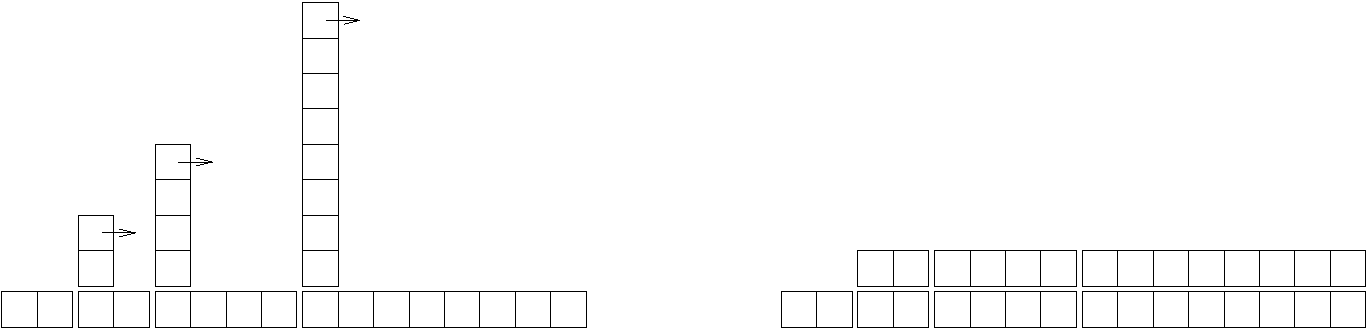
\includegraphics[width=5.5in]{../source/figs/towers.pdf}}
\caption{The cost of a hashtable add.\label{fig.hash}}
\end{figure}

The extra work of rehashing appears as a sequence of increasingly
tall towers with increasing space between them.  Now if you knock
over the towers, spreading the cost of resizing over all
adds, you can see graphically that the total cost after $n$
adds is $2n - 2$.

重哈希的额外工作显示为一序列增加的高塔并在它们之间增加空间。
现在,如果你打翻这些塔,将 resize 的代价均摊到所有的 add 上,
你会从图上看到 $n$ 个add的整个花费是 $2n - 2$ 。

An important feature of this algorithm is that when we resize the
HashTable it grows geometrically; that is, we multiply the size by a
constant.  If you increase the size
arithmetically---adding a fixed number each time---the average time
per {\tt add} is linear.

该算法一个重要的特征是当我们 resize 哈希表的时候,
它几何级增长。也就是说,我们用常数乘以大小。
如果你按算术级增加大小 —— 每次增加固定的数目—每个 \li{add} 的平均时间是线性的。
\index{geometric resizing}

You can download my implementation of HashMap from
\url{http://thinkpython2.com/code/Map.py}, but remember that there
is no reason to use it; if you want a map, just use a Python dictionary.

你可以 \href{http://thinkpython2.com/code/Map.py}{在此下载} 到 HashMap 的实现代码, 但在实际环境中直接使用 Python 的{\em 字典}足矣。

\section{Glossary  |  术语表}

\begin{description}

\item[]

\item[analysis of algorithms:] A way to compare algorithms in terms of
their run time and/or space requirements.

\item[算法分析] 比较不同算法间运行时间和资源占用的分析方法。
\index{analysis of algorithms}

\item[machine model:] A simplified representation of a computer used
to describe algorithms.

\item[模型机器] 用于描述算法(性能)的简化的计算机表示。
\index{machine model}

\item[worst case:] The input that makes a given algorithm run slowest (or
require the most space.

\item[最坏情况] 对给定算法话最长时间运行(或占用做多资源)的输入。
\index{worst case}

\item[leading term:] In a polynomial, the term with the highest exponent.

\item[首项] 在多项式中,拥有指数最高的项
\index{leading term}

\item[crossover point:] The problem size where two algorithms require
the same run time or space.

\item[交叉点] 两个算法对求解给定问题在某个规模需要相同运行时间或资源开销。
\index{crossover point}

\item[order of growth:] A set of functions that all grow in a way
considered equivalent for purposes of analysis of algorithms.
For example, all functions that grow linearly belong to the same
order of growth.

\item [增长阶数] 一些函数的组合,其函数值的增长在某种程度上等同于算法分析考察的目标。 例如, 线性递增的所有的函数都 属于 同一个增长阶数。
\index{order of growth}

\item[Big-Oh notation:] Notation for representing an order of growth;
for example, $O(n)$ represents the set of functions that grow
linearly.

\item[大O符号] 代表增长阶数的符号;例如, $O(n)$ 代表线性递增的函数。
\index{Big-Oh notation}

\item[linear:] An algorithm whose run time is proportional to
problem size, at least for large problem sizes.

\item[线性级] 算法的运行时间和所求解问题的规模成比例, 至少是在问题规模较大时显现。 
\index{linear}

\item[quadratic:] An algorithm whose run time is proportional to
$n^2$, where $n$ is a measure of problem size.

\item[二次方级] 算法的运行时间和说求解问题的规模的二次方($n^2$)成比例,$n$ 用于描述问题的规模。
\index{quadratic}

\item[search:] The problem of locating an element of a collection
(like a list or dictionary) or determining that it is not present.

\item[检索] 定位一个集合(例如列表或字典)中某个元素位置的问题,也等价于确认某元素不再该集合中的问题。
\index{search}

\item[hashtable:] A data structure that represents a collection of
key-value pairs and performs search in constant time.

\item[哈希表] 一种数据结构用于描述 键-值对 的集合,在该类集合运行检索任务只花费固定的时间(不依赖于集合的大小)。
\index{hashtable}

\end{description}


\printindex

\clearemptydoublepage

%\blankpage
%\blankpage
%\blankpage

\end{document}
